\documentclass[a4paper]{ltjsreport}
\usepackage[hiragino-pro]{luatexja-preset}
\usepackage{../hogehoge}
\newtoks\subsectiontitle
\usepackage{fancyhdr}
\pagestyle{fancy}
\lhead{}
\chead{\rightmark}
\rhead{}
\renewcommand{\subsectionmark}[1]{\markright{#1}\global\subsectiontitle{#1}}
\renewcommand{\subsubsectionmark}[1]{\markright{\the\subsectiontitle~|~#1}}
\renewcommand{\prepartname}{Part }
\renewcommand{\postpartname}{}
\renewcommand{\prechaptername}{Chapter }
\renewcommand{\postchaptername}{}
\setcounter{secnumdepth}{1}
\setcounter{tocdepth}{4}
\usepackage[backend=biber, sorting=none]{biblatex}
\addbibresource{./src/peskin_qft.bib}
\begin{document}
\chapter*{An Introduction to Quantum Field Theory (Peskin and Schroeder)}
参考本:
\begin{itemize}
  \item \cite{griffiths2020introduction} Feynmanルールの証明はせずに摂動計算の練習
  \item \cite{坂本眞人2020量子力学選書} 非可換ゲージ理論について分かりやすく書いてある
  \item \cite{romao2012resource} 標準模型のFeynman rule一覧.Higgs field \(\phi\)の定義が異なるので注意が必要
\end{itemize}

\printbibliography
\tableofcontents

\part{Feynman Diagrams and Quantum Electrodynamics}
\subsection{Fourier変換}
場のFourier変換はxxiのように
\[
\phi(x) = \int \frac{d^4k}{(2\pi)^4} e^{-ik\cdot x} \phi(k) , \quad
\phi(k) = \int d^4x \, e^{ik\cdot x} \phi(x)
\]
と定める.Fermionの場合は
\[
\psi(p) = \int d^4x \, e^{ip\cdot x} \psi(x) , \quad
\bar\psi(p) = \int d^4x \, e^{-ip\cdot x} \bar\psi(x)
\]
とする\footnote{\(\bar\psi(p)\)は\(\psi(p)\)のHermite共役に対し右から\(\gamma^0\)をかけたもの}.
Propagatorは
\begin{align*}
    \wick{\c1{\psi}(p) \c1{\bar\psi}(q)}
    &= \int d^4x \, e^{ip\cdot x} \int d^4y \, e^{-iq\cdot x} \wick{\c1{\psi}(x) \c1{\bar\psi}(y)} \\
    &= \int d^4x \, e^{ip\cdot x} \int d^4y \, e^{-iq\cdot y} \int \frac{d^4k}{(2\pi)^4} \frac{i\slashed{k}}{k^2} e^{-ik\cdot(x-y)} \\
    &= \frac{i\slashed{p}}{p^2} (2\pi)^4 \mathop{\delta^{(4)}}(p-q) .
\end{align*}

(4.47)より\(e^{-ipx}\)は位置\(x\)に運動量\(p\)が入るものとする(e.g.\@ (4.47), p.\@ 507).

\setcounter{chapter}{1}
\chapter{The Klein-Gordon Field}
\setcounter{section}{3}
\section{The Klein-Gordon Field in spacetime}
\subsection{(2.52)}
積分
\[ \int_{-\infty}^\infty dp \, \frac{p e^{ipr}}{\sqrt{p^2 + m^2}} \]
を計算する.複素平面では,$1/\sqrt{p^2+m^2}$は$p = \pm im$に極をもち,$[\pm im, \pm\infty)$を載線(branch cut)に取れる.
\begin{center}
  \begin{tikzpicture}[>=stealth]
    \draw[->] (-3, 0) -- (3, 0) node [right] {$\Re p$};
    \draw[->] (0, -1) -- (0, 3) node [above] {$\Im p$};
    \draw (0, 0) node [below left] {O};
    \fill (0, 1) circle [radius=0.1] node [right] {$im$};
    % \fill (0, -1) circle [radius=0.1] node [right] {$-im$};
    \draw[decorate, decoration={zigzag, segment length=0.2cm}, thick] (0, 1) -- (0, 2.8);
    % \draw[decorate, decoration={zigzag, segment length=0.2cm}, thick] (0, -1) -- (0, -2.8);
    \draw[->] (0, 1)+(100:0.7) arc (100:440:0.7);
  \end{tikzpicture}
\end{center}
branch cutの左右で$p^2+m^2$の偏角は$2\pi$異なるので,$\sqrt{p^2+m^2}$の偏角は$\pi$異なる.
すなわち,左右で被積分函数の符号は入れ替わる.

次の経路で,積分値は$0$.
\begin{center}
  \begin{tikzpicture}[>=stealth]
    \draw[->] (-3, 0) -- (3, 0) node [right] {$\Re p$};
    \draw[->] (0, -1) -- (0, 3) node [above] {$\Im p$};
    \draw (0, 0) node [below left] {O};
    \fill (0, 1) circle [radius=0.1];
    % \fill (0, -1) circle [radius=0.1] node [right] {$-im$};
    \draw[decorate, decoration={zigzag, segment length=0.2cm}, thick] (0, 1) -- (0, 2.8);
    % \draw[decorate, decoration={zigzag, segment length=0.2cm}, thick] (0, -1) -- (0, -2.8);
    \draw[very thick] (-0.2, 1) arc (180:360:0.2);
    \begin{scope}[very thick, decoration={markings, mark=at position 0.6 with {\arrow{stealth}}}]
      \draw[postaction={decorate}] (-0.2, 1) -- (-0.2, 2.5);
      \draw[postaction={decorate}] (-0.2, 2.5) arc (90:180:2.5);
      \draw[postaction={decorate}] (-2.7, 0) -- (2.7, 0);
      \draw[postaction={decorate}] (2.7, 0) arc (0:90:2.5);
      \draw[postaction={decorate}] (0.2, 2.5) -- (0.2, 1);
    \end{scope}
  \end{tikzpicture}
\end{center}
大きい円弧に沿った積分は$0$なので,結局,
\begin{center}
  \begin{tikzpicture}[>=stealth]
    \draw[->] (-3, 0) -- (3, 0) node [right] {$\Re p$};
    \draw[->] (0, -1) -- (0, 3) node [above] {$\Im p$};
    \draw (0, 0) node [below left] {O};
    \fill (0, 1) circle [radius=0.1];
    % \fill (0, -1) circle [radius=0.1] node [right] {$-im$};
    \draw[decorate, decoration={zigzag, segment length=0.2cm}, thick] (0, 1) -- (0, 2.8);
    % \draw[decorate, decoration={zigzag, segment length=0.2cm}, thick] (0, -1) -- (0, -2.8);
    % \draw[very thick] (-0.2, 1) arc (180:360:0.2);
    \begin{scope}[very thick, decoration={markings, mark=at position 0.6 with {\arrow{stealth}}}]
      % \draw[postaction={decorate}] (-0.2, 1) -- (-0.2, 2.5);
      % \draw[postaction={decorate}] (-0.2, 2.5) arc (90:180:2.5);
      \draw[postaction={decorate}] (-2.7, 0) -- (2.7, 0);
      % \draw[postaction={decorate}] (2.7, 0) arc (0:90:2.5);
      % \draw[postaction={decorate}] (0.2, 2.5) -- (0.2, 1);
    \end{scope}
  \end{tikzpicture}
  \raisebox{2cm}{$=$}
  \begin{tikzpicture}[>=stealth]
    \draw[->] (-3, 0) -- (3, 0) node [right] {$\Re p$};
    \draw[->] (0, -1) -- (0, 3) node [above] {$\Im p$};
    \draw (0, 0) node [below left] {O};
    \fill (0, 1) circle [radius=0.1];
    % \fill (0, -1) circle [radius=0.1] node [right] {$-im$};
    \draw[decorate, decoration={zigzag, segment length=0.2cm}, thick] (0, 1) -- (0, 2.8);
    % \draw[decorate, decoration={zigzag, segment length=0.2cm}, thick] (0, -1) -- (0, -2.8);
    \draw[very thick] (-0.2, 1) arc (180:360:0.2);
    \begin{scope}[very thick, decoration={markings, mark=at position 0.6 with {\arrow{stealth}}}]
      \draw[postaction={decorate}] (0.2, 1) -- (0.2, 2.5);
      % \draw[postaction={decorate}] (-0.2, 2.5) arc (90:180:2.5);
      % \draw[postaction={decorate}] (-2.7, 0) -- (2.7, 0);
      % \draw[postaction={decorate}] (2.7, 0) arc (0:90:2.5);
      \draw[postaction={decorate}] (-0.2, 2.5) -- (-0.2, 1);
    \end{scope}
  \end{tikzpicture}
\end{center}
左側と右側の積分は逆向きで,被積分函数の符号が逆なので,積分値は等しい.
従って,$p = i\rho$とすれば,
\[ \int_{-\infty}^\infty = 2 \int_{im}^{i\infty} dp = 2i \int_m^\infty d\rho \]
となる.

\chapter{The Dirac Field}
\section*{Problems}\addcontentsline{toc}{section}{Problems}
\subsection{Problem 3.4: The Quantized Majorana Field}
Majoranaフェルミオンのモード展開は次式で与えられる:
\begin{align*}
    \chi & = \int \frac{d^3p}{(2\pi)^3} \sqrt{\frac{(p \sigma)}{2E_{\boldsymbol{p}}}} \sum_s \left( a_{\boldsymbol{p}}^s \xi^s e^{-ipx} - i \sigma^2 a_{\boldsymbol{p}}^{s\dagger} \xi^s e^{ipx} \right) , \\
    % <!-- -->
    \chi^\dagger & = \int \frac{d^3p}{(2\pi)^3} \sqrt{\frac{1}{2E_{\boldsymbol{p}}}} \sum_s \left( a_{\boldsymbol{p}}^{s\dagger} \xi^{s\dagger} e^{ipx} + i a_{\boldsymbol{p}}^{s} \xi^{s\dagger} \sigma^2 e^{-ipx} \right) \sqrt{(p \sigma)} , \\
    % <!-- -->
    \chi^\ast & = \int \frac{d^3p}{(2\pi)^3} \sqrt{\frac{(p\sigma^\ast)}{2E_{\boldsymbol{p}}}} \sum_s \left( a_{\boldsymbol{p}}^{s\dagger} \xi^s e^{ipx} - i \sigma^2 a_{\boldsymbol{p}}^{s} \xi^s e^{-ipx} \right) , \\
    % <!-- -->
    \chi^\top & = \int \frac{d^3p}{(2\pi)^3} \sqrt{\frac{1}{2E_{\boldsymbol{p}}}} \sum_s \left( a_{\boldsymbol{p}}^{s} \xi^{s\dagger} e^{-ipx} + i a_{\boldsymbol{p}}^{s\dagger} \xi^{s\dagger} \sigma^2 e^{ipx} \right) \sqrt{(p\sigma^\top)} , \\
    % <!-- -->
    (\boldsymbol{\sigma} \cdot \boldsymbol{\nabla})\chi & = \int \frac{d^3p}{(2\pi)^3} i (\boldsymbol{p} \cdot \boldsymbol{\sigma}) \sqrt{\frac{(p \sigma)}{2E_{\boldsymbol{p}}}} \sum_s \left( a_{\boldsymbol{p}}^s \xi^s e^{-ipx} + i \sigma^2 a_{\boldsymbol{p}}^{s\dagger} \xi^s e^{ipx} \right) .
\end{align*}
ハミルトニアンは
\begin{align}
  H_\text{Majorana} = \int d^3x \left( \frac{\partial \mathcal{L}}{\partial \dot{\chi}} \dot{\chi} - \mathcal{L} \right) = \int d^3x \left[ i \chi^\dagger \boldsymbol{\sigma} \cdot \boldsymbol{\nabla} \chi + \frac{im}{2} ( \chi^\dagger \sigma^2 \chi^\ast - \chi^\top \sigma^2 \chi ) \right] . \label{prob3_4_H}
\end{align}

\eqref{prob3_4_H}第1項($e^{\pm p_0t}$は省略)は
\begin{align*}
  & \int d^3x \, i \chi^\dagger \boldsymbol{\sigma} \cdot \boldsymbol{\nabla} \chi \\
  & = \int d^3x \int \frac{d^3p\, d^3q}{(2\pi)^6} \frac{-1}{\sqrt{2E_{\boldsymbol{p}} 2 E_{\boldsymbol{q}}}}
  \sum_{r, s} \left( a_{\boldsymbol{p}}^{r\dagger} \xi^{r\dagger} e^{ipx} + i a_{\boldsymbol{p}}^{r} \xi^{r\dagger} \sigma^2 e^{-ipx} \right) \\
  & \qquad \qquad \times \sqrt{(p \sigma)} (\boldsymbol{q} \cdot \boldsymbol{\sigma}) \sqrt{(q \sigma)}
  \left( a_{\boldsymbol{q}}^s \xi^s e^{-iqx} + i \sigma^2 a_{\boldsymbol{q}}^{s\dagger} \xi^s e^{iqx} \right) \\
  % <!-- 1, 1 -->
  & = \int d^3x \int \frac{d^3p\, d^3q}{(2\pi)^6} \frac{-1}{\sqrt{2E_{\boldsymbol{p}} 2 E_{\boldsymbol{q}}}}
  \sum_{r, s} \left( a_{\boldsymbol{p}}^{r\dagger} \xi^{r\dagger} e^{ipx} \right)
  \sqrt{(p \sigma)} (\boldsymbol{q} \cdot \boldsymbol{\sigma}) \sqrt{(q \sigma)}
  \left( a_{\boldsymbol{q}}^s \xi^s e^{-iqx} \right) \\
  % <!-- 1, 2 -->
  & \qquad + \int d^3x \int \frac{d^3p\, d^3q}{(2\pi)^6} \frac{-1}{\sqrt{2E_{\boldsymbol{p}} 2 E_{\boldsymbol{q}}}}
  \sum_{r, s} \left( a_{\boldsymbol{p}}^{r\dagger} \xi^{r\dagger} e^{ipx} \right)
  \sqrt{(p \sigma)} (\boldsymbol{q} \cdot \boldsymbol{\sigma}) \sqrt{(q \sigma)}
  \left( i \sigma^2 a_{\boldsymbol{q}}^{s\dagger} \xi^s e^{iqx} \right) \\
  % <!-- 2, 1 -->
  & \qquad + \int d^3x \int \frac{d^3p\, d^3q}{(2\pi)^6} \frac{-1}{\sqrt{2E_{\boldsymbol{p}} 2 E_{\boldsymbol{q}}}}
  \sum_{r, s} \left( i a_{\boldsymbol{p}}^{r} \xi^{r\dagger} \sigma^2 e^{-ipx} \right)
  \sqrt{(p \sigma)} (\boldsymbol{q} \cdot \boldsymbol{\sigma}) \sqrt{(q \sigma)}
  \left( a_{\boldsymbol{q}}^s \xi^s e^{-iqx}\right) \\
  % <!-- 2, 2 -->
  & \qquad + \int d^3x \int \frac{d^3p\, d^3q}{(2\pi)^6} \frac{-1}{\sqrt{2E_{\boldsymbol{p}} 2 E_{\boldsymbol{q}}}}
  \sum_{r, s} \left( i a_{\boldsymbol{p}}^{r} \xi^{r\dagger} \sigma^2 e^{-ipx} \right)
  \sqrt{(p \sigma)} (\boldsymbol{q} \cdot \boldsymbol{\sigma}) \sqrt{(q \sigma)}
  \left( i \sigma^2 a_{\boldsymbol{q}}^{s\dagger} \xi^s e^{iqx} \right) \\
  % <!-- 1, 1 -->
  & = \int \frac{d^3p}{(2\pi)^3} \frac{-1}{2E_{\boldsymbol{p}}}
  \sum_{r, s} a_{\boldsymbol{p}}^{r\dagger} a_{\boldsymbol{p}}^s \times \xi^{r\dagger} \sqrt{(p \sigma)}
  (\boldsymbol{p} \cdot \boldsymbol{\sigma}) \sqrt{(p \sigma)} \xi^s \\
  % <!-- 1, 2 -->
  & \qquad + \int \frac{d^3p}{(2\pi)^3} \frac{i}{2E_{\boldsymbol{p}}}
  \sum_{r, s} a_{\boldsymbol{p}}^{r\dagger} a_{-\boldsymbol{p}}^{s\dagger}
  \times \xi^{r\dagger} \sqrt{(p \sigma)} (\boldsymbol{p} \cdot \boldsymbol{\sigma}) \sqrt{(p \bar\sigma)} \sigma^2 \xi^s \\
  % <!-- 2, 1 -->
  & \qquad + \int \frac{d^3p}{(2\pi)^3} \frac{i}{2E_{\boldsymbol{p}}}
  \sum_{r, s} a_{\boldsymbol{p}}^{r} a_{-\boldsymbol{p}}^s
  \times \xi^{r\dagger} \sigma^2 \sqrt{(p \sigma)} (\boldsymbol{p} \cdot \boldsymbol{\sigma}) \sqrt{(p \bar\sigma)} \xi^s \\
  % <!-- 2, 2 -->
  & \qquad + \int \frac{d^3p}{(2\pi)^3} \frac{1}{2E_{\boldsymbol{p}}}
  \sum_{r, s} a_{\boldsymbol{p}}^{r} a_{\boldsymbol{p}}^{s\dagger}
  \times \xi^{r\dagger} \sigma^2 \sqrt{(p \sigma)} (\boldsymbol{p} \cdot \boldsymbol{\sigma}) \sqrt{(p \sigma)} \sigma^2 \xi^s
\end{align*}
である.$\sqrt{(p\sigma)}$などを明示的に書くと
\[ \sqrt{(p \sigma)} = \frac{E_{\boldsymbol{p}} + m - \boldsymbol{p} \cdot \boldsymbol{\sigma}}{\sqrt{2 (E_{\boldsymbol{p}} + m)}} , \quad \sqrt{(p \bar\sigma)} = \frac{E_{\boldsymbol{p}} + m + \boldsymbol{p} \cdot \boldsymbol{\sigma}}{\sqrt{2 (E_{\boldsymbol{p}} + m)}} \]
となるので,
\begin{align*}
  \sqrt{(p \sigma)} (\boldsymbol{p} \cdot \boldsymbol{\sigma}) \sqrt{(p \sigma)} = E_{\boldsymbol{p}} (\boldsymbol{p} \cdot \boldsymbol{\sigma}) - \lvert \boldsymbol{p} \rvert^2 , \\
  % <!-- -->
  \sqrt{(p \sigma)} (\boldsymbol{p} \cdot \boldsymbol{\sigma}) \sqrt{(p \bar\sigma)} \sigma^2 = m (\boldsymbol{p} \cdot \boldsymbol{\sigma}) \sigma^2 , \\
  % <!-- -->
  \sigma^2 \sqrt{(p \sigma)} (\boldsymbol{p} \cdot \boldsymbol{\sigma}) \sqrt{(p \bar\sigma)} = m \sigma^2 (\boldsymbol{p} \cdot \boldsymbol{\sigma}) , \\
  % <!-- -->
  \sigma^2 \sqrt{(p \sigma)} (\boldsymbol{p} \cdot \boldsymbol{\sigma}) \sqrt{(p \sigma)} \sigma^2 = - E_{\boldsymbol{p}} (\boldsymbol{p} \cdot \boldsymbol{\sigma}^\ast) - \lvert \boldsymbol{p} \rvert^2 .
\end{align*}
従って,第1項を引き続き計算して
\begin{align}
  & = \int \frac{d^3p}{(2\pi)^3} \frac{-1}{2E_{\boldsymbol{p}}} \sum_{r, s} a_{\boldsymbol{p}}^{r\dagger} a_{\boldsymbol{p}}^s
  \times \xi^{r\dagger} \left [E_{\boldsymbol{p}} (\boldsymbol{p} \cdot \boldsymbol{\sigma}) - \lvert \boldsymbol{p} \rvert^2 \right ] \xi^s \label{prob3_4_H_1_1} \\
  % <!-- 1, 2 -->
  & + \int \frac{d^3p}{(2\pi)^3} \frac{i}{2E_{\boldsymbol{p}}} \sum_{r, s} a_{\boldsymbol{p}}^{r\dagger} a_{-\boldsymbol{p}}^{s\dagger}
  \times \xi^{r\dagger} \left[ m (\boldsymbol{p} \cdot \boldsymbol{\sigma}) \sigma^2 \right] \xi^s \label{prob3_4_H_1_2} \\
  % <!-- 2, 1 -->
  & + \int \frac{d^3p}{(2\pi)^3} \frac{i}{2E_{\boldsymbol{p}}} \sum_{r, s} a_{\boldsymbol{p}}^{r} a_{-\boldsymbol{p}}^s
  \times \xi^{r\dagger} \left [ m \sigma^2 (\boldsymbol{p} \cdot \boldsymbol{\sigma}) \right ] \xi^s \label{prob3_4_H_1_3} \\
  % <!-- 2, 2 -->
  & + \int \frac{d^3p}{(2\pi)^3} \frac{1}{2E_{\boldsymbol{p}}} \sum_{r, s} a_{\boldsymbol{p}}^{r} a_{\boldsymbol{p}}^{s\dagger}
  \times \xi^{r\dagger} \left [ - E_{\boldsymbol{p}} (\boldsymbol{p} \cdot \boldsymbol{\sigma}^\ast) - \lvert \boldsymbol{p} \rvert^2 \right ] \xi^s \label{prob3_4_H_1_4}
\end{align}
となる.

\eqref{prob3_4_H}の第2項.
\begin{align*}
  & \frac{im}{2}\int d^3x \, \chi^\dagger \sigma^2 \chi^\ast \\
  & = \frac{im}{2}\int d^3x \int \frac{d^3p\, d^3q}{(2\pi)^6} \frac{1}{\sqrt{2E_{\boldsymbol{p}}2E_{\boldsymbol{q}}}}
  \sum_{r, s} \left( a_{\boldsymbol{p}}^{r\dagger} \xi^{r\dagger} e^{ipx} + i a_{\boldsymbol{p}}^{r} \xi^{r\dagger} \sigma^2 e^{-ipx} \right) \\
  & \qquad \qquad \times \sqrt{(p \sigma)} \sigma^2 \sqrt{(q\sigma^\ast)} \left( a_{\boldsymbol{q}}^{s\dagger} \xi^s e^{iqx} - i \sigma^2 a_{\boldsymbol{q}}^{s} \xi^s e^{-iqx} \right) \\
  & = \frac{im}{2}\int d^3x \int \frac{d^3p\, d^3q}{(2\pi)^6} \frac{1}{\sqrt{2E_{\boldsymbol{p}}2E_{\boldsymbol{q}}}}
  \sum_{r, s} \left( a_{\boldsymbol{p}}^{r\dagger} \xi^{r\dagger} e^{ipx} + i a_{\boldsymbol{p}}^{r} \xi^{r\dagger} \sigma^2 e^{-ipx} \right) \\
  & \qquad \qquad \times \sqrt{(p \sigma)} \sqrt{(q\bar\sigma)} \sigma^2 \left( a_{\boldsymbol{q}}^{s\dagger} \xi^s e^{iqx} - i \sigma^2 a_{\boldsymbol{q}}^{s} \xi^s e^{-iqx} \right) \\
  % <!-- 1, 1 -->
  & = \frac{im}{2}\int d^3x \int \frac{d^3p\, d^3q}{(2\pi)^6} \frac{1}{\sqrt{2E_{\boldsymbol{p}}2E_{\boldsymbol{q}}}}
  \sum_{r, s} \left( a_{\boldsymbol{p}}^{r\dagger} \xi^{r\dagger} e^{ipx} \right) \sqrt{(p \sigma)} \sqrt{(q \bar\sigma)} \sigma^2 \left( a_{\boldsymbol{q}}^{s\dagger} \xi^s e^{iqx} \right) \\
  % <!-- 1, 2 -->
  & \qquad + \frac{im}{2}\int d^3x \int \frac{d^3p\, d^3q}{(2\pi)^6} \frac{1}{\sqrt{2E_{\boldsymbol{p}}2E_{\boldsymbol{q}}}}
  \sum_{r, s} \left( a_{\boldsymbol{p}}^{r\dagger} \xi^{r\dagger} e^{ipx} \right) \sqrt{(p \sigma)} \sqrt{(q \bar\sigma)} \sigma^2 \left( - i \sigma^2 a_{\boldsymbol{q}}^{s} \xi^s e^{-iqx} \right) \\
  % <!-- 2, 1 -->
  & \qquad + \frac{im}{2}\int d^3x \int \frac{d^3p\, d^3q}{(2\pi)^6} \frac{1}{\sqrt{2E_{\boldsymbol{p}}2E_{\boldsymbol{q}}}}
  \sum_{r, s} \left( i a_{\boldsymbol{p}}^{r} \xi^{r\dagger} \sigma^2 e^{-ipx} \right) \sqrt{(p \sigma)} \sqrt{(q \bar\sigma)} \sigma^2 \left( a_{\boldsymbol{q}}^{s\dagger} \xi^s e^{iqx} \right) \\
  % <!-- 2, 2 -->
  & \qquad + \frac{im}{2}\int d^3x \int \frac{d^3p\, d^3q}{(2\pi)^6} \frac{1}{\sqrt{2E_{\boldsymbol{p}}2E_{\boldsymbol{q}}}}
  \sum_{r, s} \left( i a_{\boldsymbol{p}}^{r} \xi^{r\dagger} \sigma^2 e^{-ipx} \right) \sqrt{(p \sigma)} \sqrt{(q \bar\sigma)} \sigma^2 \left( - i \sigma^2 a_{\boldsymbol{q}}^{s} \xi^s e^{-iqx} \right) \\
  % <!-- 1, 1 -->
  & = \frac{im}{2} \int \frac{d^3p}{(2\pi)^3} \frac{1}{2E_{\boldsymbol{p}}} \sum_{r, s} a_{\boldsymbol{p}}^{r\dagger} a_{-\boldsymbol{p}}^{s\dagger}
  \times \xi^{r\dagger} \sqrt{(p \sigma)} \sqrt{(p \sigma)} \sigma^2 \xi^s \\
  % <!-- 1, 2 -->
  & \qquad + \frac{im}{2} \int \frac{d^3p}{(2\pi)^3} \frac{-i}{2E_{\boldsymbol{p}}} \sum_{r, s} a_{\boldsymbol{p}}^{r\dagger} a_{\boldsymbol{p}}^{s}
  \times \xi^{r\dagger} \sqrt{(p \sigma)} \sqrt{(p \bar\sigma)} \xi^s \\
  % <!-- 2, 1 -->
  & \qquad + \frac{im}{2} \int \frac{d^3p}{(2\pi)^3} \frac{i}{2E_{\boldsymbol{p}}} \sum_{r, s} a_{\boldsymbol{p}}^{r} a_{\boldsymbol{p}}^{s\dagger}
  \times \xi^{r\dagger} \sigma^2 \sqrt{(p \sigma)} \sqrt{(p \bar\sigma)} \sigma^2 \xi^s \\
  % <!-- 2, 2 -->
  & \qquad + \frac{im}{2} \int \frac{d^3p}{(2\pi)^3} \frac{1}{2E_{\boldsymbol{p}}} \sum_{r, s} a_{\boldsymbol{p}}^{r} a_{-\boldsymbol{p}}^{s}
  \times \xi^{r\dagger} \sigma^2 \sqrt{(p \sigma)} \sqrt{(p \sigma)} \xi^s
\end{align*}
に$\sqrt{(p \sigma)} \sqrt{(p \bar\sigma)} = m$などを代入して,
\begin{align}
  % <!-- 1, 1 -->
  & = \frac{im}{2} \int \frac{d^3p}{(2\pi)^3} \frac{1}{2E_{\boldsymbol{p}}} \sum_{r, s} a_{\boldsymbol{p}}^{r\dagger} a_{-\boldsymbol{p}}^{s\dagger} \times \xi^{r\dagger} \left[ (p \sigma)\sigma^2 \right] \xi^s \label{prob3_4_H_2_1} \\
  % <!-- 1, 2 -->
  & + \frac{im}{2} \int \frac{d^3p}{(2\pi)^3} \frac{-im}{2E_{\boldsymbol{p}}} \sum_{r, s} a_{\boldsymbol{p}}^{r\dagger} a_{\boldsymbol{p}}^{s} \times \xi^{r\dagger} \xi^s \label{prob3_4_H_2_2} \\
  % <!-- 2, 1 -->
  & + \frac{im}{2} \int \frac{d^3p}{(2\pi)^3} \frac{im}{2E_{\boldsymbol{p}}} \sum_{r, s} a_{\boldsymbol{p}}^{r} a_{\boldsymbol{p}}^{s\dagger} \times \xi^{r\dagger} \xi^s \label{prob3_4_H_2_3} \\
  % <!-- 2, 2 -->
  & + \frac{im}{2} \int \frac{d^3p}{(2\pi)^3} \frac{1}{2E_{\boldsymbol{p}}} \sum_{r, s} a_{\boldsymbol{p}}^{r} a_{-\boldsymbol{p}}^{s} \times \xi^{r\dagger} \sigma^2 (p \sigma) \xi^s \label{prob3_4_H_2_4}
\end{align}
を得る.

\eqref{prob3_4_H}の第3項.
\begin{align*}
  & - \frac{im}{2}\int d^3x \, \chi^\top \sigma^2 \chi \\
  & = - \frac{im}{2}\int d^3x \int \frac{d^3p\,d^3q}{(2\pi)^6} \frac{1}{\sqrt{2E_{\boldsymbol{p}}2E_{\boldsymbol{q}}}}
  \sum_{r, s} \left( a_{\boldsymbol{p}}^{r} \xi^{r\dagger} e^{-ipx} + i a_{\boldsymbol{p}}^{r\dagger} \xi^{r\dagger} \sigma^2 e^{ipx} \right) \\
  & \qquad \qquad \times \sqrt{(p\sigma^\top)} \sigma^2 \sqrt{(q \sigma)} \left( a_{\boldsymbol{q}}^s \xi^s e^{-iqx} - i \sigma^2 a_{\boldsymbol{q}}^{s\dagger} \xi^s e^{iqx} \right) \\
  & = - \frac{im}{2}\int d^3x \int \frac{d^3p\,d^3q}{(2\pi)^6} \frac{1}{\sqrt{2E_{\boldsymbol{p}}2E_{\boldsymbol{q}}}}
  \sum_{r, s} \left( a_{\boldsymbol{p}}^{r} \xi^{r\dagger} e^{-ipx} + i a_{\boldsymbol{p}}^{r\dagger} \xi^{r\dagger} \sigma^2 e^{ipx} \right) \\
  & \qquad \qquad \times \sigma^2 \sqrt{(p\bar\sigma)} \sqrt{(q \sigma)} \left( a_{\boldsymbol{q}}^s \xi^s e^{-iqx} - i \sigma^2 a_{\boldsymbol{q}}^{s\dagger} \xi^s e^{iqx} \right) \\
  % <!-- 1, 1 -->
  & = - \frac{im}{2}\int d^3x \int \frac{d^3p\,d^3q}{(2\pi)^6} \frac{1}{\sqrt{2E_{\boldsymbol{p}}2E_{\boldsymbol{q}}}}
  \sum_{r, s} \left( a_{\boldsymbol{p}}^{r} \xi^{r\dagger} e^{-ipx} \right) \sigma^2 \sqrt{(p\bar\sigma)} \sqrt{(q \sigma)} \left( a_{\boldsymbol{q}}^s \xi^s e^{-iqx}\right) \\
  % <!-- 1, 2 -->
  & \qquad - \frac{im}{2}\int d^3x \int \frac{d^3p\,d^3q}{(2\pi)^6} \frac{1}{\sqrt{2E_{\boldsymbol{p}}2E_{\boldsymbol{q}}}}
  \sum_{r, s} \left( a_{\boldsymbol{p}}^{r} \xi^{r\dagger} e^{-ipx} \right) \sigma^2 \sqrt{(p\bar\sigma)} \sqrt{(q \sigma)} \left( - i \sigma^2 a_{\boldsymbol{q}}^{s\dagger} \xi^s e^{iqx} \right) \\
  % <!-- 2, 1 -->
  & \qquad - \frac{im}{2}\int d^3x \int \frac{d^3p\,d^3q}{(2\pi)^6} \frac{1}{\sqrt{2E_{\boldsymbol{p}}2E_{\boldsymbol{q}}}}
  \sum_{r, s} \left( i a_{\boldsymbol{p}}^{r\dagger} \xi^{r\dagger} \sigma^2 e^{ipx} \right) \sigma^2 \sqrt{(p\bar\sigma)} \sqrt{(q \sigma)} \left( a_{\boldsymbol{q}}^s \xi^s e^{-iqx} \right) \\
  % <!-- 2, 2 -->
  & \qquad - \frac{im}{2}\int d^3x \int \frac{d^3p\,d^3q}{(2\pi)^6} \frac{1}{\sqrt{2E_{\boldsymbol{p}}2E_{\boldsymbol{q}}}}
  \sum_{r, s} \left( i a_{\boldsymbol{p}}^{r\dagger} \xi^{r\dagger} \sigma^2 e^{ipx} \right) \sigma^2 \sqrt{(p\bar\sigma)} \sqrt{(q \sigma)} \left( - i \sigma^2 a_{\boldsymbol{q}}^{s\dagger} \xi^s e^{iqx} \right) \\
  % <!-- 1, 1 -->
  & = - \frac{im}{2}\int \frac{d^3p}{(2\pi)^3} \frac{1}{2E_{\boldsymbol{p}}} \sum_{r, s} a_{\boldsymbol{p}}^{r} a_{-\boldsymbol{p}}^s
  \times \xi^{r\dagger} \sigma^2 \sqrt{(p\bar\sigma)} \sqrt{(p \bar\sigma)} \xi^s \\
  % <!-- 1, 2 -->
  & \qquad - \frac{im}{2}\int \frac{d^3p}{(2\pi)^3} \frac{-i}{2E_{\boldsymbol{p}}} \sum_{r, s} a_{\boldsymbol{p}}^{r} a_{\boldsymbol{p}}^{s\dagger}
  \times \xi^{r\dagger} \sigma^2 \sqrt{(p\bar\sigma)} \sqrt{(p \sigma)} \sigma^2 \xi^s \\
  % <!-- 2, 1 -->
  & \qquad - \frac{im}{2}\int \frac{d^3p}{(2\pi)^3} \frac{i}{2E_{\boldsymbol{p}}} \sum_{r, s} a_{\boldsymbol{p}}^{r\dagger} a_{\boldsymbol{p}}^s
  \times \xi^{r\dagger} \sigma^2 \sigma^2 \sqrt{(p\bar\sigma)} \sqrt{(p \sigma)} \xi^s \\
  % <!-- 2, 2 -->
  & \qquad - \frac{im}{2}\int \frac{d^3p}{(2\pi)^3} \frac{1}{2E_{\boldsymbol{p}}} \sum_{r, s} a_{\boldsymbol{p}}^{r\dagger} a_{-\boldsymbol{p}}^{s\dagger}
  \times \xi^{r\dagger} \sigma^2 \sigma^2 \sqrt{(p\bar\sigma)} \sqrt{(p \bar\sigma)} \sigma^2 \xi^s
\end{align*}
となるので,
\begin{align}
  % <!-- 1, 1 -->
  & = - \frac{im}{2}\int \frac{d^3p}{(2\pi)^3} \frac{1}{2E_{\boldsymbol{p}}} \sum_{r, s} a_{\boldsymbol{p}}^{r} a_{-\boldsymbol{p}}^s
  \times \xi^{r\dagger} \left[ \sigma^2 (p\bar\sigma) \right] \xi^s \label{prob3_4_H_3_1} \\
  % <!-- 1, 2 -->
  & \quad - \frac{im}{2}\int \frac{d^3p}{(2\pi)^3} \frac{-im}{2E_{\boldsymbol{p}}} \sum_{r, s} a_{\boldsymbol{p}}^{r} a_{\boldsymbol{p}}^{s\dagger} \times \xi^{r\dagger} \xi^s \label{prob3_4_H_3_2} \\
  % <!-- 2, 1 -->
  & \quad - \frac{im}{2}\int \frac{d^3p}{(2\pi)^3} \frac{im}{2E_{\boldsymbol{p}}} \sum_{r, s} a_{\boldsymbol{p}}^{r\dagger} a_{\boldsymbol{p}}^s \times \xi^{r\dagger} \xi^s \label{prob3_4_H_3_3} \\
  % <!-- 2, 2 -->
  & \quad - \frac{im}{2}\int \frac{d^3p}{(2\pi)^3} \frac{1}{2E_{\boldsymbol{p}}} \sum_{r, s} a_{\boldsymbol{p}}^{r\dagger} a_{-\boldsymbol{p}}^{s\dagger}
  \times \xi^{r\dagger} \left[ (p\bar\sigma) \sigma^2 \right] \xi^s \label{prob3_4_H_3_4}
\end{align}
を得る.

% <!-- a+, a -->
$a_{\boldsymbol{p}}^{r\dagger} a_{\boldsymbol{p}}^{s}$の項は次のようになる:
\begin{align}
  & \eqref{prob3_4_H_1_1} + \eqref{prob3_4_H_2_2} + \eqref{prob3_4_H_3_3} \notag \\
  & = \int \frac{d^3p}{(2\pi)^3} \frac{-1}{2E_{\boldsymbol{p}}} \sum_{r, s} a_{\boldsymbol{p}}^{r\dagger} a_{\boldsymbol{p}}^s
  \times \xi^{r\dagger} \left [E_{\boldsymbol{p}} (\boldsymbol{p} \cdot \boldsymbol{\sigma}) - \lvert \boldsymbol{p} \rvert^2 \right ] \xi^s \notag \\
  & \qquad + \frac{im}{2} \int \frac{d^3p}{(2\pi)^3} \frac{-im}{2E_{\boldsymbol{p}}}
  \sum_{r, s} a_{\boldsymbol{p}}^{r\dagger} a_{\boldsymbol{p}}^{s} \times \xi^{r\dagger} \xi^s \notag \\
  & \qquad - \frac{im}{2}\int \frac{d^3p}{(2\pi)^3} \frac{im}{2E_{\boldsymbol{p}}} \sum_{r, s} a_{\boldsymbol{p}}^{r\dagger} a_{\boldsymbol{p}}^s \times \xi^{r\dagger} \xi^s \notag \\
  & = \int \frac{d^3p}{(2\pi)^3} \frac{1}{2E_{\boldsymbol{p}}} \sum_{r, s} a_{\boldsymbol{p}}^{r\dagger} a_{\boldsymbol{p}}^s
  \times \xi^{r\dagger} \left [ - E_{\boldsymbol{p}} (\boldsymbol{p} \cdot \boldsymbol{\sigma}) + \lvert \boldsymbol{p} \rvert^2 \right ] \xi^s + \int \frac{d^3p}{(2\pi)^3} \frac{m^2}{2E_{\boldsymbol{p}}}
  \sum_{r, s} a_{\boldsymbol{p}}^{r\dagger} a_{\boldsymbol{p}}^{s} \times \xi^{r\dagger} \xi^s \notag \\
  & = \int \frac{d^3p}{(2\pi)^3} \frac{\lvert \boldsymbol{p} \rvert^2 + m^2}{2E_{\boldsymbol{p}}}
  \sum_{r, s} a_{\boldsymbol{p}}^{r\dagger} a_{\boldsymbol{p}}^s \times \xi^{r\dagger} \xi^s - \int \frac{d^3p}{(2\pi)^3} \frac{1}{2}
  \sum_{r, s} a_{\boldsymbol{p}}^{r\dagger} a_{\boldsymbol{p}}^{s} \times \xi^{r\dagger} (\boldsymbol{p} \cdot \boldsymbol{\sigma}) \xi^s \notag \\
  & = \int \frac{d^3p}{(2\pi)^3} \frac{E_{\boldsymbol{p}}}{2} \sum_{r, s} a_{\boldsymbol{p}}^{r\dagger} a_{\boldsymbol{p}}^s \delta^{rs} - \int \frac{d^3p}{(2\pi)^3} \frac{1}{2}
  \sum_{r, s} a_{\boldsymbol{p}}^{r\dagger} a_{\boldsymbol{p}}^{s} \times \xi^{r\dagger} (\boldsymbol{p} \cdot \boldsymbol{\sigma}) \xi^s \notag \\
  & = \int \frac{d^3p}{(2\pi)^3} \frac{E_{\boldsymbol{p}}}{2} \sum_{s} a_{\boldsymbol{p}}^{s\dagger} a_{\boldsymbol{p}}^s \label{prob3_4_ca}
\end{align}
(最後の式変形では被積分函数が奇函数であることを使った).
$a_{\boldsymbol{p}}^{r} a_{\boldsymbol{p}}^{s\dagger}$の項は次のようになる:
\begin{align}
  & \eqref{prob3_4_H_1_4} + \eqref{prob3_4_H_2_3} + \eqref{prob3_4_H_3_2} \notag \\
  & = \int \frac{d^3p}{(2\pi)^3} \frac{1}{2E_{\boldsymbol{p}}} \sum_{r, s} a_{\boldsymbol{p}}^{r} a_{\boldsymbol{p}}^{s\dagger}
  \times \xi^{r\dagger} \left [ - E_{\boldsymbol{p}} (\boldsymbol{p} \cdot \boldsymbol{\sigma}^\ast) - \lvert \boldsymbol{p} \rvert^2 \right ] \xi^s \notag \\
  & \qquad + \frac{im}{2} \int \frac{d^3p}{(2\pi)^3} \frac{im}{2E_{\boldsymbol{p}}} \sum_{r, s} a_{\boldsymbol{p}}^{r} a_{\boldsymbol{p}}^{s\dagger} \times \xi^{r\dagger} \xi^s \notag \\
  & - \frac{im}{2}\int \frac{d^3p}{(2\pi)^3} \frac{-im}{2E_{\boldsymbol{p}}} \sum_{r, s} a_{\boldsymbol{p}}^{r} a_{\boldsymbol{p}}^{s\dagger} \times \xi^{r\dagger} \xi^s \notag \\
  & = \int \frac{d^3p}{(2\pi)^3} \frac{1}{2E_{\boldsymbol{p}}} \sum_{r, s} a_{\boldsymbol{p}}^{r} a_{\boldsymbol{p}}^{s\dagger}
  \times \xi^{r\dagger} \left [ - E_{\boldsymbol{p}} (\boldsymbol{p} \cdot \boldsymbol{\sigma}^\ast) - \lvert \boldsymbol{p} \rvert^2 \right ] \xi^s - \int \frac{d^3p}{(2\pi)^3} \frac{m^2}{2E_{\boldsymbol{p}}}
  \sum_{r, s} a_{\boldsymbol{p}}^{r} a_{\boldsymbol{p}}^{s\dagger} \times \xi^{r\dagger} \xi^s \notag \\
  & = - \int \frac{d^3p}{(2\pi)^3} \frac{\lvert \boldsymbol{p} \rvert^2 + m^2}{2E_{\boldsymbol{p}}}
  \sum_{r, s} a_{\boldsymbol{p}}^{r} a_{\boldsymbol{p}}^{s\dagger} \times \xi^{r\dagger} \xi^s - \int \frac{d^3p}{(2\pi)^3} \frac{1}{2}
  \sum_{r, s} a_{\boldsymbol{p}}^{r} a_{\boldsymbol{p}}^{s\dagger} \times \xi^{r\dagger} (\boldsymbol{p} \cdot \boldsymbol{\sigma}^\ast) \xi^s \notag \\
  & = - \int \frac{d^3p}{(2\pi)^3} \frac{E_{\boldsymbol{p}}}{2}
  \sum_{r, s} a_{\boldsymbol{p}}^{r} a_{\boldsymbol{p}}^{s\dagger} \delta^{rs} - \int \frac{d^3p}{(2\pi)^3} \frac{1}{2}
  \sum_{r, s} a_{\boldsymbol{p}}^{r} a_{\boldsymbol{p}}^{s\dagger} \times \xi^{r\dagger} (\boldsymbol{p} \cdot \boldsymbol{\sigma}^\ast) \xi^s \notag \\
  & = - \int \frac{d^3p}{(2\pi)^3} \frac{E_{\boldsymbol{p}}}{2} \sum_{s} a_{\boldsymbol{p}}^{s} a_{\boldsymbol{p}}^{s\dagger} \label{prob3_4_ac}
\end{align}
(最後の式変形では被積分函数が奇函数であることを使った).
$a_{\boldsymbol{p}}^{r\dagger} a_{-\boldsymbol{p}}^{s\dagger}$の項は次のようになる:
\begin{align}
  & \eqref{prob3_4_H_1_2} + \eqref{prob3_4_H_2_1} + \eqref{prob3_4_H_3_4} \notag \\
  & = \int \frac{d^3p}{(2\pi)^3} \frac{i}{2E_{\boldsymbol{p}}}
  \sum_{r, s} a_{\boldsymbol{p}}^{r\dagger} a_{-\boldsymbol{p}}^{s\dagger} \times \xi^{r\dagger} \left[ m (\boldsymbol{p} \cdot \boldsymbol{\sigma}) \sigma^2 \right] \xi^s \notag \\
  & \qquad + \frac{im}{2} \int \frac{d^3p}{(2\pi)^3} \frac{1}{2E_{\boldsymbol{p}}} \sum_{r, s} a_{\boldsymbol{p}}^{r\dagger} a_{-\boldsymbol{p}}^{s\dagger} \times \xi^{r\dagger} \left[ (p \sigma)\sigma^2 \right] \xi^s \notag \\
  & \qquad - \frac{im}{2}\int \frac{d^3p}{(2\pi)^3} \frac{1}{2E_{\boldsymbol{p}}} \sum_{r, s} a_{\boldsymbol{p}}^{r\dagger} a_{-\boldsymbol{p}}^{s\dagger} \times \xi^{r\dagger} \left[ (p\bar\sigma) \sigma^2 \right] \xi^s \notag \\
  & = 0 . \label{prob3_4_cc}
\end{align}
$a_{\boldsymbol{p}}^{r} a_{-\boldsymbol{p}}^{s}$の項は次のようになる:
\begin{align}
  & \eqref{prob3_4_H_1_3} + \eqref{prob3_4_H_2_4} + \eqref{prob3_4_H_3_1} \notag \\
  & = \int \frac{d^3p}{(2\pi)^3} \frac{i}{2E_{\boldsymbol{p}}} \sum_{r, s} a_{\boldsymbol{p}}^{r} a_{-\boldsymbol{p}}^s \times \xi^{r\dagger} \left [ m \sigma^2 (\boldsymbol{p} \cdot \boldsymbol{\sigma}) \right ] \xi^s \notag \\
  & \qquad + \frac{im}{2} \int \frac{d^3p}{(2\pi)^3} \frac{1}{2E_{\boldsymbol{p}}} \sum_{r, s} a_{\boldsymbol{p}}^{r} a_{-\boldsymbol{p}}^{s} \times \xi^{r\dagger} \sigma^2 (p \sigma) \xi^s \notag \\
  & \qquad - \frac{im}{2}\int \frac{d^3p}{(2\pi)^3} \frac{1}{2E_{\boldsymbol{p}}} \sum_{r, s} a_{\boldsymbol{p}}^{r} a_{-\boldsymbol{p}}^s \times \xi^{r\dagger} \left[ \sigma^2 (p\bar\sigma) \right] \xi^s \notag \\
  & = 0 . \label{prob3_4_aa}
\end{align}
\eqref{prob3_4_ca}\eqref{prob3_4_ac}\eqref{prob3_4_cc}\eqref{prob3_4_aa}から,
\begin{align*}
  H_\text{Majorana} & = \int \frac{d^3p}{(2\pi)^3} \frac{E_{\boldsymbol{p}}}{2} \sum_{s} a_{\boldsymbol{p}}^{s\dagger} a_{\boldsymbol{p}}^s - \int \frac{d^3p}{(2\pi)^3} \frac{E_{\boldsymbol{p}}}{2} \sum_{s} a_{\boldsymbol{p}}^{s} a_{\boldsymbol{p}}^{s\dagger} \\
  & = \int \frac{d^3p}{(2\pi)^3} E_{\boldsymbol{p}} \sum_{s} a_{\boldsymbol{p}}^{s\dagger} a_{\boldsymbol{p}}^s
\end{align*}
となる(最後の計算では,発散する定数を無視した).これはDirac場のハミルトニアン
\[ H_\text{Dirac} = \int \frac{d^3p}{(2\pi)^3} E_{\boldsymbol{p}} \sum_{s} \left( a_{\boldsymbol{p}}^{s\dagger} a_{\boldsymbol{p}}^s + b_{\boldsymbol{p}}^{s\dagger} b_{\boldsymbol{p}}^s \right) \]
の半分である.

\chapter{Interacting Fields and Feynman Diagrams}
\section*{Problems}\addcontentsline{toc}{section}{Problems}
\subsection{Problem 4.2: Linear sigma model}
\subsubsection{(d)}
ポテンシャルは
\[ V = -\frac{1}{2} \mu^2 \boldsymbol\Phi \cdot \boldsymbol\Phi + \frac{\lambda}{4} (\boldsymbol\Phi \cdot \boldsymbol\Phi)^2 - a \Phi^N  \]
で与えられる.$V$が$\Phi^i = 0$で極小となる$v$を求める.
\[ \frac{\partial V}{\partial \Phi^i} = (-\mu^2 + \lambda \boldsymbol\Phi \cdot \boldsymbol\Phi) \Phi^i - a \delta^{iN} \]
に$\Phi^i = 0 ~ (1 \leq i \leq N-1)$, $\Phi^N = v$を代入して,
\[ (-\mu^2 + \lambda v^2) v \delta^{iN} - a \delta^{iN} = 0 .\]
$a$は十分小さいので,
\[ v = \frac{\mu}{\sqrt{\lambda}} + \frac{a}{2\mu^2} \]
であり,
\[ \Phi^N = \frac{\mu}{\sqrt{\lambda}} + \sigma + \frac{a}{2\mu^2} . \]

$V$の表式は
\begin{align*}
  V &= -\frac{1}{2} \mu^2 \boldsymbol\Phi \cdot \boldsymbol\Phi + \frac{\lambda}{4} (\boldsymbol\Phi \cdot \boldsymbol\Phi)^2 - a \Phi^N \\
  &= -\frac{\mu^2}{2} \left\{ \boldsymbol\pi \cdot \boldsymbol\pi + \left( \frac{\mu}{\sqrt{\lambda}} + \sigma + \frac{a}{2\mu^2} \right)^2 \right\}
  + \frac{\lambda}{4} \left\{ \boldsymbol\pi \cdot \boldsymbol\pi + \left( \frac{\mu}{\sqrt{\lambda}} + \sigma + \frac{a}{2\mu^2} \right)^2 \right\}^2
  - a \left( \frac{\mu}{\sqrt{\lambda}} + \sigma + \frac{a}{2\mu^2} \right) \\
  &\simeq -\frac{\mu^2}{2} \left\{ \boldsymbol\pi \cdot \boldsymbol\pi + \left( \frac{\mu}{\sqrt{\lambda}} + \sigma\right)^2 + 2 \left( \frac{\mu}{\sqrt{\lambda}} + \sigma\right)\frac{a}{2\mu^2} \right\} \\
  & \quad + \frac{\lambda}{4} \left[ \left\{ \boldsymbol\pi \cdot \boldsymbol\pi + \left( \frac{\mu}{\sqrt{\lambda}} + \sigma\right)^2 \right\}^2
  + 2 \left\{ \boldsymbol\pi \cdot \boldsymbol\pi + \left( \frac{\mu}{\sqrt{\lambda}} + \sigma\right)^2 \right\} 2 \left( \frac{\mu}{\sqrt{\lambda}} + \sigma\right)\frac{a}{2\mu^2} \right] \\
  & \quad - a \left( \frac{\mu}{\sqrt{\lambda}} + \sigma \right).
\end{align*}
$a$を含まない項を先に計算する(これは(b)で計算した):
\begin{align*}
  V_0 &= -\frac{\mu^2}{2} \left\{ \boldsymbol\pi \cdot \boldsymbol\pi + \left( \frac{\mu}{\sqrt{\lambda}} + \sigma\right)^2 \right\}
  + \frac{\lambda}{4} \left\{ \boldsymbol\pi \cdot \boldsymbol\pi + \left( \frac{\mu}{\sqrt{\lambda}} + \sigma\right)^2 \right\}^2 \\
  &= -\frac{\mu^2}{2} (\boldsymbol\pi \cdot \boldsymbol\pi) - \frac{\mu^2}{2} \left( \frac{\mu^2}{\lambda} + 2\frac{\mu}{\sqrt{\lambda}}\sigma + \sigma^2 \right)
  + \frac{\lambda}{4} \left\{ (\boldsymbol\pi \cdot \boldsymbol\pi) + \left( \frac{\mu^2}{\lambda} + 2\frac{\mu}{\sqrt{\lambda}}\sigma + \sigma^2 \right) \right\}^2 \\
  &= -\frac{\mu^2}{2} (\boldsymbol\pi \cdot \boldsymbol\pi) - \frac{\mu^2}{2} \left( \frac{\mu^2}{\lambda} + 2\frac{\mu}{\sqrt{\lambda}}\sigma + \sigma^2 \right) \\
  &\quad + \frac{\lambda}{4} \left\{ (\boldsymbol\pi \cdot \boldsymbol\pi) + 2 (\boldsymbol\pi \cdot \boldsymbol\pi) \left( \frac{\mu^2}{\lambda}
  + 2\frac{\mu}{\sqrt{\lambda}}\sigma + \sigma^2 \right) + \left( \frac{\mu^2}{\lambda} + 2\frac{\mu}{\sqrt{\lambda}}\sigma + \sigma^2 \right)^2 \right\} \\
  &= -\frac{\mu^2}{2} (\boldsymbol\pi \cdot \boldsymbol\pi) - \frac{\mu^4}{2\lambda} - \frac{\mu^3}{\sqrt{\lambda}}\sigma - \frac{\mu^2}{2}\sigma^2 \\
  &\quad + \frac{\lambda}{4}(\boldsymbol\pi \cdot \boldsymbol\pi)^2 + \frac{\mu^2}{2}(\boldsymbol\pi \cdot \boldsymbol\pi) + \sqrt{\lambda}\mu (\boldsymbol\pi \cdot \boldsymbol\pi) \sigma + \frac{\lambda}{2} (\boldsymbol\pi \cdot \boldsymbol\pi) \sigma^2 \\
  &\quad + \frac{\mu^4}{4\lambda} + \mu^2\sigma^2 + \frac{\lambda}{4}\sigma^4 + \frac{\mu^3}{\sqrt{\lambda}}\sigma + \frac{1}{2}\mu^2\sigma^2 + \sqrt{\lambda}\mu\sigma^3 \\
  &= - \frac{\mu^4}{4\lambda} + \sqrt{\lambda}\mu\sigma^3 + \mu^2\sigma^2 + \frac{\lambda}{4}\sigma^4 + \frac{\lambda}{4}(\boldsymbol\pi \cdot \boldsymbol\pi)^2
  + \sqrt{\lambda}\mu (\boldsymbol\pi \cdot \boldsymbol\pi) \sigma + \frac{\lambda}{2} (\boldsymbol\pi \cdot \boldsymbol\pi) \sigma^2 .
\end{align*}
次に,$a$を含む項を計算する:
\begin{align*}
  V_a &= -\mu^2 \left( \frac{\mu}{\sqrt{\lambda}} + \sigma\right)\frac{a}{2\mu^2}
  + \lambda \left\{ \boldsymbol\pi \cdot \boldsymbol\pi + \left( \frac{\mu}{\sqrt{\lambda}} + \sigma\right)^2 \right\} \left( \frac{\mu}{\sqrt{\lambda}} + \sigma\right)\frac{a}{2\mu^2}
  - a \left( \frac{\mu}{\sqrt{\lambda}} + \sigma \right) \\
  &= a \left( \frac{\mu}{\sqrt{\lambda}} + \sigma \right) \left\{ -\frac{3}{2} + \frac{\lambda}{2\mu^2} \left( \boldsymbol\pi \cdot \boldsymbol\pi + \frac{\mu^2}{\lambda} + 2\frac{\mu}{\sqrt{\lambda}}\sigma + \sigma^2 \right) \right\} \\
  &= a \left( \frac{\mu}{\sqrt{\lambda}} + \sigma \right) \frac{\lambda}{2\mu^2} \left( \boldsymbol\pi \cdot \boldsymbol\pi - 2\frac{\mu^2}{\lambda} + 2\frac{\mu}{\sqrt{\lambda}}\sigma + \sigma^2 \right).
\end{align*}
以上から
\begin{align*}
  V &= V_0 + V_a \\
  &= \frac{1}{2}\left( 2\mu^2 + \frac{3a\sqrt{\lambda}}{\mu} \right) \sigma^2 + \frac{1}{2} \frac{a\sqrt{\lambda}}{\mu} (\boldsymbol\pi \cdot \boldsymbol\pi) \\
  &\quad + \left( \sqrt{\lambda}\mu + \frac{a\lambda}{2\mu^2} \right) (\boldsymbol\pi \cdot \boldsymbol\pi) \sigma + \left( \sqrt{\lambda}\mu
  + \frac{a\lambda}{2\mu^2} \right) \sigma^3 + \frac{\lambda}{4} (\boldsymbol\pi \cdot \boldsymbol\pi)^2 + \frac{\lambda}{2} (\boldsymbol\pi \cdot \boldsymbol\pi) \sigma^2 + \frac{\lambda}{4} \sigma^4 \\
  &\quad + \text{const}.
\end{align*}

質量は
\[ m_\sigma{}^2 = 2\mu^2 + \frac{3a\sqrt{\lambda}}{\mu} , \quad m_\pi{}^2 = \frac{a\sqrt{\lambda}}{\mu} . \]
propagatorは
\begin{align*}
  \feynmandiagram[horizontal=a to b]{a -- [doublefermion] b};
  &= \int \frac{d^4p}{(2\pi)^4} \frac{i}{p^2 - m_\sigma{}^2 + i\epsilon} e^{-ip(x-y)} , \\
  \feynmandiagram[horizontal=a to b]{a -- [fermion] b};
  &= \int \frac{d^4p}{(2\pi)^4} \frac{i}{p^2 - m_\pi{}^2 + i\epsilon} e^{-ip(x-y)} \delta^{ij}.
\end{align*}
vertex factorは
\begin{align*}
  \feynmandiagram[vertical=a to b, inline=(b.base)]{i1 [particle=$j$] -- b -- i2 [particle=$i$] , a -- [double] b};
  &= -2i \left( \sqrt{\lambda}\mu + \frac{a\lambda}{2\mu^2} \right) \delta^{ij} \\
  %
  \feynmandiagram[vertical=a to b, inline=(b.base)]{i1 -- [double] b -- [double] i2 , a -- [double] b};
  &= -6i \left( \sqrt{\lambda}\mu + \frac{a\lambda}{2\mu^2} \right) \\
  %
  \feynmandiagram[horizontal=i1 to f1, inline=(c.base)]{i1 [particle=$k$] -- c [dot] -- i2 [particle=$j$], f1 [particle=$l$] -- c -- f2 [particle=$i$]};
  &= -2i\lambda \left( \delta^{ij}\delta^{kl} + \delta^{il}\delta^{jk} + \delta^{ik}\delta^{jl} \right) \\
  %
  \feynmandiagram[horizontal=i1 to f1, inline=(c.base)]{i1 -- [double] c [dot] -- i2 [particle=$j$], f1 -- [double] c -- f2 [particle=$i$]};
  &= -2i\lambda \delta^{ij} \\
  %
  \feynmandiagram[horizontal=i1 to f1, inline=(c.base)]{i1 -- [double] c [dot] -- [double] i2, f1 -- [double] c -- [double] f2};
  &= -6i\lambda
\end{align*}
で与えられる.

$T$行列要素
\[ T = \Braket{ p_3^k p_4^l | T \exp\left( - \int d^4x\, \mathcal{H}_\text{int} \right) | p_1^i p_2^j } \]
を計算する.

まず,$2$次の展開を考える:
\[ \sum_{m, n} \Braket{ 0 | a_{\boldsymbol{p_3}}^k a_{\boldsymbol{p_4}}^l \frac{(-i)^2}{2!} (\sqrt{\lambda}\mu)^2 \int d^4x d^4y\,
N\{ \pi^m(y) \pi^m(y) \sigma(y) \pi^n(x) \pi^n(x) \sigma(x) \} a_{\boldsymbol{p_1}}^{i\dagger} a_{\boldsymbol{p_2}}^{j\dagger} | 0 } . \]

\begin{center}
  \feynmandiagram [vertical=b to a] {
  i1 [particle=$j$] -- [momentum'=$p_2$] a, i2 [particle=$i$] -- [momentum=$p_1$] a,
  a [label=270:$x$] -- [double,  momentum'=$q$] b [label=90:$y$],
  b -- [momentum=$p_3$] f1 [particle=$k$], b -- [momentum'=$p_4$] f2 [particle=$l$]
  };
\end{center}
上図に対応する項は$4$通り存在し,$x$と$y$の交換を考慮に入れて,
\begin{align*}
  &\quad -4\lambda\mu^2 \int d^4x d^4y \, e^{i(p_3+p_4)y} \int \frac{d^4q}{(2\pi^4)} \frac{ie^{iq(y-x)}}{q^2 - m_\sigma{}^2} e^{-i(p_1+p_2)x} \delta^{ij}\delta^{kl} \\
  &= -4\lambda\mu^2 \int \frac{d^4q}{(2\pi^4)} \frac{1}{q^2 - m_\sigma{}^2} \int d^4y \, e^{i(p_3+p_4-q)y} \int d^4x \, e^{-i(p_1+p_2-q)x} \delta^{ij}\delta^{kl} \\
  &= -(2\pi)^4 4i\lambda\mu^2 \int \frac{d^4q}{q^2 - m_\sigma{}^2} \mathop{\delta^{(4)}}(p_3+p_4-q) \mathop{\delta^{(4)}}(p_1+p_2-q) \delta^{ij}\delta^{kl} \\
  &= \frac{-4\lambda\mu^2}{(p_1+p_2)^2 - m_\sigma{}^2} \delta^{ij}\delta^{kl} i(2\pi)^4 \mathop{\delta^{(4)}}(p_1+p_2-p_3-p_4).
\end{align*}

\begin{center}
  \feynmandiagram [horizontal=a to b] {
  i1 [particle=$i$] -- [momentum'=$p_1$] a -- [momentum'=$p_3$] i2 [particle=$k$],
  a -- [double,  momentum'=$q$] b,
  f2 [particle=$l$] -- [reversed momentum'=$p_4$] b -- [reversed momentum'=$p_2$] f1 [particle=$j$]
  };
\end{center}
この場合は
\[ \frac{-4\lambda\mu^2}{(p_1-p_3)^2 - m_\sigma{}^2} \delta^{ik}\delta^{jl} i(2\pi)^4 \mathop{\delta^{(4)}}(p_1+p_2-p_3-p_4). \]

\begin{center}
  \begin{tikzpicture}[arrowlabel/.style={/tikzfeynman/momentum/.cd, arrow shorten=0.37, arrow distance=1.5mm}, arrowlabel/.default=0.4]
    \begin{feynman}
      \vertex (a);
      \vertex [right=of a] (b);
      \vertex [below left=of a] (i1) {$i$};
      \vertex [above left=of a] (f1) {$k$};
      \vertex [below right=of b] (i2) {$j$};
      \vertex [above right=of b] (f2) {$l$};
      \diagram* {
      (i1) -- [momentum'=$p_1$] (a), (i2) -- [momentum=$p_2$] (b),
      (a) -- [double, momentum'=$q$] (b),
      (a) -- [momentum={[arrowlabel]}, edge label=$p_4$, near end] (f2), (b) -- [momentum'={[arrowlabel]}, edge label'=$p_3$, near end] (f1)
      };
    \end{feynman}
  \end{tikzpicture}
\end{center}
この場合は
\[ \frac{-4\lambda\mu^2}{(p_1-p_4)^2 - m_\sigma{}^2} \delta^{il}\delta^{jk} i(2\pi)^4 \mathop{\delta^{(4)}}(p_1+p_2-p_3-p_4). \]

\begin{center}
  \feynmandiagram[horizontal=i1 to f1, inline=(c.base)]{i1 [particle=$k$] -- [rmomentum'=$p_3$] c [dot] -- [rmomentum=$p_2$] i2 [particle=$j$],
  f1 [particle=$l$] -- [rmomentum'=$p_4$] c -- [rmomentum=$p_1$] f2 [particle=$i$]};
\end{center}
この場合は
\[ -2i\lambda \left( \delta^{ij}\delta^{kl} + \delta^{il}\delta^{jk} + \delta^{ik}\delta^{jl} \right) i(2\pi)^4 \mathop{\delta^{(4)}}(p_1+p_2-p_3-p_4). \]

$\Delta V$によって$m_\sigma{}^2 \neq 2\mu^2$となったので,$p_i \to 0$の極限でも,これらの和は$0$とならない.

\chapter{Elementary Processes of Quantum Electrodynamics}
\setcounter{section}{1}
\section{$e^+e^- \to \mu^+\mu^-$: Helicity Structure}
\subsection{(5.28)}
Dirac方程式の解は(A.19)で与えられる:
\[
u^s(p) =
\begin{pmatrix}
  \sqrt{p \cdot \sigma} \xi^s \\[5pt]
  \sqrt{p \cdot \overline\sigma} \xi^s
\end{pmatrix}
, \quad
v^s(p) =
\begin{pmatrix}
  \sqrt{p \cdot \sigma} \eta^s \\[5pt]
  - \sqrt{p \cdot \overline\sigma} \eta^s
\end{pmatrix}
.
\]
高エネルギー極限では(A.20)のように,
\[
u^s(p) \approx \sqrt{2E}
\begin{pmatrix}
  \frac{1}{2} (1 - \hat{p} \cdot \boldsymbol\sigma) \xi^s \\[5pt]
  \frac{1}{2} (1 + \hat{p} \cdot \boldsymbol\sigma) \xi^s
\end{pmatrix}
, \quad
v^s(p) \approx \sqrt{2E}
\begin{pmatrix}
  \frac{1}{2} (1 - \hat{p} \cdot \boldsymbol\sigma) \eta^s \\[5pt]
  - \frac{1}{2} (1 + \hat{p} \cdot \boldsymbol\sigma) \eta^s
\end{pmatrix}
.
\]

\begin{screen}
  電子のspinorは\(\xi={}^\top(1, 0)\)が\(+z\) (\(\sigma^3\xi=+\xi\)).
  陽電子のspinorは\(\eta={}^\top(0, 1)\)が\(+z\)(電子と逆)(p.\@ 61)
\end{screen}
\begin{screen}
  2成分のspinor $\xi$が$(\hat{p} \cdot \boldsymbol\sigma) \xi = + \xi$を満たすときhelicityを右と定義する.
  陽電子の場合はspinorと粒子のspinが逆なので,helicityも逆になる(p.\@ 142, 144)
\end{screen}

電子は$z$方向のspin上向きなので,spinorは$\xi = {}^\top(1, 0)$.
$\hat{p} = (0, 0, 1)$の向きに進むので,helicityは右.
$\hat{p}\cdot\boldsymbol\sigma = \sigma^3$なので,
\[
u \approx \sqrt{2E}
\begin{pmatrix}
  \frac{1}{2} (1 - \hat{p} \cdot \boldsymbol\sigma) \xi \\[5pt]
  \frac{1}{2} (1 + \hat{p} \cdot \boldsymbol\sigma) \xi
\end{pmatrix}
\\
= \sqrt{2E}
\begin{pmatrix}
  0 \\
  0 \\
  1 \\
  0
\end{pmatrix}
.
\]

陽電子は$z$方向の粒子spinが上向きなので,spinorは$\eta = {}^\top(0, 1)$.
$\hat{p} = (0, 0, -1)$の向きに進むので,粒子helicityは左.
$\hat{p}\cdot\boldsymbol\sigma = - \sigma^3$なので,
\[
v \approx \sqrt{2E}
\begin{pmatrix}
  \frac{1}{2} (1 - \hat{p} \cdot \boldsymbol\sigma) \eta \\[5pt]
  - \frac{1}{2} (1 + \hat{p} \cdot \boldsymbol\sigma) \eta
\end{pmatrix}
= \sqrt{2E}
\begin{pmatrix}
  0 \\
  0 \\
  0 \\
  -1
\end{pmatrix}
.
\]

\setcounter{section}{4}
\section{Compton Scattering}
\subsection{(5.99)}
入射電子は$-z$の向きに進み,helicityは右とする.
$z$方向のspin下向きなので
\[
\hat{p} = (0, 0, -1) ,\quad \xi =
\begin{pmatrix}
  0 \\
  1
\end{pmatrix}
,\quad
u(p) =
\sqrt{2E}
\begin{pmatrix}
  0 \\
  0 \\
  0 \\
  1
\end{pmatrix}
.
\]
(5.97)が非零となるのは散乱電子$u^\dagger(p')$の第3, 4成分が非零,すなわちhelicityが右の場合.
さらに,電子は$+z$側に散乱される(Figure 5.6)ので,$\xi^\dagger = (1, 0)$である.

\section*{Problems}\addcontentsline{toc}{section}{Problems}
\subsection{Problem 5.4: Positronium lifetime}
\cite{sen2019two}を簡略化した.

\subsubsection{対消滅の不変振幅(0次)}
$e^-e^+ \to 2\gamma$の過程を考える.

\begin{center}
  \feynmandiagram [horizontal=a to b, baseline=(a.base)] {
  i1 [particle=$e^-$] -- [fermion, edge label=$p_1$] a -- [photon, momentum'=$k_1$] i2,
  a -- [fermion, edge label'=$p_1-k_1$] b,
  f2 -- [photon, reversed momentum'=$k_2$] b -- [fermion, reversed momentum=$p_2$] f1 [particle=$e^+$]
  };
  \hfil
  $+$
  \hfil
  \begin{tikzpicture}[arrowlabel/.style={/tikzfeynman/momentum/.cd, arrow shorten=0.37, arrow distance=1.5mm}, arrowlabel/.default=0.4, baseline=(a.base)]
    \begin{feynman}
      \vertex (a);
      \vertex [right=of a] (b);
      \vertex [below left=of a] (i1) {$e^-$};
      \vertex [above left=of a] (f1);
      \vertex [below right=of b] (i2) {$e^+$};
      \vertex [above right=of b] (f2);
      \diagram* {
      (i1) -- [fermion, edge label=$p_1$] (a), (i2) -- [anti fermion, momentum'=$p_2$] (b),
      (a) -- [fermion, edge label'=$p_1-k_2$] (b),
      (a) -- [photon, momentum={[arrowlabel]}, edge label=$k_2$, near end] (f2), (b) -- [photon, momentum'={[arrowlabel]}, edge label'=$k_1$, near end] (f1)
      };
    \end{feynman}
  \end{tikzpicture}
\end{center}

対消滅の不変振幅を運動量$p$の$0$次までの精度で求める.
\begin{align*}
  p_1^\mu  = (E, 0)
  & , &
  p_2^\mu = (E, 0)
  & , &
  k_1^\mu = (E, \boldsymbol{k})
  & , &
  k_2^\mu = (E, -\boldsymbol{k})
  & , &
  \lvert\boldsymbol{k}\rvert = E
  .
\end{align*}
光子の偏極は次のようにおく:
\begin{align*}
  \epsilon_{\pm}^\mu(k_1) = \epsilon_{1\pm}^\mu = (0, \boldsymbol{\epsilon}_1)
  & , &
  \boldsymbol{\epsilon}_1 \cdot \boldsymbol{k}_1 = 0
  & , &
  \epsilon_{\pm}^\mu(k_2) = \epsilon_{2\pm}^\mu = (0, \boldsymbol{\epsilon}_2)
  & , &
  \boldsymbol{\epsilon}_2 \cdot \boldsymbol{k} = 0
  .
\end{align*}
スピノルは次のように近似される:
\begin{align}
  u(p_1) =
  \begin{pmatrix}
    \sqrt{\sigma \cdot p_1} \xi \\
    \sqrt{\overline\sigma \cdot p_1} \xi
  \end{pmatrix}
  \approx \sqrt{m}
  \begin{pmatrix}
    \xi \\
    \xi
  \end{pmatrix}
  & , &
  v(p_2) =
  \begin{pmatrix}
    \sqrt{\sigma \cdot p_2} \eta \\
    -\sqrt{\overline\sigma \cdot p_2} \eta
  \end{pmatrix}
  \approx \sqrt{m}
  \begin{pmatrix}
    \eta \\
    - \eta
  \end{pmatrix}
  . \label{prob5_4a_spinor_approx}
\end{align}
さらに,
\begin{align*}
  p_1 \cdot k_1 = E^2 \approx m^2
  & , &
  p_1 \cdot k_2 = E^2 \approx m^2
  & , &
  (p_1 \cdot k_1)(p_1 \cdot k_2) \approx m^4 .
\end{align*}

Dirac方程式から次を得る:
\begin{align*}
  (\slashed{p}_1 + m) \slashed{\epsilon}_1^\ast u(p_1) &= 2 (p_1 \cdot \epsilon_1^\ast) u(p_1) - \slashed{\epsilon}_1^\ast (\slashed{p}_1 - m) u(p_1) =0 , \\
  (\slashed{p}_1 + m) \slashed{\epsilon}_2^\ast u(p_1) &= 2 (p_1 \cdot \epsilon_2^\ast) u(p_1) - \slashed{\epsilon}_2^\ast (\slashed{p}_1 - m) u(p_1) = 0 .
\end{align*}
従って,不変振幅は
\begin{align}
  \begin{split}
    i\mathcal{M} &= -ie^2 \overline{v}(p_2) \left[ \slashed{\epsilon}_2^\ast \frac{\slashed{p}_1 - \slashed{k}_1 + m}{(p_1 - k_1)^2 - m^2} \slashed{\epsilon}_1^\ast
    + \slashed{\epsilon}_1^\ast \frac{\slashed{p}_1 - \slashed{k}_2 + m}{(p_1 - k_2)^2 - m^2} \slashed{\epsilon}_2^\ast \right] u(p_1) \\
    %
    &= -ie^2 \overline{v}(p_2) \left[ \slashed{\epsilon}_2^\ast \frac{-\slashed{p}_1 + \slashed{k}_1 - m}{2p_1 \cdot k_1} \slashed{\epsilon}_1^\ast
    + \slashed{\epsilon}_1^\ast \frac{-\slashed{p}_1 + \slashed{k}_2 - m}{2p_1 \cdot k_2} \slashed{\epsilon}_2^\ast \right] u(p_1) \\
    %
    &= -i\frac{e^2}{2} \overline{v}(p_2) \left[
    \frac{\slashed{\epsilon}_2^\ast\slashed{k}_1\slashed{\epsilon}_1^\ast}{m^2}
    + \frac{\slashed{\epsilon}_1^\ast\slashed{k}_2\slashed{\epsilon}_2^\ast}{m^2}
    \right] u(p_1) \\
    %
    &= -i\frac{e^2}{2m^2} \overline{v}(p_2) \left[
    \slashed{\epsilon}_2^\ast\slashed{k}_1\slashed{\epsilon}_1^\ast +\slashed{\epsilon}_1^\ast\slashed{k}_2\slashed{\epsilon}_2^\ast
    \right] u(p_1)
  \end{split}
  \label{prob5_4a_iM}
\end{align}
となる.$[\cdots]$を計算するが,まず次の式を示しておく:
\begin{align*}
  \slashed{a}\slashed{b}\slashed{c} &= a_\mu b_\nu c_\rho
  \begin{pmatrix}
    0 & \sigma^\mu \\
    \overline{\sigma}^\mu & 0
  \end{pmatrix}
  \begin{pmatrix}
    0 & \sigma^\nu \\
    \overline{\sigma}^\nu & 0
  \end{pmatrix}
  \begin{pmatrix}
    0 & \sigma^\rho \\
    \overline{\sigma}^\rho & 0
  \end{pmatrix}
  \\
  &= a_\mu b_\nu c_\rho
  \begin{pmatrix}
    0 & \sigma^\mu \overline{\sigma}^\nu \sigma^\rho \\
    \overline{\sigma}^\mu \sigma^\nu \overline{\sigma}^\rho & 0
  \end{pmatrix}
  \\
  &=
  \begin{pmatrix}
    0 & (a \cdot \sigma)(b \cdot \overline\sigma)(c \cdot \sigma) \\
    (a \cdot \overline\sigma)(b \cdot \sigma)(c \cdot \overline\sigma) & 0
  \end{pmatrix}
  .
\end{align*}

\eqref{prob5_4a_iM}の$[\cdots]$のうち3つのガンマ行列を含む項は
\begin{align*}
  \left[ \slashed{\epsilon}_2^\ast\slashed{k}_1\slashed{\epsilon}_1^\ast + \slashed{\epsilon}_1^\ast\slashed{k}_2\slashed{\epsilon}_2^\ast \right]
  & =
  \begin{pmatrix}
    0 & (\epsilon_2^\ast \cdot \sigma)(k_1 \cdot \overline\sigma)(\epsilon_1^\ast \cdot \sigma) \\
    (\epsilon_2^\ast \cdot \overline\sigma)(k_1 \cdot \sigma)(\epsilon_1^\ast \cdot \overline\sigma) & 0
  \end{pmatrix}
  \\
  & +
  \begin{pmatrix}
    0 & (\epsilon_1^\ast \cdot \sigma)(k_2 \cdot \overline\sigma)(\epsilon_2^\ast \cdot \sigma) \\
    (\epsilon_1^\ast \cdot \overline\sigma)(k_2 \cdot \sigma)(\epsilon_2^\ast \cdot \overline\sigma) & 0
  \end{pmatrix}
  \\
  &=
  \begin{pmatrix}
    0 & (\boldsymbol{\epsilon}_2^\ast \cdot \boldsymbol\sigma)(k_1 \cdot \overline\sigma)(\boldsymbol{\epsilon}_1^\ast \cdot \boldsymbol\sigma) \\
    (\boldsymbol{\epsilon}_2^\ast \cdot \boldsymbol\sigma)(k_1 \cdot \sigma)(\boldsymbol{\epsilon}_1^\ast \cdot \boldsymbol\sigma) & 0
  \end{pmatrix}
  \\
  & +
  \begin{pmatrix}
    0 & (\boldsymbol{\epsilon}_1^\ast \cdot \boldsymbol\sigma)(k_2 \cdot \overline\sigma)(\boldsymbol{\epsilon}_2^\ast \cdot \boldsymbol\sigma) \\
    (\boldsymbol{\epsilon}_1^\ast \cdot \boldsymbol\sigma)(k_2 \cdot \sigma)(\boldsymbol{\epsilon}_2^\ast \cdot \boldsymbol\sigma) & 0
  \end{pmatrix}
  \\
  &=:
  \begin{pmatrix}
    0 & m^2\overline{B}_+ \\
    m^2 B_+ & 0
  \end{pmatrix}
  .
\end{align*}

以上から
\begin{align}
  i\mathcal{M}= -i\frac{e^2}{2m^4} \overline{v}(p_2)
  \begin{pmatrix}
    0 & -2m^2A + m^2\overline{B}_+ - (\boldsymbol{p}\cdot\boldsymbol{k}) \overline{B}_- \\
    2m^2A + m^2B_+ - (\boldsymbol{p}\cdot\boldsymbol{k}) B_- & 0
  \end{pmatrix}
  u(p_1) \label{prob5_4a_iM_AB}
\end{align}
となる.各項の定義は
\begin{align}
  \begin{split}
    B_+ &= (\boldsymbol{\epsilon}_1^\ast \cdot \boldsymbol\sigma)(k_2 \cdot \sigma)(\boldsymbol{\epsilon}_2^\ast \cdot \boldsymbol\sigma)
    + (\boldsymbol{\epsilon}_2^\ast \cdot \boldsymbol\sigma)(k_1 \cdot \sigma)(\boldsymbol{\epsilon}_1^\ast \cdot \boldsymbol\sigma) \\
    \overline{B}_+ &= (\boldsymbol{\epsilon}_1^\ast \cdot \boldsymbol\sigma)(k_2 \cdot \overline\sigma)(\boldsymbol{\epsilon}_2^\ast \cdot \boldsymbol\sigma)
    + (\boldsymbol{\epsilon}_2^\ast \cdot \boldsymbol\sigma)(k_1 \cdot \overline\sigma)(\boldsymbol{\epsilon}_1^\ast \cdot \boldsymbol\sigma)
    .
  \end{split}
  \label{prob5_4a_AB_def}
\end{align}

$(\boldsymbol\sigma \cdot \boldsymbol{a}) (\boldsymbol\sigma \cdot \boldsymbol{b}) = \boldsymbol{a} \cdot \boldsymbol{b} + i \boldsymbol\sigma \cdot (\boldsymbol{a} \times \boldsymbol{b})$から
\begin{align*}
  (\boldsymbol{\epsilon}_1^\ast \cdot \boldsymbol\sigma)(\boldsymbol{k}\cdot\boldsymbol\sigma)(\boldsymbol{\epsilon}_2^\ast \cdot \boldsymbol\sigma)
  &= [\boldsymbol{\epsilon}_1^\ast \cdot \boldsymbol{k} + i \boldsymbol\sigma \cdot (\boldsymbol{\epsilon}_1^\ast \times \boldsymbol{k})](\boldsymbol{\epsilon}_2^\ast \cdot \boldsymbol\sigma) \\
  &= i \boldsymbol\sigma \cdot (\boldsymbol{\epsilon}_1^\ast \times \boldsymbol{k})(\boldsymbol{\epsilon}_2^\ast \cdot \boldsymbol\sigma) \\
  &= i (\boldsymbol{\epsilon}_1^\ast \times \boldsymbol{k}) \cdot \boldsymbol{\epsilon}_2^\ast - \boldsymbol\sigma \cdot [(\boldsymbol{\epsilon}_1^\ast \times \boldsymbol{k}) \times \boldsymbol{\epsilon}_2^\ast] \\
  &= i (\boldsymbol{\epsilon}_2^\ast \times \boldsymbol{\epsilon}_1^\ast) \cdot \boldsymbol{k} - \boldsymbol\sigma \cdot [(\boldsymbol{\epsilon}_1^\ast \cdot \boldsymbol{\epsilon}_2^\ast) \boldsymbol{k} - (\boldsymbol{k} \cdot \boldsymbol{\epsilon}_2^\ast) \boldsymbol{\epsilon}_1^\ast] \\
  &= - i (\boldsymbol{\epsilon}_1^\ast \times \boldsymbol{\epsilon}_2^\ast) \cdot \boldsymbol{k}
  - (\boldsymbol\sigma \cdot \boldsymbol{k})(\boldsymbol{\epsilon}_1^\ast \cdot \boldsymbol{\epsilon}_2^\ast) \\
  %
  (\boldsymbol{\epsilon}_2^\ast \cdot \boldsymbol\sigma)(\boldsymbol{k}\cdot\boldsymbol\sigma)(\boldsymbol{\epsilon}_1^\ast \cdot \boldsymbol\sigma)
  &=  i (\boldsymbol{\epsilon}_1^\ast \times \boldsymbol{\epsilon}_2^\ast) \cdot \boldsymbol{k}
  - (\boldsymbol\sigma \cdot \boldsymbol{k})(\boldsymbol{\epsilon}_1^\ast \cdot \boldsymbol{\epsilon}_2^\ast) \\
\end{align*}
となる.従って,
\begin{align}
  \begin{split}
    \overline{B}_+ - B_+ &= (\boldsymbol{\epsilon}_1^\ast \cdot \boldsymbol\sigma)(k_2 \cdot \overline\sigma)(\boldsymbol{\epsilon}_2^\ast \cdot \boldsymbol\sigma)
    + (\boldsymbol{\epsilon}_2^\ast \cdot \boldsymbol\sigma)(k_1 \cdot \overline\sigma)(\boldsymbol{\epsilon}_1^\ast \cdot \boldsymbol\sigma) \\
    &- (\boldsymbol{\epsilon}_1^\ast \cdot \boldsymbol\sigma)(k_2 \cdot \sigma)(\boldsymbol{\epsilon}_2^\ast \cdot \boldsymbol\sigma)
    - (\boldsymbol{\epsilon}_2^\ast \cdot \boldsymbol\sigma)(k_1 \cdot \sigma)(\boldsymbol{\epsilon}_1^\ast \cdot \boldsymbol\sigma) \\
    &= (\boldsymbol{\epsilon}_1^\ast \cdot \boldsymbol\sigma)(k_2 \cdot (\overline\sigma - \sigma))(\boldsymbol{\epsilon}_2^\ast \cdot \boldsymbol\sigma)
    + (\boldsymbol{\epsilon}_2^\ast \cdot \boldsymbol\sigma)(k_1 \cdot (\overline\sigma - \sigma))(\boldsymbol{\epsilon}_1^\ast \cdot \boldsymbol\sigma) \\
    &= -2(\boldsymbol{\epsilon}_1^\ast \cdot \boldsymbol\sigma)(\boldsymbol{k}\cdot\boldsymbol\sigma)(\boldsymbol{\epsilon}_2^\ast \cdot \boldsymbol\sigma)
    + 2(\boldsymbol{\epsilon}_2^\ast \cdot \boldsymbol\sigma)(\boldsymbol{k}\cdot\boldsymbol\sigma)(\boldsymbol{\epsilon}_1^\ast \cdot \boldsymbol\sigma) \\
    &= 4i (\boldsymbol{\epsilon}_1^\ast \times \boldsymbol{\epsilon}_2^\ast) \cdot \boldsymbol{k} , \\
  \end{split}
  \label{prob5_4a_BBB}
\end{align}

\eqref{prob5_4a_iM_AB}に\eqref{prob5_4a_spinor_approx}を代入して,\eqref{prob5_4a_BBB}を使えば,
\begin{align}
  \begin{split}
    i\mathcal{M}(e^-_se^+_r \to 2\gamma) &= -i\frac{e^2}{2m^2} \overline{v}(p_2)
    \begin{pmatrix}
      0 & \overline{B}_+ \\
      B_+ & 0
    \end{pmatrix}
    u(p_1) \\
    %
    &= -i\frac{e^2}{2m}
    \begin{pmatrix}
      \eta^{r\dagger} & - \eta^{r\dagger}
    \end{pmatrix}
    \begin{pmatrix}
      0 & 1 \\
      1 & 0
    \end{pmatrix}
    \begin{pmatrix}
      0 & \overline{B}_+ \\
      B_+ & 0
    \end{pmatrix}
    \begin{pmatrix}
      \xi^s \\
      \xi^s
    \end{pmatrix}
    \\
    %
    &= i\frac{e^2}{2m} \eta^{r\dagger} (\overline{B}_+ - B_+) \xi^s \\
    %
    &= - \frac{2e^2}{m} (\boldsymbol{\epsilon}_1^\ast \times \boldsymbol{\epsilon}_2^\ast) \cdot \boldsymbol{k} (\eta^{r\dagger} \xi^s)
  \end{split}
  \label{prob5_4a_iM_cal}
\end{align}
となる.

ここで,各スピノルは(3.135)(3.136)から
\begin{align}
  \xi^\uparrow =
  \begin{pmatrix}
    1 \\
    0
  \end{pmatrix}
  &, &
  \xi^\downarrow =
  \begin{pmatrix}
    0 \\
    1
  \end{pmatrix}
  &, &
  \eta^\uparrow =
  \begin{pmatrix}
    0 \\
    1
  \end{pmatrix}
  &, &
  \eta^\downarrow =
  \begin{pmatrix}
    -1 \\
    0
  \end{pmatrix}
  \label{prob5_4a_spinor}
\end{align}
で与えられる.ラベルは全て電子・陽電子のスピンを表す.
% 電子と陽電子は逆向きに動くので,spinが逆ならhelicityは一致する.

\subsubsection{Sポジトロニウムの構成}
束縛状態の式(5.43)
\[ \ket{B} = \sqrt{2M} \int \frac{d^3k}{(2\pi)^3} \tilde\psi(\boldsymbol{k}) \frac{1}{\sqrt{2m}} \frac{1}{\sqrt{2m}} \ket{\boldsymbol{k}\uparrow, -\boldsymbol{k}\uparrow} \]
を角運動量を考慮した形に拡張する.
すなわち,スピン$S$,軌道角運動量$l$,全角運動量$J$,全角運動量の射影$M$の状態$\ket{^{2S+1}l_J; M}$を構成しよう
\footnote{スピンは粒子の内在的な量なので,電子のスピン,陽電子のスピンを足す.それに対し軌道角運動量は粒子の相対運動に起因するので,電子と陽電子について和を取ることは行わない}.
これには,スピンの射影が$S_z$で軌道角運動量の射影が$M-S_Z=:m$の状態をClebash-Gordan係数$\braket{lS; mS_z | lS; JM}$によって足せば良い:
\begin{align}
  \ket{^{2S+1}l_J; M} = \sqrt{2M} \int \frac{d^3p}{(2\pi)^3} \sum_{S_z=-S}^S
  \braket{lS; mS_z | lS; JM} \tilde{\psi}_{lm}(\boldsymbol{p}) \ket{S, S_z}_{\boldsymbol{p}}
  \label{prob5_4a_Ps_wf}
\end{align}
(ただし,慣例に従い$l=0$は$S$,$l=1$は$P$などと表記する).
なお,電子の運動量は$\boldsymbol{p}$,陽電子の運動量は$-\boldsymbol{p}$とする.
換算質量は$m/2$なので,相対運動量は$\boldsymbol{p}$である.

\begin{center}
  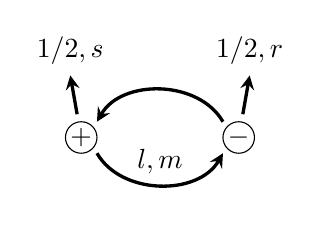
\begin{tikzpicture}[>=stealth]
    \draw (0, 0) circle [radius=0.2] node {$+$};
    \draw[very thick, ->] (100: 0.3) -- (100: 0.8) node [above] {$1/2, s$};
    \begin{scope}[xshift=2cm]
      \draw (0, 0) circle [radius=0.2] node {$-$};
      \draw[very thick, ->] (80: 0.3) -- (80: 0.8) node [above] {$1/2, r$};
    \end{scope}
    \draw[very thick, ->] (0.2, -0.2) to [out=-60, in =-120] (1.8, -0.2);
    \draw[very thick, ->] (1.8, 0.2) to [out=120, in =60] (0.2, 0.2);
    \draw (1, -0.3) node {$l, m$};
  \end{tikzpicture}
\end{center}

(電子と陽電子の合計)スピン$S$,射影$S_z$,相対運動量$\boldsymbol{p}$の状態$\ket{S, S_z}_{\boldsymbol{p}}$は,
スピン射影$s$で運動量$\boldsymbol{p}$の電子と,スピン射影$r:=S_z-s$で運動量$\boldsymbol{p}$の陽電子の線形結合で表せる:
\begin{align*}
  \ket{S, S_z}_{\boldsymbol{p}} &= \sum_s \Braket{ \frac{1}{2} \frac{1}{2}; s r | \frac{1}{2} \frac{1}{2}; S S_z} \Ket{\frac{1}{2}, s}_{\boldsymbol{p}} \Ket{\frac{1}{2}, r}_{-\boldsymbol{p}} \\
  &= \sum_s \Braket{ \frac{1}{2} \frac{1}{2}; s r | \frac{1}{2} \frac{1}{2}; S S_z}
  \frac{1}{\sqrt{2m}} \frac{1}{\sqrt{2m}} a_{\boldsymbol{p}}^{s\dagger} b_{-\boldsymbol{p}}^{r\dagger} \ket{0} .
\end{align*}

まず,$S$状態($l=0$)のポジトロニウムについて考える($m=0$なので$M=S_z$).
$\ket{^1S_0; 0}$は$J=M=0$, $S=S_z=0$なのでスピンはsinglet:
\begin{align}
  \ket{^1S_0; 0} = 2\sqrt{m} \int \frac{d^3p}{(2\pi)^3} \tilde{\psi}_{00}(\boldsymbol{p}) \frac{1}{\sqrt{2m}} \frac{1}{\sqrt{2m}}
  \frac{\ket{\boldsymbol{p} \uparrow, -\boldsymbol{p} \downarrow} - \ket{\boldsymbol{p} \downarrow, -\boldsymbol{p} \uparrow}}{\sqrt{2}} .
  \label{prob5_4a_1S_0;0}
\end{align}
$\ket{^3S_1; 0}$は$J=1$, $M=0$, $S=1$, $S_z=0$なのでスピンはtriplet:
\begin{align*}
  \ket{^3S_1; 0} = 2\sqrt{m} \int \frac{d^3p}{(2\pi)^3} \tilde{\psi}_{00}(\boldsymbol{p}) \frac{1}{\sqrt{2m}} \frac{1}{\sqrt{2m}}
  \frac{\ket{\boldsymbol{p} \uparrow, -\boldsymbol{p} \downarrow} + \ket{\boldsymbol{p} \downarrow, -\boldsymbol{p} \uparrow}}{\sqrt{2}} .
\end{align*}
$\ket{^3S_1; 1}$は$J=1$, $M=1$, $S=1$, $S_z=1$なのでスピンはtriplet:
\begin{align*}
  \ket{^3S_1; 1} = 2\sqrt{m} \int \frac{d^3p}{(2\pi)^3} \tilde{\psi}_{00}(\boldsymbol{p}) \frac{1}{\sqrt{2m}} \frac{1}{\sqrt{2m}} \ket{\boldsymbol{p} \uparrow, -\boldsymbol{p} \uparrow} .
\end{align*}
$\ket{^3S_1; -1}$は$J=1$, $M=-1$, $S=1$, $S_z=-1$なのでスピンはtriplet:
\begin{align*}
  \ket{^3S_1; -1} = 2\sqrt{m} \int \frac{d^3p}{(2\pi)^3} \tilde{\psi}_{00}(\boldsymbol{p}) \frac{1}{\sqrt{2m}} \frac{1}{\sqrt{2m}} \ket{\boldsymbol{p} \downarrow, -\boldsymbol{p} \downarrow} .
\end{align*}

\subsubsection{Sポジトロニウムの崩壊}
不変振幅$\mathcal{M}$の定義(4.73)に注意して,\eqref{prob5_4a_iM_cal}\eqref{prob5_4a_spinor}\eqref{prob5_4a_1S_0;0}から
\begin{align}
  \begin{split}
    i\mathcal{M}(^1S_0 \to 2\gamma) &= 2\sqrt{m} \int \frac{d^3p}{(2\pi)^3} \tilde{\psi}_{00}(\boldsymbol{p}) \frac{1}{2m}
    \frac{i\mathcal{M}(e^-_\uparrow e^+_\downarrow \to 2\gamma) - i\mathcal{M}(e^-_\downarrow e^+_\uparrow \to 2\gamma)}{\sqrt{2}} \\
    &= 2\sqrt{m} \int \frac{d^3p}{(2\pi)^3} \tilde{\psi}_{00}(\boldsymbol{p}) \frac{1}{2m} \left( -\frac{2e^2}{m} \right) (\boldsymbol{\epsilon}_1^\ast \times \boldsymbol{\epsilon}_2^\ast) \cdot \boldsymbol{k}
    \frac{ \eta^{\downarrow\dagger}\xi^\uparrow - \eta^{\uparrow\dagger}\xi^\downarrow}{\sqrt{2}} \\
    &= 2\sqrt{m} \int \frac{d^3p}{(2\pi)^3} \tilde{\psi}_{00}(\boldsymbol{p}) \frac{1}{2m} \left( -\frac{2e^2}{m} \right) (\boldsymbol{\epsilon}_1^\ast \times \boldsymbol{\epsilon}_2^\ast) \cdot \boldsymbol{k} \frac{-2}{\sqrt{2}} \\
    &= 2\sqrt{m} \int \frac{d^3p}{(2\pi)^3} \tilde{\psi}_{00}(\boldsymbol{p}) \frac{1}{2m} \left( -\frac{2e^2}{m} \right) (\boldsymbol{\epsilon}_1^\ast \times \boldsymbol{\epsilon}_2^\ast) \cdot \boldsymbol{k} \frac{-2}{\sqrt{2}} \\
    &= 2\sqrt{2} \frac{e^2}{m\sqrt{m}}  (\boldsymbol{\epsilon}_1^\ast \times \boldsymbol{\epsilon}_2^\ast) \cdot \boldsymbol{k} \int \frac{d^3p}{(2\pi)^3} \tilde{\psi}_{00}(\boldsymbol{p}) \\
    &= 2\sqrt{2} \frac{e^2}{m\sqrt{m}} (\boldsymbol{\epsilon}_1^\ast \times \boldsymbol{\epsilon}_2^\ast) \cdot \boldsymbol{k} \psi_{00}(0) .
  \end{split}
  \label{prob5_4a_1S_0_2hv}
\end{align}

(A.26)から
\[ \sum_\text{polarization} \epsilon^{\mu\ast}\epsilon^\nu \to -g^{\mu\nu} \]
なので,
\begin{align}
  \begin{split}
    \lvert (\boldsymbol{\epsilon}_1^\ast \times \boldsymbol{\epsilon}_2^\ast) \cdot \boldsymbol{k} \rvert^2
    &= \sum_\text{pol 1}\sum_\text{pol 2}\sum_{ijklmn} \epsilon^{ijk} \epsilon_1^{i\ast}\epsilon_2^{j\ast} k^k \epsilon^{lmn} \epsilon_1^l\epsilon_2^m k^n \\
    &\to \sum_{ijklmn} \epsilon^{ijk}\epsilon^{lmn} g^{il} g^{jm} k^k k^n \\
    &= \sum_{klmn} \epsilon^{lmk}\epsilon^{lmn} k^k k^n \\
    &= \sum_{lmn} \epsilon^{lmn}\epsilon^{lmn} k^n k^n \\
    &= 2\lvert\boldsymbol{k}\rvert^2 = 2E^2 \approx 2m^2
  \end{split}
  \label{prob5_4a_pol_sum}
\end{align}
を得る.

$n=1$の場合\footnote{換算質量は$m/2$なので,Bohr半径$a_0 = 2/\alpha m$}を考える.
\[ \psi_{100} = R_{10}(r) Y_{00}(\theta, \phi) = \frac{1}{\sqrt{4\pi}} \frac{2}{a_0{}^{3/2}} \exp \left( - \frac{r}{2a_0} \right) \]
なので,
\begin{align}
  \lvert \psi_{100}(0) \rvert^2 = \frac{m^3\alpha^3}{8\pi} . \label{prob5_4a_wf_100}
\end{align}
\eqref{prob5_4a_1S_0_2hv}\eqref{prob5_4a_pol_sum}\eqref{prob5_4a_wf_100}から
\begin{align}
  \sum_\text{polarization} \lvert \mathcal{M}(1^1S_0 \to 2\gamma) \rvert^2 &= 8 \frac{e^4}{m^3} 2m^2 \frac{m^3\alpha^3}{8\pi} = 32\pi m^2 \alpha^5 .
\end{align}
(4.86)から
\begin{align*}
  \Gamma(1^1S_0 \to 2\gamma) &= \frac{1}{2} \frac{1}{4m} \int \frac{d^3k_1}{(2\pi)^3}\frac{d^3k_2}{(2\pi)^3} \frac{1}{4E_1E_2} \lvert \mathcal{M}(^1S_0 \to 2\gamma) \rvert^2 (2\pi)^4 \mathop{\delta^{(4)}}(k_1+k_2-p_1-p_2) \\
  &= \frac{1}{8m} \int \frac{d^3k_1}{(2\pi)^2} \frac{1}{4\lvert \boldsymbol{k}_1 \rvert^2} 32\pi m^2 \alpha^5 \mathop\delta(2E_1 - 2m) \\
  &= \pi m\alpha^5 4\pi \int \frac{d\lvert \boldsymbol{k}_1 \rvert}{(2\pi)^2} \frac{1}{2} \mathop\delta(\lvert \boldsymbol{k}_1 \rvert - m) \\
  &= \frac{m\alpha^5}{2}
\end{align*}
(出てくる光子は区別できないので,$1/2$倍する).

\eqref{prob5_4a_1S_0_2hv}と同様に考えれば,
\begin{align*}
  \eta^{\uparrow\dagger}\xi^\uparrow = 0
  & , &
  \frac{\eta^{\uparrow\dagger}\xi^\downarrow + \eta^{\downarrow\dagger}\xi^\uparrow}{\sqrt{2}} = 0
  & , &
  \eta^{\downarrow\dagger}\xi^\downarrow = 0
\end{align*}
なので,$\mathcal{M}(^3S_1 \to 2\gamma) = 0$であることが分かる.
すなわち,スピン$1$の$1^3S$は2光子に崩壊しない.

\subsubsection{対消滅の不変振幅(1次)}
対消滅の不変振幅を運動量$p$の$1$次までの精度で求める.
\begin{align*}
  p_1^\mu  = (E, \boldsymbol{p})
  & , &
  p_2^\mu = (E, -\boldsymbol{p})
  & , &
  k_1^\mu = (E, \boldsymbol{k})
  & , &
  k_2^\mu = (E, -\boldsymbol{k})
  .
\end{align*}
光子の偏極は次のようにおく:
\begin{align*}
  \epsilon_{\pm}^\mu(k_1) = \epsilon_{1\pm}^\mu = (0, \boldsymbol{\epsilon}_1)
  & , &
  \boldsymbol{\epsilon}_1 \cdot \boldsymbol{k}_1 = 0
  & , &
  \epsilon_{\pm}^\mu(k_2) = \epsilon_{2\pm}^\mu = (0, \boldsymbol{\epsilon}_2)
  & , &
  \boldsymbol{\epsilon}_2 \cdot \boldsymbol{k}_2 = 0
  .
\end{align*}
スピノルは次のように近似される:
\begin{align}
  u(p_1) =
  \begin{pmatrix}
    \sqrt{\sigma \cdot p_1} \xi \\
    \sqrt{\overline\sigma \cdot p_1} \xi
  \end{pmatrix}
  \approx \sqrt{m}
  \begin{pmatrix}
    \left( 1 - \dfrac{\boldsymbol\sigma \cdot \boldsymbol{p}}{2m} \right) \xi \\[10pt]
    \left( 1 + \dfrac{\boldsymbol\sigma \cdot \boldsymbol{p}}{2m} \right) \xi
  \end{pmatrix}
  & , &
  v(p_2) =
  \begin{pmatrix}
    \sqrt{\sigma \cdot p_2} \eta \\
    -\sqrt{\overline\sigma \cdot p_2} \eta
  \end{pmatrix}
  \approx \sqrt{m}
  \begin{pmatrix}
    \left( 1 + \dfrac{\boldsymbol\sigma \cdot \boldsymbol{p}}{2m} \right) \eta \\[10pt]
    -\left( 1 - \dfrac{\boldsymbol\sigma \cdot \boldsymbol{p}}{2m} \right) \eta
  \end{pmatrix}
  . \label{prob5_4b_spinor_approx}
\end{align}
さらに,
\begin{align*}
  p_1 \cdot k_1 &= E^2 - \boldsymbol{p} \cdot \boldsymbol{k} \approx m^2 - \boldsymbol{p} \cdot \boldsymbol{k}, \\
  p_1 \cdot k_2 &= E^2 + \boldsymbol{p} \cdot \boldsymbol{k} \approx m^2 + \boldsymbol{p} \cdot \boldsymbol{k}, \\
  (p_1 \cdot k_1)(p_1 \cdot k_2) &\approx m^4 .
\end{align*}

Dirac方程式から次を得る:
\begin{align*}
  (\slashed{p}_1 + m) \slashed{\epsilon}_1^\ast u(p_1) &= 2 (p_1 \cdot \epsilon_1^\ast) u(p_1) - \slashed{\epsilon}_1^\ast (\slashed{p}_1 - m) u(p_1) = 2 (p_1 \cdot \epsilon_1^\ast) u(p_1) , \\
  (\slashed{p}_1 + m) \slashed{\epsilon}_2^\ast u(p_1) &= 2 (p_1 \cdot \epsilon_2^\ast) u(p_1) - \slashed{\epsilon}_2^\ast (\slashed{p}_1 - m) u(p_1) = 2 (p_1 \cdot \epsilon_2^\ast) u(p_1) .
\end{align*}
従って,不変振幅は
\begin{align}
  \begin{split}
    i\mathcal{M} &= -ie^2 \overline{v}(p_2) \left[ \slashed{\epsilon}_2^\ast \frac{\slashed{p}_1 - \slashed{k}_1 + m}{(p_1 - k_1)^2 - m^2} \slashed{\epsilon}_1^\ast
    + \slashed{\epsilon}_1^\ast \frac{\slashed{p}_1 - \slashed{k}_2 + m}{(p_1 - k_2)^2 - m^2} \slashed{\epsilon}_2^\ast \right] u(p_1) \\
    %
    &= -ie^2 \overline{v}(p_2) \left[ \slashed{\epsilon}_2^\ast \frac{-\slashed{p}_1 + \slashed{k}_1 - m}{2p_1 \cdot k_1} \slashed{\epsilon}_1^\ast
    + \slashed{\epsilon}_1^\ast \frac{-\slashed{p}_1 + \slashed{k}_2 - m}{2p_1 \cdot k_2} \slashed{\epsilon}_2^\ast \right] u(p_1) \\
    %
    &= -i\frac{e^2}{2} \overline{v}(p_2) \left[
    \frac{\slashed{\epsilon}_2^\ast\slashed{k}_1\slashed{\epsilon}_1^\ast - 2(p_1 \cdot \epsilon_1^\ast)\slashed{\epsilon}_2^\ast}{m^2 - \boldsymbol{p} \cdot \boldsymbol{k}}
    + \frac{\slashed{\epsilon}_1^\ast\slashed{k}_2\slashed{\epsilon}_2^\ast - 2(p_1 \cdot \epsilon_2^\ast)\slashed{\epsilon}_1^\ast}{m^2 + \boldsymbol{p} \cdot \boldsymbol{k}}
    \right] u(p_1) \\
    %
    &= -i\frac{e^2}{2m^4} \overline{v}(p_2) \left[
    (m^2 + \boldsymbol{p} \cdot \boldsymbol{k})(\slashed{\epsilon}_2^\ast\slashed{k}_1\slashed{\epsilon}_1^\ast - 2(p_1 \cdot \epsilon_1^\ast)\slashed{\epsilon}_2^\ast)
    + (m^2 - \boldsymbol{p} \cdot \boldsymbol{k})(\slashed{\epsilon}_1^\ast\slashed{k}_2\slashed{\epsilon}_2^\ast - 2(p_1 \cdot \epsilon_2^\ast)\slashed{\epsilon}_1^\ast)
    \right] u(p_1)
  \end{split}
  \label{prob5_4b_iM}
\end{align}
となる.$[\cdots]$を計算するが,まず次の式を示しておく:
\begin{align*}
  \slashed{a}\slashed{b}\slashed{c} &= a_\mu b_\nu c_\rho
  \begin{pmatrix}
    0 & \sigma^\mu \\
    \overline{\sigma}^\mu & 0
  \end{pmatrix}
  \begin{pmatrix}
    0 & \sigma^\nu \\
    \overline{\sigma}^\nu & 0
  \end{pmatrix}
  \begin{pmatrix}
    0 & \sigma^\rho \\
    \overline{\sigma}^\rho & 0
  \end{pmatrix}
  \\
  &= a_\mu b_\nu c_\rho
  \begin{pmatrix}
    0 & \sigma^\mu \overline{\sigma}^\nu \sigma^\rho \\
    \overline{\sigma}^\mu \sigma^\nu \overline{\sigma}^\rho & 0
  \end{pmatrix}
  \\
  &=
  \begin{pmatrix}
    0 & (a \cdot \sigma)(b \cdot \overline\sigma)(c \cdot \sigma) \\
    (a \cdot \overline\sigma)(b \cdot \sigma)(c \cdot \overline\sigma) & 0
  \end{pmatrix}
  .
\end{align*}

\eqref{prob5_4b_iM}の$[\cdots]$のうち$m^2$と1つのガンマ行列を含む項は
\begin{align*}
  & -2m^2 (p_1 \cdot \epsilon_1^\ast) \slashed{\epsilon}_2^\ast -2m^2 (p_1 \cdot \epsilon_2^\ast) \slashed{\epsilon}_1^\ast  \\
  &= -2m^2 (p_1 \cdot \epsilon_1^\ast)
  \begin{pmatrix}
    0 & \epsilon_2^\ast \cdot \sigma \\
    \epsilon_2^\ast \cdot \overline\sigma & 0
  \end{pmatrix}
  -2m^2 (p_1 \cdot \epsilon_2^\ast)
  \begin{pmatrix}
    0 & \epsilon_1^\ast \cdot \sigma \\
    \epsilon_1^\ast \cdot \overline\sigma & 0
  \end{pmatrix}
  \\
  %
  &= -2m^2 (\boldsymbol{p} \cdot \boldsymbol{\epsilon}_1^\ast)
  \begin{pmatrix}
    0 & \boldsymbol{\epsilon}_2^\ast \cdot \boldsymbol\sigma \\
    -\boldsymbol{\epsilon}_2^\ast \cdot \boldsymbol\sigma & 0
  \end{pmatrix}
  -2m^2 (\boldsymbol{p} \cdot \boldsymbol{\epsilon}_2^\ast)
  \begin{pmatrix}
    0 & \boldsymbol{\epsilon}_1^\ast \cdot \boldsymbol\sigma \\
    -\boldsymbol{\epsilon}_1^\ast \cdot \boldsymbol\sigma & 0
  \end{pmatrix}
  \\
  %
  &= -2m^2
  \begin{pmatrix}
    0 & (\boldsymbol{p} \cdot \boldsymbol{\epsilon}_1^\ast)(\boldsymbol{\epsilon}_2^\ast \cdot \boldsymbol\sigma)
    + (\boldsymbol{p} \cdot \boldsymbol{\epsilon}_2^\ast)(\boldsymbol{\epsilon}_1^\ast \cdot \boldsymbol\sigma)
    \\
    -(\boldsymbol{p} \cdot \boldsymbol{\epsilon}_1^\ast)(\boldsymbol{\epsilon}_2^\ast \cdot \boldsymbol\sigma)
    - (\boldsymbol{p} \cdot \boldsymbol{\epsilon}_2^\ast)(\boldsymbol{\epsilon}_1^\ast \cdot \boldsymbol\sigma)
    & 0
  \end{pmatrix}
  \\
  & =:
  \begin{pmatrix}
    0 & -2m^2 A \\
    2m^2 A & 0
  \end{pmatrix}
  .
\end{align*}

\eqref{prob5_4b_iM}の$[\cdots]$のうち$m^2$と3つのガンマ行列を含む項は
\begin{align*}
  & m^2\left[ \slashed{\epsilon}_2^\ast\slashed{k}_1\slashed{\epsilon}_1^\ast + \slashed{\epsilon}_1^\ast\slashed{k}_2\slashed{\epsilon}_2^\ast \right] \\
  &\quad = m^2
  \begin{pmatrix}
    0 & (\epsilon_2^\ast \cdot \sigma)(k_1 \cdot \overline\sigma)(\epsilon_1^\ast \cdot \sigma) \\
    (\epsilon_2^\ast \cdot \overline\sigma)(k_1 \cdot \sigma)(\epsilon_1^\ast \cdot \overline\sigma) & 0
  \end{pmatrix}
  \\
  & \quad + m^2
  \begin{pmatrix}
    0 & (\epsilon_1^\ast \cdot \sigma)(k_2 \cdot \overline\sigma)(\epsilon_2^\ast \cdot \sigma) \\
    (\epsilon_1^\ast \cdot \overline\sigma)(k_2 \cdot \sigma)(\epsilon_2^\ast \cdot \overline\sigma) & 0
  \end{pmatrix}
  \\
  &\quad = m^2
  \begin{pmatrix}
    0 & (\boldsymbol{\epsilon}_2^\ast \cdot \boldsymbol\sigma)(k_1 \cdot \overline\sigma)(\boldsymbol{\epsilon}_1^\ast \cdot \boldsymbol\sigma) \\
    (\boldsymbol{\epsilon}_2^\ast \cdot \boldsymbol\sigma)(k_1 \cdot \sigma)(\boldsymbol{\epsilon}_1^\ast \cdot \boldsymbol\sigma) & 0
  \end{pmatrix}
  \\
  & \quad + m^2
  \begin{pmatrix}
    0 & (\boldsymbol{\epsilon}_1^\ast \cdot \boldsymbol\sigma)(k_2 \cdot \overline\sigma)(\boldsymbol{\epsilon}_2^\ast \cdot \boldsymbol\sigma) \\
    (\boldsymbol{\epsilon}_1^\ast \cdot \boldsymbol\sigma)(k_2 \cdot \sigma)(\boldsymbol{\epsilon}_2^\ast \cdot \boldsymbol\sigma) & 0
  \end{pmatrix}
  \\
  &=:
  \begin{pmatrix}
    0 & m^2\overline{B}_+ \\
    m^2 B_+ & 0
  \end{pmatrix}
  .
\end{align*}

\eqref{prob5_4b_iM}の$[\cdots]$のうち$\boldsymbol{p}\cdot\boldsymbol{k}$と3つのガンマ行列を含む項は
\begin{align*}
  & \boldsymbol{p} \cdot \boldsymbol{k}\left[ \slashed{\epsilon}_2^\ast\slashed{k}_1\slashed{\epsilon}_1^\ast - \slashed{\epsilon}_1^\ast\slashed{k}_2\slashed{\epsilon}_2^\ast \right] \\
  &\quad = \boldsymbol{p} \cdot \boldsymbol{k}
  \begin{pmatrix}
    0 & (\epsilon_2^\ast \cdot \sigma)(k_1 \cdot \overline\sigma)(\epsilon_1^\ast \cdot \sigma) \\
    (\epsilon_2^\ast \cdot \overline\sigma)(k_1 \cdot \sigma)(\epsilon_1^\ast \cdot \overline\sigma) & 0
  \end{pmatrix}
  \\
  & \quad - \boldsymbol{p} \cdot \boldsymbol{k}
  \begin{pmatrix}
    0 & (\epsilon_1^\ast \cdot \sigma)(k_2 \cdot \overline\sigma)(\epsilon_2^\ast \cdot \sigma) \\
    (\epsilon_1^\ast \cdot \overline\sigma)(k_2 \cdot \sigma)(\epsilon_2^\ast \cdot \overline\sigma) & 0
  \end{pmatrix}
  \\
  &\quad = \boldsymbol{p} \cdot \boldsymbol{k}
  \begin{pmatrix}
    0 & (\boldsymbol{\epsilon}_2^\ast \cdot \boldsymbol\sigma)(k_1 \cdot \overline\sigma)(\boldsymbol{\epsilon}_1^\ast \cdot \boldsymbol\sigma) \\
    (\boldsymbol{\epsilon}_2^\ast \cdot \boldsymbol\sigma)(k_1 \cdot \sigma)(\boldsymbol{\epsilon}_1^\ast \cdot \boldsymbol\sigma) & 0
  \end{pmatrix}
  \\
  & \quad - \boldsymbol{p} \cdot \boldsymbol{k}
  \begin{pmatrix}
    0 & (\boldsymbol{\epsilon}_1^\ast \cdot \boldsymbol\sigma)(k_2 \cdot \overline\sigma)(\boldsymbol{\epsilon}_2^\ast \cdot \boldsymbol\sigma) \\
    (\boldsymbol{\epsilon}_1^\ast \cdot \boldsymbol\sigma)(k_2 \cdot \sigma)(\boldsymbol{\epsilon}_2^\ast \cdot \boldsymbol\sigma) & 0
  \end{pmatrix}
  \\
  &=:
  \begin{pmatrix}
    0 & -(\boldsymbol{p} \cdot \boldsymbol{k})\overline{B}_- \\
    -(\boldsymbol{p} \cdot \boldsymbol{k}) B_- & 0
  \end{pmatrix}
  .
\end{align*}

\eqref{prob5_4b_iM}の残りの項は運動量の$2$乗なので無視する:
\begin{align*}
  & -2 (\boldsymbol{p}\cdot\boldsymbol{k}) (p_1 \cdot \epsilon_1^\ast) \slashed{\epsilon}_2^\ast + 2(\boldsymbol{p}\cdot\boldsymbol{k}) (p_1 \cdot \epsilon_2^\ast) \slashed{\epsilon}_1^\ast \\
  &= -2(\boldsymbol{p}\cdot\boldsymbol{k}) (p_1 \cdot \epsilon_1^\ast)
  \begin{pmatrix}
    0 & \epsilon_2^\ast \cdot \sigma \\
    \epsilon_2^\ast \cdot \overline\sigma & 0
  \end{pmatrix}
  + 2(\boldsymbol{p}\cdot\boldsymbol{k}) (p_1 \cdot \epsilon_2^\ast)
  \begin{pmatrix}
    0 & \epsilon_1^\ast \cdot \sigma \\
    \epsilon_1^\ast \cdot \overline\sigma & 0
  \end{pmatrix}
  \\
  %
  &= -2(\boldsymbol{p}\cdot\boldsymbol{k}) (\boldsymbol{p} \cdot \boldsymbol{\epsilon}_1^\ast)
  \begin{pmatrix}
    0 & \boldsymbol{\epsilon}_2^\ast \cdot \boldsymbol\sigma \\
    -\boldsymbol{\epsilon}_2^\ast \cdot \boldsymbol\sigma & 0
  \end{pmatrix}
  + 2(\boldsymbol{p}\cdot\boldsymbol{k}) (\boldsymbol{p} \cdot \boldsymbol{\epsilon}_2^\ast)
  \begin{pmatrix}
    0 & \boldsymbol{\epsilon}_1^\ast \cdot \boldsymbol\sigma \\
    -\boldsymbol{\epsilon}_1^\ast \cdot \boldsymbol\sigma & 0
  \end{pmatrix}
  \\
  %
  &= -2(\boldsymbol{p}\cdot\boldsymbol{k})
  \begin{pmatrix}
    0 & (\boldsymbol{p} \cdot \boldsymbol{\epsilon}_1^\ast)(\boldsymbol{\epsilon}_2^\ast \cdot \boldsymbol\sigma)
    - (\boldsymbol{p} \cdot \boldsymbol{\epsilon}_2^\ast)(\boldsymbol{\epsilon}_1^\ast \cdot \boldsymbol\sigma)
    \\
    -(\boldsymbol{p} \cdot \boldsymbol{\epsilon}_1^\ast)(\boldsymbol{\epsilon}_2^\ast \cdot \boldsymbol\sigma)
    + (\boldsymbol{p} \cdot \boldsymbol{\epsilon}_2^\ast)(\boldsymbol{\epsilon}_1^\ast \cdot \boldsymbol\sigma)
    & 0
  \end{pmatrix}
  \\
  &\approx 0 .
\end{align*}

以上から
\begin{align}
  i\mathcal{M}= -i\frac{e^2}{2m^4} \overline{v}(p_2)
  \begin{pmatrix}
    0 & -2m^2A + m^2\overline{B}_+ - (\boldsymbol{p}\cdot\boldsymbol{k}) \overline{B}_- \\
    2m^2A + m^2B_+ - (\boldsymbol{p}\cdot\boldsymbol{k}) B_- & 0
  \end{pmatrix}
  u(p_1) \label{prob5_4b_iM_AB}
\end{align}
となる.各項の定義は
\begin{align}
  \begin{split}
    A &= (\boldsymbol{p} \cdot \boldsymbol{\epsilon}_1^\ast)(\boldsymbol{\epsilon}_2^\ast \cdot \boldsymbol\sigma)
    + (\boldsymbol{p} \cdot \boldsymbol{\epsilon}_2^\ast)(\boldsymbol{\epsilon}_1^\ast \cdot \boldsymbol\sigma) \\
    B_\pm &= (\boldsymbol{\epsilon}_1^\ast \cdot \boldsymbol\sigma)(k_2 \cdot \sigma)(\boldsymbol{\epsilon}_2^\ast \cdot \boldsymbol\sigma)
    \pm (\boldsymbol{\epsilon}_2^\ast \cdot \boldsymbol\sigma)(k_1 \cdot \sigma)(\boldsymbol{\epsilon}_1^\ast \cdot \boldsymbol\sigma) \\
    \overline{B}_\pm &= (\boldsymbol{\epsilon}_1^\ast \cdot \boldsymbol\sigma)(k_2 \cdot \overline\sigma)(\boldsymbol{\epsilon}_2^\ast \cdot \boldsymbol\sigma)
    \pm (\boldsymbol{\epsilon}_2^\ast \cdot \boldsymbol\sigma)(k_1 \cdot \overline\sigma)(\boldsymbol{\epsilon}_1^\ast \cdot \boldsymbol\sigma)
    .
  \end{split}
  \label{prob5_4b_AB_def}
\end{align}

$(\boldsymbol\sigma \cdot \boldsymbol{a}) (\boldsymbol\sigma \cdot \boldsymbol{b}) = \boldsymbol{a} \cdot \boldsymbol{b} + i \boldsymbol\sigma \cdot (\boldsymbol{a} \times \boldsymbol{b})$から
\begin{align*}
  (\boldsymbol{\epsilon}_1^\ast \cdot \boldsymbol\sigma)(\boldsymbol{k}\cdot\boldsymbol\sigma)(\boldsymbol{\epsilon}_2^\ast \cdot \boldsymbol\sigma)
  &= [\boldsymbol{\epsilon}_1^\ast \cdot \boldsymbol{k} + i \boldsymbol\sigma \cdot (\boldsymbol{\epsilon}_1^\ast \times \boldsymbol{k})](\boldsymbol{\epsilon}_2^\ast \cdot \boldsymbol\sigma) \\
  &= i \boldsymbol\sigma \cdot (\boldsymbol{\epsilon}_1^\ast \times \boldsymbol{k})(\boldsymbol{\epsilon}_2^\ast \cdot \boldsymbol\sigma) \\
  &= i (\boldsymbol{\epsilon}_1^\ast \times \boldsymbol{k}) \cdot \boldsymbol{\epsilon}_2^\ast - \boldsymbol\sigma \cdot [(\boldsymbol{\epsilon}_1^\ast \times \boldsymbol{k}) \times \boldsymbol{\epsilon}_2^\ast] \\
  &= i (\boldsymbol{\epsilon}_2^\ast \times \boldsymbol{\epsilon}_1^\ast) \cdot \boldsymbol{k} - \boldsymbol\sigma \cdot [(\boldsymbol{\epsilon}_1^\ast \cdot \boldsymbol{\epsilon}_2^\ast) \boldsymbol{k} - (\boldsymbol{k} \cdot \boldsymbol{\epsilon}_2^\ast) \boldsymbol{\epsilon}_1^\ast] \\
  &= - i (\boldsymbol{\epsilon}_1^\ast \times \boldsymbol{\epsilon}_2^\ast) \cdot \boldsymbol{k}
  - (\boldsymbol\sigma \cdot \boldsymbol{k})(\boldsymbol{\epsilon}_1^\ast \cdot \boldsymbol{\epsilon}_2^\ast) \\
  %
  (\boldsymbol{\epsilon}_2^\ast \cdot \boldsymbol\sigma)(\boldsymbol{k}\cdot\boldsymbol\sigma)(\boldsymbol{\epsilon}_1^\ast \cdot \boldsymbol\sigma)
  &=  i (\boldsymbol{\epsilon}_1^\ast \times \boldsymbol{\epsilon}_2^\ast) \cdot \boldsymbol{k}
  - (\boldsymbol\sigma \cdot \boldsymbol{k})(\boldsymbol{\epsilon}_1^\ast \cdot \boldsymbol{\epsilon}_2^\ast) \\
  %
  (\boldsymbol{\epsilon}_1^\ast \cdot \boldsymbol\sigma)(\boldsymbol{\epsilon}_2^\ast \cdot \boldsymbol\sigma)
  + (\boldsymbol{\epsilon}_2^\ast \cdot \boldsymbol\sigma)(\boldsymbol{\epsilon}_1^\ast \cdot \boldsymbol\sigma)
  &= 2 \boldsymbol{\epsilon}_1^\ast \cdot \boldsymbol{\epsilon}_2^\ast
\end{align*}
となる.従って,
\begin{align}
  \begin{split}
    \overline{B}_+ - B_+ &= (\boldsymbol{\epsilon}_1^\ast \cdot \boldsymbol\sigma)(k_2 \cdot \overline\sigma)(\boldsymbol{\epsilon}_2^\ast \cdot \boldsymbol\sigma)
    + (\boldsymbol{\epsilon}_2^\ast \cdot \boldsymbol\sigma)(k_1 \cdot \overline\sigma)(\boldsymbol{\epsilon}_1^\ast \cdot \boldsymbol\sigma) \\
    &- (\boldsymbol{\epsilon}_1^\ast \cdot \boldsymbol\sigma)(k_2 \cdot \sigma)(\boldsymbol{\epsilon}_2^\ast \cdot \boldsymbol\sigma)
    - (\boldsymbol{\epsilon}_2^\ast \cdot \boldsymbol\sigma)(k_1 \cdot \sigma)(\boldsymbol{\epsilon}_1^\ast \cdot \boldsymbol\sigma) \\
    &= (\boldsymbol{\epsilon}_1^\ast \cdot \boldsymbol\sigma)(k_2 \cdot (\overline\sigma - \sigma))(\boldsymbol{\epsilon}_2^\ast \cdot \boldsymbol\sigma)
    + (\boldsymbol{\epsilon}_2^\ast \cdot \boldsymbol\sigma)(k_1 \cdot (\overline\sigma - \sigma))(\boldsymbol{\epsilon}_1^\ast \cdot \boldsymbol\sigma) \\
    &= -2(\boldsymbol{\epsilon}_1^\ast \cdot \boldsymbol\sigma)(\boldsymbol{k}\cdot\boldsymbol\sigma)(\boldsymbol{\epsilon}_2^\ast \cdot \boldsymbol\sigma)
    + 2(\boldsymbol{\epsilon}_2^\ast \cdot \boldsymbol\sigma)(\boldsymbol{k}\cdot\boldsymbol\sigma)(\boldsymbol{\epsilon}_1^\ast \cdot \boldsymbol\sigma) \\
    &= 4i (\boldsymbol{\epsilon}_1^\ast \times \boldsymbol{\epsilon}_2^\ast) \cdot \boldsymbol{k} , \\
    %
    B_- - \overline{B}_- &= (\boldsymbol{\epsilon}_1^\ast \cdot \boldsymbol\sigma)(k_2 \cdot \sigma)(\boldsymbol{\epsilon}_2^\ast \cdot \boldsymbol\sigma)
    - (\boldsymbol{\epsilon}_2^\ast \cdot \boldsymbol\sigma)(k_1 \cdot \sigma)(\boldsymbol{\epsilon}_1^\ast \cdot \boldsymbol\sigma) \\
    &- (\boldsymbol{\epsilon}_1^\ast \cdot \boldsymbol\sigma)(k_2 \cdot \overline\sigma)(\boldsymbol{\epsilon}_2^\ast \cdot \boldsymbol\sigma)
    + (\boldsymbol{\epsilon}_2^\ast \cdot \boldsymbol\sigma)(k_1 \cdot \overline\sigma)(\boldsymbol{\epsilon}_1^\ast \cdot \boldsymbol\sigma) \\
    &= (\boldsymbol{\epsilon}_1^\ast \cdot \boldsymbol\sigma)(k_2 \cdot (\sigma - \overline\sigma ))(\boldsymbol{\epsilon}_2^\ast \cdot \boldsymbol\sigma)
    - (\boldsymbol{\epsilon}_2^\ast \cdot \boldsymbol\sigma)(k_1 \cdot (\sigma - \overline\sigma))(\boldsymbol{\epsilon}_1^\ast \cdot \boldsymbol\sigma) \\
    &= 2(\boldsymbol{\epsilon}_1^\ast \cdot \boldsymbol\sigma)(\boldsymbol{k}\cdot\boldsymbol\sigma)(\boldsymbol{\epsilon}_2^\ast \cdot \boldsymbol\sigma)
    + 2(\boldsymbol{\epsilon}_2^\ast \cdot \boldsymbol\sigma)(\boldsymbol{k}\cdot\boldsymbol\sigma)(\boldsymbol{\epsilon}_1^\ast \cdot \boldsymbol\sigma) \\
    &= -4(\boldsymbol\sigma \cdot \boldsymbol{k})(\boldsymbol{\epsilon}_1^\ast \cdot \boldsymbol{\epsilon}_2^\ast) , \\
    %
    B_+ + \overline{B}_+ &= (\boldsymbol{\epsilon}_1^\ast \cdot \boldsymbol\sigma)(k_2 \cdot \sigma)(\boldsymbol{\epsilon}_2^\ast \cdot \boldsymbol\sigma)
    + (\boldsymbol{\epsilon}_2^\ast \cdot \boldsymbol\sigma)(k_1 \cdot \sigma)(\boldsymbol{\epsilon}_1^\ast \cdot \boldsymbol\sigma) \\
    &+ (\boldsymbol{\epsilon}_1^\ast \cdot \boldsymbol\sigma)(k_2 \cdot \overline\sigma)(\boldsymbol{\epsilon}_2^\ast \cdot \boldsymbol\sigma)
    + (\boldsymbol{\epsilon}_2^\ast \cdot \boldsymbol\sigma)(k_1 \cdot \overline\sigma)(\boldsymbol{\epsilon}_1^\ast \cdot \boldsymbol\sigma) \\
    &= 2E(\boldsymbol{\epsilon}_1^\ast \cdot \boldsymbol\sigma)(\boldsymbol{\epsilon}_2^\ast \cdot \boldsymbol\sigma) + 2E(\boldsymbol{\epsilon}_2^\ast \cdot \boldsymbol\sigma)(\boldsymbol{\epsilon}_1^\ast \cdot \boldsymbol\sigma) \\
    &\approx 2m (\boldsymbol{\epsilon}_1^\ast \cdot \boldsymbol\sigma)(\boldsymbol{\epsilon}_2^\ast \cdot \boldsymbol\sigma) + 2m(\boldsymbol{\epsilon}_2^\ast \cdot \boldsymbol\sigma)(\boldsymbol{\epsilon}_1^\ast \cdot \boldsymbol\sigma) \\
    &= 4m \boldsymbol{\epsilon}_1^\ast \cdot \boldsymbol{\epsilon}_2^\ast .
  \end{split}
  \label{prob5_4b_BBB}
\end{align}

\eqref{prob5_4b_iM_AB}に\eqref{prob5_4b_spinor_approx}を代入して,\eqref{prob5_4b_BBB}を使えば,
\begin{align*}
  & i\mathcal{M}(e^-_se^+_r \to 2\gamma) \\
  &= -i\frac{e^2}{2m^4} \overline{v}(p_2)
  \begin{pmatrix}
    0 & -2m^2A + m^2\overline{B}_+ - (\boldsymbol{p}\cdot\boldsymbol{k}) \overline{B}_- \\
    2m^2A + m^2B_+ - (\boldsymbol{p}\cdot\boldsymbol{k}) B_- & 0
  \end{pmatrix}
  u(p_1) \\
  %
  &= -i\frac{e^2}{2m^3}
  \begin{pmatrix}
    \eta^{r\dagger}
    \left( 1 + \dfrac{\boldsymbol\sigma \cdot \boldsymbol{p}}{2m} \right) & - \eta^{r\dagger} \left( 1 - \dfrac{\boldsymbol\sigma \cdot \boldsymbol{p}}{2m} \right)
  \end{pmatrix}
  \begin{pmatrix}
    0 & 1 \\
    1 & 0
  \end{pmatrix}
  \\
  & \quad \times
  \begin{pmatrix}
    0 & -2m^2A + m^2\overline{B}_+ - (\boldsymbol{p}\cdot\boldsymbol{k}) \overline{B}_- \\
    2m^2A + m^2B_+ - (\boldsymbol{p}\cdot\boldsymbol{k}) B_- & 0
  \end{pmatrix}
  \begin{pmatrix}
    \left( 1 - \dfrac{\boldsymbol\sigma \cdot \boldsymbol{p}}{2m} \right) \xi^s \\[10pt]
    \left( 1 + \dfrac{\boldsymbol\sigma \cdot \boldsymbol{p}}{2m} \right) \xi^s
  \end{pmatrix}
  \\
  %
  & = i\frac{e^2}{2m^3} \eta^{r\dagger} \left( 1 - \dfrac{\boldsymbol\sigma \cdot \boldsymbol{p}}{2m} \right)
  \left[ -2m^2A + m^2\overline{B}_+ - (\boldsymbol{p}\cdot\boldsymbol{k}) \overline{B}_- \right]
  \left( 1 + \dfrac{\boldsymbol\sigma \cdot \boldsymbol{p}}{2m} \right) \xi^s \\
  &\quad -i\frac{e^2}{2m^3} \eta^{r\dagger} \left( 1 + \dfrac{\boldsymbol\sigma \cdot \boldsymbol{p}}{2m} \right)
  \left[ 2m^2A + m^2B_+ - (\boldsymbol{p}\cdot\boldsymbol{k}) B_- \right]
  \left( 1 - \dfrac{\boldsymbol\sigma \cdot \boldsymbol{p}}{2m} \right) \xi^s \\
  \\
  %
  & \approx i\frac{e^2}{2m^3} \eta^{r\dagger}
  \left\{ -2m^2A + m^2\overline{B}_+ - (\boldsymbol{p}\cdot\boldsymbol{k}) \overline{B}_- + \frac{m}{2} [\overline{B}_+, \boldsymbol\sigma \cdot \boldsymbol{p}] \right\}
  \xi^s \\
  & \quad -i\frac{e^2}{2m^3} \eta^{r\dagger}
  \left\{ 2m^2A + m^2B_+ - (\boldsymbol{p}\cdot\boldsymbol{k}) B_- - \frac{m}{2} [B_+, \boldsymbol\sigma \cdot \boldsymbol{p}] \right\}
  \xi^s \\
  &= i\frac{e^2}{2m^3} \eta^{r\dagger}
  \left\{ -4m^2A + m^2(\overline{B}_+ - B_+) + (\boldsymbol{p}\cdot\boldsymbol{k}) (B_- - \overline{B}_-) + \frac{m}{2} [B_+ + \overline{B}_+, \boldsymbol\sigma \cdot \boldsymbol{p}] \right\}
  \xi^s \\
  &= -i \frac{2e^2}{m} \eta^{r\dagger} \left[ (\boldsymbol{p} \cdot \boldsymbol{\epsilon}_1^\ast)(\boldsymbol{\epsilon}_2^\ast \cdot \boldsymbol\sigma)
  + (\boldsymbol{p} \cdot \boldsymbol{\epsilon}_2^\ast)(\boldsymbol{\epsilon}_1^\ast \cdot \boldsymbol\sigma)
  - i (\boldsymbol{\epsilon}_1^\ast \times \boldsymbol{\epsilon}_2^\ast) \cdot \boldsymbol{k}
  + \frac{1}{m^2} (\boldsymbol{p}\cdot\boldsymbol{k})(\boldsymbol\sigma \cdot \boldsymbol{k})(\boldsymbol{\epsilon}_1^\ast \cdot \boldsymbol{\epsilon}_2^\ast)
  \right] \xi^s
\end{align*}
となる.

ここで,
\begin{align}
  i\mathcal{M}^{(1)j} = -i \frac{2e^2}{m} \eta^{r\dagger} \left[ \epsilon_1^{j\ast} (\boldsymbol{\epsilon}_2^\ast \cdot \boldsymbol\sigma)
  + \epsilon_2^{j\ast} (\boldsymbol{\epsilon}_1^\ast \cdot \boldsymbol\sigma)
  + \frac{k^j}{m^2} (\boldsymbol\sigma \cdot \boldsymbol{k})(\boldsymbol{\epsilon}_1^\ast \cdot \boldsymbol{\epsilon}_2^\ast)
  \right] \xi^s
  \label{prob5_4b_iM_1_def}
\end{align}
とおけば,
\begin{align}
  & i\mathcal{M}(e^-_se^+_r \to 2\gamma) = i\mathcal{M}^{(0)} + \sum_j p^j i\mathcal{M}^{(1)j} \label{prob5_4b_iM_01}
\end{align}
とかける.

\subsubsection{$^3P_0$ポジトロニウムの構成}
$\ket{^3P_0;0}$は\eqref{prob5_4a_Ps_wf}で$S=1$, $l=1$, $J=0$, $M=0$なので
\begin{align*}
  \ket{^3P_0;0} &= \sqrt{2M} \int \frac{d^3p}{(2\pi)^3} \sum_{m=-1}^1
  \braket{1,1; m,-m | 1,1; 00} \tilde{\psi}_{1,m} \frac{1}{\sqrt{2m}}\frac{1}{\sqrt{2m}} \ket{1, -m} \\
  &= \frac{1}{\sqrt{3m}} \int \frac{d^3p}{(2\pi)^3} \left[ \tilde{\psi}_{11} \ket{\downarrow\downarrow}
  - \tilde{\psi}_{10} \frac{\ket{\uparrow\downarrow} + \ket{\downarrow\uparrow}}{\sqrt{2}} + \tilde{\psi}_{1,-1} \ket{\uparrow\uparrow} \right]
\end{align*}
となる.ここで
\begin{align}
  \tilde{\psi}^1 = \frac{\tilde{\psi}_{1,-1} - \tilde{\psi}_{1,1}}{\sqrt{2}} & , &
  \tilde{\psi}^2 = i\frac{\tilde{\psi}_{1,-1} + \tilde{\psi}_{1,1}}{\sqrt{2}} & , &
  \tilde{\psi}^3 = \tilde{\psi}_{1,0}
  \label{prob5_4b_wave_func_conv}
\end{align}
とおけば,
\begin{align*}
  \ket{^3P_0;0} &= \frac{1}{\sqrt{6m}} \int \frac{d^3p}{(2\pi)^3}
  \left[ \tilde{\psi}^1  (\ket{\uparrow\uparrow} - \ket{\downarrow\downarrow})
  - i \tilde{\psi}^2  (\ket{\uparrow\uparrow} + \ket{\downarrow\downarrow})
  - \tilde{\psi}^3 (\ket{\uparrow\downarrow} + \ket{\downarrow\uparrow}) \right]
\end{align*}
となる.

\subsubsection{$2^3P_0$ポジトロニウムの崩壊}
$n=2$の場合を考える.
\begin{align*}
  \psi^1(\boldsymbol{x}) &= \frac{1}{4\sqrt{2\pi}} \frac{1}{a_0{}^{5/2}} x \exp\left( -\frac{r}{2a_0} \right) \\
  \psi^2(\boldsymbol{x}) &= \frac{1}{4\sqrt{2\pi}} \frac{1}{a_0{}^{5/2}} y \exp\left( -\frac{r}{2a_0} \right) \\
  \psi^3(\boldsymbol{x}) &= \frac{1}{4\sqrt{2\pi}} \frac{1}{a_0{}^{5/2}} z \exp\left( -\frac{r}{2a_0} \right)
\end{align*}
なので,
\[ \frac{\partial \psi^i}{\partial x^j}(0) = \frac{\delta^{ij}}{4\sqrt{2\pi} a_0{}^{5/2}} . \]

ポジトロニウムの崩壊の不変振幅は
\begin{align*}
  i\mathcal{M}(2^3P_0 \to 2\gamma) &= \frac{1}{\sqrt{6m}} \int \frac{d^3p}{(2\pi)^3}
  \Bigl[ \tilde{\psi}^1(\boldsymbol{p}) \left\{ i\mathcal{M}(e^-_\uparrow e^+_\uparrow \to 2\gamma) - i\mathcal{M}(e^-_\downarrow e^+_\downarrow \to 2\gamma) \right\} \\
  &\qquad\qquad\qquad\quad - i \tilde{\psi}^2(\boldsymbol{p}) \left\{ i\mathcal{M}(e^-_\uparrow e^+_\uparrow \to 2\gamma) + i\mathcal{M}(e^-_\downarrow e^+_\downarrow \to 2\gamma) \right\} \\
  &\qquad\qquad\qquad\quad - \tilde{\psi}^3(\boldsymbol{p}) \left\{ i\mathcal{M}(e^-_\uparrow e^+_\downarrow \to 2\gamma) + i\mathcal{M}(e^-_\downarrow e^+_\uparrow \to 2\gamma) \right\} \Bigr]
\end{align*}
で与えられる.\eqref{prob5_4b_iM_01}のように,不変振幅は$i\mathcal{M} = i\mathcal{M}^{(0)} + \sum ip^j \mathcal{M}^{(1)j}$と表すことができたが,
\[ \int \frac{d^3p}{(2\pi)^3} \tilde{\psi}^i i\mathcal{M}^{(0)} = \psi^i(0) i\mathcal{M}^{(0)} = 0 \]
である.さらに,
\[ \int \frac{d^3p}{(2\pi)^3} \tilde{\psi}^i \sum_j i p^j \mathcal{M}^{(1)j} = i \frac{1}{4\sqrt{2\pi} a_0{}^{5/2}} i\mathcal{M}^{(1)i} \]
なので
\[ \int \frac{d^3p}{(2\pi)^3} \tilde{\psi}^i i \mathcal{M} = i \frac{1}{4\sqrt{2\pi} a_0{}^{5/2}} i\mathcal{M}^{(1)i} \]
となる.従って
\begin{align*}
  i\mathcal{M}(2^3P_0 \to 2\gamma) &= \frac{1}{\sqrt{6m}} \frac{i}{4\sqrt{2\pi} a_0{}^{5/2}}
  \Bigl[ \left\{ i\mathcal{M}^{(1)1}(e^-_\uparrow e^+_\uparrow \to 2\gamma) - i\mathcal{M}^{(1)1}(e^-_\downarrow e^+_\downarrow \to 2\gamma) \right\} \\
  &\qquad\qquad\qquad\qquad - i \left\{ i\mathcal{M}^{(1)2}(e^-_\uparrow e^+_\uparrow \to 2\gamma) + i\mathcal{M}^{(1)2}(e^-_\downarrow e^+_\downarrow \to 2\gamma) \right\} \\
  &\qquad\qquad\qquad\qquad\quad - \left\{ i\mathcal{M}^{(1)3}(e^-_\uparrow e^+_\downarrow \to 2\gamma) + i\mathcal{M}^{(1)3}(e^-_\downarrow e^+_\uparrow \to 2\gamma) \right\} \Bigr]
\end{align*}
となる.\eqref{prob5_4a_spinor}から
\begin{align*}
  \xi^\uparrow\eta^{\uparrow\dagger} - \xi^\downarrow\eta^{\downarrow\dagger} = \sigma^1
  & , &
  -i (\xi^\uparrow\eta^{\uparrow\dagger} + \xi^\downarrow\eta^{\downarrow\dagger}) = \sigma^2
  & , &
  - (\xi^\uparrow\eta^{\downarrow\dagger} + \xi^\downarrow\eta^{\uparrow\dagger}) = \sigma^3
\end{align*}
である.\eqref{prob5_4b_iM_1_def}は
\begin{align*}
  i\mathcal{M}^{(1)j} &= -i \frac{2e^2}{m} \eta^{r\dagger} \left[ \epsilon_1^{j\ast} (\boldsymbol{\epsilon}_2^\ast \cdot \boldsymbol\sigma)
  + \epsilon_2^{j\ast} (\boldsymbol{\epsilon}_1^\ast \cdot \boldsymbol\sigma)
  + \frac{k^j}{m^2} (\boldsymbol\sigma \cdot \boldsymbol{k})(\boldsymbol{\epsilon}_1^\ast \cdot \boldsymbol{\epsilon}_2^\ast)
  \right] \xi^s \\
  %
  &= -i \frac{2e^2}{m} \Tr \left[ \xi^s \eta^{r\dagger} \left\{ \epsilon_1^{j\ast} (\boldsymbol{\epsilon}_2^\ast \cdot \boldsymbol\sigma)
  + \epsilon_2^{j\ast} (\boldsymbol{\epsilon}_1^\ast \cdot \boldsymbol\sigma)
  + \frac{k^j}{m^2} (\boldsymbol\sigma \cdot \boldsymbol{k})(\boldsymbol{\epsilon}_1^\ast \cdot \boldsymbol{\epsilon}_2^\ast)
  \right\} \right]
\end{align*}
と表せるので,
\begin{align*}
  i\mathcal{M}(2^3P_0 \to 2\gamma) &= \frac{1}{\sqrt{6m}} \frac{1}{4\sqrt{2\pi} a_0{}^{5/2}} \frac{2e^2}{m} \\
  & \qquad \times \Tr \left[ (\boldsymbol{\epsilon}_1^\ast \cdot \boldsymbol\sigma) (\boldsymbol{\epsilon}_2^\ast \cdot \boldsymbol\sigma)
  + (\boldsymbol{\epsilon}_2^\ast \cdot \boldsymbol\sigma)(\boldsymbol{\epsilon}_1^\ast \cdot \boldsymbol\sigma)
  + \frac{1}{m^2} (\boldsymbol\sigma \cdot \boldsymbol{k})(\boldsymbol\sigma \cdot \boldsymbol{k})(\boldsymbol{\epsilon}_1^\ast \cdot \boldsymbol{\epsilon}_2^\ast)
  \right] .
\end{align*}
$(\boldsymbol\sigma \cdot \boldsymbol{a}) (\boldsymbol\sigma \cdot \boldsymbol{b}) = \boldsymbol{a} \cdot \boldsymbol{b} + i \boldsymbol\sigma \cdot (\boldsymbol{a} \times \boldsymbol{b})$から
\begin{align*}
  i\mathcal{M}(2^3P_0 \to 2\gamma) &= \frac{e^2}{4\sqrt{3\pi m}m a_0{}^{5/2}} \Tr \left[ 2(\boldsymbol{\epsilon}_1^\ast \cdot \boldsymbol{\epsilon}_2^\ast)
  + \frac{\lvert\boldsymbol{k}\rvert^2}{m^2} (\boldsymbol{\epsilon}_1^\ast \cdot \boldsymbol{\epsilon}_2^\ast)
  \right] \\
  &= \frac{e^2}{2\sqrt{3\pi m}m a_0{}^{5/2}} \frac{2m^2 + \lvert\boldsymbol{k}\rvert^2}{m^2} (\boldsymbol{\epsilon}_1^\ast \cdot \boldsymbol{\epsilon}_2^\ast) .
\end{align*}

光子の偏極ベクトルの完全性
\[
\sum_\text{polarization} \epsilon^{i\ast}(k) \epsilon^j(k) = \delta^{ij} - \frac{k^ik^j}{\lvert\boldsymbol{k}\rvert^2}
\]
から
\[
\sum_\text{polarization} \lvert\boldsymbol{\epsilon}_1^\ast \cdot \boldsymbol{\epsilon}_2^\ast\rvert^2
= \sum_\text{pol 1} \sum_\text{pol 2} \sum_{i=1}^3 \sum_{j=1}^3 \epsilon_1^{i\ast} \epsilon_1^j \epsilon_2^{i\ast} \epsilon_2^j
= \sum_{i=1}^3 \sum_{j=1}^3 \left( \delta^{ij} - \frac{k^ik^j}{\lvert\boldsymbol{k}\rvert^2} \right)
\left( \delta^{ij} - \frac{k^ik^j}{\lvert\boldsymbol{k}\rvert^2} \right)
= 2
\]
なので
\begin{align*}
  \sum_\text{polarization} \lvert\mathcal{M}(2^3P_0 \to 2\gamma)\rvert^2 &= \frac{e^4}{12\pi m^3 a_0{}^5} \left( \frac{2m^2 + \lvert\boldsymbol{k}\rvert^2}{m^2} \right)^2
  \sum_\text{polarization} \lvert\boldsymbol{\epsilon}_1^\ast \cdot \boldsymbol{\epsilon}_2^\ast\rvert^2 \\
  &= \frac{e^4}{6\pi m^3 a_0{}^5} \left( \frac{2m^2 + \lvert\boldsymbol{k}\rvert^2}{m^2} \right)^2 \\
  &= \frac{\pi}{12} m^2\alpha^7 \left( \frac{2m^2 + \lvert\boldsymbol{k}\rvert^2}{m^2} \right)^2 .
\end{align*}

(4.86)から
\begin{align*}
  \Gamma(2^3P_0 \to 2\gamma) &= \frac{1}{2} \frac{1}{4m} \int \frac{d^3k_1}{(2\pi)^3}\frac{d^3k_2}{(2\pi)^3} \frac{1}{4E_1E_2} \lvert \mathcal{M}(2^3P_0 \to 2\gamma) \rvert^2 (2\pi)^4 \mathop{\delta^{(4)}}(k_1+k_2-p_1-p_2) \\
  &= \frac{1}{8m} \int \frac{d^3k_1}{(2\pi)^2} \frac{1}{4\lvert \boldsymbol{k} \rvert^2}\lvert\mathcal{M}(2^3P_2 \to 2\gamma)\rvert^2 \mathop\delta(2E_1 - 2m) \\
  &= \frac{1}{256 \pi^2 m} \int d\lvert\boldsymbol{k}\rvert \mathop\delta(\lvert\boldsymbol{k}\rvert - m) \int d\Omega \, \lvert\mathcal{M}(^3P_2 \to 2\gamma)\rvert^2  \\
  &= \frac{1}{256 \pi^2 m} \int d\lvert\boldsymbol{k}\rvert \mathop\delta(\lvert\boldsymbol{k}\rvert - m)
  \times 4\pi \frac{\pi}{12} m^2\alpha^7 \left( \frac{2m^2 + \lvert\boldsymbol{k}\rvert^2}{m^2} \right)^2 \\
  &= \frac{3}{256} m\alpha^7 .
\end{align*}

% \subsubsection{$2^3P_1$ポジトロニウムの崩壊}
% J=1, j_1=1, j_2=1なので,CG係数でM<0の場合はM>0と符号が反転する
% 崩壊しない?
\subsubsection{$2^3P_2$ポジトロニウムの崩壊}
$n=2$の場合を考える.

$\ket{2^3P_2;0}$は$S=1$, $l=1$, $J=2$, $M=0$なので
\begin{align*}
  \ket{2^3P_2;0} &= \sqrt{2M} \int \frac{d^3p}{(2\pi)^3} \sum_{m=-1}^1
  \braket{1,1; m,-m | 1,1; 20} \tilde{\psi}_{1,m} \frac{1}{\sqrt{2m}}\frac{1}{\sqrt{2m}} \ket{1, -m} \\
  &= \frac{1}{\sqrt{6m}} \int \frac{d^3p}{(2\pi)^3} \left[ \tilde{\psi}_{11} \ket{\downarrow\downarrow}
  + 2 \tilde{\psi}_{10} \frac{\ket{\uparrow\downarrow} + \ket{\downarrow\uparrow}}{\sqrt{2}} + \tilde{\psi}_{1,-1} \ket{\uparrow\uparrow} \right] \\
  &= \frac{1}{2\sqrt{3m}} \int \frac{d^3p}{(2\pi)^3}
  \left[ \tilde{\psi}^1 (\ket{\uparrow\uparrow} - \ket{\downarrow\downarrow})
  - i \tilde{\psi}^2 (\ket{\uparrow\uparrow} + \ket{\downarrow\downarrow})
  + 2 \tilde{\psi}^3 (\ket{\uparrow\downarrow} + \ket{\downarrow\uparrow}) \right] .
\end{align*}
$\boldsymbol\sigma' = (\sigma^1, \sigma^2, -2\sigma^3)$とすれば
\[ \Tr \left[ (\boldsymbol\sigma' \cdot \boldsymbol{a}) (\boldsymbol\sigma \cdot \boldsymbol{b}) \right] = 2a^1b^1 + 2a^2b^2 - 4a^3b^3 . \]
$M=0$の不変振幅は
\begin{align*}
  i\mathcal{M}(2^3P_2;0 \to 2\gamma) &= \frac{1}{2\sqrt{3m}} \frac{i}{4\sqrt{2\pi} a_0{}^{5/2}}
  \Bigl[ \left\{ i\mathcal{M}^{(1)1}(e^-_\uparrow e^+_\uparrow \to 2\gamma) - i\mathcal{M}^{(1)1}(e^-_\downarrow e^+_\downarrow \to 2\gamma) \right\} \\
  &\qquad\qquad\qquad\qquad - i \left\{ i\mathcal{M}^{(1)2}(e^-_\uparrow e^+_\uparrow \to 2\gamma) + i\mathcal{M}^{(1)2}(e^-_\downarrow e^+_\downarrow \to 2\gamma) \right\} \\
  &\qquad\qquad\qquad\qquad\quad + 2 \left\{ i\mathcal{M}^{(1)3}(e^-_\uparrow e^+_\downarrow \to 2\gamma) + i\mathcal{M}^{(1)3}(e^-_\downarrow e^+_\uparrow \to 2\gamma) \right\} \Bigr] \\
  &= \frac{1}{2\sqrt{3m}} \frac{1}{4\sqrt{2\pi} a_0{}^{5/2}} \frac{2e^2}{m} \\
  & \qquad \times \Tr \left[ (\boldsymbol{\epsilon}_1^\ast \cdot \boldsymbol\sigma') (\boldsymbol{\epsilon}_2^\ast \cdot \boldsymbol\sigma)
  + (\boldsymbol{\epsilon}_2^\ast \cdot \boldsymbol\sigma')(\boldsymbol{\epsilon}_1^\ast \cdot \boldsymbol\sigma)
  + \frac{1}{m^2} (\boldsymbol\sigma' \cdot \boldsymbol{k})(\boldsymbol\sigma \cdot \boldsymbol{k})(\boldsymbol{\epsilon}_1^\ast \cdot \boldsymbol{\epsilon}_2^\ast) \right] \\
  &= \frac{e^2}{2\sqrt{\pi m}m a_0{}^{5/2}} \left[ 2h_0^{ij} \epsilon_1^{i\ast} \epsilon_2^{j\ast}
  + \frac{(\boldsymbol{\epsilon}_1^\ast \cdot \boldsymbol{\epsilon}_2^\ast)}{m^2} h_0^{ij} k^ik^j \right] , \quad
  h_0^{ij} = \frac{1}{\sqrt{6}} \diag(1,1,-2) .
\end{align*}

$\ket{2^3P_2;1}$は$S=1$, $l=1$, $J=2$, $M=1$なので
\begin{align*}
  \ket{2^3P_2;1} &= \sqrt{2M} \int \frac{d^3p}{(2\pi)^3} \sum_{m=0}^1
  \braket{1,1; m,1-m | 1,1; 21} \tilde{\psi}_{1,m} \frac{1}{\sqrt{2m}}\frac{1}{\sqrt{2m}} \ket{1, 1-m} \\
  &= \frac{1}{\sqrt{2m}} \int \frac{d^3p}{(2\pi)^3} \left[ \tilde{\psi}_{10} \ket{\uparrow\uparrow}
  + \tilde{\psi}_{11} \frac{\ket{\uparrow\downarrow} + \ket{\downarrow\uparrow}}{\sqrt{2}} \right] \\
  &= \frac{1}{2\sqrt{2m}} \int \frac{d^3p}{(2\pi)^3} \left[ - \tilde\psi^1 (\ket{\uparrow\downarrow} + \ket{\downarrow\uparrow})
  - i\tilde\psi^2 (\ket{\uparrow\downarrow} + \ket{\downarrow\uparrow}) + 2 \tilde\psi^3 \ket{\uparrow\uparrow} \right] .
\end{align*}
$\boldsymbol\sigma' = (\sigma^3, i\sigma^3, 2\sigma^+)$とすれば
\[ \Tr \left[ (\boldsymbol\sigma' \cdot \boldsymbol{a}) (\boldsymbol\sigma \cdot \boldsymbol{b}) \right] = 2a^1b^3 + 2i a^2b^3 + 2a^3b^1 + 2i a^3b^2 . \]
$M=1$の不変振幅は
\begin{align*}
  i\mathcal{M}(2^3P_2;1 \to 2\gamma) &= \frac{1}{2\sqrt{2m}} \frac{i}{4\sqrt{2\pi} a_0{}^{5/2}}
  \Bigl[ - \left\{ i\mathcal{M}^{(1)1}(e^-_\uparrow e^+_\downarrow \to 2\gamma) + i\mathcal{M}^{(1)1}(e^-_\downarrow e^+_\uparrow \to 2\gamma) \right\} \\
  &\qquad\qquad\qquad\qquad - i \left\{ i\mathcal{M}^{(1)2}(e^-_\uparrow e^+_\downarrow \to 2\gamma) + i\mathcal{M}^{(1)2}(e^-_\downarrow e^+_\uparrow \to 2\gamma) \right\} \\
  &\qquad\qquad\qquad\qquad\quad + 2 \left\{ i\mathcal{M}^{(1)3}(e^-_\uparrow e^+_\uparrow \to 2\gamma) \right\} \Bigr] \\
  &= \frac{1}{2\sqrt{2m}} \frac{1}{4\sqrt{2\pi} a_0{}^{5/2}} \frac{2e^2}{m} \\
  & \qquad \times \Tr \left[ (\boldsymbol{\epsilon}_1^\ast \cdot \boldsymbol\sigma') (\boldsymbol{\epsilon}_2^\ast \cdot \boldsymbol\sigma)
  + (\boldsymbol{\epsilon}_2^\ast \cdot \boldsymbol\sigma')(\boldsymbol{\epsilon}_1^\ast \cdot \boldsymbol\sigma)
  + \frac{1}{m^2} (\boldsymbol\sigma' \cdot \boldsymbol{k})(\boldsymbol\sigma \cdot \boldsymbol{k})(\boldsymbol{\epsilon}_1^\ast \cdot \boldsymbol{\epsilon}_2^\ast) \right] \\
  &= \frac{e^2}{2\sqrt{\pi m}m a_0{}^{5/2}} \left[ 2h_1^{ij} \epsilon_1^{i\ast} \epsilon_2^{j\ast}
  + \frac{(\boldsymbol{\epsilon}_1^\ast \cdot \boldsymbol{\epsilon}_2^\ast)}{m^2} h_1^{ij} k^ik^j \right] , \quad
  h_1^{ij} = \frac{1}{2}
  \begin{pmatrix}
    & & 1 \\
    & & i \\
    1 & i &
  \end{pmatrix}
  .
\end{align*}

$\ket{2^3P_2;-1}$は$S=1$, $l=1$, $J=2$, $M=-1$なので
\begin{align*}
  \ket{2^3P_2;-1} &= \sqrt{2M} \int \frac{d^3p}{(2\pi)^3} \sum_{m=-1}^0
  \braket{1,1; m,-1-m | 1,1; 2, -1} \tilde{\psi}_{1,m} \frac{1}{\sqrt{2m}}\frac{1}{\sqrt{2m}} \ket{1, -1-m} \\
  &= \sqrt{2M} \int \frac{d^3p}{(2\pi)^3} \sum_{m=-1}^0
  \braket{1,1; -m,1+m | 1,1; 2, 1} \tilde{\psi}_{1,m} \frac{1}{\sqrt{2m}}\frac{1}{\sqrt{2m}} \ket{1, -1-m} \\
  &= \frac{1}{\sqrt{2m}} \int \frac{d^3p}{(2\pi)^3} \left[ \tilde{\psi}_{1, -1} \frac{\ket{\uparrow\downarrow} + \ket{\downarrow\uparrow}}{\sqrt{2}}
  + \tilde{\psi}_{10} \ket{\downarrow\downarrow} \right] \\
  &= \frac{1}{2\sqrt{2m}} \int \frac{d^3p}{(2\pi)^3} \left[ \tilde\psi^1 (\ket{\uparrow\downarrow} + \ket{\downarrow\uparrow})
  - i\tilde\psi^2 (\ket{\uparrow\downarrow} + \ket{\downarrow\uparrow}) + 2 \tilde\psi^3 \ket{\downarrow\downarrow} \right] .
\end{align*}
$\boldsymbol\sigma' = (-\sigma^3, i\sigma^3, -2\sigma^-)$とすれば
\[ \Tr \left[ (\boldsymbol\sigma' \cdot \boldsymbol{a}) (\boldsymbol\sigma \cdot \boldsymbol{b}) \right] = - 2a^1b^3 + 2i a^2b^3 - 2a^3b^1 + 2i a^3b^2 . \]
$M=-1$の不変振幅は
\begin{align*}
  i\mathcal{M}(2^3P_2;1 \to 2\gamma) &= \frac{1}{2\sqrt{2m}} \frac{i}{4\sqrt{2\pi} a_0{}^{5/2}}
  \Bigl[ \left\{ i\mathcal{M}^{(1)1}(e^-_\uparrow e^+_\downarrow \to 2\gamma) + i\mathcal{M}^{(1)1}(e^-_\downarrow e^+_\uparrow \to 2\gamma) \right\} \\
  &\qquad\qquad\qquad\qquad - i \left\{ i\mathcal{M}^{(1)2}(e^-_\uparrow e^+_\downarrow \to 2\gamma) + i\mathcal{M}^{(1)2}(e^-_\downarrow e^+_\uparrow \to 2\gamma) \right\} \\
  &\qquad\qquad\qquad\qquad\quad + 2 \left\{ i\mathcal{M}^{(1)3}(e^-_\downarrow e^+_\downarrow \to 2\gamma) \right\} \Bigr] \\
  &= \frac{1}{2\sqrt{2m}} \frac{1}{4\sqrt{2\pi} a_0{}^{5/2}} \frac{2e^2}{m} \\
  & \qquad \times \Tr \left[ (\boldsymbol{\epsilon}_1^\ast \cdot \boldsymbol\sigma') (\boldsymbol{\epsilon}_2^\ast \cdot \boldsymbol\sigma)
  + (\boldsymbol{\epsilon}_2^\ast \cdot \boldsymbol\sigma')(\boldsymbol{\epsilon}_1^\ast \cdot \boldsymbol\sigma)
  + \frac{1}{m^2} (\boldsymbol\sigma' \cdot \boldsymbol{k})(\boldsymbol\sigma \cdot \boldsymbol{k})(\boldsymbol{\epsilon}_1^\ast \cdot \boldsymbol{\epsilon}_2^\ast) \right] \\
  &= \frac{e^2}{2\sqrt{\pi m}m a_0{}^{5/2}} \left[ 2h_{-1}^{ij} \epsilon_1^{i\ast} \epsilon_2^{j\ast}
  + \frac{(\boldsymbol{\epsilon}_1^\ast \cdot \boldsymbol{\epsilon}_2^\ast)}{m^2} h_{-1}^{ij} k^ik^j \right] , \quad
  h_{-1}^{ij} = \frac{1}{2}
  \begin{pmatrix}
    & & -1 \\
    & & i \\
    -1 & i &
  \end{pmatrix}
  .
\end{align*}

$\ket{2^3P_2;2}$は$S=1$, $l=1$, $J=2$, $M=2$なので($m=S_z=1$)
\begin{align*}
  \ket{2^3P_2;2} &= \sqrt{2M} \int \frac{d^3p}{(2\pi)^3}
  \braket{1,1; 1,1 | 1,1; 22} \tilde{\psi}_{1,1} \frac{1}{\sqrt{2m}}\frac{1}{\sqrt{2m}} \ket{1, 1} \\
  &= \frac{1}{\sqrt{m}} \int \frac{d^3p}{(2\pi)^3} \tilde{\psi}_{11} \ket{\uparrow\uparrow} \\
  &= \frac{1}{\sqrt{2m}} \int \frac{d^3p}{(2\pi)^3} \left[ - \tilde\psi^1 \ket{\uparrow\uparrow} - i \tilde\psi^2 \ket{\uparrow\uparrow} \right] .
\end{align*}
$\boldsymbol\sigma' = (- \sigma^+, -i\sigma^+, 0)$とすれば
\[ \Tr \left[ (\boldsymbol\sigma' \cdot \boldsymbol{a}) (\boldsymbol\sigma \cdot \boldsymbol{b}) \right] = - a^1b^2 - i a^1b^2 - i a^2b^1 + a^2b^2 . \]
$M=2$の不変振幅は
\begin{align*}
  i\mathcal{M}(2^3P_2;2 \to 2\gamma) &= \frac{1}{\sqrt{2m}} \frac{i}{4\sqrt{2\pi} a_0{}^{5/2}}
  \left[ - \left\{ i\mathcal{M}^{(1)1}(e^-_\uparrow e^+_\uparrow \to 2\gamma) \right\}
  - i \left\{ i\mathcal{M}^{(1)2}(e^-_\uparrow e^+_\uparrow \to 2\gamma) \right\} \right] \\
  &= \frac{1}{\sqrt{2m}} \frac{1}{4\sqrt{2\pi} a_0{}^{5/2}} \frac{2e^2}{m} \\
  & \qquad \times \Tr \left[ (\boldsymbol{\epsilon}_1^\ast \cdot \boldsymbol\sigma') (\boldsymbol{\epsilon}_2^\ast \cdot \boldsymbol\sigma)
  + (\boldsymbol{\epsilon}_2^\ast \cdot \boldsymbol\sigma')(\boldsymbol{\epsilon}_1^\ast \cdot \boldsymbol\sigma)
  + \frac{1}{m^2} (\boldsymbol\sigma' \cdot \boldsymbol{k})(\boldsymbol\sigma \cdot \boldsymbol{k})(\boldsymbol{\epsilon}_1^\ast \cdot \boldsymbol{\epsilon}_2^\ast) \right] \\
  &= \frac{e^2}{2\sqrt{\pi m}m a_0{}^{5/2}} \left[ 2h_2^{ij} \epsilon_1^{i\ast} \epsilon_2^{j\ast}
  + \frac{(\boldsymbol{\epsilon}_1^\ast \cdot \boldsymbol{\epsilon}_2^\ast)}{m^2} h_2^{ij} k^ik^j \right] , \quad
  h_2^{ij} = \frac{1}{2}
  \begin{pmatrix}
    -1 & -i & \\
    -i & 1 & \\
    & &
  \end{pmatrix}
  .
\end{align*}

$\ket{2^3P_2;-2}$は$S=1$, $l=1$, $J=2$, $M=-2$なので($m=S_z=-1$)
\begin{align*}
  \ket{2^3P_2;-2} &= \sqrt{2M} \int \frac{d^3p}{(2\pi)^3}
  \braket{1,1; -1,-1 | 1,1; 2, -2} \tilde{\psi}_{1,-1} \frac{1}{\sqrt{2m}}\frac{1}{\sqrt{2m}} \ket{1, -1} \\
  &= \sqrt{2M} \int \frac{d^3p}{(2\pi)^3}
  \braket{1,1; 1,1 | 1,1; 22} \tilde{\psi}_{1,-1} \frac{1}{\sqrt{2m}}\frac{1}{\sqrt{2m}} \ket{1, -1} \\
  &= \frac{1}{\sqrt{m}} \int \frac{d^3p}{(2\pi)^3} \tilde{\psi}_{1,-1} \ket{\downarrow\downarrow} \\
  &= \frac{1}{\sqrt{2m}} \int \frac{d^3p}{(2\pi)^3} \left[ \tilde\psi^1 \ket{\downarrow\downarrow} - i \tilde\psi^2 \ket{\downarrow\downarrow} \right] .
\end{align*}
$\boldsymbol\sigma' = (- \sigma^-, i\sigma^-, 0)$とすれば
\[ \Tr \left[ (\boldsymbol\sigma' \cdot \boldsymbol{a}) (\boldsymbol\sigma \cdot \boldsymbol{b}) \right] = - a^1b^2 + i a^1b^2 + i a^2b^1 + a^2b^2 . \]
$M=-2$の不変振幅は
\begin{align*}
  i\mathcal{M}(2^3P_2;-2 \to 2\gamma) &= \frac{1}{\sqrt{2m}} \frac{i}{4\sqrt{2\pi} a_0{}^{5/2}}
  \left[ \left\{ i\mathcal{M}^{(1)1}(e^-_\downarrow e^+_\downarrow \to 2\gamma) \right\}
  - i \left\{ i\mathcal{M}^{(1)2}(e^-_\downarrow e^+_\downarrow \to 2\gamma) \right\} \right] \\
  &= \frac{1}{\sqrt{2m}} \frac{1}{4\sqrt{2\pi} a_0{}^{5/2}} \frac{2e^2}{m} \\
  & \qquad \times \Tr \left[ (\boldsymbol{\epsilon}_1^\ast \cdot \boldsymbol\sigma') (\boldsymbol{\epsilon}_2^\ast \cdot \boldsymbol\sigma)
  + (\boldsymbol{\epsilon}_2^\ast \cdot \boldsymbol\sigma')(\boldsymbol{\epsilon}_1^\ast \cdot \boldsymbol\sigma)
  + \frac{1}{m^2} (\boldsymbol\sigma' \cdot \boldsymbol{k})(\boldsymbol\sigma \cdot \boldsymbol{k})(\boldsymbol{\epsilon}_1^\ast \cdot \boldsymbol{\epsilon}_2^\ast) \right] \\
  &= \frac{e^2}{2\sqrt{\pi m}m a_0{}^{5/2}} \left[ 2h_{-2}^{ij} \epsilon_1^{i\ast} \epsilon_2^{j\ast}
  + \frac{(\boldsymbol{\epsilon}_1^\ast \cdot \boldsymbol{\epsilon}_2^\ast)}{m^2} h_{-2}^{ij} k^ik^j \right] , \quad
  h_{-2}^{ij} = \frac{1}{2}
  \begin{pmatrix}
    -1 & i & \\
    i & 1 & \\
    & &
  \end{pmatrix}
  .
\end{align*}

以上から,
\[
i\mathcal{M}(2^3P_2;M \to 2\gamma) = \frac{e^2}{2\sqrt{\pi m}m a_0{}^{5/2}} \left[ 2h_M^{ij} \epsilon_1^{i\ast} \epsilon_2^{j\ast}
+ \frac{(\boldsymbol{\epsilon}_1^\ast \cdot \boldsymbol{\epsilon}_2^\ast)}{m^2} h_M^{ij} k^ik^j \right] .
\]
$h_M$はトレースが$0$の対称行列
\[
h_0 = \frac{1}{\sqrt{6}}
\begin{pmatrix}
  1 & & \\
  & 1 & \\
  & & -2 \\
\end{pmatrix}
, \quad
h_{\pm1} = \frac{1}{2}
\begin{pmatrix}
  & & \pm1 \\
  & & i \\
  \pm1 & i &
\end{pmatrix}
, \quad
h_{\pm2} = \frac{1}{2}
\begin{pmatrix}
  -1 & \mp i & \\
  \mp i & 1 & \\
  & &
\end{pmatrix}
\]
で与えられ,
\begin{align}
  \Tr \left( h_M h_{M'}^\dagger \right) = \sum_{ij} h_M^{ij} h_{M'}^{ij\ast} = \delta_{MM'}
  \label{prob5_4b_h_tens_orth}
\end{align}
を満たす.

光子の偏極と全角運動量の射影について和を取って,
\begin{align*}
  & \sum_\text{polarization} \sum_M \lvert\mathcal{M}(2^3P_2;M \to 2\gamma)\rvert^2 \\
  &= \frac{e^4}{4\pi m^3 a_0{}^5} \sum_\text{polarization} \sum_M
  \left\lvert 2h_M^{ij} \epsilon_1^{i\ast} \epsilon_2^{j\ast}
  + \frac{(\boldsymbol{\epsilon}_1^\ast \cdot \boldsymbol{\epsilon}_2^\ast)}{m^2} h_M^{ij} k^ik^j \right\rvert^2 \\
  %
  &= \frac{e^4}{4\pi m^3 a_0{}^5} \sum_\text{polarization} \sum_M
  \left[ 2h_M^{ij} \epsilon_1^{i\ast} \epsilon_2^{j\ast}
  + \frac{(\boldsymbol{\epsilon}_1^\ast \cdot \boldsymbol{\epsilon}_2^\ast)}{m^2} h_M^{ij} k^ik^j \right]
  \left[ 2h_M^{kl\ast} \epsilon_1^k \epsilon_2^l
  + \frac{(\boldsymbol{\epsilon}_1 \cdot \boldsymbol{\epsilon}_2)}{m^2} h_M^{kl\ast} k^kk^l \right] \\
  %
  &= \frac{e^4}{4\pi m^3 a_0{}^5} \sum_\text{pol} \sum_M \sum_{ijkl} h_M^{ij} h_M^{kl\ast} \\
  & \quad \times
  \left[ 4 \epsilon_1^{i\ast} \epsilon_1^k \epsilon_2^{j\ast} \epsilon_2^l
  + \frac{2k^kk^l}{m^2} (\boldsymbol{\epsilon}_1 \cdot \boldsymbol{\epsilon}_2) \epsilon_1^{i\ast} \epsilon_2^{j\ast}
  + \frac{2k^ik^j}{m^2} (\boldsymbol{\epsilon}_1^\ast \cdot \boldsymbol{\epsilon}_2^\ast) \epsilon_1^k \epsilon_2^l
  + \frac{k^ik^jk^kk^l}{m^4} \lvert\boldsymbol{\epsilon}_1^\ast \cdot \boldsymbol{\epsilon}_2^\ast\rvert^2 \right] \\
  %
  &= \frac{e^4}{4\pi m^3 a_0{}^5} \sum_\text{pol} \sum_M \sum_{ijkl} h_M^{ij} h_M^{kl\ast} \\
  & \quad \times
  \left[ 4 \epsilon_1^{i\ast} \epsilon_1^k \epsilon_2^{j\ast} \epsilon_2^l
  + \frac{2k^kk^l}{m^2} \sum_m \epsilon_1^{i\ast} \epsilon_1^m \epsilon_2^{j\ast} \epsilon_2^m
  + \frac{2k^ik^j}{m^2} \sum_m \epsilon_1^{m\ast} \epsilon_1^k \epsilon_2^{m\ast} \epsilon_2^l
  + \frac{k^ik^jk^kk^l}{m^4} \lvert\boldsymbol{\epsilon}_1^\ast \cdot \boldsymbol{\epsilon}_2^\ast\rvert^2 \right] .
\end{align*}
$\epsilon^\mu$の完全性から
\begin{align}
  & \lvert \mathcal{M}(2^3P_2 \to 2\gamma) \rvert^2 \notag \\
  %
  &= \frac{e^4}{4\pi m^3 a_0{}^5} 4 \sum_M \sum_{ijkl} h_M^{ij} h_M^{kl\ast}
  \left( \delta^{ik} - \frac{k^ik^k}{\lvert\boldsymbol{k}\rvert^2} \right)
  \left( \delta^{jl} - \frac{k^jk^l}{\lvert\boldsymbol{k}\rvert^2} \right) \label{prob5_4b_23P2M2_1} \\
  %
  &\quad + \frac{e^4}{4\pi m^3 a_0{}^5} 2 \sum_M \sum_{ijkl} h_M^{ij} h_M^{kl\ast} \frac{k^kk^l}{m^2}
  \sum_m \left( \delta^{im} - \frac{k^ik^m}{\lvert\boldsymbol{k}\rvert^2} \right)
  \left( \delta^{jm} - \frac{k^jk^m}{\lvert\boldsymbol{k}\rvert^2} \right) \label{prob5_4b_23P2M2_2} \\
  %
  &\quad + \frac{e^4}{4\pi m^3 a_0{}^5} 2 \sum_M \sum_{ijkl} h_M^{ij} h_M^{kl\ast} \frac{k^ik^j}{m^2}
  \sum_m \left( \delta^{mk} - \frac{k^mk^k}{\lvert\boldsymbol{k}\rvert^2} \right)
  \left( \delta^{ml} - \frac{k^mk^l}{\lvert\boldsymbol{k}\rvert^2} \right) \label{prob5_4b_23P2M2_3} \\
  %
  &\quad + \frac{e^4}{4\pi m^3 a_0{}^5} 2 \sum_M \sum_{ijkl} h_M^{ij} h_M^{kl\ast} \frac{k^ik^jk^kk^l}{m^4} \label{prob5_4b_23P2M2_4} .
\end{align}

(4.86)から
\begin{align*}
  \Gamma(2^3P_2 \to 2\gamma) &= \frac{1}{2} \frac{1}{4m} \int \frac{d^3k_1}{(2\pi)^3}\frac{d^3k_2}{(2\pi)^3} \frac{1}{4E_1E_2} \lvert \mathcal{M}(2^3P_2 \to 2\gamma) \rvert^2 (2\pi)^4 \mathop{\delta^{(4)}}(k_1+k_2-p_1-p_2) \\
  &= \frac{1}{8m} \int \frac{d^3k_1}{(2\pi)^2} \frac{1}{4\lvert \boldsymbol{k} \rvert^2}\lvert\mathcal{M}(2^3P_2 \to 2\gamma)\rvert^2 \mathop\delta(2E_1 - 2m) \\
  &= \frac{1}{256 \pi^2 m} \int d\lvert\boldsymbol{k}\rvert \mathop\delta(\lvert\boldsymbol{k}\rvert - m) \int d\Omega \, \lvert\mathcal{M}(2^3P_2 \to 2\gamma)\rvert^2 .
\end{align*}

$\lvert\mathcal{M}\rvert^2$の中に現れる積分を計算する.まず,
\[ \int d\Omega \, \frac{k^ik^j}{\lvert\boldsymbol{k}\rvert^2} \]
は$i \neq j$ならば$0$なので,$\delta^{ij}$に比例する:
\[ \int d\Omega \, \frac{k^ik^j}{\lvert\boldsymbol{k}\rvert^2} = A \delta^{ij} . \]
$i = j = 1, 2, 3$について和を取れば$4\pi = 3A$となるので,
\[ \int d\Omega \, \frac{k^ik^j}{\lvert\boldsymbol{k}\rvert^2} = \frac{4\pi}{3} \delta^{ij} . \]
次に,
\[ \int d\Omega \, \frac{k^ik^jk^kk^l}{\lvert\boldsymbol{k}\rvert^4} = B ( \delta^{ij}\delta^{kl} + \delta^{ik}\delta^{jl} + \delta^{il}\delta^{jk} ) \]
とおく.$i = j = 1, 2, 3$について和を取れば
\[
\int d\Omega \, \frac{k^kk^l}{\lvert\boldsymbol{k}\rvert^2} = \frac{4\pi}{3} \delta^{kl}
= B ( 3 \delta^{kl} + \delta^{kl} + \delta^{kl} ) = 5B\delta^{kl}
\]
なので
\[
\int d\Omega \, \frac{k^ik^jk^kk^l}{\lvert\boldsymbol{k}\rvert^4}
= \frac{4\pi}{15} ( \delta^{ij}\delta^{kl} + \delta^{ik}\delta^{jl} + \delta^{il}\delta^{jk} ) .
\]

\eqref{prob5_4b_h_tens_orth}に注意して\eqref{prob5_4b_23P2M2_1}を積分すれば
\begin{align*}
  & 4 \sum_M \sum_{ijkl} h_M^{ij} h_M^{kl\ast} \int d\lvert\boldsymbol{k}\rvert \mathop\delta(\lvert\boldsymbol{k}\rvert - m) \int d\Omega \,
  \left( \delta^{ik} - \frac{k^ik^k}{\lvert\boldsymbol{k}\rvert^2} \right)
  \left( \delta^{jl} - \frac{k^jk^l}{\lvert\boldsymbol{k}\rvert^2} \right) \\
  &= 4 \sum_M \sum_{ijkl} h_M^{ij} h_M^{kl\ast} \left[ 4\pi \delta^{ik} \delta^{jl} - \frac{4\pi}{3} \delta^{ik} \delta^{jl} - \frac{4\pi}{3} \delta^{ik} \delta^{jl}
  + \frac{4\pi}{15} ( \delta^{ij}\delta^{kl} + \delta^{ik}\delta^{jl} + \delta^{il}\delta^{jk} ) \right] \\
  &= 4 \sum_M \sum_{ijkl} h_M^{ij} h_M^{kl\ast} \left[ \frac{4\pi}{15} ( \delta^{ij}\delta^{kl} + \delta^{il}\delta^{jk} ) + \frac{8\pi}{5} \delta^{ik}\delta^{jl} \right] \\
  &= 4 \sum_M \sum_{ij} \left[ \frac{4\pi}{15} h_M^{ij} h_M^{ji\ast} + \frac{8\pi}{5} h_M^{ij} h_M^{ij\ast} \right] \\
  &= 4 \sum_M \frac{12\pi}{15} \delta_{MM} \\
  &= \frac{48\pi}{5} .
\end{align*}
\eqref{prob5_4b_23P2M2_2}\eqref{prob5_4b_23P2M2_3}を積分すれば
\begin{align*}
  & 2 \sum_M \sum_{ijkl} h_M^{ij} h_M^{kl\ast} \int d\lvert\boldsymbol{k}\rvert \mathop\delta(\lvert\boldsymbol{k}\rvert - m) \int d\Omega \,
  \frac{k^kk^l}{m^2} \sum_m \left( \delta^{im} - \frac{k^ik^m}{\lvert\boldsymbol{k}\rvert^2} \right)
  \left( \delta^{jm} - \frac{k^jk^m}{\lvert\boldsymbol{k}\rvert^2} \right) \\
  &= 2 \sum_M \sum_{ijkl} h_M^{ij} h_M^{kl\ast} \int d\lvert\boldsymbol{k}\rvert \mathop\delta(\lvert\boldsymbol{k}\rvert - m) \int d\Omega \,
  \frac{k^kk^l}{m^2} \left( \delta^{ij} - \frac{k^ik^j}{\lvert\boldsymbol{k}\rvert^2} \right) \\
  &= 2 \sum_M \sum_{ijkl} h_M^{ij} h_M^{kl\ast} \int d\lvert\boldsymbol{k}\rvert \mathop\delta(\lvert\boldsymbol{k}\rvert - m) \int d\Omega \,
   \left( \frac{k^kk^l}{\lvert\boldsymbol{k}\rvert^2} \delta^{ij} - \frac{k^ik^jk^kk^l}{\lvert\boldsymbol{k}\rvert^4} \right) \\
  &= 2 \sum_M \sum_{ijkl} h_M^{ij} h_M^{kl\ast}
  \left[ \frac{4\pi}{3} \delta^{ij} \delta^{kl} - \frac{4\pi}{15} ( \delta^{ij}\delta^{kl} + \delta^{ik}\delta^{jl} + \delta^{il}\delta^{jk} ) \right] \\
  &= 2 \sum_M \sum_{ijkl} h_M^{ij} h_M^{kl\ast}
  \left[ \frac{16\pi}{15} \delta^{ij} \delta^{kl} - \frac{4\pi}{15} ( \delta^{ik}\delta^{jl} + \delta^{il}\delta^{jk} ) \right] \\
  &= 2 \sum_M \sum_{ij} \left[ - \frac{4\pi}{15} h_M^{ij} h_M^{ij\ast} - \frac{4\pi}{15} h_M^{ij} h_M^{ji\ast} \right] \\
  &= - \frac{16\pi}{15} \sum_M \delta_{MM} \\
  &= - \frac{16\pi}{5} .
\end{align*}
\eqref{prob5_4b_23P2M2_4}を積分すれば
\begin{align*}
  & 2 \sum_M \sum_{ijkl} h_M^{ij} h_M^{kl\ast} \int d\lvert\boldsymbol{k}\rvert
  \mathop\delta(\lvert\boldsymbol{k}\rvert - m) \int d\Omega \, \frac{k^ik^jk^kk^l}{m^4} \\
  &= 2 \sum_M \sum_{ijkl} h_M^{ij} h_M^{kl\ast}
   \frac{4\pi}{15} ( \delta^{ij}\delta^{kl} + \delta^{ik}\delta^{jl} + \delta^{il}\delta^{jk} ) \\
  &= 2 \sum_M \sum_{ijkl} \frac{4\pi}{15} ( h_M^{ij} h_M^{ij\ast} + h_M^{ij} h_M^{ji\ast} ) \\
  &= 2 \sum_M \sum_{ijkl} \frac{4\pi}{15} ( h_M^{ij} h_M^{ij\ast} + h_M^{ij} h_M^{ji\ast} ) \\
  &= \frac{16\pi}{15} \sum_M \delta_{MM} \\
  &= \frac{16\pi}{5} .
\end{align*}

以上から
\[
\Gamma(2^3P_2 \to 2\gamma)
= \frac{1}{256 \pi^2 m} \frac{e^4}{4\pi m^3 a_0{}^5}
\left( \frac{48\pi}{5} - \frac{16\pi}{5} - \frac{16\pi}{5} + \frac{16\pi}{5}\right)
= \frac{m\alpha^7}{320} .
\]

\subsection{Problem 5.6}
使う式を列挙しておく.Fierz恒等式:
\[ \overline{u}_L(p_1) \gamma^\mu u_L(p_2) [\gamma^\mu]_{ab} = \overline{u}_R(p_2) \gamma^\mu u_R(p_1) = 2 [ u_L(p_2)\overline{u}_L(p_1) + u_R(p_1)\overline{u}_R(p_2) ]_{ab} . \]
$s$, $t$の定義と性質:
\begin{align*}
  s(p_1, p_2) &= \overline{u}_R(p_1)u_L(p_2) , & t(p_1, p_2) &= \overline{u}_L(p_1)u_R(p_2) , \\
  t(p_1, p_2) &= (s(p_2, p_1))^\ast , & s(p_1, p_2) &= s(p_2, p_1) , & \lvert s(p_1, p_2) \rvert^2 = 2p_1 \cdot p_2 .
\end{align*}
射影に関する性質
\[ u_L(p)\overline{u}_L(p) + u_R(p)\overline{u}_R(p) = \slashed{p} \]
及び\footnote{全ての粒子が質量$0$なので,左巻きスピノルは上半分;右巻きスピノルは下半分の成分のみ持つ.$\overline{u}_L = u^\dagger_L \gamma_0$は下半分のみ}
\[ \overline{u}_L u_L = \overline{u}_R u_R = 0 . \]

$e^-_L e^+_R \to \gamma_-\gamma_+$の過程を考える.

\begin{center}
  \feynmandiagram [horizontal=a to b, baseline=(a.base)] {
  i1 [particle=$e^-_L$] -- [fermion, edge label=$p_1$] a -- [photon, momentum'=$k_1$] i2 [particle=$\gamma_-$],
  a -- [fermion, edge label'=$p_1-k_1$] b,
  f2 [particle=$\gamma_+$] -- [photon, reversed momentum'=$k_2$] b -- [fermion, reversed momentum=$p_2$] f1 [particle=$e^+_R$]
  };
  \hfil
  $+$
  \hfil
  \begin{tikzpicture}[arrowlabel/.style={/tikzfeynman/momentum/.cd, arrow shorten=0.37, arrow distance=1.5mm}, arrowlabel/.default=0.4, baseline=(a.base)]
    \begin{feynman}
      \vertex (a);
      \vertex [right=of a] (b);
      \vertex [below left=of a] (i1) {$e^-_L$};
      \vertex [above left=of a] (f1) {$\gamma_-$};
      \vertex [below right=of b] (i2) {$e^+_R$};
      \vertex [above right=of b] (f2) {$\gamma_+$};
      \diagram* {
      (i1) -- [fermion, edge label=$p_1$] (a), (i2) -- [anti fermion, momentum'=$p_2$] (b),
      (a) -- [fermion, edge label'=$p_1-k_2$] (b),
      (a) -- [photon, momentum={[arrowlabel]}, edge label=$k_2$, near end] (f2), (b) -- [photon, momentum'={[arrowlabel]}, edge label'=$k_1$, near end] (f1)
      };
    \end{feynman}
  \end{tikzpicture}
\end{center}

(a)で定義した偏極ベクトルを使い,不変振幅は
\begin{align}
  \begin{split}
    i\mathcal{M} &= -ie^2 \epsilon^\ast_{-\mu}(k_1)\epsilon^\ast_{+\nu}(k_2) \overline{u}_L(p_2)
    \left[ \gamma^\nu \frac{\slashed{p}_1 - \slashed{k}_1}{(p_1 - k_1)^2} \gamma^\mu + \gamma^\mu \frac{\slashed{p}_1 - \slashed{k}_2}{(p_1 - k_2)^2} \gamma^\nu \right] u_L(p_1) \\
    %
    &= -ie^2 \frac{\overline{u}_L(p_2)\gamma_\mu u_L(k_1) u_R(p_1)\gamma_\nu u_R(k_2)}{4\sqrt{(p_2 \cdot k_1)(p_1 \cdot k_2)}} \overline{u}_L(p_2)
    \left[ \gamma^\nu \frac{\slashed{p}_1 - \slashed{k}_1}{t} \gamma^\mu + \gamma^\mu \frac{\slashed{p}_1 - \slashed{k}_2}{u} \gamma^\nu \right] u_L(p_1) \\
  \end{split}
  \label{prob5_5_iM_LR-+}
\end{align}
となる\footnote{$\epsilon(k_1)$の定義に$p_2$,$\epsilon(k_2)$の定義に$p_1$を使った}.

\eqref{prob5_5_iM_LR-+}の第1項は,
\begin{align}
  \begin{split}
    & \frac{\overline{u}_L(p_2)\gamma_\mu u_L(k_1) u_R(p_1)\gamma_\nu u_R(k_2)}{4\sqrt{(p_2 \cdot k_1)(p_1 \cdot k_2)}} \overline{u}_L(p_2)
    \left[ \gamma^\nu \frac{\slashed{p}_1 - \slashed{k}_1}{t} \gamma^\mu \right] u_L(p_1) \\
    %
    &= -\frac{2}{ut} \overline{u}_L(p_2) \left[ u_L(p_1)\overline{u}_L(k_2) + u_R(k_2)\overline{u}_R(p_1) \right] \\
    &\qquad\qquad\quad\times \left[ u_L(p_1)\overline{u}_L(p_1) + u_R(p_1)\overline{u}_R(p_1) \right] \\
    &\qquad\qquad\quad\times \left[ u_L(k_1)\overline{u}_L(p_2) + u_R(p_2)\overline{u}_R(k_1) \right] u_L(p_1) \\
    %
    &\quad +\frac{2}{ut} \overline{u}_L(p_2) \left[ u_L(p_1)\overline{u}_L(k_2) + u_R(k_2)\overline{u}_R(p_1) \right] \\
    &\qquad\qquad\quad\times \left[ u_L(k_1)\overline{u}_L(k_1) + u_R(k_1)\overline{u}_R(k_1) \right] \\
    &\qquad\qquad\quad\times \left[ u_L(k_1)\overline{u}_L(p_2) + u_R(p_2)\overline{u}_R(k_1) \right] u_L(p_1) \\
    %
    &= -\frac{2}{ut} \overline{u}_L(p_2) u_R(k_2)\overline{u}_R(p_1) u_L(p_1)\overline{u}_L(p_1) u_R(p_2)\overline{u}_R(k_1) u_L(p_1) \\
    &\quad +\frac{2}{ut} \overline{u}_L(p_2) u_R(k_2)\overline{u}_R(p_1) u_L(k_1)\overline{u}_L(k_1) u_R(p_2)\overline{u}_R(k_1) u_L(p_1) \\
    %
    &= -\frac{2}{ut} t(p_2, k_2) s(p_1, p_1) t(p_1, p_2) s(k_1, p_1) + \frac{2}{ut} t(p_2, k_2) s(p_1, k_1) t(k_1, p_2) s(k_1, p_1) \\
    &= \frac{2}{ut} t(p_2, k_2) s(p_1, k_1) t(k_1, p_2) s(k_1, p_1) .
  \end{split}
  \label{prob5_5_iM_LR-+_term1}
\end{align}
同様に,\eqref{prob5_5_iM_LR-+}の第2項は,
\begin{align}
  \begin{split}
    & \frac{\overline{u}_L(p_2)\gamma_\mu u_L(k_1) u_R(p_1)\gamma_\nu u_R(k_2)}{4\sqrt{(p_2 \cdot k_1)(p_1 \cdot k_2)}} \overline{u}_L(p_2)
    \left[ \gamma^\mu \frac{\slashed{p}_1 - \slashed{k}_2}{u} \gamma^\nu \right] u_L(p_1) \\
    %
    &= -\frac{2}{u^2} \overline{u}_L(p_2) \left[ u_L(k_1)\overline{u}_L(p_2) + u_R(p_2)\overline{u}_R(k_1) \right] \\
    &\qquad\qquad\quad\times \left[ u_L(p_1)\overline{u}_L(p_1) + u_R(p_1)\overline{u}_R(p_1) \right] \\
    &\qquad\qquad\quad\times \left[ u_L(p_1)\overline{u}_L(k_2) + u_R(k_2)\overline{u}_R(p_1) \right] u_L(p_1) \\
    %
    &\quad +\frac{2}{u^2} \overline{u}_L(p_2) \left[ u_L(k_1)\overline{u}_L(p_2) + u_R(p_2)\overline{u}_R(k_1) \right] \\
    &\qquad\qquad\quad\times \left[ u_L(k_2)\overline{u}_L(k_2) + u_R(k_2)\overline{u}_R(k_2) \right] \\
    &\qquad\qquad\quad\times \left[ u_L(p_1)\overline{u}_L(k_2) + u_R(k_2)\overline{u}_R(p_1) \right] u_L(p_1) \\
    %
    &= -\frac{2}{u^2} \overline{u}_L(p_2) u_R(p_2)\overline{u}_R(k_1) u_L(p_1)\overline{u}_L(p_1) u_R(k_2)\overline{u}_R(p_1) u_L(p_1) \\
    &\quad +\frac{2}{u^2} \overline{u}_L(p_2) u_R(p_2)\overline{u}_R(k_1) u_L(k_2)\overline{u}_L(k_2) u_R(k_2)\overline{u}_R(p_1) u_L(p_1) \\
    %
    &= -\frac{2}{u^2} t(p_2, p_2) s(k_1, p_1) t(p_1, k_2) s(p_1, p_1) + \frac{2}{u^2} t(p_2, p_2) s(k_1, k_2) t(k_2, k_2) s(p_1, p_1) \\
    &= 0 .
  \end{split}
  \label{prob5_5_iM_LR-+_term2}
\end{align}
\eqref{prob5_5_iM_LR-+}\eqref{prob5_5_iM_LR-+_term1}\eqref{prob5_5_iM_LR-+_term2}から
\begin{align}
  i\mathcal{M}(e^-_L e^+_R \to \gamma_-\gamma_+) = -ie^2 \frac{2}{ut} t(p_2, k_2) s(p_1, k_1) t(k_1, p_2) s(k_1, p_1) . \label{prob5_5_iM_LR-+_cal}
\end{align}

$e^-_L e^+_R \to \gamma_+\gamma_-$の過程を考える.

\begin{center}
  \feynmandiagram [horizontal=a to b, baseline=(a.base)] {
  i1 [particle=$e^-_L$] -- [fermion, edge label=$p_1$] a -- [photon, momentum'=$k_1$] i2 [particle=$\gamma_+$],
  a -- [fermion, edge label'=$p_1-k_1$] b,
  f2 [particle=$\gamma_-$] -- [photon, reversed momentum'=$k_2$] b -- [fermion, reversed momentum=$p_2$] f1 [particle=$e^+_R$]
  };
  \hfil
  $+$
  \hfil
  \begin{tikzpicture}[arrowlabel/.style={/tikzfeynman/momentum/.cd, arrow shorten=0.37, arrow distance=1.5mm}, arrowlabel/.default=0.4, baseline=(a.base)]
    \begin{feynman}
      \vertex (a);
      \vertex [right=of a] (b);
      \vertex [below left=of a] (i1) {$e^-_L$};
      \vertex [above left=of a] (f1) {$\gamma_+$};
      \vertex [below right=of b] (i2) {$e^+_R$};
      \vertex [above right=of b] (f2) {$\gamma_-$};
      \diagram* {
      (i1) -- [fermion, edge label=$p_1$] (a), (i2) -- [anti fermion, momentum'=$p_2$] (b),
      (a) -- [fermion, edge label'=$p_1-k_2$] (b),
      (a) -- [photon, momentum={[arrowlabel]}, edge label=$k_2$, near end] (f2), (b) -- [photon, momentum'={[arrowlabel]}, edge label'=$k_1$, near end] (f1)
      };
    \end{feynman}
  \end{tikzpicture}
\end{center}

不変振幅は
\begin{align}
  \begin{split}
    i\mathcal{M} &= -ie^2 \epsilon^\ast_{+\mu}(k_1)\epsilon^\ast_{-\nu}(k_2) \overline{u}_L(p_2)
    \left[ \gamma^\nu \frac{\slashed{p}_1 - \slashed{k}_1}{(p_1 - k_1)^2} \gamma^\mu + \gamma^\mu \frac{\slashed{p}_1 - \slashed{k}_2}{(p_1 - k_2)^2} \gamma^\nu \right] u_L(p_1) \\
    %
    &= -ie^2 \frac{\overline{u}_R(p_1)\gamma_\mu u_R(k_1) u_L(p_2)\gamma_\nu u_L(k_2)}{4\sqrt{(p_1 \cdot k_1)(p_2 \cdot k_2)}} \overline{u}_L(p_2)
    \left[ \gamma^\nu \frac{\slashed{p}_1 - \slashed{k}_1}{t} \gamma^\mu + \gamma^\mu \frac{\slashed{p}_1 - \slashed{k}_2}{u} \gamma^\nu \right] u_L(p_1) \\
  \end{split}
  \label{prob5_5_iM_LR+-}
\end{align}
となる\footnote{$\epsilon(k_1)$の定義に$p_1$,$\epsilon(k_2)$の定義に$p_2$を使った}.

\eqref{prob5_5_iM_LR+-}の第1項は,
\begin{align}
  \begin{split}
    & \frac{\overline{u}_R(p_1)\gamma_\mu u_R(k_1) u_L(p_2)\gamma_\nu u_L(k_2)}{4\sqrt{(p_1 \cdot k_1)(p_2 \cdot k_2)}} \overline{u}_L(p_2)
    \left[ \gamma^\nu \frac{\slashed{p}_1 - \slashed{k}_1}{t} \gamma^\mu \right] u_L(p_1) \\
    %
    &= -\frac{2}{t^2} \overline{u}_L(p_2) \left[ u_L(k_2)\overline{u}_L(p_2) + u_R(p_2)\overline{u}_R(k_2) \right] \\
    &\qquad\qquad\quad\times \left[ u_L(p_1)\overline{u}_L(p_1) + u_R(p_1)\overline{u}_R(p_1) \right] \\
    &\qquad\qquad\quad\times \left[ u_L(p_1)\overline{u}_L(k_1) + u_R(k_1)\overline{u}_R(p_1) \right] u_L(p_1) \\
    %
    &\quad +\frac{2}{t^2} \overline{u}_L(p_2) \left[ u_L(k_2)\overline{u}_L(p_2) + u_R(p_2)\overline{u}_R(k_2) \right] \\
    &\qquad\qquad\quad\times \left[ u_L(k_1)\overline{u}_L(k_1) + u_R(k_1)\overline{u}_R(k_1) \right] \\
    &\qquad\qquad\quad\times \left[ u_L(p_1)\overline{u}_L(k_1) + u_R(k_1)\overline{u}_R(p_1) \right] u_L(p_1) \\
    %
    &= -\frac{2}{t^2} \overline{u}_L(p_2) u_R(p_2)\overline{u}_R(k_2) u_L(p_1)\overline{u}_L(p_1) u_R(k_1)\overline{u}_R(p_1) u_L(p_1) \\
    &\quad +\frac{2}{t^2} \overline{u}_L(p_2) u_R(p_2)\overline{u}_R(k_2) u_L(k_1)\overline{u}_L(k_1) u_R(k_1)\overline{u}_R(p_1) u_L(p_1) \\
    %
    &= -\frac{2}{t^2} t(p_2, p_2) s(k_2, p_1) t(p_1, k_1) s(p_1, p_1) + \frac{2}{ut} t(p_2, p_2) s(k_2, k_1) t(k_1, k_1) s(p_1, p_1) \\
    &= 0 .
  \end{split}
  \label{prob5_5_iM_LR+-_term1}
\end{align}
同様に,\eqref{prob5_5_iM_LR+-}の第2項は,
\begin{align}
  \begin{split}
    & \frac{\overline{u}_R(p_1)\gamma_\mu u_R(k_1) u_L(p_2)\gamma_\nu u_L(k_2)}{4\sqrt{(p_1 \cdot k_1)(p_2 \cdot k_2)}} \overline{u}_L(p_2)
    \left[ \gamma^\mu \frac{\slashed{p}_1 - \slashed{k}_2}{u} \gamma^\nu \right] u_L(p_1) \\
    %
    &= -\frac{2}{ut} \overline{u}_L(p_2) \left[ u_L(p_1)\overline{u}_L(k_1) + u_R(k_1)\overline{u}_R(p_1) \right] \\
    &\qquad\qquad\quad\times \left[ u_L(p_1)\overline{u}_L(p_1) + u_R(p_1)\overline{u}_R(p_1) \right] \\
    &\qquad\qquad\quad\times \left[ u_L(k_2)\overline{u}_L(p_2) + u_R(p_2)\overline{u}_R(k_2) \right] u_L(p_1) \\
    %
    &\quad +\frac{2}{ut} \overline{u}_L(p_2) \left[ u_L(p_1)\overline{u}_L(k_1) + u_R(k_1)\overline{u}_R(p_1) \right] \\
    &\qquad\qquad\quad\times \left[ u_L(k_2)\overline{u}_L(k_2) + u_R(k_2)\overline{u}_R(k_2) \right] \\
    &\qquad\qquad\quad\times \left[ u_L(k_2)\overline{u}_L(p_2) + u_R(p_2)\overline{u}_R(k_2) \right] u_L(p_1) \\
    %
    &= -\frac{2}{ut} \overline{u}_L(p_2) u_R(k_1)\overline{u}_R(p_1) u_L(p_1)\overline{u}_L(p_1) u_R(p_2)\overline{u}_R(k_2) u_L(p_1) \\
    &\quad +\frac{2}{ut} \overline{u}_L(p_2) u_R(k_1)\overline{u}_R(p_1) u_L(k_2)\overline{u}_L(k_2) u_R(p_2)\overline{u}_R(k_2) u_L(p_1) \\
    %
    &= -\frac{2}{ut} t(p_2, k_1) s(p_1, p_1) t(p_1, p_2) s(k_2, p_1) + \frac{2}{ut} t(p_2, k_1) s(p_1, k_2) t(k_2, p_2) s(k_2, p_1) \\
    &= \frac{2}{ut} t(p_2, k_1) s(p_1, k_2) t(k_2, p_2) s(k_2, p_1) .
  \end{split}
  \label{prob5_5_iM_LR+-_term2}
\end{align}
\eqref{prob5_5_iM_LR+-}\eqref{prob5_5_iM_LR+-_term1}\eqref{prob5_5_iM_LR+-_term2}から
\begin{align}
  i\mathcal{M}(e^-_L e^+_R \to \gamma_+\gamma_-) = -ie^2 \frac{2}{ut} t(p_2, k_1) s(p_1, k_2) t(k_2, p_2) s(k_2, p_1) . \label{prob5_5_iM_LR+-_cal}
\end{align}

$e^-_R e^+_L \to \gamma_-\gamma_+$の過程を考える.

\begin{center}
  \feynmandiagram [horizontal=a to b, baseline=(a.base)] {
  i1 [particle=$e^-_R$] -- [fermion, edge label=$p_1$] a -- [photon, momentum'=$k_1$] i2 [particle=$\gamma_-$],
  a -- [fermion, edge label'=$p_1-k_1$] b,
  f2 [particle=$\gamma_+$] -- [photon, reversed momentum'=$k_2$] b -- [fermion, reversed momentum=$p_2$] f1 [particle=$e^+_L$]
  };
  \hfil
  $+$
  \hfil
  \begin{tikzpicture}[arrowlabel/.style={/tikzfeynman/momentum/.cd, arrow shorten=0.37, arrow distance=1.5mm}, arrowlabel/.default=0.4, baseline=(a.base)]
    \begin{feynman}
      \vertex (a);
      \vertex [right=of a] (b);
      \vertex [below left=of a] (i1) {$e^-_R$};
      \vertex [above left=of a] (f1) {$\gamma_-$};
      \vertex [below right=of b] (i2) {$e^+_L$};
      \vertex [above right=of b] (f2) {$\gamma_+$};
      \diagram* {
      (i1) -- [fermion, edge label=$p_1$] (a), (i2) -- [anti fermion, momentum'=$p_2$] (b),
      (a) -- [fermion, edge label'=$p_1-k_2$] (b),
      (a) -- [photon, momentum={[arrowlabel]}, edge label=$k_2$, near end] (f2), (b) -- [photon, momentum'={[arrowlabel]}, edge label'=$k_1$, near end] (f1)
      };
    \end{feynman}
  \end{tikzpicture}
\end{center}

不変振幅は
\begin{align}
  \begin{split}
    i\mathcal{M} &= -ie^2 \epsilon^\ast_{-\mu}(k_1)\epsilon^\ast_{+\nu}(k_2) \overline{u}_R(p_2)
    \left[ \gamma^\nu \frac{\slashed{p}_1 - \slashed{k}_1}{(p_1 - k_1)^2} \gamma^\mu + \gamma^\mu \frac{\slashed{p}_1 - \slashed{k}_2}{(p_1 - k_2)^2} \gamma^\nu \right] u_R(p_1) \\
    %
    &= -ie^2 \frac{\overline{u}_L(p_1)\gamma_\mu u_L(k_1) u_R(p_2)\gamma_\nu u_R(k_2)}{4\sqrt{(p_1 \cdot k_1)(p_2 \cdot k_2)}} \overline{u}_R(p_2)
    \left[ \gamma^\nu \frac{\slashed{p}_1 - \slashed{k}_1}{t} \gamma^\mu + \gamma^\mu \frac{\slashed{p}_1 - \slashed{k}_2}{u} \gamma^\nu \right] u_R(p_1) \\
  \end{split}
  \label{prob5_5_iM_RL-+}
\end{align}
となる\footnote{$\epsilon(k_1)$の定義に$p_1$,$\epsilon(k_2)$の定義に$p_2$を使った}.

\eqref{prob5_5_iM_RL-+}の第1項は,
\begin{align}
  \begin{split}
    & \frac{\overline{u}_L(p_1)\gamma_\mu u_L(k_1) u_R(p_2)\gamma_\nu u_R(k_2)}{4\sqrt{(p_1 \cdot k_1)(p_2 \cdot k_2)}} \overline{u}_R(p_2)
    \left[ \gamma^\nu \frac{\slashed{p}_1 - \slashed{k}_1}{t} \gamma^\mu \right] u_R(p_1) \\
    %
    &= -\frac{2}{t^2} \overline{u}_R(p_2) \left[ u_L(p_2)\overline{u}_L(k_2) + u_R(k_2)\overline{u}_R(p_2) \right] \\
    &\qquad\qquad\quad\times \left[ u_L(p_1)\overline{u}_L(p_1) + u_R(p_1)\overline{u}_R(p_1) \right] \\
    &\qquad\qquad\quad\times \left[ u_L(k_1)\overline{u}_L(p_1) + u_R(p_1)\overline{u}_R(k_1) \right] u_R(p_1) \\
    %
    &\quad +\frac{2}{t^2} \overline{u}_R(p_2) \left[ u_L(p_2)\overline{u}_L(k_2) + u_R(k_2)\overline{u}_R(p_2) \right] \\
    &\qquad\qquad\quad\times \left[ u_L(k_1)\overline{u}_L(k_1) + u_R(k_1)\overline{u}_R(k_1) \right] \\
    &\qquad\qquad\quad\times \left[ u_L(k_1)\overline{u}_L(p_1) + u_R(p_1)\overline{u}_R(k_1) \right] u_R(p_1) \\
    %
    &= -\frac{2}{t^2} \overline{u}_R(p_2) u_L(p_2)\overline{u}_L(k_2) u_R(p_1)\overline{u}_R(p_1) u_L(k_1)\overline{u}_L(p_1) u_R(p_1) \\
    &\quad +\frac{2}{t^2} \overline{u}_R(p_2) u_L(p_2)\overline{u}_L(k_2) u_R(k_1)\overline{u}_R(k_1) u_L(k_1)\overline{u}_L(p_1) u_R(p_1) \\
    %
    &= -\frac{2}{t^2} s(p_2, p_2) t(k_2, p_1) s(p_1, k_1) t(p_1, p_1) + \frac{2}{ut} s(p_2, p_2) t(k_2, k_1) s(k_1, k_1) t(p_1, p_1) \\
    &= 0 .
  \end{split}
  \label{prob5_5_iM_RL-+_term1}
\end{align}
同様に,\eqref{prob5_5_iM_RL-+}の第2項は,
\begin{align}
  \begin{split}
    & \frac{\overline{u}_L(p_1)\gamma_\mu u_L(k_1) u_R(p_2)\gamma_\nu u_R(k_2)}{4\sqrt{(p_1 \cdot k_1)(p_2 \cdot k_2)}} \overline{u}_R(p_2)
    \left[ \gamma^\mu \frac{\slashed{p}_1 - \slashed{k}_2}{u} \gamma^\nu \right] u_R(p_1) \\
    %
    &= -\frac{2}{ut} \overline{u}_R(p_2) \left[ u_L(k_1)\overline{u}_L(p_1) + u_R(p_1)\overline{u}_R(k_1) \right] \\
    &\qquad\qquad\quad\times \left[ u_L(p_1)\overline{u}_L(p_1) + u_R(p_1)\overline{u}_R(p_1) \right] \\
    &\qquad\qquad\quad\times \left[ u_L(p_2)\overline{u}_L(k_2) + u_R(k_2)\overline{u}_R(p_2) \right] u_R(p_1) \\
    %
    &\quad +\frac{2}{ut} \overline{u}_R(p_2) \left[ u_L(k_1)\overline{u}_L(p_1) + u_R(p_1)\overline{u}_R(k_1) \right] \\
    &\qquad\qquad\quad\times \left[ u_L(k_2)\overline{u}_L(k_2) + u_R(k_2)\overline{u}_R(k_2) \right] \\
    &\qquad\qquad\quad\times \left[ u_L(p_2)\overline{u}_L(k_2) + u_R(k_2)\overline{u}_R(p_2) \right] u_R(p_1) \\
    %
    &= -\frac{2}{ut} \overline{u}_R(p_2) u_L(k_1)\overline{u}_L(p_1) u_R(p_1)\overline{u}_R(p_1) u_L(p_2)\overline{u}_L(k_2) u_R(p_1) \\
    &\quad +\frac{2}{ut} \overline{u}_R(p_2) u_L(k_1)\overline{u}_L(p_1) u_R(k_2)\overline{u}_R(k_2) u_L(p_2)\overline{u}_L(k_2) u_R(p_1) \\
    %
    &= -\frac{2}{ut} s(p_2, k_1) t(p_1, p_1) s(p_1, p_2) t(k_2, p_1) + \frac{2}{ut} s(p_2, k_1) t(p_1, k_2) s(k_2, p_2) t(k_2, p_1) \\
    &= \frac{2}{ut} s(p_2, k_1) t(p_1, k_2) s(k_2, p_2) t(k_2, p_1) .
  \end{split}
  \label{prob5_5_iM_RL-+_term2}
\end{align}
\eqref{prob5_5_iM_RL-+}\eqref{prob5_5_iM_RL-+_term1}\eqref{prob5_5_iM_RL-+_term2}から
\begin{align}
  i\mathcal{M}(e^-_R e^+_L \to \gamma_-\gamma_+) = -ie^2 \frac{2}{ut} s(p_2, k_1) t(p_1, k_2) s(k_2, p_2) t(k_2, p_1) . \label{prob5_5_iM_RL-+_cal}
\end{align}

$e^-_R e^+_L \to \gamma_+\gamma_-$の過程を考える.

\begin{center}
  \feynmandiagram [horizontal=a to b, baseline=(a.base)] {
  i1 [particle=$e^-_R$] -- [fermion, edge label=$p_1$] a -- [photon, momentum'=$k_1$] i2 [particle=$\gamma_+$],
  a -- [fermion, edge label'=$p_1-k_1$] b,
  f2 [particle=$\gamma_-$] -- [photon, reversed momentum'=$k_2$] b -- [fermion, reversed momentum=$p_2$] f1 [particle=$e^+_L$]
  };
  \hfil
  $+$
  \hfil
  \begin{tikzpicture}[arrowlabel/.style={/tikzfeynman/momentum/.cd, arrow shorten=0.37, arrow distance=1.5mm}, arrowlabel/.default=0.4, baseline=(a.base)]
    \begin{feynman}
      \vertex (a);
      \vertex [right=of a] (b);
      \vertex [below left=of a] (i1) {$e^-_R$};
      \vertex [above left=of a] (f1) {$\gamma_+$};
      \vertex [below right=of b] (i2) {$e^+_L$};
      \vertex [above right=of b] (f2) {$\gamma_-$};
      \diagram* {
      (i1) -- [fermion, edge label=$p_1$] (a), (i2) -- [anti fermion, momentum'=$p_2$] (b),
      (a) -- [fermion, edge label'=$p_1-k_2$] (b),
      (a) -- [photon, momentum={[arrowlabel]}, edge label=$k_2$, near end] (f2), (b) -- [photon, momentum'={[arrowlabel]}, edge label'=$k_1$, near end] (f1)
      };
    \end{feynman}
  \end{tikzpicture}
\end{center}

(a)で定義した偏極ベクトルを使い,不変振幅は
\begin{align}
  \begin{split}
    i\mathcal{M} &= -ie^2 \epsilon^\ast_{+\mu}(k_1)\epsilon^\ast_{-\nu}(k_2) \overline{u}_R(p_2)
    \left[ \gamma^\nu \frac{\slashed{p}_1 - \slashed{k}_1}{(p_1 - k_1)^2} \gamma^\mu + \gamma^\mu \frac{\slashed{p}_1 - \slashed{k}_2}{(p_1 - k_2)^2} \gamma^\nu \right] u_R(p_1) \\
    %
    &= -ie^2 \frac{\overline{u}_R(p_2)\gamma_\mu u_R(k_1) u_L(p_1)\gamma_\nu u_L(k_2)}{4\sqrt{(p_2 \cdot k_1)(p_1 \cdot k_2)}} \overline{u}_R(p_2)
    \left[ \gamma^\nu \frac{\slashed{p}_1 - \slashed{k}_1}{t} \gamma^\mu + \gamma^\mu \frac{\slashed{p}_1 - \slashed{k}_2}{u} \gamma^\nu \right] u_R(p_1) \\
  \end{split}
  \label{prob5_5_iM_RL+-}
\end{align}
となる\footnote{$\epsilon(k_1)$の定義に$p_2$,$\epsilon(k_2)$の定義に$p_1$を使った}.

\eqref{prob5_5_iM_RL+-}の第1項は,
\begin{align}
  \begin{split}
    & \frac{\overline{u}_R(p_2)\gamma_\mu u_R(k_1) u_L(p_1)\gamma_\nu u_L(k_2)}{4\sqrt{(p_2 \cdot k_1)(p_1 \cdot k_2)}} \overline{u}_L(p_2)
    \left[ \gamma^\nu \frac{\slashed{p}_1 - \slashed{k}_1}{t} \gamma^\mu \right] u_L(p_1) \\
    %
    &= -\frac{2}{ut} \overline{u}_R(p_2) \left[ u_L(k_2)\overline{u}_L(p_1) + u_R(p_1)\overline{u}_R(k_2) \right] \\
    &\qquad\qquad\quad\times \left[ u_L(p_1)\overline{u}_L(p_1) + u_R(p_1)\overline{u}_R(p_1) \right] \\
    &\qquad\qquad\quad\times \left[ u_L(p_2)\overline{u}_L(k_1) + u_R(k_1)\overline{u}_R(p_2) \right] u_R(p_1) \\
    %
    &\quad +\frac{2}{ut} \overline{u}_R(p_2) \left[ u_L(k_2)\overline{u}_L(p_1) + u_R(p_1)\overline{u}_R(k_2) \right] \\
    &\qquad\qquad\quad\times \left[ u_L(k_1)\overline{u}_L(k_1) + u_R(k_1)\overline{u}_R(k_1) \right] \\
    &\qquad\qquad\quad\times \left[ u_L(p_2)\overline{u}_L(k_1) + u_R(k_1)\overline{u}_R(p_2) \right] u_R(p_1) \\
    %
    &= -\frac{2}{ut} \overline{u}_R(p_2) u_L(k_2)\overline{u}_L(p_1) u_R(p_1)\overline{u}_R(p_1) u_L(p_2)\overline{u}_L(k_1) u_R(p_1) \\
    &\quad +\frac{2}{ut} \overline{u}_R(p_2) u_L(k_2)\overline{u}_L(p_1) u_R(k_1)\overline{u}_R(k_1) u_L(p_2)\overline{u}_L(k_1) u_R(p_1) \\
    %
    &= -\frac{2}{ut} s(p_2, k_2) t(p_1, p_1) s(p_1, p_2) t(k_1, p_1) + \frac{2}{ut} s(p_2, k_2) t(p_1, k_1) s(k_1, p_2) t(k_1, p_1) \\
    &= \frac{2}{ut} s(p_2, k_2) t(p_1, k_1) s(k_1, p_2) t(k_1, p_1) .
  \end{split}
  \label{prob5_5_iM_RL+-_term1}
\end{align}
同様に,\eqref{prob5_5_iM_RL+-}の第2項は,
\begin{align}
  \begin{split}
    & \frac{\overline{u}_R(p_2)\gamma_\mu u_R(k_1) u_L(p_1)\gamma_\nu u_L(k_2)}{4\sqrt{(p_2 \cdot k_1)(p_1 \cdot k_2)}} \overline{u}_R(p_2)
    \left[ \gamma^\mu \frac{\slashed{p}_1 - \slashed{k}_2}{u} \gamma^\nu \right] u_R(p_1) \\
    %
    &= -\frac{2}{u^2} \overline{u}_R(p_2) \left[ u_L(p_2)\overline{u}_L(k_1) + u_R(k_1)\overline{u}_R(p_2) \right] \\
    &\qquad\qquad\quad\times \left[ u_L(p_1)\overline{u}_L(p_1) + u_R(p_1)\overline{u}_R(p_1) \right] \\
    &\qquad\qquad\quad\times \left[ u_L(k_2)\overline{u}_L(p_1) + u_R(p_1)\overline{u}_R(k_2) \right] u_R(p_1) \\
    %
    &\quad +\frac{2}{u^2} \overline{u}_R(p_2) \left[ u_L(p_2)\overline{u}_L(k_1) + u_R(k_1)\overline{u}_R(p_2) \right] \\
    &\qquad\qquad\quad\times \left[ u_L(k_2)\overline{u}_L(k_2) + u_R(k_2)\overline{u}_R(k_2) \right] \\
    &\qquad\qquad\quad\times \left[ u_L(k_2)\overline{u}_L(p_1) + u_R(p_1)\overline{u}_R(k_2) \right] u_R(p_1) \\
    %
    &= -\frac{2}{u^2} \overline{u}_R(p_2) u_L(p_2)\overline{u}_L(k_1) u_R(p_1)\overline{u}_R(p_1) u_L(k_2)\overline{u}_L(p_1) u_R(p_1) \\
    &\quad +\frac{2}{u^2} \overline{u}_R(p_2) u_L(p_2)\overline{u}_L(k_1) u_R(k_2)\overline{u}_R(k_2) u_L(k_2)\overline{u}_L(p_1) u_R(p_1) \\
    %
    &= -\frac{2}{u^2} s(p_2, p_2) t(k_1, p_1) s(p_1, k_2) t(p_1, p_1) + \frac{2}{u^2} s(p_2, p_2) t(k_1, k_2) s(k_2, k_2) t(p_1, p_1) \\
    &= 0 .
  \end{split}
  \label{prob5_5_iM_RL+-_term2}
\end{align}
\eqref{prob5_5_iM_RL+-}\eqref{prob5_5_iM_RL+-_term1}\eqref{prob5_5_iM_RL+-_term2}から
\begin{align}
  i\mathcal{M}(e^-_R e^+_L \to \gamma_+\gamma_-) = -ie^2 \frac{2}{ut} s(p_2, k_2) t(p_1, k_1) s(k_1, p_2) t(k_1, p_1) . \label{prob5_5_iM_RL+-_cal}
\end{align}

\eqref{prob5_5_iM_LR-+_cal}\eqref{prob5_5_iM_LR+-_cal}\eqref{prob5_5_iM_RL-+_cal}\eqref{prob5_5_iM_RL+-_cal}から,
\begin{align*}
  \lvert \mathcal{M}(e^-_L e^+_R \to \gamma_-\gamma_+) \rvert^2 &= \lvert \mathcal{M}(e^-_R e^+_L \to \gamma_+\gamma_-) \rvert^2
   = e^4 \frac{64}{u^2t^2} (p_2 \cdot k_2) (p_1 \cdot k_1) (k_1 \cdot p_2) (k_1 \cdot p_1) \\
   &= 4 e^4 \frac{t}{u} , \\
  \lvert \mathcal{M}(e^-_L e^+_R \to \gamma_+\gamma_-) \rvert^2 &= \lvert \mathcal{M}(e^-_R e^+_L \to \gamma_-\gamma_+) \rvert^2
   = e^4 \frac{64}{u^2t^2} (p_2 \cdot k_1) (p_1 \cdot k_2) (k_2 \cdot p_2) (k_2 \cdot p_1) \\
   &= 4 e^4 \frac{u}{t} .
\end{align*}
従って,
\[ \frac{1}{4} \sum_\text{spin} \sum_\text{polarization} \lvert\mathcal{M}\rvert^2 = 2e^4 \left( \frac{u}{t} + \frac{t}{u} \right) . \]
慣性質量から観測すれば,(4.85)から
\[ \frac{d\sigma}{d\Omega} = \frac{\lvert\mathcal{M}\rvert^2}{64\pi^2E_\text{cm}{^2}} = \frac{\alpha^2}{2s} \left( \frac{u}{t} + \frac{t}{u} \right)
 = \frac{\alpha^2}{s} \frac{1+\cos^2\theta}{\sin^2\theta} . \]
従って,
\[ \frac{d\sigma}{d\cos\theta} = \frac{2\pi\alpha^2}{s} \frac{1+\cos^2\theta}{\sin^2\theta} . \]

\chapter{Radiative Corrections: Introduction}
\setcounter{section}{2}
\section{The Electron Vertex Function: Evaluation}
\subsection{(6.44)}
電子の運動量$p$, $p'=p+q$について,
\[ p'^2 = (p+q)^2 = m^2 \]
が成立する.直ちに
\[ 2p \cdot q  + q^2 = 0 \]
が分かる.さらに,
\[ x + y + z = 1 . \]
よって,
\begin{align*}
  \ell^2 - \Delta &= (k + yq - zp)^2 + xyq^2 - (1-z)^2 m^2 \\
  &= k^2 + y^2q^2 + z^2p^2 + 2y k \cdot q - 2yz p \cdot q - 2z k \cdot p  + xyq^2 - (1-z)^2 m^2 \\
  &= k^2 + 2 k \cdot (yq - zp) + y^2q^2 + z^2p^2 - 2yz p \cdot q + xyq^2 - (1-z)^2 m^2 \\
  &= k^2 + 2 k \cdot (yq - zp) + y(x+y)q^2 - 2yz p \cdot q + \{ z^2 - (1-z)^2 \} m^2 \\
  &= k^2 + 2 k \cdot (yq - zp) + y(x+y)q^2 + yz q^2 + (2z-1) m^2 \\
  &= k^2 + 2 k \cdot (yq - zp) + y(x+y+z)q^2 + (z-x-y) m^2 \\
  &= k^2 + 2 k \cdot (yq - zp) + yq^2 + zm^2 - (x+y)m^2 \\
  &= k^2 + 2 k \cdot (yq - zp) + yq^2 + zp^2 - (x+y)m^2 \\
  &= D - i\epsilon .
\end{align*}

\subsection{p.191中盤の式}
(6.38)の積分変数$k$を$l = k + yq - zp$に変更する.(6.38)は
\begin{align}
  2ie^2 \int_0^1 dxdydz \mathop\delta(x+y+z-1) \int \frac{d^4\ell}{(2\pi)^4}
  \frac{\overline{u}(p') \left[ \slashed{k} \gamma^\mu \slashed{k}' + m^2\gamma^\mu - 2m (k+k')^\mu \right] u(p)}{D^3} \label{eq_p_191_vertex_factor}
\end{align}
となる.(積分値が変わらない範囲で;$\to$と表記する)分子を式変形する.

ここで
\[ k = \ell - yq + zp =: \ell + a , \quad k' = k + q =: \ell + b \]
とおく.
\[ \slashed{k} \gamma^\mu \slashed{k}' = (\slashed{\ell} + \slashed{a}) \gamma^\mu (\slashed{\ell} + \slashed{b})
= \slashed{\ell} \gamma^\mu \slashed{\ell} + \slashed{\ell} \gamma^\mu \slashed{b} + \slashed{a} \gamma^\mu \slashed{\ell} + \slashed{a} \gamma^\mu \slashed{b}\]
となるが,$\slashed{\ell} \gamma^\mu \slashed{b} = \ell_\nu \gamma^\nu \gamma^\mu \slashed{b}$なので,(6.45)から上式の第2, 3項の積分は$0$である.従って,
\begin{align*}
  &\to \slashed{\ell} \gamma^\mu \slashed{\ell} + \slashed{a} \gamma^\mu \slashed{b} \\
  &= \ell^\nu \gamma^\nu \gamma^\mu \slashed{\ell} + ( - y\slashed{q} + z\slashed{p} ) \gamma^\mu ((1-y)\slashed{q} + z\slashed{p}) \\
  &= \ell^\nu ( 2g^{\mu\nu} - \gamma^\mu \gamma^\nu) \slashed{\ell} + ( - y\slashed{q} + z\slashed{p} ) \gamma^\mu ((1-y)\slashed{q} + z\slashed{p}) \\
  &= 2 \ell^\mu \slashed{\ell} - \gamma^\mu \slashed{\ell}\slashed{\ell} + ( - y\slashed{q} + z\slashed{p} ) \gamma^\mu ((1-y)\slashed{q} + z\slashed{p}) \\
  &= 2 \ell^\mu \ell^\nu \gamma_\nu - \gamma^\mu \ell^2 + ( - y\slashed{q} + z\slashed{p} ) \gamma^\mu ((1-y)\slashed{q} + z\slashed{p}) .
\end{align*}
(6.46)から
\begin{align*}
  &\to 2 \frac{1}{4} g^{\mu\nu} \ell^2 \gamma_\nu - \gamma^\mu \ell^2 + ( - y\slashed{q} + z\slashed{p} ) \gamma^\mu ((1-y)\slashed{q} + z\slashed{p}) \\
  &= \frac{1}{2} \gamma^\mu \ell^2 - \gamma^\mu \ell^2 + ( - y\slashed{q} + z\slashed{p} ) \gamma^\mu ((1-y)\slashed{q} + z\slashed{p}) \\
  &= -\frac{1}{2} \gamma^\mu \ell^2 + ( - y\slashed{q} + z\slashed{p} ) \gamma^\mu ((1-y)\slashed{q} + z\slashed{p}) .
\end{align*}
同様に,
\[ -2m (k+k')^\mu = -2m (2l^\mu + a^\mu + b^\mu ) \to -2m (a^\mu + b^\mu) = -2m ((1-2y) q^\mu + 2z p^\mu) . \]

\subsection{p.192序盤の式}
Dirac方程式
\begin{align}
  \slashed{p} u(p) = m u(p) , \quad \overline{u}(p') \slashed{p}' = \overline{u}(p') m , \quad \overline{u}(p') \slashed{q} u(p) = 0
  \label{p_192_Dirac_eq}
\end{align}
に注意する.
\begin{align*}
  & \overline{u}(p') \left[ -\frac{\gamma^\mu}{2} \ell^2 + (-y\slashed{q}+z\slashed{p}) \gamma^\mu ((1-y)\slashed{q}+z\slashed{p})
  + m^2\gamma^\mu - 2m ((1-2y)q^\mu + 2zp^\mu) \right] u(p)
\end{align*}
を計算する(これ以降は両端のスピノルを省略する).2項目は
\begin{align*}
  &  (-y\slashed{q}+z\slashed{p}) \gamma^\mu [(1-y)\slashed{q} + z\slashed{p}]  \\
  & = [- (y+z)\slashed{q} + z\slashed{p}' ] \gamma^\mu [(1-y)\slashed{q} + z\slashed{p}] \\
  & = [- (y+z)\slashed{q} + zm] \gamma^\mu [(1-y)\slashed{q} + zm] \\
  &= -(y+z)(1-y)\slashed{q}\gamma^\mu\slashed{q} - z(y+z)m \slashed{q}\gamma^\mu + z(1-y)m \gamma^\mu\slashed{q} + z^2m^2 \gamma^\mu \\
  %
  &= -(y+z)(1-y)(2q^\mu - \gamma^\mu\slashed{q})\slashed{q} \\
  &\quad - z(y+z)m (2q^\mu - \gamma^\mu\slashed{q}) + z(1-y)m \gamma^\mu\slashed{q} + z^2m^2 \gamma^\mu \\
  %
  &= -2(y+z)(1-y)q^\mu\slashed{q} + (y+z)(1-y) \gamma^\mu\slashed{q}\slashed{q} \\
  &\quad - 2z(y+z)m q^\mu + z(y+z)m \gamma^\mu\slashed{q} + z(1-y)m \gamma^\mu\slashed{q} + z^2m^2 \gamma^\mu \\
  %
  &= -2(y+z)(1-y)q^\mu\slashed{q} + (y+z)(1-y) \gamma^\mu q^2 \\
  &\quad - 2z(y+z)m q^\mu + z(1+z)m \gamma^\mu\slashed{q} + z^2m^2 \gamma^\mu .
\end{align*}
$\overline{u}(p') \slashed{q} u(p) = 0$なので,
\[ = (y+z)(1-y) \gamma^\mu q^2 - 2z(y+z)m q^\mu + z(1+z)m \gamma^\mu\slashed{q} + z^2m^2 \gamma^\mu . \]
$\gamma^\mu\slashed{q} = \gamma^\mu (\slashed{p}' - \slashed{p}) = \gamma^\mu (\slashed{p}' - m) = (\gamma^\mu\slashed{p}' - m\gamma^\mu) = (2p'^\mu - \slashed{p}'\gamma^\mu - m\gamma^\mu) = 2p'^\mu - 2m\gamma^\mu$なので,
\begin{align}
  \begin{split}
    &= (y+z)(1-y) \gamma^\mu q^2 - 2z(y+z)m q^\mu + z(1+z)m (2p'^\mu - 2m\gamma^\mu) + z^2m^2 \gamma^\mu \\
    &= (y+z)(1-y) \gamma^\mu q^2 - 2z(y+z)m q^\mu + 2z(1+z)mp'^\mu -2 z(1+z)m^2 \gamma^\mu + z^2m^2 \gamma^\mu \\
    &= (1-x)(1-y) \gamma^\mu q^2 - 2z(y+z)m q^\mu + 2z(1+z)mp'^\mu + (-2z - z^2) m^2 \gamma^\mu .
  \end{split}
  \label{eq_p_192_term2}
\end{align}
他の項も併せれば
\begin{align}
  \begin{split}
    & -\frac{\gamma^\mu}{2} \ell^2 + (-y\slashed{q}+z\slashed{p}) \gamma^\mu ((1-y)\slashed{q}+z\slashed{p})
    + m^2\gamma^\mu - 2m ((1-2y)q^\mu + 2zp^\mu) \\
    &= -\frac{\gamma^\mu}{2} \ell^2 \\
    & \quad + (1-x)(1-y) \gamma^\mu q^2 - 2z(y+z)m q^\mu + 2z(1+z)mp'^\mu + (-2z - z^2) m^2 \gamma^\mu \\
    & \quad + m^2\gamma^\mu - 2m ((1-2y)q^\mu + 2zp^\mu) \\
    &= -\frac{\gamma^\mu}{2} \ell^2 + (1-x)(1-y) \gamma^\mu q^2 + (1 -2z - z^2) m^2 \gamma^\mu \\
    &\quad - 2z(y+z)m q^\mu + 2z(1+z)mp'^\mu - 2(1-2y)mq^\mu - 4zmp^\mu .
  \end{split}
  \label{p_192_eq1}
\end{align}
2行目の部分を計算する:
\begin{align}
  \begin{split}
    & - 2z(y+z)m q^\mu + 2z(1+z)mp'^\mu - 2(1-2y)mq^\mu - 4zmp^\mu \\
    &= - 4zmp^\mu + 2z(1+z)mp'^\mu - 2z(y+z)m q^\mu - 2(1-2y)mq^\mu \\
    &= - 4zmp^\mu + 2z(1+z)m(p^\mu + q^\mu) - 2z(y+z)m q^\mu - 2(1-2y)mq^\mu \\
    &= 2z(z-1)mp^\mu + 2z(1+z)mq^\mu - 2z(y+z)m q^\mu - 2(1-2y)mq^\mu \\
    &= 2z(z-1)mp^\mu + 2z(1-y)m q^\mu - 2(1-2y)mq^\mu \\
    &= 2z(z-1)mp^\mu + z(z-1)mq^\mu - z(z-1)mq^\mu + 2z(1-y)m q^\mu - 2(1-2y)mq^\mu \\
    &= z(z-1)m(2p^\mu+q^\mu) - z(z-1)mq^\mu + 2z(1-y)m q^\mu - 2(1-2y)mq^\mu \\
    &= (p'^\mu+p^\mu) \cdot m z(z-1) + q^\mu \cdot m ( -z^2 + z + 2z - 2yz - 2 + 4y) \\
    &= (p'^\mu+p^\mu) \cdot m z(z-1) + q^\mu \cdot m ( -z^2 + 3z - 2yz - 2 + 4y) .
  \end{split}
  \label{p_192_eq2}
\end{align}
最後の部分を計算する:
\begin{align}
  \begin{split}
    -z^2 + 3z - 2yz - 2 + 4y &= -z(1-x-y) + 3z - 2yz - 2 + 4y \\
    &= xz - yz + 4y + 2z - 2 \\
    &= xz - yz + 4y + 2(1-x-y) - 2 \\
    &= xz - yz - 2x + 2y \\
    &= (z - 2)(x - y) .
  \end{split}
  \label{p_192_eq3}
\end{align}
\eqref{p_192_eq1}\eqref{p_192_eq2}\eqref{p_192_eq3}から
\[ -\frac{\gamma^\mu}{2} \ell^2 + (1-x)(1-y) \gamma^\mu q^2 + (1 -2z - z^2) m^2 \gamma^\mu + (p'^\mu+p^\mu) \cdot m z(z-1) + q^\mu \cdot m (z - 2)(x - y) . \]

\section*{Problems}\addcontentsline{toc}{section}{Problems}
\subsection{Problem 6.1: Rosenbluth formula}
電子と陽子の散乱を考える.

\begin{center}
  \feynmandiagram [horizontal=a to b, baseline=(a.base)] {
  i1 [particle=$e^-$] -- [fermion, edge label'=$p_1$] a -- [fermion, edge label'=$k_1$] f1 [particle=$e^-$],
  a -- [photon, momentum=$q$] b [blob],
  i2 [particle=$p^+$] -- [anti fermion, edge label'=$k_2$, very thick] b -- [anti fermion, edge label'=$p_2$, very thick] f2 [particle=$p^+$]
  };
\end{center}

電子の質量は$0$,陽子の質量は$M$とする.スピンの平均を取った不変振幅は
\begin{align*}
  & \frac{1}{4} \sum_\text{spins} \lvert\mathcal{M}\rvert^2 = \frac{e^4}{4q^4} \Tr [\gamma_\mu \slashed{p}_1 \gamma_\nu \slashed{k}_1] \\
  & \qquad \times \Tr \left[ \left( \gamma^\mu (F_1 + F_2) - \frac{(p_2 + k_2)^\mu}{2M} F_2 \right)
  (\slashed{p}_2 + M) \left( \gamma^\nu (F_1 + F_2) - \frac{(p_2 + k_2)^\nu}{2M} F_2 \right) (\slashed{k}_2 + M) \right]
\end{align*}
である.1つめのトレースは次のように計算できる:
\[ \Tr [\gamma_\mu \slashed{p}_1 \gamma_\nu \slashed{k}_1] = 4 [ p_{1\mu}k_{1\nu} + k_{1\mu}p_{1\nu} - g_{\mu\nu} (p_1 \cdot k_1) ] . \]
2つめのトレースで非零なのはガンマ行列が偶数個含まれる項:
\begin{align*}
  \Tr[\cdots] &= (F_1 + F_2)^2 \Tr (\gamma^\mu \slashed{p}_2 \gamma^\nu \slashed{k}_2) + F_2{}^2 (p_2 + k_2)^\mu (p_2 + k_2)^\nu \\
  & \quad + M^2 (F_1 + F_2)^2 \Tr (\gamma^\mu\gamma^\nu) + \frac{F_2{}^2}{4M^2} (p_2 + k_2)^\mu (p_2 + k_2)^\nu \Tr(\slashed{p}_2\slashed{k}_2) \\
  & \quad - \frac{1}{2} F_2 (F_1 + F_2) (p_2 + k_2)^\nu \Tr (\gamma^\mu\slashed{p}_2)
  - \frac{1}{2} F_2 (F_1 + F_2) (p_2 + k_2)^\nu \Tr (\gamma^\mu\slashed{k}_2) \\
  & \quad - \frac{1}{2} F_2 (F_1 + F_2) (p_2 + k_2)^\mu \Tr (\gamma^\nu\slashed{p}_2)
  - \frac{1}{2} F_2 (F_1 + F_2) (p_2 + k_2)^\mu \Tr (\gamma^\nu\slashed{k}_2) \\
  &= 4 (F_1 + F_2)^2 [ p_2^\mu k_2^\nu + k_2^\mu p_2^\nu - g^{\mu\nu} (p_2 \cdot k_2) ] + F_2{}^2 (p_2 + k_2)^\mu (p_2 + k_2)^\nu \\
  & \quad + 4 M^2 (F_1 + F_2)^2 g^{\mu\nu} + \frac{F_2{}^2}{M^2} (p_2 \cdot k_2) (p_2 + k_2)^\mu (p_2 + k_2)^\nu \\
  & \quad - 4 F_2 (F_1 + F_2) (p_2 + k_2)^\mu (p_2 + k_2)^\nu \\
  &= 4 (F_1 + F_2)^2 [ p_2^\mu k_2^\nu + k_2^\mu p_2^\nu - g^{\mu\nu} (p_2 \cdot k_2) ] \\
  & \quad + 4 M^2 (F_1 + F_2)^2 g^{\mu\nu} \\
  & \quad + \left[ F_2{}^2 + \frac{F_2{}^2}{M^2} (p_2 \cdot k_2) - 4 F_2 (F_1 + F_2) \right] (p_2 + k_2)^\mu (p_2 + k_2)^\nu .
\end{align*}
これらの積を求める.1項目は
\begin{align*}
  & [ p_{1\mu}k_{1\nu} + k_{1\mu}p_{1\nu} - g_{\mu\nu} (p_1 \cdot k_1) ][ p_2^\mu k_2^\nu + k_2^\mu p_2^\nu - g^{\mu\nu} (p_2 \cdot k_2) ] \\
  &= [ p_{1\mu}k_{1\nu} + k_{1\mu}p_{1\nu} ][ p_2^\mu k_2^\nu + k_2^\mu p_2^\nu ] \\
  &= 2(p_1 \cdot p_2)(k_1 \cdot k_2) + 2(p_1 \cdot k_2)(k_1 \cdot p_2) .
\end{align*}
2項目は
\[  [ p_{1\mu}k_{1\nu} + k_{1\mu}p_{1\nu} - g_{\mu\nu} (p_1 \cdot k_1) ] g^{\mu\nu} = -2 (p_1 \cdot k_1) . \]
3項目は
\begin{align*}
  & [ p_{1\mu}k_{1\nu} + k_{1\mu}p_{1\nu} - g_{\mu\nu} (p_1 \cdot k_1) ] (p_2 + k_2)^\mu (p_2 + k_2)^\nu \\
  &= 2 p_1 \cdot (p_2 + k_2) k_1 \cdot (p_2 + k_2) - (p_1 \cdot k_1) (p_2 + k_2)^2 \\
  &= 2 p_1 \cdot (p_2 + k_2) k_1 \cdot (p_2 + k_2) - 2M^2(p_1 \cdot k_1) - 2 (p_1 \cdot k_1)(p_2 \cdot k_2) .
\end{align*}
以上から,
\begin{align}
  \begin{split}
    \frac{1}{4}\sum_\text{spins} \lvert\mathcal{M}\rvert^2 &= \frac{8e^4}{q^4}
    (F_1 + F_2)^2 [(p_1 \cdot p_2)(k_1 \cdot k_2) + (p_1 \cdot k_2)(k_1 \cdot p_2) - M^2(p_1 \cdot k_1) ] \\
    & + \frac{2e^4}{q^4} \left[ F_2{}^2 + \frac{F_2{}^2}{M^2} (p_2 \cdot k_2) - 4F_2(F_1 + F_2) \right] \\
    & \qquad \times [ p_1 \cdot (p_2 + k_2) k_1 \cdot (p_2 + k_2) - M^2(p_1 \cdot k_1) - (p_1 \cdot k_1)(p_2 \cdot k_2) ] .
  \end{split}
  \label{prob6_1_eq1}
\end{align}
ここで,初めに陽子が静止している実験系から見る:
\begin{align*}
  p_1^\mu = (E, 0, 0, E) & , & k_1^\mu = (E', E'\sin\theta, 0, E'\cos\theta) & , &
  p_2^\mu = (M, 0, 0, 0) .
\end{align*}
$p_1 + p_2 = k_1 + k_2$から
\begin{align*}
  k_2^\mu = (M + E - E', - E'\sin\theta, 0, E - E'\cos\theta) &,  & E'= \frac{ME}{M + 2E\sin^2\theta/2} .
\end{align*}
$q = p_1 - k_1$なので,
\[ q^2 = p_1{}^2 + k_1{}^2 - 2 p_1\cdot k_1 = - 2 p_1\cdot k_1 . \]
従って,
\begin{align*}
  (p_1 \cdot p_2)(k_1 \cdot k_2) &= ME (ME' + EE' - EE'\cos\theta) \\
  &= MEE' \left( M + 2E\sin^2\theta/2 \right) \\
  &= M^2E^2 , \\
  (p_1 \cdot k_2)(k_1 \cdot p_2) &= (ME - EE' + EE'\cos\theta) ME' \\
  &= ME' ME' \\
  &= M^2E'^2 , \\
  p_1 \cdot k_1 &= -\frac{1}{2} q^2 .
\end{align*}

以上から,\eqref{prob6_1_eq1}の第1項は
\begin{align*}
  &  \frac{8e^4}{q^4}
  (F_1 + F_2)^2 [(p_1 \cdot p_2)(k_1 \cdot k_2) + (p_1 \cdot k_2)(k_1 \cdot p_2) - M^2(p_1 \cdot k_1) ] \\
  & \quad = \frac{4e^4M^2}{q^4} (F_1 + F_2)^2 [2E^2 + 2E'^2 + q^2] .
\end{align*}

$q = k_2 - p_2$なので,
\[ k_2 \cdot p_2 = M^2 - \frac{q^2}{2} . \]
従って,
\begin{align*}
  & F_2{}^2 + \frac{F_2{}^2}{M^2} (p_2 \cdot k_2) - 4F_2(F_1 + F_2) \\
  &= F_2{}^2 + \frac{F_2{}^2}{M^2} \left( M^2 - \frac{q^2}{2} \right) - 4F_2(F_1 + F_2) \\
  &= -2 \left( 2F_1F_2 + F_2{}^2 + \frac{F_2{}^2q^2}{4M^2} \right)
\end{align*}
及び
\begin{align*}
  & p_1 \cdot (p_2 + k_2) k_1 \cdot (p_2 + k_2) - M^2(p_1 \cdot k_1) - (p_1 \cdot k_1)(p_2 \cdot k_2) \\
  &= M (E + E') M (E + E') + M^2 \frac{q^2}{2} + \left( M^2 - \frac{q^2}{2} \right) \frac{q^2}{2} \\
  &= M^2 \left[ (E + E')^2 + q^2 - \frac{q^4}{4M^2} \right]
\end{align*}
を得る.これらから,\eqref{prob6_1_eq1}の第2項は
\begin{align*}
  & \frac{2e^4}{q^4} \left[ F_2{}^2 + \frac{F_2{}^2}{M^2} (p_2 \cdot k_2) - 4F_2(F_1 + F_2) \right] \\
  & \qquad \times [ p_1 \cdot (p_2 + k_2) k_1 \cdot (p_2 + k_2) - M^2(p_1 \cdot k_1) - (p_1 \cdot k_1)(p_2 \cdot k_2) ] \\
  &= - \frac{4e^4M^2}{q^4} \left[ (E + E')^2 + q^2 - \frac{q^4}{4M^2} \right] \left( 2F_1F_2 + F_2{}^2 + \frac{F_2{}^2q^2}{4M^2} \right) \\
  &= - \frac{4e^4M^2}{q^4} \left[ (E + E')^2 + q^2 - \frac{q^4}{4M^2} \right] \left( (F_1 + F_2)^2 - F_1{}^2 + \frac{F_2{}^2q^2}{4M^2} \right) .
\end{align*}
以上から,
\begin{align*}
  \frac{1}{4}\sum_\text{spins}\lvert\mathcal{M}\rvert^2 &= \frac{4e^4M^2}{q^4} (F_1 + F_2)^2 [2E^2 + 2E'^2 + q^2] \\
  & \quad - \frac{4e^4M^2}{q^4} \left[ (E + E')^2 + q^2 - \frac{q^4}{4M^2} \right] \left( (F_1 + F_2)^2 - F_1{}^2 + \frac{F_2{}^2q^2}{4M^2} \right) \\
  %
  &= \frac{4e^4M^2}{q^4} (F_1 + F_2)^2 \left[ 2E^2 + 2E'^2 - (E + E')^2 + \frac{q^4}{4M^2} \right] \\
  & \quad - \frac{4e^4M^2}{q^4} \left[ (E + E')^2 + q^2 - \frac{q^4}{4M^2} \right] \left( - F_1{}^2 + \frac{F_2{}^2q^2}{4M^2} \right) \\
  %
  &= \frac{4e^4M^2}{q^4} (F_1 + F_2)^2 \left[ (E - E')^2 + \frac{q^4}{4M^2} \right] \\
  & \quad + \frac{4e^4M^2}{q^4} \left[ (E + E')^2 + q^2 - \frac{q^4}{4M^2} \right] \left( F_1{}^2 - \frac{F_2{}^2q^2}{4M^2} \right) .
\end{align*}
ここで,$p_2 \cdot k_2 = M^2 + M(E - E') = M^2 - q^2/2$なので,
\[ E - E' = - \frac{q^2}{2M} . \]
$p_1 \cdot k_1 = -q^2/2 = EE'(1 - \cos\theta) = 2EE'\sin^2\theta/2$なので,
\[ q^2 = - 4EE'\sin^2 \frac{\theta}{2} . \]
これらを使えば,
\begin{align*}
  \frac{1}{4}\sum_\text{spins}\lvert\mathcal{M}\rvert^2 &= \frac{4e^4M^2}{q^4} (F_1 + F_2)^2  \frac{q^4}{2M^2} \\
  & \quad + \frac{4e^4M^2}{q^4} \left[ E^2 + E'^2 + 2EE' - 4EE'\sin^2 \frac{\theta}{2} - \frac{q^4}{4M^2} \right] \left( F_1{}^2 - \frac{F_2{}^2q^2}{4M^2} \right) \\
  %
  &= \frac{4e^4M^2}{q^4} (F_1 + F_2)^2  \frac{q^4}{2M^2} \\
  & \quad + \frac{4e^4M^2}{q^4} \left[ (E - E')^2 + 4EE'\cos^2 \frac{\theta}{2} - \frac{q^4}{4M^2} \right] \left( F_1{}^2 - \frac{F_2{}^2q^2}{4M^2} \right) \\
  %
  &= \frac{4e^4M^2}{q^4} (F_1 + F_2)^2  \frac{q^4}{2M^2} + \frac{4e^4M^2}{q^4} \left( F_1{}^2 - \frac{F_2{}^2q^2}{4M^2} \right) 4EE'\cos^2 \frac{\theta}{2} \\
  %
  &= \frac{4e^4M^2}{q^4} (F_1 + F_2)^2  \frac{q^2}{2M^2} \left( - 4EE'\sin^2 \frac{\theta}{2} \right)+ \frac{4e^4M^2}{q^4} \left( F_1{}^2 - \frac{F_2{}^2q^2}{4M^2} \right) 4EE'\cos^2 \frac{\theta}{2} \\
  %
  &= \frac{16e^4M^2}{q^4}EE' \left[ \left( F_1{}^2 - \frac{q^2}{4M^2} F_2{}^2 \right) \cos^2 \frac{\theta}{2} - \frac{q^2}{2M^2} (F_1 + F_2)^2 \sin^2 \frac{\theta}{2} \right] \\
  %
  &= \frac{16e^4M^3E^2}{q^4(M + 2E\sin^2\theta/2)} \left[ \left( F_1{}^2 - \frac{q^2}{4M^2} F_2{}^2 \right) \cos^2 \frac{\theta}{2} - \frac{q^2}{2M^2} (F_1 + F_2)^2 \sin^2 \frac{\theta}{2} \right] \\
  &= \frac{e^4M(M + 2E\sin^2\theta/2)}{E^2 \sin^4\theta/2} \left[ \left( F_1{}^2 - \frac{q^2}{4M^2} F_2{}^2 \right) \cos^2 \frac{\theta}{2} - \frac{q^2}{2M^2} (F_1 + F_2)^2 \sin^2 \frac{\theta}{2} \right] \\
  &= \frac{16\pi^2 \alpha^2 M(M + 2E\sin^2\theta/2)}{E^2 \sin^4\theta/2} \left[ \left( F_1{}^2 - \frac{q^2}{4M^2} F_2{}^2 \right) \cos^2 \frac{\theta}{2} - \frac{q^2}{2M^2} (F_1 + F_2)^2 \sin^2 \frac{\theta}{2} \right] .
\end{align*}
(A.56)から
\begin{align*}
  d\sigma &= \frac{1}{4EM} \frac{d^3k_1d^3k_2}{(2\pi)^6 4E_1 E_2} \frac{1}{4}\sum_\text{spins}\lvert\mathcal{M}\rvert^2 (2\pi)^4 \mathop{\delta^{(4)}}(p_1 + p_2 - k_1 - k_2) \\
  &= \frac{1}{4EM} \frac{d^3k_1}{(2\pi)^2 4E' E_2} \frac{1}{4}\sum_\text{spins}\lvert\mathcal{M}\rvert^2 \mathop\delta (E + M - E' - E_2) \\
  &= \frac{1}{4EM} \frac{E' d\cos\theta dE'}{(2\pi) 4 E_2} \frac{1}{4}\sum_\text{spins}\lvert\mathcal{M}\rvert^2 \mathop\delta (E + M - E' - E_2) .
\end{align*}
$\boldsymbol{k}_2 = \boldsymbol{p}_1 + \boldsymbol{p}_2 - \boldsymbol{k}_1$なので,
\[ \lvert\boldsymbol{k}_2\rvert^2 = E^2 +E'^2 - 2EE'\cos\theta . \]
さらに,
\[ E_2{}^2 = \lvert\boldsymbol{k}_2\rvert^2 + M^2 = M ^2 + E^2 +E'^2 - 2EE'\cos\theta . \]
よって,
\begin{align*}
  \frac{d\sigma}{d\cos\theta} &= \frac{1}{4EM} \int \frac{E' dE'}{(2\pi) 4 E_2} \frac{1}{4}\sum_\text{spins}\lvert\mathcal{M}\rvert^2 \mathop\delta (E + M - E' - E_2) \\
  &= \frac{1}{4EM} \frac{E'}{(2\pi) 4 E_2} \frac{1}{4}\sum_\text{spins}\lvert\mathcal{M}\rvert^2 \frac{E_2}{E_2 + E' - E\cos\theta} \\
  &= \frac{1}{32\pi EM} \frac{1}{4}\sum_\text{spins}\lvert\mathcal{M}\rvert^2 \frac{E'}{E_2 + E' - E\cos\theta} \\
  &= \frac{1}{32\pi EM} \frac{1}{4}\sum_\text{spins}\lvert\mathcal{M}\rvert^2 \frac{E'}{E + M - E\cos\theta} \\
  &= \frac{1}{32\pi EM} \frac{1}{4}\sum_\text{spins}\lvert\mathcal{M}\rvert^2 \frac{E'}{M + 2E \sin^2\theta/2} \\
  &= \frac{1}{32\pi} \frac{1}{4}\sum_\text{spins}\lvert\mathcal{M}\rvert^2 \frac{1}{(M + 2E \sin^2\theta/2)^2} \\
  &= \frac{1}{32\pi} \frac{16\pi^2 \alpha^2 M}{E^2 \sin^4\theta/2(M + 2E\sin^2\theta/2)}
  \left[ \left( F_1{}^2 - \frac{q^2}{4M^2} F_2{}^2 \right) \cos^2 \frac{\theta}{2} - \frac{q^2}{2M^2} (F_1 + F_2)^2 \sin^2 \frac{\theta}{2} \right] \\
  %
  &= \frac{\pi \alpha^2 M}{2E^2 \sin^4\theta/2(M + 2E\sin^2\theta/2)}
  \left[ \left( F_1{}^2 - \frac{q^2}{4M^2} F_2{}^2 \right) \cos^2 \frac{\theta}{2} - \frac{q^2}{2M^2} (F_1 + F_2)^2 \sin^2 \frac{\theta}{2} \right] .
\end{align*}

\subsection{Problem 6.3: Exotic contributuons to $g-2$}
\subsubsection{(a)}
相互作用のハミルトニアンは
\[ \mathcal{H}_\text{int} = \frac{\lambda}{\sqrt{2}} h \overline\psi \psi \]
なので,これは結合定数$g = \lambda/\sqrt{2}$のYukawa理論(p.118).

\begin{center}
  \feynmandiagram [horizontal= e to f] {
  a -- [anti fermion, edge label=$p'$] b -- [dashed, reversed momentum'=$p-k$] c -- [anti fermion, edge label=$p$] d,
  b -- [anti fermion, edge label=${k'=k+q}$] e -- [anti fermion, edge label=$k$] c,
  e -- [photon, reversed momentum'=$q$] f;
  };
\end{center}

p.189以降と同様に頂点補正を求める.上図に対応する振幅は
\[
\overline{u}(p') \delta\Gamma^\mu(p, p') u(p) = \frac{i\lambda^2}{2} \int \frac{d^4k}{(2\pi)^4}
\frac{\overline{u}(p') \left[ \slashed{k}' \gamma^\mu \slashed{k} + m^2\gamma^\mu + m(\slashed{k}' \gamma^\mu + \gamma^\mu \slashed{k}) \right] u(p)}
{[(k-p)^2 - m_h{}^2](k'^2 - m^2)(k^2 - m^2)}
\]
で与えられる(以降は両端のスピノル$\overline{u}(p') \cdots u(p)$は省略する).

まず,分母を求める.
\begin{align*}
  \ell = k + yq - zp & , & D = \ell^2 - \Delta + i\epsilon & , & \Delta = -xyq^2 + (1-z)^2 m^2 +zm_h{}^2
\end{align*}
とおけば,分母は
\[ \int_0^1 dx \, dy \, dz  \mathop\delta(x+y+z-1) \frac{2}{D^3} = \int_0^1 dx \, dy \, dz  \mathop\delta(x+y+z-1) \frac{2}{(\ell^2 - \Delta + i\epsilon)^3} . \]

次に分子を求める.
\begin{align}
  \begin{split}
    \slashed{k}' \gamma^\mu + \gamma^\mu \slashed{k} &= \slashed{q} \gamma^\mu + (\slashed{k} \gamma^\mu + \gamma^\mu \slashed{k})
    = 2k^\mu + \slashed{q} \gamma^\mu = 2k^\mu + (\slashed{p}' - \slashed{p}) \gamma^\mu = 2k^\mu + (m - \slashed{p}) \gamma^\mu \\
    &= 2k^\mu + \gamma^\mu (m + \slashed{p}) - 2p^\mu \\
    &= 2k^\mu + 2m \gamma^\mu - 2p^\mu
  \end{split}
  \label{prob6_3_eq1}
\end{align}
となるので,\eqref{eq_p_192_term2}と同様の計算を行えば
\begin{align*}
  & \slashed{k}' \gamma^\mu \slashed{k} + m^2\gamma^\mu + m(\slashed{k}' \gamma^\mu + \gamma^\mu \slashed{k}) \\
  &= -\frac{1}{2} \gamma^\mu \ell^2 + [(1-y)\slashed{q} + z\slashed{p}] \gamma^\mu (-y\slashed{q}+z\slashed{p}) + m^2 \gamma^\mu + 2mk^\mu + 2m^2 \gamma^\mu - 2mp^\mu
\end{align*}
となる.第2項は
\begin{align*}
  & [(1-y)\slashed{q} + z\slashed{p}] \gamma^\mu (-y\slashed{q}+z\slashed{p}) \\
  &= [(1-y-z)\slashed{q} + z\slashed{p}'] \gamma^\mu (-y\slashed{q}+z\slashed{p}) \\
  &= [(1-y-z)\slashed{q} + zm] \gamma^\mu (-y\slashed{q}+zm) \\
  %
  &= -y(1-y-z) \slashed{q} \gamma^\mu \slashed{q} + z(1-y-z) m \slashed{q} \gamma^\mu
  - yz m \gamma^\mu \slashed{q} + z^2m^2 \gamma^\mu \\
  %
  &= -y(1-y-z) (2q^\mu - \gamma^\mu \slashed{q}) \slashed{q} + z(1-y-z) m (2q^\mu - \gamma^\mu \slashed{q})
  - yz m \gamma^\mu \slashed{q} + z^2m^2 \gamma^\mu \\
  %
  &= -2y(1-y-z) q^\mu\slashed{q} + y(1-y-z) \gamma^\mu \slashed{q} \slashed{q} + 2z(1-y-z) m q^\mu - z(1-y-z) m \gamma^\mu \slashed{q} \\
  & \quad  - yz m \gamma^\mu \slashed{q} + z^2m^2 \gamma^\mu \\
  %
  &= y(1-y-z) \gamma^\mu q^2 + 2z(1-y-z) m q^\mu - z(1-z) m \gamma^\mu \slashed{q} + z^2m^2 \gamma^\mu \\
  &= y(1-y-z) \gamma^\mu q^2 + 2z(1-y-z) m q^\mu - z(1-z) m (2p'^\mu - 2m\gamma^\mu) + z^2m^2 \gamma^\mu \\
  &= y(1-y-z) \gamma^\mu q^2 + 2z(1-y-z) m q^\mu - 2z(1-z) m p'^\mu + z(2-z)m^2 \gamma^\mu \\
  &= yx \gamma^\mu q^2 + 2zx m q^\mu - 2z(1-z) m p'^\mu + z(2-z)m^2 \gamma^\mu .
\end{align*}
他の項と併せて,分子は
\begin{align*}
  &= -\frac{1}{2} \gamma^\mu \ell^2 + yx \gamma^\mu q^2 + 2zx m q^\mu - 2z(1-z) m p'^\mu + z(2-z)m^2 \gamma^\mu \\
  & \quad + m^2 \gamma^\mu + 2mk^\mu + 2m^2 \gamma^\mu - 2mp^\mu \\
  %
  &= \left[ -\frac{\ell^2}{2} + (3+2z-z^2) m^2 + xy q^2 \right] \gamma^\mu + 2zx m q^\mu - 2z(1-z) m (p^\mu + q^\mu) \\
  & \quad + 2m(\ell^\mu - yq^\mu + zp^\mu) - 2mp^\mu \\
  %
  &= \left[ -\frac{\ell^2}{2} + (3+2z-z^2) m^2 + xy q^2 \right] \gamma^\mu + 2(z^2 - 1) mp^\mu + 2 (zx - z + z^2 - y) mq^\mu \\
  &= \left[ -\frac{\ell^2}{2} + (3+2z-z^2) m^2 + xy q^2 \right] \gamma^\mu + (z^2 - 1) m (p^\mu + p'^\mu) + (x-y)(1+z) mq^\mu \\
  &= \left[ -\frac{\ell^2}{2} + (3+2z-z^2) m^2 + xy q^2 \right] \gamma^\mu + (z^2 - 1) m (p^\mu + p'^\mu) .
\end{align*}
Gordon恒等式を使って変形すれば,
\begin{align*}
  &= \left[ -\frac{\ell^2}{2} + (3+2z-z^2) m^2 + xy q^2 \right] \gamma^\mu + (z^2 - 1) m (2m\gamma^\mu - i \sigma^{\mu\nu}q_\nu) \\
  &= \left[ -\frac{\ell^2}{2} + (1+z)^2 m^2 + xy q^2 \right] \gamma^\mu + \frac{i \sigma^{\mu\nu}q_\nu}{2m} 2m^2 (1 - z^2) .
\end{align*}
(6.33)(6.49)から
\begin{align*}
  F_2(q^2) &= \frac{i\lambda^2}{2} \int \frac{d^4\ell}{(2\pi)^4} \int_0^1 dx \, dy \, dz  \mathop\delta(x+y+z-1) \frac{2}{(\ell^2 - \Delta)^3} \overline{u}(p') 2m^2 (1 - z^2) u(p) \\
  &= \frac{\lambda^2}{2} \frac{2m^2}{(4\pi)^2}  \int_0^1 dx \, dy \, dz  \mathop\delta(x+y+z-1) \frac{1 - z^2}{-xyq^2 + (1-z)^2 m^2 +zm_h{}^2} .
\end{align*}
(6.37)から
\begin{align*}
  \frac{g-2}{2} &=  F_2(q^2=0) \\
   &= \frac{\lambda^2}{2} \frac{2m^2}{(4\pi)^2}  \int_0^1 dx \, dy \, dz  \mathop\delta(x+y+z-1) \frac{1 - z^2}{(1-z)^2 m^2 +zm_h{}^2} \\
  &= \frac{\lambda^2}{(4\pi)^2} \int_0^1 dz \frac{(1 - z^2)(1-z)}{(1-z)^2  +z(m_h/m)^2} .
\end{align*}

\subsubsection{(c)}
相互作用のハミルトニアンは
\[ \mathcal{H}_\text{int} = \frac{i\lambda}{\sqrt{2}} a \overline\psi \gamma^5 \psi \]
なので,これはvertex factorが$\lambda \gamma^5/\sqrt{2}$のQED (p.123).

\begin{center}
  \feynmandiagram [horizontal= e to f] {
  a -- [anti fermion, edge label=$p'$] b -- [dashed, reversed momentum'=$p-k$] c -- [anti fermion, edge label=$p$] d,
  b -- [anti fermion, edge label=${k'=k+q}$] e -- [anti fermion, edge label=$k$] c,
  e -- [photon, reversed momentum'=$q$] f;
  };
\end{center}

p.189以降と同様に頂点補正を求める.上図に対応する振幅は
\[
\]
\begin{align*}
  \overline{u}(p') \delta\Gamma^\mu(p, p') u(p) &= -\frac{i\lambda^2}{2} \int \frac{d^4k}{(2\pi)^4}
  \frac{\overline{u}(p') \gamma^5 \left[ \slashed{k}' \gamma^\mu \slashed{k} + m^2\gamma^\mu + m(\slashed{k}' \gamma^\mu + \gamma^\mu \slashed{k}) \right] \gamma^5 u(p)}
  {[(k-p)^2 - m_a{}^2](k'^2 - m^2)(k^2 - m^2)} \\
  &= \frac{i\lambda^2}{2} \int \frac{d^4k}{(2\pi)^4}
  \frac{\overline{u}(p') \left[ \slashed{k}' \gamma^\mu \slashed{k} + m^2\gamma^\mu - m(\slashed{k}' \gamma^\mu + \gamma^\mu \slashed{k}) \right] u(p)}
  {[(k-p)^2 - m_a{}^2](k'^2 - m^2)(k^2 - m^2)}
\end{align*}

で与えられる(以降は両端のスピノル$\overline{u}(p') \cdots u(p)$は省略する).

まず,分母を求める.
\begin{align*}
  \ell = k + yq - zp & , & D = \ell^2 - \Delta + i\epsilon & , & \Delta = -xyq^2 + (1-z)^2 m^2 +zm_a{}^2
\end{align*}
とおけば,分母は
\[ \int_0^1 dx \, dy \, dz  \mathop\delta(x+y+z-1) \frac{2}{D^3} = \int_0^1 dx \, dy \, dz  \mathop\delta(x+y+z-1) \frac{2}{(\ell^2 - \Delta + i\epsilon)^3} . \]

分子は
\begin{align*}
  &= -\frac{1}{2} \gamma^\mu \ell^2 + yx \gamma^\mu q^2 + 2zx m q^\mu - 2z(1-z) m p'^\mu + z(2-z)m^2 \gamma^\mu \\
  & \quad + m^2 \gamma^\mu - 2mk^\mu - 2m^2 \gamma^\mu + 2mp^\mu \\
  %
  &= \left[ -\frac{\ell^2}{2} - (z - 1)^2 m^2 + xy q^2 \right] \gamma^\mu + 2zx m q^\mu - 2z(1-z) m (p^\mu + q^\mu) \\
  & \quad - 2m(\ell^\mu - yq^\mu + zp^\mu) + 2mp^\mu \\
  %
  &= \left[ -\frac{\ell^2}{2} - (z - 1)^2 m^2 + xy q^2 \right] \gamma^\mu + 2(z - 1)^2 mp^\mu + 2 (zx - z + z^2 + y) mq^\mu \\
  &= \left[ -\frac{\ell^2}{2} - (z - 1)^2 m^2 + xy q^2 \right] \gamma^\mu + (z - 1)^2 m (p^\mu + p'^\mu) + (x-y)(z-1) mq^\mu \\
  &= \left[ -\frac{\ell^2}{2} - (z - 1)^2 m^2 + xy q^2 \right] \gamma^\mu + (z - 1)^2 m (p^\mu + p'^\mu) \\
  &= \left[ -\frac{\ell^2}{2} - (z - 1)^2 m^2 + xy q^2 \right] \gamma^\mu + (z - 1)^2 m (2m\gamma^\mu - i \sigma^{\mu\nu}q_\nu) \\
  &= \left[ -\frac{\ell^2}{2} + (z - 1)^2 m^2 + xy q^2 \right] \gamma^\mu + \frac{i \sigma^{\mu\nu}q_\nu}{2m} (-2m^2) (z - 1)^2 .
\end{align*}
(6.33)(6.49)から
\begin{align*}
  F_2(q^2) &= \frac{i\lambda^2}{2} \int \frac{d^4\ell}{(2\pi)^4} \int_0^1 dx \, dy \, dz  \mathop\delta(x+y+z-1) \frac{2}{(\ell^2 - \Delta)^3} \overline{u}(p') (-2m^2) (z - 1)^2 u(p) \\
  &= -\frac{\lambda^2}{2} \frac{2m^2}{(4\pi)^2}  \int_0^1 dx \, dy \, dz  \mathop\delta(x+y+z-1) \frac{(z - 1)^2}{-xyq^2 + (1-z)^2 m^2 +zm_a{}^2} .
\end{align*}
(6.37)から
\begin{align*}
  \frac{g-2}{2} &=  F_2(q^2=0) \\
   &= -\frac{\lambda^2}{2} \frac{2m^2}{(4\pi)^2}  \int_0^1 dx \, dy \, dz  \mathop\delta(x+y+z-1) \frac{(z - 1^2)}{(1-z)^2 m^2 +zm_a{}^2} \\
  &= -\frac{\lambda^2}{(4\pi)^2} \int_0^1 dz \frac{(1-z)^3}{(1-z)^2  +z(m_a/m)^2} .
\end{align*}

\chapter{Radiative Corrections: Some Formal Developments}
\setcounter{section}{1}
\section{The LSZ Reduction formula}
\subsection{(7.45)}
直前にある4点相関函数について証明する.LSZ簡約公式(7.42)から
\begin{align*}
  & \left( \prod_1^2 \frac{\sqrt{Z} i}{p_i{}^2 - m^2} \right) \left( \prod_1^2 \frac{\sqrt{Z} i}{k_i{}^2 - m^2} \right)
  \bra{\boldsymbol{p}_1 \boldsymbol{p}_2} S \ket{\boldsymbol{k}_1 \boldsymbol{k}_2} \\
  &= \left( \prod_1^2 \int d^4x_i e^{ip_i \cdot x_i} \right) \left( \prod_1^2 \int d^4y_i e^{ik_i \cdot y_i} \right)
  \bra{\Omega} T \{ \phi(x_1) \phi(x_2) \phi(y_1) \phi(y_2) \} \ket{\Omega} \\
  &=
  \vcenter{\hbox{
  \begin{tikzpicture}
    \begin{feynman}
      \vertex[blob] (o) at (0, 0) {};
      \vertex (x1) at (135: 1.5);
      \vertex (x2) at (45: 1.5);
      \vertex (y1) at (225: 1.5);
      \vertex (y2) at (315: 1.5);
      \diagram*{
      (o) -- [fermion, edge label'=$p_1$] (x1),
      (o) -- [fermion, edge label=$p_2$] (x2),
      (y1) -- [fermion, edge label'=$k_1$] (o),
      (y2) -- [fermion, edge label=$k_2$] (o)
      };
    \end{feynman}
  \end{tikzpicture}
  }} \\
  %
  &=
  \vcenter{\hbox{
  \begin{tikzpicture}
    \begin{feynman}
      \vertex[draw, circle] (o) at (0, 0) {Amp};
      \vertex (x1) at (135: 2.5);
      \vertex (x2) at (45: 2.5);
      \vertex (y1) at (225: 2.5);
      \vertex (y2) at (315: 2.5);
      \vertex[blob] (x1p) at (135: 1.5) {};
      \vertex[blob] (x2p) at (45: 1.5) {};
      \vertex[blob] (y1p) at (225: 1.5) {};
      \vertex[blob] (y2p) at (315: 1.5) {};
      \diagram*{
      (o) -- (x1p) -- [fermion, edge label'=$p_1$] (x1),
      (o) -- (x2p) -- [fermion, edge label=$p_2$] (x2),
      (y1) -- [fermion, edge label'=$k_1$] (y1p) -- (o),
      (y2) -- [fermion, edge label=$k_2$] (y2p) -- (o)
      };
    \end{feynman}
  \end{tikzpicture}
  }}
\end{align*}
(7.44)とその後の式から
\[
=
\vcenter{\hbox{
\begin{tikzpicture}
  \begin{feynman}
    \vertex[draw, circle] (o) at (0, 0) {Amp};
    \vertex (x1) at (135: 1.5);
    \vertex (x2) at (45: 1.5);
    \vertex (y1) at (225: 1.5);
    \vertex (y2) at (315: 1.5);
    \diagram*{
    (o) -- [fermion, edge label'=$p_1$] (x1),
    (o) -- [fermion, edge label=$p_2$] (x2),
    (y1) -- [fermion, edge label'=$k_1$] (o),
    (y2) -- [fermion, edge label=$k_2$] (o)
    };
  \end{feynman}
\end{tikzpicture}
}}
\times \frac{iZ}{p_1{}^2 - m^2} \frac{iZ}{p_2{}^2 - m^2} \frac{iZ}{k_1{}^2 - m^2} \frac{iZ}{k_2{}^2 - m^2} .
\]
以上から,
\[
\bra{\boldsymbol{p}_1 \boldsymbol{p}_2} S \ket{\boldsymbol{k}_1 \boldsymbol{k}_2} = (\sqrt{Z})^4
\vcenter{\hbox{
\begin{tikzpicture}
  \begin{feynman}
    \vertex[draw, circle] (o) at (0, 0) {Amp};
    \vertex (x1) at (135: 1.5);
    \vertex (x2) at (45: 1.5);
    \vertex (y1) at (225: 1.5);
    \vertex (y2) at (315: 1.5);
    \diagram*{
    (o) -- [fermion, edge label'=$p_1$] (x1),
    (o) -- [fermion, edge label=$p_2$] (x2),
    (y1) -- [fermion, edge label'=$k_1$] (o),
    (y2) -- [fermion, edge label=$k_2$] (o)
    };
  \end{feynman}
\end{tikzpicture}
}}
.
\]

\section{The Optical Theorem}
\subsection{(7.53)}
(7.52)の積分
\begin{align*}
  i\delta\mathcal{M} &= \frac{\lambda^2}{2} \int \frac{d^3q}{(2\pi)^4} \int dq^0 \frac{1}{(q - k/2)^2 - m^2 + i\epsilon}
  \frac{1}{(q + k/2)^2 - m^2 + i\epsilon} \\
  &= \frac{\lambda^2}{2} \int \frac{d^3q}{(2\pi)^4} \int dq^0 \frac{1}{(q^0 - k^0/2)^2 - E_{\boldsymbol{q}}{}^2 + i\epsilon}
  \frac{1}{(q^0 + k^0/2)^2 - E_{\boldsymbol{q}}{}^2 + i\epsilon}
\end{align*}
を下半分の半円上で$q^0$について実行する.
この際に,$q^0 = -k^0/2 + E_{\boldsymbol{q}} - i\epsilon$の極の留数のみ取れば,
\begin{align*}
  i\delta\mathcal{M} &= \frac{\lambda^2}{2} \int \frac{d^3q}{(2\pi)^4} \frac{1}{(-k^0 + E_{\boldsymbol{q}})^2 - E_{\boldsymbol{q}}{}^2} \frac{-2\pi i}{2 E_{\boldsymbol{q}}} \\
  &= \frac{\lambda^2}{2} \int \frac{d^3q}{(2\pi)^4} \int dq^0
  \frac{1}{(q^0 - k^0/2)^2 - E_{\boldsymbol{q}}{}^2} (-2\pi i) \mathop\delta ((k/2 + q)^2 - m^2)
\end{align*}
となる.従って,極を限定する操作は
\[ \frac{1}{(q + k/2)^2 - m^2 + i\epsilon} \to -2\pi i \mathop\delta ((k/2 + q)^2 - m^2) \]
とみなすことに等しい.

\subsection{(7.55)}
まず,
\[ \frac{1}{x + i\epsilon} - \frac{1}{x - i\epsilon} = \frac{-2i\epsilon}{x^2 + \epsilon^2} = -2\pi i \mathop\delta (x) \]
である.実際,$a < 0 < b$で積分すれば,
\[ \int_a^b \frac{1}{x^2 + \epsilon^2} \,dx = \frac{1}{\epsilon} \int_{a/\epsilon}^{b/\epsilon} \frac{1}{x^2+1} \, dx \approx \frac{1}{\epsilon} \int_{-\infty}^{+\infty} \frac{1}{x^2+1} \, dx = \frac{\pi}{\epsilon} \]
となる.$[a, b]$が$0$を含まなければ積分は$0$となる.

(7.51)のあとで議論したように,$s \pm i\epsilon$での$\mathcal{M}$の不連続性を計算する.
$\epsilon$は微小なので,$k^0 \pm i\epsilon$で計算してもよい.
先ほど得られた式
\begin{align*}
  i\delta\mathcal{M}(k^0) &= \frac{\lambda^2}{2} \int \frac{d^4q}{(2\pi)^4}
  \frac{1}{(k^0/2 - q^0)^2 - E_{\boldsymbol{q}}{}^2} (-2\pi i) \mathop\delta ((k/2 + q)^2 - m^2)
\end{align*}
を使えば,
\begin{align*}
  i\Disc\mathcal{M} &= i\delta\mathcal{M}(k^0+i\epsilon) -  i\delta\mathcal{M}(k^0-i\epsilon) \\
  &= \frac{\lambda^2}{2} \int \frac{d^4q}{(2\pi)^4}
  \left[ \frac{1}{(k^0/2 - q^0 + i\epsilon/2)^2 - E_{\boldsymbol{q}}{}^2} - \frac{1}{(k^0/2 - q^0 - i\epsilon/2)^2 - E_{\boldsymbol{q}}{}^2} \right] \\
  & \qquad \times (-2\pi i) \mathop\delta ((k/2 + q)^2 - m^2) \\
  %
  &= \frac{\lambda^2}{2} \int \frac{d^4q}{(2\pi)^4}
  \left[ \frac{1}{(k^0/2 - q^0 + i\epsilon/2)^2 - E_{\boldsymbol{q}}{}^2} - \frac{1}{(k^0/2 - q^0 - i\epsilon/2)^2 - E_{\boldsymbol{q}}{}^2} \right] \\
  & \qquad \times (-2\pi i) \mathop\delta ((k/2 + q)^2 - m^2) \\
  %
  &= \frac{\lambda^2}{2} \int \frac{d^4q}{(2\pi)^4}
  \left[ \frac{1}{(k^0/2 - q^0)^2 - E_{\boldsymbol{q}}{}^2 + i\epsilon} - \frac{1}{(k^0/2 - q^0)^2 - E_{\boldsymbol{q}}{}^2 - i\epsilon/2} \right] \\
  & \qquad \times (-2\pi i) \mathop\delta ((k/2 + q)^2 - m^2) \\
  %
  &= \frac{\lambda^2}{2} \int \frac{d^4q}{(2\pi)^4}
  (-2\pi i) \mathop\delta ((k^0/2 - q^0)^2 - E_{\boldsymbol{q}}{}^2) (-2\pi i) \mathop\delta ((k/2 + q)^2 - m^2) \\
  %
  &= \frac{\lambda^2}{2} \int \frac{d^4q}{(2\pi)^4} (-2\pi i) \mathop\delta ((k/2 - q)^2 - m^2) (-2\pi i) \mathop\delta ((k/2 + q)^2 - m^2)
\end{align*}
となる.従って,不連続値を求める操作は
\[ \frac{1}{(q - k/2)^2 - m^2 + i\epsilon} \to -2\pi i \mathop\delta ((k/2 - q)^2 - m^2) \]
とみなすことに等しい.

\subsection{(7.58)~(7.59)}
$m$の定義は
\[ m^2 - m_0{}^2 - \Re M^2(m^2) = 0 . \]
(7.44)と同様に,修正した伝播函数は
\[ \frac{i}{p^2 - m_0{}^2 - \Re M^2(p^2)} \sim \frac{iZ}{p^2 - m^2} \]
で与えられる.従って,
\begin{align*}
  \frac{i}{p^2 - m_0{}^2 - M^2(p^2)} &= \frac{i}{p^2 - m_0{}^2 - \Re M^2(p^2) - i \Im M^2(p^2)} \\
  &= \frac{iZ}{p^2 - m^2 - iZ \Im M^2(p^2)} .
\end{align*}

\section*{Problems}\addcontentsline{toc}{section}{Problems}
Problem 6.3(a)のYukawa vertex factorを求める際にdimensional regularizationをする.
これにより,$\slashed\ell \gamma^\mu \slashed\ell$の計算結果が変化する.
(6.46)から
\[
  \slashed\ell \gamma^\mu \slashed\ell = \ell_a \ell_b \gamma^a \gamma^\mu \gamma^b
  \to \frac{\ell^2}{d} g_{ab} \gamma^a \gamma^\mu \gamma^b
  = \frac{\ell^2}{d} \gamma^a \gamma^\mu \gamma_a
  = \frac{2 - d}{d} \ell^2 \gamma^\mu .
\]

\renewcommand\theequation{\Roman{part}.\arabic{equation}}
\chapter*{Final Project I: Radiation of Gluon Jets}\addcontentsline{toc}{chapter}{Final Project I: Radiation of Gluon Jets}
\subsection{(d)}
$\mu^2/s = \beta$とする.
被積分函数は
\[
\frac{x_1{}^2 + x_2{}^2}{(1-x_1)(1-x_2)}
+ \left[ \frac{2(x_1+x_2)}{(1-x_1)(1-x_2)} - \frac{1}{(1-x_1)^2} - \frac{1}{(1-x_2)^2} \right] \beta
+ \frac{2}{(1-x_1)(1-x_2)} \beta^2 .
\]

積分範囲は(b)で求めた次の通り.
\begin{center}
  \begin{tikzpicture}[>=stealth]
    \draw[->] (-1, 0) -- (4, 0) node [right] {$x_1$};
    \draw[->] (0, -1) -- (0, 4) node [right] {$x_2$};
    \draw (0, 0) node [below left] {O};
    \filldraw[pattern=vertical lines] (3, 0) node [below] {$1-\beta$} to [out=100, in=-10] (0, 3) node [left] {$1-\beta$} -- cycle;
  \end{tikzpicture}
\end{center}

$\beta$の$1$乗以上の項は無視する.
被積分函数のうち$\beta$を含まない項は
\begin{align*}
  I_0 &= \int_0^{1-\beta} dx_1 \int_{1-x_1-\beta}^{1-\beta/(1-x_1)} dx_2 \,
  \frac{x_1{}^2 + x_2{}^2}{(1-x_1)(1-x_2)} \\
  %
  &= \int \frac{dx_1}{1-x_1} \int \frac{x_2{}^2 + x_1{}^2}{1-x_2} \, dx_2 \\
  %
  &= \int \frac{dx_1}{1-x_1} \int \left( -x_2 - 1 - \frac{x_1{}^2 + 1}{x_2 - 1} \right) \, dx_2 \\
  %
  &= \int \frac{dx_1}{1-x_1} \frac{1}{2} \left[ -2 (x_1{}^2 + 1) \log (1-x_2) - x_2(x_2 + 2) \right]_{1-x_1-\beta}^{1-\beta/(1-x_1)} \\
  %
  &= \int \frac{dx_1}{1-x_1} \frac{1}{2} \left[ -2 (x_1{}^2 + 1) \log \frac{\beta}{1-x_1} + 2 (x_1{}^2 + 1) \log (x_1 + \beta) \right] \\
  & \quad + \int \frac{dx_1}{1-x_1} \frac{1}{2} \left[ - \left( 1 - \frac{\beta}{1-x_1} \right) \left( 3 - \frac{\beta}{1-x_1} \right) + (1 - x_1 -\beta)(3 - x_1 - \beta) \right] \\
  %
  &\approx \int \frac{dx_1}{1-x_1} \left[ (x_1{}^2 + 1) \log (1 - x_1) - (x_1{}^2 + 1) \log \beta + (x_1{}^2 + 1) \log (x_1 + \beta) \right] \\
  & \quad + \int \frac{dx_1}{1-x_1} \frac{x_1{}^2 - 4x_1}{2}
  + \int \frac{dx_1}{1-x_1} \left[ \frac{2\beta}{1-x_1} - \frac{1}{2} \frac{\beta^2}{(1-x_1)^2} \right] .
\end{align*}
ここで,$(4-2x_1)\beta + \beta^2$は積分すれば$\beta^1$以上の次数となるため,無視した.
計算を継続する:
\begin{align*}
  &= \int_0^{1-\beta} \frac{x_1{}^2 + 1}{1 - x_1} \log(1 - x_1) \, dx_1
  - \log\beta \int_0^{1-\beta} \frac{x_1{}^2 + 1}{1 - x_1} \, dx_1 \\
  & \quad + \int_0^{1-\beta} \frac{x_1{}^2 + 1}{1 - x_1} \log(x_1 + \beta) \, dx_1
  + \frac{1}{2} \int_0^{1-\beta} \frac{x_1{}^2 - 4x_1}{1-x_1} \, dx_1 \\
  & \quad + \int_0^{1-\beta} \left[ \frac{2\beta}{(1-x_1)^2} - \frac{1}{2} \frac{\beta^2}{(1-x_1)^3} \right] \, dx_1 .
\end{align*}
第1項:
\begin{align*}
  \int_0^{1-\beta} \frac{x_1{}^2 + 1}{1 - x_1} \log(1 - x_1) \, dx_1
  &= \int_\beta^1 \frac{x^2 - 2x + 2}{x} \log x \, dx \\
  &= \left[ 2x - \frac{x^2}{4} + \frac{x(x-4)}{2} \log x + \log^2 x \right]_\beta^1 \\
  &\approx \frac{7}{4} - \log^2 \beta .
\end{align*}
第2項:
\begin{align*}
  \log\beta \int_0^{1-\beta} \frac{x_1{}^2 + 1}{1 - x_1} \, dx_1
  &= \log\beta \int_\beta^1 \frac{x^2 - 2x + 2}{x} \, dx \\
  &= \log\beta \left[ \frac{x^2}{2} - 2x + 2 \log x \right]_\beta^1 \\
  &\approx - \frac{3}{2} \log\beta - 2 \log^2 \beta .
\end{align*}
第3項:
\begin{align*}
  & \int_0^{1-\beta} \frac{x_1{}^2 + 1}{1 - x_1} \log(x_1 + \beta) \, dx_1 \\
  &= \int_\beta^1 \frac{x^2 - 2x + 2}{x} \log(1 + \beta - x) \, dx \\
  &= \left[ \frac{(1+\beta-x)^2}{2} \log (1+\beta-x) \right]_\beta^1
  + (1+\beta) \int_\beta^1 \log(1+\beta-x) \, dx
  + \frac{1}{2} \int_\beta^1 (1+\beta-x) \, dx \\
  & \quad - 2 \int_\beta^1 \log(1+\beta-x) \, dx \\
  & \quad + 2 \int_\beta^1 \frac{\log(1+\beta-x)}{x} \, dx \\
  %
  &\approx - \int_\beta^1 \log(1+\beta-x) \, dx
  + \frac{1}{2} \int_\beta^1 (1+\beta-x) \, dx
  + 2 \int_\beta^1 \frac{\log(1+\beta-x)}{x} \, dx \\
  %
  &= \left[ (1+\beta-x) \log (1+\beta-x) + x - \frac{1}{4} (1+\beta-x)^2 \right]_\beta^1
  + 2 \int_\beta^1 \frac{\log(1+\beta-x)}{x} \, dx \\
  %
  &\approx \frac{5}{4} + 2 \int_\beta^1 \frac{\log(1+\beta-x)}{x} \, dx \\
  &\approx \frac{5}{4} + 2 \int_{\beta/(1+\beta)}^{1/(1+\beta)} \frac{\log(1+\beta) + \log(1-x)}{x} \, dx \\
  &\approx \frac{5}{4} + 2 \int_{\beta/(1+\beta)}^{1/(1+\beta)} \frac{\log(1-x)}{x} \, dx \\
  &\approx \frac{5}{4} + 2 \int_0^1 \frac{\log(1-x)}{x} \, dx \\
  &= \frac{5}{4} - \frac{\pi^2}{3} .
\end{align*}
第4項:
\begin{align*}
  \frac{1}{2} \int_0^{1-\beta} \frac{x_1{}^2 - 4x_1}{1-x_1} \, dx_1
  &= \frac{1}{2} \int_0^{1-\beta} \left( 3 - x - \frac{3}{1-x} \right) \, dx \\
  &= \frac{1}{2} \left[ 3x - \frac{x^2}{2} + 3 \log(1-x) \right]_0^{1-\beta} \\
  &= \frac{5}{4} + \frac{3}{2} \log\beta .
\end{align*}
第5項:
\begin{align*}
  \int_0^{1-\beta} \left[ \frac{2\beta}{(1-x_1)^2} - \frac{1}{2} \frac{\beta^2}{(1-x_1)^3} \right] \, dx_1 &= \left[ \frac{2\beta}{1-x_1} - \frac{1}{4} \frac{\beta^2}{(1-x_1)^2} \right]_0^{1-\beta} \\
  &\approx \frac{7}{4} .
\end{align*}

以上から,
\begin{align}
  \begin{split}
    I_0 &= \frac{7}{4} - \log^2 \beta
    - \left( - \frac{3}{2} \log\beta - 2 \log^2 \beta \right)
    +\frac{5}{4} - \frac{\pi^2}{3}
    + \frac{5}{4} + \frac{3}{2} \log\beta
    + \frac{7}{4}
    \\
    &= 6 + 3\log\beta + \log^2 \beta - \frac{\pi^2}{3} .
  \end{split}
  \label{FP1_I_d_0}
\end{align}

被積分函数のうち$\beta^1$を含む項は
\begin{align*}
  I_1 &= \beta \int_0^{1-\beta} dx_1 \int_{1-x_1-\beta}^{1-\beta/(1-x_1)} dx_2
  \left[ \frac{2(x_1+x_2)}{(1-x_1)(1-x_2)} - \frac{1}{(1-x_1)^2} - \frac{1}{(1-x_2)^2} \right] \\
  %
  &= \beta \int dx_1 \int dx_2 \left[ \frac{2(x_1+x_2)}{(1-x_1)(1-x_2)} - \frac{1}{(1-x_1)^2} - \frac{1}{(1-x_2)^2} \right] \\
  %
  &= \beta \int dx_1 \int dx_2 \left[ \frac{4 - 2(1-x_1) - 2(1-x_2)}{(1-x_1)(1-x_2)} - \frac{1}{(1-x_1)^2} - \frac{1}{(1-x_2)^2} \right] \\
  %
  &= \beta \int dx_1 \int dx_2 \left[ \frac{4}{(1-x_1)(1-x_2)} - \frac{2}{1-x_1} - \frac{2}{1-x_2} - \frac{1}{(1-x_1)^2} - \frac{1}{(1-x_2)^2} \right] \\
  %
  &= \beta \int dx_1 \int dx_2 \left[ \frac{4}{(1-x_1)(1-x_2)} - \frac{4}{1-x_1} - \frac{2}{(1-x_1)^2} \right] ,
\end{align*}
計算の最後で,積分が$x_1$, $x_2$に関して対称であることを用いた.
第1項:
\begin{align*}
  & 4\beta \int_0^{1-\beta} \frac{dx_1}{1-x_1} \int_{1-x_1-\beta}^{1-\beta/(1-x_1)} \frac{dx_2}{1-x_2} \\
  %
  &= 4\beta \int_0^{1-\beta} \left[ - \log (1-x_2) \right]_{1-x_1-\beta}^{1-\beta/(1-x_1)} \\
  %
  &= 4\beta \int_0^{1-\beta} \left[ \log (x_1 + \beta) - \log \frac{\beta}{1-x_1} \right] \\
  %
  &= 4\beta \int_0^{1-\beta} \frac{\log(x_1+\beta)}{1-x_1} dx_1
  - 4\beta\log\beta \int_0^{1-\beta} \frac{dx_1}{1-x_1}
  + 4\beta \int_0^{1-\beta} \frac{\log(1-x_1)}{1-x_1} dx_1 \\
  %
  &= 4\beta \int_\beta^1 \frac{\log(1+\beta-x)}{x} dx
  + 4\beta\log\beta \left[ \log(1-x_1) \right]_0^{1-\beta}
  + 2\beta \left[ \log^2 (1-x_1) \right]_0^{1-\beta} \\
  %
  &= 4\beta \int_\beta^1 \frac{\log(1+\beta-x)}{x} dx
  + 4\beta\log^2\beta
  + 2\beta\log^2\beta
\end{align*}
初めの積分については,$I_0$の第3項と同様に計算すればよいので,
\begin{align*}
  &\approx 4\beta \left( - \frac{\pi^2}{6} \right) + 4\beta\log^2\beta + 2\beta\log^2\beta \\
  &\approx 0 .
\end{align*}
第2項:
\begin{align*}
  4\beta \int_0^{1-\beta} \frac{dx_1}{1-x_1} \int_{1-x_1-\beta}^{1-\beta/(1-x_1)} dx_2
  &= 4\beta \int_0^{1-\beta} \frac{dx_1}{1-x_1} \left( x_1 + \beta - \frac{\beta}{1-x_1} \right) \\
  &= 4\beta \int_0^{1-\beta} dx_1 \left[ -1 + \frac{\beta+1}{1-x_1} - \frac{\beta}{(1-x_1)^2} \right] \\
  &\approx 0 .
\end{align*}
第3項:
\begin{align*}
  2\beta \int_0^{1-\beta} \frac{dx_1}{(1-x_1)^2} \int_{1-x_1-\beta}^{1-\beta/(1-x_1)} dx_2
  &= 2\beta \int_0^{1-\beta} \frac{dx_1}{(1-x_1)^2} \left( x_1 + \beta - \frac{\beta}{1-x_1} \right) \\
  &= 2\beta \int_0^{1-\beta} dx_1 \left[ \frac{1}{x_1 - 1} + \frac{\beta+1}{(1-x_1)^2} - \frac{\beta}{(1-x_1)^3} \right] \\
  &= 2\beta \left[ \log (1 - x_1) + \frac{\beta+1}{1-x_1} - \frac{\beta}{2(1-x_1)^2} \right]_0^{1-\beta} \\
  &= 2\beta \left[ \log\beta + \frac{1}{\beta} - \beta - \frac{1}{2\beta} + \frac{\beta}{2} \right] \\
  &\approx 1 .
\end{align*}
以上から,
\begin{align}
  I_1 \approx 0 - 0 - 1 = -1 . \label{FP1_I_d_1}
\end{align}

$I_1$の第1項の計算結果から,積分のうち$\beta^2$を含む項は$0$である.
\eqref{FP1_I_d_0}\eqref{FP1_I_d_1}から,積分は
\[ I_0 + I_1 = 5 + 3\log\beta + \log^2 \beta - \frac{\pi^2}{3} . \]

\subsection{(e)}
(a)で得られたFeynmanパラメータの積分
\[
\int_0^1 dx \int_0^{1-x} dz \left[ \log \frac{z\beta}{z\beta - x(1-x-z)}
+ \frac{(1-x)(x+z)}{z\beta - x(1-x-z)} \right]
\]
を計算する.

発散しない項:
\begin{align}
  \begin{split}
    \int_0^1 dx \int_0^{1-x} dz \log (z\beta)
    &= \int_0^1 dx \int_0^{1-x} dz \, (\log z + \log \beta) \\
    %
    &= \int_0^1 dx \left[ z \log z - z + z \log \beta \right]_0^{1-x} \\
    &= \int_0^1 dx \left[ (1-x) \log (1-x) - (1-x) + (1-x) \log \beta \right] \\
    &= \int_0^1 dx \left[ x \log x - x + x \log \beta \right] \\
    &=  \left[ \frac{x^2}{2} \log x - \frac{x^2}{4} - \frac{x^2}{2} + \frac{x^2}{2} \log \beta \right]_0^1 \\
    &= \frac{1}{2} \log\beta - \frac{3}{4} .
  \end{split}
  \label{FP1_I_e_1}
\end{align}

簡単のため,
\[ F(z) = z\beta - x(1-x-z) = (x + \beta) z - x(1-x) \]
とおく.
$\log F (z)$には特異点
\[ z_1 = \frac{x-\beta}{x+\beta}(1-x) \]
が存在するので,それを回避するように積分する.
\begin{center}
  \begin{tikzpicture}[>=stealth]
    \draw[->] (-1, 0) -- (10, 0) node [right] {$\Re z$};
    \draw[->] (0, -1) -- (0, 2) node [above] {$\Im z$};
    \draw (0, 0) node [below left] {O};
    \begin{scope}[ultra thick, decoration={markings, mark=at position 0.6 with {\arrow{stealth}}}]
      \draw[postaction={decorate}] (0, 0) -- (4, 0) arc (180:0:2);
    \end{scope}
    \fill (4, 0) circle [radius=0.1] node [below left] {$z_0 = \frac{x-\beta}{x+\beta}(1-x)$};
    \fill (6, 0) circle [radius=0.1] node [below] {$z_1 = \frac{x(1-x)}{x+\beta}$};
    \fill (8, 0) circle [radius=0.1] node [below] {$1-x$};
  \end{tikzpicture}
\end{center}

線分での積分は\footnote{積分結果のうち実部しか使わないので,分岐はどう選んでも結構}
\begin{align*}
  & \int_{F=-x(1-x)}^{F=-\beta(1-x)} dz \log F(z) \\
  &= \int_{-x(1-x)}^{-\beta(1-x)} dF \, \frac{dz}{dF} \log F \\
  &= \frac{1}{x+\beta} \int_{\beta(1-x)}^{x(1-x)} dr \, (\log r + i\pi) \\
  &= i\pi \frac{x-\beta}{x+\beta}(1-x) + \frac{1}{x+\beta} \int_{\beta(1-x)}^{x(1-x)} \log r \, dr \\
  &= i\pi \frac{x-\beta}{x+\beta}(1-x) + \frac{1}{x+\beta} \left[ r \log r - r \right]_{\beta(1-x)}^{x(1-x)} \\
  &= i\pi \frac{x-\beta}{x+\beta}(1-x) + \frac{x(1-x)}{x+\beta} \left[ \log x(1-x) - 1 \right] - \beta \frac{1-x}{x+\beta} \left[ \log \beta(1-x) - 1 \right] \\
  &= i\pi \frac{x-\beta}{x+\beta}(1-x) + \frac{x(1-x)}{x+\beta} \left[ \log x + \log (1-x) - 1 \right] - \beta \frac{1-x}{x+\beta} \left[ \log \beta + \log(1-x) - 1 \right] \\
  &= (i\pi - 1) \frac{x-\beta}{x+\beta}(1-x) + \frac{x-\beta}{x+\beta}(1-x) \log (1-x)
  + \frac{x(1-x)}{x+\beta} \log x - \beta \log \beta \frac{1-x}{x+\beta} .
\end{align*}

半円
\[
z = z_1 + \frac{1-x}{x+\beta} \beta e^{i\theta} \quad (\theta \colon \pi \to 0)
, \quad F = (x + \beta)(z - z_1) = \beta (1 - x) e^{i\theta}
\]
での積分は
\begin{align*}
   \int_{\theta=\pi}^{\theta=0} dz \log F
  &= \int_\pi^0 d\theta \, \frac{dz}{d\theta} \log \beta (1-x) e^{i\theta} \\
  &= i \beta \frac{1-x}{x+\beta} \int_\pi^0 d\theta \, e^{i\theta} [i \theta + \log \beta (1-x)] \\
  %
  &= \beta \frac{1-x}{x+\beta} \int_0^\pi d\theta \, \theta e^{i\theta}
  + i \beta \frac{1-x}{x+\beta} \log \beta (1-x) \int_\pi^0 d\theta \, e^{i\theta} \\
  %
  &= \beta \frac{1-x}{x+\beta} \left[ (1-i\theta) e^{i\theta} \right]_0^\pi
  + i \beta \frac{1-x}{x+\beta} \log \beta (1-x) \left[ -i e^{i\theta} \right]_\pi^0 \\
  %
  &= \beta \frac{1-x}{x+\beta} \left[ (1-i\theta) e^{i\theta} \right]_0^\pi
  + i \beta \frac{1-x}{x+\beta} \log \beta (1-x) \left[ -i e^{i\theta} \right]_\pi^0 \\
  %
  &= \beta \frac{1-x}{x+\beta} \left[ i\pi - 2 \right]
  + i \beta \frac{1-x}{x+\beta} \log \beta (1-x) \left[ -2i \right] \\
  %
  &= (i\pi - 2 + 2\log \beta) \beta \frac{1-x}{x+\beta} + 2 \beta \frac{1-x}{x+\beta} \log (1-x)
\end{align*}
従って,積分は
\begin{align*}
  \int_0^{1-x} dz \, \log \frac{1}{F} &= - (i\pi - 1) \frac{x-\beta}{x+\beta}(1-x) -\frac{x-\beta}{x+\beta}(1-x) \log (1-x)
  - \frac{x(1-x)}{x+\beta} \log x + \beta \log \beta \frac{1-x}{x+\beta} \\
  & \quad - (i\pi - 2 + 2\log \beta) \beta \frac{1-x}{x+\beta} - 2 \beta \frac{1-x}{x+\beta} \log (1-x) \\
  %
  &= - (i\pi - 2 + \log \beta) \beta \frac{1-x}{x+\beta} - (i\pi - 1) \frac{x-\beta}{x+\beta}(1-x) \\
  & \quad - (1-x) \log (1-x) - \frac{x(1-x)}{x+\beta} \log x .
\end{align*}
これを$x \colon 0 \to 1$で積分する.
第1項:
\begin{align*}
  - (i\pi - 2 + \log \beta) \beta \int_0^1 dx \, \frac{1-x}{x+\beta}
  &= - (i\pi - 2 + \log \beta) \beta \int_0^1 dx \, \left( -1 + \frac{1+\beta}{x+\beta} \right) \\
  &= - (i\pi - 2 + \log \beta) \beta \left[ -x + (1+\beta) \log (x+\beta) \right]_0^1 \\
  &= - (i\pi - 2 + \log \beta) \beta \left[ -1 + (1+\beta) \log \frac{1+\beta}{\beta} \right] \\
  &\approx 0 .
\end{align*}
第2項:
\begin{align*}
  - (i\pi - 1) \int_0^1 dx \, \frac{x-\beta}{x+\beta}(1-x)
  &= - (i\pi - 1) \int_0^1 dx \, \frac{-(x+\beta)(x-1-2\beta) - 2\beta(1+\beta)}{x+\beta} \\
  &= - (i\pi - 1) \int_0^1 dx \, \left[ - x + 1 + 2\beta - 2\beta(1+\beta) \frac{1}{x+\beta} \right] \\
  &= - (i\pi - 1) \left[ - \frac{x^2}{2} + (1 + 2\beta)x - 2\beta(1+\beta) \log (x+\beta) \right]_0^1 \\
  &= - (i\pi - 1) \left[ - \frac{1}{2} + (1 + 2\beta) - 2\beta(1+\beta) \log \frac{1+\beta}{\beta} \right] \\
  &= - (i\pi - 1) \left[ - \frac{1}{2} + (1 + 2\beta) - 2\beta(1+\beta) \log \frac{1+\beta}{\beta} \right] \\
  &\approx \frac{1}{2} (1 - i\pi) .
\end{align*}
第3項:
\begin{align*}
  -\int_0^1 dx \, (1-x) \log (1-x) &= -\int_0^1 dx \, x \log x \\
  &= - \left[ \frac{x^2}{2} \log x - \frac{x^2}{4} \right]_0^1 \\
  &= \frac{1}{4} .
\end{align*}
第4項:
\begin{align*}
  - \int_0^1 dx \, \frac{x(1-x)}{x+\beta} \log x
  &= \int_0^1 dx \left[ x - \beta - 1 + \frac{\beta(\beta+1)}{x+\beta} \right] \log x \\
  &= \int_0^1 x \log x \, dx - (\beta+1) \int_0^1 \log x \, dx + \beta(\beta+1) \int_0^1 \frac{\log x}{x+\beta} \, dx \\
  &= - \frac{1}{4} + (\beta+1) + \beta(\beta+1) \int_0^1 \frac{\log x}{x+\beta} \, dx \\
  &\approx \frac{3}{4} .
\end{align*}
以上から,
\begin{align}
  \begin{split}
    \int_0^1 dx \int_0^{1-x} dz \, \log \frac{1}{F}
    = 0 + \frac{1}{2} (1 - i\pi) + \frac{1}{4} + \frac{3}{4}
    = \frac{3 - i\pi}{2} .
  \end{split}
  \label{FP1_I_e_2}
\end{align}

有理多項式の項も極$z_1$が存在するので,先程と同じ経路で積分する.
線分での積分は
\begin{align*}
  \int_0^{z_0} dz \, \frac{(1-x)(x+z)}{z\beta - x(1-x-z)}
  &= \frac{1-x}{x+\beta} \int_0^{z_0} \frac{z+x}{z-z_1} \, dz \\
  &= \frac{1-x}{x+\beta} \int_0^{z_0} \left( 1 + \frac{x+z_1}{z-z_1} \right) \,  dz \\
  &= \frac{1-x}{x+\beta} \left[ z_0 + (x+z_1) \log \left\lvert \frac{z_0-z_1}{z_1} \right\rvert \right] \\
  &= \frac{1-x}{x+\beta} \left[ \frac{x-\beta}{x+\beta}(1-x) + (1+\beta) \frac{x}{x+\beta} \log \frac{\beta}{x} \right] \\
  &= \left( \frac{1-x}{x+\beta} \right)^2 (x-\beta)
  + (1+\beta)\log \beta \frac{x(1-x)}{(x+\beta)^2}
  - (1+\beta) \frac{x(1-x)}{(x+\beta)^2} \log x .
\end{align*}
半円
\[z = z_1 + \frac{1-x}{x+\beta} \beta e^{i\theta} \quad (\theta \colon \pi \to 0) \]
での積分は
\begin{align*}
  \int dz \, \frac{(1-x)(x+z)}{z\beta - x(1-x-z)}
  &= \frac{1-x}{x+\beta} \int_{\theta=\pi}^{\theta=0} \frac{z+x}{z-z_1} \frac{dz}{d\theta} \, d\theta \\
  &= \frac{1-x}{x+\beta} \int_\pi^0 i (z+x) \, d\theta \\
  &= i \frac{1-x}{x+\beta} \int_\pi^0 \left[ (1+\beta) \frac{x}{x+\beta} + \beta \frac{1-x}{x+\beta} e^{i\theta} \right] \, d\theta \\
  &= i \frac{1-x}{x+\beta} \left[ - \pi (1+\beta) \frac{x}{x+\beta} - 2i \beta \frac{1-x}{x+\beta} \right] \\
  &= - i \pi (1+\beta) \frac{x(1-x)}{(x+\beta)^2} + 2\beta \left( \frac{1-x}{x+\beta} \right)^2 .
\end{align*}
以上から,
\begin{align*}
  & \int_0^{1-x} dz \, \frac{(1-x)(x+z)}{z\beta - x(1-x-z)} \\
  &= \left( \frac{1-x}{x+\beta} \right)^2 (x-\beta)
  + (1+\beta)\log \beta \frac{x(1-x)}{(x+\beta)^2}
  - (1+\beta) \frac{x(1-x)}{(x+\beta)^2} \log x \\
  & \quad - i \pi (1+\beta) \frac{x(1-x)}{(x+\beta)^2} + 2\beta \left( \frac{1-x}{x+\beta} \right)^2 \\
  &= \frac{(1-x)^2}{x+\beta} + (1+\beta)(\log\beta - i\pi) \frac{x(1-x)}{(x+\beta)^2} - (1+\beta) \frac{x(1-x)}{(x+\beta)^2} \log x .
\end{align*}
これを$x \colon 0 \to 1$で積分する.
第1項:
\begin{align*}
  \int_0^1 dx \, \frac{(1-x)^2}{x+\beta}
  &= \int_\beta^{1+\beta} \frac{(1+\beta-x)^2}{x} \\
  &= \int_\beta^{1+\beta} \frac{x^2 - 2(1+\beta)x + (1+\beta)^2}{x} \\
  &= \left[ \frac{x^2}{2} - 2(1+\beta)x + (1+\beta)^2 \log x \right]_\beta^{1+\beta} \\
  &= \frac{1+2\beta}{2} - 2(1+\beta) + (1+\beta)^2 \log \frac{1+\beta}{\beta} \\
  &\approx - \frac{3}{2} - \log\beta .
\end{align*}
第2項:
\begin{align*}
  (1+\beta)(\log\beta - i\pi) \int_0^1 dx \, \frac{x(1-x)}{(x+\beta)^2}
  &= (1+\beta)(\log\beta - i\pi)\int_\beta^{1+\beta} \frac{(x-\beta)(1+\beta-x)}{x^2} \\
  &= (1+\beta)(\log\beta - i\pi)\int_\beta^{1+\beta} \frac{- x^2 + (1+2\beta)x - \beta(1+\beta)}{x^2} \\
  &= (1+\beta)(\log\beta - i\pi)\left[ - x + (1+2\beta) \log x + \beta(1+\beta) \frac{1}{x} \right]_\beta^{1+\beta} \\
  &= (1+\beta)(\log\beta - i\pi)\left[ - 1 + (1+2\beta) \log \frac{1+\beta}{\beta} - 1 \right] \\
  &\approx (\log\beta - i\pi)\left[ - 2 - \log\beta \right] \\
  &= - 2 \log\beta - \log^2\beta + i\pi (2 + \log\beta) \\
\end{align*}
第3項:
\begin{align*}
  & - \int_0^1 dx \, \frac{x(1-x)}{(x+\beta)^2} \log x \\
  %
  &= - \int_\beta^{1+\beta} dx \, \frac{(x-\beta)(1+\beta-x)}{x^2} \log (x-\beta) \\
  %
  &= - \int_\beta^{1+\beta} dx \, \frac{- x^2 + (1+2\beta)x - \beta(1+\beta)}{x^2} \log (x-\beta) \\
  %
  &=  \int_\beta^{1+\beta} dx \log (x-\beta)
  - (1+2\beta) \int_\beta^{1+\beta} dx \, \frac{\log (x-\beta)}{x}
  + \beta(1+\beta) \int_\beta^{1+\beta} dx \, \frac{\log (x-\beta)}{x^2} .
\end{align*}
第3項の第1項:
\[ \int_\beta^{1+\beta} dx \log (x-\beta) = \int_0^1 dx \log x = -1 . \]
第3項の第2項:
\begin{align*}
  \int_\beta^{1+\beta} dx \, \frac{\log (x-\beta)}{x}
  &= \int_1^{1+1/\beta} dx \, \frac{\log \beta(x-1)}{x} \\
  &= \int_1^{1+1/\beta} dx \, \frac{\log \beta + \log (x-1)}{x} \\
  &= \log \beta \int_1^{1+1/\beta} \frac{dx}{x} + \int_1^{1+1/\beta} dx \, \frac{\log (x-1)}{x} \\
  &= \log \beta \log \frac{1+\beta}{\beta} + \int_1^{\beta/(1+\beta)} \left( - \frac{dx}{x^2} \right) x \log\left( \frac{1}{x} - 1 \right)  \\
  &\approx - \log^2 \beta + \int_{\beta/(1+\beta)}^1 dx \, \frac{\log(1-x) - \log x}{x} \\
  &= - \log^2 \beta + \int_{\beta/(1+\beta)}^1 dx \, \frac{\log(1-x)}{x}
  - \int_{\beta/(1+\beta)}^1 dx \, \frac{\log x}{x} \\
  &\approx - \log^2 \beta - \frac{\pi^2}{6} - \left[ \frac{1}{2} \log^2 x \right]_{\beta/(1+\beta)}^1 \\
  &\approx - \log^2 \beta - \frac{\pi^2}{6} + \frac{1}{2} \log^2 \frac{\beta}{1+\beta} \\
  &\approx - \frac{1}{2} \log^2 \beta - \frac{\pi^2}{6} .
\end{align*}
第3項の第3項:
\begin{align*}
  \beta(1+\beta) \int_\beta^{1+\beta} dx \, \frac{\log (x-\beta)}{x^2}
  &= (1+\beta) \int_1^{1+1/\beta} dx \, \frac{\log\beta(x-1)}{x^2} \\
  &= (1+\beta) \int_1^{1+1/\beta} dx \, \frac{\log\beta + \log(x-1)}{x^2} \\
  &= (1+\beta) \log\beta \int_1^{1+1/\beta} \frac{dx}{x^2}
  + (1+\beta) \int_1^{1+1/\beta} dx \, \frac{\log(x-1)}{x^2} \\
  %
  &= \log\beta + (1+\beta) \int_1^{\beta/(1+\beta)} \left( - \frac{dx}{x^2} \right) x^2 \log \left( \frac{1}{x} - 1 \right) \\
  &= \log\beta + (1+\beta) \int_{\beta/(1+\beta)}^1 dx \log \frac{1-x}{x} \\
  &= \log\beta + (1+\beta) \int_{\beta/(1+\beta)}^1 dx \log (1-x) - (1+\beta) \int_{\beta/(1+\beta)}^1 dx \log x \\
  &= \log\beta + (1+\beta) \int_0^{1/(1+\beta)} dx \log x - (1+\beta) \int_{\beta/(1+\beta)}^1 dx \log x \\
  &= \log\beta + (1+\beta) [x\log x - x]_0^{1/(1+\beta)} - (1+\beta) [x\log x - x]_{\beta/(1+\beta)}^1 \\
  &\approx \log \beta .
\end{align*}
従って,第3項は
\[ -\int_0^1 dx \, \frac{x(1-x)}{(x+\beta)^2} \log x = - 1 + \frac{1}{2} \log^2 \beta + \frac{\pi^2}{6} + \log \beta . \]
以上から,$x$での積分結果は
\begin{align}
  \begin{split}
    & \int_0^{1-x} dz \, \frac{(1-x)(x+z)}{z\beta - x(1-x-z)} \\
    &= - \frac{3}{2} - \log\beta- 2 \log\beta - \log^2\beta + i\pi (2 + \log\beta) - 1 + \frac{1}{2} \log^2 \beta + \frac{\pi^2}{6} + \log \beta \\
    &= - \frac{5}{2} - \frac{1}{2} \log^2 \beta - 2 \log \beta + \frac{\pi^2}{6} + i\pi (2 + \log\beta) .
  \end{split}
  \label{FP1_I_e_3}
\end{align}

\eqref{FP1_I_e_1}\eqref{FP1_I_e_2}\eqref{FP1_I_e_3}から,積分は
\begin{align*}
  & \frac{1}{2} \log\beta - \frac{3}{4} + \frac{3 - i\pi}{2}
   - \frac{5}{2} - \frac{1}{2} \log^2 \beta - 2 \log \beta + \frac{\pi^2}{6} + i\pi (2 + \log\beta) \\
  &= - \frac{7}{4} - \frac{1}{2} \log^2 \beta - \frac{3}{2} \log\beta + \frac{\pi^2}{6} + \frac{i\pi}{2} (3 + 2\log\beta) .
\end{align*}

\part{Renormalization}
\renewcommand\theequation{\arabic{chapter}.\arabic{section}.\arabic{equation}}
\setcounter{chapter}{8}
\chapter{Functional Methods}
\setcounter{section}{4}
\section{Functional Quantization of Spinor Fields}
\subsection{Functional determinant}
$i\slashed{D}-m$の固有値と固有ベクトルを
\[ (i\slashed{D}-m)\psi_i = b_i \psi_i \]
とする.(9.76)をWick回転して
\begin{align*}
  \int\mathcal{D}\bar\psi \, \mathcal{D}\psi \exp \left[ - \int d^4x \, \bar\psi (i\slashed{D}-m)\psi \right]
  &= \int\mathcal{D}\bar\psi \, \mathcal{D}\psi \exp \left[ - \sum_i \int d^4x \, \bar\psi_i b_i \psi_i \right] \\
  &= \prod_i \int\mathcal{D}\bar\psi_i \, \mathcal{D}\psi_i \exp \left[ - \int d^4x \, \bar\psi_i b_i \psi_i \right] \\
  &= \prod_i \prod_x \int d\bar\psi_i(x) \, d\psi_i(x) \exp \left[ - \bar\psi_i(x) b_i(x) \psi_i(x) \right] \\
  &= \prod_i \prod_x b_i(x) .
\end{align*}
最後に(9.67)を使った.これは$i\slashed{D}-m$の固有値の積なので,$\det(i\slashed{D}-m)$と表せる.

\section*{Problems}\addcontentsline{toc}{section}{Problems}
\subsection{Problem 9.1: Scalar QED}
伝播函数を計算しておく.スカラー粒子は
\begin{align*}
  (-\partial^2 - m^2 + i\epsilon) D_F(x-y) &= (-\partial^2 - m^2 + i\epsilon) \int \frac{d^4p}{(2\pi)^4}
  \frac{i}{p^2 - m^2 + i\epsilon} e^{-ip(x-y)} \\
  &= i \int \frac{d^4p}{(2\pi)^4} e^{-ip(x-y)} \\
  &= i \mathop{\delta^{(4)}} (x-y) .
\end{align*}
光子は(9.58)から
% \footnote{(9.52)はLandauゲージの式なので成立しない}
\begin{align*}
  (\partial^2 g_{\mu\nu} - i\epsilon g_{\mu\nu})_x D_F^{\nu\rho}(x-y)
  &= (\partial^2 g_{\mu\nu} - i\epsilon g_{\mu\nu})_x \int \frac{d^4k}{(2\pi)^4} \frac{-i}{k^2 + i\epsilon} g^{\nu\rho} e^{-ik(x-y)} \\
  &= i \delta_\mu{}^\rho \mathop{\delta^{(4)}} (x-y) .
\end{align*}

相互作用を含むラグランジアンは
\begin{align*}
  \mathcal{L} &= - \frac{1}{4} F_{\mu\nu} F^{\mu\nu} + (D_\mu \phi)^\ast (D^\mu \phi) - m^2 \phi^\ast \phi \\
  &= - \frac{1}{4} F_{\mu\nu} F^{\mu\nu} + (\partial_\mu \phi^\ast - ieA_\mu \phi^\ast) (\partial_\mu \phi + ieA_\mu \phi) - m^2 \phi^\ast \phi \\
  &= - \frac{1}{4} F_{\mu\nu} F^{\mu\nu} + (\partial_\mu \phi^\ast) (\partial_\mu \phi) + ieA^\mu (\phi \partial_\mu \phi^\ast - \phi^\ast \partial_\mu \phi) - m^2 \phi^\ast \phi + e^2A^2 \lvert \phi \rvert^2 \\
  &= - \frac{1}{4} F_{\mu\nu} F^{\mu\nu} - \phi^\ast (\partial^2 + m^2) \phi + ieA^\mu (\phi \partial_\mu \phi^\ast - \phi^\ast \partial_\mu \phi) + e^2A^2 \lvert \phi \rvert^2
\end{align*}
(最後は部分積分を行い,表面項を無視した).
このうち,自由場は
\[ \mathcal{L}_0 =  - \frac{1}{4} F_{\mu\nu} F^{\mu\nu} - \phi^\ast (\partial^2 + m^2) \phi . \]
自由場の生成函数を次のように定義する:
\begin{align*}
  Z_\text{free}[J_\text{em}, J_s, J_s^\ast] &= \int \mathcal{D} A \int \mathcal{D} \phi \int \mathcal{D} \phi^\ast
  \exp \left[ i \int d^4x \left( \mathcal{L}_0 + A_\mu J_\text{em}^\mu - J_s^\ast \phi + \phi^\ast J_s \right) \right] \\
  &= \int \mathcal{D} \phi \int \mathcal{D} \phi^\ast \exp \left[ i \int d^4x \left( \phi^\ast (-\partial^2 - m^2 + i\epsilon) \phi - J_s^\ast \phi + \phi^\ast J_s \right) \right] \\
  & \quad \times \int \mathcal{D} A \exp \left[ i \int d^4x \left( - \frac{1}{4} F_{\mu\nu} F^{\mu\nu} + A_\mu J_\text{em}^\mu \right) \right] .
\end{align*}
第1項を計算する($x$についての積分は省略).(9.36)以降の計算と同様に
\[ \phi(x) = \phi'(x) + i \int d^4 y \, D_F(x-y) J_s(y) \]
とおけば,
\begin{align*}
  & \phi^\ast(x) (-\partial^2 - m^2 + i\epsilon) \phi(x) - J_sx(x)^\ast \phi(x) + \phi^\ast(x) J_s(x) \\
  &= \left[ \phi^{\prime\ast}(x) - i \int d^4 y \, D_F(x-y) J_s^\ast(y) \right]
  (-\partial^2 - m^2 + i\epsilon)_x \left[ \phi'(x) + i \int d^4 y \, D_F(x-y) J_s(y) \right] \\
  & \quad - J_s^\ast (x) \left[ \phi'(x) + i \int d^4 y \, D_F(x-y) J_s(y) \right]
  + J_s (x) \left[ \phi^{\prime\ast}(x) - i \int d^4 y \, D_F(x-y) J_s^\ast(y) \right] \\
  %
  &= \phi^{\prime\ast}(x) (-\partial^2 - m^2 + i\epsilon) \phi'(x)
  - i \int d^4 y \, D_F(x-y) J_s^\ast(y) (-\partial^2 - m^2 + i\epsilon) \phi'(x) \\
  & \quad - \left[ \phi^{\prime\ast}(x) - i \int d^4 y \, D_F(x-y) J_s^\ast(y) \right] \int d^4 y \mathop{\delta^{(4)}}(x-y) J_s(y) \\
  & \quad - J_s^\ast(x) \phi'(x) + J_s(x) \phi^{\prime\ast}(x) - 2 i \int d^4 y \, J_s^\ast(x) D_F(x-y) J_s(y) \\
  %
  &= \phi^{\prime\ast}(x) (-\partial^2 - m^2 + i\epsilon) \phi'(x)
  - i \int d^4 y \, \left[ (-\partial^2 - m^2 + i\epsilon)_x D_F(x-y) \right] J_s^\ast(y) \phi'(x) \\
  & \quad - \left[ \phi^{\prime\ast}(x) - i \int d^4 y \, D_F(x-y) J_s^\ast(y) \right] J_s(x) \\
  & \quad - J_s^\ast(x) \phi'(x) + J_s(x) \phi^{\prime\ast}(x) - 2 i \int d^4 y \, J_s^\ast(x) D_F(x-y) J_s(y) \\
  %
  &= \phi^{\prime\ast}(x) (-\partial^2 - m^2 + i\epsilon) \phi'(x)
  + \int d^4 y \mathop{\delta^{(4)}}(x-y) J_s^\ast(y) \phi'(x) \\
  & \quad - \left[ \phi^{\prime\ast}(x) - i \int d^4 y \, D_F(x-y) J_s^\ast(y) \right] J_s(x) \\
  & \quad - J_s^\ast(x) \phi'(x) + J_s(x) \phi^{\prime\ast}(x) - 2 i \int d^4 y \, J_s^\ast(x) D_F(x-y) J_s(y) \\
  %
  &= \phi^{\prime\ast}(x) (-\partial^2 - m^2 + i\epsilon) \phi'(x) - i \int d^4 y \, J_s^\ast(x) D_F(x-y) J_s(y) .
\end{align*}
第2項を計算する($x$についての積分は省略).
\[ A_\mu(x) = A_\mu'(x) + i \int d^4y \, D_{\mu\nu}^F (x-y) J_\text{em}^\nu (y) \]
とおけば,
\begin{align*}
  & - \frac{1}{4} F_{\mu\nu} F^{\mu\nu} + A_\mu J_\text{em}^\mu \\
  &= \frac{1}{2} A_\mu(x) (\partial^2 g^{\mu\nu} - i\epsilon g^{\mu\nu}) A_\nu(x) + A_\mu(x) J_\text{em}^\mu(x) \\
  %
  &= \frac{1}{2} \left[ A_\mu'(x) + i \int d^4y \, D_{\mu\sigma}^F (x-y) J_\text{em}^\sigma (y) \right]
  (\partial^2 g^{\mu\nu} - i\epsilon g^{\mu\nu})_x \left[ A_\nu'(x) + i \int d^4y \, D_{\nu\rho}^F (x-y) J_\text{em}^\rho (y) \right] \\
  & \quad + \left[ A_\mu'(x) + i \int d^4y \, D_{\mu\nu}^F (x-y) J_\text{em}^\nu (y) \right] J_\text{em}^\mu(x) \\
  %
  &= \frac{1}{2} A_\mu'(x) (\partial^2 g^{\mu\nu} - i\epsilon g^{\mu\nu})  A_\nu'(x)
  + \frac{i}{2} \int d^4y \, D_{\mu\sigma}^F (x-y) J_\text{em}^\sigma (y) (\partial^2 g^{\mu\nu} - i\epsilon g^{\mu\nu}) A_\nu'(x) \\
  & \quad - \frac{1}{2} \left[ A_\mu'(x) + i \int d^4y \, D_{\mu\sigma}^F (x-y) J_\text{em}^\sigma (y) \right] J_\text{em}^\mu (x) \\
  & \quad + \left[ A_\mu'(x) + i \int d^4y \, D_{\mu\nu}^F (x-y) J_\text{em}^\nu (y) \right] J_\text{em}^\mu(x) \\
  %
  &= \frac{1}{2} A_\mu'(x) (\partial^2 g^{\mu\nu} - i\epsilon g^{\mu\nu})  A_\nu'(x)
  + \frac{i}{2} \int d^4y \, (\partial^2 g^{\mu\nu} - i\epsilon g^{\mu\nu})_x D_{\mu\sigma}^F (x-y) J_\text{em}^\sigma (y) A_\nu'(x) \\
  & \quad - \frac{1}{2} \left[ A_\mu'(x) + i \int d^4y \, D_{\mu\sigma}^F (x-y) J_\text{em}^\sigma (y) \right] J_\text{em}^\mu (x) \\
  & \quad + \left[ A_\mu'(x) + i \int d^4y \, D_{\mu\nu}^F (x-y) J_\text{em}^\nu (y) \right] J_\text{em}^\mu(x) \\
  %
  &= \frac{1}{2} A_\mu'(x) (\partial^2 g^{\mu\nu} - i\epsilon g^{\mu\nu})  A_\nu'(x)
  - \frac{1}{2} \int d^4y \, \delta^\nu{}_\sigma \mathop{\delta^{(4)}}(x-y) J_\text{em}^\sigma (y) A_\nu'(x) \\
  & \quad - \frac{1}{2} \left[ A_\mu'(x) + i \int d^4y \, D_{\mu\sigma}^F (x-y) J_\text{em}^\sigma (y) \right] J_\text{em}^\mu (x) \\
  & \quad + \left[ A_\mu'(x) + i \int d^4y \, D_{\mu\nu}^F (x-y) J_\text{em}^\nu (y) \right] J_\text{em}^\mu(x) \\
  %
  &= \frac{1}{2} A_\mu'(x) (\partial^2 g^{\mu\nu} - i\epsilon g^{\mu\nu})  A_\nu'(x)
  - \frac{1}{2}  J_\text{em}^\nu (x) A_\nu'(x) \\
  & \quad - \frac{1}{2} \left[ A_\mu'(x) + i \int d^4y \, D_{\mu\sigma}^F (x-y) J_\text{em}^\sigma (y) \right] J_\text{em}^\mu (x) \\
  & \quad + \left[ A_\mu'(x) + i \int d^4y \, D_{\mu\nu}^F (x-y) J_\text{em}^\nu (y) \right] J_\text{em}^\mu(x) \\
  %
  &= \frac{1}{2} A_\mu'(x) (\partial^2 g^{\mu\nu} - i\epsilon g^{\mu\nu})  A_\nu'(x) + \frac{i}{2} \int d^4y \, J_\text{em}^\mu(x) D_{\mu\nu}^F (x-y) J_\text{em}^\nu (y) .
\end{align*}
以上から,
\begin{align*}
  & Z_\text{free}[J_\text{em}, J_s, J_s^\ast] \\
  &= Z_\text{free}[0, 0, 0] \exp \left[ \int d^4x \int d^4 y \left( J_s^\ast(x) D_F(x-y) J_s(y) - \frac{1}{2} J_\text{em}^\mu(x) D_{\mu\nu}^F (x-y) J_\text{em}^\nu (y) \right) \right]
\end{align*}
を得る.

相互作用項
\[ \mathcal{L}_\text{int} = ieA^\mu (\phi \partial_\mu \phi^\ast - \phi^\ast \partial_\mu \phi) + e^2A^2 \lvert \phi \rvert^2 \]
を含めた生成函数は
\begin{align*}
  Z[J_\text{em}, J_s, J_s^\ast] &= Z_\text{free}[J_\text{em}, J_s, J_s^\ast] \int \mathcal{D} A \int \mathcal{D} \phi \int \mathcal{D} \phi^\ast \exp \left[ i \int d^4x \, \mathcal{L}_\text{int} \right] \\
  %
  &= Z_\text{free}[J_\text{em}, J_s, J_s^\ast] \int \mathcal{D} A \int \mathcal{D} \phi \int \mathcal{D} \phi^\ast
  \exp \left[ i \int d^4x \, e^2A^2 \lvert \phi \rvert^2 \right] \\
  & \quad \times \exp \left[ i \int d^4x \, ieA^\mu (\phi \partial_\mu \phi^\ast - \phi^\ast \partial_\mu \phi) \right] \\
  %
  &\approx Z_\text{free}[J_\text{em}, J_s, J_s^\ast] \int \mathcal{D} A \int \mathcal{D} \phi \int \mathcal{D} \phi^\ast
  \left[ 1 + i e^2 \int d^4x \, A(x)^2 \lvert \phi(x) \rvert^2 \right] \\
  & \quad \times \left[1 - e \int d^4x \, A^\mu(x) \left\{ \phi(x) \partial_\mu \phi^\ast(x) - \phi^\ast(x) \partial_\mu \phi(x) \right\} \right]
\end{align*}
となる.

(9.35)と同様に汎函数微分をすれば伝播函数が求まる.
例えば,
\[
\bra{0} T \phi(x_1) \phi^\ast(x_2) \ket{0} =
\frac{1}{Z_\text{free}[0, 0, 0]} \left( + i\frac{\delta}{\delta J_s^\ast(x_2)} \right)
\left( - i\frac{\delta}{\delta J_s(x_1)} \right) Z_\text{free}[J_\text{em}, J_s, J_s^\ast] \Bigl{|}_{J=0} .
\]

\chapter{Systematics of Renormalization}
\setcounter{section}{2}
\section{Renormalization of Quantum Electrodynamics}
\subsection{(10.42)}
(10.39)で定義したように,
\begin{align*}
  \vcenter{\hbox{
  \begin{tikzpicture}
    \begin{feynman}
      \vertex[draw, circle] (o) at (0, 0) {1PI};
      \vertex (a) at (1.5, 0);
      \vertex (b) at (-1.5, 0);
      \diagram*{
      (a) -- [fermion] (o) -- [fermion] (b)
      };
    \end{feynman}
  \end{tikzpicture}
  }}
  &=
  \begin{tikzpicture}
    \begin{feynman}
      \vertex (a) at (1.5, 0);
      \vertex (b) at (0.5, 0);
      \vertex (c) at (-0.5, 0);
      \vertex (d) at (-1.5, 0);
      \diagram*{
      (a) -- (b) -- (c) -- [fermion] (d),
      (b) -- [photon, half right, looseness=1.5] (c)
      };
    \end{feynman}
  \end{tikzpicture}
  +
  \vcenter{\hbox{
  \begin{tikzpicture}
    \begin{feynman}
      \vertex[crossed dot] (o) at (0, 0) {};
      \vertex (a) at (1.5, 0);
      \vertex (b) at (-1.5, 0);
      \diagram*{
      (a) -- (o) -- [fermion] (b)
      };
    \end{feynman}
  \end{tikzpicture}
  }}
  \\
  - i \Sigma (\slashed{p}) &= -i \Sigma_2(\slashed{p}) + i (\slashed{p}\delta_2 - \delta_m) .
\end{align*}

\subsection{(10.43)}
(10.39)で定義したように,
\begin{align*}
  \vcenter{\hbox{
  \begin{tikzpicture}
    \begin{feynman}
      \vertex[draw, circle] (o) at (0, 0) {1PI};
      \vertex (a) at (1.5, 0);
      \vertex (b) at (-1.5, 0);
      \diagram*{
      (a) -- [photon] (o) -- [photon] (b)
      };
    \end{feynman}
  \end{tikzpicture}
  }}
  &=
  \vcenter{\hbox{
  \begin{tikzpicture}
    \begin{feynman}
      \vertex (a) at (1.5, 0);
      \vertex (b) at (0.5, 0);
      \vertex (c) at (-0.5, 0);
      \vertex (d) at (-1.5, 0);
      \diagram*{
      (a) -- [photon] (b),
      (c) -- [photon] (d),
      (b) -- [fermion, half right, looseness=1.5] (c),
      (c) -- [fermion, half right, looseness=1.5] (b)
      };
    \end{feynman}
  \end{tikzpicture}
  }}
  +
  \vcenter{\hbox{
  \begin{tikzpicture}
    \begin{feynman}
      \vertex[crossed dot] (o) at (0, 0) {};
      \vertex (a) at (1.5, 0);
      \vertex (b) at (-1.5, 0);
      \diagram*{
      (a) -- [photon] (o) -- [photon] (b)
      };
    \end{feynman}
  \end{tikzpicture}
  }}
  \\
  i \Pi &= i \Pi_2 - i \delta_3 .
\end{align*}

\subsection{(10.45)}
計算すべき函数は(6.38)に光子質量を導入し,次元正則化したもの:
\[
\overline{u}(p') \delta\Gamma^\mu(p', p) u(p) = - ie^2 \int \frac{d^dk}{(2\pi)^d}
\frac{\overline{u}(p') \gamma^\nu (\slashed{k}' + m) \gamma^\mu (\slashed{k} + m) \gamma_\nu u(p)}
{[(k-p)^2 - \mu^2 + i\epsilon](k'^2 - m^2 + i\epsilon)(k^2 - m^2 + i\epsilon)} .
\]
(6.43)と同様に分母を計算すれば
\[ \ell = k + yq -zp , \quad \Delta = (1-z)^2 m^2 + z \mu^2 -xyq^2 \]
として
\[ \frac{1}{[(k-p)^2 - \mu^2 + i\epsilon](k'^2 - m^2 + i\epsilon)(k^2 - m^2 + i\epsilon)} = \int_0^1 dx\,dy\,dz \mathop\delta(x+y+z-1) \frac{2}{(\ell^2 - \Delta)^3} . \]
分母を計算する.(A.55)を使えば
\begin{align}
  \begin{split}
    & \gamma^\nu (\slashed{k}' + m) \gamma^\mu (\slashed{k} + m) \gamma_\nu \\
    &= \gamma^\nu \slashed{k}' \gamma^\mu \slashed{k} \gamma_\nu
    + m \gamma^\nu \slashed{k}' \gamma^\mu \gamma_\nu
    + m \gamma^\nu \gamma^\mu \slashed{k} \gamma_\nu
    + m^2 \gamma^\nu \gamma^\mu \gamma_\nu \\
    &= -2 \slashed{k} \gamma^\mu \slashed{k}' + (4-d) \slashed{k}' \gamma^\mu \slashed{k}
    - (d-2) m^2 \gamma^\mu + m [ 4(k+k')^\mu - (4-d) (\slashed{k}'\gamma^\mu + \gamma^\mu\slashed{k}) ] .
  \end{split}
  \label{10_45_eq_1}
\end{align}
簡単のため,
\[ k = \ell + a , \quad  k' = \ell + b , \quad a = -yq + zp , \quad b = (1-y)q + zp \]
とおく.
$\ell^1$の項は積分すれば$0$なので無視し,\eqref{p_192_Dirac_eq}を使えば,
% Dirac方程式から$\slashed{p} u = m u$, $\overline{u} \slashed{p}' =\overline{u} m$.
% さらに,$\overline{u} \slashed{q} u = \overline{u} (\slashed{p}' - \slashed{p}) u = 0$.
\[
\slashed{q} \gamma^\mu \slashed{q} = \slashed{q} (\gamma^\mu\gamma^\nu) q_\nu
= \slashed{q} (2g^{\mu\nu} - \gamma^\nu\gamma^\mu) q_\nu = 2q^\mu \slashed{q} - \slashed{q} \slashed{q} \gamma^\mu = - q^2 \gamma^\mu .
\]
これらを使えば,
\begin{align*}
  \slashed{k} \gamma^\mu \slashed{k}' &= (\slashed\ell + \slashed{a}) \gamma^\mu (\slashed\ell + \slashed{b}) \\
  &= \slashed\ell \gamma^\mu \slashed\ell + \slashed{a} \gamma^\mu \slashed{b} \\
  &= \frac{2-d}{d} \ell^2 \gamma^\mu + (-y\slashed{q} + z\slashed{p}) \gamma^\mu [(1-y)\slashed{q} + z\slashed{p}] \\
  &= \frac{2-d}{d} \ell^2 \gamma^\mu + [-y\slashed{q} + z(\slashed{p}' - \slashed{q})] \gamma^\mu [(1-y)\slashed{q} + zm] \\
  &= \frac{2-d}{d} \ell^2 \gamma^\mu + [-(y+z)\slashed{q} + z\slashed{p}'] \gamma^\mu [(1-y)\slashed{q} + zm] \\
  &= \frac{2-d}{d} \ell^2 \gamma^\mu + [-(1-x)\slashed{q} + zm] \gamma^\mu [(1-y)\slashed{q} + zm] \\
  &= \frac{2-d}{d} \ell^2 \gamma^\mu - (1-x)(1-y) \slashed{q} \gamma^\mu \slashed{q}
  - (1-x)z m \slashed{q} \gamma^\mu + (1-y)z m \gamma^\mu \slashed{q} + z^2m^2 \gamma^\mu \\
  %
  &= \frac{2-d}{d} \ell^2 \gamma^\mu + (1-x)(1-y) q^2 \gamma^\mu
  - (1-x)z m \slashed{q} \gamma^\mu + (1-y)z m \gamma^\mu \slashed{q} + z^2m^2 \gamma^\mu \\
  %
  &= \frac{2-d}{d} \ell^2 \gamma^\mu + (1-x)(1-y) q^2 \gamma^\mu
  - (1-x)z m (2q^\mu - \gamma^\mu \slashed{q}) + (1-y)z m \gamma^\mu \slashed{q} + z^2m^2 \gamma^\mu \\
  %
  &= \frac{2-d}{d} \ell^2 \gamma^\mu + (1-x)(1-y) q^2 \gamma^\mu
  - 2 (1-x)z m q^\mu + (2-x-y)z m \gamma^\mu \slashed{q} + z^2m^2 \gamma^\mu \\
  %
  &= \frac{2-d}{d} \ell^2 \gamma^\mu + (1-x)(1-y) q^2 \gamma^\mu
  - 2 (1-x)z m q^\mu + (1+z)z m \gamma^\mu \slashed{q} + z^2m^2 \gamma^\mu
\end{align*}
および
\begin{align*}
  \slashed{k}' \gamma^\mu \slashed{k} &= (\slashed\ell + \slashed{b}) \gamma^\mu (\slashed\ell + \slashed{a}) \\
  &= \slashed\ell \gamma^\mu \slashed\ell + \slashed{b} \gamma^\mu \slashed{a} \\
  &= \frac{2-d}{d} \ell^2 \gamma^\mu + [(1-y)\slashed{q} + z\slashed{p}] \gamma^\mu (-y\slashed{q} + z\slashed{p}) \\
  &= \frac{2-d}{d} \ell^2 \gamma^\mu + [(1-y)\slashed{q} + z(\slashed{p}' - \slashed{q})] \gamma^\mu (-y\slashed{q} + zm) \\
  &= \frac{2-d}{d} \ell^2 \gamma^\mu + [(1-y-z)\slashed{q} + z\slashed{p}'] \gamma^\mu (-y\slashed{q} + zm) \\
  &= \frac{2-d}{d} \ell^2 \gamma^\mu + [x\slashed{q} + zm] \gamma^\mu (-y\slashed{q} + zm) \\
  &= \frac{2-d}{d} \ell^2 \gamma^\mu - xy \slashed{q} \gamma^\mu \slashed{q}
  + xzm \slashed{q} \gamma^\mu - yzm \gamma^\mu \slashed{q} + z^2m^2 \gamma^\mu \\
  %
  &= \frac{2-d}{d} \ell^2 \gamma^\mu + xy q^2 \gamma^\mu
  + xzm \slashed{q} \gamma^\mu - yzm \gamma^\mu \slashed{q} + z^2m^2 \gamma^\mu \\
  %
  &= \frac{2-d}{d} \ell^2 \gamma^\mu + xy q^2 \gamma^\mu
  + xzm (2q^\mu - \gamma^\mu \slashed{q}) - yzm \gamma^\mu \slashed{q} + z^2m^2 \gamma^\mu \\
  %
  &= \frac{2-d}{d} \ell^2 \gamma^\mu + xy q^2 \gamma^\mu
  + 2xzm q^\mu - (x+y)zm \gamma^\mu \slashed{q} + z^2m^2 \gamma^\mu \\
  %
  &= \frac{2-d}{d} \ell^2 \gamma^\mu + xy q^2 \gamma^\mu
  + 2xzm q^\mu - (1-z)zm \gamma^\mu \slashed{q} + z^2m^2 \gamma^\mu
\end{align*}
が得られる.したがって,\eqref{10_45_eq_1}の第1, 2項は
\begin{align}
  \begin{split}
    & -2 \slashed{k} \gamma^\mu \slashed{k}' + (4-d) \slashed{k}' \gamma^\mu \slashed{k} \\
    &= -2 \left[ \frac{2-d}{d} \ell^2 \gamma^\mu + (1-x)(1-y) q^2 \gamma^\mu
    - 2 (1-x)z m q^\mu + (1+z)z m \gamma^\mu \slashed{q} + z^2m^2 \gamma^\mu \right] \\
    & \quad + (4-d) \left[ \frac{2-d}{d} \ell^2 \gamma^\mu + xy q^2 \gamma^\mu
    + 2xzm q^\mu - (1-z)zm \gamma^\mu \slashed{q} + z^2m^2 \gamma^\mu \right] \\
    %
    &= \frac{(2-d)^2}{d} \ell^2 \gamma^\mu - 2 (1-x)(1-y) q^2 \gamma^\mu
    + (4-d) xy q^2 \gamma^\mu \\
    & \quad - \left[ 2(1+z) + (4-d)(1-z) \right] zm \gamma^\mu \slashed{q}
    + \left[ 4(1-x) + 2(4-d)x \right] zm q^\mu + (2-d) z^2m^2\gamma^\mu \\
    %
    &= \frac{(2-d)^2}{d} \ell^2 \gamma^\mu - 2 (1-x)(1-y) q^2 \gamma^\mu
    + (4-d) xy q^2 \gamma^\mu \\
    & \quad - \left[ 2(1+z) + (4-d)(1-z) \right] zm (2p'^\mu  - 2m\gamma^\mu)
    + \left[ 4(1-x) + 2(4-d)x \right] zm (p'^\mu - p^\mu) \\
    & \quad + (2-d) z^2m^2\gamma^\mu . \\
  \end{split}
  \label{10_45_eq_1_term1_2}
\end{align}
\eqref{10_45_eq_1}の第4項は
\begin{align}
  \begin{split}
    4m (k^\mu + k'^\mu) &= 4m \left[ (1-2y)q^\mu + 2zp^\mu \right] \\
    &= 4m \left[ (1-2y)(p'^\mu - p^\mu) + 2zp^\mu \right] \\
    &= 4m \left[ (1-2y) p'^\mu + (-1 + 2y + 2z) p^\mu \right] \\
    &= 4m \left[ (1-2y) p'^\mu + (1 - 2x) p^\mu \right] .
  \end{split}
  \label{10_45_eq_1_term4}
\end{align}
\eqref{10_45_eq_1}の第5項は,\eqref{prob6_3_eq1}から
\begin{align}
  \begin{split}
    - (4-d) m (\slashed{k}' \gamma^\mu + \gamma^\mu \slashed{k})
    &= - (4-d) m (2k^\mu + 2m \gamma^\mu - 2p^\mu) \\
    &= - (4-d) m (-2yq^\mu + 2zp^\mu + 2m\gamma^\mu - 2p^\mu) \\
    &= - (4-d) m [ -2y(p'^\mu - p^\mu) + 2zp^\mu + 2m\gamma^\mu - 2p^\mu ] \\
    &= - (4-d) m [ -2yp'^\mu + 2(y+z-1) p^\mu + 2m\gamma^\mu ] \\
    &= - (4-d) m [ -2yp'^\mu - 2x p^\mu + 2m\gamma^\mu ] .
  \end{split}
  \label{10_45_eq_1_term5}
\end{align}
\eqref{10_45_eq_1_term1_2}\eqref{10_45_eq_1_term4}\eqref{10_45_eq_1_term5}から\eqref{10_45_eq_1}は
  \begin{align*}
  & -2 \slashed{k} \gamma^\mu \slashed{k}' + (4-d) \slashed{k}' \gamma^\mu \slashed{k}
  - (d-2) m^2 \gamma^\mu + m [ 4(k+k')^\mu - (4-d) (\slashed{k}'\gamma^\mu + \gamma^\mu\slashed{k}) ] \\
  %
  &= \frac{(2-d)^2}{d} \ell^2 \gamma^\mu - 2 (1-x)(1-y) q^2 \gamma^\mu
  + (4-d) xy q^2 \gamma^\mu \\
  & \quad - \left[ 2(1+z) + (4-d)(1-z) \right] zm (2p'^\mu  - 2m\gamma^\mu)
  + \left[ 4(1-x) + 2(4-d)x \right] zm (p'^\mu - p^\mu) \\
  & \quad + (2-d) z^2m^2\gamma^\mu - (d-2) m^2 \gamma^\mu \\
  & \quad + 4m \left[ (1-2y) p'^\mu + (1 - 2x) p^\mu \right] - (4-d) m [ -2yp'^\mu - 2x p^\mu + 2m\gamma^\mu ]
\end{align*}
となり,$p$, $p'$を含まない項と含む項に分ければ
\begin{align}
  \begin{split}
    &= \frac{(2-d)^2}{d} \ell^2 \gamma^\mu - 2 (1-x)(1-y) q^2 \gamma^\mu
    + (4-d) xy q^2 \gamma^\mu \\
    & \quad + 2 \left[ 2(1+z) + (4-d)(1-z) \right] zm^2 \gamma^\mu + (2-d) z^2m^2\gamma^\mu - (d-2) m^2 \gamma^\mu - 2 (4-d) m^2 \gamma^\mu \\
    & \quad - 2 \left[ 2(1+z) + (4-d)(1-z) \right] zm p'^\mu + \left[ 4(1-x) + 2(4-d)x \right] zm (p'^\mu - p^\mu) \\
    & \quad + 4m \left[ (1-2y) p'^\mu + (1 - 2x) p^\mu \right] + 2 (4-d) m [yp'^\mu + xp^\mu] .
  \end{split}
  \label{10_45_eq_5}
\end{align}
$p$, $p'$を含まない項のうち,$m$を含む項は$m^2 \gamma^\mu \times$
\begin{align*}
  & 2 \left[ 2(1+z) + (4-d)(1-z) \right] z + (2-d) z^2 - (d-2) - 2 (4-d)  \\
  & = 4(1+z) z + 2(4-d)(1-z) z + (4-d) z^2 - 2 z^2  + (4-d) - 2  - 2 (4-d)  \\
  &= 2(z^2 + 2z - 1) - (4-d)(z-1)^2 .
\end{align*}
$p$を含む項は$mp^\mu \times $
\begin{align*}
  -4(1-x)z - 2(4-d)xz + 4(1-2x) + 2(4-d)x &= 4[1 - 2x - z + xz] + 2(4-d) x (1-z) \\
  &= 4 [ 1 - 2y - z + yz ] + 2 (4-d) y (1-z) .
\end{align*}
$p'$を含む項は$mp'^\mu \times $
\begin{align*}
  &  -4(1+z)z - 2(4-d)(1-z)z + 4(1-x)z + 2 (4-d) xz + 4(1-2y) + 2(4-d)y  \\
  &= 4 [ 1 - 2y - xz - z^2 ] + 2 (4-d) [ xz + y -z + z^2 ] \\
  &= 4 [ 1 - 2y - xz - z(1-x-y) ] + 2 (4-d) [ xz + y -z + z(1-x-y) ] \\
  &= 4 [ 1 - 2y - z + yz ] + 2 (4-d) y (1-z) .
\end{align*}
さらに,
\begin{align*}
  \int_0^1 dz \int_0^{1-z} dy \, (1 - 2y - z + yz) &= \int_0^1 dz \, \left[ (1-z) - (1-z)^2 - (1-z)z + \frac{1}{2} (1-z)^2 z \right] \\
  &= \int_0^1 dz \int_0^{1-z} dy \, \frac{1}{2} z(1-z)
\end{align*}
及び
\[
\int_0^1 dz \int_0^{1-z} dy \, y (1-z) = \int_0^1 dz \, \frac{1}{2} (1-z)^3 = \int_0^1 dz \int_0^{1-z} dy \, \frac{1}{2} (1-z)^2
\]
なので,$p$, $p'$を含む項は
\[ \left[ 4 ( 1 - 2y - z +yz ) + 2 (4-d) y (1-z) \right] m(p^\mu + p'^\mu) = \left[ 2 z(1-z) + (4-d) (1-z)^2 \right] m(p^\mu + p'^\mu) . \]

以上から,
\begin{align*}
  \eqref{10_45_eq_5} &= \frac{(2-d)^2}{d} \ell^2 \gamma^\mu - 2 (1-x)(1-y) q^2 \gamma^\mu + (4-d) xy q^2 \gamma^\mu \\
  & \quad + \left[ 2(z^2 + 2z - 1) - (4-d)(z-1)^2 \right] m^2 \gamma^\mu \\
  & \quad + \left[ 2 z(1-z) + (4-d) (1-z)^2 \right] m(p^\mu + p'^\mu) \\
  %
  &= \frac{(2-d)^2}{d} \ell^2 \gamma^\mu - 2 (1-x)(1-y) q^2 \gamma^\mu + (4-d) xy q^2 \gamma^\mu \\
  & \quad + \left[ 2(z^2 + 2z - 1) - (4-d)(z-1)^2 \right] m^2 \gamma^\mu \\
  & \quad + \left[ 2 z(1-z) + (4-d) (1-z)^2 \right] m (2m\gamma^\mu - i \sigma^{\mu\nu}q_\nu) \\
  %
  &= \frac{(2-d)^2}{d} \ell^2 \gamma^\mu - 2 (1-x)(1-y) q^2 \gamma^\mu + (4-d) xy q^2 \gamma^\mu \\
  & \quad + \left[ 2(- z^2 + 4z - 1) + (4-d)(z-1)^2 \right] m^2 \gamma^\mu \\
  & \quad - \left[ 2 z(1-z) + (4-d) (1-z)^2 \right] im \sigma^{\mu\nu}q_\nu \\
  %
  &= \frac{(2-d)^2}{d} \ell^2 \gamma^\mu \\
  & \quad - \left( q^2 [2(1-x)(1-y) - \epsilon xy] + m^2 [2(1-4z+z^2) - \epsilon(1-z)^2] \right) \gamma^\mu \\
  & \quad - \left[ 2 z(1-z) + (4-d) (1-z)^2 \right] im \sigma^{\mu\nu}q_\nu .
\end{align*}
(6.33)より,初め2項が$F_1$への寄与.したがって,
\begin{align*}
  \delta F_1(q^2) &= -2ie^2 \int_0^1 dx\,dy\,dz \mathop\delta(x+y+z-1) \int \frac{d^d\ell}{(2\pi)^d} \frac{1}{(\ell^2 - \Delta)^3} \frac{(2-d)^2}{d} \ell^2 \\
  & \quad + 2ie^2 \int_0^1 dx\,dy\,dz \mathop\delta(x+y+z-1) \int \frac{d^d\ell}{(2\pi)^d} \frac{1}{(\ell^2 - \Delta)^3} \left( q^2 [\cdots] + m^2 [\cdots] \right) \\
  &= \frac{e^2}{(4\pi)^{d/2}} \int_0^1 dx\,dy\,dz \mathop\delta(x+y+z-1) \left[ \frac{\Gamma(2-\frac{d}{2})}{\Delta^{2-d/2}} \frac{(2-\epsilon)^2}{2} \right. \\
  & \quad + \left. \frac{\Gamma(3-\frac{d}{2})}{\Delta^{3-d/2}} \left( q^2 [2(1-x)(1-y) - \epsilon xy] + m^2 [2(1-4z+z^2) - \epsilon(1-z)^2] \right) \right] .
\end{align*}

\subsection{(10.46)}
(10.39)で定義したように,
\begin{align*}
  \vcenter{\hbox{
  \begin{tikzpicture}
    \begin{feynman}
      \vertex[blob] (o) at (0, 0) {};
      \vertex (a) at (90: 1.5);
      \vertex (b) at (210: 1.5);
      \vertex (c) at (330: 1.5);
      \diagram*{
      (a) -- [photon] (o) -- [fermion] (b),
      (o) -- [anti fermion] (c)
      };
    \end{feynman}
  \end{tikzpicture}
  }}
  &=
  \vcenter{\hbox{
  \begin{tikzpicture}
    \begin{feynman}
      \vertex (o) at (0, 0) ;
      \vertex (a) at (90: 1.5);
      \vertex (b) at (210: 1.5);
      \vertex (c) at (330: 1.5);
      \diagram*{
      (a) -- [photon] (o) -- [fermion] (b),
      (o) -- [anti fermion] (c)
      };
    \end{feynman}
  \end{tikzpicture}
  }}
  +
  \vcenter{\hbox{
  \begin{tikzpicture}
    \begin{feynman}
      \vertex (o) at (0, 0);
      \vertex (a) at (90: 1.5);
      \vertex (b) at (210: 1.5);
      \vertex (c) at (330: 1.5);
      \vertex (d) at (210: 0.8);
      \vertex (e) at (330: 0.8);
      \diagram*{
      (a) -- [photon] (o) -- [fermion] (b),
      (o) -- [anti fermion] (c),
      (d) -- [photon, quarter right] (e),
      };
    \end{feynman}
  \end{tikzpicture}
  }}
  +
  \vcenter{\hbox{
  \begin{tikzpicture}
    \begin{feynman}
      \vertex[crossed dot] (o) at (0, 0) {};
      \vertex (a) at (90: 1.5);
      \vertex (b) at (210: 1.5);
      \vertex (c) at (330: 1.5);
      \diagram*{
      (a) -- [photon] (o) -- [fermion] (b),
      (o) -- [anti fermion] (c)
      };
    \end{feynman}
  \end{tikzpicture}
  }}
  \\[5pt]
  - ie\Gamma^\mu(p', p) &= -ie\gamma^\mu -ie \left[\gamma^\mu \delta F_1(q^2) + \frac{i\sigma^{\mu\nu}q_\nu}{2m} F_2(q^2) \right] - ie\gamma^\mu\delta_1 .
\end{align*}

\section*{Problems}\addcontentsline{toc}{section}{Problems}
\subsection{Problem 10.1: One-loop structure of QED}
ガンマ行列8個の積を計算する.
\begin{align*}
  \Tr [ \gamma^\mu \slashed{k} \gamma^\nu \slashed{k} \gamma^\rho \slashed{k} \gamma^\sigma \slashed{k} ]
  &= \Tr [ \gamma^\mu \slashed{k} (2k^\nu - \slashed{k} \gamma^\nu) \gamma^\rho \slashed{k} (2k^\sigma - \slashed{k} \gamma^\sigma) ] \\
  %
  &= 4k^\nu k^\sigma \Tr [ \gamma^\mu \slashed{k} \gamma^\rho \slashed{k} ]
  - 2k^\nu \Tr [ \gamma^\mu \slashed{k} \gamma^\rho \slashed{k} \slashed{k} \gamma^\sigma ] \\
  & \quad - 2k^\sigma \Tr [ \gamma^\mu \slashed{k} \slashed{k} \gamma^\nu \gamma^\rho \slashed{k} ]
  + \Tr [ \gamma^\mu \slashed{k} \slashed{k} \gamma^\nu \gamma^\rho \slashed{k} \slashed{k} \gamma^\sigma ] \\
  %
  &= 4k^\nu k^\sigma \Tr [ \gamma^\mu \slashed{k} \gamma^\rho \slashed{k} ]
  - 2 k^2 k^\nu \Tr [ \gamma^\mu \slashed{k} \gamma^\rho \gamma^\sigma ] \\
  & \quad - 2 k^2 k^\sigma \Tr [ \gamma^\mu \gamma^\nu \gamma^\rho \slashed{k} ]
  + k^4 \Tr [ \gamma^\mu  \gamma^\nu \gamma^\rho \gamma^\sigma ] \\
  %
  &= 16 k^\nu k^\sigma (2k^\mu k^\rho - k^2 g^{\mu\rho})
  - 8 k^2 k^\nu (k^\mu g^{\rho\sigma} - g^{\mu\rho}k^\sigma + g^{\mu\sigma}k^\rho) \\
  & \quad - 8 k^2 k^\sigma (g^{\mu\nu} k^\rho - g^{\mu\rho} k^\nu + k^\mu g^{\nu\rho})
  + 4k^4 (g^{\mu\nu}g^{\rho\sigma} - g^{\mu\rho}g^{\nu\sigma} + g^{\mu\sigma}g^{\nu\rho}) \\
  &= 32 k^\mu k^\nu k^\rho k^\sigma
  - 8k^2 ( k^\mu k^\nu g^{\rho\sigma} + k^\rho k^\sigma g^{\mu\nu} + k^\mu k^\sigma g^{\nu\rho} + k^\nu k^\rho g^{\mu\sigma} ) \\
  & \quad + 4k^4 (g^{\mu\nu}g^{\rho\sigma} - g^{\mu\rho}g^{\nu\sigma} + g^{\mu\sigma}g^{\nu\rho}) .
\end{align*}
(A.41)(A.42)から
\begin{align*}
  &\to 3 k^4 (g^{\mu\nu}g^{\rho\sigma} + g^{\mu\rho}g^{\nu\sigma} + g^{\mu\sigma}g^{\nu\rho})
  - 2k^4 (g^{\mu\nu} g^{\rho\sigma} + g^{\rho\sigma} g^{\mu\nu} + g^{\mu\sigma} g^{\nu\rho} + g^{\nu \rho} g^{\mu\sigma}) \\
  & \quad + 4k^4 (g^{\mu\nu}g^{\rho\sigma} - g^{\mu\rho}g^{\nu\sigma} + g^{\mu\sigma}g^{\nu\rho}) \\
  %
  &= 3 k^4 (g^{\mu\nu}g^{\rho\sigma} + g^{\mu\rho}g^{\nu\sigma} + g^{\mu\sigma}g^{\nu\rho})
  - 4k^4 (g^{\mu\nu} g^{\rho\sigma} + g^{\mu\sigma} g^{\nu\rho}) \\
  & \quad + 4k^4 (g^{\mu\nu}g^{\rho\sigma} - g^{\mu\rho}g^{\nu\sigma} + g^{\mu\sigma}g^{\nu\rho}) \\
  &= 3 k^4 (g^{\mu\nu}g^{\rho\sigma} - 2g^{\mu\rho}g^{\nu\sigma} + g^{\mu\sigma}g^{\nu\rho}) .
\end{align*}

\chapter{Renormalization and Symmetry}
\setcounter{section}{3}
\section{Computation of Effective Action}
\subsection{(11.67)}
汎函数微分について.Euler-Lagrange方程式を導く際の変分と同様にして
\begin{align*}
  \frac{\delta \mathcal{L}[\phi, \ldots]}{\delta \phi}
  &= \frac{\mathcal{L}[\phi + \delta \phi, \ldots] - \mathcal{L}[\phi, \ldots]}{\delta \phi} \\
  &= \frac{1}{\delta \phi} \left[ \frac{\partial \mathcal{L}}{\partial \phi} - \partial_\mu \left( \frac{\partial \mathcal{L}}{\partial(\partial_\mu \phi)} \right) + \cdots \right] \delta \phi \\
  &= \frac{\partial \mathcal{L}}{\partial \phi} - \partial_\mu \left( \frac{\partial \mathcal{L}}{\partial(\partial_\mu \phi)} \right) .
\end{align*}
$(\partial_\mu \phi_\text{cl}^i)^2/2$を2階変分すれば,$-\partial^2 \delta^{ij}$が得られる.

\chapter{The Renormalization Group}
\section{Wilson's Approach to Renormalization Theory}
\subsection{(12.8)}
汎関数積分のために(12.7)を和の形に書いておく:
\[
\int \mathcal{L}_0 = \frac{1}{2} \sum_{\lvert k\rvert = b\Lambda}^\Lambda \frac{k^2}{(2\pi)^d} \lvert \hat\phi(k) \rvert^2 .
\]
(9.23)と同様にして
\[
\int \mathcal{D}\hat\phi \, \exp \left( - \int \mathcal{L}_0 \right)
= \prod_{b\Lambda \leq \lvert k\rvert < \Lambda} \sqrt{(2\pi)^d\frac{\pi}{k^2}} .
\]
$b\Lambda \leq \lvert k \rvert < \Lambda$でない場合は$\hat\phi(k) = 0$.
以下では$b\Lambda \leq \lvert k \rvert < \Lambda$の場合を考える.
(9.26)と同様にして
\begin{align*}
  & \int \mathcal{D}\hat\phi \, \exp \left( - \int \mathcal{L}_0 \right) \hat\phi(k) \hat\phi(p) \\
  %
  &= \left( \prod_{b\Lambda \leq \lvert l\rvert < \Lambda} \int d \Re\hat\phi(l) \, d \Im\hat\phi(l) \right)
  \left( \Re\hat\phi(k) + i \Im\hat\phi(k) \right) \left( \Re\hat\phi(p) + i \Im\hat\phi(p) \right) \\
  & \quad \times \exp \left[ - \frac{1}{2} \sum_{\lvert l\rvert = b\Lambda}^\Lambda \frac{l^2}{(2\pi)^d} (\Re \hat\phi(l))^2 \right]
  \exp \left[ - \frac{1}{2} \sum_{\lvert l\rvert = b\Lambda}^\Lambda \frac{l^2}{(2\pi)^d} (\Im \hat\phi(l))^2 \right] .
\end{align*}
(9.26)の後で説明されているように,積分が非零となるのは$k + p = 0$の場合のみ.
\begin{align*}
  & \int \mathcal{D}\hat\phi \, \exp \left( - \int \mathcal{L}_0 \right) \hat\phi(k) \hat\phi(-k) \\
  %
  &= \left( \prod_{b\Lambda \leq \lvert l\rvert < \Lambda} \int d \Re\hat\phi(l) \, d \Im\hat\phi(l) \right)
  \left[ (\Re\hat\phi(k))^2 + (\Im\hat\phi(k))^2 \right] \\
  & \quad \times \exp \left[ - \frac{1}{2} \sum_{\lvert l\rvert = b\Lambda}^\Lambda \frac{l^2}{(2\pi)^d} (\Re \hat\phi(l))^2 \right]
  \exp \left[ - \frac{1}{2} \sum_{\lvert l\rvert = b\Lambda}^\Lambda \frac{l^2}{(2\pi)^d} (\Im \hat\phi(l))^2 \right] \\
  %
  &= 2 \int d \Re\hat\phi(k) \, (\Re\hat\phi(k))^2 \exp \left[ - \frac{1}{2} \frac{k^2}{(2\pi)^d} (\Re \hat\phi(k))^2 \right]
  \int d \Im\hat\phi(k) \, \exp \left[ - \frac{1}{2} \frac{k^2}{(2\pi)^d} (\Im \hat\phi(k))^2 \right] \\
  & \quad\times \prod_{\substack{b\Lambda \leq \lvert l\rvert < \Lambda \\ l \neq k}}
  \int d \Re\hat\phi(l) \, \exp \left[ - \frac{1}{2} \frac{l^2}{(2\pi)^d} (\Re \hat\phi(l))^2 \right]
  \int d \Im\hat\phi(l) \, \exp \left[ - \frac{1}{2} \frac{l^2}{(2\pi)^d} (\Im \hat\phi(l))^2 \right] \\
  %
  &= \frac{(2\pi)^d}{k^2} \prod_{b\Lambda \leq \lvert k\rvert < \Lambda} \sqrt{(2\pi)^d\frac{\pi}{k^2}} .
\end{align*}
以上から
\[
\wick[offset=4mm]{ \c1{\hat\phi}(k) \c1{\hat\phi}(p) }
= \frac{(2\pi)^d}{k^2} \mathop{\mathop{\delta^{(d)}}}(k+p) \Theta(k) .
\]

\subsection{(12.10)}
(12.8)から
\begin{align*}
  \wick[offset=4mm]{ \c1{\hat\phi}(x) \c1{\hat\phi}(x) }
  &= \int \frac{d^dk}{(2\pi)^d} \frac{d^dp}{(2\pi)^d} e^{-i(k+p) \cdot x}
  \wick[offset=4mm]{ \c1{\hat\phi}(k) \c1{\hat\phi}(p) } \\
  %
  &= \int \frac{d^dk}{(2\pi)^d} \frac{d^dp}{(2\pi)^d} e^{-i(k+p) \cdot x}
  \frac{(2\pi)^d}{k^2} \mathop{\delta^{(d)}}(k+p) \Theta(k) \\
  %
  &= \int_{b\Lambda \leq \lvert k \rvert < \Lambda} \frac{d^dk}{(2\pi)^d} \frac{1}{k^2} .
\end{align*}
よって,
\begin{align*}
  - \int d^dx \, \frac{\lambda}{4} \phi(x) \phi(x)
  \wick[offset=4mm]{ \c1{\hat\phi}(x) \c1{\hat\phi}(x) }
  &= - \int d^dx \, \frac{\lambda}{4} \phi(x) \phi(x) \int_{b\Lambda \leq \lvert k \rvert < \Lambda} \frac{d^dk}{(2\pi)^d} \frac{1}{k^2} \\
  %
  &= - \frac{\mu}{2} \int d^dx \, \phi(x) \phi(x) \\
  %
  &= - \frac{\mu}{2} \int d^dx \,
  \int \frac{d^dk}{(2\pi)^d} \frac{d^dp}{(2\pi)^d} e^{-i(k+p) \cdot x} \phi(k) \phi(p) \\
  %
  &= - \frac{\mu}{2} \int \frac{d^dk}{(2\pi)^d} \frac{d^dp}{(2\pi)^d} \mathop{\delta^{(d)}}(k+p) \phi(k) \phi(p) \\
  &= - \frac{\mu}{2} \int \frac{d^dk}{(2\pi)^d} \phi(k) \phi(-k) .
\end{align*}

\subsection{(12.14)}
(12.8)から
\begin{align*}
  \wick[offset=4mm]{ \c1{\hat\phi}(x) \c1{\hat\phi}(y) }
  &= \int \frac{d^dk}{(2\pi)^d} \frac{d^dp}{(2\pi)^d} e^{-i(k \cdot x + p \cdot y)}
  \wick[offset=4mm]{ \c1{\hat\phi}(k) \c1{\hat\phi}(p) } \\
  %
  &= \int \frac{d^dk}{(2\pi)^d} \frac{d^dp}{(2\pi)^d} e^{-i(k \cdot x + p \cdot y)}
  \frac{(2\pi)^d}{k^2} \mathop{\delta^{(d)}}(k+p) \Theta(k) \\
  %
  &= \int_{b\Lambda \leq \lvert k \rvert < \Lambda} \frac{d^dk}{(2\pi)^d} e^{-ik \cdot (x-y)} \frac{1}{k^2} .
\end{align*}
$\exp (-\lambda \phi^2 \hat\phi^2 / 4)$の2次の展開
\[
\frac{1}{2}
\int d^dx \, \frac{\lambda}{4} \phi(x) \phi(x) \hat\phi(x) \hat\phi(x)
\int d^dy \, \frac{\lambda}{4} \phi(y) \phi(y) \hat\phi(y) \hat\phi(y)
\]
を考える.$\hat\phi$の縮約には
\[
\wick[offset=4mm]{ \c1{\hat\phi}(x) \c1{\hat\phi}(x) } \wick[offset=4mm]{ \c1{\hat\phi}(y) \c1{\hat\phi}(y) }
= \left( \vcenter{\hbox{
\begin{tikzpicture}[every loop/.style={min distance=15mm}]
  \begin{feynman}
    \vertex (a) at (-1.2, 0);
    \vertex (b) at (0, 0);
    \vertex (c) at (1.2, 0);
    \diagram*{
    (a) -- (b) -- (c)
    };
    \draw (b) edge [in=130, out=50, loop, double] ();
  \end{feynman}
\end{tikzpicture}
}} \right)^2
\]
および
\[
\wick[offset=4mm]{ \c1{\hat\phi}(x) \c2{\hat\phi}(x) \c1{\hat\phi}(y) \c2{\hat\phi}(y) }
=
\vcenter{\hbox{
\begin{tikzpicture}
  \begin{feynman}
    \vertex (a) at (-0.5, 0.5);
    \vertex (b) at (0, 0);
    \vertex (c) at (-0.5, -0.5);
    \vertex (d) at (2, 0.5);
    \vertex (e) at (1.5, 0);
    \vertex (f) at (2, -0.5);
    \diagram*{
    (a) -- (b) -- (c),
    (d) -- (e) -- (f),
    (b) -- [double, half left, looseness=1.2] (e),
    (b) -- [double, half right, looseness=1.2] (e),
    };
  \end{feynman}
\end{tikzpicture}
}}
\]
の2通りがある.2つ目の縮約は2通りあるので,
\begin{align*}
  & \frac{\lambda^2}{16} \int d^dx \,d^dy \, \phi(x) \phi(x) \phi(y) \phi(y)
  \wick[offset=4mm]{ \c1{\hat\phi}(x) \c2{\hat\phi}(x) \c1{\hat\phi}(y) \c2{\hat\phi}(y) } \\
  %
  &= \frac{\lambda^2}{16} \int d^dx \, d^dy \, \phi^2(x) \phi^2(y)
  \int\displaylimits_{\substack{b\Lambda \leq \lvert k \rvert < \Lambda \\ b\Lambda \leq \lvert p \rvert < \Lambda}} \frac{d^dk}{(2\pi)^d} \frac{d^dp}{(2\pi)^d}
  e^{-i(k+p) \cdot (x-y)} \frac{1}{k^2} \frac{1}{p^2} \\
  %
  &= \frac{\lambda^2}{16}
  \int\displaylimits_{\substack{b\Lambda \leq \lvert k \rvert < \Lambda \\ b\Lambda \leq \lvert p \rvert < \Lambda}} \frac{d^dk}{(2\pi)^d} \frac{d^dp}{(2\pi)^d} \frac{1}{k^2} \frac{1}{p^2}
  \int d^dx \, \phi^2(x) e^{-i(k+p) \cdot x} \int d^dy \, \phi^2(y) e^{i(k+p) \cdot y} \\
  %
  &= \frac{\lambda^2}{16}
  \int\displaylimits_{\substack{b\Lambda \leq \lvert k \rvert < \Lambda \\ b\Lambda \leq \lvert p \rvert < \Lambda}} \frac{d^dk}{(2\pi)^d} \frac{d^dp}{(2\pi)^d} \frac{1}{k^2} \frac{1}{p^2}
  \mathcal{F}[\phi^2](-k-p) \mathcal{F}[\phi^2](k+p) \\
  %
  &= \frac{\lambda^2}{16}
  \int\displaylimits_{\substack{b\Lambda \leq \lvert k \rvert < \Lambda \\ b\Lambda \leq \lvert p \rvert < \Lambda}} \frac{d^dk}{(2\pi)^d} \frac{d^dp}{(2\pi)^d} \frac{1}{k^2} \frac{1}{p^2}
  \left\lvert \mathcal{F}[\phi^2](k+p) \right\rvert^2 .
\end{align*}
$\phi$の運動量に関する条件から,$\mathcal{F}[\phi^2](k+p) \approx \mathcal{F}[\phi^2](0) \mathop{\delta^{(d)}}(k+p)$.
\begin{center}
  \begin{tikzpicture}
    \begin{feynman}
      \vertex (a) at (-0.5, 0.5);
      \vertex (b) at (0, 0);
      \vertex (c) at (-0.5, -0.5);
      \vertex (d) at (2, 0.5);
      \vertex (e) at (1.5, 0);
      \vertex (f) at (2, -0.5);
      \diagram*{
      (a) -- [fermion, edge label=$0$] (b) -- [anti fermion, edge label=$0$] (c),
      (d) -- [anti fermion, edge label'=$0$] (e) -- [fermion, edge label'=$0$] (f),
      (b) -- [doublefermion, half left, looseness=1.2, edge label=$k$] (e),
      (b) -- [doublefermion, half right, looseness=1.2, edge label=$p$] (e),
      };
    \end{feynman}
  \end{tikzpicture}
\end{center}
よって,
\begin{align*}
  &\approx \frac{1}{(2\pi)^d} \frac{\lambda^2}{16}
  \int\displaylimits_{b\Lambda \leq \lvert k \rvert < \Lambda} \frac{d^dk}{(2\pi)^d} \left( \frac{1}{k^2} \right)^2
  \left\lvert \mathcal{F}[\phi^2](0) \right\rvert^2 \\
  %
  &\approx \frac{\lambda^2}{16}
  \int\displaylimits_{b\Lambda \leq \lvert k \rvert < \Lambda} \frac{d^dk}{(2\pi)^d} \left( \frac{1}{k^2} \right)^2
  \int_{-\infty}^\infty \frac{d^dp}{(2\pi)^d} \, \left\lvert \mathcal{F}[\phi^2](p) \right\rvert^2 \\
  %
  &= \frac{\lambda^2}{16}
  \int\displaylimits_{b\Lambda \leq \lvert k \rvert < \Lambda} \frac{d^dk}{(2\pi)^d} \left( \frac{1}{k^2} \right)^2
  \left\lVert \mathcal{F}[\phi^2] \right\rVert^2 \\
  %
  &= \frac{\lambda^2}{16}
  \int\displaylimits_{b\Lambda \leq \lvert k \rvert < \Lambda} \frac{d^dk}{(2\pi)^d} \left( \frac{1}{k^2} \right)^2
  \left\lVert \phi^2 \right\rVert^2 \\
  %
  &= \frac{\lambda^2}{16}
  \int\displaylimits_{b\Lambda \leq \lvert k \rvert < \Lambda} \frac{d^dk}{(2\pi)^d} \left( \frac{1}{k^2} \right)^2
  \int d^dx \, \phi^4(x) \\
  %
  &= - \frac{1}{4!} \int d^dx \, \zeta \phi^4 .
\end{align*}

\section{The Callan-Symanzik Equation}
\subsection{(12.52)}
$n$頂点のGreen函数を考える.(7.42)(12.35)から
\begin{align*}
  \bra{\Omega} T \{ \phi(p_1) \phi(p_2) \cdots \phi(p_n) \} \ket{\Omega}
  &= Z^{-n/2} \bra{\Omega} T \{ \phi_0(p_1) \phi_0(p_2) \cdots \phi(p_n) \} \ket{\Omega} \\
  &= Z^{-n/2} \prod_{i=1}^n \frac{\sqrt{Z} i}{p_i{}^2} \bra{\boldsymbol{p}} S \ket{\boldsymbol{p}} \\
  &= \left( \prod_{i=1}^n \frac{i}{p_i{}^2} \right)
  \vcenter{\hbox{
  \begin{tikzpicture}
    \begin{feynman}
      \vertex[draw, circle] (o) at (0, 0) {Amp};
      \vertex (x1) at (135: 1.5);
      \vertex (x2) at (45: 1.5);
      \vertex (y1) at (225: 1.5);
      \vertex (y2) at (315: 1.5);
      \diagram*{
      (o) -- [fermion, edge label'=$p_3 \cdots$] (x1),
      (o) -- [fermion, edge label=$p_n$] (x2),
      (y1) -- [fermion, edge label'=$p_1$] (o),
      (y2) -- [fermion, edge label=$p_2$] (o)
      };
    \end{feynman}
  \end{tikzpicture}
  }}
\end{align*}
となる\footnote{くりこみした量でダイアグラムを計算するので,(7.45)の右辺の$\sqrt{Z}$は不要}.
tree-levelは,
\[
\vcenter{\hbox{
\begin{tikzpicture}
  \begin{feynman}
    \vertex (o) at (0, 0);
    \vertex (x1) at (135: 1);
    \vertex (x2) at (45: 1);
    \vertex (y1) at (225: 1);
    \vertex (y2) at (315: 1);
    \diagram*{
    (o) -- (x1),
    (o) -- (x2),
    (y1) -- (o),
    (y2) -- (o)
    };
  \end{feynman}
\end{tikzpicture}
}}
= -ig .
\]
1PI-loopは,(10.20)などで計算したように,$\log (-p^2)$の発散を持つ:
\[
\vcenter{\hbox{
\begin{tikzpicture}
  \begin{feynman}
    \vertex (a) at (0.5, -0.5);
    \vertex (b) at (0, 0);
    \vertex (c) at (-0.5, -0.5);
    \vertex (d) at (0.5, 1.5);
    \vertex (e) at (0, 1);
    \vertex (f) at (-0.5, 1.5);
    \diagram*{
    (a) -- (b) -- (c),
    (d) -- (e) -- (f),
    (b) -- [half left, looseness=1.2] (e),
    (b) -- [half right, looseness=1.2] (e),
    };
  \end{feynman}
\end{tikzpicture}
}}
+ \dots = -i B \log \frac{\Lambda^2}{-p^2} .
\]
vertex countertermは,
\[
\vcenter{\hbox{
\begin{tikzpicture}
  \begin{feynman}
    \vertex[crossed dot] (o) at (0, 0) {};
    \vertex (x1) at (135: 1);
    \vertex (x2) at (45: 1);
    \vertex (y1) at (225: 1);
    \vertex (y2) at (315: 1);
    \diagram*{
    (o) -- (x1),
    (o) -- (x2),
    (y1) -- (o),
    (y2) -- (o)
    };
  \end{feynman}
\end{tikzpicture}
}}
= -i\delta_g .
\]
運動量$p_i$の外線に対するexternal leg correctionは
\begin{align*}
  \vcenter{\hbox{
  \begin{tikzpicture}[every loop/.style={min distance=15mm}]
    \begin{feynman}
      \vertex (o) at (0, 0);
      \vertex (x1) at (135: 1);
      \vertex (x2) at (45: 1);
      \vertex (y1) at (225: 1);
      \vertex (y2) at (315: 2);
      \vertex[draw] (y2p) at (315: 1) {elc};
      \diagram*{
      (o) -- (x1),
      (o) -- (x2),
      (y1) -- (o),
      (y2) -- [fermion, edge label=$p_i$] (y2p) -- (o)
      };
    \end{feynman}
  \end{tikzpicture}
  }}
  &=
  \vcenter{\hbox{
  \begin{tikzpicture}[every loop/.style={min distance=15mm}]
    \begin{feynman}
      \vertex (o) at (0, 0);
      \vertex (x1) at (135: 1);
      \vertex (x2) at (45: 1);
      \vertex (y1) at (225: 1);
      \vertex (y2) at (315: 1);
      \vertex (y2p) at (315: 0.6);
      \diagram*{
      (o) -- (x1),
      (o) -- (x2),
      (y1) -- (o),
      (y2) -- (y2p) -- (o)
      };
      \draw (y2p) edge [in=75, out=15, loop] ();
    \end{feynman}
  \end{tikzpicture}
  }}
  +
  \vcenter{\hbox{
  \begin{tikzpicture}
    \begin{feynman}
      \vertex (o) at (0, 0);
      \vertex (x1) at (135: 1);
      \vertex (x2) at (45: 1);
      \vertex (y1) at (225: 1);
      \vertex (y2) at (315: 1);
      \vertex[crossed dot] (y2p) at (315: 0.6) {};
      \diagram*{
      (o) -- (x1),
      (o) -- (x2),
      (y1) -- (o),
      (y2) -- (y2p) -- (o)
      };
    \end{feynman}
  \end{tikzpicture}
  }}
  \\
  &= (-ig) A_i \log \frac{\Lambda^2}{-p^2} + (-ig) \times ip_i{}^2\delta_{Z_i} \frac{i}{p_i{}^2} \\
  &= (-ig) \left( A_i \log \frac{\Lambda^2}{-p^2} - \delta_{Z_i} \right)
\end{align*}
となる($g^1$の項のみ考えるので,$i$について和を取れば良い).

\subsection{(12.57)}
$G^{(2, 0)}(p)$を求める.電子の自己エネルギー(7.15)を使えば(12.49)と同様に
\begin{align*}
  G^{(2, 0)}(p) &=
  \vcenter{\hbox{
  \begin{tikzpicture}
    \begin{feynman}
      % \vertex[crossed dot] (o) at (0, 0) {};
      \vertex (a) at (1, 0);
      \vertex (b) at (-1, 0);
      \diagram*{
      (a) -- (b)
      };
    \end{feynman}
  \end{tikzpicture}
  }}
  +
  \begin{tikzpicture}
    \begin{feynman}
      \vertex (a) at (1.5, 0);
      \vertex (b) at (0.5, 0);
      \vertex (c) at (-0.5, 0);
      \vertex (d) at (-1.5, 0);
      \diagram*{
      (a) -- (b) -- (c) -- [fermion] (d),
      (b) -- [photon, half right, looseness=1.5] (c)
      };
    \end{feynman}
  \end{tikzpicture}
  +
  \vcenter{\hbox{
  \begin{tikzpicture}
    \begin{feynman}
      \vertex[crossed dot] (o) at (0, 0) {};
      \vertex (a) at (1.5, 0);
      \vertex (b) at (-1.5, 0);
      \diagram*{
      (a) -- (o) -- [fermion] (b)
      };
    \end{feynman}
  \end{tikzpicture}
  }}
  \\
  %
  &= \frac{i}{\slashed{p}} + \frac{i}{\slashed{p}} [-i\Sigma_2] \frac{i}{\slashed{p}}
  + \frac{i}{\slashed{p}} i (\slashed{p}\delta_2) \frac{i}{\slashed{p}} \\
  %
  &= \frac{i}{\slashed{p}} + \frac{i}{\slashed{p}} [-i\Sigma_2] \frac{i}{\slashed{p}}
  - \frac{i}{\slashed{p}} \delta_2 .
\end{align*}
(12.50)と同様に,Callan-Syamzik方程式から
\[ - \frac{i}{\slashed{p}} M \frac{\partial}{\partial M} \delta_2 + 2 \gamma_2 \frac{i}{\slashed{p}} = 0 \]
なので
\[ \gamma_2 = \frac{1}{2} M \frac{\partial}{\partial M} \delta_2 . \]

$G^{(0, 2)}(q)$を求める.真空偏極(7.71)(7.73)を使えば(12.49)と同様に
\begin{align*}
  G^{(0, 2)}(q) &=
  \vcenter{\hbox{
  \begin{tikzpicture}
    \begin{feynman}
      \vertex (a) at (1, 0) {\nu};
      \vertex (b) at (-1, 0) {\mu};
      \diagram*{
      (a) -- [photon] (b)
      };
    \end{feynman}
  \end{tikzpicture}
  }}
  +
  \vcenter{\hbox{
  \begin{tikzpicture}
    \begin{feynman}
      \vertex (a) at (1.2, 0) {\nu};
      \vertex (b) at (0.5, 0);
      \vertex (c) at (-0.5, 0);
      \vertex (d) at (-1.2, 0) {\mu};
      \diagram*{
      (a) -- [photon] (b),
      (c) -- [photon] (d),
      (b) -- [fermion, half right, looseness=1.5] (c),
      (c) -- [fermion, half right, looseness=1.5] (b)
      };
    \end{feynman}
  \end{tikzpicture}
  }}
  +
  \vcenter{\hbox{
  \begin{tikzpicture}
    \begin{feynman}
      \vertex[crossed dot] (o) at (0, 0) {};
      \vertex (a) at (1.2, 0) {\nu};
      \vertex (b) at (-1.2, 0) {\mu};
      \diagram*{
      (a) -- [photon] (o) -- [photon] (b)
      };
    \end{feynman}
  \end{tikzpicture}
  }}
  \\
  &= \frac{-i}{q^2} \left( g^{\mu\nu} - \frac{q^\mu q^\nu}{q^2} \right) \\
  & \quad + \frac{-i}{q^2} \left( \delta^\mu{}_\rho - \frac{q^\mu q_\rho}{q^2} \right)
  i (g^{\rho\sigma} q^2 - q^\rho q^\sigma) \Pi_2
  \frac{-i}{q^2} \left( \delta^\nu{}_\sigma - \frac{q^\nu q_\sigma}{q^2} \right) \\
  & \quad + \frac{-i}{q^2} \left( \delta^\mu{}_\rho - \frac{q^\mu q_\rho}{q^2} \right)
  (-i)(g^{\rho\sigma} q^2 - q^\rho q^\sigma) \delta_3
  \frac{-i}{q^2} \left( \delta^\nu{}_\sigma - \frac{q^\nu q_\sigma}{q^2} \right) \\
  %
  &= \frac{-i}{q^2} \left( g^{\mu\nu} - \frac{q^\mu q^\nu}{q^2} \right) \\
  & \quad + \frac{-i}{q^2} (g^{\mu\nu}q^2 - q^\mu q^\nu) i \Pi_2 \frac{-i}{q^2} + \frac{-i}{q^2} (g^{\mu\nu}q^2 - q^\mu q^\nu) (-i) \delta_3 \frac{-i}{q^2}  \\
  %
  &= \frac{-i}{q^2} \left( g^{\mu\nu} - \frac{q^\mu q^\nu}{q^2} \right)
  \left[ 1 + \Pi_2 - \delta_3 \right] .
\end{align*}
(12.50)と同様に,Callan-Syamzik方程式から
\[ - M \frac{\partial}{\partial M} \delta_3 + 2 \gamma_3 = 0 \]
なので
\[ \gamma_3 = \frac{1}{2} M \frac{\partial}{\partial M} \delta_3 . \]

\subsection{(12.58)}
$G^{(2,1)}(p_1, p_2, q)$を求める.頂点補正(6.38)を使えば(12.52)と同様に
\begin{align*}
  G^{(2,1)}(p_1, p_2, q) &=
  \vcenter{\hbox{
  \begin{tikzpicture}
    \begin{feynman}
      \vertex (o) at (0, 0) ;
      \vertex (a) at (90: 1.5);
      \vertex (b) at (210: 1.5);
      \vertex (c) at (330: 1.5);
      \diagram*{
      (a) -- [photon] (o) -- [fermion] (b),
      (o) -- [anti fermion] (c)
      };
    \end{feynman}
  \end{tikzpicture}
  }}
  +
  \vcenter{\hbox{
  \begin{tikzpicture}
    \begin{feynman}
      \vertex (o) at (0, 0);
      \vertex (a) at (90: 1.5);
      \vertex (b) at (210: 1.5);
      \vertex (c) at (330: 1.5);
      \vertex (d) at (210: 0.8);
      \vertex (e) at (330: 0.8);
      \diagram*{
      (a) -- [photon] (o) -- [fermion] (b),
      (o) -- [anti fermion] (c),
      (d) -- [photon, quarter right] (e),
      };
    \end{feynman}
  \end{tikzpicture}
  }}
  +
  \vcenter{\hbox{
  \begin{tikzpicture}
    \begin{feynman}
      \vertex[crossed dot] (o) at (0, 0) {};
      \vertex (a) at (90: 1.5);
      \vertex (b) at (210: 1.5);
      \vertex (c) at (330: 1.5);
      \diagram*{
      (a) -- [photon] (o) -- [fermion] (b),
      (o) -- [anti fermion] (c)
      };
    \end{feynman}
  \end{tikzpicture}
  }}
  \\
  &\quad +
  \vcenter{\hbox{
  \begin{tikzpicture}
    \begin{feynman}
      \vertex (o) at (0, 0) ;
      \vertex (a) at (90: 2);
      \vertex[draw] (ap) at (90: 1) {elc};
      \vertex (b) at (210: 1.5);
      \vertex (c) at (330: 1.5);
      \diagram*{
      (a) -- [photon] (ap) -- [photon] (o) -- [fermion] (b),
      (o) -- [anti fermion] (c)
      };
    \end{feynman}
  \end{tikzpicture}
  }}
  +
  \vcenter{\hbox{
  \begin{tikzpicture}
    \begin{feynman}
      \vertex (o) at (0, 0) ;
      \vertex (a) at (90: 1.5);
      \vertex (b) at (210: 2);
      \vertex[draw] (bp) at (210: 1) {elc};
      \vertex (c) at (330: 1.5);
      \diagram*{
      (a) -- [photon] (o) -- (bp) -- [fermion] (b),
      (o) -- [anti fermion] (c)
      };
    \end{feynman}
  \end{tikzpicture}
  }}
  +
  \vcenter{\hbox{
  \begin{tikzpicture}
    \begin{feynman}
      \vertex (o) at (0, 0) ;
      \vertex (a) at (90: 1.5);
      \vertex (b) at (210: 1.5);
      \vertex (c) at (330: 2);
      \vertex[draw] (cp) at (330: 1) {elc};
      \diagram*{
      (a) -- [photon] (o) -- [fermion] (b),
      (o) -- (cp) -- [anti fermion] (c)
      };
    \end{feynman}
  \end{tikzpicture}
  }}
  \\[6pt]
  %
  &= \frac{i}{\slashed{p}_1} (-ie\gamma^\mu) \frac{i}{\slashed{p}_2}
  \frac{-i}{q^2} \left( g^{\mu\nu} - \frac{q^\mu q^\nu}{q^2} \right)
  + \frac{i}{\slashed{p}_1} (-ie\delta\Gamma^\mu) \frac{i}{\slashed{p}_2}
  \frac{-i}{q^2} \left( g^{\mu\nu} - \frac{q^\mu q^\nu}{q^2} \right) \\
  & \quad + \frac{i}{\slashed{p}_1} (-ie\gamma^\mu\delta_1) \frac{i}{\slashed{p}_2}
  \frac{-i}{q^2} \left( g^{\mu\nu} - \frac{q^\mu q^\nu}{q^2} \right) \\
  & \quad + \frac{i}{\slashed{p}_1} (-ie\gamma^\mu) (\Pi_2 - \delta_3) \frac{i}{\slashed{p}_2}
  \frac{-i}{q^2} \left( g^{\mu\nu} - \frac{q^\mu q^\nu}{q^2} \right) \\
  & \quad + \frac{i}{\slashed{p}_1} \left( 1 + \Sigma_2 \frac{1}{\slashed{p}_1} - \delta_2 \right) (-ie\gamma^\mu) \frac{i}{\slashed{p}_2}
  \frac{-i}{q^2} \left( g^{\mu\nu} - \frac{q^\mu q^\nu}{q^2} \right) \\
  & \quad + \frac{i}{\slashed{p}_1} (-ie\gamma^\mu) \left( 1 + \Sigma_2 \frac{1}{\slashed{p}_2} - \delta_2 \right) \frac{i}{\slashed{p}_2}
  \frac{-i}{q^2} \left( g^{\mu\nu} - \frac{q^\mu q^\nu}{q^2} \right) .
\end{align*}
(12.53)と同様に,Callan-Syamzik方程式から
\[ M \frac{\partial}{\partial M} (\delta_1 - 2\delta_2 - \delta_3) + \frac{\beta}{e} + 2 \gamma_2 + \gamma_3 = 0 . \]
(12.57)を代入して
\[ \beta = e M \frac{\partial}{\partial M} \left( - \delta_1 + \delta_2 + \frac{\delta_3}{2} \right) . \]

\setcounter{section}{3}
\section{Renormalization of Local Operators}
\subsection{(12.112)}
相互作用項は
\[ \delta\mathcal{L} = \frac{g}{\sqrt{2}} W_\mu \bar\psi \gamma^\mu (1 - \gamma^5) \psi \]
なので
\begin{align*}
  \vcenter{\hbox{
  \begin{tikzpicture}
    \begin{feynman}
      \vertex (o) at (0, 0);
      \vertex (a) at (90: 1);
      \vertex (b) at (210: 1);
      \vertex (c) at (330: 1);
      \diagram*{
      (a) -- [boson, edge label=$W$] (o) -- [fermion] (b),
      (o) -- [anti fermion] (c)
      };
    \end{feynman}
  \end{tikzpicture}
  }}
  &= \frac{ig}{\sqrt{2}} \gamma^\mu (1 - \gamma^5) , \\
  %
  \begin{tikzpicture}
    \begin{feynman}
      \vertex (o) at (0, 0);
      \vertex (a) at (3, 0);
      \diagram*{
      (o) -- [boson, edge label=$W$] (a)
      };
    \end{feynman}
  \end{tikzpicture}
  &= \frac{-ig^{\mu\nu}}{q^2 - m_W{}^2 + i\epsilon} , \\
  %
  \vcenter{\hbox{
  \begin{tikzpicture}
    \begin{feynman}
      \vertex[crossed dot] (o) at (0, 0) {};
      \vertex (a) at (1.5, 0);
      \vertex (b) at (-1.5, 0);
      \diagram*{
      (a) -- (o) -- [fermion] (b)
      };
    \end{feynman}
  \end{tikzpicture}
  }}
  &= i \slashed{p} \delta_Z .
\end{align*}

(12.57)で$\gamma_2$を導出したのと同様に
\[ \gamma = \frac{1}{2} M \frac{\partial}{\partial M} \delta_Z . \]

$G^{(m, 1)}$は
\begin{align*}
  & (\text{tree level}) + (\text{1PI loop}) + (\text{external leg corrections}) + (\text{operator counterterm}) \\
  & = (\text{TL}) + \text{(TL)} \times B + (\text{TL}) \times m (A - \delta_Z) + (\text{TL}) \times \delta_\mathcal{O}
\end{align*}
と表せる($A$はフェルミオンの自己エネルギー,$-\delta_Z$はフェルミオンの相殺項$i \slashed{p} \delta_Z$と伝播函数$i/\slashed{p}$の積)ので,Callan-Symanzik方程式から
\[ M \frac{\partial}{\partial M} (\delta_\mathcal{O} - m \delta_Z ) + m \gamma + \gamma_\mathcal{O} = 0 . \]
よって,
\[ \gamma_\mathcal{O} = M \frac{\partial}{\partial M} \left( - \delta_\mathcal{O} + \frac{m}{2} \delta_Z \right) . \]

\section{Evolution of Mass Parameters}
\subsection{(12.123)}
$C \to \rho M^{4-d}$と変換する.
変換前のCallan-Symanzik方程式は
\[ \left[ M \frac{\partial}{\partial M} + \gamma C \frac{\partial}{\partial C} + \cdots \right] G(M, C) = 0. \]
変換後は
\begin{align*}
  M \frac{\partial}{\partial M} G(M, \rho M^{4-d})
  &= M \frac{\partial}{\partial M} G(M, C) + M \frac{\partial\rho M^{4-d}}{\partial M} \frac{\partial}{\partial\rho M^{4-d}} G(M, \rho M^{4-d}) \\
  &= M \frac{\partial}{\partial M} G(M, C) + (4-d) \frac{\partial}{\partial\rho} G(M, \rho M^{4-d}) .
\end{align*}
及び
\[
\gamma C \frac{\partial}{\partial C} G(M, C) = \gamma \rho \frac{\partial}{\partial\rho} G(M, \rho M^{4-d})
\]
となるので,Callan-Symanzik方程式は
\[
\left[ M \frac{\partial}{\partial M} + (\gamma + d - 4) \rho \frac{\partial}{\partial\rho} + \cdots \right] G(M, \rho M^{4-d}) = 0
\]
と修正される.

\subsection{(12.131)}
$d = 4$のCallan-Symanzik方程式は既知なので,$d$次元を考える際は,これに帰着させれば良い.
$d$次元の場合は$\mathcal{L}$を(12.129)の様に変形すれば,形式的に$d = 4$となる.
すなわち,$d = 4$のラグランジアン$\mathcal{L}^{(4)}$の各項に適当な$M$の冪乗をかけることによって,$d$次元の場合を表すことができる.

\subsubsection{質量項の補正}
$d$次元のラグランジアンの質量項は
\[ \frac{1}{2} \rho_m M^2 \phi_M{}^2 \]
である($d = 4$の場合と同じ).
$d = 4$のCallan-Symanzik方程式(12.119)
\[
\left[ M \frac{\partial}{\partial M} + \gamma_{\phi^2}^{(4)} m^2 \frac{\partial}{\partial m^2} + \cdots \right] G(M, m^2) = 0
\]
で$m^2 \to \rho_m M^2$とすれば$d$次元の方程式が得られる.(12.123)と同様に
\[
M \frac{\partial}{\partial M} G(M, \rho_m M^2)
= M \frac{\partial}{\partial M} G(M, m^2) + 2 \rho_m \frac{\partial}{\partial\rho_m} G(M, \rho_m M^2)
\]
及び
\[
\gamma_{\phi^2}^{(4)} m^2 \frac{\partial}{\partial m^2} G(M, m^2)
= \gamma_{\phi^2}^{(4)} \rho_m \frac{\partial}{\partial\rho_m} G(M, \rho_m M^2)
\]
なので,Callan-Symanzik方程式は
\[
\left[ M \frac{\partial}{\partial M} + (\gamma_{\phi^2}^{(4)} - 2) \rho_m \frac{\partial}{\partial\rho_m} + \cdots \right] G(M, \rho_m M^2) = 0
\]
と修正される.すなわち質量のベータ函数は
\[ \beta_m = (\gamma_{\phi^2}^{(4)} - 2) \rho_m . \]

\subsubsection{相互作用項の補正}
$d = 4$での相互作用項を
\[ \frac{\lambda}{4} \phi_M{}^4 \to \frac{\lambda}{4} M^{4-d} \phi_M{}^4 \]
とすれば$d$次元の相互作用項を表すことができる.
$d = 4$のCallan-Symanzik方程式(12.119)
\[
\left[ M \frac{\partial}{\partial M} + \beta^{(4)} \frac{\partial}{\partial\lambda} + \cdots \right] G(M, \lambda) = 0
\]
で$\lambda \to M^{4-d} \lambda$とすれば$d$次元の方程式が得られる.(12.123)と同様に
\[
M \frac{\partial}{\partial M} G(M, M^{4-d} \lambda)
= M \frac{\partial}{\partial M} G(M, \lambda) + (4 - d) \lambda \frac{\partial}{\partial\lambda} G(M, M^{4-d} \lambda)
\]
及び
\[
\beta^{(4)} \frac{\partial}{\partial\lambda} G(M, \lambda)
= \beta^{(4)} \frac{\partial}{\partial\lambda} G(M, M^{4-d} \lambda)
\]
なので,Callan-Symanzik方程式は
\[
\left[ M \frac{\partial}{\partial M} + [(d - 4) \lambda + \beta^{(4)}] \frac{\partial}{\partial\lambda} + \cdots \right] G(M, M^{4-d} \lambda) = 0
\]
と修正される.すなわち相互作用のベータ函数は
\[ \beta = (d - 4) \lambda + \beta^{(4)} . \]

\subsubsection{一般作用素の補正}
$d = 4$での一般作用素を
\[ \rho_i M^{4-d_i} \mathcal{O}_M^i(x) \to \rho_i M^{d-d_i} \mathcal{O}_M^i(x) \]
とすれば$d$次元の相互作用項を表すことができる.
$d = 4$のCallan-Symanzik方程式(12.123)
\[
\left[ M \frac{\partial}{\partial M} + (d_i - 4 + \gamma_i^{(4)}) \rho_i \frac{\partial}{\partial\rho_i} + \cdots \right] G(M, \rho_i M^{4-d}) = 0
\]
で$M^{4-d_i} \to M^{d-d_i}$とすれば$d$次元の方程式が得られる.(12.123)と同様に
\[
M \frac{\partial}{\partial M} G(M, \rho_i M^{d-d_i})
= M \frac{\partial}{\partial M} G(M, \rho_i M^{4-d_i}) + (d - 4) \rho_i \frac{\partial}{\partial\rho_i} G(M, \rho_i M^{d-d_i})
\]
及び
\[
(d_i - 4 + \gamma_i^{(4)}) \rho_i \frac{\partial}{\partial\rho_i} G(M, \rho_i M^{4-d})
= (d_i - 4 + \gamma_i^{(4)}) \rho_i \frac{\partial}{\partial\rho_i} G(M, \rho_i M^{d-d_i})
\]
なので,Callan-Symanzik方程式は
\[
\left[ M \frac{\partial}{\partial M} + (d_i - d + \gamma_i^{(4)}) \rho_i \frac{\partial}{\partial\rho_i} + \cdots \right] G(M, M^{d-d_i} \rho_i) = 0
\]
と修正される.すなわち一般作用素のベータ函数は
\[ \beta_i = (d_i - d + \gamma_i^{(4)}) \rho_i . \]

\section*{Problems}\addcontentsline{toc}{section}{Problems}
\subsection{Problem 12.2: Beta function of the Gross-Neveu model}
Gross-Neveu模型は
\[ \mathcal{L} = \sum_{i=1}^N \bar\psi_i (i\slashed\partial) \psi_i + \frac{g^2}{2} \left( \sum_{i=1}^N \bar\psi_i \psi_i \right) \]
で与えられる.$d = 2$のDirac行列は
\[
(\gamma^0)_{\alpha\beta} =
\begin{pmatrix}
   & -i \\
  i &
\end{pmatrix}
, \quad
(\gamma^1)_{\alpha\beta} =
\begin{pmatrix}
  & i \\
  i &
\end{pmatrix}
\]
である(スピノルの添字を$\alpha = 0, 1$などのギリシャ文字で表す).

伝播函数は
\[
\vcenter{\hbox{
\begin{tikzpicture}
  \begin{feynman}
    \vertex (o) at (0, 0) {$i\alpha$};
    \vertex (a) at (2, 0) {$j\beta$};
    \diagram*{
    (o) -- [fermion, edge label=$p$] (a)
    };
  \end{feynman}
\end{tikzpicture}
}}
= \left( \frac{i}{\slashed{p}} \right)_{\beta\alpha} \delta_{ij}
\]
で与えられる.ガンマ行列は対角成分を持たないので,$\alpha = \beta$なら伝播函数は$0$である.

4点相関函数
\[
\vcenter{\hbox{
\begin{tikzpicture}
  \begin{feynman}
    \vertex[blob] (o) at (0, 0) {};
    \vertex (a) at (45: 1.5) {$l\delta$};
    \vertex (b) at (135: 1.5) {$k\gamma$};
    \vertex (c) at (225: 1.5) {$i\alpha$};
    \vertex (d) at (315: 1.5) {$j\beta$};
    \diagram*{
    (c) -- [fermion] (o) -- [fermion] (a);
    (d) -- [fermion] (o) -- [fermion] (b);
    };
  \end{feynman}
\end{tikzpicture}
}}
= \bra{\Omega} T \{ \psi_{i\alpha}(x_1) \psi_{j\beta}(x_2) \bar\psi_{k\gamma}(x_3) \bar\psi_{l\delta}(x_4) \} \ket{\Omega}
\]
を求める.(4.31)から,1次の展開は
\begin{align*}
  & \bra{0} T \{ \psi_{i\alpha}(x_1) \psi_{j\beta}(x_2) \bar\psi_{k\gamma}(x_3) \bar\psi_{l\delta}(x_4)
  \left( i \frac{g^2}{2} \right) \int d^4x \sum_{mn} \sum_{\rho\sigma} \bar\psi_{m\rho}(x) \psi_{m\rho}(x) \bar\psi_{n\sigma}(x) \psi_{n\sigma}(x) \} \ket{0}
\end{align*}
となる.縮約の方法には4通りある:
\begin{enumerate}
  \item $\wick[offset=4mm]{\c1{\psi}_{i\alpha} \c2{\bar\psi}_{k\gamma} \c1{\bar\psi}_{m\rho} \c2{\psi}_{m\rho}}$なら
  \[
  m=i , \quad m=k , \quad \rho\neq\alpha , \quad \rho\neq\gamma ; \quad
  n=j , \quad n=l , \quad \sigma\neq\beta , \quad \sigma\neq\delta
  \quad \therefore \quad \delta_{ik}\delta_{jl}\delta_{\alpha\gamma}\delta_{\beta\delta} .
  \]

  \item $\wick[offset=4mm]{\c1{\psi}_{j\beta} \c2{\bar\psi}_{l\delta} \c1{\bar\psi}_{m\rho} \c2{\psi}_{m\rho}}$なら
  \[
  m=j , \quad m=l , \quad \rho\neq\beta , \quad \rho\neq\delta ; \quad
  n=i , \quad n=k , \quad \sigma\neq\alpha , \quad \sigma\neq\gamma
  \quad \therefore \quad \delta_{ik}\delta_{jl}\delta_{\alpha\gamma}\delta_{\beta\delta} .
  \]

  \item $\wick[offset=4mm]{\c1{\psi}_{i\alpha} \c2{\bar\psi}_{l\delta} \c1{\bar\psi}_{m\rho} \c2{\psi}_{m\rho}}$なら
  \[
  m=i , \quad m=l , \quad \rho\neq\alpha , \quad \rho\neq\delta ; \quad
  n=j , \quad n=k , \quad \sigma\neq\beta , \quad \sigma\neq\gamma
  \quad \therefore \quad \delta_{il}\delta_{jk}\delta_{\alpha\delta}\delta_{\beta\gamma} .
  \]

  \item $\wick[offset=4mm]{\c1{\psi}_{j\beta} \c2{\bar\psi}_{k\gamma} \c1{\bar\psi}_{m\rho} \c2{\psi}_{m\rho}}$なら
  \[
  m=j , \quad m=k , \quad \rho\neq\beta , \quad \rho\neq\gamma ; \quad
  n=i , \quad n=l , \quad \sigma\neq\alpha , \quad \sigma\neq\delta
  \quad \therefore \quad \delta_{il}\delta_{jk}\delta_{\alpha\delta}\delta_{\beta\gamma} .
  \]
\end{enumerate}
以上から,
\[
\vcenter{\hbox{
\begin{tikzpicture}
  \begin{feynman}
    \vertex[dot] (o) at (0, 0) {};
    \vertex (a) at (45: 1.2) {$l\delta$};
    \vertex (b) at (135: 1.2) {$k\gamma$};
    \vertex (c) at (225: 1.2) {$i\alpha$};
    \vertex (d) at (315: 1.2) {$j\beta$};
    \diagram*{
    (c) -- [fermion] (o) -- [fermion] (a);
    (d) -- [fermion] (o) -- [fermion] (b);
    };
  \end{feynman}
\end{tikzpicture}
}}
= ig^2 \left( \delta_{ik}\delta_{jl}\delta_{\alpha\gamma}\delta_{\beta\delta} + \delta_{il}\delta_{jk}\delta_{\alpha\delta}\delta_{\beta\gamma} \right) .
\]
相殺項は
\[
\vcenter{\hbox{
\begin{tikzpicture}
  \begin{feynman}
    \vertex (o) at (0, 0) {$i\alpha$};
    \vertex[crossed dot] (a) at (1, 0) {};
    \vertex (b) at (2, 0) {$j\beta$};
    \diagram*{
    (o) -- [fermion, edge label=$p$] (a) -- (b)
    };
  \end{feynman}
\end{tikzpicture}
}}
= \left( i\slashed{p} \right)_{\beta\alpha} \delta_{ij} \delta_f , \quad
\vcenter{\hbox{
\begin{tikzpicture}
  \begin{feynman}
    \vertex[crossed dot] (o) at (0, 0) {};
    \vertex (a) at (45: 1.2) {$l\delta$};
    \vertex (b) at (135: 1.2) {$k\gamma$};
    \vertex (c) at (225: 1.2) {$i\alpha$};
    \vertex (d) at (315: 1.2) {$j\beta$};
    \diagram*{
    (c) -- [fermion] (o) -- [fermion] (a);
    (d) -- [fermion] (o) -- [fermion] (b);
    };
  \end{feynman}
\end{tikzpicture}
}}
= 2ig \left( \delta_{ik}\delta_{jl}\delta_{\alpha\gamma}\delta_{\beta\delta} + \delta_{il}\delta_{jk}\delta_{\alpha\delta}\delta_{\beta\gamma} \right) \delta_g .
\]

$\delta_f$を求める.
\[
\vcenter{\hbox{
\begin{tikzpicture}[every loop/.style={min distance=25mm}]
  \begin{feynman}
    \vertex (o) at (0, -0.5) {$i\alpha$};
    \vertex (a) at (1.5, 0);
    \vertex (b) at (3, -0.5) {$j\beta$};
    \diagram*{
    (o) -- [fermion, edge label'=$p$] (a) -- [fermion] (b)
    };
    \draw (a) edge [in=140, out=40, loop, fermion, edge label'=$k$] ();
  \end{feynman}
  \draw (a) + (-0.6, 0.3) node {$k\gamma$};
  \draw (a) + (0.6, 0.3) node {$l\delta$};
\end{tikzpicture}
}}
= -ig^2 \sum_{kl} \sum_{\gamma\delta} \int \frac{d^dk}{(2\pi)^d} (\cdots)
\left( \frac{i}{\slashed{k}} \right)_{\gamma\delta} \delta_{kl}
= 0
\]
なので,$\delta_f = 0$.

$\delta_g$を求める.頂点の1ループは
\begin{align*}
  \vcenter{\hbox{
  \begin{tikzpicture}
    \begin{feynman}
      \vertex (o) at (0, 0);
      \vertex (a) at (-1, -0.5) {$i\alpha$};
      \vertex (b) at (1, -0.5) {$j\beta$};
      \vertex (c) at (0, 1.5);
      \vertex (d) at (-1, 2) {$k\gamma$};
      \vertex (e) at (1, 2) {$l\delta$};
      \diagram*{
      (a) -- [fermion] (o) -- [anti fermion] (b);
      (o) -- [fermion, half left, looseness=1, edge label=$k+p$] (c);
      (o) -- [fermion, half right, looseness=1, edge label'=$-k$] (c);
      (d) -- [anti fermion] (c) -- [fermion] (e);
      };
    \end{feynman}
    \draw (o) + (-0.6, 0.2) node {$a\mu$};
    \draw (o) + (0.6, 0.2) node {$b\nu$};
    \draw (c) + (-0.6, -0.2) node {$c\rho$};
    \draw (c) + (0.6, -0.2) node {$d\sigma$};
  \end{tikzpicture}
  }}
  +
  \vcenter{\hbox{
  \begin{tikzpicture}
    \begin{feynman}
      \vertex (o) at (0, 0);
      \vertex (a) at (-0.5, -1) {$i\alpha$};
      \vertex (b) at (2, -1) {$j\beta$};
      \vertex (c) at (1.5, 0);
      \vertex (d) at (-0.5, 1) {$k\gamma$};
      \vertex (e) at (2, 1) {$l\delta$};
      \diagram*{
      (a) -- [fermion] (o) -- [fermion] (d);
      (o) -- [fermion, half left, edge label=$k+p$] (c);
      (o) -- [anti fermion, half right, edge label'=$k$] (c);
      (b) -- [fermion] (c) -- [fermion] (e);
      };
    \end{feynman}
    \draw (o) + (0.3, -0.3) node {$a\mu$};
    \draw (c) + (-0.3, -0.3) node {$b\nu$};
    \draw (o) + (0.3, 0.3) node {$c\rho$};
    \draw (c) + (-0.3, 0.3) node {$d\sigma$};
  \end{tikzpicture}
  }}
  +
  \vcenter{\hbox{
  \begin{tikzpicture}
    \begin{feynman}
      \vertex (o) at (0, 0);
      \vertex (a) at (-0.5, -1) {$i\alpha$};
      \vertex (b) at (2, -1) {$j\beta$};
      \vertex (c) at (1.5, 0);
      \vertex (d) at (-0.5, 1) {$l\delta$};
      \vertex (e) at (2, 1) {$k\gamma$};
      \diagram*{
      (a) -- [fermion] (o) -- [fermion] (d);
      (o) -- [fermion, half left, edge label=$k+p$] (c);
      (o) -- [anti fermion, half right, edge label'=$k$] (c);
      (b) -- [fermion] (c) -- [fermion] (e);
      };
    \end{feynman}
    \draw (o) + (0.3, -0.3) node {$a\mu$};
    \draw (c) + (-0.3, -0.3) node {$b\nu$};
    \draw (o) + (0.3, 0.3) node {$d\sigma$};
    \draw (c) + (-0.3, 0.3) node {$c\rho$};
  \end{tikzpicture}
  }}
\end{align*}
から成る.
$\log (-p^2)$の発散項にのみ興味があるので,それ以外の項は無視する.

1つ目は
\begin{align*}
  V_s &= - \frac{(ig^2)^2}{2} \sum_{abcd} \sum_{\mu\nu\rho\sigma} \int \frac{d^dk}{(2\pi)^d}
  \left( \delta_{kc} \delta_{ld} \delta_{\gamma\rho} \delta_{\delta\sigma} + \delta_{kd} \delta_{lc} \delta_{\gamma\sigma} \delta_{\delta\rho} \right) \\
  & \quad\times \left( \frac{i}{\slashed{k} + \slashed{p}} \right)_{\rho\mu} \delta_{ac}
  \left( \frac{i}{-\slashed{k}} \right)_{\sigma\nu} \delta_{bd}
  \left( \delta_{ia} \delta_{jb} \delta_{\alpha\mu} \delta_{\beta\nu} + \delta_{ib} \delta_{ja} \delta_{\alpha\nu} \delta_{\beta\mu} \right) .
\end{align*}
和を計算すれば
\begin{align*}
  & \sum_{abcd} \sum_{\mu\nu\rho\sigma}
  \left( \delta_{kc} \delta_{ld} \delta_{\gamma\rho} \delta_{\delta\sigma} + \delta_{kd} \delta_{lc} \delta_{\gamma\sigma} \delta_{\delta\rho} \right)
  \left( \frac{i}{\slashed{k} + \slashed{p}} \right)_{\rho\mu} \delta_{ac}
  \left( \frac{i}{-\slashed{k}} \right)_{\sigma\nu} \delta_{bd} \\
  & \quad\times \left( \delta_{ia} \delta_{jb} \delta_{\alpha\mu} \delta_{\beta\nu} + \delta_{ib} \delta_{ja} \delta_{\alpha\nu} \delta_{\beta\mu} \right) \\
  %
  %
  &= \sum_{ab} \sum_{\mu\nu\rho\sigma}
  \left( \delta_{ka} \delta_{lb} \delta_{\gamma\rho} \delta_{\delta\sigma} + \delta_{kb} \delta_{la} \delta_{\gamma\sigma} \delta_{\delta\rho} \right)
  \left( \frac{i}{\slashed{k} + \slashed{p}} \right)_{\rho\mu}
  \left( \frac{i}{-\slashed{k}} \right)_{\sigma\nu}
  \\
  & \quad\times \left( \delta_{ia} \delta_{jb} \delta_{\alpha\mu} \delta_{\beta\nu} + \delta_{ib} \delta_{ja} \delta_{\alpha\nu} \delta_{\beta\mu} \right) \\
  %
  %
  &= \sum_{ab} \sum_{\mu\nu\rho\sigma}
  \left( \delta_{ka} \delta_{lb} \delta_{\gamma\rho} \delta_{\delta\sigma} \right)
  \left( \frac{i}{\slashed{k} + \slashed{p}} \right)_{\rho\mu}
  \left( \frac{i}{-\slashed{k}} \right)_{\sigma\nu}
  \left( \delta_{ia} \delta_{jb} \delta_{\alpha\mu} \delta_{\beta\nu} \right) \\
  %
  & \quad + \sum_{ab} \sum_{\mu\nu\rho\sigma}
  \left( \delta_{ka} \delta_{lb} \delta_{\gamma\rho} \delta_{\delta\sigma} \right)
  \left( \frac{i}{\slashed{k} + \slashed{p}} \right)_{\rho\mu}
  \left( \frac{i}{-\slashed{k}} \right)_{\sigma\nu}
  \left( \delta_{ib} \delta_{ja} \delta_{\alpha\nu} \delta_{\beta\mu} \right) \\
  %
  & \quad + \sum_{ab} \sum_{\mu\nu\rho\sigma}
  \left( \delta_{kb} \delta_{la} \delta_{\gamma\sigma} \delta_{\delta\rho} \right)
  \left( \frac{i}{\slashed{k} + \slashed{p}} \right)_{\rho\mu}
  \left( \frac{i}{-\slashed{k}} \right)_{\sigma\nu}
  \left( \delta_{ia} \delta_{jb} \delta_{\alpha\mu} \delta_{\beta\nu} \right) \\
  %
  & \quad + \sum_{ab} \sum_{\mu\nu\rho\sigma}
  \left( \delta_{kb} \delta_{la} \delta_{\gamma\sigma} \delta_{\delta\rho} \right)
  \left( \frac{i}{\slashed{k} + \slashed{p}} \right)_{\rho\mu}
  \left( \frac{i}{-\slashed{k}} \right)_{\sigma\nu}
  \left( \delta_{ib} \delta_{ja} \delta_{\alpha\nu} \delta_{\beta\mu} \right) \\
  %
  %
  &= \left( \delta_{ik} \delta_{jl} \right) \left( \frac{1}{\slashed{k} + \slashed{p}} \right)_{\gamma\alpha} \left( \frac{1}{\slashed{k}} \right)_{\delta\beta}
  + \left( \delta_{il} \delta_{jk} \right) \left( \frac{1}{\slashed{k} + \slashed{p}} \right)_{\gamma\beta} \left( \frac{1}{\slashed{k}} \right)_{\delta\alpha} \\
  %
  & \quad + \left( \delta_{il} \delta_{jk} \right) \left( \frac{1}{\slashed{k} + \slashed{p}} \right)_{\delta\alpha} \left( \frac{1}{\slashed{k}} \right)_{\gamma\beta}
  + \left( \delta_{ik} \delta_{jl} \right) \left( \frac{1}{\slashed{k} + \slashed{p}} \right)_{\delta\beta} \left( \frac{1}{\slashed{k}} \right)_{\gamma\alpha}
\end{align*}
なので,
\begin{align*}
  V_s &= g^4 \left( \delta_{ik} \delta_{jl} \right) \int \frac{d^dk}{(2\pi)^d}
  \frac{(\slashed{k} + \slashed{p})_{\gamma\alpha}(\slashed{k})_{\delta\beta} + (\slashed{k})_{\gamma\alpha}(\slashed{k} + \slashed{p})_{\delta\beta}}{2k^2(k+p)^2} \\
  & \quad + g^4 \left( \delta_{il} \delta_{jk} \right) \int \frac{d^dk}{(2\pi)^d}
  \frac{(\slashed{k} + \slashed{p})_{\gamma\beta}(\slashed{k})_{\delta\alpha} + (\slashed{k})_{\gamma\beta}(\slashed{k} + \slashed{p})_{\delta\alpha}}{k^2(k+p)^2} \\
  %
  &\sim g^4 \delta_{ik} \delta_{jl} (\gamma^\mu)_{\gamma\alpha}(\gamma^\nu)_{\delta\beta} \int \frac{d^dk}{(2\pi)^d} \frac{k_\mu k_\nu}{k^2(k+p)^2}
  + g^4 \delta_{il} \delta_{jk} (\gamma^\mu)_{\gamma\beta}(\gamma^\nu)_{\delta\alpha} \int \frac{d^dk}{(2\pi)^d} \frac{k_\mu k_\nu}{k^2(k+p)^2} \\
  %
  &= g^4 \left[ \delta_{ik} \delta_{jl} (\gamma^\mu)_{\gamma\alpha}(\gamma^\nu)_{\delta\beta}
  + \delta_{il} \delta_{jk} (\gamma^\mu)_{\gamma\beta}(\gamma^\nu)_{\delta\alpha} \right]
  \int \frac{d^dk}{(2\pi)^d} \frac{1}{k^2(k+p)^2} \frac{k^2 g_{\mu\nu}}{d} \\
  %
  &= g^4 \left[ \delta_{ik} \delta_{jl} (\gamma^\mu)_{\gamma\alpha}(\gamma_\mu)_{\delta\beta}
  + \delta_{il} \delta_{jk} (\gamma^\mu)_{\gamma\beta}(\gamma_\mu)_{\delta\alpha} \right]
  \frac{1}{d} \int \frac{d^dk}{(2\pi)^d} \frac{1}{(k+p)^2} \\
  %
  &= g^4 \left[ \delta_{ik} \delta_{jl} (\gamma^\mu)_{\gamma\alpha}(\gamma_\mu)_{\delta\beta}
  + \delta_{il} \delta_{jk} (\gamma^\mu)_{\gamma\beta}(\gamma_\mu)_{\delta\alpha} \right]
  \frac{1}{d} \int \frac{d^dk}{(2\pi)^d} \frac{1}{k^2} ,
\end{align*}
$k_\mu k_\nu$の変換に(A.41)を使った.
2つ目は
\begin{align*}
  V_t &= (ig^2)^2 \sum_{abcd} \sum_{\mu\nu\rho\sigma} \int \frac{d^dk}{(2\pi)^d}
  \left( \delta_{ik} \delta_{ac} \delta_{\alpha\gamma} \delta_{\mu\rho} + \delta_{ic} \delta_{ak} \delta_{\alpha\rho} \delta_{\mu\gamma} \right) \\
  & \quad\times \left( \frac{1}{\slashed{k} + \slashed{p}} \right)_{\sigma\rho} \delta_{cd}
  \left( \frac{1}{\slashed{k}} \right)_{\mu\nu} \delta_{ab}
  \left( \delta_{jl} \delta_{db} \delta_{\beta\delta} \delta_{\sigma\nu} + \delta_{jb} \delta_{dl} \delta_{\beta\nu} \delta_{\sigma\delta} \right) .
\end{align*}
和を計算すれば
\begin{align*}
  & \sum_{abcd} \sum_{\mu\nu\rho\sigma}
  \left( \delta_{ik} \delta_{ac} \delta_{\alpha\gamma} \delta_{\mu\rho} + \delta_{ic} \delta_{ak} \delta_{\alpha\rho} \delta_{\mu\gamma} \right)
  \left( \frac{1}{\slashed{k} + \slashed{p}} \right)_{\sigma\rho} \delta_{cd}
  \left( \frac{1}{\slashed{k}} \right)_{\mu\nu} \delta_{ab} \\
  & \quad\times \left( \delta_{jl} \delta_{db} \delta_{\beta\delta} \delta_{\sigma\nu} + \delta_{jb} \delta_{dl} \delta_{\beta\nu} \delta_{\sigma\delta} \right) \\
  %
  %
  &= \sum_{ac} \sum_{\mu\nu\rho\sigma}
  \left( \delta_{ik} \delta_{ac} \delta_{\alpha\gamma} \delta_{\mu\rho} + \delta_{ic} \delta_{ak} \delta_{\alpha\rho} \delta_{\mu\gamma} \right)
  \left( \frac{1}{\slashed{k} + \slashed{p}} \right)_{\sigma\rho}
  \left( \frac{1}{\slashed{k}} \right)_{\mu\nu} \\
  & \quad\times \left( \delta_{jl} \delta_{ca} \delta_{\beta\delta} \delta_{\sigma\nu} + \delta_{ja} \delta_{cl} \delta_{\beta\nu} \delta_{\sigma\delta} \right) \\
  %
  %
  &= \sum_{ac} \sum_{\mu\nu\rho\sigma}
  \left( \delta_{ik} \delta_{ac} \delta_{\alpha\gamma} \delta_{\mu\rho} \right)
  \left( \frac{1}{\slashed{k} + \slashed{p}} \right)_{\sigma\rho}
  \left( \frac{1}{\slashed{k}} \right)_{\mu\nu}
  \left( \delta_{jl} \delta_{ca} \delta_{\beta\delta} \delta_{\sigma\nu} \right) \\
  %
  & \quad + \sum_{ac} \sum_{\mu\nu\rho\sigma}
  \left( \delta_{ik} \delta_{ac} \delta_{\alpha\gamma} \delta_{\mu\rho} \right)
  \left( \frac{1}{\slashed{k} + \slashed{p}} \right)_{\sigma\rho}
  \left( \frac{1}{\slashed{k}} \right)_{\mu\nu}
  \left( \delta_{ja} \delta_{cl} \delta_{\beta\nu} \delta_{\sigma\delta} \right) \\
  %
  & \quad + \sum_{ac} \sum_{\mu\nu\rho\sigma}
  \left( \delta_{ic} \delta_{ak} \delta_{\alpha\rho} \delta_{\mu\gamma} \right)
  \left( \frac{1}{\slashed{k} + \slashed{p}} \right)_{\sigma\rho}
  \left( \frac{1}{\slashed{k}} \right)_{\mu\nu}
  \left( \delta_{jl} \delta_{ca} \delta_{\beta\delta} \delta_{\sigma\nu} \right) \\
  %
  & \quad + \sum_{ac} \sum_{\mu\nu\rho\sigma}
  \left( \delta_{ic} \delta_{ak} \delta_{\alpha\rho} \delta_{\mu\gamma} \right)
  \left( \frac{1}{\slashed{k} + \slashed{p}} \right)_{\sigma\rho}
  \left( \frac{1}{\slashed{k}} \right)_{\mu\nu}
  \left( \delta_{ja} \delta_{cl} \delta_{\beta\nu} \delta_{\sigma\delta} \right) \\
  %
  %
  &= N \left( \delta_{ik} \delta_{jl} \delta_{\alpha\gamma} \delta_{\beta\delta} \right) \Tr \left( \frac{1}{\slashed{k} + \slashed{p}} \frac{1}{\slashed{k}} \right)
  + \left( \delta_{ik} \delta_{jl} \delta_{\alpha\gamma} \right) \left( \frac{1}{\slashed{k} + \slashed{p}} \frac{1}{\slashed{k}} \right)_{\delta\beta} \\
  %
  & \quad + \left( \delta_{ik} \delta_{jl} \delta_{\beta\delta} \right) \left( \frac{1}{\slashed{k} + \slashed{p}} \frac{1}{\slashed{k}} \right)_{\gamma\alpha}
  + \left( \delta_{il} \delta_{jk} \right) \left( \frac{1}{\slashed{k}} \right)_{\delta\alpha} \left( \frac{1}{\slashed{k} + \slashed{p}} \right)_{\gamma\beta} \\
  %
  %
  &\sim (2N+2) \left( \delta_{ik} \delta_{jl} \delta_{\alpha\gamma} \delta_{\beta\delta} \right) \frac{k^2 + k \cdot p}{k^2(k+p)^2}
  + \left( \delta_{il} \delta_{jk} \right) \left( \frac{1}{\slashed{k}} \right)_{\delta\alpha} \left( \frac{1}{\slashed{k} + \slashed{p}} \right)_{\gamma\beta}
\end{align*}
なので
\begin{align*}
  V_t &= - g^4 (2N+2) \delta_{ik} \delta_{jl} \delta_{\alpha\gamma} \delta_{\beta\delta} \int \frac{d^dk}{(2\pi)^d} \frac{k^2 + k \cdot p}{k^2(k+p)^2}
  - g^4 \delta_{il} \delta_{jk} (\gamma^\mu)_{\gamma\beta}(\gamma^\nu)_{\delta\alpha} \int \frac{d^dk}{(2\pi)^d} \frac{k_\mu k_\nu}{k^4} \\
  %
  &= - g^4 (2N+2) \delta_{ik} \delta_{jl} \delta_{\alpha\gamma} \delta_{\beta\delta} \int \frac{d^dk}{(2\pi)^d} \frac{k^2 + k \cdot p}{k^2(k+p)^2}
  - g^4 \delta_{il} \delta_{jk} (\gamma^\mu)_{\gamma\beta}(\gamma_\mu)_{\delta\alpha} \frac{1}{d} \int \frac{d^dk}{(2\pi)^d} \frac{1}{k^2} .
\end{align*}
3つ目は$V_t$で$k\gamma \leftrightarrow l\delta$を入れ替えたもの:
\[ V_u = - g^4 (2N+2) \delta_{il} \delta_{jk} \delta_{\alpha\delta} \delta_{\beta\gamma} \int \frac{d^dk}{(2\pi)^d} \frac{k^2 + k \cdot p}{k^2(k+p)^2}
- g^4 \delta_{ik} \delta_{jl} (\gamma^\mu)_{\delta\beta}(\gamma_\mu)_{\gamma\alpha} \frac{1}{d} \int \frac{d^dk}{(2\pi)^d} \frac{1}{k^2} . \]

以上から
\begin{align*}
  V_s + V_t + V_u &= - g^4 (2N+2) \left( \delta_{ik} \delta_{jl} \delta_{\alpha\gamma} \delta_{\beta\delta} + \delta_{il} \delta_{jk} \delta_{\alpha\delta} \delta_{\beta\gamma} \right)
  \int \frac{d^dk}{(2\pi)^d} \frac{k^2 + p \cdot k}{k^2(k+p)^2} \\
  %
  &= - g^4 (2N+2) \left( \delta_{ik} \delta_{jl} \delta_{\alpha\gamma} \delta_{\beta\delta} + \delta_{il} \delta_{jk} \delta_{\alpha\delta} \delta_{\beta\gamma} \right)
  \int_0^1 dx \int \frac{d^d\ell}{(2\pi)^d} \frac{\ell^2 + \Delta}{(\ell^2 - \Delta)^2} \\
  %
  &\approx ig^4 (2N+2) \left( \delta_{ik} \delta_{jl} \delta_{\alpha\gamma} \delta_{\beta\delta} + \delta_{il} \delta_{jk} \delta_{\alpha\delta} \delta_{\beta\gamma} \right)
  \int_0^1 dx \frac{1}{(4\pi)^{d/2}} \frac{d}{2} \Gamma(1-d/2) \left( \frac{1}{\Delta} \right)^{1-d/2} .
\end{align*}

$\epsilon = 2-d$とすれば
\begin{align*}
  \frac{1}{(4\pi)^{d/2}} \frac{d}{2} \Gamma(1-d/2) \left( \frac{1}{\Delta} \right)^{1-d/2}
  &= \frac{1}{4\pi} (1-\epsilon/2) \Gamma(\epsilon/2) \left( \frac{4\pi}{\Delta} \right)^{\epsilon/2} \\
  &\approx \frac{1}{4\pi} \left( 1 - \frac{\epsilon}{2} \right) \left( \frac{2}{\epsilon} - \gamma \right) \left( 1 - \frac{\epsilon}{2} \log\frac{\Delta}{4\pi} \right) \\
  &\approx \frac{1}{4\pi} \left( \frac{2}{\epsilon} - \gamma - \log\frac{\Delta}{4\pi} \right) \\
  &\approx - \frac{1}{4\pi} \log(-p^2)
\end{align*}
なので,
\[
  V_s + V_t + V_u = - \frac{ig^4}{4\pi} (2N+2) \left( \delta_{ik} \delta_{jl} \delta_{\alpha\gamma} \delta_{\beta\delta} + \delta_{il} \delta_{jk} \delta_{\alpha\delta} \delta_{\beta\gamma} \right) \log(-p^2)  .
\]
$p^2 = -M^2$で,これと相殺項の和が$0$なので,
\[ \delta_g = \frac{g^3}{4\pi} (N+1) \log M^2 =  \frac{g^3}{2\pi} (N+1) \log M . \]

\chapter{Critical Exponents and Scalar Field Theory}
\setcounter{section}{2}
\section{The Nonlinear Sigma Model}
\subsection{Figure 13.1}
非線形シグマ模型(13.73):
\[
\mathcal{L} = \frac{1}{2g^2} \left\lvert \partial_\mu \vec\pi \right\rvert
+ \frac{1}{2g^2} \left( \vec\pi \cdot \partial_\mu \vec\pi \right)^2
\]
の4点相関函数を求める.伝播函数は
\begin{align*}
  \wick{\c1{\pi}^i(x) \c1{\pi}^j(y)} &= \int \frac{d^2k}{(2\pi)^2} \frac{ig^2}{p^2} \delta^{ij} e^{-ik \cdot (x-y)},  \\
  \wick{\c1{\pi}^i(p) \c1{\pi}^j(q)} &= (2\pi)^2 \mathop{\delta^{(2)}}(p+q) \frac{ig^2}{p^2} \delta^{ij} .
\end{align*}
(4.31)から
\begin{align*}
  &\bra\Omega T \left\{ \pi^i(x_1) \pi^j(x_2) \pi^k(x_3) \pi^l(x_4) \right\} \ket\Omega \\
  &\approx \frac{i}{2g^2} \sum_{rs} \int d^2x
  \bra{0} T \left\{ \pi^i(x_1) \pi^j(x_2) \pi^k(x_3) \pi^l(x_4) \pi^r(x) \partial_\mu \pi^r(x) \pi^s(x) \partial^\mu \pi^s(x) \right\} \ket{0} \\
  %
  &= \frac{i}{2g^2} \left( \prod_{i=1}^4 \frac{d^2p_i}{(2\pi)^2} e^{-i p_i \cdot x_i} \right)
  \left( \prod_{i=1}^4 \frac{d^2k_i}{(2\pi)^2} \right)
  \sum_{rs} \int d^2x e^{-i (k_1 + k_2 + k_3 + k_4) \cdot x} \\
  & \quad\times \bra{0} T \left\{ \pi^i(p_1) \pi^j(p_2) \pi^k(p_3) \pi^l(p_4)
  \pi^r(k_1) (-ik_{2\mu}) \pi^r(k_2) \pi^s(k_3) (-ik_4^\mu) \pi^s(k_4) \right\} \ket{0} \\
  %
  &= - \frac{i}{2g^2} \left( \prod_{i=1}^4 \frac{d^2p_i}{(2\pi)^2} e^{-i p_i \cdot x_i} \right)
  \left( \prod_{i=1}^4 \frac{d^2k_i}{(2\pi)^2} \right) (k_2 \cdot k_4)
  \sum_{rs} (2\pi)^2 \mathop{\delta^{(2)}}(k_1 + k_2 + k_3 + k_4) \\
  & \quad\times \bra{0} T \left\{ \pi^i(p_1) \pi^j(p_2) \pi^k(p_3) \pi^l(p_4)
  \pi^r(k_1) \pi^r(k_2) \pi^s(k_3) \pi^s(k_4) \right\} \ket{0} .
\end{align*}
縮約は全部で24通りある.
例えば,$\delta^{ij} \delta^{kl}$を与える項は$(p_1, p_2)$と$(k_1, k_2)$を縮約する(4通り)か,$(p_1, p_2)$と$(k_3, k_4)$を縮約する(4通り),合計8通り.伝播函数を代入すれば
\[
- \frac{i}{g^2} \left( \prod_{i=1}^4 \frac{d^2p_i}{(2\pi)^2} e^{-i p_i \cdot x_i} \frac{ig^2}{p_i{}^2} \right)
(2\pi)^2 \mathop{\delta^{(2)}}(p_1 + p_2 + p_3 + p_4) \delta^{ij} \delta^{kl} (p_1 + p_2) (p_3 + p_4)
\]
を得る.$\delta^{ik} \delta^{jl}$, $\delta^{il} \delta^{jk}$についても同様に計算すれば
\begin{align*}
  &
  \vcenter{\hbox{
  \begin{tikzpicture}
    \begin{feynman}
      \vertex (o) at (0, 0);
      \vertex (a) at (45: 1.5) {$l$};
      \vertex (b) at (135: 1.5) {$k$};
      \vertex (c) at (225: 1.5) {$i$};
      \vertex (d) at (315: 1.5) {$j$};
      \diagram*{
      (a) -- [fermion, edge label=$p_4$] (o);
      (b) -- [fermion, edge label=$p_3$] (o);
      (c) -- [fermion, edge label=$p_1$] (o);
      (d) -- [fermion, edge label=$p_2$] (o);
      };
    \end{feynman}
  \end{tikzpicture}
  }}\\
  &\quad = - \frac{i}{g^2}
  \left[ (p_1+p_2)(p_3+p_4) \delta^{ij} \delta^{kl}
  + (p_1+p_3)(p_2+p_4) \delta^{ik} \delta^{jl}
  + (p_1+p_4)(p_2+p_3) \delta^{il} \delta^{jk} \right] .
\end{align*}

\subsection{(13.96)}
(7.81)を使えば
\begin{align*}
  \langle \phi_a(0) \phi_b(0) \rangle
  &= \int\displaylimits_{\substack{b\Lambda \leq \lvert p \rvert < \Lambda \\ b\Lambda \leq \lvert q \rvert < \Lambda}}
  \frac{d^2p}{(2\pi)^2} \frac{d^2q}{(2\pi)^2} \langle \phi_a(p) \phi_b(q) \rangle
  %
  = \int\displaylimits_{\substack{b\Lambda \leq \lvert p \rvert < \Lambda \\ b\Lambda \leq \lvert q \rvert < \Lambda}}
  \frac{d^2p}{(2\pi)^2} \frac{d^2q}{(2\pi)^2} (2\pi)^2 \mathop{\delta^{(2)}}(p+q) \frac{g^2}{p^2} \delta_{ab} \\
  %
  &= \int\displaylimits_{b\Lambda \leq \lvert p \rvert < \Lambda} \frac{d^2p}{(2\pi)^2} \frac{g^2}{p^2} \delta_{ab}
  %
  = \int\displaylimits_{b\Lambda \leq \lvert p \rvert < \Lambda} \frac{d\lvert p\rvert}{2\pi} \frac{g^2}{\lvert p\rvert} \delta_{ab}
  %
  = \delta_{ab} \frac{g^2}{2\pi} \log \frac{1}{b} .
\end{align*}

\subsection{(13.109)}
$\beta(T)$を$T \sim T_\ast$で展開して
\[ \beta(T) \approx \left[ \left. \frac{d\beta}{dT} \right|_{T=T_\ast} \right] (T - T_\ast) . \]
(12.73)から
\[
\frac{\partial\bar{T}}{\partial\log p/M} = \beta(\bar{T})
\approx \left[ \left. \frac{d\beta}{dT} \right|_{T=T_\ast} \right] (\bar{T} - T_\ast)
= \left[ \left. \frac{d\beta}{dT} \right|_{T=T_\ast} \right] \bar\rho_T .
\]

\subsection{(13.114)}
(13.113)で部分積分を実行して
\begin{align*}
  & \exp \left[ - \frac{1}{2g_0{}^2} \int d^dx \left\{ (\partial_\mu n)^2 + i \alpha (n^2 - 1) \right\} \right] \\
  &= \exp \left[ - \frac{1}{2g_0{}^2} \int d^dx \left\{ - \vec{n} \cdot (\partial^2 \vec{n}) + i \alpha (n^2 - 1) \right\} \right] \\
  &= \exp \left[ - \frac{1}{2g_0{}^2} \int d^dx \left\{ \vec{n} \cdot (-\partial^2 + i \alpha) \vec{n} - i \alpha \right\} \right] \\
  &= \exp \left[ - \frac{1}{2g_0{}^2} \int d^dx \, \vec{n} \cdot (-\partial^2 + i \alpha) \vec{n} \right]
  \exp \left[ \frac{i}{2g_0{}^2} \int d^dx \, \alpha \right] .
\end{align*}
ここで,$\vec{n}$を適当に変換して
\[
Z = \int \mathcal{D}\alpha \mathcal{D}\vec{n} \exp \left[ - \int d^dx \, \vec{n} \cdot (-\partial^2 + i \alpha) \vec{n} \right]
\exp \left[ \frac{i}{2g_0{}^2} \int d^dx \, \alpha \right]
\]
としてよい.(9.24)から
\begin{align*}
  & \int \mathcal{D}\vec{n} \exp \left[ - \int d^dx \, \vec{n} \cdot (-\partial^2+ i \alpha) \vec{n} \right] \\
  &= \int \mathcal{D}n^1 \cdots \mathcal{D}n^N \exp \left[ - \int d^dx \, n^1 (-\partial^2 + i \alpha) n^1 \right] \times \cdots \times
  \exp \left[ - \int d^dx \, n^N (-\partial^2 + i \alpha) n^N \right] \\
  &= [\det(-\partial^2 + i \alpha)]^{-N/2}
\end{align*}
なので,
\[
Z = \int \mathcal{D}\alpha \, [\det(-\partial^2 + i \alpha)]^{-N/2}
\exp \left[ \frac{i}{2g_0{}^2} \int d^dx \, \alpha \right] .
\]
2つ目の表式は(9.77)を使えば得られる.

\subsection{(13.115)}
$(-\partial^2 + i\alpha)$の固有値は固有ベクトル$\ket{k}$に対し$k^2 + i\alpha$で与えられるので,
\[ \Tr \{ \log (-\partial^2 + i\alpha) \} = \frac{1}{V} \sum_k \log (k^2 + i\alpha) . \]
ここで,(9.22)と同様に離散Fourier変換を行った.(13.114)の指数関数の引数が$\alpha(x)$に関し極小なので,
\begin{align*}
  0 &= \frac{\delta}{\delta\alpha(x)} \left[ - \frac{N}{2} \Tr \{ \log (-\partial^2 + i\alpha) \}
  + \frac{i}{2g_0{}^2} \int d^dy \, \alpha(y) \right] \\
  &= \frac{\delta}{\delta\alpha(x)} \left[ - \frac{N}{2} \frac{1}{V} \sum_k \log (k^2 + i\alpha) \right]
  + \frac{i}{2g_0{}^2} \int d^dy \, \delta(x-y) \\
  &= - \frac{N}{2V} \sum_k \frac{1}{k^2 + i\alpha} \frac{\delta}{\delta\alpha(x)} (k^2 + i\alpha) + \frac{i}{2g_0{}^2} \\
  &= - \frac{iN}{2V} \sum_k \frac{1}{k^2 + i\alpha} + \frac{i}{2g_0{}^2} \\
  &\to - \frac{iN}{2} \int \frac{d^dk}{(2\pi)^d} \frac{1}{k^2 + i\alpha} + \frac{i}{2g_0{}^2} .
\end{align*}

\section*{Problems}\addcontentsline{toc}{section}{Problems}
\subsection{Problem 13.3: The $\mathbb{C}P^N$ model}
\subsubsection{(a)}
$\mathbb{C}P^1$モデルのスカラーを
\[
\boldsymbol{z} = \begin{pmatrix}
z_1 \\ z_2
\end{pmatrix}
\]
とする.
$\vec{n} = \boldsymbol{z}^\dagger \vec\sigma \boldsymbol{z}$を計算すれば
\begin{align*}
  n_1 &= (z_1^*, z_2^*) \sigma^1
  \begin{pmatrix}
    z_1 \\ z_2
  \end{pmatrix}
  = (z_1^*, z_2^*)
  \begin{pmatrix}
    & 1 \\
    1 &
  \end{pmatrix}
  \begin{pmatrix}
    z_1 \\ z_2
  \end{pmatrix}
  = z_1 z_2^* + z_1^* z_2 , \\
  %
  n_2 &= (z_1^*, z_2^*) \sigma^2
  \begin{pmatrix}
    z_1 \\ z_2
  \end{pmatrix}
  = (z_1^*, z_2^*)
  \begin{pmatrix}
    & -i \\
    i &
  \end{pmatrix}
  \begin{pmatrix}
    z_1 \\ z_2
  \end{pmatrix}
  = i (z_1 z_2^* - z_1^* z_2) , \\
  %
  n_3 &= (z_1^*, z_2^*) \sigma^3
  \begin{pmatrix}
    z_1 \\ z_2
  \end{pmatrix}
  = (z_1^*, z_2^*)
  \begin{pmatrix}
    1 & \\
    & -1
  \end{pmatrix}
  \begin{pmatrix}
    z_1 \\ z_2
  \end{pmatrix}
  = \lvert z_1 \rvert^2 - \lvert z_2 \rvert^2 .
\end{align*}
この結果を使えば
\[ n_1{}^2 + n_2{}^2 + n_3{}^2 = (\lvert z_1 \rvert^2 + \lvert z_2 \rvert^2)^2 \]
なので,
規格化条件$n_1{}^2 + n_2{}^2 + n_3{}^2 = 1$は$\lvert z_1 \rvert^2 + \lvert z_2 \rvert^2 = 1$と等しい.
非線形シグマ模型のラグランジアン(13.67)に代入して
\begin{align*}
  & (\partial_\mu n^1) (\partial^\mu n^1) + (\partial_\mu n^2) (\partial^\mu n^2) + (\partial_\mu n^3) (\partial^\mu n^3) \\
  %
  &= [ \partial_\mu(z_1 z_2^*) + \partial_\mu(z_1^* z_2) ] [ \partial^\mu(z_1 z_2^*) + \partial^\mu(z_1^* z_2) ] \\
  & \quad - [ \partial_\mu(z_1 z_2^*) - \partial_\mu(z_1^* z_2) ] [ \partial^\mu(z_1 z_2^*) - \partial^\mu(z_1^* z_2) ] \\
  & \quad + [ \partial_\mu(z_1 z_1^*) - \partial_\mu(z_2 z_2^*) ] [ \partial^\mu(z_1 z_1^*) - \partial^\mu(z_2 z_2^*) ] \\
  %
  &= 4 \partial_\mu(z_1 z_2^*) \partial^\mu(z_1^* z_2)
  + \partial_\mu(z_1 z_1^*) \partial^\mu(z_1 z_1^*)
  + \partial_\mu(z_2 z_2^*) \partial^\mu(z_2 z_2^*)
  - 2\partial_\mu(z_1 z_1^*) \partial^\mu(z_2 z_2^*) \\
  %
  &= 4 \lvert z_1 \rvert^2 (\partial_\mu z_2) (\partial^\mu z_2^*)
  + 4 \lvert z_2 \rvert^2 (\partial_\mu z_1) (\partial^\mu z_1^*)
  + 4 z_1 z_2 (\partial_\mu z_1^*) (\partial^\mu z_2^*)
  + 4 z_1^* z_2^* (\partial_\mu z_1) (\partial^\mu z_2) \\
  %
  & \quad + 2 \lvert z_1 \rvert^2 (\partial_\mu z_1) (\partial^\mu z_1^*)
  + z_1{}^2 (\partial_\mu z_1^*) (\partial^\mu z_1^*)
  + z_1^*{}^2 (\partial_\mu z_1) (\partial^\mu z_1) \\
  %
  & \quad + 2 \lvert z_2 \rvert^2 (\partial_\mu z_2) (\partial^\mu z_2^*)
  + z_2{}^2 (\partial_\mu z_2^*) (\partial^\mu z_2^*)
  + z_2^*{}^2 (\partial_\mu z_2) (\partial^\mu z_2) \\
  %
  & \quad -2 z_1 z_2 (\partial_\mu z_1^*) (\partial^\mu z_2^*)
  -2 z_1^* z_2 (\partial_\mu z_1) (\partial^\mu z_2^*)
  -2 z_1 z_2^* (\partial_\mu z_1^*) (\partial^\mu z_2)
  -2 z_1^* z_2^* (\partial_\mu z_1) (\partial^\mu z_2) \\
  %
  &= 4 \lvert z_1 \rvert^2 (\partial_\mu z_2) (\partial^\mu z_2^*)
  + 4 \lvert z_2 \rvert^2 (\partial_\mu z_1) (\partial^\mu z_1^*)
  + 2 \lvert z_1 \rvert^2 (\partial_\mu z_1) (\partial^\mu z_1^*)
  + 2 \lvert z_2 \rvert^2 (\partial_\mu z_2) (\partial^\mu z_2^*) \\
  %
  & \quad + z_1{}^2 (\partial_\mu z_1^*) (\partial^\mu z_1^*)
  + z_1^*{}^2 (\partial_\mu z_1) (\partial^\mu z_1)
  + z_2{}^2 (\partial_\mu z_2^*) (\partial^\mu z_2^*)
  + z_2^*{}^2 (\partial_\mu z_2) (\partial^\mu z_2) \\
  %
  & \quad
  + 2 z_1 z_2 (\partial_\mu z_1^*) (\partial^\mu z_2^*)
  + 2 z_1^* z_2^* (\partial_\mu z_1) (\partial^\mu z_2)
  -2 z_1^* z_2 (\partial_\mu z_1) (\partial^\mu z_2^*)
  -2 z_1 z_2^* (\partial_\mu z_1^*) (\partial^\mu z_2) \\
  %
  &= 4 (\partial_\mu z_1) (\partial^\mu z_1^*)
  + 4 (\partial_\mu z_2) (\partial^\mu z_2^*)
  - 2 \lvert z_1 \rvert^2 (\partial_\mu z_1) (\partial^\mu z_1^*)
  - 2 \lvert z_2 \rvert^2 (\partial_\mu z_2) (\partial^\mu z_2^*) \\
  %
  & \quad -2 z_1^* z_2 (\partial_\mu z_1) (\partial^\mu z_2^*)
  -2 z_1 z_2^* (\partial_\mu z_1^*) (\partial^\mu z_2) \\
  %
  & \quad + (z_1^* \partial_\mu z_1 + z_2^* \partial_\mu z_2)(z_1^* \partial^\mu z_1 + z_2^* \partial^\mu z_2)
  + (z_1 \partial_\mu z_1^* + z_2 \partial_\mu z_2^*)(z_1 \partial^\mu z_1^* + z_2 \partial^\mu z_2^*) \\
  %
  &= 4 (\partial_\mu z_1) (\partial^\mu z_1^*) + 4 (\partial_\mu z_2) (\partial^\mu z_2^*)
  - 2 (z_1^* \partial_\mu z_1 + z_2^* \partial_\mu z_2)(z_1 \partial^\mu z_1^* + z_2 \partial^\mu z_2^*) \\
  %
  & \quad + (z_1^* \partial_\mu z_1 + z_2^* \partial_\mu z_2)(z_1^* \partial^\mu z_1 + z_2^* \partial^\mu z_2)
  + (z_1 \partial_\mu z_1^* + z_2 \partial_\mu z_2^*)(z_1 \partial^\mu z_1^* + z_2 \partial^\mu z_2^*) .
\end{align*}
$\lvert z_1 \rvert^2 + \lvert z_2 \rvert^2 = 1$を微分して
\[
z_1 \partial_\mu z_1^* + z_1^* \partial_\mu z_1
+ z_2 \partial_\mu z_2^* + z_2^* \partial_\mu z_2 = 0
\]
なので,
\begin{align*}
  &= 4 (\partial_\mu z_1) (\partial^\mu z_1^*) + 4 (\partial_\mu z_2) (\partial^\mu z_2^*)
  - 2 (z_1^* \partial_\mu z_1 + z_2^* \partial_\mu z_2)(z_1 \partial^\mu z_1^* + z_2 \partial^\mu z_2^*) \\
  %
  & \quad + 2 (z_1^* \partial_\mu z_1 + z_2^* \partial_\mu z_2)(z_1^* \partial^\mu z_1 + z_2^* \partial^\mu z_2) \\
  %
  &= 4 (\partial_\mu z_1) (\partial^\mu z_1^*) + 4 (\partial_\mu z_2) (\partial^\mu z_2^*) \\
  & \quad - 2 (z_1^* \partial_\mu z_1 + z_2^* \partial_\mu z_2)
  (z_1 \partial^\mu z_1^* + z_2 \partial^\mu z_2^* - z_1^* \partial^\mu z_1 - z_2^* \partial^\mu z_2) \\
  %
  &= 4 (\partial_\mu z_1) (\partial^\mu z_1^*) + 4 (\partial_\mu z_2) (\partial^\mu z_2^*)
  - 4 (z_1^* \partial_\mu z_1 + z_2^* \partial_\mu z_2)(z_1 \partial^\mu z_1^* + z_2 \partial^\mu z_2^*) .
\end{align*}
以上から
\[
\left\lvert \partial_\mu \vec{n} \right\rvert^2
= 4 \left[ (\partial_\mu\boldsymbol{z}) (\partial^\mu\boldsymbol{z}^*)
+ (\boldsymbol{z}^*\cdot\partial_\mu\boldsymbol{z}) (\boldsymbol{z}\cdot\partial^\mu\boldsymbol{z}^*) \right] .
\]

\renewcommand\theequation{\Roman{part}.\arabic{equation}}
\chapter*{Final Project II: The Coleman-Weinberg Potential}\addcontentsline{toc}{chapter}{Final Project II: The Coleman-Weinberg Potential}
\subsection{(a)}
Coleman-Weinberg模型:
\[
\mathcal{L} = - \frac{1}{4} (F_{\mu\nu})^2 + (D_\mu\phi)^\dagger (D_\mu\phi)
+ \mu^2 \phi^\dagger \phi - \frac{\lambda}{6} (\phi^\dagger \phi)^2 .
\]
ポテンシャル項は
\[ \phi_0 = \mu\sqrt{\frac{3}{\lambda}} \]
で最小値を取る.
\[ \phi(x) = \phi_0 + \frac{1}{\sqrt{2}} [\sigma(x) + i \pi(x)] \]
とする.
\begin{align*}
  D_\mu \phi(x) &= (\partial_\mu + ieA_\mu) \left[ \phi_0 + \frac{1}{\sqrt{2}} [\sigma(x) + i \pi(x)] \right] \\
  &= \frac{1}{\sqrt{2}} \partial_\mu \sigma + \frac{i}{\sqrt{2}} \partial_\mu \pi
  + ieA_\mu \phi_0 + \frac{i}{\sqrt{2}}eA_\mu \sigma(x) - \frac{1}{\sqrt{2}} eA_\mu \pi(x) \\
  &= \left[ \frac{1}{\sqrt{2}} \partial_\mu \sigma - \frac{1}{\sqrt{2}} eA_\mu \pi(x) \right]
  + \frac{i}{\sqrt{2}} \partial_\mu \pi + ieA_\mu \phi_0 + \frac{i}{\sqrt{2}}eA_\mu \sigma(x)
\end{align*}
なので,
\begin{align*}
  (D_\mu\phi)^\dagger (D_\mu\phi)
  &= \left[ \frac{1}{\sqrt{2}} \partial_\mu \sigma - \frac{1}{\sqrt{2}} eA_\mu \pi(x) \right]^2
  + \left[ \frac{1}{\sqrt{2}} \partial_\mu \pi + eA_\mu \phi_0 + \frac{1}{\sqrt{2}}eA_\mu \sigma(x) \right]^2 \\
  %
  &= \frac{1}{2} (\partial_\mu\sigma)^2 + \frac{1}{2} e^2 A_\mu A^\mu \pi^2 - e \pi A^\mu \partial_\mu\sigma \\
  &\quad + \frac{1}{2} (\partial_\mu\pi)^2 + \phi_0{}^2 e^2 A_\mu A^\mu + \frac{1}{2} e^2 A_\mu A^\mu \sigma^2 \\
  &\quad + \sqrt{2} \phi_0 e A^\mu \partial_\mu\pi + \sqrt{2} \phi_0 e^2 A^\mu A_\mu \sigma + e \sigma A^\mu \partial_\mu\pi \\
  %
  &= \frac{1}{2} (\sqrt{2}\phi_0)^2 e^2 A_\mu A^\mu + \frac{1}{2} (\partial_\mu\sigma)^2 + \frac{1}{2} (\partial_\mu\pi)^2
  + \frac{1}{2} e^2 A_\mu A^\mu \pi^2 + \frac{1}{2} e^2 A_\mu A^\mu \sigma^2 \\
  &\quad + e \sigma A^\mu \partial_\mu\pi - e \pi A^\mu \partial_\mu\sigma
  + \sqrt{2} \phi_0 e A^\mu \partial_\mu\pi + \sqrt{2} \phi_0 e^2 A^\mu A_\mu \sigma .
\end{align*}
さらに
\[
\phi^\dagger \phi
= \left( \phi_0 + \frac{\sigma}{\sqrt{2}} \right)^2 + \left( \frac{\pi}{\sqrt{2}} \right)^2
= \phi_0{}^2 + \sqrt{2} \phi_0 \sigma + \frac{\sigma^2}{2} + \frac{\pi^2}{2}
\]
および
\begin{align*}
  (\phi^\dagger \phi)^2 &= \left[ \left( \phi_0 + \frac{\sigma}{\sqrt{2}} \right)^2 + \left( \frac{\pi}{\sqrt{2}} \right)^2 \right]^2 \\
  &= \left( \phi_0 + \frac{\sigma}{\sqrt{2}} \right)^4 + \pi^2 \left( \phi_0 + \frac{\sigma}{\sqrt{2}} \right)^2 + \frac{\pi^4}{4} \\
  &= \phi_0{}^4 + (\sqrt{2}\phi_0)^3 \sigma + 3 \phi_0{}^2 \sigma^2 + \sqrt{2} \phi_0 \sigma^3 + \frac{\sigma^4}{4}
  + \pi^2 \left( \phi_0{}^2 + \sqrt{2} \phi_0 \sigma + \frac{\sigma^2}{2} \right) + \frac{\pi^4}{4} .
\end{align*}
以上から
\begin{align*}
  \mathcal{L}
  &\to - \frac{1}{4} (F_{\mu\nu})^2 + \frac{1}{2} (\sqrt{2}\phi_0)^2 e^2 A_\mu A^\mu \\
  &\quad + \frac{1}{2} (\partial_\mu\sigma)^2 + \frac{1}{2} (\partial_\mu\pi)^2
  + \frac{1}{2} e^2 A_\mu A^\mu \pi^2 + \frac{1}{2} e^2 A_\mu A^\mu \sigma^2 \\
  &\quad + e \sigma A^\mu \partial_\mu\pi - e \pi A^\mu \partial_\mu\sigma
  + \sqrt{2} \phi_0 e A^\mu \partial_\mu\pi + \sqrt{2} \phi_0 e^2 A^\mu A_\mu \sigma \\
  &\quad + \mu^2 \left( \sqrt{2} \phi_0 \sigma + \frac{\sigma^2}{2} + \frac{\pi^2}{2} \right) \\
  &\quad - \frac{\lambda}{6} \left[ (\sqrt{2}\phi_0)^3 \sigma + 3 \phi_0{}^2 \sigma^2 + \sqrt{2} \phi_0 \sigma^3 + \frac{\sigma^4}{4}
  + \pi^2 \left( \phi_0{}^2 + \sqrt{2} \phi_0 \sigma + \frac{\sigma^2}{2} \right) + \frac{\pi^4}{4} \right] \\
  %
  &= - \frac{1}{4} (F_{\mu\nu})^2 + \frac{1}{2} \left( \frac{6\mu^2e^2}{\lambda} \right) A_\mu A^\mu
  + \frac{1}{2} (\partial_\mu\sigma)^2 - \frac{1}{2} (2\mu^2) \sigma^2 + \frac{1}{2} (\partial_\mu\pi)^2  \\
  &\quad - \frac{\lambda}{6} \left[ \frac{\sigma^4}{4} + \mu \sqrt{\frac{6}{\lambda}} \sigma^3
  + \frac{\pi^2\sigma^2}{2} + \mu \sqrt{\frac{6}{\lambda}} \pi^2 \sigma + \frac{\pi^4}{4} \right] \\
  &\quad + \frac{1}{2} e^2 A_\mu A^\mu \pi^2 + \frac{1}{2} e^2 A_\mu A^\mu \sigma^2 \\
  &\quad + e \sigma A^\mu \partial_\mu\pi - e \pi A^\mu \partial_\mu\sigma
  + \mu \sqrt{\frac{6}{\lambda}} e A^\mu \partial_\mu\pi + \mu \sqrt{\frac{6}{\lambda}} e^2 A^\mu A_\mu \sigma .
\end{align*}

\part{Non-Abelian Gauge Theories}
\renewcommand\theequation{\arabic{chapter}.\arabic{section}.\arabic{equation}}
\setcounter{chapter}{14}
\chapter{Non-Abelian Gauge Invariance}
\setcounter{section}{2}
\section{The Gauge-Invariant Wilson Loop}
\subsection{(15.62)}
(15.56)を$\epsilon$の1次まで展開すれば,
\[
U_P(x, x) \approx 1 + ig \oint ds \, \frac{dx^\mu}{ds} A^a_\mu(x(s)) t^a
\approx 1 + ig \left[ \frac{\partial A_2^a}{\partial x^1} \epsilon^2 - \frac{\partial A_1^a}{\partial x^2} \epsilon^2 \right] t^a .
\]
2次の展開は
\begin{align*}
  & - \frac{g^2}{2} \int_0^1 ds_1 \int_0^1 ds_2 \, \frac{dx^\mu}{ds_1} \frac{dx^\nu}{ds_2}
  A^a_\mu(x(s_1)) A^b_\nu(x(s_1)) P \{ t^a t^b \} \\
  &\approx - \frac{g^2}{2} A^a_\mu(x) A^b_\nu(x)
  \int_0^1 ds_1 \int_0^1 ds_2 \, \frac{dx^\mu}{ds_1} \frac{dx^\nu}{ds_2} P \{ t^a t^b \}
\end{align*}
で与えられる.$s_1 > s_2$なら$P \{ t^a t^b \} = t^a t^b$である.

\begin{center}
  \begin{tikzpicture}[>=stealth]
    \draw[->] (0, 0) -- (4, 0) node [right] {$x_1$};
    \draw[->] (0, 0) -- (0, 4) node [above] {$x_2$};
    \draw[very thick, ->] (1, 1) node [below] {$s=0$} --
    (3, 1) node [below] {$s=1/4$} --
    (3, 3) node [above] {$s=1/2$} --
    (1, 3) node [above] {$s=3/4$} -- (1, 1.2);
  \end{tikzpicture}
\end{center}

$\mu = \nu = 1$の場合,$dx^1/ds \neq 0$となるのは$0 < s < 1/4$と$1/2 < s < 3/4$のみ.

\begin{center}
  \begin{tikzpicture}[>=stealth]
    \draw[->] (0, 0) node [below left] {O} -- (2.5, 0) node [right] {$s_1$};
    \draw[->] (0, 0) -- (0, 2.5) node [above] {$s_2$};
    \draw (2, 0) node [below] {$1$};
    \draw (0, 2) node [left] {$1$};
    \draw[dashed] (0, 0) -- (2.2, 2.2);
    \foreach \i in {1, ..., 4}
      \draw (0, 0.5*\i) -- (2, 0.5*\i);
    \foreach \i in {1, ..., 4}
      \draw (0.5*\i, 0) -- (0.5*\i, 2);
    \filldraw[fill=lightgray] (0, 0) rectangle (0.5, 0.5);
    \draw (0.25, 0.25) node {$+$};
    \filldraw[fill=lightgray] (1, 0) rectangle (1.5, 0.5);
    \draw (1.25, 0.25) node {$-$};
    \filldraw[fill=lightgray] (0, 1) rectangle (0.5, 1.5);
    \draw (0.25, 1.25) node {$-$};
    \filldraw[fill=lightgray] (1, 1) rectangle (1.5, 1.5);
    \draw (1.25, 1.25) node {$+$};
  \end{tikzpicture}
\end{center}

$s_1 > s_2$の領域では積分が$0$になり,$s_1 < s_2$の領域でも同様に積分は$0$となる.

$\mu = \nu = 2$の場合,$dx^2/ds \neq 0$となるのは$1/4 < s < 1/2$と$3/4 < s < 1$のみ.
$s_1 > s_2$の領域では積分が$0$になり,$s_1 < s_2$の領域でも同様に積分は$0$となる.

$\mu =1$, $\nu = 2$の場合.

\begin{center}
  \begin{tikzpicture}[>=stealth]
    \draw[->] (0, 0) node [below left] {O} -- (2.5, 0) node [right] {$s_1$};
    \draw[->] (0, 0) -- (0, 2.5) node [above] {$s_2$};
    \draw (2, 0) node [below] {$1$};
    \draw (0, 2) node [left] {$1$};
    \draw[dashed] (0, 0) -- (2.2, 2.2);
    \foreach \i in {1, ..., 4}
      \draw (0, 0.5*\i) -- (2, 0.5*\i);
    \foreach \i in {1, ..., 4}
      \draw (0.5*\i, 0) -- (0.5*\i, 2);
    \filldraw[fill=lightgray] (0, 0.5) rectangle (0.5, 1);
    \draw (0.25, 0.75) node {$+$};
    \filldraw[fill=lightgray] (1, 0.5) rectangle (1.5, 1);
    \draw (1.25, 0.75) node {$-$};
    \filldraw[fill=lightgray] (0, 1.5) rectangle (0.5, 2);
    \draw (0.25, 1.75) node {$-$};
    \filldraw[fill=lightgray] (1, 1.5) rectangle (1.5, 2);
    \draw (1.25, 1.75) node {$+$};
  \end{tikzpicture}
\end{center}

$s_1 > s_2$の領域では積分は
\[ - 16\epsilon^2 \frac{1}{16} t^a t^b = - \epsilon^2 t^a t^b . \]
$s_1 > s_2$の領域では積分は
\[ + 16\epsilon^2 \frac{1}{16} t^b t^a = \epsilon^2 t^b t^a . \]
(15.44)から
\[ \epsilon^2 \frac{g^2}{2} A_1^a A_2^b [t^a, t^b] = \frac{i}{2} g^2 \epsilon^2 f^{abc} A_1^a A_2^b t^c . \]

$\mu = 2$, $\nu = 1$の場合も同様なので,
\begin{align*}
  U_P(x, x) &\approx
  1 + ig \left[ \frac{\partial A_2^a}{\partial x^1} \epsilon^2 - \frac{\partial A_1^a}{\partial x^2} \epsilon^2 \right] t^a + i g \epsilon^2 f^{abc} A_1^a A_2^b t^c \\
  &= 1 + ig\epsilon^2 \left[ \partial_1 A_2^c - \partial_2 A_1^c + g f^{abc} A_1^a A_2^b \right] t^c .
\end{align*}

\chapter{Quantization of Non-Abelian Gauge Theories}
\setcounter{section}{2}
\section{Ghosts and Unitarity}
\subsection{Figure 16.5}
\begin{center}
  \begin{tikzpicture}
    \begin{feynman}
      \vertex (o) at (0, 0);
      \vertex (A) at (90: 1.5) {\(A^b_\mu\)};
      \vertex (gout) at (210: 1.5) {\(c^a\)};
      \vertex (gin) at (330: 1.5) {\(\bar{c}^c\)};
      \diagram*{
        (gin) -- [ghost, momentum'=\(k\)] (o) -- [ghost, momentum=\(p\)] (gout),
        (A) -- [photon, momentum=\(q\)] (o)
      };
      \draw (o) node [below right] {\(c^c\)};
      \draw (o) node [above left] {\(\bar{c}^a\)};
    \end{feynman}
  \end{tikzpicture}
\end{center}

(16.32)から
\begin{align*}
  \mathcal{L}_\text{ghost} &= \bar{c}^a \left( -g\partial^\mu f^{abc} A^b_\mu \right) c^c + \cdots \\
  &= -gf^{abc} \bar{c}^a (\partial^\mu A^b_\mu) c^c - gf^{abc} \bar{c}^a A^b_\mu (\partial^\mu c^c) + \cdots \\
  &= -gf^{abc} \bar{c}^a (-iq^\mu A^b_\mu) c^c - gf^{abc} \bar{c}^a A^b_\mu (-ik^\mu c^c) + \cdots \\
  &= -gf^{abc} \bar{c}^a (-ip^\mu A^b_\mu) c^c + \cdots
\end{align*}
となるので,頂点は
\[ i\mathcal{L} \to -gf^{abc}p_\mu . \]

\setcounter{section}{4}
\section{One-Loop Divergences of Non-Abelian Gauge Theory}
\subsection{p.522最後の式}
フェルミオンは$d(r)$個のDiracスピノル$\psi_i$からなる:$\psi = (\psi_1 , \ldots, \psi_{d(r)})$.
Lie代数の生成子はサイズが$d(r) \times d(r)$の行列$d(G)$個の集合:$\set{t^a | 1 \leq a \leq d(G)}$.

(16.34)のうち,ボソンとフェルミオンの頂点は
\[ \mathcal{L}_{\bar\psi\psi A} = g \bar\psi^i \gamma^\mu \psi^j A_\mu^b (t^b)_{ij} \]
なので,
\[
\vcenter{\hbox{
\begin{tikzpicture}
  \begin{feynman}
    \vertex (o) at (0, 0);
    \vertex (a) at (90: 1.5) {$A^b_\mu$};
    \vertex (b) at (210: 1.5) {$\psi^i$};
    \vertex (c) at (330: 1.5) {$\bar\psi^j$};
    \diagram*{
    (o) -- [boson] (a);
    (c) -- [fermion] (o) -- [fermion] (b);
    };
    \draw (o) node [above right] {\(\psi^j\)};
    \draw (o) node [above left] {\(\bar\psi^i\)};
  \end{feynman}
\end{tikzpicture}
}}
= ig\gamma^\mu(t^b)_{ij}
\]
で与えられる.よって,
\begin{align*}
  \vcenter{\hbox{
  \begin{tikzpicture}
    \begin{feynman}
      \vertex (a) at (1.6, 0) {$b, \nu$};
      \vertex (b) at (0.7, 0);
      \vertex (c) at (-0.7, 0);
      \vertex (d) at (-1.6, 0) {$a, \mu$};
      \diagram*{
      (a) -- [boson] (b),
      (c) -- [boson] (d),
      (b) -- [fermion, half left, looseness=1.5, edge label=$p$, edge label'=$i$] (c),
      (c) -- [fermion, half left, looseness=1.5, edge label=$p+q$, edge label'=$j$] (b)
      };
    \end{feynman}
  \end{tikzpicture}
  }}
  &= - (ig)^2 \int \frac{d^dp}{(2\pi)^d} \Tr\left[ \gamma^\mu \frac{i}{\slashed{q}} \gamma^\nu \frac{i}{\slashed{p}+\slashed{q}} \right]
  (t^a)_{ji} (t^b)_{ij} \\[-20pt]
  &= - (ig)^2 \int \frac{d^dp}{(2\pi)^d} \Tr\left[ \gamma^\mu \frac{i}{\slashed{q}} \gamma^\nu \frac{i}{\slashed{p}+\slashed{q}} \right]
  \Tr [t^a t^b] .
\end{align*}

\subsection{(16.72)}
一般ゲージ(16.29)
\[
\wick{\c1{A}_\mu^a(p) \c1{A}_\nu^b(q)} = (2\pi)^4 \mathop{\delta^{(4)}}(p+q) \frac{-i}{p^2}
\left[ g_{\mu\nu} - (1-\xi) \frac{p_\mu p_\nu}{p^2} \right] \delta^{ab} .
\]
を使って計算する.

\subsubsection{(16.62)の修正}
(16.60)は
\begin{align*}
  \vcenter{\hbox{
  \begin{tikzpicture}
    \begin{feynman}
      \vertex (a) at (2, 0) {$b, \nu$};
      \vertex (b) at (1, 0);
      \vertex (c) at (-1, 0);
      \vertex (d) at (-2, 0) {$a, \mu$};
      \diagram*{
      (a) -- [boson] (b),
      (c) -- [boson] (d),
      (b) -- [boson, half right, looseness=1.5, reversed momentum=$p+q$] (c),
      (c) -- [boson, half right, looseness=1.5, reversed momentum=$p$] (b)
      };
    \end{feynman}
    \draw (c) + (-0.1, 0.8) node {$d, \sigma$};
    \draw (c) + (-0.1, -0.8) node {$c, \rho$};
    \draw (b) + (0.1, 0.8) node {$d, \sigma'$};
    \draw (b) + (0.1, -0.8) node {$c, \rho'$};
  \end{tikzpicture}
  }}
  &= \frac{1}{2} \int \frac{d^dp}{(2\pi)^d} \frac{-i}{p^2} \frac{-i}{(p+q)^2} g^2 f^{acd} f^{bcd} N^{\mu\nu}_\xi \\[-20pt]
  &= - \frac{g^2}{2} C_2(G) \delta^{ab} \int \frac{d^dp}{(2\pi)^d} \frac{1}{p^2(p+q)^2} N^{\mu\nu}_\xi
\end{align*}
となる.ただし,
\begin{align*}
  N^{\mu\nu}_\xi &=
  \left[ g_{\sigma\sigma'} - (1-\xi) \frac{(p+q)_\sigma (p+q)_{\sigma'}}{(p+q)^2} \right]
  \left[ g_{\rho\rho'} - (1-\xi) \frac{p_\rho p_{\rho'}}{p^2} \right] \\
  & \quad\times \left[ g^{\mu\rho} (q-p)^\sigma + g^{\rho\sigma} (2p+q)^\mu + g^{\sigma\mu} (-p-2q)^\rho \right] \\
  & \qquad\times \left[ g^{\nu\rho'} (p-q)^{\sigma'} + g^{\rho'\sigma'} (-2p-q)^\nu + g^{\sigma'\nu} (p+2q)^{\rho'} \right] \\
  %
  %
  &= N^{\mu\nu} \\
  & \quad - g_{\sigma\sigma'} (1-\xi) \frac{p_\rho p_{\rho'}}{p^2} [\cdots] [\cdots] \\
  & \quad - g_{\rho\rho'} (1-\xi) \frac{(p+q)_\sigma (p+q)_{\sigma'}}{(p+q)^2} [\cdots] [\cdots] \\
  & \quad + (1-\xi)^2 \frac{(p+q)_\sigma (p+q)_{\sigma'}}{(p+q)^2} \frac{p_\rho p_{\rho'}}{p^2} [\cdots] [\cdots] \\
  %
  %
  &= N^{\mu\nu} \\
  & \quad - \frac{1-\xi}{p^2} \left[ p^\mu (q-p)^\sigma + p^\sigma (2p+q)^\mu + g^{\sigma\mu} p \cdot (-p-2q) \right] \\
  & \qquad\times \left[ p^\nu (p-q)_\sigma + p_\sigma (-2p-q)^\nu + \delta^\nu{}_\sigma p \cdot (p+2q) \right] \\
  %
  & \quad - \frac{1-\xi}{(p+q)^2} \left[ g^{\mu\rho} (p+q) \cdot (q-p) + (p+q)^\rho (2p+q)^\mu + (p+q)^\mu (-p-2q)^\rho \right] \\
  & \qquad\times \left[ \delta^\nu{}_\rho (p+q) \cdot (p-q) + (p+q)_\rho (-2p-q)^\nu + (p+q)^\nu (p+2q)_\rho \right] \\
  %
  & \quad + \frac{(1-\xi)^2}{p^2(p+q)^2}
  \left[ p^\mu (p+q) \cdot (q-p) + p \cdot (p+q) (2p+q)^\mu + (p+q)^\mu p \cdot (-p-2q) \right] \\
  & \qquad\times \left[ p^\nu (p+q) \cdot (p-q) + p \cdot (p+q) (-2p-q)^\nu + (p+q)^\nu p \cdot (p+2q) \right] \\
  %
  %
  &= N^{\mu\nu} \\
  & \quad - \frac{1-\xi}{p^2} \left[ p^\mu (q-p)^\sigma + p^\sigma (2p+q)^\mu + g^{\sigma\mu} p \cdot (-p-2q) \right] \\
  & \qquad\times \left[ p^\nu (p-q)_\sigma + p_\sigma (-2p-q)^\nu + \delta^\nu{}_\sigma p \cdot (p+2q) \right] \\
  %
  & \quad - \frac{1-\xi}{(p+q)^2} \left[ (p+q)^\mu (-p-2q)^\sigma + (p+q)^\sigma (2p+q)^\mu + g^{\sigma\mu} (p+q) \cdot (q-p) \right] \\
  & \qquad\times \left[ (p+q)^\nu (p+2q)_\sigma + (p+q)_\sigma (-2p-q)^\nu + \delta^\nu{}_\sigma (p+q) \cdot (p-q) \right] \\
  %
  & \quad + \frac{(1-\xi)^2}{p^2(p+q)^2}
  \left[ p^\mu (p+q) \cdot (q-p) + p \cdot (p+q) (2p+q)^\mu + (p+q)^\mu p \cdot (-p-2q) \right] \\
  & \qquad\times \left[ p^\nu (p+q) \cdot (p-q) + p \cdot (p+q) (-2p-q)^\nu + (p+q)^\nu p \cdot (p+2q) \right] .
\end{align*}
ここで,第2項の$[\cdots][\cdots]$を$p \mapsto p+q$および$q \mapsto -q$とすれば第3項の$[\cdots][\cdots]$となる.さらに,
\[
\int \frac{d^dp}{(2\pi)^d} \frac{1}{p^4(p+q)^2} \mapsto \int \frac{d^dp}{(2\pi)^d} \frac{1}{(p+q)^4p^2}
\]
となるので,第2項と第3項の積分は等しい.

第4項を計算する.(6.42)より分母は
\begin{align*}
  \int \frac{d^dp}{(2\pi)^d} \frac{1}{p^4(p+q)^4}
  &= 6 \int_0^1 dx\,dy\, \delta(x+y-1) \int \frac{d^dp}{(2\pi)^d} \frac{xy}{[yp^2+x(p+q)^2]^4} \\
  &= 6 \int_0^1 dx \int \frac{d^dp}{(2\pi)^d} \frac{x(1-x)}{[(1-x)p^2+x(p+q)^2]^4} \\
  &= 6 \int_0^1 dx \int \frac{d^dP}{(2\pi)^d} \frac{x(1-x)}{[P^2 - \Delta]^4} \\
  & ( P = p + xq , \quad \Delta = - x(1-x) q^2 ) .
\end{align*}
分子は
\begin{align*}
  & p^\mu (p+q) \cdot (q-p) + p \cdot (p+q) (2p+q)^\mu + (p+q)^\mu p \cdot (-p-2q) \\
  & = p^\mu (q^2 - p^2) + (p^2 + p \cdot q) (2p+q)^\mu + (p+q)^\mu (-p^2 - 2p \cdot q) \\
  &= q^2 p^\mu - (p\cdot q) q^\mu
\end{align*}
及び
\begin{align*}
  & p^\nu (p+q) \cdot (p-q) + p \cdot (p+q) (-2p-q)^\nu + (p+q)^\nu p \cdot (p+2q) \\
  &= p^\nu (p^2 - q^2) + (p^2 + p \cdot q) (-2p-q)^\nu + (p+q)^\nu (p^2 + 2 p \cdot q) \\
  &= -q^2 p^\nu + (p\cdot q) q^\nu
\end{align*}
をかけて
\begin{align*}
  & [q^2 p^\mu - (p\cdot q) q^\mu][-q^2 p^\nu + (p\cdot q) q^\nu] \\
  & = - q^4 p^\mu p^\nu - (p\cdot q)^2 q^\mu q^\nu + q^2 (p\cdot q) (p^\mu q^\nu + q^\mu p^\nu) \\
  %
  &\to -q^4 \left[ P^\mu P^\nu + x^2 q^\mu q^\nu \right]
  - \left[ P \cdot q - xq^2 \right]^2 q^\mu q^\nu \\
  & \qquad + q^2 [ P \cdot q - xq^2 ] [P^\mu q^\nu + q^\mu P^\nu - 2xq^\mu q^\nu] \\
  %
  &\to -q^4 \left[ P^\mu P^\nu + x^2 q^\mu q^\nu \right]
  - \left[ (P \cdot q)^2 + x^2 q^4 \right] q^\mu q^\nu \\
  & \qquad + q^2 \left[ P^\rho q_\rho (P^\mu q^\nu + q^\mu P^\nu) + 2x^2 q^2 q^\mu q^\nu \right] \\
  %
  &= -q^4 P^\mu P^\nu - x^2 q^4 q^\mu q^\nu
  - \left[ (P \cdot q)^2 + x^2 q^4 \right] q^\mu q^\nu \\
  & \qquad + q^2 q^\nu q_\rho P^\mu P^\rho + q^2 q^\mu q_\rho P^\nu P^\rho + 2x^2 q^4 q^\mu q^\nu  \\
  %
  &= -q^4 P^\mu P^\nu
  - q_\rho q_\sigma q^\mu q^\nu P^\rho P^\sigma
  + q^2 q^\nu q_\rho P^\mu P^\rho + q^2 q^\mu q_\rho P^\nu P^\rho \\
  %
  &\to -q^4 \frac{g^{\mu\nu}}{d} P^2
  - q_\rho q_\sigma q^\mu q^\nu \frac{g^{\rho\sigma}}{d} P^2
  + q^2 q^\nu q_\rho \frac{g^{\mu\rho}}{d} P^2
  + q^2 q^\mu q_\rho \frac{g^{\nu\rho}}{d} P^2 \\
  %
  &= -q^4 \frac{g^{\mu\nu}}{d} P^2
  - q^2 q^\mu q^\nu \frac{1}{d} P^2
  + q^2 q^\nu q^\mu \frac{1}{d} P^2
  + q^2 q^\mu q^\nu \frac{1}{d} P^2 \\
  &= - (q^2 g^{\mu\nu} - q^\mu q^\nu) \frac{q^2}{d} P^2 .
\end{align*}
よって,第4項は
\begin{align}
   - 3 g^2 (1-\xi)^2 C_2(G) \delta^{ab} (q^2 g^{\mu\nu} - q^\mu q^\nu) \frac{q^2}{d} \int_0^1 dx \, x(1-x)
  \int \frac{d^dP}{(2\pi)^d} \frac{P^2}{[P^2 - \Delta]^4}
\end{align}
となる(有限値).

第2項(と第3項は等しい)を計算する.(6.40)から分母は
\begin{align*}
  & \int \frac{d^dp}{(2\pi)^d} \frac{1}{p^4(p+q)^2} \\
  &= \int_0^1 dx \, dy \, \delta(x+y-1) \int \frac{d^dp}{(2\pi)^d} \frac{2y}{[(1-x) p^2 + x (p+q)^2]^3} \\
  &= 2 \int_0^1 dx \, (1-x) \int \frac{d^dP}{(2\pi)^d} \frac{1}{[P^2 - \Delta]^3} , \\
  & ( P = p + xq , \quad \Delta = - x(1-x) q^2 ) .
\end{align*}
分子は
\begin{align*}
  & \left[ p^\mu (q-p)^\sigma + p^\sigma (2p+q)^\mu + g^{\sigma\mu} p \cdot (-p-2q) \right] \\
  & \times \left[ p^\nu (p-q)_\sigma + p_\sigma (-2p-q)^\nu + \delta^\nu{}_\sigma p \cdot (p+2q) \right] \\
  %
  &= - p^\mu p^\nu (q-p)^2 - g^{\mu\nu} (p^2 + 2p \cdot q)^2 - p^2 (q+2p)^\mu (q+2p)^\nu \\
  & \qquad % (2, 1) + (3, 1) + (3, 2)
  + p \cdot (p-q) (2p+q)^\mu p^\nu
  + p \cdot (p+2q) (q-p)^\mu p^\nu
  + p \cdot (p+2q) p^\mu (2p+q)^\nu \\
  & \qquad + (\!( \mu\leftrightarrow\nu )\!) \\
  %
  &= - (P^\mu - xq^\mu)(P^\nu - xq^\nu) [P - (x+1)q]^2 \\
  &\quad - g^{\mu\nu} \left[ (P - xq)^2 + 2(P - xq) \cdot q \right]^2 \\
  &\quad - (P-xq)^2 (2P + (1-2x)q)^\mu (2P + (1-2x)q)^\nu \\
  &\qquad + (P-xq) \cdot (P - (x+1)q) (2P + (1-2x)q)^\mu (P-xq)^\nu \\
  &\qquad + (P-xq) \cdot (P + (2-x)q) (-P+(x+1)q)^\mu (P-xq)^\nu \\
  &\qquad + (P-xq) \cdot (P + (2-x)q) (P-xq)^\mu (2P + (1-2x)q)^\nu \\
  &\qquad + (\!( \mu\leftrightarrow\nu )\!) \\
  %
  &\to - (P^\mu P^\nu - x P^\mu q^\nu - x q^\mu P^\nu + x^2 q^\mu q^\nu) \left[ P^2 - 2(x+1)P \cdot q + (x+1)^2 q^2 \right] \\
  &\quad - g^{\mu\nu} \left[ P^2 - 2(x-1) P \cdot q + x(x-2) q^2 \right]^2 \\
  &\quad - (P^2 - 2x P \cdot q + x^2q^2) [4P^\mu P^\nu +2(1-2x) (P^\mu q^\nu + q^\mu P^\nu) + (1-2x)^2 q^\mu q^\nu] \\
  &\qquad + (P^2 - (2x+1) P \cdot q + x(x+1) q^2)
  (2P^\mu P^\nu - 2xP^\mu q^\nu + (1-2x) q^\mu P^\nu - x(1-2x) q^\mu q^\nu) \\
  &\qquad + (P^2 + 2(1-x) P \cdot q - x(2-x) q^2)
  (-P^\mu P^\nu + x P^\mu q^\nu + (x+1) q^\mu P^\nu - x(x+1) q^\mu q^\nu) \\
  &\qquad + (P^2 + 2(1-x) P \cdot q - x(2-x) q^2)
  (2P^\mu P^\nu + (1-2x) P^\mu q^\nu - 2x q^\mu P^\nu  - x(1-2x) q^\mu q^\nu) \\
  &\qquad + (\!( \mu\leftrightarrow\nu )\!) \\
  %
  &\to - P^2 P^\mu P^\nu - (x+1)^2 q^2 P^\mu P^\nu - x^2 q^\mu q^\nu P^2 \\
  &\qquad - x^2(x+1)^2 q^2 q^\mu q^\nu - 2x(x+1) q_\rho P^\rho (P^\mu q^\nu + q^\mu P^\nu) \\
  &\quad - g^{\mu\nu} \left[ (P^2)^2 + 4(x-1)^2 q_\rho q_\sigma P^\rho P^\sigma + 2x(x-2) q^2 P^2 + x^2(x-2)^2 q^4 \right] \\
  &\quad - 4P^2 P^\mu P^\nu - 4x^2 q^2 P^\mu P^\nu - (1-2x)^2 q^\mu q^\nu P^2 \\
  &\qquad - x^2 (1-2x)^2 q^2 q^\mu q^\nu + 4x(1-2x) q_\rho P^\rho (P^\mu q^\nu + q^\mu P^\nu) \\
  &\quad + (P^2 - (2x+1) P \cdot q + x(x+1) q^2)
  [4P^\mu P^\nu + (1-4x) (P^\mu q^\nu + q^\mu P^\nu) - 2x(1-2x) q^\mu q^\nu] \\
  &\quad + (P^2 + 2(1-x) P \cdot q - x(2-x) q^2)
  [-2P^\mu P^\nu + (2x+1) (P^\mu q^\nu + q^\mu P^\nu) - 2x(x+1) q^\mu q^\nu] \\
  &\quad + (P^2 + 2(1-x) P \cdot q - x(2-x) q^2)
  [4P^\mu P^\nu + (1-4x) (P^\mu q^\nu + q^\mu P^\nu) - 2x(1-2x) q^\mu q^\nu] \\
  %
  &= - P^2 P^\mu P^\nu - (x+1)^2 q^2 P^\mu P^\nu - x^2 q^\mu q^\nu P^2 \\
  &\qquad - x^2(x+1)^2 q^2 q^\mu q^\nu - 2x(x+1) q_\rho P^\rho (P^\mu q^\nu + q^\mu P^\nu) \\
  &\quad - g^{\mu\nu} \left[ (P^2)^2 + 4(x-1)^2 q_\rho q_\sigma P^\rho P^\sigma + 2x(x-2) q^2 P^2 + x^2(x-2)^2 q^4 \right] \\
  &\quad - 4P^2 P^\mu P^\nu - 4x^2 q^2 P^\mu P^\nu - (1-2x)^2 q^\mu q^\nu P^2 \\
  &\qquad - x^2 (1-2x)^2 q^2 q^\mu q^\nu + 4x(1-2x) q_\rho P^\rho (P^\mu q^\nu + q^\mu P^\nu) \\
  &\quad + (2P^2 + (1 - 4x) P \cdot q + x(2x-1) q^2)
  [4P^\mu P^\nu + (1-4x) (P^\mu q^\nu + q^\mu P^\nu) - 2x(1-2x) q^\mu q^\nu] \\
  &\quad + (P^2 + 2(1-x) P \cdot q - x(2-x) q^2)
  [-2P^\mu P^\nu + (2x+1) (P^\mu q^\nu + q^\mu P^\nu) - 2x(x+1) q^\mu q^\nu] \\
  %
  &\to - P^2 P^\mu P^\nu - (x+1)^2 q^2 P^\mu P^\nu - x^2 q^\mu q^\nu P^2 \\
  &\qquad - x^2(x+1)^2 q^2 q^\mu q^\nu - 2x(x+1) q_\rho P^\rho (P^\mu q^\nu + q^\mu P^\nu) \\
  &\quad - g^{\mu\nu} \left[ (P^2)^2 + 4(x-1)^2 q_\rho q_\sigma P^\rho P^\sigma + 2x(x-2) q^2 P^2 + x^2(x-2)^2 q^4 \right] \\
  &\quad - 4P^2 P^\mu P^\nu - 4x^2 q^2 P^\mu P^\nu - (1-2x)^2 q^\mu q^\nu P^2 \\
  &\qquad - x^2 (1-2x)^2 q^2 q^\mu q^\nu + 4x(1-2x) q_\rho P^\rho (P^\mu q^\nu + q^\mu P^\nu) \\
  &\quad + 8 P^2 P^\mu P^\nu + 4x(2x-1)q^2 P^\mu P^\nu - 4x(1-2x) q^\mu q^\nu P^2 \\
  & \qquad + 2x^2(1-2x)^2 q^2 q^\mu q^\nu + (1-4x)^2 q_\rho P^\rho (P^\mu q^\nu + q^\mu P^\nu) \\
  &\quad -2 P^2 P^\mu P^\nu + 2x(2-x)q^2 P^\mu P^\nu - 2x(x+1) q^\mu q^\nu P^2 \\
  & \qquad + 2x^2(2-x)(x+1) q^2 q^\mu q^\nu + 2(1-x)(2x+1) q_\rho P^\rho (P^\mu q^\nu + q^\mu P^\nu) \\
  %
  &= - g^{\mu\nu} \left[ (P^2)^2 + 4(x-1)^2 q_\rho q_\sigma P^\rho P^\sigma + 2x(x-2) q^2 P^2 + x^2(x-2)^2 q^4 \right] \\
  &\quad - P^2 P^\mu P^\nu - (x+1)^2 q^2 P^\mu P^\nu - x^2 q^\mu q^\nu P^2 \\
  &\qquad - x^2(x+1)^2 q^2 q^\mu q^\nu - 2x(x+1) q_\rho P^\rho (P^\mu q^\nu + q^\mu P^\nu) \\
  &\quad - 4P^2 P^\mu P^\nu - 4x^2 q^2 P^\mu P^\nu - (1-2x)^2 q^\mu q^\nu P^2 \\
  &\qquad - x^2 (1-2x)^2 q^2 q^\mu q^\nu + 4x(1-2x) q_\rho P^\rho (P^\mu q^\nu + q^\mu P^\nu) \\
  &\quad + 8 P^2 P^\mu P^\nu + 4x(2x-1)q^2 P^\mu P^\nu - 4x(1-2x) q^\mu q^\nu P^2 \\
  & \qquad + 2x^2(1-2x)^2 q^2 q^\mu q^\nu + (1-4x)^2 q_\rho P^\rho (P^\mu q^\nu + q^\mu P^\nu) \\
  &\quad -2 P^2 P^\mu P^\nu + 2x(2-x)q^2 P^\mu P^\nu - 2x(x+1) q^\mu q^\nu P^2 \\
  & \qquad + 2x^2(2-x)(x+1) q^2 q^\mu q^\nu + 2(1-x)(2x+1) q_\rho P^\rho (P^\mu q^\nu + q^\mu P^\nu) \\
  %
  &= - g^{\mu\nu} \left[ (P^2)^2 + 4(x-1)^2 q_\rho q_\sigma P^\rho P^\sigma + 2x(x-2) q^2 P^2 + x^2(x-2)^2 q^4 \right] \\
  &\quad + P^2 P^\mu P^\nu + (x^2-2x-1) q^2 P^\mu P^\nu + (x^2-2x-1) q^\mu q^\nu P^2 \\
  &\qquad + x^2 (x-2)^2 q^2 q^\mu q^\nu + (2x^2-4x+3) q_\rho P^\rho (P^\mu q^\nu + q^\mu P^\nu) \\
  %
  &\to - g^{\mu\nu} \left[ (P^2)^2 + 4(x-1)^2 q_\rho q_\sigma \frac{g^{\rho\sigma}}{d} P^2 + 2x(x-2) q^2 P^2 + x^2(x-2)^2 q^4 \right] \\
  &\quad + P^2 P^\mu P^\nu + (x^2-2x-1) q^2 \frac{g^{\mu\nu}}{d} P^2 + (x^2-2x-1) q^\mu q^\nu P^2 \\
  &\qquad + x^2 (x-2)^2 q^2 q^\mu q^\nu + (2x^2-4x+3) q_\rho \left( q^\nu \frac{g^{\mu\rho}}{d} P^2 + q^\mu \frac{g^{\nu\rho}}{d} P^2 \right) \\
  %
  &= - g^{\mu\nu} \left[ (P^2)^2 + \left\{ \frac{4}{d}(x-1)^2 + 2x(x-2) \right\} q^2 P^2 + x^2(x-2)^2 q^4 \right] \\
  &\quad + P^2 P^\mu P^\nu + (x^2-2x-1) q^2 \frac{g^{\mu\nu}}{d} P^2 + (x^2-2x-1) q^\mu q^\nu P^2 \\
  &\qquad + x^2 (x-2)^2 q^2 q^\mu q^\nu + \frac{2}{d} (2x^2-4x+3) q^\mu q^\nu P^2 \\
  %
  &= P^2 P^\mu P^\nu - g^{\mu\nu} (P^2)^2 - g^{\mu\nu} \left\{ \frac{1}{d}(3x^2-6x+5) + 2x(x-2) \right\} q^2 P^2 \\
  & \quad + \left\{ \frac{2}{d} (2x^2-4x+3) + (x^2-2x-1) \right\} q^\mu q^\nu P^2 - x^2(x-2)^2 q^2 (g^{\mu\nu}q^2 - q^\mu q^\nu) .
\end{align*}
最後の項は積分すれば有限値
\begin{align}
  2 g^2 (1-\xi) C_2(G) \delta^{ab} (g^{\mu\nu}q^2 - q^\mu q^\nu) \int_0^1 dx \, (1-x) \int \frac{d^dP}{(2\pi)^d} \frac{- x^2(x-2)^2 q^2}{[P^2-\Delta]^3}
\end{align}
になるので,これ以降は考えない.

以上から(16.62)に加わる発散項は
\begin{align}
  \begin{split}
    & 2 g^2 (1-\xi) C_2(G) \delta^{ab} \int_0^1 dx \,(1-x) \int \frac{d^dP}{(2\pi)^d} \frac{1}{[P^2-\Delta]^3} \\
    &\quad \times \left[ P^2 P^\mu P^\nu - g^{\mu\nu} (P^2)^2 - g^{\mu\nu} \left\{ \frac{1}{d}(3x^2-6x+5) + 2x(x-2) \right\} q^2 P^2 \right. \\
    &\qquad \left. + \left\{ \frac{2}{d} (2x^2-4x+3)+ (x^2-2x-1) \right\} q^\mu q^\nu P^2 \right]
   \end{split}
   \label{eq_17_72_modify_16_62_second_third_term_except_last}
\end{align}

\subsubsection{(16.65)の修正}
(16.63)は
\begin{align*}
  &
  \vcenter{\hbox{
  \begin{tikzpicture}[every loop/.style={min distance=25mm}]
    \begin{feynman}
      \vertex (o) at (0, 0) {$a, \mu$};
      \vertex (a) at (1.5, 0);
      \vertex (b) at (3, 0) {$b, \nu$};
      \diagram*{
      (o) -- [boson, momentum'=$q$] (a) -- [boson] (b)
      };
      \draw (a) edge [in=140, out=40, loop, boson, momentum'={[arrow shorten=0.3]$p$}] ();
    \end{feynman}
    \draw (a) + (0.8, 0.5) node {$c, \rho$};
    \draw (a) + (-0.8, 0.5) node {$d, \sigma$};
  \end{tikzpicture}
  }} \\
  &= \frac{1}{2} \int \frac{d^dp}{(2\pi)^d} \frac{-i}{p^2}
  \left[ g_{\rho\sigma} - (1-\xi) \frac{p_\rho p_\sigma}{p^2} \right] \delta^{cd} (-ig^2) \\
  & \quad \times \left[
  f^{abe} f^{cde} (g^{\mu\rho} g^{\nu\sigma} - g^{\mu\sigma} g^{\nu\rho})
  + f^{ace} f^{bde} (g^{\mu\nu} g^{\rho\sigma} - g^{\mu\sigma} g^{\nu\rho})
  + f^{ade} f^{bce} (g^{\mu\nu} g^{\rho\sigma} - g^{\mu\rho} g^{\nu\sigma})
  \right] \\
  %
  &= (16.65) + \frac{g^2}{2} (1-\xi) \int \frac{d^dp}{(2\pi)^d} \frac{p_\rho p_\sigma}{p^4} \delta^{cd} \\
  & \quad \times \left[
  f^{abe} f^{cde} (g^{\mu\rho} g^{\nu\sigma} - g^{\mu\sigma} g^{\nu\rho})
  + f^{ace} f^{bde} (g^{\mu\nu} g^{\rho\sigma} - g^{\mu\sigma} g^{\nu\rho})
  + f^{ade} f^{bce} (g^{\mu\nu} g^{\rho\sigma} - g^{\mu\rho} g^{\nu\sigma})
  \right] \\
  %
  &= (16.65) + \frac{g^2}{2} (1-\xi) \int \frac{d^dp}{(2\pi)^d} \frac{p_\rho p_\sigma}{p^4} f^{ace} f^{bce}
  \left[ g^{\mu\nu} g^{\rho\sigma} - g^{\mu\sigma} g^{\nu\rho}
  + g^{\mu\nu} g^{\rho\sigma} - g^{\mu\rho} g^{\nu\sigma} \right] \\
  %
  &= (16.65) + g^2 (1-\xi) C_2(G) \delta^{ab} \int \frac{d^dp}{(2\pi)^d} \frac{1}{p^4}
  \left[ g^{\mu\nu} p^2 - p^\mu p^\nu \right] \\
  %
  &= (16.65)
  + g^2 (1-\xi) C_2(G) \delta^{ab} \int \frac{d^dp}{(2\pi)^d} \frac{g^{\mu\nu}p^2}{p^4}
  - g^2 (1-\xi) C_2(G) \delta^{ab} \int \frac{d^dp}{(2\pi)^d} \frac{p^\mu p^\nu}{p^4} .
\end{align*}
第2項の積分は
\begin{align*}
  & \int \frac{d^dp}{(2\pi)^d} \frac{p^2}{p^4} \\
  &= \int \frac{d^dp}{(2\pi)^d} \frac{p^2}{p^4} \frac{(p+q)^2}{(p+q)^2} \\
  &= 2 \int_0^1 dx \, (1-x) \int \frac{d^dp}{(2\pi)^d} \frac{p^2 (p+q)^2}{[P^2-\Delta]^3} \\
  &= 2 \int_0^1 dx \, (1-x) \int \frac{d^dp}{(2\pi)^d} \frac{(P-xq)^2 (P+(1-x)q)^2}{[P^2-\Delta]^3} \\
  &= 2 \int_0^1 dx \, (1-x) \int \frac{d^dp}{(2\pi)^d} \frac{1}{[P^2-\Delta]^3} \\
  &\qquad\times \left[ P^2 - 2x P\cdot q + x^2 q^2 \right]
  \left[ P^2 + 2(1-x) P\cdot q + (1-x)^2 q^2 \right] \\
  %
  &\to 2 \int_0^1 dx \, (1-x) \int \frac{d^dp}{(2\pi)^d} \frac{1}{[P^2-\Delta]^3} \\
  &\qquad\times \left[ (P^2)^2 + (2x^2-2x+1) q^2 P^2 - 4x(1-x) q_\rho q_\sigma P^\rho P^\sigma + x^2(1-x)^2 q^4 \right] \\
  %
  &\to 2 \int_0^1 dx \, (1-x) \int \frac{d^dp}{(2\pi)^d} \frac{1}{[P^2-\Delta]^3} \\
  &\qquad\times \left[ (P^2)^2 + (2x^2-2x+1) q^2 P^2 - 4x(1-x) q_\rho q_\sigma \frac{g^{\rho\sigma}}{d} P^2 + x^2(1-x)^2 q^4 \right] \\
  %
  &\to 2 \int_0^1 dx \, (1-x) \int \frac{d^dp}{(2\pi)^d} \frac{1}{[P^2-\Delta]^3} \\
  &\qquad\times \left[ (P^2)^2 + \left\{ (2x^2-2x+1) - \frac{4}{d} x(1-x) \right\} q^2 P^2 + x^2(1-x)^2 q^4 \right] .
\end{align*}
第3項の積分は
\begin{align*}
  & \int \frac{d^dp}{(2\pi)^d} \frac{p^\mu p^\nu}{p^4} \\
  &= \int \frac{d^dp}{(2\pi)^d} \frac{p^\mu p^\nu}{p^4} \frac{(p+q)^2}{(p+q)^2} \\
  &= 2 \int_0^1 dx \, (1-x) \int \frac{d^dp}{(2\pi)^d} \frac{p^\mu p^\nu (p+q)^2}{[P^2-\Delta]^3} \\
  &= 2 \int_0^1 dx \, (1-x) \int \frac{d^dp}{(2\pi)^d} \frac{(P-xq)^\mu (P-xq)^\nu (P+(1-x)q)^2}{[P^2-\Delta]^3} \\
  &= 2 \int_0^1 dx \, (1-x) \int \frac{d^dp}{(2\pi)^d} \frac{1}{[P^2-\Delta]^3} \\
  &\qquad\times \left[ P^\mu P^\nu - x(P^\mu q^\nu+q^\mu P^\nu) + x^2 q^\mu q^\nu \right]
  [P^2 + 2(1-x)q \cdot P + (1-x)^2 q^2]  \\
  %
  &\to 2 \int_0^1 dx \, (1-x) \int \frac{d^dp}{(2\pi)^d} \frac{1}{[P^2-\Delta]^3} \\
  &\quad\times \bigl[ P^2 P^\mu P^\nu + (1-x)^2 q^2 P^\mu P^\nu + x^2 q^\mu q^\nu P^2 \\
  & \qquad + x^2(1-x)^2 q^\mu q^\nu q^2 - 2x(1-x) q_\rho P^\rho (P^\mu q^\nu+q^\mu P^\nu) \bigr] \\
  %
  &\to 2 \int_0^1 dx \, (1-x) \int \frac{d^dp}{(2\pi)^d} \frac{1}{[P^2-\Delta]^3} \\
  &\quad\times \left[ P^2 P^\mu P^\nu + (1-x)^2 q^2 \frac{g^{\mu\nu}}{d} P^2 + x^2 q^\mu q^\nu P^2 \right. \\
  & \qquad \left. + x^2(1-x)^2 q^\mu q^\nu q^2 - 2x(1-x) q_\rho \left( q^\nu \frac{g^{\mu\rho}}{d} P^2 + q^\mu \frac{g^{\nu\rho}}{d} P^2 \right) \right] \\
  %
  &= 2 \int_0^1 dx \, (1-x) \int \frac{d^dp}{(2\pi)^d} \frac{1}{[P^2-\Delta]^3} \\
  &\quad\times \left[ P^2 P^\mu P^\nu + (1-x)^2 q^2 \frac{g^{\mu\nu}}{d} P^2 + x^2 q^\mu q^\nu P^2
  + x^2(1-x)^2 q^\mu q^\nu q^2 - \frac{4}{d}x(1-x) q^\mu q^\nu P^2 \right] \\
  %
  &\to 2 \int_0^1 dx \, (1-x) \int \frac{d^dp}{(2\pi)^d} \frac{1}{[P^2-\Delta]^3} \\
  &\quad\times \left[ P^2 P^\mu P^\nu + g^{\mu\nu} \frac{1}{d} (1-x)^2 q^2 P^2
  + \left\{ x^2 - \frac{4}{d}x(1-x) \right\} q^\mu q^\nu P^2
  + x^2(1-x)^2 q^\mu q^\nu q^2 \right] .
\end{align*}
以上から(16.65)に加わる項は
\begin{align*}
  & 2 g^2 (1-\xi) C_2(G) \delta^{ab} \int_0^1 dx \, (1-x) \int \frac{d^dp}{(2\pi)^d} \frac{1}{[P^2-\Delta]^3} \\
  &\quad\times \left[ g^{\mu\nu} (P^2)^2 + g^{\mu\nu} \left\{ (2x^2-2x+1) - \frac{4}{d} x(1-x) \right\} q^2 P^2 + g^{\mu\nu} x^2(1-x)^2 q^4 \right] \\
  & - 2 g^2 (1-\xi) C_2(G) \delta^{ab} \int_0^1 dx \, (1-x) \int \frac{d^dp}{(2\pi)^d} \frac{1}{[P^2-\Delta]^3} \\
  &\quad\times \left[ P^2 P^\mu P^\nu + g^{\mu\nu} \frac{1}{d} (1-x)^2 q^2 P^2
  + \left\{ x^2 - \frac{4}{d}x(1-x) \right\} q^\mu q^\nu P^2
  + x^2(1-x)^2 q^\mu q^\nu q^2 \right] \\
  %
  &= 2 g^2 (1-\xi) C_2(G) \delta^{ab} \int_0^1 dx \, (1-x) \int \frac{d^dp}{(2\pi)^d} \frac{1}{[P^2-\Delta]^3} \\
  &\quad\times \left[ - P^2 P^\mu P^\nu + g^{\mu\nu} (P^2)^2 + g^{\mu\nu} \left\{ (2x^2-2x+1) + \frac{1}{d} (3x^2-2x-1) \right\} q^2 P^2 \right. \\
  &\qquad \left. - \left\{ x^2 - \frac{4}{d}x(1-x) \right\} q^\mu q^\nu P^2 + x^2(1-x)^2 q^2 (q^2g^{\mu\nu}-q^\mu q^\nu) \right] .
\end{align*}
最後の項
\begin{align}
  2 g^2 (1-\xi) C_2(G) \delta^{ab} (q^2g^{\mu\nu}-q^\mu q^\nu) \int_0^1 dx \, (1-x)
  \int \frac{d^dp}{(2\pi)^d} \frac{x^2(1-x)^2 q^2 }{[P^2-\Delta]^3}
\end{align}
は有限なので,これ以降考えない.以上から,(16.65)に加わる発散項は
\begin{align}
  \begin{split}
    & 2 g^2 (1-\xi) C_2(G) \delta^{ab} \int_0^1 dx \, (1-x) \int \frac{d^dp}{(2\pi)^d} \frac{1}{[P^2-\Delta]^3} \\
    &\quad\times \left[ - P^2 P^\mu P^\nu + g^{\mu\nu} (P^2)^2 + g^{\mu\nu} \left\{ (2x^2-2x+1) + \frac{1}{d} (3x^2-2x-1) \right\} q^2 P^2 \right. \\
    &\qquad \left. - \left\{ x^2 - \frac{4}{d}x(1-x) \right\} q^\mu q^\nu P^2 \right] .
  \end{split}
  \label{eq_17_72_modify_16_65}
\end{align}

\eqref{eq_17_72_modify_16_62_second_third_term_except_last}と\eqref{eq_17_72_modify_16_65}を足して,ゲージによる修正(のうち発散する部分)は
\begin{align*}
  & 2 g^2 (1-\xi) C_2(G) \delta^{ab} \int_0^1 dx \, (1-x) \int \frac{d^dP}{(2\pi)^d} \frac{1}{[P^2-\Delta]^3} \\
  &\quad \times \left[ P^2 P^\mu P^\nu - g^{\mu\nu} (P^2)^2 - g^{\mu\nu} \left\{ \frac{1}{d}(3x^2-6x+5) + 2x(x-2) \right\} q^2 P^2 \right. \\
  &\qquad\qquad \left. + \left\{ \frac{2}{d} (2x^2-4x+3) + (x^2-2x-1) \right\} q^\mu q^\nu P^2 \right] \\
  &+ 2 g^2 (1-\xi) C_2(G) \delta^{ab} \int_0^1 dx \, (1-x) \int \frac{d^dp}{(2\pi)^d} \frac{1}{[P^2-\Delta]^3} \\
  &\quad\times \left[ - P^2 P^\mu P^\nu + g^{\mu\nu} (P^2)^2 + g^{\mu\nu} \left\{ (2x^2-2x+1) + \frac{1}{d} (3x^2-2x-1) \right\} q^2 P^2 \right. \\
  &\qquad\qquad \left. - \left\{ x^2 - \frac{4}{d}x(1-x) \right\} q^\mu q^\nu P^2 \right] \\
  %
  &= 2 g^2 (1-\xi) C_2(G) \delta^{ab} \int_0^1 dx \, (1-x) \int \frac{d^dP}{(2\pi)^d} \frac{1}{[P^2-\Delta]^3} \\
  &\quad\times \left[ g^{\mu\nu} \left\{ (2x+1) + \frac{2}{d} (2x-3) \right\} q^2 P^2
  - \left\{ (2x+1) + \frac{2}{d}(2x-3) \right\} q^\mu q^\nu P^2 \right] \\
  %
  &= 2 g^2 (1-\xi) C_2(G) \delta^{ab} (q^2g^{\mu\nu} - q^\mu q^\nu) \int_0^1 dx \, (1-x)
  \left\{ (2x+1) + \frac{2}{d} (2x-3) \right\} \\
  &\quad\times \int \frac{d^dP}{(2\pi)^d} \frac{P^2}{[P^2-\Delta]^3} \\
  %
  &= 2 g^2 (1-\xi) C_2(G) \delta^{ab} (q^2g^{\mu\nu} - q^\mu q^\nu) \int_0^1 dx \, (1-x)
  \left\{ (2x+1) + \frac{2}{d} (2x-3) \right\} \\
  &\quad\times \frac{i}{(4\pi)^{d/2}} \frac{d}{2} \frac{\Gamma(2-d/2)}{\Gamma(3)} \left( \frac{1}{\Delta} \right)^{2-d/2} \\
  %
  &= \frac{2ig^2}{(4\pi)^{d/2}} (1-\xi) C_2(G) \delta^{ab} (q^2g^{\mu\nu} - q^\mu q^\nu) \\
  & \quad\times \int_0^1 dx \, (1-x) \left\{ (2x+1) + \frac{2}{d} (2x-3) \right\} \frac{\Gamma(2-d/2)}{\Delta^{2-d/2}} \\
  %
  &\approx
  i (q^2g^{\mu\nu} - q^\mu q^\nu) \delta^{ab} \left[ \frac{-g^2}{(4\pi)^2} \frac{-1+\xi}{2} C_2(G)\Gamma(2-d/2) \right] .
\end{align*}
(16.71)と比べて
\[ - \frac{5}{3} \mapsto - \frac{5}{3} + \frac{-1+\xi}{2} = - \frac{13}{6} + \frac{\xi}{2} \]
とすれば良いことが分かる.

\subsection{(16.88)}
(10.36)の直前で定義したように,
\[ \psi_0 = \sqrt{Z_2} \psi , \quad A^\mu_0 = \sqrt{Z_3} A^\mu . \]
(16.86)の第2項は
\[
\bar\psi_0 (i\slashed\partial - m_0) \psi_0 = Z_2 \bar\psi (i\slashed\partial - m_0) \psi
= \bar\psi (i\slashed\partial - m) \psi + \bar\psi (i\delta_2\slashed\partial - \delta_m) \psi .
\]
右辺の第1項は(16.34),第2項は(16.87)に含まれる.他も同様.

\section{Asymptotic Freedom: The Background Field Method}
\subsection{(16.99)}
ラグランジアン(16.98)が不変なことを確かめる.随伴表現$(t^b)_{ac} = i f^{abc}$を使う.
\[
\tilde{A}_\mu^a = A_\mu^a + \mathcal{A}_\mu^a , \quad
\tilde{D}_\mu^{ac} = D_\mu^{ac} + f^{abc}\mathcal{A}_\mu^b = \partial_\mu\delta^{ac} + f^{abc}\tilde{A}_\mu^b
\]
とする.$\tilde{A}_\mu^a$の変換は
\begin{align*}
  \tilde{A}_\mu^a &\to A_\mu^a + \mathcal{A}_\mu^a + (D_\mu \beta)^a - f^{abc} \beta^b \mathcal{A}_\mu^c \\
  &= A_\mu^a + \mathcal{A}_\mu^a + D_\mu^{ac} \beta^c - f^{acb} \beta^c \mathcal{A}_\mu^b \\
  &= A_\mu^a + \mathcal{A}_\mu^a + (\partial_\mu\delta^{ac} + f^{abc}A_\mu^b) \beta^c + f^{abc} \beta^c \mathcal{A}_\mu^b \\
  &= A_\mu^a + \mathcal{A}_\mu^a + (\partial_\mu\delta^{ac} + f^{abc}A_\mu^b + f^{abc}\mathcal{A}_\mu^b) \beta^c \\
  &= \tilde{A}_\mu^a + (\partial_\mu\delta^{ac} + f^{abc}\tilde{A}_\mu^b) \beta^c \\
  &= \tilde{A}_\mu^a + \tilde{D}_\mu^{ac} \beta^c \\
  &= \tilde{A}_\mu^a + (\tilde{D}_\mu \beta)^a \\
  &= \tilde{A}_\mu^a + \partial_\mu\beta^a + f^{abc}\tilde{A}_\mu^b \beta^c .
\end{align*}

\subsubsection{fermion}
フェルミオンの変換は
\[
\psi^a \to \psi^a + i \beta^b (t^b\psi)_a = \psi^a + i \beta^b (t^b)_{ac}\psi^c
= \psi^a - f^{abc} \beta^b \psi^c .
\]
(15.30)と同様にフェルミオンの共変微分はフェルミオンと同じ変換になる.実際,
\begin{align*}
  (\tilde{D}_\mu\psi)^a &= \tilde{D}_\mu^{ac} \psi^c \\
  &= (\partial_\mu\delta^{ac} + f^{abc}\tilde{A}_\mu^b) \psi^c \\
  &= \partial_\mu \psi^a + f^{abc}\tilde{A}_\mu^b \psi^c \\
  %
  &\to \partial_\mu (\psi^a - f^{abc} \beta^b \psi^c)
  + f^{abc} (\tilde{A}_\mu^b + \partial_\mu\beta^b + f^{bde}\tilde{A}_\mu^d\beta^e)
  (\psi^c - f^{cfg}\beta^f\psi^g) \\
  %
  &\approx \partial_\mu \psi^a - f^{abc}(\partial_\mu\beta^b)\psi^c - f^{abc} \beta^b \partial_\mu\psi^c\\
  &\quad + f^{abc} \left[ \tilde{A}_\mu^b \psi^c + (\partial_\mu\beta^b)\psi^c
  + f^{bde}\tilde{A}_\mu^d\beta^e\psi^c - \tilde{A}_\mu^b f^{cfg}\beta^f\psi^g \right] \\
  %
  &= \partial_\mu \psi^a - f^{abc} \beta^b \partial_\mu\psi^c
  + f^{abc} \left[ \tilde{A}_\mu^b \psi^c
  + f^{bde}\tilde{A}_\mu^d\beta^e\psi^c - \tilde{A}_\mu^b f^{cfg}\beta^f\psi^g \right] \\
  %
  &= \partial_\mu \psi^a + f^{abc} \tilde{A}_\mu^b \psi^c - f^{abc} \beta^b \partial_\mu\psi^c
  + f^{abc} f^{bde}\tilde{A}_\mu^d\beta^e\psi^c - f^{abc}f^{cfg} \tilde{A}_\mu^b\beta^f\psi^g \\
  %
  &= (\tilde{D}_\mu\psi)^a - f^{abc} \beta^b \partial_\mu\psi^c
  + f^{abc} f^{bde}\tilde{A}_\mu^d\beta^e\psi^c - f^{adb}f^{bec} \tilde{A}_\mu^d\beta^e\psi^c \\
  %
  &= (\tilde{D}_\mu\psi)^a - f^{abc} \beta^b \partial_\mu\psi^c
  + (f^{abc} f^{bde} + f^{ebc}f^{adb}) \tilde{A}_\mu^d\beta^e\psi^c .
\end{align*}
Jacobi恒等式(15.70)から
\begin{align*}
  &= (\tilde{D}_\mu\psi)^a - f^{abc} \beta^b \partial_\mu\psi^c
  - f^{dbc}f^{eab} \tilde{A}_\mu^d\beta^e\psi^c \\
  %
  &= (\tilde{D}_\mu\psi)^a - f^{abc} \beta^b \partial_\mu\psi^c
  - f^{cde}f^{abc} \tilde{A}_\mu^d\beta^b\psi^e \\
  %
  &= (\tilde{D}_\mu\psi)^a - f^{abc} \beta^b (\partial_\mu\psi^c + f^{cde} \tilde{A}_\mu^d \psi^e) \\
  &= (\tilde{D}_\mu\psi)^a - f^{abc} \beta^b (\tilde{D}_\mu\psi)^c \\
  &= (\delta^{ac} - f^{abc} \beta^b) (\tilde{D}_\mu\psi)^c .
\end{align*}

(13.98)のフェルミオンの項は
\begin{align*}
 \bar\psi^a (i\slashed{D}^{ac} + \mathcal{A}^b_\mu \gamma^\mu (t^b)_{ac}) \psi^c
  &= \bar\psi^a (i\slashed{D}^{ac} + if^{abc}\mathcal{A}^b_\mu \gamma^\mu) \psi^c \\
  &= \bar\psi^a (iD_\mu^{ac} \gamma^\mu + if^{abc}\mathcal{A}^b_\mu \gamma^\mu) \psi^c \\
  &= \bar\psi^a i (D_\mu^{ac} + f^{abc}\mathcal{A}^b_\mu ) \gamma^\mu \psi^c \\
  &= \bar\psi^a i\gamma^\mu \tilde{D}_\mu^{ac} \psi^c \\
  &= \bar\psi^a i\gamma^\mu (\tilde{D}_\mu\psi)^a \\
  &\to \bar\psi^d (\delta^{ad} - f^{abd} \beta^b) (\delta^{ac} - f^{abc} \beta^b) i\gamma^\mu (\tilde{D}_\mu\psi)_c \\
  &\approx \bar\psi^d (\delta^{cd} - f^{cbd} \beta^b - f^{dbc} \beta^b ) i\gamma^\mu (\tilde{D}_\mu\psi)_c \\
  &= \bar\psi^d \delta^{cd} i\gamma^\mu (\tilde{D}_\mu\psi)_c \\
  &= \bar\psi^c i\gamma^\mu (\tilde{D}_\mu\psi)_c
\end{align*}
なので不変.

\subsubsection{ghost}
ゴーストの変換はフェルミオンと同じ:
\[
c^a \to c^a - f^{abc} \beta^b c^c , \quad
(\tilde{D}_\mu c)^a \to (\tilde{D}_\mu c)^a - f^{abc} \beta^b (\tilde{D}_\mu c)^c
\]
なので
\begin{align*}
  & (D^2)^{ac} c^c + (D^\mu)^{ab} f^{bdc} \mathcal{A}_\mu^d c^c \\
  &= (D^\mu)^{ab} D_\mu^{bc} c^c + (D^\mu)^{ab} f^{bdc} \mathcal{A}_\mu^d c^c \\
  &= (D^\mu)^{ab} (D_\mu^{bc} + f^{bdc} \mathcal{A}_\mu^d) c^c \\
  &= (D^\mu)^{ab} \tilde{D}_\mu^{bc} c^c \\
  &= (\partial_\mu \delta^{ab} + f^{adb}A_\mu^d) (\tilde{D}^\mu c)^b \\
  %
  &\to \left[ \partial_\mu \delta^{ab} + f^{adb} (A_\mu^d + \partial_\mu\beta^d + f^{def}A_\mu^e\beta^f) \right]
  (\delta^{bg} - f^{bhg}\beta^h) (\tilde{D}^\mu c)^g \\
  %
  &= \left[ \partial_\mu \delta^{ab} + f^{adb} A_\mu^d + f^{adb} (\partial_\mu\beta^d + f^{def}A_\mu^e\beta^f) \right]
  (\delta^{bg} - f^{bhg}\beta^h) (\tilde{D}^\mu c)^g \\
  %
  &= \left[ D_\mu^{ab}
  + f^{adb} (\partial_\mu\beta^d) + f^{adb}f^{def}A_\mu^e\beta^f \right]
  (\delta^{bg} - f^{bhg}\beta^h) (\tilde{D}^\mu c)^g \\
  %
  &\approx \left[ D_\mu^{ag} + f^{adg} (\partial_\mu\beta^d) + f^{adg}f^{def}A_\mu^e\beta^f
  - f^{bhg} (D_\mu^{ab}) \beta^h \right] (\tilde{D}^\mu c)^g \\
  %
  &= \left[ D_\mu^{ag} + f^{adg} (\partial_\mu\beta^d) + f^{adg}f^{def}A_\mu^e\beta^f
  - f^{bhg} (\partial_\mu\delta^{ab} + f^{acb}A_\mu^c)\beta^h \right] (\tilde{D}^\mu c)^g \\
  %
  &= \left[ D_\mu^{ag} + f^{adg} (\partial_\mu\beta^d) + f^{adg}f^{def}A_\mu^e\beta^f
  - f^{ahg}(\partial_\mu)\beta^h - f^{bhg}f^{acb}A_\mu^c\beta^h \right] (\tilde{D}^\mu c)^g \\
  %
  &= \left[ D_\mu^{ag} + f^{adg} (\partial_\mu\beta^d) + f^{adg}f^{def}A_\mu^e\beta^f
  - f^{ahg}(\partial_\mu\beta^h) - f^{ahg}\beta^h\partial_\mu - f^{bhg}f^{acb}A_\mu^c\beta^h \right] (\tilde{D}^\mu c)^g \\
  %
  &= \left[ D_\mu^{ag} + f^{abg}f^{bef}A_\mu^e\beta^f
  - f^{ahg}\beta^h\partial_\mu - f^{bfg}f^{aeb}A_\mu^e\beta^f \right] (\tilde{D}^\mu c)^g \\
  %
  &= \left[ D_\mu^{ag} + (f^{abg}f^{bef} + f^{fbg}f^{aeb}) A_\mu^e\beta^f
  - f^{ahg}\beta^h\partial_\mu \right] (\tilde{D}^\mu c)^g \\
  %
  &= \left[ D_\mu^{ag} - f^{ebg}f^{fab} A_\mu^e\beta^f
  - f^{ahg}\beta^h\partial_\mu \right] (\tilde{D}^\mu c)^g .
\end{align*}
(16.98)のゴーストの項は
\begin{align*}
  & \bar{c}^a \left[ (D^2)^{ac} c^c + (D^\mu)^{ab} f^{bdc} \mathcal{A}_\mu^d c^c \right] \\
  %
  &\to \bar{c}^c (\delta^{ac} - f^{adc}\beta^d)
  \left[ D_\mu^{ag} - f^{ebg}f^{fab} A_\mu^e\beta^f
  - f^{ahg}\beta^h\partial_\mu \right] (\tilde{D}^\mu c)^g \\
  %
  &\approx \bar{c}^c \left( D_\mu^{cg} - f^{ebg}f^{fcb}A_\mu^e\beta^f - f^{chg}\beta^h\partial_\mu
  -f^{adc}\beta^d D_\mu^{ag} \right) (\tilde{D}^\mu c)^g \\
  %
  &= \bar{c}^c \left[ D_\mu^{cg} - f^{ebg}f^{fcb}A_\mu^e\beta^f - f^{cdg}\beta^d\partial_\mu
  -f^{adc}\beta^d (\partial_\mu\delta^{ag} + f^{abg}A_\mu^b) \right] (\tilde{D}^\mu c)^g \\
  %
  &= \bar{c}^c \left[ D_\mu^{cg} - f^{ebg}f^{fcb}A_\mu^e\beta^f
  -f^{adc}f^{abg} A_\mu^b \beta^d \right] (\tilde{D}^\mu c)^g \\
  %
  &= \bar{c}^c \left[ D_\mu^{cg} - f^{ebg}f^{fcb}A_\mu^e\beta^f
  -f^{bfc}f^{beg} A_\mu^e \beta^f \right] (\tilde{D}^\mu c)^g \\
  %
  &= \bar{c}^c D_\mu^{cg} (\tilde{D}^\mu c)^g
\end{align*}
なので不変.

\subsubsection{boson}
ボソンの変換はゴーストと同じ
\[
\mathcal{A}_\mu^a \to \mathcal{A}_\mu^a - f^{abc} \beta^b \mathcal{A}_\mu^c , \quad
(D^\mu\mathcal{A}_\mu)^a \to (D^\mu\mathcal{A}_\mu)^a - f^{abc} \beta^b (D^\mu\mathcal{A}_\mu)^c
\]
なので,ゲージ依存の項$(D^\mu\mathcal{A}_\mu)^a)^2$も不変.

\[
\tilde{F}_{\mu\nu}^a = \partial_\mu \tilde{A}_\nu^a - \partial_\nu \tilde{A}_\mu^a + f^{abc}\tilde{A}_\mu^b \tilde{A}_\nu^c
= F_{\mu\nu}^a + (D_\mu \mathcal{A}_\nu)^a - (D_\nu \mathcal{A}_\mu)^a + f^{abc}\mathcal{A}_\mu^b\mathcal{A}_\nu^c
\]
の変換は
\begin{align*}
  \tilde{F}_{\mu\nu}^a &= \partial_\mu \tilde{A}_\nu^a - \partial_\nu \tilde{A}_\mu^a + f^{abc}\tilde{A}_\mu^b \tilde{A}_\nu^c \\
  &\to \partial_\mu (\tilde{A}_\nu^a + \partial_\nu\beta^a + f^{abc}\tilde{A}_\nu^b \beta^c)
  - \partial_\nu (\tilde{A}_\mu^a + \partial_\mu\beta^a + f^{abc}\tilde{A}_\mu^b \beta^c) \\
  &\quad + f^{abc} (\tilde{A}_\mu^b + \partial_\mu\beta^b + f^{bde}\tilde{A}_\mu^d \beta^e)
  (\tilde{A}_\nu^c + \partial_\nu\beta^c + f^{cfg}\tilde{A}_\nu^f \beta^g) \\
  %
  &\approx \partial_\mu\tilde{A}_\nu^a - \partial_\nu\tilde{A}_\mu^a
  + f^{abc} \beta^c (\partial_\mu\tilde{A}_\nu^b - \partial_\nu\tilde{A}_\mu^b)
  + f^{abc} (\tilde{A}_\nu^b \partial_\mu - \tilde{A}_\mu^b\partial_\nu) \beta^c \\
  &\quad + f^{abc} \tilde{A}_\mu^b \tilde{A}_\nu^c
  + f^{abc} \tilde{A}_\mu^b (\partial_\nu\beta^c + f^{cfg}\tilde{A}_\nu^f \beta^g)
  + f^{abc} \tilde{A}_\nu^c (\partial_\mu\beta^b + f^{bde}\tilde{A}_\mu^d \beta^e) \\
  %
  &= \partial_\mu\tilde{A}_\nu^a - \partial_\nu\tilde{A}_\mu^a
  + f^{abc} \tilde{A}_\mu^b \tilde{A}_\nu^c \\
  &\quad + f^{abc} \beta^c (\partial_\mu\tilde{A}_\nu^b - \partial_\nu\tilde{A}_\mu^b)
  + f^{abc}f^{cfg} \tilde{A}_\mu^b\tilde{A}_\nu^f \beta^g
  + f^{abc}f^{bde} \tilde{A}_\mu^d\tilde{A}_\nu^c \beta^e \\
  %
  &= \tilde{F}_{\mu\nu}^a
  + f^{abc} \beta^c (\partial_\mu\tilde{A}_\nu^b - \partial_\nu\tilde{A}_\mu^b)
  + f^{abc}f^{cfg} \tilde{A}_\mu^b\tilde{A}_\nu^f \beta^g
  + f^{acf}f^{cbg} \tilde{A}_\mu^b\tilde{A}_\nu^f \beta^g \\
  %
  &= \tilde{F}_{\mu\nu}^a
  + f^{abc} \beta^c (\partial_\mu\tilde{A}_\nu^b - \partial_\nu\tilde{A}_\mu^b)
  + (f^{abc}f^{cfg} + f^{gbc}f^{afc}) \tilde{A}_\mu^b\tilde{A}_\nu^f \beta^g \\
  %
  &= \tilde{F}_{\mu\nu}^a
  - f^{abc} \beta^b (\partial_\mu\tilde{A}_\nu^c - \partial_\nu\tilde{A}_\mu^c)
  - f^{fbc}f^{gac} \tilde{A}_\mu^b\tilde{A}_\nu^f \beta^g \\
  %
  &= \tilde{F}_{\mu\nu}^a
  - f^{abc} \beta^b (\partial_\mu\tilde{A}_\nu^c - \partial_\nu\tilde{A}_\mu^c + f^{cde} \tilde{A}_\mu^d\tilde{A}_\nu^e) \\
  %
  &= \tilde{F}_{\mu\nu}^a - f^{abc} \beta^b \tilde{F}_{\mu\nu}^c .
\end{align*}

(13.98)のボソンの項は
\begin{align*}
  (\tilde{F}_{\mu\nu}^a)^2 &\to
  (\tilde{F}_{\mu\nu}^a - f^{abc} \beta^b \tilde{F}_{\mu\nu}^c)
  (\tilde{F}^{\mu\nu}_a - f^{ade} \beta^d \tilde{F}^{\mu\nu}_e) \\
  &\approx (\tilde{F}_{\mu\nu}^a)^2 - f^{abc} \beta^b \tilde{F}_{\mu\nu}^c\tilde{F}^{\mu\nu}_a
  - f^{ade} \beta^d \tilde{F}_{\mu\nu}^a \tilde{F}^{\mu\nu}_e \\
  &= (\tilde{F}_{\mu\nu}^a)^2 - f^{abc} \beta^b \tilde{F}_{\mu\nu}^c\tilde{F}^{\mu\nu}_a
  - f^{eba} \beta^b \tilde{F}_{\mu\nu}^e \tilde{F}^{\mu\nu}_a \\
  &= (\tilde{F}_{\mu\nu}^a)^2
\end{align*}
なので不変.

\subsection{(16.122)}
ボソン$\mathcal{A}^a_\mu$の場合を考える.
(16.109)で定義したように
\[ (\Delta_{G,1})_{ac}^{\mu\nu} = -(D^2)_{ac} g^{\mu\nu} + 2 F^b_{\rho\sigma} (\mathcal{J}^{\rho\sigma})^{\mu\nu} (t^b)_{ac} . \]
これを$(a,\mu; c,\nu)$を添字とする$4d(r) \times 4d(r)$行列と考える.

$(\Delta_{G,1})_{ac}^{\mu\nu}$の固有値と固有函数($p$でラベルする)を
\[ (\Delta_{G,1})_{ac}^{\mu\nu}(x) \phi^{c(p)}_\nu(x) = V_{(p)}(x) \phi^{a(p)}_\mu(x) \]
とおけば,
\[ \det\Delta_{G,1} = \prod_x \det\Delta_{G,1}(x) = \prod_x \prod_p V_{(p)}(x) . \]
% $\Delta_{G,1}(x)$は$d(r)\times d(r)$の行列である.
よって
\begin{align*}
  \log\det\Delta_{G,1} &= \sum_{x} \sum_{p} \log V_{(p)}(x)
  = \sum_{x} \Tr \log\Delta_{G,1}(x)
  = \int d^dx \, \Tr \log\Delta_{G,1}(x) \\
  & = \int d^dx \, \left( \log\Delta_{G,1}(x) \right)_{aa}^{\mu\mu} \\
  %
  &\sim \int d^dx \, \left[ \log \left\{ 1 + (-\partial^2)^{-1} (\Delta^{(1)}+\Delta^{(2)}+\Delta^{(\mathcal{J})}) \right\} \right]_{aa}^{\mu\mu} \\
  %
  &\approx \int d^dx \, \left[ (-\partial^2)^{-1} (\Delta^{(1)}+\Delta^{(2)}+\Delta^{(\mathcal{J})}) + \cdots \right]_{aa}^{\mu\mu} .
\end{align*}

このうち$\Delta^{(1)}$の2乗を含む項は
\begin{align*}
  & -\frac{1}{2} \int d^dx \, \bra{x} \left[ (-\partial^2)^{-1} \Delta^{(1)} (-\partial^2)^{-1} \Delta^{(1)} \right]_{cc}^{\mu\mu} \ket{x} \\
  &= -\frac{g^{\mu\nu} g_{\nu\mu}}{2}\int d^dx \, \bra{x} (-\partial^2)^{-1} \Delta^{(1)}_{cd} (-\partial^2)^{-1} \Delta^{(1)}_{dc} \ket{x} \\
  &= -2\int d^dx \int\frac{d^dp}{(2\pi)^d} \, \bra{x} (-\partial^2)^{-1} \Delta^{(1)}_{cd}
  (-\partial^2)^{-1} \Delta^{(1)}_{dc} e^{-ip\cdot x} \ket{p} \\
  %
  &= -2\int d^dx \int\frac{d^dp}{(2\pi)^d} \bra{x} (-\partial^2)^{-1} \Delta^{(1)}_{cd} (-\partial^2)^{-1}
  \left[ 2A_\nu^b i \partial^\nu + (i\partial^\nu A_\nu^b) \right] (t^b)_{dc} e^{-ip\cdot x} \ket{p} \\
  %
  &= -2\int d^dx \int\frac{d^dp}{(2\pi)^d} \int\frac{d^dk}{(2\pi)^d} \bra{x} (-\partial^2)^{-1}
  \Delta^{(1)}_{cd} (-\partial^2)^{-1} e^{-ik\cdot x} (2p+k)^\nu A_\nu^b(k) e^{-ip\cdot x} \ket{p} (t^b)_{dc} \\
  %
  &= -2\int d^dx \int\frac{d^dp}{(2\pi)^d} \int\frac{d^dk}{(2\pi)^d} \bra{x} (-\partial^2)^{-1}
  \Delta^{(1)}_{cd} (-\partial^2)^{-1} e^{-i(p+k)\cdot x} \ket{p} (2p+k)^\nu A_\nu^b(k) (t^b)_{dc} \\
  %
  &= -2\int d^dx \int\frac{d^dp}{(2\pi)^d} \int\frac{d^dk}{(2\pi)^d} \bra{x} (-\partial^2)^{-1}
  \Delta^{(1)}_{cd} \frac{1}{(p+k)^2} e^{-i(p+k)\cdot x} \ket{p} (2p+k)^\nu A_\nu^b(k) (t^b)_{dc} \\
  %
  &= -2\int d^dx \int\frac{d^dp}{(2\pi)^d} \int\frac{d^dk}{(2\pi)^d} \bra{x} (-\partial^2)^{-1}
  \left[ 2A_\mu^a i \partial^\mu + (i\partial^\mu A_\mu^a) \right] (t^a)_{cd} e^{-i(p+k)\cdot x} \ket{p} \\
  &\quad\times \frac{(2p+k)^\nu}{(p+k)^2} A_\nu^b(k) (t^b)_{dc} \\
  %
  &= -2\int d^dx \int\frac{d^dp}{(2\pi)^d} \int\frac{d^dk}{(2\pi)^d} \int\frac{d^dq}{(2\pi)^d}
  \bra{x} (-\partial^2)^{-1} e^{-iq\cdot x} A_\mu^a(q) e^{-i(p+k)\cdot x} \ket{p} \\
  &\quad\times (2p+2k+q)^\mu \frac{(2p+k)^\nu}{(p+k)^2} A_\nu^b(k) (t^a)_{cd} (t^b)_{dc} \\
  %
  &= -2\int d^dx \int\frac{d^dp}{(2\pi)^d} \int\frac{d^dk}{(2\pi)^d} \int\frac{d^dq}{(2\pi)^d}
  \bra{x} e^{-i(p+k+q)\cdot x} \ket{p} \frac{(2p+2k+q)^\mu}{(p+k+q)^2} \\
  &\quad\times \frac{(2p+k)^\nu}{(p+k)^2} A_\mu^a(q) A_\nu^b(k) (t^a)_{cd} (t^b)_{dc} \\
  %
  &= -2\int d^dx \int\frac{d^dp}{(2\pi)^d} \int\frac{d^dk}{(2\pi)^d} \int\frac{d^dq}{(2\pi)^d}
  \braket{x|p} e^{-i(p+k+q)\cdot x} \frac{(2p+2k+q)^\mu}{(p+k+q)^2} \\
  &\quad\times \frac{(2p+k)^\nu}{(p+k)^2} A_\mu^a(q) A_\nu^b(k) (t^a)_{cd} (t^b)_{dc} \\
  %
  &= -2\int d^dx \int\frac{d^dp}{(2\pi)^d} \int\frac{d^dk}{(2\pi)^d} \int\frac{d^dq}{(2\pi)^d}
  e^{-i(k+q)\cdot x} \frac{(2p+2k+q)^\mu}{(p+k+q)^2} \\
  &\quad\times \frac{(2p+k)^\nu}{(p+k)^2} A_\mu^a(q) A_\nu^b(k) (t^a)_{cd} (t^b)_{dc} \\
  %
  &= -2\int\frac{d^dp}{(2\pi)^d} \int\frac{d^dk}{(2\pi)^d} \int\frac{d^dq}{(2\pi)^d}
  (2\pi)^d \mathop{\delta^{(d)}}(k+q) \frac{(2p+2k+q)^\mu}{(p+k+q)^2} \\
  &\quad\times \frac{(2p+k)^\nu}{(p+k)^2} A_\mu^a(q) A_\nu^b(k) (t^a)_{cd} (t^b)_{dc} \\
  %
  &= -2\int\frac{d^dp}{(2\pi)^d} \int\frac{d^dk}{(2\pi)^d} \frac{(2p+k)^\mu}{p^2}
   \frac{(2p+k)^\nu}{(p+k)^2} A_\mu^a(-k) A_\nu^b(k) \Tr(t^a t^b) .
\end{align*}

$\Delta^{(\mathcal{J})}$の2乗を含む項で,Lorentz添字についてトレースを取ると$(\mathcal{J}^{\rho\sigma})^{\lambda\kappa} (\mathcal{J}^{\alpha\beta})_{\kappa\lambda} = \Tr[\mathcal{J}^{\rho\sigma}\mathcal{J}^{\alpha\beta}]$を得る.

フェルミオンの場合は,Lorentz添字$\mu=0,\ldots,3$の代わりにDiracスピノルの添字$\alpha=1,\ldots4$を考える.

\section*{Problems}\addcontentsline{toc}{section}{Problems}
\subsection{Problem 16.3: Counterterm relations}
\subsubsection{(b)}
3ボソン頂点3つのダイアグラムを考える.
\begin{center}
  \begin{tikzpicture}
    \begin{feynman}
      \vertex (i1) at (90: 0.8);
      \vertex (i2) at (210: 0.8);
      \vertex (i3) at (330: 0.8);
      \vertex (o1) at (90: 2) {$a\mu$};
      \vertex (o2) at (210: 2) {$b\nu$};
      \vertex (o3) at (330: 2) {$c\rho$};
      \diagram*{
      (i1) -- [boson, half right, looseness=1, momentum'=$p-k$, edge label=$d\sigma$] (i2);
      (i3) -- [boson, half left, looseness=1, momentum={[arrow shorten=0.3]$k$}, edge label'=$e\lambda$] (i2);
      (i1) -- [boson, half left, looseness=1, momentum={[arrow shorten=0.3]$k$}, edge label'=$f\kappa$] (i3);
      (o1) -- [boson, momentum=$p$] (i1);
      (i2) -- [boson, momentum=$p$] (o2);
      (o3) -- [boson] (i3);
      };
    \end{feynman}
  \end{tikzpicture}
\end{center}

分母は$k^4(k-p)^2$なので,$k=\ell+xp$で,$\ell^2$の項のみが発散する.分子は\footnote{\verb|./src/py/NonAbelian_1loop.ipynb|}
\begin{align*}
  (\text{Num}) &=
  2 k^2 g^{\mu\nu} k^{\rho}
  + 4 k^2 g^{\mu\nu} p^{\rho}
  + 2 k^2 g^{\mu\rho} k^{\nu}
  - 3 k^2 g^{\mu\rho} p^{\nu}
  \\ & \quad
  + 2 k^2 g^{\nu\rho} k^{\mu}
  - 3 k^2 g^{\nu\rho} p^{\mu}
  - 8 (k \cdot p) g^{\mu\nu} p^{\rho}
  - 2 (k \cdot p) g^{\mu\rho} k^{\nu}
  \\ & \quad
  + 3 (k \cdot p) g^{\mu\rho} p^{\nu}
  - 2 (k \cdot p) g^{\nu\rho} k^{\mu}
  + 3 (k \cdot p) g^{\nu\rho} p^{\mu}
  + 10 p^2 g^{\mu\nu} k^{\rho}
  \\ & \quad
  - p^2 g^{\mu\rho} k^{\nu}
  - p^2 g^{\nu\rho} k^{\mu}
  + 18 k^{\mu} k^{\nu} k^{\rho}
  - 9 k^{\mu} k^{\rho} p^{\nu}
  \\ & \quad
  + 3 k^{\mu} p^{\nu} p^{\rho}
  - 9 k^{\nu} k^{\rho} p^{\mu}
  + 3 k^{\nu} p^{\mu} p^{\rho}
  - 6 k^{\rho} p^{\mu} p^{\nu}
  \\
  &\sim
   2 k^2 g^{\mu\nu} k^{\rho}
  + 4 k^2 g^{\mu\nu} p^{\rho}
  + 2 k^2 g^{\mu\rho} k^{\nu}
  - 3 k^2 g^{\mu\rho} p^{\nu}
  \\ & \quad
  + 2 k^2 g^{\nu\rho} k^{\mu}
  - 3 k^2 g^{\nu\rho} p^{\mu}
  - 2 (k \cdot p) g^{\mu\rho} k^{\nu}
  \\ & \quad
  - 2 (k \cdot p) g^{\nu\rho} k^{\mu}
  \\ & \quad
  + 18 k^{\mu} k^{\nu} k^{\rho}
  - 9 k^{\mu} k^{\rho} p^{\nu}
  \\ & \quad
  - 9 k^{\nu} k^{\rho} p^{\mu}
  \\
  &\sim
  2 g^{\mu\nu} (\ell+xp)^2 (\ell+xp)^{\rho}
  + 4 g^{\mu\nu} (\ell+xp)^2 p^{\rho}
  + 2 g^{\mu\rho} (\ell+xp)^2 (\ell+xp)^{\nu}
  - 3 g^{\mu\rho} (\ell+xp)^2 p^{\nu}
  \\ & \quad
  + 2 g^{\nu\rho} (\ell+xp)^2 (\ell+xp)^{\mu}
  - 3g^{\nu\rho} (\ell+xp)^2 p^{\mu}
  - 2 g^{\mu\rho} p \cdot (\ell+xp) (\ell+xp)^{\nu}
  \\ & \quad
  - 2 g^{\nu\rho} p \cdot (\ell+xp) (\ell+xp)^{\mu}
  \\ & \quad
  + 18 (\ell+xp)^{\mu} (\ell+xp)^{\nu} (\ell+xp)^{\rho}
  - 9 (\ell+xp)^{\mu} (\ell+xp)^{\rho} p^{\nu}
  \\ & \quad
  - 9 (\ell+xp)^{\nu} (\ell+xp)^{\rho} p^{\mu}
  \\
  &\sim
   2 g^{\mu\nu} [xp^\rho\ell^2 + 2x (p \cdot\ell) \ell^\rho]
  + 4 g^{\mu\nu} p^{\rho} \ell^2
  + 2 g^{\mu\rho} [xp^\nu\ell^2 + 2x (p \cdot\ell) \ell^\nu]
  - 3 g^{\mu\rho} p^{\nu} \ell^2
  \\ & \quad
  + 2 g^{\nu\rho} [xp^\mu\ell^2 + 2x (p \cdot\ell) \ell^\mu]
  - 3g^{\nu\rho} p^{\mu} \ell^2
  - 2 g^{\mu\rho} (p \cdot\ell) \ell^{\nu}
  - 2 g^{\nu\rho} (p \cdot\ell) \ell^{\mu}
  \\ & \quad
  + 18x (p^\mu \ell^\nu\ell^\rho + p^\nu \ell^\rho\ell^\mu + p^\rho \ell^\mu\ell^\nu)
  - 9 p^{\nu} \ell^{\mu} \ell^{\rho}
  - 9 p^{\mu} \ell^{\nu} \ell^{\rho}
  \\
  &\sim
  3x g^{\mu\nu} p^\rho \ell^2
  + 4 g^{\mu\nu} p^{\rho} \ell^2
  + 3x g^{\mu\rho} p^\nu\ell^2
  - 3 g^{\mu\rho} p^{\nu} \ell^2
  \\ & \quad
  + 3x g^{\nu\rho} p^\mu \ell^2
  - 3g^{\nu\rho} p^{\mu} \ell^2
  - \frac{1}{2} g^{\mu\rho} p^\nu \ell^2
  - \frac{1}{2} g^{\nu\rho} p^\mu \ell^2
  \\ & \quad
  + \frac{18x-9}{4} g^{\nu\rho} p^\mu \ell^2 + \frac{18x-9}{4} g^{\mu\rho} p^\nu \ell^2 + \frac{9}{2} x g^{\mu\nu} p^\rho \ell^2
  \\
  &= \frac{15x+8}{2} g^{\mu\nu} p^\rho \ell^2 + \frac{30x-23}{4} (g^{\mu\rho} p^\nu + g^{\nu\rho} p^\mu) \ell^2 .
\end{align*}

\subsubsection{(c)}
4ボソン頂点2つのダイアグラムを考える.
\begin{center}
  \begin{tikzpicture}
    \begin{feynman}
      \vertex (i1) at (90: 0.6);
      \vertex (i2) at (270: 0.6);
      \vertex (o1) at (120: 1.5) {$a\mu$};
      \vertex (o2) at (60: 1.5) {$b\nu$};
      \vertex (o3) at (240: 1.5) {$c\rho$};
      \vertex (o4) at (300: 1.5) {$d\sigma$};
      \diagram*{
      (i1) -- [boson, half right, looseness=1.6, edge label'=$e\lambda$] (i2);
      (i1) -- [boson, half left, looseness=1.6, edge label=$f\kappa$] (i2);
      (o1) -- [boson] (i1) -- [boson] (o2);
      (o3) -- [boson] (i2) -- [boson] (o4);
      };
    \end{feynman}
    \begin{scope}[xshift=5cm]
      \begin{feynman}
        \vertex (i1) at (0: 0.6);
        \vertex (i2) at (180: 0.6);
        \vertex (o1) at (150: 1.5) {$a\mu$};
        \vertex (o2) at (30: 1.5) {$b\nu$};
        \vertex (o3) at (210: 1.5) {$c\rho$};
        \vertex (o4) at (330: 1.5) {$d\sigma$};
        \diagram*{
        (i1) -- [boson, half right, looseness=1.6] (i2);
        (i1) -- [boson, half left, looseness=1.6] (i2);
        (o1) -- [boson] (i2) -- [boson] (o3);
        (o2) -- [boson] (i1) -- [boson] (o4);
        };
      \end{feynman}
    \end{scope}
    \begin{scope}[xshift=10cm]
      \begin{feynman}
        \vertex (i1) at (0: 0.6);
        \vertex (i2) at (180: 0.6);
        \vertex (o1) at (150: 1.5) {$a\mu$};
        \vertex (o2) at (30: 1.5) {$b\nu$};
        \vertex (o3) at (210: 1.5) {$c\rho$};
        \vertex (o4) at (330: 1.5) {$d\sigma$};
        \diagram*{
        (i1) -- [boson, half right, looseness=1.2] (i2);
        (i1) -- [boson, half left, looseness=1.2] (i2);
        (o1) -- [boson, quarter left, looseness=1.2] (i1) -- [boson] (o4);
        (o2) -- [boson, quarter right, looseness=1.2] (i2) -- [boson] (o3);
        };
      \end{feynman}
    \end{scope}
  \end{tikzpicture}
\end{center}

1つ目のダイアグラムは
\begin{align*}
  & \left[ f_{abg} f_{efg} \left(- g_{\mu\kappa} g_{\nu\lambda} + g_{\mu\lambda} g_{\nu\kappa}\right)
  + f_{aeg} f_{bfg} \left(g_{\kappa\lambda} g_{\mu\nu} - g_{\mu\kappa} g_{\nu\lambda}\right)
  + f_{afg} f_{beg} \left(g_{\kappa\lambda} g_{\mu\nu} - g_{\mu\lambda} g_{\nu\kappa}\right) \right] \\
  &\quad\times \left[ f_{cdh} f_{efh} \left(- g_{\rho\kappa} g_{\sigma\lambda} + g_{\rho\lambda} g_{\sigma\kappa}\right)
  + f_{ech} f_{fdh} \left(g_{\kappa\lambda} g_{\rho\sigma} - g_{\rho\kappa} g_{\sigma\lambda}\right)
  + f_{edh} f_{fch} \left(g_{\kappa\lambda} g_{\rho\sigma} - g_{\rho\lambda} g_{\sigma\kappa}\right) \right] \\
  &=
  2 f^{abg} f^{cdh} f^{efg} f^{efh} g^{\mu\rho} g^{\nu\sigma}
  - 2 f^{abg} f^{cdh} f^{efg} f^{efh} g^{\mu\sigma} g^{\nu\rho}
  \\ &\quad
  + f^{abg} f^{ech} f^{efg} f^{fdh} g^{\mu\rho} g^{\nu\sigma}
  - f^{abg} f^{ech} f^{efg} f^{fdh} g^{\mu\sigma} g^{\nu\rho}
  \\ &\quad
  - f^{abg} f^{edh} f^{efg} f^{fch} g^{\mu\rho} g^{\nu\sigma}
  + f^{abg} f^{edh} f^{efg} f^{fch} g^{\mu\sigma} g^{\nu\rho}
  \\ &\quad
  + f^{aeg} f^{bfg} f^{cdh} f^{efh} g^{\mu\rho} g^{\nu\sigma}
  - f^{aeg} f^{bfg} f^{cdh} f^{efh} g^{\mu\sigma} g^{\nu\rho}
  \\ &\quad
  + 2 f^{aeg} f^{bfg} f^{ech} f^{fdh} g^{\mu\nu} g^{\rho\sigma}
  + f^{aeg} f^{bfg} f^{ech} f^{fdh} g^{\mu\rho} g^{\nu\sigma}
  \\ &\quad
  + 2 f^{aeg} f^{bfg} f^{edh} f^{fch} g^{\mu\nu} g^{\rho\sigma}
  + f^{aeg} f^{bfg} f^{edh} f^{fch} g^{\mu\sigma} g^{\nu\rho}
  \\ &\quad
  - f^{afg} f^{beg} f^{cdh} f^{efh} g^{\mu\rho} g^{\nu\sigma}
  + f^{afg} f^{beg} f^{cdh} f^{efh} g^{\mu\sigma} g^{\nu\rho}
  \\ &\quad
  + 2 f^{afg} f^{beg} f^{ech} f^{fdh} g^{\mu\nu} g^{\rho\sigma}
  + f^{afg} f^{beg} f^{ech} f^{fdh} g^{\mu\sigma} g^{\nu\rho}
  \\ &\quad
  + 2 f^{afg} f^{beg} f^{edh} f^{fch} g^{\mu\nu} g^{\rho\sigma}
  + f^{afg} f^{beg} f^{edh} f^{fch} g^{\mu\rho} g^{\nu\sigma}
  \\
  %
  & =
  2 f^{abg} f^{cdh} f^{efg} f^{efh} (g^{\mu\rho} g^{\nu\sigma} - g^{\mu\sigma} g^{\nu\rho})
  \\ &\quad
  + (f^{abg} f^{ech} f^{efg} f^{fdh} - f^{abg} f^{edh} f^{efg} f^{fch})
  (g^{\mu\rho} g^{\nu\sigma} - g^{\mu\sigma} g^{\nu\rho})
  \\ &\quad
  + (f^{aeg} f^{bfg} f^{cdh} f^{efh} - f^{afg} f^{beg} f^{cdh} f^{efh})
  (g^{\mu\rho} g^{\nu\sigma} - g^{\mu\sigma} g^{\nu\rho})
  \\ &\quad
  + (f^{aeg} f^{bfg} f^{ech} f^{fdh} + f^{afg} f^{beg} f^{edh} f^{fch})
  (2 g^{\mu\nu} g^{\rho\sigma} + g^{\mu\rho} g^{\nu\sigma})
  \\ &\quad
  + (f^{aeg} f^{bfg} f^{edh} f^{fch} + f^{afg} f^{beg} f^{ech} f^{fdh})
  (2 g^{\mu\nu} g^{\rho\sigma} + g^{\mu\sigma} g^{\nu\rho})
  \\
  %
  & =
  2 f^{abg} f^{cdh} f^{efg} f^{efh} (g^{\mu\rho} g^{\nu\sigma} - g^{\mu\sigma} g^{\nu\rho})
  \\ &\quad
  + 2 f^{abg} f^{ech} f^{efg} f^{fdh} (g^{\mu\rho} g^{\nu\sigma} - g^{\mu\sigma} g^{\nu\rho})
  \\ &\quad
  + 2 f^{aeg} f^{bfg} f^{cdh} f^{efh} (g^{\mu\rho} g^{\nu\sigma} - g^{\mu\sigma} g^{\nu\rho})
  \\ &\quad
  + 2 f^{aeg} f^{bfg} f^{ech} f^{fdh} (2 g^{\mu\nu} g^{\rho\sigma} + g^{\mu\rho} g^{\nu\sigma})
  \\ &\quad
  + 2 f^{aeg} f^{bfg} f^{edh} f^{fch} (2 g^{\mu\nu} g^{\rho\sigma} + g^{\mu\sigma} g^{\nu\rho})
\end{align*}
1行目は
\[
2 f^{abg} f^{cdh} f^{efg} f^{efh} = 2 f^{abg} f^{cdh} C_2(G) \delta^{gh} = 2 f^{abg} f^{cdg} C_2(G) .
\]
(16.79)から
\begin{align}
  i \Tr(t_G^a t_G^b t_G^c) = f^{ade} f^{ebf} f^{fdc} = - \frac{1}{2} f^{abc} C_2(G)
  \label{prob13_6_3trace_adj}
\end{align}
なので,2行目は
\[
2 f^{abg} f^{ech} f^{efg} f^{fdh} = - 2 f^{abg} f^{ceh} f^{hdf} f^{feg} = f^{abg} f^{cdg} C_2(G) .
\]
同様に3行目は
\[
2 f^{aeg} f^{bfg} f^{cdh} f^{efh} = - 2 f^{cdh} f^{aeg} f^{gbf} f^{feh} = f^{cdh} f^{abh} C_2(G) .
\]
以上から,
\begin{align*}
  &= 4 C_2(G) f^{abg} f^{cdg} (g^{\mu\rho} g^{\nu\sigma} - g^{\mu\sigma} g^{\nu\rho})
  \\ &\quad
  + 2 f^{aeg} f^{bfg} f^{ech} f^{fdh} (2 g^{\mu\nu} g^{\rho\sigma} + g^{\mu\rho} g^{\nu\sigma})
  \\ &\quad
  + 2 f^{aeg} f^{bfg} f^{edh} f^{fch} (2 g^{\mu\nu} g^{\rho\sigma} + g^{\mu\sigma} g^{\nu\rho}) \\
  %
  &= 4 C_2(G) f^{abg} f^{cdg} (g^{\mu\rho} g^{\nu\sigma} - g^{\mu\sigma} g^{\nu\rho})
  \\ &\quad
  + 2 \Tr(t_G^a t_G^b t_G^d t_G^c) (2 g^{\mu\nu} g^{\rho\sigma} + g^{\mu\rho} g^{\nu\sigma})
  \\ &\quad
  + 2 \Tr(t_G^a t_G^b t_G^c t_G^d) (2 g^{\mu\nu} g^{\rho\sigma} + g^{\mu\sigma} g^{\nu\rho}) .
\end{align*}
随伴表現は
\[ (t_G^{b\dagger})_{ac} = (t_G^b)_{ca}^\ast = (if_{cba})^\ast = -i f_{cba} = if_{abc} = (t_G^b)_{ac} \]
なので$t_G^a$はHermite行列.さらに$t_G^a t_G^b t_G^c t_G^d$は実数なので
\begin{align}
  \begin{split}
    \Tr(t_G^a t_G^b t_G^c t_G^d)
    &= (t_G^a)_{ij} (t_G^b)_{jk} (t_G^c)_{kl} (t_G^d)_{li}
    = (t_G^a)_{ij}^\ast (t_G^b)_{jk}^\ast (t_G^c)_{kl}^\ast (t_G^d)_{li}^\ast \\
    &= (t_G^a)_{ji} (t_G^b)_{kj} (t_G^c)_{lk} (t_G^d)_{il} \\
    &= \Tr(t_G^a t_G^d t_G^c t_G^b) .
  \end{split}
  \label{prob13_6_4trace_adj}
\end{align}
\eqref{prob13_6_3trace_adj}と併せて
\begin{align}
  \begin{split}
    C_2(G) f^{abg} f^{cdg}
    &= -2i \Tr(t_G^a t_G^b t_G^g) f^{cdg} = -2 \Tr(t_G^a t_G^b [t_G^c, t_G^d]) \\
    &= -2 \Tr(t_G^a t_G^b t_G^c t_G^d) + 2 \Tr(t_G^a t_G^b t_G^d t_G^c) .
  \end{split}
  \label{prob13_6_C_2_to_4trace}
\end{align}
よって,
\begin{align*}
  &= 4 [-2 \Tr(t_G^a t_G^b t_G^c t_G^d) + 2 \Tr(t_G^a t_G^b t_G^d t_G^c)] (g^{\mu\rho} g^{\nu\sigma} - g^{\mu\sigma} g^{\nu\rho}) \\
  &\quad + 2 \Tr(t_G^a t_G^b t_G^d t_G^c) (2 g^{\mu\nu} g^{\rho\sigma} + g^{\mu\rho} g^{\nu\sigma}) \\
  &\quad + 2 \Tr(t_G^a t_G^b t_G^c t_G^d) (2 g^{\mu\nu} g^{\rho\sigma} + g^{\mu\sigma} g^{\nu\rho}) \\
  %
  &= 2 \Tr(t_G^a t_G^b t_G^c t_G^d) (2g^{\mu\nu} g^{\rho\sigma} - 4g^{\mu\rho} g^{\nu\sigma} + 5g^{\mu\sigma} g^{\nu\rho}) \\
  &\quad + 2 \Tr(t_G^a t_G^b t_G^d t_G^c) (2g^{\mu\nu} g^{\rho\sigma} + 5g^{\mu\rho} g^{\nu\sigma} - 4g^{\mu\sigma} g^{\nu\rho}) .
\end{align*}

残りのダイアグラムは$(\!(b\nu\leftrightarrow c\rho)\!)$,$(\!(b\nu\leftrightarrow d\sigma)\!)$によって得られる.
合計は
\begin{align*}
  &= 2 \Tr(t_G^a t_G^b t_G^c t_G^d) (2g^{\mu\nu} g^{\rho\sigma} - 4g^{\mu\rho} g^{\nu\sigma} + 5g^{\mu\sigma} g^{\nu\rho}) \\
  &\quad + 2 \Tr(t_G^a t_G^c t_G^b t_G^d) (2g^{\mu\rho} g^{\nu\sigma} - 4g^{\mu\nu} g^{\rho\sigma} + 5g^{\mu\sigma} g^{\nu\rho}) \\
  &\qquad + 2 \Tr(t_G^a t_G^b t_G^c t_G^d) (2g^{\mu\sigma} g^{\nu\rho} - 4g^{\mu\rho} g^{\nu\sigma} + 5g^{\mu\nu} g^{\rho\sigma}) \\
  & + 2 \Tr(t_G^a t_G^b t_G^d t_G^c) (2g^{\mu\nu} g^{\rho\sigma} + 5g^{\mu\rho} g^{\nu\sigma} - 4g^{\mu\sigma} g^{\nu\rho}) \\
  &\quad + 2 \Tr(t_G^a t_G^b t_G^d t_G^c) (2g^{\mu\rho} g^{\nu\sigma} + 5g^{\mu\nu} g^{\rho\sigma} - 4g^{\mu\sigma} g^{\nu\rho}) \\
  &\qquad + 2 \Tr(t_G^a t_G^c t_G^b t_G^d) (2g^{\mu\sigma} g^{\nu\rho} + 5g^{\mu\rho} g^{\nu\sigma} - 4g^{\mu\nu} g^{\rho\sigma}) \\
  %
  &= 2\Tr(t_G^a t_G^b t_G^c t_G^d) [7g^{\mu\nu} g^{\rho\sigma} - 8g^{\mu\rho} g^{\nu\sigma} + 7g^{\mu\sigma} g^{\nu\rho}] \\
  &\quad + 2\Tr(t_G^a t_G^b t_G^d t_G^c) [7g^{\mu\nu} g^{\rho\sigma} + 7g^{\mu\rho} g^{\nu\sigma} - 8g^{\mu\sigma} g^{\nu\rho}] \\
  &\qquad + 2\Tr(t_G^a t_G^c t_G^b t_G^d) [-8g^{\mu\nu} g^{\rho\sigma} + 7g^{\mu\rho} g^{\nu\sigma} + 7g^{\mu\sigma} g^{\nu\rho}] .
\end{align*}

4ボソン頂点1つと3ボソン頂点2つのダイアグラムを考える.
\begin{center}
  \begin{tikzpicture}
    \begin{feynman}
      \vertex (i1) at (150: 1);
      \vertex (i2) at (30: 1);
      \vertex (i3) at (270: 1);
      \vertex (o1) at (140: 2) {$a\mu$};
      \vertex (o2) at (40: 2) {$b\nu$};
      \vertex (o3) at (240: 2) {$c\rho$};
      \vertex (o4) at (300: 2) {$d\sigma$};
      \diagram*{
      (i2) -- [boson, quarter right, looseness=1.2, edge label=$g\tau$, momentum'=$k$] (i1);
      (i1) -- [boson, quarter right, looseness=1.2, edge label=$e\lambda$, momentum'=$k$] (i3);
      (i3) -- [boson, quarter right, looseness=1.2, edge label=$f\kappa$, momentum'=$k$] (i2);
      (o1) -- [boson] (i1);
      (o2) -- [boson] (i2);
      (o3) -- [boson] (i3) -- [boson] (o4);
      };
    \end{feynman}
    \begin{scope}[xshift=5cm]
      \begin{feynman}
        \vertex (i1) at (90: 1);
        \vertex (i2) at (210: 1);
        \vertex (i3) at (330: 1);
        \vertex (o1) at (120: 2) {$a\mu$};
        \vertex (o2) at (60: 2) {$b\nu$};
        \vertex (o3) at (220: 2) {$c\rho$};
        \vertex (o4) at (320: 2) {$d\sigma$};
        \diagram*{
        (i1) -- [boson, quarter right, looseness=1.2] (i2);
        (i2) -- [boson, quarter right, looseness=1.2] (i3);
        (i3) -- [boson, quarter right, looseness=1.2] (i1);
        (o3) -- [boson] (i2);
        (o4) -- [boson] (i3);
        (o1) -- [boson] (i1) -- [boson] (o2);
        };
      \end{feynman}
    \end{scope}
    \begin{scope}[xshift=10cm]
      \begin{feynman}
        \vertex (i1) at (180: 1);
        \vertex (i2) at (60: 1);
        \vertex (i3) at (300: 1);
        \vertex (o1) at (150: 2) {$a\mu$};
        \vertex (o2) at (50: 2) {$b\nu$};
        \vertex (o3) at (210: 2) {$c\rho$};
        \vertex (o4) at (310: 2) {$d\sigma$};
        \diagram*{
        (i2) -- [boson, quarter right, looseness=1.2] (i1);
        (i3) -- [boson, quarter right, looseness=1.2] (i2);
        (i1) -- [boson, quarter right, looseness=1.2] (i3);
        (o2) -- [boson] (i2);
        (o4) -- [boson] (i3);
        (o1) -- [boson] (i1) -- [boson] (o3);
        };
      \end{feynman}
    \end{scope}
  \end{tikzpicture}
  %
  \begin{tikzpicture}
    \begin{feynman}
      \vertex (i1) at (120: 1);
      \vertex (i2) at (0: 1);
      \vertex (i3) at (240: 1);
      \vertex (o1) at (130: 2) {$a\mu$};
      \vertex (o2) at (30: 2) {$b\nu$};
      \vertex (o3) at (230: 2) {$c\rho$};
      \vertex (o4) at (330: 2) {$d\sigma$};
      \diagram*{
      (i2) -- [boson, quarter right, looseness=1.2] (i1);
      (i1) -- [boson, quarter right, looseness=1.2] (i3);
      (i3) -- [boson, quarter right, looseness=1.2] (i2);
      (o1) -- [boson] (i1);
      (o3) -- [boson] (i3);
      (o2) -- [boson] (i2) -- [boson] (o4);
      };
    \end{feynman}
    \begin{scope}[xshift=5cm]
      \begin{feynman}
        \vertex (i1) at (180: 1);
        \vertex (i2) at (60: 1);
        \vertex (i3) at (300: 1);
        \vertex (o1) at (150: 2) {$a\mu$};
        \vertex (o2) at (50: 2) {$b\nu$};
        \vertex (o3) at (210: 2) {$c\rho$};
        \vertex (o4) at (310: 2) {$d\sigma$};
        \diagram*{
        (i2) -- [boson, quarter right, looseness=1.2] (i1);
        (i3) -- [boson, quarter right, looseness=1.2] (i2);
        (i1) -- [boson, quarter right, looseness=1.2] (i3);
        (o1) -- [boson, quarter left, looseness=1.2] (i2);
        (o2) -- [boson, quarter right, looseness=1.2] (i1);
        (o3) -- [boson] (i1);
        (o4) -- [boson] (i3);
        };
      \end{feynman}
    \end{scope}
    \begin{scope}[xshift=10cm]
      \begin{feynman}
        \vertex (i1) at (120: 1);
        \vertex (i2) at (0: 1);
        \vertex (i3) at (240: 1);
        \vertex (o1) at (130: 2) {$a\mu$};
        \vertex (o2) at (30: 2) {$b\nu$};
        \vertex (o3) at (230: 2) {$c\rho$};
        \vertex (o4) at (330: 2) {$d\sigma$};
        \diagram*{
        (i2) -- [boson, quarter right, looseness=1.2] (i1);
        (i1) -- [boson, quarter right, looseness=1.2] (i3);
        (i3) -- [boson, quarter right, looseness=1.2] (i2);
        (o1) -- [boson, quarter left, looseness=1.2] (i2);
        (o2) -- [boson, quarter right, looseness=1.2] (i1);
        (o3) -- [boson] (i3);
        (o4) -- [boson] (i2);
        };
      \end{feynman}
    \end{scope}
  \end{tikzpicture}
\end{center}

1つ目のダイアグラムは$f^{aeg} f^{bgf} \times (efcd) \times$
\begin{align*}
  &\left( - 2 g_{\lambda\tau} k_{\mu} + g_{\mu\lambda} k_{\tau} + g_{\mu\tau} k_{\lambda} \right)
  \left( - 2 g_{\kappa\tau} k_{\nu} + g_{\nu\kappa} k_{\tau} + g_{\nu\tau} k_{\kappa} \right) \\
  %
  &=g_{\mu\lambda} g_{\nu\kappa} k^2
  + 4 g_{\kappa\lambda} k_{\mu} k_{\nu} - 2 g_{\mu\kappa} k_{\lambda} k_{\nu}
  - g_{\mu\lambda} k_{\kappa} k_{\nu} + g_{\mu\nu} k_{\kappa} k_{\lambda}
  - g_{\nu\kappa} k_{\lambda} k_{\mu} - 2 g_{\nu\lambda} k_{\kappa} k_{\mu} \\
  %
  &\sim g_{\mu\lambda} g_{\nu\kappa} k^2
  + g_{\kappa\lambda} g_{\mu\nu} k^2 - \frac{1}{2} g_{\mu\kappa} g_{\nu\lambda} k^2
  - \frac{1}{4} g_{\mu\lambda} g_{\nu\kappa} k^2 + \frac{1}{4} g_{\mu\nu} g_{\lambda\kappa} k^2
  - \frac{1}{4} g_{\nu\kappa} g_{\mu\lambda} k^2 - \frac{1}{2} g_{\nu\lambda} g_{\mu\kappa} k^2 \\
  %
  &= \frac{5}{4} g_{\mu\nu} g_{\lambda\kappa} k^2
  + \frac{1}{2} g_{\mu\lambda} g_{\nu\kappa} k^2
  - g_{\mu\kappa} g_{\nu\lambda} k^2 .
\end{align*}
従って,$k^2$の係数は$f^{aeg} f^{bgf}/4 \times$
\begin{align*}
  & \left[
  f^{cdh} f^{efh} \left(- g^{\rho\kappa} g^{\sigma\lambda} + g^{\rho\lambda} g^{\sigma\kappa}\right)
  + f^{ech} f^{fdh} \left(g^{\kappa\lambda} g^{\rho\sigma} - g^{\rho\kappa} g^{\sigma\lambda}\right)
  + f^{edh} f^{fch} \left(g^{\kappa\lambda} g^{\rho\sigma} - g^{\rho\lambda} g^{\sigma\kappa}\right) \right] \\
  &\quad\times \left( 5g^{\mu\nu} g^{\lambda\kappa} + 2g^{\mu\lambda} g^{\nu\kappa} - 4g^{\mu\kappa} g^{\nu\lambda} \right) \\
  %
  &= 6 f^{cdh} f^{efh} g^{\mu\rho} g^{\nu\sigma} - 6 f^{cdh} f^{efh} g^{\mu\sigma} g^{\nu\rho}
  + 13 f^{ech} f^{fdh} g^{\mu\nu} g^{\rho\sigma} + 4 f^{ech} f^{fdh} g^{\mu\rho} g^{\nu\sigma} \\
  &\quad - 2 f^{ech} f^{fdh} g^{\mu\sigma} g^{\nu\rho} + 13 f^{edh} f^{fch} g^{\mu\nu} g^{\rho\sigma}
  - 2 f^{edh} f^{fch} g^{\mu\rho} g^{\nu\sigma} + 4 f^{edh} f^{fch} g^{\mu\sigma} g^{\nu\rho} \\
  %
  &= 6 f^{cdh} f^{efh} (g^{\mu\rho} g^{\nu\sigma} - g^{\mu\sigma} g^{\nu\rho}) \\
  &\quad + f^{ech} f^{fdh} (13g^{\mu\nu} g^{\rho\sigma} + 4g^{\mu\rho} g^{\nu\sigma} - 2g^{\mu\sigma} g^{\nu\rho}) \\
  &\qquad + f^{edh} f^{fch} (13g^{\mu\nu} g^{\rho\sigma} - 2g^{\mu\rho} g^{\nu\sigma} + 4g^{\mu\sigma} g^{\nu\rho}) .
\end{align*}
\eqref{prob13_6_3trace_adj}\eqref{prob13_6_C_2_to_4trace}を使えば
\begin{align*}
  & \frac{3}{2} f^{aeg} f^{bgf} f^{cdh} f^{efh} (g^{\mu\rho} g^{\nu\sigma} - g^{\mu\sigma} g^{\nu\rho}) \\
  &\quad + \frac{1}{4} f^{aeg} f^{bgf} f^{ech} f^{fdh} (13 g^{\mu\nu} g^{\rho\sigma} + 4g^{\mu\rho} g^{\nu\sigma} - 2g^{\mu\sigma} g^{\nu\rho})  \\
  &\quad + \frac{1}{4} f^{aeg} f^{bgf} f^{edh} f^{fch} (8 g^{\mu\nu} g^{\rho\sigma} - 2g^{\mu\rho} g^{\nu\sigma} + 4g^{\mu\sigma} g^{\nu\rho}) \\
  %
  &= - \frac{3}{4} C_2(G) f^{abh} f^{cdh} (g^{\mu\rho} g^{\nu\sigma} - g^{\mu\sigma} g^{\nu\rho}) \\
  &\quad - \frac{1}{4} \Tr(t_G^a t_G^b t_G^d t_G^c) (13 g^{\mu\nu} g^{\rho\sigma} + 4g^{\mu\rho} g^{\nu\sigma} - 2g^{\mu\sigma} g^{\nu\rho})  \\
  &\quad - \frac{1}{4} \Tr(t_G^a t_G^b t_G^c t_G^d) (13 g^{\mu\nu} g^{\rho\sigma} - 2g^{\mu\rho} g^{\nu\sigma} + 4g^{\mu\sigma} g^{\nu\rho}) \\
  %
  &= \frac{3}{2} \left[\Tr(t_G^a t_G^b t_G^c t_G^d) - \Tr(t_G^a t_G^b t_G^d t_G^c)\right] (g^{\mu\rho} g^{\nu\sigma} - g^{\mu\sigma} g^{\nu\rho}) \\
  &\quad - \frac{1}{4} \Tr(t_G^a t_G^b t_G^d t_G^c) (13 g^{\mu\nu} g^{\rho\sigma} + 4g^{\mu\rho} g^{\nu\sigma} - 2g^{\mu\sigma} g^{\nu\rho})  \\
  &\quad - \frac{1}{4} \Tr(t_G^a t_G^b t_G^c t_G^d) (13 g^{\mu\nu} g^{\rho\sigma} - 2g^{\mu\rho} g^{\nu\sigma} + 4g^{\mu\sigma} g^{\nu\rho}) \\
  %
  &= \frac{1}{4} \Tr(t_G^a t_G^b t_G^c t_G^d) (-13 g^{\mu\nu} g^{\rho\sigma} + 8g^{\mu\rho} g^{\nu\sigma} - 10 g^{\mu\sigma} g^{\nu\rho}) \\
  &\quad + \frac{1}{4} \Tr(t_G^a t_G^b t_G^d t_G^c) (-13 g^{\mu\nu} g^{\rho\sigma} - 10 g^{\mu\rho} g^{\nu\sigma} + 8g^{\mu\sigma} g^{\nu\rho}) .
\end{align*}

残りのダイアグラムは
$(\!(a\mu, b\nu\leftrightarrow c\rho, d\sigma)\!)$,$(\!(a\mu\leftrightarrow d\sigma)\!)$,
$(\!(b\nu\leftrightarrow c\rho)\!)$,$(\!(b\nu\leftrightarrow d\sigma)\!)$,
$(\!(a\mu\leftrightarrow c\rho)\!)$の置換によって得られる.
\eqref{prob13_6_4trace_adj}に注意して全て足せば(1, 2個目及び3, 4個目及び5, 6個目はそれぞれ同じ値になる),
\begin{align*}
  & \frac{1}{2} \Tr(t_G^a t_G^b t_G^c t_G^d) (-13 g^{\mu\nu} g^{\rho\sigma} + 8g^{\mu\rho} g^{\nu\sigma} - 10 g^{\mu\sigma} g^{\nu\rho}) \\
  &\quad + \frac{1}{2} \Tr(t_G^a t_G^c t_G^b t_G^d) (-13 g^{\nu\sigma} g^{\mu\rho} + 8g^{\rho\sigma} g^{\nu\mu} - 10 g^{\mu\sigma} g^{\nu\rho}) \\
  &\qquad + \frac{1}{2} \Tr(t_G^a t_G^b t_G^c t_G^d) (-13 g^{\mu\sigma} g^{\nu\rho} + 8g^{\mu\rho} g^{\nu\sigma} - 10 g^{\mu\nu} g^{\rho\sigma}) \\
  & + \frac{1}{2} \Tr(t_G^a t_G^b t_G^d t_G^c) (-13 g^{\mu\nu} g^{\rho\sigma} - 10 g^{\mu\rho} g^{\nu\sigma} + 8g^{\mu\sigma} g^{\nu\rho}) \\
  &\quad + \frac{1}{2} \Tr(t_G^a t_G^b t_G^d t_G^c) (-13 g^{\nu\sigma} g^{\mu\rho} - 10 g^{\rho\sigma} g^{\mu\nu} + 8g^{\mu\sigma} g^{\nu\rho}) \\
  &\qquad + \frac{1}{2} \Tr(t_G^a t_G^c t_G^b t_G^d) (-13 g^{\mu\sigma} g^{\nu\rho} - 10 g^{\mu\rho} g^{\nu\sigma} + 8g^{\mu\nu} g^{\rho\sigma}) \\
  %
  &= \Tr(t_G^a t_G^b t_G^c t_G^d) (-23 g^{\mu\nu} g^{\rho\sigma} + 16 g^{\mu\rho} g^{\nu\sigma} - 23 g^{\mu\sigma} g^{\nu\rho}) \\
  &\quad + \Tr(t_G^a t_G^b t_G^d t_G^c) (- 23 g^{\mu\nu} g^{\rho\sigma} - 23 g^{\mu\rho} g^{\nu\sigma} + 16 g^{\mu\sigma} g^{\nu\rho}) \\
  &\qquad + \Tr(t_G^a t_G^c t_G^b t_G^d) (16 g^{\mu\nu} g^{\rho\sigma} - 23 g^{\mu\rho} g^{\nu\sigma} - 23 g^{\mu\sigma} g^{\nu\rho}) .
\end{align*}

3ボソン頂点4つのダイアグラムを考える.
\begin{center}
  \begin{tikzpicture}
    \begin{feynman}
      \vertex (i1) at (135: 1);
      \vertex (i2) at (45: 1);
      \vertex (i3) at (225: 1);
      \vertex (i4) at (315: 1);
      \vertex (o1) at (135: 2) {$a\mu$};
      \vertex (o2) at (45: 2) {$b\nu$};
      \vertex (o3) at (225: 2) {$c\rho$};
      \vertex (o4) at (315: 2) {$d\sigma$};
      \diagram*{
      (i2) -- [boson, quarter right, looseness=1, momentum'=$k$, edge label=$h\eta$] (i1);
      (i1) -- [boson, quarter right, looseness=1, momentum'=$k$, edge label=$e\lambda$] (i3);
      (i3) -- [boson, quarter right, looseness=1, momentum'=$k$, edge label=$f\kappa$] (i4);
      (i4) -- [boson, quarter right, looseness=1, momentum'=$k$, edge label=$g\xi$] (i2);
      (o1) -- [boson] (i1);
      (o2) -- [boson] (i2);
      (o3) -- [boson] (i3);
      (o4) -- [boson] (i4);
      };
    \end{feynman}
    \begin{scope}[xshift=5cm]
      \begin{feynman}
        \vertex (i1) at (135: 1);
        \vertex (i2) at (45: 1);
        \vertex (i3) at (225: 1);
        \vertex (i4) at (315: 1);
        \vertex (o1) at (135: 2) {$a\mu$};
        \vertex (o2) at (45: 2) {$b\nu$};
        \vertex (o3) at (225: 2) {$c\rho$};
        \vertex (o4) at (315: 2) {$d\sigma$};
        \diagram*{
        (i2) -- [boson, quarter right, looseness=1, edge label=$h\eta$] (i1);
        (i1) -- [boson, quarter right, looseness=1, edge label=$e\lambda$] (i3);
        (i3) -- [boson, quarter right, looseness=1, edge label=$f\kappa$] (i4);
        (i4) -- [boson, quarter right, looseness=1, edge label=$g\xi$] (i2);
        (o1) -- [boson, quarter left, looseness=1] (i2);
        (o2) -- [boson, quarter right, looseness=1] (i1);
        (o3) -- [boson] (i3);
        (o4) -- [boson] (i4);
        };
      \end{feynman}
    \end{scope}
    \begin{scope}[xshift=10cm]
      \begin{feynman}
        \vertex (i1) at (135: 1);
        \vertex (i2) at (45: 1);
        \vertex (i3) at (225: 1);
        \vertex (i4) at (315: 1);
        \vertex (o1) at (135: 2) {$a\mu$};
        \vertex (o2) at (45: 2) {$b\nu$};
        \vertex (o3) at (225: 2) {$c\rho$};
        \vertex (o4) at (315: 2) {$d\sigma$};
        \diagram*{
        (i2) -- [boson, quarter right, looseness=1, edge label=$h\eta$] (i1);
        (i1) -- [boson, quarter right, looseness=1, edge label=$e\lambda$] (i3);
        (i3) -- [boson, quarter right, looseness=1, edge label=$f\kappa$] (i4);
        (i4) -- [boson, quarter right, looseness=1, edge label=$g\xi$] (i2);
        (o1) -- [boson] (i1);
        (o2) -- [boson, quarter left, looseness=1] (i4);
        (o3) -- [boson] (i3);
        (o4) -- [boson, quarter right, looseness=1] (i2);
        };
      \end{feynman}
    \end{scope}
  \end{tikzpicture}
\end{center}

1つ目のダイアグラムは$f^{aeh}f^{ecf}f^{gfd}f^{bhg}\times$
\begin{align*}
  & \left( - 2 g^{\lambda\eta} k^{\mu} + g^{\mu\eta} k^{\lambda} + g^{\mu\lambda} k^{\eta} \right)
  \left( - 2 g^{\kappa\lambda} k^{\rho} + g^{\rho\kappa} k^{\lambda} + g^{\rho\lambda} k^{\kappa} \right) \\
  &\quad\times \left( - 2 g^{\kappa\xi} k^{\sigma} + g^{\sigma\kappa} k^{\xi} + g^{\sigma\xi} k^{\kappa} \right)
  \left( g^{\nu\eta} k^{\xi} + g^{\nu\xi} k^{\eta} - 2 g^{\xi\eta} k^{\nu} \right) \\
  %
  &= k^4 g^{\mu\nu} g^{\rho\sigma} + k^4 g^{\mu\rho} g^{\nu\sigma}
  + 3 k^2 g^{\mu\nu} k^{\rho} k^{\sigma} + 3 k^2 g^{\mu\rho} k^{\nu} k^{\sigma}
  + 3 k^2 g^{\nu\sigma} k^{\mu} k^{\rho} + 3 k^2 g^{\rho\sigma} k^{\mu} k^{\nu}
  + 34 k^{\mu} k^{\nu} k^{\rho} k^{\sigma}
\end{align*}
となる.(A.47)(A.48)を参考にすれば
\[ k^{\mu} k^{\nu} k^{\rho} k^{\sigma} \to \frac{1}{24} (g^{\mu\nu} g^{\rho\sigma} + g^{\mu\rho} g^{\nu\sigma} + g^{\mu\sigma} g^{\nu\rho}) \]
として良いことが分かる.よって,$k^4$の係数は$\Tr(t_G^a t_G^b t_G^d t_G^c) \times$
\begin{align*}
  & g^{\mu\nu} g^{\rho\sigma} + g^{\mu\rho} g^{\nu\sigma}
  + \frac{3}{4} g^{\mu\nu} g^{\rho\sigma} + \frac{3}{4} k^2 g^{\mu\rho} g^{\nu\sigma}
  + \frac{3}{4} g^{\nu\sigma} g^{\mu\rho} + \frac{3}{4}  g^{\rho\sigma} g^{\mu\nu}
  + \frac{17}{12} (g^{\mu\nu} g^{\rho\sigma} + g^{\mu\rho} g^{\nu\sigma} + g^{\mu\sigma} g^{\nu\rho}) \\
  %
  &= \frac{47}{12} g^{\mu\nu} g^{\rho\sigma} + \frac{47}{12} g^{\mu\rho} g^{\nu\sigma}
  + \frac{17}{12} g^{\mu\sigma} g^{\nu\rho} .
\end{align*}
残りのダイアグラムは$(\!(a\mu\leftrightarrow b\nu)\!)$,$(\!(b\nu\leftrightarrow d\sigma)\!)$によって得られる.

\chapter{Quantum Chromodynamics}
\setcounter{section}{3}
\section{Hard-Scattering Processes in Hadron Collisions}
\subsection{(17.58)}
Jacobianを計算するコード.

\begin{lstlisting}[language=python]
  import sympy
  p = sympy.Symbol('p')
  y_3 = sympy.Symbol('y_3')
  y_4 = sympy.Symbol('y_4')
  y = (y_3-y_4)/2
  Y = (y_3+y_4)/2

  x_1 = 2 * p * sympy.cosh(y) * sympy.exp(Y)
  x_2 = 2 * p * sympy.cosh(y) * sympy.exp(-Y)
  t = -2 * p**2 * sympy.cosh(y) * sympy.exp(-y)

  O = sympy.Matrix([x_1, x_2, t])
  N = sympy.Matrix([y_3, y_4, p])
  J = sympy.det(O.jacobian(N))
  print(sympy.simplify(J))
\end{lstlisting}

\subsection{(17.67)}
$e_L^- e_R^+ \to e_R^- e^+_L$の過程を考える.

\begin{center}
  \begin{tikzpicture}
    \begin{feynman}
      \vertex (iv) at (0, 0);
      \vertex (ov) at (0, 1);
      \vertex (i1) at (-1.5, -1) {$e_L^-$};
      \vertex (i2) at (1.5, -1) {$e_R^+$};
      \vertex (o1) at (-1.5, 2) {$e_R^-$};
      \vertex (o2) at (1.5, 2) {$e_L^+$};
      \diagram* {
      (i1) -- [fermion, edge label=$p$] (iv) -- [fermion, reversed momentum=$p'$] (i2);
      (o1) -- [anti fermion, edge label=$k$] (ov) -- [anti fermion, momentum=$k'$] (o2);
      (iv) -- [photon] (ov);
      };
    \end{feynman}
  \end{tikzpicture}
\end{center}

Section 5.2と同様に,射影演算子$(1\pm\gamma^5)/2$を使えば
\begin{align*}
  i\mathcal{M} &= ie^2 \bar{u}(k) \gamma^\mu \frac{1-\gamma^5}{2} v(k') \frac{1}{(p+p')^2}
  \bar{v}(p') \gamma_\mu \frac{1-\gamma^5}{2} u(p) \\
  &= \frac{ie^2}{s} \bar{u}(k) \gamma^\mu \frac{1-\gamma^5}{2} v(k') \bar{v}(p') \gamma_\mu \frac{1-\gamma^5}{2} u(p)
\end{align*}
なので
\begin{align*}
  \lvert\mathcal{M}\rvert^2
  &= \frac{e^4}{s^2} \bar{u}(k) \gamma^\mu \frac{1-\gamma^5}{2} v(k') \bar{v}(k') \gamma^\nu \frac{1-\gamma^5}{2} u(k) \\
  &\qquad\times \bar{v}(p') \gamma_\mu \frac{1-\gamma^5}{2} u(p) \bar{u}(p) \gamma_\nu \frac{1-\gamma^5}{2} v(p') .
\end{align*}
入射電子・陽電子に関してはスピンを平均,散乱電子・陽電子に関してはスピンを合計して,
\begin{align*}
  \frac{1}{4} \sum_\text{spins} \lvert\mathcal{M}\rvert^2
  &= \frac{e^4}{4s^2} \Tr\left( \slashed{k} \gamma^\mu \frac{1-\gamma^5}{2} \slashed{k'} \gamma^\nu \frac{1-\gamma^5}{2} \right)
  \Tr\left( \slashed{p'} \gamma_\mu \frac{1-\gamma^5}{2} \slashed{p} \gamma_\nu \frac{1-\gamma^5}{2} \right) \\
  %
  &= \frac{e^4}{4s^2} \Tr\left( \slashed{k} \gamma^\mu \slashed{k'} \gamma^\nu \frac{1-\gamma^5}{2} \right)
  \Tr\left( \slashed{p'} \gamma_\mu \slashed{p} \gamma_\nu \frac{1-\gamma^5}{2} \right) \\
  %
  &= \frac{e^4}{4s^2} E^2 (1-\cos\theta)^2 \\
  &= \frac{e^4}{4} \left(\frac{t}{s}\right)^2 .
\end{align*}
トレースの計算は(5.23)の結果を利用した.(4.85)から
\[
\frac{d\sigma}{d\cos\theta} = \frac{\lvert\mathcal{M}\rvert^2}{32\pi s}
= \frac{e^2}{128\pi s} \left(\frac{t}{s}\right)^2 = \frac{\pi\alpha^2}{8s} \left(\frac{t}{s}\right)^2 .
\]
さらに
\[ t = - E^2 (1-\cos\theta)^2 - E^2\sin^2\theta = E^2 (2\cos\theta-2) = \frac{s}{2} (\cos\theta-1) \]
なので
\[ \frac{d\sigma}{dt} = \frac{2}{s} \frac{d\sigma}{d\cos\theta} = \frac{\pi\alpha^2}{4s^2} \left(\frac{t}{s}\right)^2 . \]

\section*{Problems}\addcontentsline{toc}{section}{Problems}
\subsection{Problem 17.4: The gluon splitting function}
$P_{g\leftarrow g}(z,)$の規格化条件を求める.
(17.39)と同様に
\[
\int_0^1 dz \, z \left[ \sum_f \left\{ f_f(z, Q) + f_{\bar{f}}(z, Q) \right\} + f_g(z, Q) \right] = 1 .
\]
(17.128)を積分して
\begin{align*}
  & \frac{d}{d\log Q} \int_0^1 dx \, x f_g(x, Q) \\
  &= \frac{\alpha_s}{\pi} \int_0^1 dx \, x \int_x^1 \frac{dz}{z}
  \left[ P_{gq}(z) \sum_f \left\{ f_f(x/z) + f_{\bar{f}}(x/z) \right\} + P_{gg}(z) f_g(x/z) \right] \\
  &= \frac{\alpha_s}{\pi} \int_0^1 ds \, s \int_0^1 dz \, z
  \left[ P_{gq}(z) \sum_f \left\{ f_f(s) + f_{\bar{f}}(s) \right\} + P_{gg}(z) f_g(s) \right]
\end{align*}
となる($s = x/z$とした).他の式も同様にして
\begin{align*}
  & \frac{d}{d\log Q} \int_0^1 dx \, x f_f(x, Q)
  = \frac{\alpha_s}{\pi} \int_0^1 ds \, s \int_0^1 dz \, z \left[ P_{qq}(z) f_f(s) + P_{qg}(z) f_g(s) \right] , \\
  & \frac{d}{d\log Q} \int_0^1 dx \, x f_{\bar{f}}(x, Q)
  = \frac{\alpha_s}{\pi} \int_0^1 ds \, s \int_0^1 dz \, z \left[ P_{qq}(z) f_{\bar{f}}(s) + P_{qg}(z) f_g(s) \right] .
\end{align*}
以上から,
\begin{align*}
  0 &= \frac{d}{d\log Q} \int_0^1 dx \, x \left[ \sum_f \left\{ f_f(x, Q) + f_{\bar{f}}(x, Q) \right\} + f_g(x, Q) \right] \\
  &= \frac{\alpha_s}{\pi} \int_0^1 ds \, s \int_0^1 dz \, z
  \left[ \{P_{gq}(z)+P_{qq}(z)\} \sum_f \left\{ f_f(s) + f_{\bar{f}}(s) \right\} + \{2n_f P_{qg}(z) + P_{gg}(z)\} f_g(s) \right] \\
  &= \frac{\alpha_s}{\pi} \int_0^1 ds \, s \left\{ f_f(s) + f_{\bar{f}}(s) \right\} \int_0^1 dz \, z \{P_{gq}(z)+P_{qq}(z)\} \\
  & \quad+ \frac{\alpha_s}{\pi} \int_0^1 ds \, s f_g(s) \int_0^1 dz \, z \{2n_f P_{qg}(z) + P_{gg}(z)\} \\
  %
  &= - \frac{\alpha_s}{\pi} \int_0^1 ds \, s f_g(s) \int_0^1 dz \, z \{P_{gq}(z)+P_{qq}(z)\}
  + \frac{\alpha_s}{\pi} \int_0^1 ds \, s f_g(s) \int_0^1 dz \, z \{2n_f P_{qg}(z) + P_{gg}(z)\}
\end{align*}
なので,
\begin{align*}
  \int_0^1 dz \, z \{2n_f P_{qg}(z) + P_{gg}(z)\}
  &= \int_0^1 dz \, z \{P_{gq}(z)+P_{qq}(z)\} \\
  &= 3 \int_0^1 dz \, \left[ 1 + (1-z)^2 + \frac{z+z^3}{(1-z)_+} \right] + 2 \\
  &= 3 \int_0^1 dz \, \left[ z^2-2z+2 + \frac{z^3+z-2}{1-z} \right] + 2 \\
  &= 3 \int_0^1 dz \, \left[ z^2-2z+2 - (z^2+z+2) \right] + 2 \\
  &= - 4 \int_0^1 z \, dz + 2 \\
  &= 0 .
\end{align*}

\chapter{Operator Products and Effective Vertices}
\setcounter{section}{4}
\section{Operator Analysis of Deep Inelastic Scattering}
\subsection{(18.136)}
\[ \bar{u}(P) \gamma^\mu u(P) = \Tr[\bar{u}(P) \gamma^\mu u(P)] = \Tr[\gamma^\mu u(P) \bar{u}(P)] . \]
スピンに関して平均を取って
\begin{align*}
  \to \frac{1}{2} \Tr[\gamma^\mu \slashed{P}] = 2 P^\mu .
\end{align*}

\subsection{(18.208)}
(18.207)から
\[
\frac{d}{d\log Q^2} M_n^+ = \frac{d}{d\log Q^2} \int_0^1 dx \, x^{n-1} \sum_f (f_f + f_{\bar{f}})(x) .
\]
(17.128)から
\[
= \frac{\alpha_s}{2\pi} \int_0^1 dx \, x^{n-1} \int_x^1 \frac{dz}{z}
\left[ P_{q\leftarrow q}(z) \sum_f (f_f + f_{\bar{f}})(x/z) + 2P_{q\leftarrow g}(z) f_g(x/z) \right] .
\]
(17.17)(18.199)から
\begin{align*}
  &= \frac{2}{b_0\log(Q^2/\Lambda^2)} \int_0^1 dz \, z^{n-1} P_{q\leftarrow q}(z) \int_0^1 dy \, y^{n-1} \sum_f (f_f + f_{\bar{f}})(y) \\
  &\quad + \frac{2}{b_0\log(Q^2/\Lambda^2)} \int_0^1 dz \, z^{n-1} 2P_{q\leftarrow g}(z) \int_0^1 dy \, y^{n-1} f_g(y) \\
  %
  &= \frac{2}{b_0\log(Q^2/\Lambda^2)}
  \left[ M_n^+ \int_0^1 dz \, z^{n-1} P_{q\leftarrow q}(z) + M_{gn} \int_0^1 dz \, z^{n-1} 2P_{q\leftarrow g}(z) \right] .
\end{align*}
(17.129)(18.181)(18.203)から
\[
= \frac{2}{b_0\log(Q^2/\Lambda^2)}
\left[ \frac{a_{ff}^n}{4} M_n^+ + \frac{a_{fg}^n}{4} M_{gn} \right] .
\]

\section*{Problems}\addcontentsline{toc}{section}{Problems}
\subsection{Problem 18.3: Anomalous dimensions of gluon twsit-2 operators(計算合わない)}
\cite{gross1974asymptotically}を参考にして修正予定.

\subsubsection{$a_{gf}^n$の1ループ補正}
Figure 18.15 (a)のダイアグラムを計算する.

\begin{center}
  \begin{tikzpicture}
    \begin{feynman}[small]
      \vertex[dot] (v1) at (90: 0.5) {};
      \vertex (v2) at (210: 1);
      \vertex (v3) at (330: 1);
      \vertex[below left=of v2] (o2);
      \vertex[below right=of v3] (o3);
      \draw (v2) node [left, xshift=-0.1cm] {$A^a_\rho$};
      \draw (v3) node [right, xshift=0.1cm] {$A^a_\sigma$};
      \diagram*{
      (v2) -- [boson, momentum=$k$] (v1) -- [boson, momentum=$k$] (v3);
      (o2) -- [fermion] (v2) -- [fermion] (v3) -- [fermion] (o3);
      };
    \end{feynman}
  \end{tikzpicture}
\end{center}

(18.174)から
\[
\mathcal{O}_g^{(n)\mu_1\cdots\mu_n} \to - (\partial^{\mu_1}A^\nu - \partial^\nu A^{\mu_1})
(i\partial^{\mu_2}) \cdots (i\partial^{\mu_{n-1}}) (\partial^{\mu_n}A_\nu - \partial_\nu A^{\mu_n}) .
\]
$\partial^{\mu_1}A^\nu$と$A_\sigma$および$\partial^{\mu_n}A_\nu$と$A_\rho$を縮約した場合は,
\[ \mathcal{O} = -(ik^{\mu_1}) (k^{\mu_2}\cdots k^{\mu_{n-1}}) (-ik^{\mu_n}) \]
なので,
\[
- (ig)^2 \int \frac{d^dk}{(2\pi)^d} t^a \gamma^\nu \frac{i}{\slashed{p} - \slashed{k}} t^a \gamma_\nu
\left( \frac{-i}{k^2} \right)^2 k^{\mu_1} \cdots k^{\mu_n} .
\]
(6.42)(A.34)(A.37)から$\ell=k-xp$として
\begin{align*}
  &= 3 ig^2 \int\frac{d^d\ell}{(2\pi)^d} \gamma^\nu \gamma_\alpha \gamma_\nu \int_0^1 dx \, 2(1-x)
  \frac{1}{(\ell^2 - \Delta)^3} [\ell - (1-x)p]^\alpha (\ell+xp)^{\mu_1} \cdots (\ell+xp)^{\mu_n} \\
  %
  &= \frac{8}{3} (2-d) ig^2 \int_0^1 dx \, (1-x) \gamma_\alpha \int\frac{d^d\ell}{(2\pi)^d}
  \frac{1}{(\ell^2 - \Delta)^3} [\ell - (1-x)p]^\alpha (\ell+xp)^{\mu_1} \cdots (\ell+xp)^{\mu_n} .
\end{align*}
このうち(18.161)の$\mathcal{O}_f$の形$\gamma^{\mu_1} p^{\mu_2} \cdots p^{\mu_n}$を持つ項は
\begin{align*}
  &\to \frac{8}{3} (2-d) ig^2 n \int_0^1 dx \, (1-x) \gamma_\alpha \int\frac{d^d\ell}{(2\pi)^d}
  \frac{1}{(\ell^2 - \Delta)^3} \ell^\alpha \ell^{\mu_1} x^{n-1} p^{\mu_2} \cdots p^{\mu_n} \\
  %
  &= \frac{8}{3} \frac{2-d}{d} ig^2 n \int_0^1 dx \, (1-x) x^{n-1} \gamma_\alpha \int\frac{d^d\ell}{(2\pi)^d}
  \frac{\ell^2}{(\ell^2 - \Delta)^3} g^{\alpha\mu_1} p^{\mu_2} \cdots p^{\mu_n} \\
  %
  &= \frac{8}{3} \frac{2-d}{d} ig^2 n \int_0^1 dx \, (1-x) x^{n-1}
  \frac{i}{(4\pi)^{d/2}} \frac{d}{2} \frac{\Gamma(2-d/2)}{\Gamma(3)} \left( \frac{1}{\Delta} \right)^{2-d/2}
  \gamma^{\mu_1} p^{\mu_2} \cdots p^{\mu_n} \\
  %
  &= 3 \frac{g^2}{(4\pi)^2} n \int_0^1 dx \, (1-x) x^{n-1} \gamma^{\mu_1} p^{\mu_2} \cdots p^{\mu_n} \frac{2}{\epsilon} \\
  %
  &= 3 \frac{g^2}{(4\pi)^2} \frac{1}{n+1} \gamma^{\mu_1} p^{\mu_2} \cdots p^{\mu_n} \frac{2}{\epsilon} .
\end{align*}

$-\partial^\nu A^{\mu_1}$と$A_\sigma$および$-\partial_\nu A^{\mu_n}$と$A_\rho$を縮約した場合は,
\begin{align*}
  & -(ig)^2 \int \frac{d^dk}{(2\pi)^d} t^a \gamma^{\mu_1} \frac{i}{\slashed{p} - \slashed{k}} t^a \gamma^{\mu_n}
  \left( \frac{-i}{k^2} \right)^2 k^\nu k^{\mu_2} \cdots k^{\mu_{n-1}} k_\nu \\
  %
  &= 3 ig^2 \int_0^1 dx \int\frac{d^d\ell}{(2\pi)^d} \frac{1}{(\ell^2-\Delta)^2}
  [\ell-(1-x)p]^\alpha (\ell+xp)^{\mu_2} \cdots (\ell+xp)^{\mu_{n-1}} \gamma^{\mu_1} \gamma_\alpha \gamma^{\mu_n} \\
  %
  &\to 3 ig^2 \int_0^1 dx \int\frac{d^d\ell}{(2\pi)^d} \frac{1}{(\ell^2-\Delta)^2}
  [\ell-(1-x)p]^\alpha (\ell+xp)^{\mu_2} \cdots (\ell+xp)^{\mu_{n-1}} \gamma^{\{\mu_1} \gamma_\alpha \gamma^{\mu_n\}} \\
  %
  &\to 3 ig^2 \int_0^1 dx \int\frac{d^d\ell}{(2\pi)^d} \frac{1}{(\ell^2-\Delta)^2}
  [\ell-(1-x)p]^\alpha (\ell+xp)^{\mu_2} \cdots (\ell+xp)^{\mu_{n-1}}
  (\delta^{\mu_n}_\alpha \gamma^{\mu_1} + \delta^{\mu_1}_\alpha \gamma^{\mu_n}) \\
  %
  &\to \frac{8}{3} ig^2 \int_0^1 dx \int\frac{d^d\ell}{(2\pi)^d} \frac{1}{(\ell^2-\Delta)^2}
  \gamma^{\mu_n} [\ell-(1-x)p]^{\mu_1} (\ell+xp)^{\mu_2} \cdots (\ell+xp)^{\mu_{n-1}} \\
  %
  &= -\frac{8}{3} ig^2 \int_0^1 dx \, (1-x)x^{n-2} \int\frac{d^d\ell}{(2\pi)^d} \frac{1}{(\ell^2-\Delta)^2}
  \gamma^{\mu_n} p^{\mu_1} \cdots p^{\mu_{n-1}} \\
  %
  &= \frac{8}{3} \frac{g^2}{(4\pi)^2} \frac{1}{n(n-1)} p^{\mu_1} \cdots p^{\mu_{n-1}} \gamma^{\mu_n} \frac{2}{\epsilon} .
\end{align*}

$\partial^{\mu_1}A^\nu$と$A_\sigma$および$-\partial_\nu A^{\mu_n}$と$A_\rho$を縮約した場合は,
\begin{align*}
  & (ig)^2 \int \frac{d^dk}{(2\pi)^d} t^a \gamma^\nu \frac{i}{\slashed{p} - \slashed{k}} t^a \gamma^{\mu_n}
  \left( \frac{-i}{k^2} \right)^2 k^{\mu_1} \cdots k^{\mu_{n-1}} k_\nu \\
  %
  &= - 3 ig^2 \int\frac{d^dk}{(2\pi)^d} \left( \frac{1}{k^2} \right)^2 \frac{1}{(k-p)^2}
  (k-p)^\alpha k^{\mu_1} \cdots k^{\mu_{n-1}} k_\nu \gamma^\nu \gamma_\alpha \gamma^{\mu_n} .
\end{align*}

$-\partial^\nu A^{\mu_1}$と$A_\sigma$および$\partial^{\mu_n}A_\nu$と$A_\rho$を縮約した場合は,
\begin{align*}
  & (ig)^2 \int \frac{d^dk}{(2\pi)^d} t^a \gamma^{\mu_1} \frac{i}{\slashed{p} - \slashed{k}} t^a \gamma_\nu
  \left( \frac{-i}{k^2} \right)^2 k^{\mu_2} \cdots k^{\mu_n} k^\nu \\
  %
  &\to - 3 ig^2 \int\frac{d^dk}{(2\pi)^d} \left( \frac{1}{k^2} \right)^2 \frac{1}{(k-p)^2}
  (k-p)^\alpha k^{\mu_1} \cdots k^{\mu_{n-1}} k_\nu \gamma^{\mu_n} \gamma_\alpha \gamma^\nu .
\end{align*}
以上2つを足して,
\begin{align*}
  & - 3 ig^2 \int\frac{d^dk}{(2\pi)^d} \left( \frac{1}{k^2} \right)^2 \frac{1}{(k-p)^2}
  (k-p)^\alpha k^{\mu_1} \cdots k^{\mu_{n-1}} k_\nu (\gamma^{\mu_n} \gamma_\alpha \gamma^\nu + \gamma^\nu \gamma_\alpha \gamma^{\mu_n}) \\
  %%
  &= - \frac{8}{3} ig^2 \int\frac{d^dk}{(2\pi)^d} \left( \frac{1}{k^2} \right)^2 \frac{1}{(k-p)^2}
  (k-p)^\alpha k^{\mu_1} \cdots k^{\mu_{n-1}} k_\nu
  (\delta^\nu_\alpha \gamma^{\mu_n} + \delta^{\mu_n}_\alpha \gamma^\nu - g^{\mu_n\nu} \gamma_\alpha) \\
  %%
  &\to - \frac{8}{3} ig^2 \int\frac{d^dk}{(2\pi)^d} \left( \frac{1}{k^2} \right)^2 \frac{1}{(k-p)^2}
  k^{\mu_1} \cdots k^{\mu_{n-1}} \gamma^{\mu_n} k\cdot(k-p) \\
  %
  &\quad - \frac{8}{3} ig^2 \int\frac{d^dk}{(2\pi)^d} \left( \frac{1}{k^2} \right)^2 \frac{1}{(k-p)^2}
  k^{\mu_1} \cdots k^{\mu_{n-1}} (k^{\mu_n}-p^{\mu_n}) \slashed{k} \\
  %
  &\quad + \frac{8}{3} ig^2 \int\frac{d^dk}{(2\pi)^d} \left( \frac{1}{k^2} \right)^2 \frac{1}{(k-p)^2}
  k^{\mu_1} \cdots k^{\mu_n} (\slashed{k}-\slashed{p}) \\
  %%
  &= - \frac{8}{3} ig^2 \int\frac{d^dk}{(2\pi)^d} \left( \frac{1}{k^2} \right)^2 \frac{1}{(k-p)^2}
  k^{\mu_1} \cdots k^{\mu_{n-1}} \gamma^{\mu_n} k\cdot(k-p) \\
  %
  &\quad + \frac{8}{3} ig^2 \int\frac{d^dk}{(2\pi)^d} \left( \frac{1}{k^2} \right)^2 \frac{1}{(k-p)^2}
  k^{\mu_1} \cdots k^{\mu_{n-1}} p^{\mu_n} \slashed{k} \\
  %%
  &= - \frac{8}{3} ig^2 \int\frac{d^dk}{(2\pi)^d} \frac{1}{k^2} \frac{1}{(k-p)^2}
  k^{\mu_1} \cdots k^{\mu_{n-1}} \gamma^{\mu_n} \\
  %
  &= + \frac{8}{3} ig^2 \int\frac{d^dk}{(2\pi)^d} \left( \frac{1}{k^2} \right)^2 \frac{1}{(k-p)^2}
  k^{\mu_1} \cdots k^{\mu_{n-1}} \gamma^{\mu_n} k\cdot p \\
  %
  &\quad + \frac{8}{3} ig^2 \int\frac{d^dk}{(2\pi)^d} \left( \frac{1}{k^2} \right)^2 \frac{1}{(k-p)^2}
  k^{\mu_1} \cdots k^{\mu_{n-1}} p^{\mu_n} \slashed{k} \\
  %%
  &\to - \frac{8}{3} ig^2 \int dx \, x^{n-1} \int\frac{d^d\ell}{(2\pi)^d} \frac{1}{(\ell^2-\Delta)^2}
  p^{\mu_1} \cdots p^{\mu_{n-1}} \gamma^{\mu_n} \\
  %
  &\quad + \frac{16}{3} \frac{n-1}{d} ig^2 \int dx \, (1-x) x^{n-2} \int\frac{d^d\ell}{(2\pi)^d} \frac{\ell^2}{(\ell^2-\Delta)^3}
  p^{\mu_1} \cdots p^{\mu_{n-1}} \gamma^{\mu_n} \\
  %
  &\quad + \frac{16}{3} \frac{n-1}{d} ig^2 \int dx \, (1-x) x^{n-2} \int\frac{d^d\ell}{(2\pi)^d} \frac{\ell^2}{(\ell^2-\Delta)^3}
  p^{\mu_1} \cdots p^{\mu_{n-1}} \gamma^{\mu_n} \\
  % %%
  &= \frac{8}{3} \frac{g^2}{(4\pi)^2} \int dx \, x^{n-1} p^{\mu_1} \cdots p^{\mu_{n-1}} \gamma^{\mu_n} \frac{2}{\epsilon} \\
  &\quad - \frac{8}{3} (n-1) \frac{g^2}{(4\pi)^2} \int dx \, (1-x) x^{n-2} p^{\mu_1} \cdots p^{\mu_{n-1}} \gamma^{\mu_n} \frac{2}{\epsilon} \\
  %%
  &= 0 .
\end{align*}

縮約を逆にしたものも含めて,1ループの補正は
\begin{align*}
  & \frac{8}{3} \frac{g^2}{(4\pi)^2} \frac{1}{n+1} \gamma^{\mu_1} p^{\mu_2} \cdots p^{\mu_n} \frac{2}{\epsilon}
  + \frac{16}{3} \frac{g^2}{(4\pi)^2} \frac{1}{n(n-1)} p^{\mu_1} \cdots p^{\mu_{n-1}} \gamma^{\mu_n} \frac{2}{\epsilon} \\
  %
  &= \frac{8}{3} \frac{g^2}{(4\pi)^2} \frac{n^2+n+2}{n(n^2-1)} \gamma^{\mu_1} p^{\mu_2} \cdots p^{\mu_n} \frac{2}{\epsilon} \\
  %
  &\to \frac{8}{3} \frac{g^2}{(4\pi)^2} \frac{n^2+n+2}{n(n^2-1)} \mathcal{O}_f^{(n)\mu_1 \cdots \mu_n}
  \left( \frac{2}{\epsilon} - \log M^2 + \cdots \right) .
\end{align*}

\subsubsection{$a_{gg}^n$の1ループ補正}
$\mathcal{O}_g$のゲージ場への作用
  \begin{align*}
  \bra\Omega A_b^\sigma \mathcal{O}_g^{(n)} A_a^\rho \ket\Omega
  &= \bra{0} A_b^\sigma \exp\left( i \int d^4x \, \mathcal{L}\right) \mathcal{O}_g^{(n)} A_a^\rho \ket{0} \\
  &= \bra{0} A_b^\sigma \mathcal{O}_g^{(n)} A_a^\rho \ket{0} + \bra{0} A_b^\sigma \left(i \int d^4x \, \mathcal{L}\right) \mathcal{O}_g^{(n)} A_a^\rho \ket{0} + \cdots
\end{align*}
を$g^2$のオーダーで考える.

(18.167)の後の議論と同様に,随伴表現を使えば
\[
(iD^{\mu_j})_{cd} = i\partial_{\mu_j} \delta_{cd} - g A_e^{\mu_j} (t_G^e)_{cd}
= i\partial_{\mu_j} \delta_{cd} + i g A_e^{\mu_j} f^{cde}
\]
である.さらに(16.2)から
\[ F_{\mu\nu}^a = \partial_\mu A^a_\nu - \partial_\nu A^a_\mu + g f^{abc} A^b_\mu A^c_\nu . \]
(18.174)は
  \begin{align*}
    \mathcal{O}_g^{(n)\mu_1\cdots\mu_n}
    &= - (\partial^{\mu_1}A^\nu_c - \partial^\nu A^{\mu_1}_c)
    (i\partial^{\mu_2}) \cdots (i\partial^{\mu_{n-1}}) (\partial^{\mu_n}A_\nu^c - \partial_\nu A^{\mu_n}_c) \\
    &\quad - \sum_{j=2}^{n-1} (\partial^{\mu_1}A^\nu_c - \partial^\nu A^{\mu_1}_c)
    (i\partial^{\mu_2}) \cdots (i g A_e^{\mu_j} f^{cde}) \cdots (i\partial^{\mu_{n-1}}) (\partial^{\mu_n}A_\nu^d - \partial_\nu A^{\mu_n}_d) \\
    &\quad - (\partial^{\mu_1}A^\nu_c - \partial^\nu A^{\mu_1}_c)
    (i\partial^{\mu_2}) \cdots (i\partial^{\mu_{n-1}}) g f^{cde} A^{\mu_n}_d A_\nu^e \\
    &\quad - \cdots
\end{align*}
となる.第1項は2つのゲージ場と縮約でき,第2項は3つのゲージ場と縮約できる.

$\mathcal{O}_g$の第1項は$g^0$オーダーなので,$e^{i\mathcal{L}}$の展開のうち$g^2$のオーダーのものを考えれば良い.
これはfermion頂点2つ,3-boson頂点2つ,もしくは4-boson頂点1つである.
fermion頂点2つの場合は
\begin{center}
  \begin{tikzpicture}
    \begin{feynman}[small]
      \vertex (ol) at (-2, 0);
      \vertex (il) at (-0.6, 0);
      \vertex (ir) at (0.6, 0);
      \vertex[dot] (or) at (1.3, 0) {};
      \vertex (orr) at (2, 0);
      \draw (ol) node [left] {$A^\rho_a$};
      \draw (orr) node [right] {$A^\sigma_b$};
      \diagram*{
      (il) -- [anti fermion, half right] (ir);
      (ol) -- [boson] (il) -- [fermion, half left] (ir) -- [boson] (or) -- [boson] (orr);
      };
    \end{feynman}
  \end{tikzpicture}
\end{center}
となるが,これはexternal leg correction $\delta_3$なので,$\delta_\mathcal{O}$には含めない.
4-boson頂点は$\mathcal{O}_g$の形を持たないので,計算には含めない.
結局,$\delta_\mathcal{O}$の計算に含めるのは3-boson頂点2つからなるFigure 18.15 (b) 1つ目のdiagramである.
\begin{center}
  \begin{tikzpicture}
    \begin{feynman}[small]
      \vertex (ol) at (-2, 0);
      \vertex (il) at (-1, 0);
      \vertex[dot] (ce) at (0, 0) {};
      \vertex (ir) at (1, 0);
      \vertex (or) at (2, 0);
      \draw (ol) node [left] {$A^\rho_a$};
      \draw (or) node [right] {$A^\sigma_b$};
      \diagram*{
        (ol) -- [boson, momentum=$p$] (il) -- [boson, edge label=$c\kappa$, momentum'=$k$] (ce) -- [boson, edge label=$c\kappa'$, momentum'=$k$] (ir) -- [boson, momentum=$p$] (or);
        (il) -- [boson, half left, momentum=$p-k$, edge label'=${d\lambda}$] (ir);
      };
    \end{feynman}
  \end{tikzpicture}
\end{center}
頂点のゲージ場$A_c^\kappa$, $A_c^{\kappa'}$と
\[
\mathcal{O}_g^{(n)\mu_1\cdots\mu_n} \to (i\partial^{\mu_1}A^\nu_c - i\partial^\nu A^{\mu_1}_c)
(i\partial^{\mu_2}) \cdots (i\partial^{\mu_{n-1}}) (i\partial^{\mu_n}A_\nu^c - i\partial_\nu A^{\mu_n}_c)
\]
のゲージ場との縮約を計算する.

$\partial^{\mu_1} \wick{\c1{A}^\nu_c \c1{A}_c^{\kappa'}}$, $\partial^{\mu_n} \wick{\c1{A}_\nu^c \c1{A}_c^\kappa}$の項は
\begin{align*}
  & g^2 f^{adc} f^{bcd} \int \frac{d^dk}{(2\pi)^d} \left( \frac{-i}{k^2} \right)^2 \frac{-i}{(k-p)^2} \\
  &\quad\times [2k^2 g^{\rho\sigma} - 2 (k\cdot p) g^{\rho\sigma} + 5 p^2 g^{\rho\sigma} + 10 k^\rho k^\sigma - 5 k^\rho p^\sigma - 5 k^\sigma p^\rho - 2 p^\rho p^\sigma]
  k^{\mu_1} \cdots k^{\mu_n} \\
  %
  &\to -3 ig^2 \delta^{ab} \int_0^1 dx \, 2(1-x) \int\frac{d^d\ell}{(2\pi)^d} \frac{\ell^2}{(\ell^2 - \Delta)^3}
  \left[ 2 x^n - \frac{2n}{d} x^{n-1} + \frac{10}{d} x^n \right] g^{\rho\sigma} p^{\mu_1} \cdots p^{\mu_n} \\
  %
  &= -3 ig^2 \delta^{ab} \int_0^1 dx \, (1-x) (9x^n - nx^{n-1}) \frac{i}{(4\pi)^2} g^{\rho\sigma} p^{\mu_1} \cdots p^{\mu_n} \frac{2}{\epsilon} \\
  &= 3 \delta^{ab} \frac{g^2}{(4\pi)^2} \left(-\frac{9}{n+2} + \frac{8}{n+1}\right) g^{\rho\sigma} p^{\mu_1} \cdots p^{\mu_n} \frac{2}{\epsilon} .
\end{align*}

$-\partial^\nu \wick{\c1{A}^{\mu_1}_c \c1{A}_c^{\kappa'}}$, $-\partial_\nu \wick{\c1{A}^{\mu_n}_c \c1{A}_c^\kappa}$の項は
\begin{align*}
  & g^2 f^{adc} f^{bcd}
  \int \frac{d^dk}{(2\pi)^d} \left( \frac{-i}{k^2} \right)^2 \frac{-i}{(k-p)^2}
  N^{\rho\sigma\mu_1\mu_n} k^\nu k^{\mu_2} \cdots k^{\mu_{n-1}} k_\nu \\
  %
  &= -3 ig^2 \delta^{ab} \int \frac{d^dk}{(2\pi)^d} \frac{1}{k^2(k-p)^2} N^{\rho\sigma\mu_1\mu_n} k^{\mu_2} \cdots k^{\mu_{n-1}} .
\end{align*}
$N^{\rho\sigma\mu_1\mu_n}$のうち$g^{\rho\sigma}p^{\mu_1}p^{\mu_n}$の形の項は
\begin{align*}
  N^{\rho\sigma\mu_1\mu_n}
  &= k^2 g^{\rho\mu_1} g^{\sigma\mu_n} + 2 (k\cdot p) g^{\rho\mu_1} g^{\sigma\mu_n} + p^2 g^{\rho\mu_1} g^{\sigma\mu_n} \\
  &\quad + g^{\rho\sigma} k^{\mu_n} k^{\mu_1} - 2 g^{\rho\sigma} k^{\mu_n} p^{\mu_1}
  - 2 g^{\rho\sigma} k^{\mu_1} p^{\mu_n} + 4 g^{\rho\sigma} p^{\mu_n} p^{\mu_1} \\
  &\quad - 2 g^{\rho\mu_n} k^{\sigma} k^{\mu_1} + 4 g^{\rho\mu_n} k^{\sigma} p^{\mu_1}
  + g^{\rho\mu_n} k^{\mu_1} p^{\sigma} - 2 g^{\rho\mu_n} p^{\sigma} p^{\mu_1} \\
  &\quad - g^{\rho\mu_1} k^{\sigma} k^{\mu_n} - 4 g^{\rho\mu_1} k^{\sigma} p^{\mu_n}
  + 2 g^{\rho\mu_1} k^{\mu_n} p^{\sigma} - g^{\rho\mu_1} p^{\sigma} p^{\mu_n} \\
  &\quad - g^{\sigma\mu_n} k^{\rho} k^{\mu_1} - 4 g^{\sigma\mu_n} k^{\rho} p^{\mu_1}
   + 2 g^{\sigma\mu_n} k^{\mu_1} p^{\rho} - g^{\sigma\mu_n} p^{\rho} p^{\mu_1} \\
  &\quad - 2 g^{\sigma\mu_1} k^{\rho} k^{\mu_n} + 4 g^{\sigma\mu_1} k^{\rho} p^{\mu_n}
  + g^{\sigma\mu_1} k^{\mu_n} p^{\rho} - 2 g^{\sigma\mu_1} p^{\rho} p^{\mu_n} \\
  &\quad + 4 g^{\mu_1\mu_n} k^{\rho} k^{\sigma} - 2 g^{\mu_1\mu_n} k^{\rho} p^{\sigma}
   - 2 g^{\mu_1\mu_n} k^{\sigma} p^{\rho} + g^{\mu_1\mu_n} p^{\rho} p^{\sigma} \\
  %
  &\to g^{\rho\sigma} k^{\mu_n} k^{\mu_1} - 2 g^{\rho\sigma} k^{\mu_n} p^{\mu_1}
  - 2 g^{\rho\sigma} k^{\mu_1} p^{\mu_n} + 4 g^{\rho\sigma} p^{\mu_n} p^{\mu_1} \\
  %
  &\to (x^2-4x+4) g^{\rho\sigma} p^{\mu_1} p^{\mu_n}
\end{align*}
なので,
\begin{align*}
  &= -3 ig^2 \delta^{ab} \int_0^1 dx \, x^{n-2} (x^2-4x+4) \int \frac{d^d\ell}{(2\pi)^d} \frac{1}{(\ell^2-\Delta)^2} g^{\rho\sigma} p^{\mu_1} \cdots p^{\mu_n} \\
  &= 3 \delta^{ab} \frac{g^2}{(4\pi)^2} \left(\frac{1}{n+1} - \frac{4}{n} + \frac{4}{n-1}\right) g^{\rho\sigma} p^{\mu_1} \cdots p^{\mu_n} \frac{2}{\epsilon} .
\end{align*}

$\partial^{\mu_1} \wick{\c1{A}^\nu_c \c1{A}_c^{\kappa'}}$, $-\partial_\nu \wick{\c1{A}^{\mu_n}_c \c1{A}_c^\kappa}$の項は
\begin{align*}
  & -g^2 f^{adc} f^{bcd}
  \int \frac{d^dk}{(2\pi)^d} \left( \frac{-i}{k^2} \right)^2 \frac{-i}{(k-p)^2}
  N^{\rho\sigma\nu\mu_n} k^{\mu_1} \cdots k^{\mu_{n-1}} k_\nu \\
  %
  &= 3 ig^2 \delta^{ab} \int \frac{d^dk}{(2\pi)^d} \frac{1}{k^4(k-p)^2} N^{\rho\sigma\nu\mu_n} k^{\mu_1} \cdots k^{\mu_{n-1}} k_\nu .
\end{align*}
$-\partial^\nu \wick{\c1{A}^{\mu_1}_c \c1{A}_c^{\kappa'}}$, $\partial^{\mu_n} \wick{\c1{A}_\nu^c \c1{A}_c^\kappa}$の項は
\begin{align*}
  & -g^2 f^{adc} f^{bcd}
  \int \frac{d^dk}{(2\pi)^d} \left( \frac{-i}{k^2} \right)^2 \frac{-i}{(k-p)^2}
  N^{\rho\sigma\mu_1}{}_\nu k^{\mu_2} \cdots k^{\mu_n} k^\nu \\
  %
  &\to 3 ig^2 \delta^{ab} \int \frac{d^dk}{(2\pi)^d} \frac{1}{k^4(k-p)^2} N^{\rho\sigma\mu_n\nu} k^{\mu_1} \cdots k^{\mu_{n-1}} k_\nu .
\end{align*}
$N^{\rho\sigma(\nu\mu_n)}$のうち$g^{\rho\sigma}p^{\mu_1}p^{\mu_n}$の形の項は
\begin{align*}
  &N^{\rho\sigma\nu\mu_n} + N^{\rho\sigma\mu_n\nu} \\
  %%
  &= k^2 g^{\rho\mu_n} g^{\sigma\nu} + k^2 g^{\rho\nu} g^{\sigma\mu_n}
  + 2 (k\cdot p) g^{\rho\mu_n} g^{\sigma\nu} + 2 (k\cdot p) g^{\rho\nu} g^{\sigma\mu_n} + p^2 g^{\rho\mu_n} g^{\sigma\nu} + p^2 g^{\rho\nu} g^{\sigma\mu_n} \\
  &\quad + 2 g^{\rho\sigma} k^{\mu_n} k^{\nu} - 4 g^{\rho\sigma} k^{\mu_n} p^{\nu} - 4 g^{\rho\sigma} k^{\nu} p^{\mu_n} + 8 g^{\rho\sigma} p^{\mu_n} p^{\nu} \\
  &\quad - 3 g^{\rho\mu_n} k^{\sigma} k^{\nu} + 3 g^{\rho\mu_n} k^{\nu} p^{\sigma} - 3 g^{\rho\mu_n} p^{\sigma} p^{\nu} \\
  &\quad - 3 g^{\rho\nu} k^{\sigma} k^{\mu_n} + 3 g^{\rho\nu} k^{\mu_n} p^{\sigma} - 3 g^{\rho\nu} p^{\sigma} p^{\mu_n} \\
  &\quad - 3 g^{\sigma\mu_n} k^{\rho} k^{\nu} + 3 g^{\sigma\mu_n} k^{\nu} p^{\rho} - 3 g^{\sigma\mu_n} p^{\rho} p^{\nu} \\
  &\quad - 3 g^{\sigma\nu} k^{\rho} k^{\mu_n} + 3 g^{\sigma\nu} k^{\mu_n} p^{\rho} - 3 g^{\sigma\nu} p^{\rho} p^{\mu_n} \\
  &\quad + 8 g^{\mu_n\nu} k^{\rho} k^{\sigma} - 4 g^{\mu_n\nu} k^{\rho} p^{\sigma} - 4 g^{\mu_n\nu} k^{\sigma} p^{\rho} + 2 g^{\mu_n\nu} p^{\rho} p^{\sigma} \\
  %
  &\to 2 g^{\rho\sigma} k^{\mu_n} k^{\nu} - 4 g^{\rho\sigma} k^{\mu_n} p^{\nu} - 4 g^{\rho\sigma} k^{\nu} p^{\mu_n} + 8 g^{\rho\sigma} p^{\mu_n} p^{\nu}
  - 3 g^{\rho\nu} k^{\sigma} k^{\mu_n} - 3 g^{\sigma\nu} k^{\rho} k^{\mu_n}
  + 8 g^{\mu_n\nu} k^{\rho} k^{\sigma} .
\end{align*}
従って,
\begin{align*}
  & (N^{\rho\sigma\nu\mu_n} + N^{\rho\sigma\mu_n\nu}) k^{\mu_1} \cdots k^{\mu_{n-1}} k_\nu \\
  %
  &\to 2k^2 g^{\rho\sigma} k^{\mu_1} \cdots k^{\mu_n} - 4(k\cdot p) g^{\rho\sigma} k^{\mu_1} \cdots k^{\mu_n} \\
  &\quad - 4k^2 g^{\rho\sigma} k^{\mu_1} \cdots k^{\mu_{n-1}} p^{\mu_n} + 8(k\cdot p) g^{\rho\sigma} k^{\mu_1} \cdots k^{\mu_{n-1}} p^{\mu_n} \\
  &\quad + 2k^\rho k^\sigma k^{\mu_1} \cdots k^{\mu_n} \\
  %
  &= \left[ 2x^n - \frac{4n}{d}x^{n-1} - 4x^{n-1} + \frac{8(n-1)}{d}x^{n-2} + \frac{2}{d}x^n \right] \ell^2 g^{\rho\sigma} p^{\mu_1} \cdots p^{\mu_n} \\
  &= \left[ \frac{5}{2}x^n - (n+4)x^{n-1} + 2(n-1)x^{n-2} \right] \ell^2 g^{\rho\sigma} p^{\mu_1} \cdots p^{\mu_n} .
\end{align*}
以上から
\begin{align*}
  &= 3 ig^2 \delta^{ab} \int_0^1 dx\, (1-x) [5x^n - 2(n+4)x^{n-1} + 4(n-1)x^{n-2}] \int \frac{d^d\ell}{(2\pi)^d}
  \frac{\ell^2}{(\ell^2-\Delta)^3} g^{\rho\sigma} p^{\mu_1} \cdots p^{\mu_n} \\
  %
  &= -3 \delta^{ab} \frac{g^2}{(4\pi)^2} \left( -\frac{5}{n+2} + \frac{11}{n+1} - \frac{4}{n} \right) g^{\rho\sigma} p^{\mu_1} \cdots p^{\mu_n} \frac{2}{\epsilon} .
\end{align*}

これらを全て足せば,(縮約を逆にしたものも含めて$2$倍,Taylor展開の係数で$1/2$倍)
\begin{align}
    3 \delta^{ab}\frac{g^2}{(4\pi)^2} \left[ - \frac{4}{n+2} - \frac{2}{n+1} + \frac{4}{n-1} \right]
    g^{\rho\sigma} p^{\mu_1} \cdots p^{\mu_n} \frac{2}{\epsilon} .
    \label{problem_18_3_a_gg_AAOg}
\end{align}

$\mathcal{O}_g$の第2項は$g^1$オーダーなので,$e^{i\mathcal{L}}$の展開のうち$g^1$のオーダーのものを考えれば良い.
これは3-boson頂点1つであり,次のdiagramで表現される.

\begin{center}
  \begin{tikzpicture}
    \begin{feynman}[small]
      \vertex (ol) at (-2, 0);
      \vertex (il) at (-0.6, 0);
      \vertex[dot] (ir) at (0.6, 0) {};
      \vertex (or) at (2, 0);
      \draw (ol) node [left] {$A^\rho_a$};
      \draw (or) node [right] {$A^\sigma_b$};
      \diagram*{
      (il) -- [boson, half right, momentum'=$p-k$] (ir);
      (ol) -- [boson, momentum=$p$] (il) -- [boson, half left, momentum=$k$] (ir) -- [boson] (or);
      };
    \end{feynman}
  \end{tikzpicture}
  \begin{tikzpicture}
    \begin{feynman}[small]
      \vertex (ol) at (-2, 0);
      \vertex[dot] (il) at (-0.6, 0) {};
      \vertex (ir) at (0.6, 0);
      \vertex (or) at (2, 0);
      \draw (ol) node [left] {$A^\rho_a$};
      \draw (or) node [right] {$A^\sigma_b$};
      \diagram*{
      (il) -- [boson, half right, momentum'=$p-k$] (ir);
      (ol) -- [boson, momentum=$p$] (il) -- [boson, half left, momentum=$k$] (ir) -- [boson] (or);
      };
    \end{feynman}
  \end{tikzpicture}
\end{center}
$\mathcal{O}_g$の形から,2つのdiagramは同じ振幅を与えるので,左側のみ考える.

\[
  \mathcal{O}_g \to
 (i\partial^{\mu_1}A^\nu_c - i\partial^\nu A^{\mu_1}_c)
  (i\partial^{\mu_2}) \cdots (i g A_e^{\mu_j} f^{cde}) \cdots (i\partial^{\mu_{n-1}}) (i\partial^{\mu_n}A_\nu^d - i\partial_\nu A^{\mu_n}_d)
\]
のゲージ場のうち,$A_b^\sigma$と縮約した際に,$g^{\rho\sigma}$を与えるのは$\partial^{\mu_1}A^\nu_c$(もしくは$\partial^{\mu_n}A_\nu^d$)である.

% 3-boson頂点のゲージ場(のうち$A_a^\rho$と縮約しなかったもの)と$\mathcal{O}_g$の残りのゲージ場($A_e^{\mu_j}$, $\partial^{\mu_n}A_\nu^d - \partial_\nu A^{\mu_n}_d$)の縮約によって2通りのdiagramが得られる.

\begin{center}
  \begin{tikzpicture}
    \begin{feynman}[small]
      \vertex (ol) at (-2, 0);
      \vertex (il) at (-1, 0);
      \vertex[dot] (ir) at (1, 0) {};
      \vertex (or) at (2, 0);
      \draw (ol) node [left] {$A^\rho_a$};
      \draw (or) node [right] {$A^\sigma_b$};
      \draw (ir) node [above right] {$\nu c$};
      \diagram*{
        (il) -- [boson, half right, momentum'=$p-k$, edge label=${\mu_j e}$] (ir);
        (ol) -- [boson, momentum=$p$] (il) -- [boson, half left, momentum=$k$, edge label'=${\nu/\mu_n d}$] (ir) -- [boson] (or);
        };
      \end{feynman}
    \end{tikzpicture}
  %   \begin{tikzpicture}
  %     \begin{feynman}[small]
  %       \vertex (ol) at (-2, 0);
  %       \vertex (il) at (-1, 0);
  %       \vertex[dot] (ir) at (1, 0) {};
  %       \vertex (or) at (2, 0);
  %       \draw (ol) node [left] {$A^\rho_a$};
  %       \draw (or) node [right] {$A^\sigma_b$};
  %       \draw (ir) node [above right] {$\nu c$};
  %     \diagram*{
  %     (il) -- [boson, half right, momentum'=$p-k$, edge label=${\nu/\mu_n d}$] (ir);
  %     (ol) -- [boson, momentum=$p$] (il) -- [boson, half left, momentum=$k$, edge label'=${\mu_j e}$] (ir) -- [boson] (or);
  %     };
  %   \end{feynman}
  % \end{tikzpicture}
\end{center}

% $k \to p-k$とすれば他方のdiagramが得られるので,左側のみ計算する.

% 左側のdiagramで
$\partial^{\mu_n}A_\nu^d$を縮約した項は
\begin{align*}
  & igf^{cde} \delta^{bc} \int \frac{d^dk}{(2\pi)^d} gf^{ade} [\delta^\rho_\nu (p+k)^{\mu_j} + \delta^{\mu_j}_\nu (p-2k)^\rho + g^{\mu_j\rho} (k-2p)_\nu] g^{\nu\sigma} \\
  &\quad \times \frac{-i}{k^2} \frac{-i}{(p-k)^2} p^{\mu_1} \cdots p^{\mu_{j-1}} k^{\mu_{j+1}} \cdots k^{\mu_n} \\
  %
  &\to -3 ig^2 g^{\rho\sigma} \delta^{ab} \int \frac{d^dk}{(2\pi)^d} \frac{1}{k^2(k-p)^2}
  p^{\mu_1} \cdots p^{\mu_{j-1}} (k+p)^{\mu_j} k^{\mu_{j+1}} \cdots k^{\mu_n} \\
  %
  &= -3ig^2 g^{\rho\sigma} \delta^{ab} \int_0^1 dx \, (1+x) x^{n-j} \int \frac{d^d\ell}{(2\pi)^d} \frac{1}{(\ell^2-\Delta)^2} p^{\mu_1} \cdots p^{\mu_n} \\
  %
  &= 3 \delta^{ab} \frac{g^2}{(4\pi)^2} \left( \frac{1}{n-j+1} + \frac{1}{n-j+2} \right) g^{\rho\sigma} p^{\mu_1} \cdots p^{\mu_n} \frac{2}{\epsilon} .
\end{align*}

% 左側のdiagramで
$- \partial_\nu A^{\mu_n}_d$を縮約した項は$0$.

% 右側のdiagramで$\partial^{\mu_n}A_\nu^d$を縮約した項は
% \begin{align*}
%   & -igf^{cde} \delta^{bc} \int \frac{d^dk}{(2\pi)^d} gf^{aed} [g^{\mu_j\rho} (k+p)_\nu + \delta^{\mu_j}_\nu (p-2k)^\rho + \delta^\rho_\nu (k-2p)^{\mu_j}] g^{\nu\sigma} \\
%   &\quad \times \frac{-i}{k^2} \frac{-i}{(p-k)^2} p^{\mu_1} \cdots p^{\mu_{j-1}} (p-k)^{\mu_{j+1}} \cdots (p-k)^{\mu_n} \\
%   %
%   &\to -3 ig^2 g^{\rho\sigma} \delta^{ab} \int \frac{d^dk}{(2\pi)^d} \frac{1}{k^2(k-p)^2}
%   p^{\mu_1} \cdots p^{\mu_{j-1}} (k-2p)^{\mu_j} (p-k)^{\mu_{j+1}} \cdots (p-k)^{\mu_n} \\
%   % %
%   &= - 3 ig^2 g^{\rho\sigma} \delta^{ab} \int_0^1 dx \, (x-2) (1-x)^{n-j} \int \frac{d^d\ell}{(2\pi)^d} \frac{1}{(\ell^2-\Delta)^2} p^{\mu_1} \cdots p^{\mu_n} \\
%   % %
%   &= 3 \delta^{ab} \frac{g^2}{(4\pi)^2} \left( - \frac{1}{n-j+1} - \frac{1}{n-j+2} \right) g^{\rho\sigma} p^{\mu_1} \cdots p^{\mu_n} \frac{2}{\epsilon} .
% \end{align*}
$F^{\mu_1\nu}$, $F^{\mu_n}{}_\nu$からゲージ場を2つ取り出した項はそれぞれ$j=1, n$を与える.
さらにdiagramの対称性は$S=2$なので,
\begin{align}
  \begin{split}
    &- 3 \delta^{ab} \frac{g^2}{(4\pi)^2} 2 \cdot 2 \cdot \frac{1}{2} \sum_{j=1}^n \left( \frac{1}{n-j+1} + \frac{1}{n-j+2} \right) g^{\rho\sigma} p^{\mu_1} \cdots p^{\mu_n} \frac{2}{\epsilon} \\
    &= - 3 \delta^{ab} \frac{g^2}{(4\pi)^2} \left( 4\sum_{j=2}^{n} \frac{1}{j} + \frac{2}{n+1} + 2 \right) g^{\rho\sigma} p^{\mu_1} \cdots p^{\mu_n} \frac{2}{\epsilon} .
  \end{split}
  \label{problem_18_3_a_gg_AAAOg}
\end{align}

\eqref{problem_18_3_a_gg_AAOg}\eqref{problem_18_3_a_gg_AAAOg}を足して,
\[
- \delta_\mathcal{O} =
3 \frac{g^2}{(4\pi)^2} \left[ -2 - 4\sum_{j=2}^{n} \frac{1}{j} - \frac{4}{n+2} - \frac{4}{n+1} + \frac{4}{n-1} \right]
\left(\frac{2}{\epsilon} - \log M^2\right) .
\]
(18.23)(16.74)から
\begin{align*}
  \gamma_\mathcal{O} &= M\frac{\partial}{\partial M} (-\delta_\mathcal{O}+\delta_3) \\
  &= \frac{6g^2}{(4\pi)^2} \left(\frac{1}{3} + \frac{2}{9}n_f + 4\sum_{j=2}^n \frac{1}{j} + \frac{4}{n+2} + \frac{4}{n+1} - \frac{4}{n-1}\right) .
\end{align*}

\chapter{Perturbation Theory Anomalies}
\section{The Axial Current in Two Dimensions}
\subsection{(19.15)}
$\psi$は反交換することに注意して,(4.31)から
\begin{align*}
  \braket{j^\mu(q)} &= \int d^2x \, e^{iq\cdot x} \braket{j^\mu(x)} \\
  &= \int d^2x \, e^{iq\cdot x} \bra\Omega \bar\psi(x) \gamma^\mu \psi(x) \ket\Omega \\
  &\sim i \int d^2x \, e^{iq\cdot x} \int d^2y \, \bra{0} \bar\psi(x) \gamma^\mu \psi(x) \mathcal{L}(y) \ket{0} \\
  %
  &= -ie \int d^2x \int d^2y \, e^{iq\cdot x}
  \bra{0} \bar\psi(x) \gamma^\mu \psi(x) A_\nu(y) \bar\psi(y) \gamma^\nu \psi(y) \ket{0} \\
  %
  &= -ie \int d^2x \int d^2y \, e^{iq\cdot x}
  \bra{0} \wick[offset=4mm]{\c1{\bar\psi}_\alpha(x) (\gamma^\mu)_{\alpha\beta} \c2{\psi}_\beta(x) A_\nu(y)
   \c2{\bar\psi}_\gamma(y) (\gamma^\nu)_{\gamma\delta} \c1{\psi}_\delta(y) \ket{0}} \\
  %
  &= ie \int d^2x \int d^2y \, e^{iq\cdot x}
  \int \frac{d^2k}{(2\pi)^2} \left( \frac{1}{\slashed{k}} \right)_{\delta\alpha} e^{-ik\cdot(y-x)}
  \int \frac{d^2k'}{(2\pi)^2} \left( \frac{1}{\slashed{k'}} \right)_{\beta\gamma} e^{-ik'\cdot(x-y)} \\
  %
  &\qquad\times (\gamma^\mu)^{\alpha\beta} (\gamma^\nu)^{\gamma\delta}
  \int \frac{d^2p}{(2\pi)^2} A_\nu(p) e^{-p\cdot y} \\
  %
  &= ie \int \frac{d^2k}{(2\pi)^2} \Tr\left[ \frac{1}{\slashed{k}} \gamma^\mu \frac{1}{\slashed{k}+\slashed{q}} \gamma^\nu \right] A_\nu(q) .
\end{align*}
これを(7.71)と比べれば良い.

\setcounter{section}{2}
\section{Goldstone Bosons and Chiral Symmetries in QCD}
\subsection{(19.84)}
Lagrangianは
\[
\mathcal{L} = u_L^\dagger i \bar\sigma^\mu D_\mu u_L + d_L^\dagger i \bar\sigma^\mu D_\mu d_L + (R) .
\]
$U(1)$微小変換は
\[
\begin{pmatrix}
  u_L \\ d_L
\end{pmatrix}
\to e^{-i\epsilon}
\begin{pmatrix}
  u_L \\ d_L
\end{pmatrix}
=
\begin{pmatrix}
  e^{-i\epsilon} u_L \\ e^{-i\epsilon} d_L
\end{pmatrix}
\approx
\begin{pmatrix}
  (1-i\epsilon) u_L \\ (1-i\epsilon) d_L
\end{pmatrix}
\]
で与えられる.この変換で$\mathcal{L}$は不変なので,不随するカレントは
\begin{align*}
  \epsilon j^\mu = \frac{\partial\mathcal{L}}{\partial \partial_\mu u_L} \Delta u_L
  + \frac{\partial\mathcal{L}}{\partial \partial_\mu d_L} \Delta d_L
  = u_L^\dagger i \bar\sigma^\mu (-i\epsilon u_L) + d_L^\dagger i \bar\sigma^\mu (-i\epsilon d_L) .
\end{align*}
一方で
\[
Q_L = \left( \frac{1-\gamma^5}{2} \right)
\begin{pmatrix}
  u \\ d
\end{pmatrix}
= \begin{pmatrix}
   \frac{1-\gamma^5}{2} u \\ \frac{1-\gamma^5}{2} d
\end{pmatrix}
\]
に対し
\begin{align*}
  \bar{Q}_L \gamma^\mu Q_L &=
  \begin{pmatrix}
    \bar{u} \frac{1+\gamma^5}{2} & \bar{d} \frac{1+\gamma^5}{2}
  \end{pmatrix}
  \begin{pmatrix}
    \gamma^\mu \frac{1-\gamma^5}{2} u \\ \gamma^\mu \frac{1-\gamma^5}{2} d
  \end{pmatrix}
  \\
  &= \bar{u} \frac{1+\gamma^5}{2} \gamma^\mu \frac{1-\gamma^5}{2} u + (d) \\
  &=
  \begin{pmatrix}
    u_R^\dagger & u_L^\dagger
  \end{pmatrix}
  \begin{pmatrix}
    0 & 0 \\ 0 & 1
  \end{pmatrix}
  \begin{pmatrix}
    0 & \sigma^\mu \\ \bar\sigma^\mu & 0
  \end{pmatrix}
  \begin{pmatrix}
    1 & 0 \\ 0 & 0
  \end{pmatrix}
  \begin{pmatrix}
    u_L \\ u_R
  \end{pmatrix}
  + (d) \\
  &= u_L^\dagger \bar\sigma^\mu u_L + (d)
\end{align*}
なので$j^\mu = \bar{Q}_L \gamma^\mu Q_L$.

$SU(2)$微小変換は
\[
\begin{pmatrix}
  u_L \\ d_L
\end{pmatrix}
\to e^{-i\epsilon_a \tau^a}
\begin{pmatrix}
  u_L \\ d_L
\end{pmatrix}
=
\begin{pmatrix}
  e^{-i\epsilon_a \tau^a} u_L \\ e^{-i\epsilon_a \tau^a} d_L
\end{pmatrix}
\approx
\begin{pmatrix}
  (1-i\epsilon_a \tau^a) u_L \\ (1-i\epsilon_a \tau^a) d_L
\end{pmatrix}
\]
で与えられる.後は同様.

% 怪しいので削除
% \subsection{(19.88)}
% \(\pi\)中間子について,isospinのtripletは
% \[ \pi^b(x) = \bar{Q}(x) \gamma^5 \tau^b Q(x) \]
% で与えられる(\(A=1, 2\)が\(u\), \(d\)に対応)ので,そのFourier変換は
% \begin{align*}
%     \pi^b(p) &= \int d^4x \, e^{ip\cdot x} \pi^b(x) \\
%     &= \int d^4x \, e^{ip\cdot x} \bar{Q}(x) \gamma^5 \tau^b Q(x) \\
%     &= \frac{1}{\sqrt{2}}\int d^4x \, e^{ip\cdot x} \int \frac{d^4k}{(2\pi)^4} e^{-ik\cdot x} \bar{Q}(k)
%     \gamma^5 \tau^b \int \frac{d^4q}{(2\pi)^4} e^{iq\cdot x} Q(q) \\
%     &= \int \frac{d^4q}{(2\pi)^4} \bar{Q}(p+q) \gamma^5 \tau^b Q(q)
% \end{align*}
% となる.縮約は
% \[
% \wick{\c1{Q}_A(p)\c1{\bar{Q}}_B(q)} = (2\pi)^4 \delta^{(4)}(p-q) \delta_{AB} \frac{i}{\slashed{p}-m_A} .
% \]
% \(j^{\mu5a}\)をFourier変換で表せば
% \[
% j^{\mu5a}(x) = \int\frac{d^4k}{(2\pi)^4} \int\frac{d^4k'}{(2\pi)^4} e^{i(k-k')\cdot x}
% \bar{Q}(k) \gamma^\mu \gamma^5 \tau^a Q(k')
% \]
% なので,
% \begin{align*}
%     \bra{0} j^{\mu5a}(x) \pi^b(p) \ket{0}
%     &= \int \frac{d^4q}{(2\pi)^4} \int\frac{d^4k}{(2\pi)^4} \int\frac{d^4k'}{(2\pi)^4} e^{i(k-k')\cdot x} \\
%     &\qquad\times \bra{0} \bar{Q}_A(k) \gamma^\mu \gamma^5 (\tau^a)_{AB} Q_B(k')
%     \bar{Q}_C(p+q) \gamma^5 (\tau^b)_{CD} Q_D(q) \ket{0} \\
%     %
%     &= \int \frac{d^4q}{(2\pi)^4} \int\frac{d^4k}{(2\pi)^4} \int\frac{d^4k'}{(2\pi)^4} e^{i(k-k')\cdot x} \\
%     &\qquad\times \bra{0} \wick{\c1{\bar{Q}}_A(k) \gamma^\mu \gamma^5 (\tau^a)_{AB} \c2{Q}_B(k') \c2{\bar{Q}}_C(p+q) \gamma^5 (\tau^b)_{CD} \c1{Q}_D(q)} \ket{0} + \cdots \\
%     %
%     &= \int \frac{d^4q}{(2\pi)^4} e^{-ip\cdot x}
%     \Tr\left[ \frac{i}{\slashed{q} - m} \gamma^\mu \gamma^5 \frac{i}{\slashed{p} + \slashed{q} - m} \gamma^5 \right] \Tr(\tau^a \tau^b) .
% \end{align*}
% これは(19.88)の右辺を与える.

\chapter{Gauge Theories with Spontaneous Symmetry Breaking}
\section{The Higgs Mechanism}
\subsection{(20.27)}
\(\mathbb{C}^2\)スピノルを\(\mathbb{R}^4\)ベクトルとして表す.
(21.38)から
\begin{align}
  \mathbb{C}^2 \ni
  \frac{1}{\sqrt{2}}
  \begin{pmatrix}
    -\phi^2 - i \phi^1 \\
    h + i\phi^3
  \end{pmatrix}
  \mapsto
  \begin{pmatrix}
    \phi^1 \\ \phi^2 \\ \phi^3 \\ h
  \end{pmatrix}
  \in \mathbb{R}^4
  \label{20_27_C2toR4}
\end{align}
とする.この対応により\(T^a\)は\(4\times4\)行列となる.
(20.14)から
\[ T^a = -i t^a = - \frac{i}{2} \sigma^a . \]
\(a=1\)なら
\begin{align*}
  T^1
  \begin{pmatrix}
    \phi^1 \\ \phi^2 \\ \phi^3 \\ h
  \end{pmatrix}
  &= - \frac{i}{2} \sigma^1
  \frac{1}{\sqrt{2}}
  \begin{pmatrix}
    -\phi^2 - i \phi^1 \\
    h + i\phi^3
  \end{pmatrix}
  = \frac{1}{2\sqrt{2}}
  \begin{pmatrix}
    & -i \\ -i &
  \end{pmatrix}
  \begin{pmatrix}
    -\phi^2 - i \phi^1 \\
    h + i\phi^3
  \end{pmatrix}
  \\
  &= \frac{1}{2\sqrt{2}}
  \begin{pmatrix}
    \phi^3 - ih \\
    -\phi^1 + i \phi^2
  \end{pmatrix}
  = \frac{1}{2}
  \begin{pmatrix}
    h \\ -\phi^3 \\ \phi^2 \\ -\phi^1
  \end{pmatrix}
\end{align*}
なので
\[
T^1 = \frac{1}{2}
\begin{pmatrix}
  & & & 1 \\ & & -1 & \\ & 1 & & \\ -1 & & &
\end{pmatrix}
.
\]

\(a=2\)なら
\begin{align*}
  T^2
  \begin{pmatrix}
    \phi^1 \\ \phi^2 \\ \phi^3 \\ h
  \end{pmatrix}
  &= - \frac{i}{2} \sigma^2
  \frac{1}{\sqrt{2}}
  \begin{pmatrix}
    -\phi^2 - i \phi^1 \\
    h + i\phi^3
  \end{pmatrix}
  = \frac{1}{2\sqrt{2}}
  \begin{pmatrix}
    & -1 \\ 1 &
  \end{pmatrix}
  \begin{pmatrix}
    -\phi^2 - i \phi^1 \\
    h + i\phi^3
  \end{pmatrix}
  \\
  &= \frac{1}{2\sqrt{2}}
  \begin{pmatrix}
    -h - i\phi^3 \\
    -\phi^2 - i \phi^1
  \end{pmatrix}
  = \frac{1}{2}
  \begin{pmatrix}
    \phi^3 \\ h \\ -\phi^1 \\ -\phi^2
  \end{pmatrix}
\end{align*}
なので
\[
T^2 = \frac{1}{2}
\begin{pmatrix}
  & & 1 & \\ & & & 1 \\ -1 & & & \\ & -1 & &
\end{pmatrix}
.
\]

\(a=3\)なら
\begin{align*}
  T^3
  \begin{pmatrix}
    \phi^1 \\ \phi^2 \\ \phi^3 \\ h
  \end{pmatrix}
  &= - \frac{i}{2} \sigma^3
  \frac{1}{\sqrt{2}}
  \begin{pmatrix}
    -\phi^2 - i \phi^1 \\
    h + i\phi^3
  \end{pmatrix}
  = \frac{1}{2\sqrt{2}}
  \begin{pmatrix}
    -i & \\ & i
  \end{pmatrix}
  \begin{pmatrix}
    -\phi^2 - i \phi^1 \\
    h + i\phi^3
  \end{pmatrix}
  \\
  &= \frac{1}{2\sqrt{2}}
  \begin{pmatrix}
    -\phi^1 + i \phi^2 \\
    -\phi^3 + ih
  \end{pmatrix}
  = \frac{1}{2}
  \begin{pmatrix}
    -\phi^2 \\ \phi^1 \\ h \\ -\phi^3
  \end{pmatrix}
\end{align*}
なので
\[
T^3 = \frac{1}{2}
\begin{pmatrix}
  & -1 & & \\ 1 & & & \\ & & & 1 \\ & & -1 &
\end{pmatrix}
.
\]

以上から
\begin{align}
  \begin{split}
    T^1 &= \frac{1}{2}
    \begin{pmatrix}
      & & & 1 \\ & & -1 & \\ & 1 & & \\ -1 & & &
    \end{pmatrix}
    , \quad
    T^2 = \frac{1}{2}
    \begin{pmatrix}
      & & 1 & \\ & & & 1 \\ -1 & & & \\ & -1 & &
    \end{pmatrix}
    , \quad
    T^3 = \frac{1}{2}
    \begin{pmatrix}
      & -1 & & \\ 1 & & & \\ & & & 1 \\ & & -1 &
    \end{pmatrix}
    .
  \end{split}
  \label{20_27_TR4}
\end{align}
これらを
\[
\begin{pmatrix}
  \phi^1 \\ \phi^2 \\ \phi^3 \\ 0
\end{pmatrix}
\in \mathbb{R}^3
\]
に制限すれば
\begin{align}
  T^1 =
  \begin{pmatrix}
    & & \\ & & -1 \\ & 1 &
  \end{pmatrix}
  , \quad
  T^2 =
  \begin{pmatrix}
    & & 1\\ & &  \\ -1 & &
  \end{pmatrix}
  , \quad
  T^3 =
  \begin{pmatrix}
    & -1 & \\ 1 & & \\ & &
  \end{pmatrix}
  .
\label{20_27_TR3}
\end{align}
特に,\(a=1, 2, 3\)に対して
\[ (T^a)_{bc} = \epsilon^{bac} .  \]

(20.27)右辺は\(\phi^c \in \mathbb{R}^3\)に変換したベクトル.
\(\phi \in \mathbb{C}^2\)は\(SU(2)\)の基本表現に属するが,\(\mathbb{R}^3\)ベクトルへの変換によって(見かけ上)随伴表現に属している.

\section{The Glashow-Weinberg-Salam Theory of Weak Interactions}
\subsection{(20.80)}
(20.63)(20.64)から
\[
W_\mu^\pm = \frac{1}{\sqrt{2}} (A_\mu^1 \mp iA_\mu^2) , \quad
Z_\mu^0 = \frac{1}{\sqrt{g^2+g'^2}} (gA_\mu^3 - g'B_\mu) , \quad
A_\mu = \frac{1}{\sqrt{g^2+g'^2}} (g'A_\mu^3 + gB_\mu) .
\]
(20.68)(20.70)から
\[
e = \frac{gg'}{\sqrt{g^2+g'^2}} , \quad
\cos\theta_w = \frac{g}{\sqrt{g^2+g'^2}} , \quad
\sin\theta_w = \frac{g'}{\sqrt{g^2+g'^2}} .
\]
さらに
\[
A_\mu^3 = A_\mu \sin\theta_w + Z_\mu^0 \cos\theta_w , \quad
B_\mu = A_\mu \cos\theta_w - Z_\mu^0 \sin\theta_w , \quad
\]

$E_L$の項は
\begin{align*}
  &
  \begin{pmatrix}
    \bar{\nu}_L & \bar{e}_L
  \end{pmatrix}
  i\gamma^\mu \left( -igA_\mu^a \tau^a + i \frac{1}{2}g'B_\mu \right)
  \begin{pmatrix}
    \nu_L \\ e_L
  \end{pmatrix} \\
  %
  &=
  \begin{pmatrix}
    \bar{\nu}_L & \bar{e}_L
  \end{pmatrix}
  i\gamma^\mu \left[ -i\frac{g}{\sqrt{2}}
  \begin{pmatrix}
    & W_\mu^+ \\ W_\mu^- &
  \end{pmatrix}
  - i \frac{g}{2} A_\mu^3
  \begin{pmatrix}
    1 & \\ & -1
  \end{pmatrix}
  + i \frac{g'}{2} B_\mu
  \begin{pmatrix}
    1 & \\ & 1
  \end{pmatrix}
  \right]
  \begin{pmatrix}
    \nu_L \\ e_L
  \end{pmatrix} \\
  %
  &= \frac{g}{\sqrt{2}} W_\mu^+ (\bar{\nu}_L \gamma^\mu e_L)
  + \frac{g}{\sqrt{2}} W_\mu^- (\bar{e}_L \gamma^\mu \nu_L) \\
  &\quad + \frac{1}{2} \bar{\nu}_L \gamma^\mu (gA_\mu^3-g'B_\mu) \nu_L
  - \frac{1}{2} \bar{e}_L \gamma^\mu (gA_\mu^3+g'B_\mu) e_L .
\end{align*}
第1, 2項は$J_W^{\mu+}$, $J_W^{\mu-}$の第1項を与える.第3項は
\[
\frac{1}{2} \bar{\nu}_L \gamma^\mu (gA_\mu^3-g'B_\mu) \nu_L
= \frac{\sqrt{g^2+g'^2}}{2} Z_\mu^0 \bar{\nu}_L \gamma^\mu \nu_L
= \frac{g}{2} \frac{Z_\mu^0}{\cos\theta_w} (\bar{\nu}_L \gamma^\mu \nu_L)
\]
なので$J_Z^\mu$の第1項を与える.第4項は
\begin{align*}
  & -\frac{1}{2} \bar{e}_L \gamma^\mu (gA_\mu^3+g'B_\mu) e_L \\
  &= -\frac{\sqrt{g^2+g'^2}}{2} (A_\mu^3\cos\theta_w+B_\mu\sin\theta_w) (\bar{e}_L \gamma^\mu e_L) \\
  &= -\frac{\sqrt{g^2+g'^2}}{2} \left[ 2A_\mu \frac{e}{\sqrt{g^2+g'^2}} + Z_\mu^0(1-2\sin^2\theta_w) \right] (\bar{e}_L \gamma^\mu e_L) \\
  &= - eA_\mu (\bar{e}_L \gamma^\mu e_L)
  + g \frac{Z_\mu^0}{\cos\theta_w} \left( -\frac{1}{2}+\sin^2\theta \right) (\bar{e}_L \gamma^\mu e_L)
\end{align*}
なので$J_\text{EM}^\mu$の第1項の左成分と$J_Z^\mu$の第2成分を与える.

$e_R$の項は
\begin{align*}
  \bar{e}_R i\gamma^\mu (ig'B_\mu) e_R
  &= g'(Z_\mu^0\sin\theta_w - A_\mu\cos\theta_w) (\bar{e}_R \gamma^\mu e_R) \\
  &= g \frac{\sin^2\theta_w}{\cos\theta_w} Z_\mu^0 (\bar{e}_R \gamma^\mu e_R)
  - e A_\mu (\bar{e}_R \gamma^\mu e_R)
\end{align*}
なので$J_Z^\mu$の第3項と$J_\text{EM}^\mu$の第1項の右成分を与える.
$u_R$は$Y=2/3$,$d_R$は$Y=-1/3$とすれば良い.

$Q_L$の項は
\begin{align*}
  &
  \begin{pmatrix}
    \bar{u}_L & \bar{d}_L
  \end{pmatrix}
  i\gamma^\mu \left( -igA_\mu^a \tau^a - i \frac{1}{6}g'B_\mu \right)
  \begin{pmatrix}
    u_L \\ d_L
  \end{pmatrix} \\
  %
  &=
  \begin{pmatrix}
    \bar{u}_L & \bar{d}_L
  \end{pmatrix}
  i\gamma^\mu \left[ -i\frac{g}{\sqrt{2}}
  \begin{pmatrix}
    & W_\mu^+ \\ W_\mu^- &
  \end{pmatrix}
  - i \frac{g}{2} A_\mu^3
  \begin{pmatrix}
    1 & \\ & -1
  \end{pmatrix}
  - i \frac{g'}{6} B_\mu
  \begin{pmatrix}
    1 & \\ & 1
  \end{pmatrix}
  \right]
  \begin{pmatrix}
    u_L \\ d_L
  \end{pmatrix} \\
  %
  &= \frac{g}{\sqrt{2}} W_\mu^+ (\bar{u}_L \gamma^\mu d_L)
  + \frac{g}{\sqrt{2}} W_\mu^- (\bar{d}_L \gamma^\mu u_L) \\
  &\quad + \frac{1}{2} \bar{u}_L \gamma^\mu \left(gA_\mu^3+\frac{1}{3}g'B_\mu\right) u_L
  - \frac{1}{2} \bar{d}_L \gamma^\mu \left(gA_\mu^3-\frac{1}{3}g'B_\mu\right) d_L .
\end{align*}
第1, 2項は$J_W^{\mu+}$, $J_W^{\mu-}$の第2項を与える.第3項は
\begin{align*}
  & \frac{1}{2} \bar{u}_L \gamma^\mu \left(gA_\mu^3+\frac{1}{3}g'B_\mu\right) u_L \\
  &= \frac{\sqrt{g^2+g'^2}}{2} \left(A_\mu^3\cos\theta_w+\frac{1}{3}B_\mu\sin\theta_w\right) (\bar{u}_L \gamma^\mu u_L) \\
  &= \frac{g}{2\cos\theta_w} \left[ \frac{4}{3} \cos\theta_w\sin\theta_w A_\mu + Z_\mu^0 \left(\cos^2\theta_w-\frac{\sin^2\theta_w}{3}\right) \right] (\bar{u}_L \gamma^\mu u_L)\\
  &= \frac{2}{3} e A_\mu (\bar{u}_L \gamma^\mu u_L)
  + \frac{g}{2} \frac{Z_\mu^0}{\cos\theta_w} \left(1-\frac{4}{3}\sin^2\theta_w\right) (\bar{u}_L \gamma^\mu u_L)
\end{align*}
なので$J_\text{EM}^\mu$の第2項と$J_Z^\mu$の第4項を与える.第4項は
\begin{align*}
  & - \frac{1}{2} \bar{d}_L \gamma^\mu \left(gA_\mu^3-\frac{1}{3}g'B_\mu\right) d_L \\
  &= \frac{\sqrt{g^2+g'^2}}{2} \left(-A_\mu^3\cos\theta_w+\frac{1}{3}B_\mu\sin\theta_w\right) (\bar{d}_L \gamma^\mu d_L) \\
  &= \frac{g}{2\cos\theta_w} \left[ -\frac{2}{3} \cos\theta_w\sin\theta_w A_\mu - Z_\mu^0 \left(\cos^2\theta_w+\frac{\sin^2\theta_w}{3}\right) \right] (\bar{d}_L \gamma^\mu d_L)\\
  &= -\frac{1}{3} e A_\mu (\bar{u}_L \gamma^\mu u_L)
  + \frac{g}{2} \frac{Z_\mu^0}{\cos\theta_w} \left(-1+\frac{2}{3}\sin^2\theta_w\right) (\bar{u}_L \gamma^\mu u_L)
\end{align*}
なので$J_\text{EM}^\mu$の第3項と$J_Z^\mu$の第5項を与える.

\section*{Problems}\addcontentsline{toc}{section}{Problems}
\subsection{Problem 20.4: Neutral-current deep inelastic scattering}
partonレベルの散乱は次のようになる.

\begin{center}
  \begin{tikzpicture}[>=stealth]
    \draw[->] (-1, 0) node [left] {\(\nu (k)\)} -- (-0.2, 0);
    \draw[->] (1, 0) node [right] {\(q_f (p)\)} -- (0.2, 0);
    \draw[->] (30: 0.2) -- (30: 1) node [right] {\(\nu (k')\)};
    \draw[->] (210: 0.2) -- (210: 1) node [left] {\(q_f (p')\)};
    %
    \coordinate (O) at (0, 0);
    \coordinate (pb) at (1, 0);
    \coordinate (ka) at (30: 1);
    \pic [draw, "$\theta$", angle radius=0.5cm, angle eccentricity=1.4] {angle=pb--O--ka};
  \end{tikzpicture}
\end{center}

Mandelstam variableは
\[
p\cdot k = p'\cdot k' = \frac{\hat{s}}{2} , \quad
p\cdot p' = k\cdot k' = - \frac{\hat{t}}{2} , \quad
p\cdot k' = p'\cdot k = - \frac{\hat{u}}{2} .
\]

(17.31)(20.80)からeffective Lagrangianは
\[
\varDelta\mathcal{L} = \frac{g^2}{\cos^2\theta_w} \frac{1}{m_Z{}^2}
\left[\bar\nu \gamma_\mu \frac{1}{2} \frac{1-\gamma^5}{2} \nu \right]
\left[\bar{q} \gamma^\mu (T^3-\sin^2\theta_wQ) \frac{1\mp\gamma^5}{2} q \right] .
\]

\subsubsection{\(\nu + u_L \to \nu + u_L\)}
不変振幅は
\[
i\mathcal{M} = \frac{g^2}{m_Z{}^2\cos^2\theta_w} \frac{\frac{1}{2} - \frac{2}{3}\sin^2\theta_w}{2}
\left[\bar\nu(k') \gamma_\mu \frac{1-\gamma^5}{2} \nu(k) \right]
\left[\bar{u}(p') \gamma^\mu \frac{1-\gamma^5}{2} u(p) \right]
\]
なので(A.27)から
\begin{align*}
  \lvert\mathcal{M}\rvert^2
  &= \sum_\text{spins} \lvert\mathcal{M}\rvert^2 \\
  %
  &= \frac{1}{4} \left(\frac{g^2}{m_Z{}^2\cos^2\theta_w}\right)^2
  \left(\frac{1}{2} - \frac{2}{3}\sin^2\theta_w\right)^2
  \Tr \left[ \slashed{k}' \gamma_\mu \frac{1-\gamma^5}{2} \slashed{k} \gamma_\nu \right]
  \Tr \left[ \slashed{p}' \gamma^\mu \frac{1-\gamma^5}{2} \slashed{p} \gamma^\nu \right] \\
  %
  &= \left(\frac{g^2}{m_Z{}^2\cos^2\theta_w}\right)^2
  \left(\frac{1}{2} - \frac{2}{3}\sin^2\theta_w\right)^2
  \left[ k^\mu k'^\nu + k'^\mu k^\nu - (k\cdot k') g^{\mu\nu} + ik'_\alpha k_\beta \epsilon^{\alpha\mu\beta\nu} \right] \\
  &\quad\times \left[ p_\mu p'_\nu + p'_\mu p_\nu - (p\cdot p') g_{\mu\nu} + ip'^\gamma p^\delta \epsilon_{\gamma\mu\delta\nu} \right] .
\end{align*}
運動量の積は(A.30)から
\begin{align*}
  & [k^\mu k'^\nu + k'^\mu k^\nu - (k\cdot k') g^{\mu\nu}]
  [p_\mu p'_\nu + p'_\mu p_\nu - (p\cdot p') g_{\mu\nu}]
  - k'_\alpha k_\beta p'^\gamma p^\delta \epsilon^{\alpha\mu\beta\nu}\epsilon_{\gamma\mu\delta\nu} \\
  %
  &= 2 (p\cdot k)(p'\cdot k') + 2 (p\cdot k')(p'\cdot k) + 2 (p\cdot k)(p'\cdot k') - 2 (p\cdot k')(p'\cdot k) \\
  &= 4 (p\cdot k)(p'\cdot k')
\end{align*}
なので,
\[
\lvert\mathcal{M}(\nu u_L)\rvert^2
= 4 \left(\frac{g^2}{m_Z{}^2\cos^2\theta_w}\right)^2
\left(\frac{1}{2} - \frac{2}{3}\sin^2\theta_w\right)^2
(p\cdot k)(p'\cdot k') .
\]

\subsubsection{\(\nu + u_R \to \nu + u_R\)}
不変振幅は
\[
i\mathcal{M} = \frac{g^2}{m_Z{}^2\cos^2\theta_w} \frac{ - \frac{2}{3}\sin^2\theta_w}{2}
\left[\bar\nu(k') \gamma_\mu \frac{1-\gamma^5}{2} \nu(k) \right]
\left[\bar{u}(p') \gamma^\mu \frac{1+\gamma^5}{2} u(p) \right]
\]
なので(A.27)から
\begin{align*}
  \lvert\mathcal{M}\rvert^2
  %
  &= \frac{1}{4} \left(\frac{g^2}{m_Z{}^2\cos^2\theta_w}\right)^2
  \left( - \frac{2}{3}\sin^2\theta_w\right)^2
  \Tr \left[ \slashed{k}' \gamma_\mu \frac{1-\gamma^5}{2} \slashed{k} \gamma_\nu \right]
  \Tr \left[ \slashed{p}' \gamma^\mu \frac{1+\gamma^5}{2} \slashed{p} \gamma^\nu \right] \\
  %
  &= \left(\frac{g^2}{m_Z{}^2\cos^2\theta_w}\right)^2
  \left( - \frac{2}{3}\sin^2\theta_w\right)^2
  \left[ k^\mu k'^\nu + k'^\mu k^\nu - (k\cdot k') g^{\mu\nu} + ik'_\alpha k_\beta \epsilon^{\alpha\mu\beta\nu} \right] \\
  &\quad\times \left[ p_\mu p'_\nu + p'_\mu p_\nu - (p\cdot p') g_{\mu\nu} - ip'^\gamma p^\delta \epsilon_{\gamma\mu\delta\nu} \right] .
\end{align*}
運動量の積は(A.30)から
\begin{align*}
  & [k^\mu k'^\nu + k'^\mu k^\nu - (k\cdot k') g^{\mu\nu}]
  [p_\mu p'_\nu + p'_\mu p_\nu - (p\cdot p') g_{\mu\nu}]
  + k'_\alpha k_\beta p'^\gamma p^\delta \epsilon^{\alpha\mu\beta\nu}\epsilon_{\gamma\mu\delta\nu} \\
  %
  &= 2 (p\cdot k)(p'\cdot k') + 2 (p\cdot k')(p'\cdot k) - 2 (p\cdot k)(p'\cdot k') + 2 (p\cdot k')(p'\cdot k) \\
  &= 4 (p\cdot k')(p'\cdot k)
\end{align*}
なので,
\[
\lvert\mathcal{M}(\nu u_R)\rvert^2
= 4 \left(\frac{g^2}{m_Z{}^2\cos^2\theta_w}\right)^2
\left( - \frac{2}{3}\sin^2\theta_w\right)^2
(p\cdot k')(p'\cdot k) .
\]

同様にして
\begin{align*}
  \lvert\mathcal{M}(\nu d_L)\rvert^2
  &= 4 \left(\frac{g^2}{m_Z{}^2\cos^2\theta_w}\right)^2
  \left(-\frac{1}{2} + \frac{1}{3}\sin^2\theta_w\right)^2
  (p\cdot k)(p'\cdot k') , \\
  %
  \lvert\mathcal{M}(\nu d_R)\rvert^2
  &= 4 \left(\frac{g^2}{m_Z{}^2\cos^2\theta_w}\right)^2
  \left(\frac{1}{3}\sin^2\theta_w\right)^2
  (p\cdot k')(p'\cdot k) .
\end{align*}

\subsubsection{antiquark}
\(p \leftrightarrow p'\)とすればよいので,
\begin{align*}
  \lvert\mathcal{M}(\nu\bar{u}_L)\rvert^2
  &= 4 \left(\frac{g^2}{m_Z{}^2\cos^2\theta_w}\right)^2
  \left(\frac{1}{2} - \frac{2}{3}\sin^2\theta_w\right)^2
  (p'\cdot k)(p\cdot k') , \\
  %
  \lvert\mathcal{M}(\nu\bar{u}_R)\rvert^2
  &= 4 \left(\frac{g^2}{m_Z{}^2\cos^2\theta_w}\right)^2
  \left( - \frac{2}{3}\sin^2\theta_w\right)^2
  (p'\cdot k')(p\cdot k) , \\
  %
  \lvert\mathcal{M}(\nu\bar{d}_L)\rvert^2
  &= 4 \left(\frac{g^2}{m_Z{}^2\cos^2\theta_w}\right)^2
  \left(-\frac{1}{2} + \frac{1}{3}\sin^2\theta_w\right)^2
  (p'\cdot k)(p\cdot k') , \\
  %
  \lvert\mathcal{M}(\nu\bar{d}_R)\rvert^2
  &= 4 \left(\frac{g^2}{m_Z{}^2\cos^2\theta_w}\right)^2
  \left(\frac{1}{3}\sin^2\theta_w\right)^2
  (p'\cdot k')(p\cdot k) .
\end{align*}

\subsubsection{cross section}
(17.27)から
\[ y = \frac{\hat{s}+\hat{u}}{\hat{s}} = - \frac{\hat{t}}{\hat{s}} . \]
(14.1)(14.2)(14.3)と同様に
\[
\frac{d\sigma}{dy} = - \hat{s} \frac{d\sigma}{d\hat{t}} = - 2 \frac{d\sigma}{d\cos\theta}
= - \frac{1}{16\pi \hat{s}} \lvert\mathcal{M}\rvert^2 .
\]

up quarkの散乱断面積は
\begin{align*}
  \frac{d\sigma(\nu u)}{dy}
  &= - \frac{1}{16\pi \hat{s}} \frac{\lvert\mathcal{M}(\nu u_L)\rvert^2 + \lvert\mathcal{M}(\nu u_R)\rvert^2}{2} \\
  %
  &= - \frac{1}{8\pi \hat{s}} \left(\frac{g^2}{m_Z{}^2\cos^2\theta_w}\right)^2
  \left[ \left(\frac{1}{2} - \frac{2}{3}\sin^2\theta_w\right)^2 \frac{\hat{s}^2}{4}
  + \left( - \frac{2}{3}\sin^2\theta_w\right)^2 \frac{\hat{u}^2}{4} \right] \\
  %
  &= - \frac{\hat{s}}{32\pi} \left(\frac{g^2}{m_Z{}^2\cos^2\theta_w}\right)^2
  \left[ \left(\frac{1}{2} - \frac{2}{3}\sin^2\theta_w\right)^2
  + \left( - \frac{2}{3}\sin^2\theta_w\right)^2 (1-y)^2 \right] \\
  %
  &= - \frac{sx}{32\pi} \left(\frac{g^2}{m_Z{}^2\cos^2\theta_w}\right)^2
  \left[ \left(\frac{1}{2} - \frac{2}{3}\sin^2\theta_w\right)^2
  + \left( - \frac{2}{3}\sin^2\theta_w\right)^2 (1-y)^2 \right] .
\end{align*}

down quarkの散乱断面積は
\begin{align*}
  \frac{d\sigma(\nu d)}{dy}
  &= - \frac{1}{16\pi \hat{s}} \frac{\lvert\mathcal{M}(\nu d_L)\rvert^2 + \lvert\mathcal{M}(\nu d_R)\rvert^2}{2} \\
  %
  &= - \frac{1}{8\pi \hat{s}} \left(\frac{g^2}{m_Z{}^2\cos^2\theta_w}\right)^2
  \left[ \left(-\frac{1}{2} + \frac{1}{3}\sin^2\theta_w\right)^2 \frac{\hat{s}^2}{4}
  + \left( \frac{1}{3}\sin^2\theta_w\right)^2 \frac{\hat{u}^2}{4} \right] \\
  %
  &= - \frac{sx}{32\pi} \left(\frac{g^2}{m_Z{}^2\cos^2\theta_w}\right)^2
  \left[ \left( -\frac{1}{2} + \frac{1}{3}\sin^2\theta_w\right)^2
  + \left( \frac{1}{3}\sin^2\theta_w\right)^2 (1-y)^2 \right] .
\end{align*}

up antiquarkの散乱断面積は
\begin{align*}
  \frac{d\sigma(\nu\bar{u})}{dy}
  &= - \frac{1}{16\pi \hat{s}} \frac{\lvert\mathcal{M}(\nu\bar{u}_L)\rvert^2 + \lvert\mathcal{M}(\nu\bar{u}_R)\rvert^2}{2} \\
  %
  &= - \frac{1}{8\pi \hat{s}} \left(\frac{g^2}{m_Z{}^2\cos^2\theta_w}\right)^2
  \left[ \left(\frac{1}{2} - \frac{2}{3}\sin^2\theta_w\right)^2 \frac{\hat{u}^2}{4}
  + \left( - \frac{2}{3}\sin^2\theta_w\right)^2 \frac{\hat{s}^2}{4} \right] \\
  %
  &= - \frac{sx}{32\pi} \left(\frac{g^2}{m_Z{}^2\cos^2\theta_w}\right)^2
  \left[ \left(\frac{1}{2} - \frac{2}{3}\sin^2\theta_w\right)^2 (1-y)^2
  + \left( - \frac{2}{3}\sin^2\theta_w\right)^2 \right] .
\end{align*}

down antiquarkの散乱断面積は
\begin{align*}
  \frac{d\sigma(\nu\bar{d})}{dy}
  &= - \frac{1}{16\pi \hat{s}} \frac{\lvert\mathcal{M}(\nu\bar{d}_L)\rvert^2 + \lvert\mathcal{M}(\nu\bar{d}_R)\rvert^2}{2} \\
  %
  &= - \frac{1}{8\pi \hat{s}} \left(\frac{g^2}{m_Z{}^2\cos^2\theta_w}\right)^2
  \left[ \left(-\frac{1}{2} + \frac{1}{3}\sin^2\theta_w\right)^2 \frac{\hat{u}^2}{4}
  + \left( \frac{1}{3}\sin^2\theta_w\right)^2 \frac{\hat{s}^2}{4} \right] \\
  %
  &= - \frac{sx}{32\pi} \left(\frac{g^2}{m_Z{}^2\cos^2\theta_w}\right)^2
  \left[ \left( -\frac{1}{2} + \frac{1}{3}\sin^2\theta_w\right)^2 (1-y)^2
  + \left( \frac{1}{3}\sin^2\theta_w\right)^2 \right] .
\end{align*}

\(\bar\nu + q \to \bar\nu + q\)の場合は\(k \leftrightarrow k'\)となるので,\(\hat{s}^2\)と\(\hat{u}^2\)を入れ替えればよい.
従って,
\begin{align*}
  \frac{d\sigma(\bar\nu u)}{dy}
  &= - \frac{sx}{32\pi} \left(\frac{g^2}{m_Z{}^2\cos^2\theta_w}\right)^2
  \left[ \left(\frac{1}{2} - \frac{2}{3}\sin^2\theta_w\right)^2 (1-y)^2
  + \left( - \frac{2}{3}\sin^2\theta_w\right)^2 \right] , \\
  %
  \frac{d\sigma(\bar\nu d)}{dy}
  &= - \frac{sx}{32\pi} \left(\frac{g^2}{m_Z{}^2\cos^2\theta_w}\right)^2
  \left[ \left( -\frac{1}{2} + \frac{1}{3}\sin^2\theta_w\right)^2 (1-y)^2
  + \left( \frac{1}{3}\sin^2\theta_w\right)^2 \right] , \\
  %
  \frac{d\sigma(\bar\nu\bar{u})}{dy}
  &= - \frac{sx}{32\pi} \left(\frac{g^2}{m_Z{}^2\cos^2\theta_w}\right)^2
  \left[ \left(\frac{1}{2} - \frac{2}{3}\sin^2\theta_w\right)^2
  + \left( - \frac{2}{3}\sin^2\theta_w\right)^2 (1-y)^2 \right] , \\
  %
  \frac{d\sigma(\bar\nu\bar{d})}{dy}
  &= - \frac{sx}{32\pi} \left(\frac{g^2}{m_Z{}^2\cos^2\theta_w}\right)^2
  \left[ \left( -\frac{1}{2} + \frac{1}{3}\sin^2\theta_w\right)^2
  + \left( \frac{1}{3}\sin^2\theta_w\right)^2 (1-y)^2 \right] .
\end{align*}

なお(20.73)(20.91)から
\[
\frac{1}{32\pi} \left(\frac{g^2}{m_Z{}^2\cos^2\theta_w}\right)^2 = \frac{G_F{}^2}{\pi} .
\]

\chapter{Quantization of Spontaneously Broken Gauge Theories}
\section{The $R_\xi$ Gauges}
\subsection{(21.20)}
(21.18)の相互作用項のうち,\(\varphi\)を含む項は(21.3)(21.5)より
\[
\bar\psi_L \phi \psi_R + \bar\psi_R \phi^\ast \psi_L
= \bar\psi \frac{1+\gamma^5}{2} \psi \frac{i\varphi}{\sqrt{2}}
+ \bar\psi \frac{1-\gamma^5}{2} \psi \frac{-i\varphi}{\sqrt{2}}
= - \frac{1}{\sqrt{2}} \varphi (\bar\psi\gamma^5\psi) .
\]

\subsection{(21.39)}
\(SU(2) \times U_Y(1)\)基本表現に属する\(\phi\)の共変微分は(20.60)で与えられる:
\begin{align*}
  (D_\mu\phi)_i &= \partial_\mu\phi_i - igA^a_\mu (\tau^a)_{ij} \phi_j - i g' B_\mu \frac{1}{2} \phi_i \\
  &= \partial_\mu\phi_i + gA^a_\mu \left[-i(\tau^a)_{ij}\right] \phi_j + g' B_\mu \left[-\frac{i}{2}\delta_{ij}\right] \phi_j .
\end{align*}
これを(21.33)の形に合わせる.
\[ (D_\mu\phi)_i = \partial_\mu\phi_i + gA^a_\mu (T^a)_{ij} \phi_j \quad (a=1,2,3,Y) \]
とすれば\(a=1,2,3\)に対しては
\[ A^a_\mu = A^a_\mu , \quad T^a = -i \tau^a = T^a . \]
\(a=Y\)の場合は\footnote{p.~742の\(g^2FF^T\)の計算の後ろに書かれているように\(g \to g'\)と解釈する}
\[ A^Y_\mu = B_\mu , \quad T^Y = -\frac{i}{2} . \]
ここで\eqref{20_27_TR4}の導出と同様にすれば\(T^Y\)の変換は
\[
T^Y
\begin{pmatrix}
  \phi^1 \\ \phi^2 \\ \phi^3 \\ h
\end{pmatrix}
= \frac{1}{2\sqrt{2}}
\begin{pmatrix}
  -i & \\ & -i
\end{pmatrix}
\begin{pmatrix}
  -\phi^2 - i \phi^1 \\
  h + i\phi^3
\end{pmatrix}
= \frac{1}{2\sqrt{2}}
\begin{pmatrix}
  -\phi^1 + i \phi^2 \\
  \phi^3 - ih
\end{pmatrix}
=
\begin{pmatrix}
  -\phi^2 \\ \phi^1 \\ -h \\ \phi^3
\end{pmatrix}
\]
なので
\begin{align}
  T^Y = \frac{1}{2}
  \begin{pmatrix}
    & -1 & & \\ 1 & & & \\ & & & -1 \\ & & 1 &
  \end{pmatrix}
  . \label{21_39_TY}
\end{align}

\(\mathbb{C}^2\)から\(\mathbb{R}^4\)に変換して計算する.
\eqref{20_27_C2toR4}から
\[
\phi_0 = \frac{1}{\sqrt{2}}
\begin{pmatrix}
  0 \\ v
\end{pmatrix}
\mapsto
\begin{pmatrix}
  0 \\ 0 \\ 0 \\ v
\end{pmatrix}
\]
である.\eqref{20_27_TR4}を使えば
\[
T^1\phi^0 = \frac{1}{2}
\begin{pmatrix}
  v \\ 0 \\ 0 \\ 0
\end{pmatrix}
, \quad
T^2\phi^0 = \frac{1}{2}
\begin{pmatrix}
  0 \\ v \\ 0 \\ 0
\end{pmatrix}
, \quad
T^3\phi^0 = \frac{1}{2}
\begin{pmatrix}
  0 \\ 0 \\ v \\ 0
\end{pmatrix}
, \quad
T^Y\phi^0 = \frac{1}{2}
\begin{pmatrix}
  0 \\ 0 \\ -v \\ 0
\end{pmatrix}
.
\]
第4成分(真空期待値\(v\)とHiggs場\(h\))が\(0\)なので無視できる.
(21.36)の定義から
\[
F^a{}_i = T^a_{ij} \phi_{0j} = \frac{v}{2}
\begin{pmatrix}
  1 & & \\
  & 1 & \\
  & & 1 \\
  & & -1 \\
\end{pmatrix}
, \quad
(a = 1, 2, 3, Y; i = 1, 2, 3) .
\]
\(a=Y\)の場合は\(g \to g'\)とするので
\[
gF^a{}_i = \frac{v}{2}
\begin{pmatrix}
  g & & \\
  & g & \\
  & & g \\
  & & -g' \\
\end{pmatrix}
.
\]

\section{The Goldstone Boson Equivalence Theorem}
\subsection{(21.54)}
Feynman-'t Hooft gauge (\(\xi=1\))とすれば
\[
\wick{ \c1{A^a_\mu}(k) \c1{A^b_\nu}(q) } =  \frac{-ig_{\mu\nu}}{k^2-m_W{}^2} \delta^{ab} (2\pi)^4 \mathop{\delta^{(4)}}(k+q) .
\]
(20.63)の定義から
\begin{align*}
  \wick{ \c1{W^+_\mu}(k) \c1{W^-_\nu}(q) } &= \frac{-ig_{\mu\nu}}{k^2-m_W{}^2} (2\pi)^4 \mathop{\delta^{(4)}}(k+q) , \\
  \wick{ \c1{W^+_\mu}(k) \c1{W^+_\nu}(q) } &= \wick{ \c1{W^-_\mu}(k) \c1{W^-_\nu}(q) } = 0.
\end{align*}

\subsection{(21.56)}
ゲージ群\(SU(2)\times U_Y(1)\)の基底\(T^a~(a=1, 2, 3, Y)\)に対応してghostは4つ存在する.
ここで
\begin{gather*}
  c^+ = \frac{c^1+ic^2}{\sqrt{2}} , \quad c^- = \frac{c^1-ic^2}{\sqrt{2}} , \quad
  c^Z = c^3 \cos\theta_w - c^Y \sin\theta_w , \quad c^A = c^3 \sin\theta_w + c^Y \cos\theta_w , \\
  %
  \bar{c}^+ = \frac{\bar{c}^1-i\bar{c}^2}{\sqrt{2}} , \quad \bar{c}^- = \frac{\bar{c}^1+i\bar{c}^2}{\sqrt{2}} , \quad
  \bar{c}^Z = \bar{c}^3 \cos\theta_w - \bar{c}^Y \sin\theta_w , \quad \bar{c}^A = \bar{c}^3 \sin\theta_w + \bar{c}^Y \cos\theta_w
\end{gather*}
とする.Lagragianは(21.52)から
\begin{align*}
  \mathcal{L}_\text{ghost}
  &= \bar{c}^a \left[ - (\partial_\mu D^\mu)^{ab} - g^2 (T^a\phi_0) \cdot (T^b\phi) \right] c^b \\
  &= \bar{c}^a \left[ - \partial^2 \delta^{ac} - g f^{abc} \partial_\mu A^b_\mu - g^2 (T^a\phi_0) \cdot (T^c\phi) \right] c^c .
\end{align*}

\eqref{20_27_TR4}\eqref{21_39_TY}から構造定数を求めれば\(f^{12Y} = 1\).
これを使って計算すれば\footnote{\verb|./src/py/ghost.ipynb|}
\begin{align}
  \begin{split}
    \wick{ \c1{c^+}(k) \c1{\bar{c}^+}(q) } &= \wick{ \c1{c^-}(k) \c1{\bar{c}^-}(q) } = \frac{i}{k^2-m_W{}^2} (2\pi)^4 \mathop{\delta^{(4)}}(k-q) , \\
    \wick{ \c1{c^Z}(k) \c1{\bar{c}^Z}(q) } &= \frac{i}{k^2-m_Z{}^2} (2\pi)^4 \mathop{\delta^{(4)}}(k-q) , \\
    \wick{ \c1{c^A}(k) \c1{\bar{c}^A}(q) } &= \frac{i}{k^2} (2\pi)^4 \mathop{\delta^{(4)}}(k-q) .
  \end{split}
  \label{21_56_eigen_ghost_propagator}
\end{align}

\subsection{Fig 21.8: Feynman rules of Goldstone bosons}
Goldstone bosonのpropagatorは(21.55)から
\[
\wick{ \c1{\phi_i}(k) \c1{\phi_j}(q) } = \frac{i}{k^2-m^2} \delta_{ij} (2\pi)^4 \mathop{\delta^{(4)}}(k+q) .
\]
(21.79)の定義から
\begin{align*}
  \wick{ \c1{\phi_+}(k) \c1{\phi_-}(q) } &= \frac{i}{k^2-m_W{}^2} (2\pi)^4 \mathop{\delta^{(4)}}(k+q) , \\
  \wick{ \c1{\phi_+}(k) \c1{\phi_+}(q) } &= \wick{ \c1{\phi_-}(k) \c1{\phi_-}(q) } = 0 .
\end{align*}

(21.38)(21.79)から\(SU(2)\) scalar場は
\[
\phi =
\begin{pmatrix}
  -i \phi^- \\
  (v+h+i\phi^3)/\sqrt{2}
\end{pmatrix}
, \quad \phi^\dagger =
\begin{pmatrix}
  i\phi^+ & \dfrac{v+h-i\phi^3}{\sqrt{2}}
\end{pmatrix}
\]
となる.

(20.60)に(20.65)(20.66)の結果を適用(\(Y=1/2\))して
\[
D_\mu = \partial_\mu - i\frac{g}{\sqrt{2}} (W^+_\mu T^+ + W^-_\mu T^-)
- i \frac{1}{\sqrt{g^2+g'^2}} Z^0_\mu (g^2T^3 - g'^2/2)
- i\frac{gg'}{\sqrt{g^2+g'^2}}  A_\mu (T^3+1/2) .
\]
(20.68)を代入して
\[
D_\mu = \partial_\mu - i\frac{g}{\sqrt{2}} (W^+_\mu T^+ + W^-_\mu T^-)
- i \frac{1}{\sqrt{g^2+g'^2}} Z^0_\mu (g^2T^3 - g'^2/2) - ie  A_\mu (T^3+1/2) .
\]

\(\phi\)の共変微分は
\begin{align*}
  D_\mu \phi &= \partial_\mu \phi - i\frac{g}{\sqrt{2}} (W^+_\mu T^+ + W^-_\mu T^-) \phi
  - i \frac{1}{\sqrt{g^2+g'^2}} Z^0_\mu (g^2T^3 - g'^2/2) \phi - ie  A_\mu (T^3+1/2) \phi \\
  %
  &= \partial_\mu \phi - i\frac{g}{\sqrt{2}}
  \begin{pmatrix}
    & W^+_\mu \\ W^-_\mu &
  \end{pmatrix}
  \phi - \frac{i}{2} Z^0_\mu
  \begin{pmatrix}
    \frac{g^2-g'^2}{\sqrt{g^2+g'^2}} & \\ & - \sqrt{g^2+g'^2}
  \end{pmatrix}
  \phi
  -i e A_\mu
  \begin{pmatrix}
    1 & \\ & 0
  \end{pmatrix}
  \phi \\
  %
  &=
  \begin{pmatrix}
    -i \partial_\mu\phi^- \\
    \partial_\mu(h+i\phi^3)/\sqrt{2}
  \end{pmatrix}
  - i\frac{g}{\sqrt{2}}
  \begin{pmatrix}
    W^+_\mu (v+h+i\phi^3)/\sqrt{2} \\
    -i W^-_\mu \phi^-
  \end{pmatrix}
  \\
  &\quad - \frac{i}{2} Z^0_\mu
  \begin{pmatrix}
    -i \frac{g^2-g'^2}{\sqrt{g^2+g'^2}} \phi^- \\[5pt]
    - \sqrt{g^2+g'^2} (v+h+i\phi^3)/\sqrt{2}
  \end{pmatrix}
  -i e A_\mu
  \begin{pmatrix}
    -i \phi^- \\ 0
  \end{pmatrix}
  .
\end{align*}
(20.70)より
\begin{align*}
  (D_\mu\phi)_1 &= - i\partial_\mu\phi^- - i\frac{g}{2} W^+_\mu (v+h+i\phi^3)
  - \frac{1}{2} \frac{g^2-g'^2}{\sqrt{g^2+g'^2}} Z^0_\mu \phi^- - eA_\mu\phi^- \\
  %
  &= - i\partial_\mu\phi^- - i\frac{g}{2} W^+_\mu (v+h+i\phi^3)
  - \frac{g}{\cos\theta_w} \left( \frac{1}{2} - \sin^2\theta_w \right) Z^0_\mu \phi^- - eA_\mu\phi^- , \\
  %%
  (D_\mu\phi)_2 &= \frac{1}{\sqrt{2}} \partial_\mu(h+i\phi^3) - \frac{g}{\sqrt{2}} g W^-_\mu \phi^-
  + \frac{i}{2\sqrt{2}} \sqrt{g^2+g'^2} Z^0_\mu (v+h+i\phi^3) \\
  %
  &= \frac{1}{\sqrt{2}} \partial_\mu(h+i\phi^3) - \frac{g}{\sqrt{2}} g W^-_\mu \phi^-
  + \frac{i}{2\sqrt{2}} \frac{g}{\cos\theta_w} Z^0_\mu (v+h+i\phi^3) .
\end{align*}
(20.111)のLagrangianは(20.63)(20.112)(20.114)から
\begin{align}
  \begin{split}
    \mathcal{L}_\text{Higgs} &= \lvert D_\mu\phi\rvert^2 + \mu^2 \phi^\dagger \phi - \lambda (\phi^\dagger\phi)^2 \\
    &= (D_\mu\phi)_1(D^\mu\phi)_1^\dagger + (D_\mu\phi)_2(D^\mu\phi)_2^\dagger
    + \frac{m_h{}^2}{2} \phi^\dagger \phi - \frac{g^2}{8} \frac{m_h{}^2}{m_W{}^2} (\phi^\dagger\phi)^2
  \end{split}
  \label{fig21.8_scalar_Lagrangian}
\end{align}
で与えられる.

\begin{center}
  \begin{tikzpicture}
    \begin{feynman}
      \vertex (o) at (0, 0);
      \vertex (in) at (-1.5, 0) {\(\phi^+\)};
      \vertex (out) at (1.5, 0) {\(\phi^-\)};
      \vertex (a) at (0, 1) {\(A^\mu\)};
      \diagram*{
        (in) -- [charged scalar, edge label=\(p\)] (o) -- [charged scalar, edge label=\(p'\)] (out),
        (o) -- [photon] (a)
      };
      \draw (o) node [below left] {\(\phi^-\)};
      \draw (o) node [below right] {\(\phi^+\)};
    \end{feynman}
  \end{tikzpicture}
\end{center}

頂点の\(\phi^-\)には運動量\(p\)が入る(\(e^{-ip\cdot x}\))ので,\(\partial^\mu\phi^- \to -ip^\mu\phi^-\).
よって\(\phi^-\phi^+A\)頂点は
\begin{align}
  \begin{split}
    i\mathcal{L}_\text{Higgs} &= i (-i\partial^\mu\phi^-) (-eA_\mu\phi^+) + i (i\partial^\mu\phi^+) (-eA_\mu\phi^-) + \cdots \\
    %
    &\to i (-p^\mu) (-e) + i (-p'^\mu) (-e) \\
    &= ie(p+p')^\mu .
  \end{split}
  \label{fig21.8_phi_phi_A}
\end{align}

\begin{center}
  \begin{tikzpicture}
    \begin{feynman}
      \vertex (o) at (0, 0);
      \vertex (in) at (-1.5, 0) {\(\phi^+\)};
      \vertex (out) at (1.5, 0) {\(\phi^-\)};
      \vertex (a) at (0, 1) {\(Z^{0\mu}\)};
      \diagram*{
        (in) -- [charged scalar, edge label=\(p\)] (o) [dot] -- [charged scalar, edge label=\(p'\)] (out),
        (o) -- [boson] (a)
      };
      \draw (o) node [below left] {\(\phi^-\)};
      \draw (o) node [below right] {\(\phi^+\)};
    \end{feynman}
  \end{tikzpicture}
\end{center}
頂点の\(\phi^-\)には運動量\(p\)が入る(\(e^{-ip\cdot x}\))ので,\(\partial^\mu\phi^- \to -ip^\mu\phi^-\).
よって\(\phi^-\phi^+Z^0\)頂点は
\begin{align*}
  i\mathcal{L}_\text{Higgs} &=
  i (-i\partial^\mu\phi^-) \frac{-g}{\cos\theta_w} \left( \frac{1}{2} - \sin^2\theta_w \right) Z^0_\mu \phi^+
  + i (i\partial^\mu\phi^+) \frac{-g}{\cos\theta_w} \left( \frac{1}{2} - \sin^2\theta_w \right) Z^0_\mu \phi^- + \cdots \\
  %
  &\to i (-p^\mu) \frac{-g}{\cos\theta_w} \left( \frac{1}{2} - \sin^2\theta_w \right)
  + i (-p'^\mu) \frac{-g}{\cos\theta_w} \left( \frac{1}{2} - \sin^2\theta_w \right) \\
  %
  &= \frac{ig(p+p')^\mu}{\cos\theta_w} \left( \frac{1}{2} - \sin^2\theta_w \right) .
\end{align*}

\subsection{(21.108)}
\verb|./src/py/problem_21_2_LL.ipynb|から
\begin{align*}
  i\mathcal{M}(e^-_Le^+_R \to W^+_LW^-_L) &= \frac{i e^2 \left(- 2 E^2 - m_W{}^2\right) \sqrt{E^2 - m_W{}^2} \sin\theta}{E \left(4 E^2 \cos^2\theta_w - m_W{}^2\right)} \\
  &\quad+ \frac{2 i E e^2 \sqrt{E^2 - m_W{}^2} \left(2 E^2 + m_W{}^2\right) \sin\theta}{m_W{}^2 \left(2 E^2 \cos2\theta_w + 2 E^2 - m_W{}^2\right) \tan^2\theta_w} \\
  &\quad+ \frac{i E e^2 \left(2 E^3 \cos\theta - 2 E^2 \sqrt{E^2 - m_W{}^2} - m_W{}^2 \sqrt{E^2 - m_W{}^2}\right) \sin\theta}{m_W{}^2 \left(2 E^2 - 2 E \sqrt{E^2 - m_W{}^2} \cos\theta - m_W{}^2\right) \sin^2\theta_w} \\
  %
  &= \frac{i \beta e^2 \left(- 2 E^2 - m_W{}^2\right) \sin\theta}{4 E^2 \cos^2\theta_w - m_W{}^2}
  + \frac{2 i \beta E^2 e^2 \left(2 E^2 + m_W{}^2\right) \sin\theta}{m_W{}^2 \left(4 E^2 \cos^2\theta_w - m_W{}^2\right) \tan^2\theta_w} \\
  &\quad+ \frac{i E^2 e^2 \left(2 E^2 \cos\theta - 2 \beta E^2  - m_W{}^2 \beta \right) \sin\theta}{m_W{}^2 \left(2 E^2 - 2 \beta E^2 \cos\theta - m_W{}^2\right) \sin^2\theta_w}
\end{align*}
(20.73)から
\begin{align*}
  &= - \frac{i \beta e^2 \left(2 E^2 + m_W{}^2\right) m_Z{}^2 \sin\theta}{m_W{}^2 (4E^2 - m_Z{}^2)}
  + \frac{2 i \beta E^2 e^2 \left(2 E^2 + m_W{}^2\right) \sin\theta}{m_W{}^2 \left(4 E^2 - m_Z{}^2\right) \sin^2\theta_w} \\
  &\quad+ \frac{i E^2 e^2 \left(2 E^2 \cos\theta - 2 \beta E^2  - m_W{}^2 \beta \right) \sin\theta}{m_W{}^2 \left(2 E^2 - 2 \beta E^2 \cos\theta - m_W{}^2\right) \sin^2\theta_w} \\
  %
  &= - i\beta e^2 \sin\theta \frac{m_Z{}^2}{m_W{}^2} \frac{2 E^2 + m_W{}^2}{4E^2 - m_Z{}^2}
  + i\beta e^2 \sin\theta \frac{1}{2\sin^2\theta_w} \frac{4E^2}{4E^2 - m_Z{}^2} \frac{m_W{}^2+2E^2}{m_W{}^2} \\
  &\quad+ \frac{i e^2 \left(2 E^2 \cos\theta - 2 \beta E^2  - m_W{}^2 \beta \right) \sin\theta}{m_W{}^2 \left(1 + \beta^2 - 2\beta\cos\theta\right) \sin^2\theta_w} \\
  %
  &= - i\beta e^2 \sin\theta \frac{m_Z{}^2}{m_W{}^2} \frac{2 E^2 + m_W{}^2}{4E^2 - m_Z{}^2}
  + i\beta e^2 \sin\theta \frac{1}{2\sin^2\theta_w} \frac{4E^2}{4E^2 - m_Z{}^2} \left( 1 + \frac{m_Z{}^2}{2m_W{}^2} + \frac{4E^2-m_Z{}^2}{2m_W{}^2} \right) \\
  &\quad+ \frac{i e^2 \left(2 E^2 \cos\theta - 2 \beta E^2  - m_W{}^2 \beta \right) \sin\theta}{m_W{}^2 \left(1 + \beta^2 - 2\beta\cos\theta\right) \sin^2\theta_w} \\
  %
  &= - i\beta e^2 \sin\theta \frac{m_Z{}^2}{m_W{}^2} \frac{2 E^2 + m_W{}^2}{4E^2 - m_Z{}^2}
  + i\beta e^2 \sin\theta \frac{1}{2\sin^2\theta_w} \frac{4E^2}{4E^2 - m_Z{}^2} \left( 1 + \frac{m_Z{}^2}{2m_W{}^2} \right) \\
  &\quad + i\beta e^2 \sin\theta \frac{1}{\sin^2\theta_w} \frac{E^2}{m_W{}^2}
  + \frac{i e^2 \left(2 E^2 \cos\theta - 2 \beta E^2  - m_W{}^2 \beta \right) \sin\theta}{m_W{}^2 \left(1 + \beta^2 - 2\beta\cos\theta\right) \sin^2\theta_w} \\
  %
  %
  &= - i\beta e^2 \sin\theta \frac{m_Z{}^2}{m_W{}^2} \frac{s/2 + m_W{}^2}{s - m_Z{}^2}
  + i\beta e^2 \sin\theta \frac{1}{2\sin^2\theta_w} \frac{s}{s - m_Z{}^2} \left( 1 + \frac{m_Z{}^2}{2m_W{}^2} \right) \\
  &\quad + i\beta e^2 \sin\theta \frac{1}{2\sin^2\theta_w}
  2 \left[ \frac{E^2}{m_W{}^2} + \frac{1}{\beta m_W{}^2} \frac{2 E^2 \cos\theta - 2 \beta E^2  - m_W{}^2 \beta}{1 + \beta^2 - 2\beta\cos\theta} \right] .
\end{align*}
第3項は
\begin{align*}
  [\cdots] &= \frac{E^2}{m_W{}^2} + \frac{1}{\beta m_W{}^2} \frac{2 E^2 \cos\theta - 2 \beta E^2  - m_W{}^2 \beta}{1 + \beta^2 - 2\beta\cos\theta} \\
  &= \frac{\beta E^2(1 + \beta^2 - 2\beta\cos\theta) + (2E^2\cos\theta - 2\beta E^2 - \beta m_W{}^2)}{\beta m_W{}^2 (1 + \beta^2 - 2\beta\cos\theta)} \\
  &= \frac{\beta E^2 + \beta^3 E^2 - 2\beta^2E^2\cos\theta + 2E^2\cos\theta - 2\beta E^2 - \beta m_W{}^2}{\beta m_W{}^2 (1 + \beta^2 - 2\beta\cos\theta)} \\
  &= \frac{\beta^3 E^2 - \beta E^2  + 2(1-\beta^2)E^2\cos\theta - \beta m_W{}^2}{\beta m_W{}^2 (1 + \beta^2 - 2\beta\cos\theta)} \\
  &= \frac{\beta^3 E^2 - \beta E^2 + 2m_W{}^2\cos\theta - \beta m_W{}^2}{\beta m_W{}^2 (1 + \beta^2 - 2\beta\cos\theta)} \\
  &= \frac{-\beta(1-\beta^2) E^2 + m_W{}^2 / \beta - (1 + \beta^2 - 2\beta\cos\theta) m_W{}^2/\beta}{\beta m_W{}^2 (1 + \beta^2 - 2\beta\cos\theta)} \\
  &= \frac{-\beta m_W{}^2 + m_W{}^2/\beta}{\beta m_W{}^2 (1 + \beta^2 - 2\beta\cos\theta)} - \frac{1}{\beta^2} \\
  &= \frac{1 - \beta^2}{\beta^2 (1 + \beta^2 - 2\beta\cos\theta)} - \frac{1}{\beta^2} \\
  &= \frac{m_W{}^2}{E^2\beta^2 (1 + \beta^2 - 2\beta\cos\theta)} - \frac{1}{\beta^2} \\
  &= \frac{4m_W{}^2}{s\beta^2 (1 + \beta^2 - 2\beta\cos\theta)} - \frac{1}{\beta^2} .
\end{align*}
さらに
\[ ie^2 \bar{v}_L (\slashed{k}_+-\slashed{k}_-) u_L \frac{1}{s} = - i\beta e^2 \sin\theta \]
を併せれば,右辺を得る.

\section{One-Loop Corrections to the Weak-Interaction Gauge Theory}
\subsection{(21.153)}
$\Pi_{WW} = g^2 \Pi_{11}$は
\begin{center}
  \begin{tikzpicture}
    \begin{feynman}[small]
      \vertex (ol) at (-1, 0);
      \vertex (il) at (-0.5, 0);
      \vertex (ir) at (0.5, 0);
      \vertex (or) at (1, 0);
      \draw (ol) node [left] {$W$};
      \draw (or) node [right] {$W$};
      \diagram*{
      (il) -- [anti fermion, half right, edge label'=$b_L$] (ir);
      (ol) -- [boson] (il) -- [fermion, half left, edge label=$t_L$] (ir) -- [boson] (or);
      };
    \end{feynman}
  \end{tikzpicture}
\end{center}
で与えられる.(20.79)(20.80)(21.150)から
\[
\Pi_{11}(q_X{}^2) = - \frac{3}{2} \frac{4}{(4\pi)^2}
\left[\left(\frac{q_X{}^2}{6} - \frac{m_t{}^2+m_b{}^2}{4} \right) E - q_X{}^2 b_2(btX)
+ \frac{m_t{}^2b_1(btX)+m_b{}^2b_1(tbX)}{2} \right] .
\]

$\Pi_{\gamma Z} = (eg/\cos\theta_w)[\Pi_{3Q} - \sin^2\theta_w \Pi_{QQ}]$は
\begin{center}
  \begin{tikzpicture}
    \begin{feynman}[small]
      \vertex (ol) at (-1.2, 0) {\(Z\)};
      \vertex (il) at (-0.5, 0);
      \vertex (ir) at (0.5, 0);
      \vertex (or) at (1.2, 0) {\(\gamma\)};
      \draw (il) node [right] {\(L\)};
      \diagram*{
      (il) -- [anti fermion, half right, edge label'=$t$] (ir);
      (ol) -- [boson] (il) -- [fermion, half left, edge label=$t$] (ir) -- [boson] (or);
      };
    \end{feynman}
  \end{tikzpicture}
  \begin{tikzpicture}
    \begin{feynman}[small]
      \vertex (ol) at (-1.2, 0) {\(Z\)};
      \vertex (il) at (-0.5, 0);
      \vertex (ir) at (0.5, 0);
      \vertex (or) at (1.2, 0) {\(\gamma\)};
      \draw (il) node [right] {\(R\)};
      \diagram*{
      (il) -- [anti fermion, half right, edge label'=$t$] (ir);
      (ol) -- [boson] (il) -- [fermion, half left, edge label=$t$] (ir) -- [boson] (or);
      };
    \end{feynman}
  \end{tikzpicture}
  \begin{tikzpicture}
    \begin{feynman}[small]
      \vertex (ol) at (-1.2, 0) {\(Z\)};
      \vertex (il) at (-0.5, 0);
      \vertex (ir) at (0.5, 0);
      \vertex (or) at (1.2, 0) {\(\gamma\)};
      \draw (il) node [right] {\(L\)};
      \diagram*{
      (il) -- [anti fermion, half right, edge label'=$b$] (ir);
      (ol) -- [boson] (il) -- [fermion, half left, edge label=$b$] (ir) -- [boson] (or);
      };
    \end{feynman}
  \end{tikzpicture}
  \begin{tikzpicture}
    \begin{feynman}[small]
      \vertex (ol) at (-1.2, 0) {\(Z\)};
      \vertex (il) at (-0.5, 0);
      \vertex (ir) at (0.5, 0);
      \vertex (or) at (1.2, 0) {\(\gamma\)};
      \draw (il) node [right] {\(R\)};
      \diagram*{
      (il) -- [anti fermion, half right, edge label'=$b$] (ir);
      (ol) -- [boson] (il) -- [fermion, half left, edge label=$b$] (ir) -- [boson] (or);
      };
    \end{feynman}
  \end{tikzpicture}
\end{center}
で与えられる.(20.79)(20.80)から$(t, t, L)$のdiagramは
\[ \frac{2}{3} \left( \frac{1}{2} - \frac{2}{3}\sin^2\theta_w \right) \times (\Pi_{LL} + \Pi_{LR}) \]
となる.(21.149)(21.150)(21.151)から,全てのdiagramの合計は
\begin{align*}
  \Pi_{3Q} - \sin^2\theta_w \Pi_{QQ} &= \frac{2}{3} \left( \frac{1}{2} - \frac{2}{3} \sin^2\theta_w - \frac{2}{3} \sin^2\theta_w \right)
  3[\Pi_{LL}(ttX) + \Pi_{LR}(ttX)] \\
  & -\frac{1}{3} \left( -\frac{1}{2} + \frac{1}{3} \sin^2\theta_w + \frac{1}{3} \sin^2\theta_w \right)
  3[\Pi_{LL}(bbX) + \Pi_{LR}(bbX)] \\
  %
  &= - \frac{12}{(4\pi)^2} \left( \frac{1}{3} - \frac{8}{9}\sin^2\theta_w \right) \left[\frac{q_X{}^2}{6}E - q_X{}^2 b_2(ttX) \right] \\
  &\quad - \frac{12}{(4\pi)^2} \left( \frac{1}{6} - \frac{2}{9}\sin^2\theta_w \right) \left[\frac{q_X{}^2}{6}E - q_X{}^2 b_2(bbX) \right] \\
  %
  &= - \frac{6}{(4\pi)^2} \left[ \frac{q_X{}^2}{6}E - \frac{2}{3} q_X{}^2 b_2(ttX) - \frac{1}{3} q_X{}^2 b_2(bbX) \right] - \sin^2\theta_w \Pi_{QQ} .
\end{align*}
よって
\[ \Pi_{3Q}(q_X{}^2) = - \frac{6}{(4\pi)^2} \left[ \frac{q_X{}^2}{6}E - \frac{2}{3} q_X{}^2 b_2(ttX) - \frac{1}{3} q_X{}^2 b_2(bbX) \right] . \]

$\Pi_{ZZ} = (g/\cos\theta_w)^2[\Pi_{33} - 2\sin^2\theta_w \Pi_{3Q} + \sin^4\theta_w \Pi_{QQ}]$は
\begin{align*}
  & \Pi_{33} - 2\sin^2\theta_w \Pi_{3Q} + \sin^4\theta_w \Pi_{QQ} \\
  &= \left[ \left( \frac{1}{2} - \frac{2}{3} \sin^2\theta_w \right)^2 + \left( -\frac{2}{3} \sin^2\theta_w \right)^2 \right] 3 \Pi_{LL}(ttX) \\
  &\qquad + 2 \left( \frac{1}{2} - \frac{2}{3} \sin^2\theta_w \right) \left( -\frac{2}{3} \sin^2\theta_w \right) 3\Pi_{LR}(ttX) \\
  &\quad + \left[ \left( -\frac{1}{2} + \frac{1}{3} \sin^2\theta_w \right)^2 + \left( \frac{1}{3} \sin^2\theta_w \right)^2 \right] 3 \Pi_{LL}(bbX) \\
  &\qquad + 2 \left( -\frac{1}{2} + \frac{1}{3} \sin^2\theta_w \right) \left( \frac{1}{3} \sin^2\theta_w \right) 3\Pi_{LR}(bbX) \\
  %
  &= - \frac{12}{(4\pi)^2} \left( \frac{1}{4} - \frac{2}{3} \sin^2\theta_w + \frac{8}{9} \sin^4\theta_w \right)
  \left[ \left( \frac{q_X{}^2}{6} - \frac{m_t{}^2}{2} \right)E - q_X{}^2 b_2(ttX) + m_t{}^2 b_1(ttX) \right] \\
  &\qquad - \frac{12}{(4\pi)^2} \left( -\frac{1}{3} \sin^2\theta_w + \frac{4}{9} \sin^4\theta_w \right) [m_t{}^2 E - 2m_t{}^2 b_1(ttX)] \\
  &\quad - \frac{12}{(4\pi)^2} \left( \frac{1}{4} - \frac{1}{3} \sin^2\theta_w + \frac{2}{9} \sin^4\theta_w \right)
  \left[ \left( \frac{q_X{}^2}{6} - \frac{m_b{}^2}{2} \right)E - q_X{}^2 b_2(bbX) + m_b{}^2 b_1(bbX) \right] \\
  &\qquad - \frac{12}{(4\pi)^2} \left( -\frac{1}{6} \sin^2\theta_w + \frac{1}{9} \sin^4\theta_w \right) [m_b{}^2 E - 2m_b{}^2 b_1(bbX)] \\
  %
  &= - \frac{6}{(4\pi)^2} \left[\left(\frac{q_X{}^2}{6} - \frac{m_t{}^2+m_b{}^2}{4} \right) E - q_X{}^2 \frac{b_2(ttX)+b_2(bbX)}{2}
  + \frac{m_t{}^2b_1(ttX)+m_b{}^2b_1(bbX)}{2} \right] \\
  &\quad - 2\sin^2\theta_w \Pi_{3Q} + \sin^4\theta_w \Pi_{QQ} .
\end{align*}
よって
\[
\Pi_{33}(q_X{}^2) = \frac{-6}{(4\pi)^2} \left[\left(\frac{q_X{}^2}{6} - \frac{m_t{}^2+m_b{}^2}{4} \right) E - q_X{}^2 \frac{b_2(ttX)+b_2(bbX)}{2}
+ \frac{m_t{}^2b_1(ttX)+m_b{}^2b_1(bbX)}{2} \right] .
\]

\section*{Problems}\addcontentsline{toc}{section}{Problems}
\subsection{Problem 21.1: Weak interaction contribution to the muon \(g-2\)}
\subsubsection{\(WW\) diagram}
\begin{center}
  \begin{tikzpicture}
    \begin{feynman}
      \vertex (o) at (2, 0);
      \vertex (qin) at (3.5, 0) {\(A^\mu\)};
      \vertex (a) at (120: 1.5);
      \vertex (b) at (240: 1.5);
      \vertex (pin) at (240: 3.5) {\(\mu_L\)};
      \vertex (pout) at (120: 3.5) {\(\mu_L\)};
      \diagram*{
        (qin) -- [photon, momentum=\(q\)] (o),
        (b) -- [boson, momentum'=\(k\)] (o) -- [boson, momentum'=\(k+q\)] (a),
        (pin) -- [fermion, edge label=\(p\)] (b) -- [fermion, edge label=\(p-k\)] (a) -- [fermion, edge label=\(p+q\)] (pout),
      };
      \draw (a) node [above right] {\(W^-_\rho\)};
      \draw (b) node [below right] {\(W^+_\nu\)};
      \draw (o) node [above] {\(W^+\)};
      \draw (o) node [below] {\(W^-\)};
    \end{feynman}
  \end{tikzpicture}
\end{center}

頂点の1 loop補正は
\begin{align*}
  & \bar{u}(p+q) (-ie\delta\Gamma^\mu-ie\delta\Gamma_5^\mu) u(p) \\
  &= \int \frac{d^dk}{(2\pi)^d} \bar{u}(p+q) \frac{ig}{\sqrt{2}} \gamma_\rho \frac{i}{\slashed{p}-\slashed{k}} \frac{ig}{\sqrt{2}} \gamma_\nu \frac{1-\gamma^5}{2} u(p)
  \frac{-i}{k^2-m_W{}^2} \frac{-i}{(k+q)^2-m_W{}^2} \\
  &\quad\times ie [ g^{\nu\rho} (2k+q)^\mu + g^{\mu\nu} (-k+q)^\rho + g^{\mu\rho} (-k-2q)^\nu ] \\
  %
  &= - \frac{eg^2}{2} \int \frac{d^dk}{(2\pi)^d} \frac{1}{(k-p)^2 (k^2 - m_W{}^2) ((k+q)^2 - m_W{}^2)} \\
  &\quad\times \bar{u}(p+q) \left[ \gamma^\nu(\slashed{p}-\slashed{k})\gamma_\nu(2k+q)^\mu
  + (\slashed{k}-\slashed{q}) (\slashed{k}-\slashed{p}) \gamma^\mu
  + \gamma^\mu (\slashed{k}-\slashed{p}) (\slashed{k}+2\slashed{q}) \right] \frac{1-\gamma^5}{2} u(p) .
\end{align*}
\(\gamma^5\)を含まない項は
\begin{align*}
  \delta\Gamma^\mu
  &= -i\frac{g^2}{4} \int \frac{d^dk}{(2\pi)^d} \frac{1}{(k-p)^2 (k^2 - m_W{}^2) ((k+q)^2 - m_W{}^2)} \\
  &\quad\times \left[ \gamma^\nu(\slashed{p}-\slashed{k})\gamma_\nu(2k+q)^\mu
  + (\slashed{k}-\slashed{q}) (\slashed{k}-\slashed{p}) \gamma^\mu
  + \gamma^\mu (\slashed{k}-\slashed{p}) (\slashed{k}+2\slashed{q}) \right] .
\end{align*}

分母は(A.39)から
\[ -\frac{ig^2}{2} \int_0^1 dx \int_0^1 dy \int_0^1 dz \mathop{\delta}(1-x-y-z) \int\frac{d^4\ell}{(2\pi)^4} \frac{1}{(\ell^2-\Delta)^3} . \]
ただし,
\[ k = \ell + (zp-yq) , \quad \Delta = - y(1-y)q^2 - z(1-z)p^2 - 2yz p\cdot q + (1-z) m_W{}^2 . \]
ここで\(p^2 = m^2\),
\begin{align}
  2 p\cdot q = (p+q)^2 - p^2 - q^2 = m^2 - m^2 - q^2 = -q^2 \label{problem21_1_2pq}
\end{align}
なので
\begin{align*}
  \Delta &= - y(1-y)q^2 - z(1-z)m^2 + yz q^2 + (1-z) m_W{}^2 \\
  &= -y(1-y-z)q^2 - z(1-z) m^2 + (1-z) m_W{}^2 \\
  &= - xyq^2 - z(1-z) m^2 + (1-z) m_W{}^2.
\end{align*}

Dirac方程式から
\[\slashed{p} u(p) = m u(p) , \quad \bar{u}(p+q) (\slashed{p}+\slashed{q}) = \bar{u}(p+q) m .\]

分子は(A.55)から
\begin{align*}
  A_{WW} &= \gamma^\nu(\slashed{p}-\slashed{k})\gamma_\nu(2k+q)^\mu
  + (\slashed{k}-\slashed{q}) (\slashed{k}-\slashed{p}) \gamma^\mu
  + \gamma^\mu (\slashed{k}-\slashed{p}) (\slashed{k}+2\slashed{q}) \\
  %
  &= (d-2)(\slashed{k}-\slashed{p}) (2k+q)^\mu
  + (\slashed{k}-\slashed{q}) (\slashed{k}-\slashed{p}) \gamma^\mu
  + \gamma^\mu (\slashed{k}-\slashed{p}) (\slashed{k}+2\slashed{q}) .
\end{align*}
\(k = \ell + (zp-yq)\)を代入すると,(A.44)(A.45)より分子の\(\ell^2\)の項は発散し,\(\ell^0\)の定数項\(A_{WW}^0\)が収束する.

第1項の定数項は
\begin{align*}
  & -2 \left[ (1-z) \slashed{p} + y \slashed{q} \right] \left[ 2zp^\mu + (1-2y) q^\mu \right] \\
  &\sim -2(1-z)m \left[ 2zp^\mu + (1-2y) q^\mu \right] \\
  &= -2(1-z)m \left[ z(p^\mu+p'^\mu) + (1-2y-z) q^\mu \right] .
\end{align*}

第2項の定数項は
\begin{align*}
  & - \left[ z \slashed{p} - (1+y) \slashed{q} \right] \left[ (1-z) \slashed{p} + y\slashed{q} \right] \gamma^\mu \\
  &\sim - \left[ z (m-\slashed{q}) - (1+y) \slashed{q} \right] \left[ (1-z) \slashed{p} \gamma^\mu + y\slashed{q} \gamma^\mu \right] \\
  &\sim - \left[ zm - (1+y+z) \slashed{q} \right] \left[ (1-z) (2p^\mu - \gamma^\mu \slashed{p}) + y\slashed{q} \gamma^\mu \right] \\
  &\sim - \left[ zm - (1+y+z) \slashed{q} \right] \left[ 2(1-z)p^\mu - (1-z)m \gamma^\mu + y\slashed{q} \gamma^\mu \right] \\
  %
  &= -2z(1-z)m p^\mu + z(1-z)m^2 \gamma^\mu - yzm \slashed{q} \gamma^\mu \\
  &\quad + 2(1-z)(1+y+z) p^\mu \slashed{q} - (1-z)(1+y+z)m \slashed{q} \gamma^\mu + y (1+y+z) q^2 \gamma^\mu \\
  %
  &\sim [y (1+y+z) q^2 + z(1-z)m^2] \gamma^\mu - 2z(1-z)m p^\mu - [(1-z)(1+y+z) + yz] m \slashed{q} \gamma^\mu \\
  &= [y (1+y+z) q^2 + z(1-z)m^2] \gamma^\mu - 2z(1-z)m p^\mu - (1+y-z^2) m \slashed{q} \gamma^\mu .
\end{align*}
ここで
\[
\slashed{q} \gamma^\mu \sim (m - \slashed{p}) \gamma^\mu = m \gamma^\mu - \slashed{p} \gamma^\mu
= m \gamma^\mu - (2p^\mu - \gamma^\mu \slashed{p}) \sim m \gamma^\mu - (2p^\mu - \gamma^\mu m)
= 2 m \gamma^\mu - 2p^\mu
\]
なので
\begin{align*}
  &\sim [y (1+y+z) q^2 + z(1-z)m^2] \gamma^\mu - 2z(1-z)m p^\mu - (1+y-z^2) m (2 m \gamma^\mu - 2p^\mu) \\
  &= [y (1+y+z) q^2 - (2+2y-z-z^2) m^2] \gamma^\mu + 2(1+y-z) m p^\mu \\
  &= [y (1+y+z) q^2 - (2+2y-z-z^2) m^2] \gamma^\mu + (1+y-z) m (p^\mu+p'^\mu) - (1+y-z)m q^\mu .
\end{align*}

第3項の定数項は
\begin{align*}
  & - \gamma^\mu \left[ (1-z) \slashed{p} + y \slashed{q} \right] \left[ z \slashed{p} + (2-y) \slashed{q} \right] \\
  &= - \gamma^\mu \left[ z(1-z) \slashed{p}^2+ y(2-y) \slashed{q}^2 + yz \slashed{q}\slashed{p} + (1-z)(2-y) \slashed{p}\slashed{q} \right] \\
  &\sim - \gamma^\mu \left[ z(1-z) m^2 + y(2-y) q^2 + yz \slashed{q}\slashed{p} + (2-y-2z+yz) \slashed{p}\slashed{q} \right] \\
  &= - \gamma^\mu \left[ z(1-z) m^2 + y(2-y) q^2 + yz (\slashed{q}\slashed{p}+\slashed{q}\slashed{p}) + (2-y-2z) \slashed{p}\slashed{q} \right] \\
  &= - \gamma^\mu \left[ z(1-z) m^2 + y(2-y) q^2 + yz (2 p\cdot q) + (2-y-2z) \slashed{p}\slashed{q} \right] \\
  &= \left[ -z(1-z)m^2 - y(2-y) q^2 \right] \gamma^\mu - yz (2p\cdot q) \gamma^\mu - (2-y-2z) \gamma^\mu\slashed{p}\slashed{q} .
\end{align*}
\eqref{problem21_1_2pq}および
\begin{align*}
  \gamma^\mu\slashed{p}\slashed{q} &= (2p^\mu - \slashed{p} \gamma^\mu) \slashed{q}
  \sim - \slashed{p} \gamma^\mu \slashed{q} \sim (\slashed{q}-m) \gamma^\mu \slashed{q}
  = (\slashed{q}-m) (2q^\mu - \slashed{q} \gamma^\mu ) \\
  &= 2q^\mu\slashed{q} - 2mq^\mu - \slashed{q}\slashed{q}\gamma^\mu + m \slashed{q}\gamma^\mu
  \sim -2mq^\mu - q^2\gamma^\mu + m(2m\gamma^\mu - 2p^\mu) \\
  &= (2m^2-q^2) \gamma^\mu - 2mp'^\mu
\end{align*}
から
\begin{align*}
  &\sim \left[ -z(1-z)m^2 - y(2-y) q^2 \right] \gamma^\mu + yzq^2 \gamma^\mu - (2-y-2z) [(2m^2-q^2) \gamma^\mu - 2mp'^\mu] \\
  &= \left[ (-4+2y+3z+z^2)m^2 + (2-3y-2z+y^2+yz)q^2 \right] \gamma^\mu + 2(2-y-2z)m p'^\mu \\
  &= \left[ (-4+2y+3z+z^2)m^2 + (2-3y-2z+y^2+yz)q^2 \right] \gamma^\mu \\
  &\qquad + (2-y-2z)m (p^\mu+p'^\mu) + (2-y-2z)m q^\mu .
\end{align*}

以上を全て足して,
\begin{align*}
  A_{WW}^0 &\sim -2(1-z)m \left[ z(p^\mu+p'^\mu) + (1-2y-z) q^\mu \right] \\
  &+ [y (1+y+z) q^2 - (2+2y-z-z^2) m^2] \gamma^\mu + (1+y-z) m (p^\mu+p'^\mu) - (1+y-z)m q^\mu \\
  & + \left[ (-4+2y+3z+z^2)m^2 + (2-3y-2z+y^2+yz)q^2 \right] \gamma^\mu \\
  &\qquad + (2-y-2z)m (p^\mu+p'^\mu) + (2-y-2z)m q^\mu \\
  %
  &= \left[-2(3-2z+z^2)m^2 + y(2-2y-2z+2y^2+2yz)q^2\right] \gamma^\mu \\
  &\qquad + (1-z)(3-2z)m (p^\mu+p'^\mu) - (2z-1)(1-2y-z) mq^\mu \\
  %
  &= \left[-2(3-2z+z^2)m^2 + y(2-2y-2z+2y^2+2yz)q^2\right] \gamma^\mu \\
  &\qquad + (1-z)(3-2z)m (p^\mu+p'^\mu) - (2z-1)(x-y) mq^\mu .
\end{align*}
被積分函数の分母は\(x\leftrightarrow y\)について対称なので,
\begin{align}
  A_{WW}^0 \to \left[-2(3-2z+z^2)m^2 + y(2-2y-2z+2y^2+2yz)q^2\right] \gamma^\mu + (1-z)(3-2z)m (p^\mu+p'^\mu) .
  \label{problem21_1_A_WW}
\end{align}

\subsubsection{Feynman rules of Goldstone bosons}
(20.98)からlepton, neutrinoと\(SU(2)\) scalarの相互作用は
\[ \Delta\mathcal{L}_e = - \lambda_e \bar{E}_L \phi e_R + (\text{h.c}) \]
(21.38)(21.79)(20.75)を代入して
\begin{align*}
  - \lambda_e \bar{E}_L \phi e_R &= - \lambda_e
  \begin{pmatrix}
    \bar{\nu}_L & \bar{e}_L
  \end{pmatrix}
  \begin{pmatrix}
    -i \phi^- \\
    (v+h+i\phi^3)/\sqrt{2}
  \end{pmatrix}
  e_R \\
  %
  &= i \lambda_e \bar{\nu}_L e_R \phi^- - \frac{\lambda_e}{\sqrt{2}} \bar{e}_L e_R (v+h+i\phi^3) .
\end{align*}
(20.63)(20.100)から
\[ \lambda_e = \frac{g}{\sqrt{2}} \frac{m_e}{m_W} . \]
よって
\begin{align}
  \Delta\mathcal{L}_e = i \frac{g}{\sqrt{2}} \frac{m_e}{m_W} \bar{\nu}_L e_R \phi^-
  - \frac{g}{2} \frac{m_e}{m_W} \bar{e}_L e_R (v+h+i\phi^3) + (\text{h.c}) .
  \label{problem21_1_Lag_e}
\end{align}

\(e\nu\phi^-\)の頂点は
\[
\vcenter{\hbox{
  \begin{tikzpicture}
  \begin{feynman}
    \vertex (o) at (0, 0);
    \vertex (in) at (240: 1.5) {\(e_R\)};
    \vertex (out) at (0: 1.5) {\(\nu_L\)};
    \vertex (phi) at (120: 1.5) {\(\phi^+\)};
    \diagram*{
      (in) -- [fermion] (o) -- [fermion] (out),
      (phi) -- [charged scalar] (o)
    };
    \draw (o) node [above right] {\(\phi^-\)};
  \end{feynman}
\end{tikzpicture}}}
= - \frac{g}{\sqrt{2}} \frac{m_e}{m_W} \frac{1+\gamma^5}{2} .
\]

\(e\nu\phi^+\)の頂点は
\[
\vcenter{\hbox{
  \begin{tikzpicture}
  \begin{feynman}
    \vertex (o) at (0, 0);
    \vertex (in) at (240: 1.5) {\(\nu_L\)};
    \vertex (out) at (0: 1.5) {\(e_R\)};
    \vertex (phi) at (120: 1.5) {\(\phi^-\)};
    \diagram*{
      (in) -- [fermion] (o) -- [fermion] (out),
      (o) -- [charged scalar] (phi)
    };
    \draw (o) node [above right] {\(\phi^+\)};
  \end{feynman}
\end{tikzpicture}}}
= \frac{g}{\sqrt{2}} \frac{m_e}{m_W} \frac{1-\gamma^5}{2} .
\]

\eqref{fig21.8_scalar_Lagrangian}から
\[
\mathcal{L}_\text{Higgs} = ie \frac{gv}{2} A^\mu \phi^+ W^+_\mu - i e \frac{gv}{2} A^\mu \phi^- W^-_\mu .
\]
(20.63)を代入して
\[
i\mathcal{L}_\text{Higgs} = - em_W A^\mu \phi^+ W^+_\mu + em_W A^\mu \phi^- W^-_\mu .
\]

\(A\phi^+W^+\)の頂点は
\begin{align}
  \vcenter{\hbox{
    \begin{tikzpicture}
    \begin{feynman}
      \vertex (o) at (0, 0);
      \vertex (in) at (240: 1.5) {\(\phi^-\)};
      \vertex (out) at (0: 1.5) {\(A_\mu\)};
      \vertex (phi) at (120: 1.5) {\(W^-_\nu\)};
      \diagram*{
        (in) -- [anti charged scalar] (o) -- [boson] (out),
        (o) -- [boson] (phi)
      };
      \draw (o) node [above right] {\(W^+\)};
      \draw (o) node [below right] {\(\phi^+\)};
    \end{feynman}
  \end{tikzpicture}}}
  = - em_W g^{\mu\nu} . \label{problem21.1_A_phi_W_+}
\end{align}
\(A\phi^-W^-\)の頂点は
\begin{align}
  \vcenter{\hbox{
    \begin{tikzpicture}
    \begin{feynman}
      \vertex (o) at (0, 0);
      \vertex (in) at (240: 1.5) {\(\phi^+\)};
      \vertex (out) at (0: 1.5) {\(A_\mu\)};
      \vertex (W) at (120: 1.5) {\(W^+_\nu\)};
      \diagram*{
        (in) -- [charged scalar] (o) -- [boson] (out),
        (o) -- [boson] (W)
      };
      \draw (o) node [above right] {\(W^-\)};
      \draw (o) node [below right] {\(\phi^-\)};
    \end{feynman}
  \end{tikzpicture}}}
  = em_W g^{\mu\nu} . \label{problem21.1_A_phi_W_-}
\end{align}

\subsubsection{\(\phi W + W\phi\) diagrams}
\begin{center}
  \begin{tikzpicture}
    \begin{feynman}
      \vertex (o) at (2, 0);
      \vertex (qin) at (3.5, 0) {\(A^\mu\)};
      \vertex (a) at (120: 1.5);
      \vertex (b) at (240: 1.5);
      \vertex (pin) at (240: 3.5) {\(\mu_R\)};
      \vertex (pout) at (120: 3.5) {\(\mu_L\)};
      \diagram*{
        (qin) -- [photon, momentum=\(q\)] (o),
        (b) -- [anti charged scalar, momentum'=\(k\)] (o) -- [boson, momentum'=\(k+q\)] (a),
        (pin) -- [fermion, edge label=\(p\)] (b) -- [fermion, edge label=\(p-k\)] (a) -- [fermion, edge label=\(p+q\)] (pout)
      };
      \draw (a) node [above right] {\(W^-\)};
      \draw (b) node [below right] {\(\phi^-\)};
      \draw (o) node [above] {\(W^+\)};
      \draw (o) node [below] {\(\phi^+\)};
    \end{feynman}
  \end{tikzpicture}
  \begin{tikzpicture}
    \begin{feynman}
      \vertex (o) at (2, 0);
      \vertex (qin) at (3.5, 0) {\(A^\mu\)};
      \vertex (a) at (120: 1.5);
      \vertex (b) at (240: 1.5);
      \vertex (pin) at (240: 3.5) {\(\mu_L\)};
      \vertex (pout) at (120: 3.5) {\(\mu_R\)};
      \diagram*{
        (qin) -- [photon, momentum=\(q\)] (o),
        (b) -- [boson, momentum'=\(k\)] (o) -- [anti charged scalar, momentum'=\(k+q\)] (a),
        (pin) -- [fermion, edge label=\(p\)] (b) -- [fermion, edge label=\(p-k\)] (a) -- [fermion, edge label=\(p+q\)] (pout),
      };
      \draw (a) node [above right] {\(\phi^+\)};
      \draw (b) node [below right] {\(W^+\)};
      \draw (o) node [above] {\(\phi^-\)};
      \draw (o) node [below] {\(W^-\)};
    \end{feynman}
  \end{tikzpicture}
\end{center}

頂点の1 loop補正は
\begin{align*}
  & \bar{u}(p+q) (-ie\delta\Gamma^\mu-ie\delta\Gamma_5^\mu) u(p) \\
  &= \int \frac{d^dk}{(2\pi)^d} \bar{u}(p+q) \frac{ig}{\sqrt{2}} \gamma^\mu \frac{i}{\slashed{p}-\slashed{k}} \frac{-g}{\sqrt{2}} \frac{m}{m_W} \frac{1+\gamma^5}{2} u(p)
  \frac{-i}{(k+q)^2-m_W{}^2} \frac{i}{k^2-m_W{}^2} (-em_W) \\
  &+ \int \frac{d^dk}{(2\pi)^d} \bar{u}(p+q) \frac{g}{\sqrt{2}} \frac{m}{m_W} \frac{1+\gamma^5}{2} \frac{i}{\slashed{p}-\slashed{k}} \frac{ig}{\sqrt{2}} \gamma^\mu  u(p)
  \frac{i}{(k+q)^2-m_W{}^2} \frac{-i}{k^2-m_W{}^2} em_W \\
  %
  &= -\frac{eg^2m_\mu}{2} \int \frac{d^dk}{(2\pi)^d} \frac{1}{(k-p)^2 (k^2 - m_W{}^2) ((k+q)^2 - m_W{}^2)} \\
  &\quad\times \bar{u}(p+q) \left[ \gamma^\mu (\slashed{k}-\slashed{p}) \frac{1+\gamma^5}{2} + \frac{1+\gamma^5}{2} (\slashed{k}-\slashed{p}) \gamma^\mu \right] u(p) .
\end{align*}
\(\gamma^5\)を含まない項は
\begin{align*}
  \delta\Gamma^\mu
  &= -\frac{ig^2}{4} \int \frac{d^dk}{(2\pi)^d} \frac{1}{(k-p)^2 (k^2 - m_W{}^2) ((k+q)^2 - m_W{}^2)} m
  \left[ \gamma^\mu (\slashed{k}-\slashed{p}) + (\slashed{k}-\slashed{p}) \gamma^\mu \right] \\
  %
  &= -\frac{ig^2}{4} \int \frac{d^dk}{(2\pi)^d} \frac{1}{(k-p)^2 (k^2 - m_W{}^2) ((k+q)^2 - m_W{}^2)} 2m
  \left[ k^\mu - p^\mu \right] .
\end{align*}

分子の定数項は
\begin{align*}
  A_{\phi W}^0 &= 2m \left[ -(1-z) p^\mu - y q^\mu \right] \\
  &= - 2(1-z) m p^\mu - 2ym q^\mu \\
  &= - (1-z) m (p^\mu+p'^\mu) + (1-2y-z)m q^\mu \\
  &= - (1-z) m (p^\mu+p'^\mu) + (z-y) q^\mu \\
  &\to - (1-z) m (p^\mu+p'^\mu) .
\end{align*}

\eqref{problem21_1_A_WW}と併せて
\begin{align*}
  A_{WW}^0 + A_{\phi W}^0 &=
  \left[-2(3-2z+z^2)m^2 + y(2-2y-2z+2y^2+2yz)q^2\right] \gamma^\mu \\
  &\qquad + (1-z)(3-2z)m (p^\mu+p'^\mu) - (1-z) m (p^\mu+p'^\mu) \\
  %
  &= \left[-2(3-2z+z^2)m^2 + y(2-2y-2z+2y^2+2yz)q^2\right] \gamma^\mu \\
  &\qquad + 2(1-z)(2-z) m (p^\mu+p'^\mu) .
\end{align*}
Gordon恒等式(6.32)を使えば
\begin{align*}
  &= [\cdots] \gamma^\mu - 4(1-z)(2-z) m^2 \frac{i\sigma^{\mu\nu}q_\nu}{2m} .
\end{align*}

(6.33)から
\begin{align*}
  F_2(q^2) &= \frac{ig^2}{2} \int_0^1 dx \int_0^1 dy \int_0^1 dz \mathop{\delta}(1-x-y-z) \int\frac{d^4\ell}{(2\pi)^4} \frac{4(1-z)(2-z) m^2}{(\ell^2-\Delta)^3} \\
  &= \frac{ig^2}{2}  \int_0^1 dx \int_0^1 dy \int_0^1 dz \mathop{\delta}(1-x-y-z) \frac{-i}{2(4\pi)^2} \frac{4(1-z)(2-z) m^2}{\Delta} \\
  &= \frac{ig^2}{2}  \int_0^1 dx \int_0^1 dy \int_0^1 dz \mathop{\delta}(1-x-y-z) \frac{-i}{2(4\pi)^2} \frac{4(1-z)(2-z) m^2}{- xyq^2 - z(1-z) m^2 + (1-z) m_W{}^2} .
\end{align*}
よって
\begin{align*}
  F_2(q^2=0) &= \frac{g^2}{(4\pi)^2} \frac{m^2}{m_W{}^2} \int_0^1 dz \int_0^{1-z} dy \frac{2-z}{1-z(m/m_W^2)} \\
  &\approx \frac{g^2}{(4\pi)^2} \frac{m^2}{m_W{}^2} \int_0^1 dz \int_0^{1-z} dy \, (2-z) \\
  &= \frac{g^2}{(4\pi)^2} \frac{m^2}{m_W{}^2} \frac{5}{6} .
\end{align*}
(20.91)から
\[ \frac{G_F}{\sqrt{2}} = \frac{g^2}{8m_W{}^2} \]
なので,(6.37)から
\[ a_\mu(\nu) = F_2(q^2=0) = - \frac{G_Fm^2}{8\pi^2\sqrt{2}} \frac{10}{3} . \]

\subsubsection{general \(R_\xi\) gauge(未計算)}
\begin{center}
  \begin{tikzpicture}
    \begin{feynman}
      \vertex (o) at (2, 0);
      \vertex (qin) at (3.5, 0) {\(A^\mu\)};
      \vertex (a) at (120: 1.5);
      \vertex (b) at (240: 1.5);
      \vertex (pin) at (240: 3.5) {\(\mu_L\)};
      \vertex (pout) at (120: 3.5) {\(\mu_L\)};
      \diagram*{
        (qin) -- [photon, momentum=\(q\)] (o),
        (b) -- [boson, momentum'=\(k\)] (o) -- [boson, momentum'=\(k+q\)] (a),
        (pin) -- [fermion, edge label=\(p\)] (b) -- [fermion, edge label=\(p-k\)] (a) -- [fermion, edge label=\(p+q\)] (pout),
      };
      \draw (a) node [above right] {\(W^-_\beta\)};
      \draw (b) node [below right] {\(W^+_\alpha\)};
      \draw (o) node [above] {\(W^+_\rho\)};
      \draw (o) node [below] {\(W^-_\nu\)};
    \end{feynman}
  \end{tikzpicture}
\end{center}

頂点の1 loop補正は
\begin{align*}
  & \bar{u}(p+q) (-ie\delta\Gamma^\mu-ie\delta\Gamma_5^\mu) u(p) \\
  &= \int \frac{d^dk}{(2\pi)^d} \bar{u}(p+q) \frac{ig}{\sqrt{2}} \gamma^\beta \frac{i}{\slashed{p}-\slashed{k}} \frac{ig}{\sqrt{2}} \gamma^\alpha \frac{1-\gamma^5}{2} u(p) \\
  &\quad\times \frac{-i}{k^2-m_W{}^2} \left[ g_{\alpha\nu} - \frac{k_\alpha k_\nu}{k^2-\xi m_W{}^2}(1-\xi) \right]
  \frac{-i}{(k+q)^2-m_W{}^2} \left[ g_{\beta\rho} - \frac{(k+q)_\beta (k+q)_\rho}{(k+q)^2-\xi m_W{}^2}(1-\xi) \right] \\
  &\quad\times ie [ g^{\nu\rho} (2k+q)^\mu + g^{\mu\nu} (-k+q)^\rho + g^{\mu\rho} (-k-2q)^\nu ] \\
  %
  &= - \frac{eg^2}{2} \int \frac{d^dk}{(2\pi)^d} \frac{1}{(k-p)^2 (k^2 - m_W{}^2) ((k+q)^2 - m_W{}^2)} \bar{u}(p+q) A_{WW} \frac{1-\gamma^5}{2} u(p) \\
  & - \frac{eg^2}{2} \int \frac{d^dk}{(2\pi)^d} \frac{1-\xi}{(k-p)^2 (k^2 - m_W{}^2) ((k+q)^2 - m_W{}^2) ((k+q)^2 - \xi m_W{}^2)} \\
  &\quad\times \bar{u}(p+q) A_{12} \frac{1-\gamma^5}{2} u(p) \\
  & - \frac{eg^2}{2} \int \frac{d^dk}{(2\pi)^d} \frac{1-\xi}{(k-p)^2 (k^2 - m_W{}^2) (k^2 - \xi m_W{}^2) ((k+q)^2 - m_W{}^2)} \\
  &\quad\times \bar{u}(p+q) A_{21} \frac{1-\gamma^5}{2} u(p) \\
  & - \frac{eg^2}{2} \int \frac{d^dk}{(2\pi)^d} \frac{(1-\xi)^2}{(k-p)^2 (k^2 - m_W{}^2) (k^2 - \xi m_W{}^2) ((k+q)^2 - m_W{}^2) ((k+q)^2 - \xi m_W{}^2)} \\
  &\quad\times \bar{u}(p+q) A_{22} \frac{1-\gamma^5}{2} u(p) .
\end{align*}
ただし
\begin{align*}
  A_{12} &= - (\slashed{k}+\slashed{q}) (\slashed{k}-\slashed{p})
  \left[ (\slashed{k}+\slashed{q}) (-2k-q)^\mu + \gamma^\mu (k+q) \cdot (k-q) + (\slashed{k}+2\slashed{q}) (k+q)^\mu \right] \\
  %
  A_{21} &= - \slashed{k} (\slashed{k}-\slashed{p}) \slashed{k} (-2k-q)^\mu
  + (\slashed{k}-\slashed{q}) (\slashed{k}-\slashed{p}) \slashed{k} k^\mu
  + \gamma^\mu (\slashed{k}-\slashed{p}) \slashed{k} k \cdot(k+2q) \\
  %
  A_{22} &= - (\slashed{k}+\slashed{q}) (\slashed{k}-\slashed{p}) \slashed{k}
  \left[ k\cdot(k+q) (-2k-q)^\mu + k^\mu (k+q)\cdot(k-q) + (k+q)^\mu k\cdot(k+2q) \right] .
\end{align*}

\subsubsection{\(ZZ\) diagram}
\(\mu\mu Z^0\)の頂点は(20.80)から
\begin{align*}
  & \frac{ig}{\cos\theta_w} \gamma^\mu
  \left[ \left(-\frac{1}{2}+\sin^2\theta_w \right)\frac{1-\gamma^5}{2} + \sin^2\theta_w \frac{1+\gamma^5}{2} \right] \\
  &= \frac{ig}{4\cos\theta_w} \gamma^\mu (4\sin^2\theta_w-1+\gamma^5)
\end{align*}

\begin{center}
  \begin{tikzpicture}
    \begin{feynman}
      \vertex (o) at (2, 0);
      \vertex (qin) at (3.5, 0) {\(A^\mu\)};
      \vertex (a) at (120: 1.5);
      \vertex (b) at (240: 1.5);
      \vertex (pin) at (240: 3.5) {\(\mu_L\)};
      \vertex (pout) at (120: 3.5) {\(\mu_L\)};
      \diagram*{
        (qin) -- [photon, momentum=\(q\)] (o),
        (b) -- [fermion, edge label'=\(k\), edge label=\(\mu_L\)] (o) -- [fermion, edge label'=\(k+q\), edge label=\(\mu_L\)] (a),
        (pin) -- [fermion, edge label=\(p\)] (b) -- [boson, momentum=\(p-k\), edge label'=\(Z^0\)] (a) -- [fermion, edge label=\(p+q\)] (pout),
      };
    \end{feynman}
  \end{tikzpicture}
\end{center}

頂点の1 loop補正は
\begin{align*}
  & \bar{u}(p+q) (\delta\Gamma^\mu+\delta\Gamma_5^\mu) u(p) \\
  &= \int \frac{d^dk}{(2\pi)^d} \bar{u}(p+q) \frac{ig}{4\cos\theta_w} \gamma^\nu (4\sin^2\theta_w-1+\gamma^5)
  \frac{i}{\slashed{k}+\slashed{q}-m} \gamma^\mu \frac{i}{\slashed{k}-m} \\
  &\quad \times\frac{ig}{4\cos\theta_w} \gamma_\nu (4\sin^2\theta_w-1+\gamma^5) u(p) \frac{-i}{(p-k)^2-m_Z{}^2} \\
  %
  &= -\frac{i}{16} \left(\frac{g}{\cos\theta_w}\right)^2
  \int\frac{d^dk}{(2\pi)^d} \frac{1}{(k^2-m^2) ((k+q)^2-m^2) ((p-k)^2 - m_Z{}^2)} \\
  &\quad\times \bar{u}(p+q) \gamma^\nu (4\sin^2\theta_w-1+\gamma^5)(\slashed{k}+\slashed{q}+m) \gamma^\mu (\slashed{k}+m) \gamma_\nu (4\sin^2\theta_w-1+\gamma^5) u(p).
\end{align*}
\(\gamma^5\)を含まない項は
\begin{align*}
  \delta\Gamma^\mu
  &= -\frac{i}{16} \left(\frac{g}{\cos\theta_w}\right)^2
  \int\frac{d^dk}{(2\pi)^d} \frac{1}{(k^2-m^2) ((k+q)^2-m^2) ((p-k)^2 - m_Z{}^2)} \\
  &\quad\times
  \left[ (4\sin^2\theta_w-1)^2 \gamma^\nu (\slashed{k}+\slashed{q}+m) \gamma^\mu (\slashed{k}+m) \gamma_\nu
  + \gamma^\nu (\slashed{k}+\slashed{q}-m) \gamma^\mu (\slashed{k}-m) \gamma_\nu \right] .
\end{align*}
分母は
\[
-\frac{i}{8} \left(\frac{g}{\cos\theta_w}\right)^2 \int_0^1 dx \int_0^1 dy \int_0^1 dz \mathop{\delta}(1-x-y-z) \int\frac{d^d\ell}{(2\pi)^d} \frac{1}{(\ell^2-\Delta)^3} .
\]
ただし
\begin{align*}
  k &= \ell + (zp-yq) , \\
  \Delta &= -z(1-z)p^2 - y(1-y)q^2 + (x+y)m^2 + zm_Z{}^2 - 2yzp\cdot q \\
  &= -z(1-z)m^2 - y(1-y)q^2 + (1-z)m^2 + zm_Z{}^2 + yzq^2 \\
  &= - xy q^2 + (1-z)^2m^2 + zm_Z{}^2 .
\end{align*}

分子第1項の定数項は
\begin{align*}
  &= \gamma^\nu [z\slashed{p}+(1-y)\slashed{q}+m] \gamma^\mu [z\slashed{p}-y\slashed{q}+m] \gamma_\nu \\
  &= \gamma^\nu [z\slashed{p}+(1-y)\slashed{q}] \gamma^\mu [z\slashed{p}-y\slashed{q}] \gamma_\nu \\
  &\quad + m \gamma^\nu [z\slashed{p}+(1-y)\slashed{q}] \gamma^\mu \gamma_\nu
  + m \gamma^\nu \gamma^\mu [z\slashed{p}-y\slashed{q}] \gamma_\nu
  + m^2\gamma^\nu \gamma^\mu \gamma_\nu \\
  %
  &= -2 [z\slashed{p}-y\slashed{q}] \gamma^\mu [z\slashed{p}+(1-y)\slashed{q}] \\
  &\quad + 4m [zp+(1-y)q]^\mu + 4m [zp-yq]^\mu - 2m^2 \gamma^\mu \\
  %
  &\sim -2 [(y+z)\slashed{p}-ym] \gamma^\mu [zm+(1-y)\slashed{q}] + 4m [2zp^\mu+(1-2y)q^\mu] - 2m^2 \gamma^\mu \\
  %
  &= -2(y+z)zm\slashed{p}\gamma^\mu - 2(1-y)(y+z)\slashed{p}\gamma^\mu\slashed{q} + 2yzm^2\gamma^\mu + 2y(1-y)m \gamma^\mu\slashed{q} \\
  &\quad + 8zmp^\mu + 4(1-2y)mq^\mu - 2m^2 \gamma^\mu \\
  %
  &= 2(yz-1) m^2\gamma^\mu + 8zmp^\mu + 4(1-2y)mq^\mu \\
  &\quad -2(y+z)zm\slashed{p}\gamma^\mu - 2(1-y)(y+z)\slashed{p}\gamma^\mu\slashed{q} + 2y(1-y)m \gamma^\mu\slashed{q} .
\end{align*}
ここで
\begin{align*}
  \slashed{p}\gamma^\mu &= 2p^\mu - \gamma^\mu\slashed{p} \sim 2p^\mu - m\gamma^\mu , \\
  %
  \slashed{p}\gamma^\mu\slashed{q} &\sim (m-\slashed{q}) \gamma^\mu \slashed{q}
  = (m-\slashed{q}) (2q^\mu - \slashed{q} \gamma^\mu )
  = - 2q^\mu\slashed{q} + 2mq^\mu + \slashed{q}\slashed{q}\gamma^\mu - m \slashed{q}\gamma^\mu \\
  &\sim 2mq^\mu + q^2\gamma^\mu - m(2m\gamma^\mu - 2p^\mu) \\
  &= (q^2-2m^2) \gamma^\mu + 2mp'^\mu , \\
  %
  \gamma^\mu\slashed{q} &= 2q^\mu - \slashed{q}\gamma^\mu \sim 2q^\mu - (m-\slashed{p})\gamma^\mu \\
  &= 2q^\mu - m\gamma^\mu + \slashed{p}\gamma^\mu
  = 2q^\mu - m\gamma^\mu + 2p^\mu - \gamma^\mu\slashed{p}
  = 2q^\mu - m\gamma^\mu + 2p^\mu - m\gamma^\mu \\
  &= 2p'^\mu - 2m\gamma^\mu
\end{align*}
を代入して
\begin{align*}
  &\sim 2(yz-1) m^2\gamma^\mu + 8zmp^\mu + 4(1-2y)mq^\mu \\
  &\quad -2(y+z)zm (2p^\mu - m\gamma^\mu) - 2(1-y)(y+z) [(q^2-2m^2) \gamma^\mu + 2mp'^\mu] + 2y(1-y)m (2p'^\mu - 2m\gamma^\mu) \\
  %
  &= [\cdots] \gamma^\mu + 4(2-y-z)zmp^\mu - 4(1-y)zmp'^\mu + 4(1-2y)mq^\mu \\
  &= [\cdots] \gamma^\mu + 2(1-z)zm(p^\mu+p'^\mu) + 2(2-4y-3z+2yz+z^2)mq^\mu \\
  &= [\cdots] \gamma^\mu + 2(1-z)zm(p^\mu+p'^\mu) + 2(x-y)(x+y+1)mq^\mu \\
  &\to [\cdots] \gamma^\mu + 2(1-z)zm(p^\mu+p'^\mu) .
\end{align*}

分子第2項の定数項は
\begin{align*}
  &= \gamma^\nu [z\slashed{p}+(1-y)\slashed{q}-m] \gamma^\mu [z\slashed{p}-y\slashed{q}-m] \gamma_\nu \\
  &= \gamma^\nu [z\slashed{p}+(1-y)\slashed{q}] \gamma^\mu [z\slashed{p}-y\slashed{q}] \gamma_\nu \\
  &\quad - m \gamma^\nu [z\slashed{p}+(1-y)\slashed{q}] \gamma^\mu \gamma_\nu
  - m \gamma^\nu \gamma^\mu [z\slashed{p}-y\slashed{q}] \gamma_\nu
  + m^2\gamma^\nu \gamma^\mu \gamma_\nu \\
  %
  &= -2 [z\slashed{p}-y\slashed{q}] \gamma^\mu [z\slashed{p}+(1-y)\slashed{q}] \\
  &\quad - 4m [zp+(1-y)q]^\mu - 4m [zp-yq]^\mu - 2m^2 \gamma^\mu \\
  %
  &\sim -2 [(y+z)\slashed{p}-ym] \gamma^\mu [zm+(1-y)\slashed{q}] - 4m [2zp^\mu+(1-2y)q^\mu] - 2m^2 \gamma^\mu \\
  %
  &= -2(y+z)zm\slashed{p}\gamma^\mu - 2(1-y)(y+z)\slashed{p}\gamma^\mu\slashed{q} + 2yzm^2\gamma^\mu + 2y(1-y)m \gamma^\mu\slashed{q} \\
  &\quad - 8zmp^\mu - 4(1-2y)mq^\mu - 2m^2 \gamma^\mu \\
  %
  &= 2(yz-1) m^2\gamma^\mu - 8zmp^\mu - 4(1-2y)mq^\mu \\
  &\quad -2(y+z)zm\slashed{p}\gamma^\mu - 2(1-y)(y+z)\slashed{p}\gamma^\mu\slashed{q} + 2y(1-y)m \gamma^\mu\slashed{q} \\
  %
  &\sim 2(yz-1) m^2\gamma^\mu - 8zmp^\mu - 4(1-2y)mq^\mu \\
  &\quad -2(y+z)zm (2p^\mu - m\gamma^\mu) - 2(1-y)(y+z) [(q^2-2m^2) \gamma^\mu + 2mp'^\mu] + 2y(1-y)m (2p'^\mu - 2m\gamma^\mu) \\
  %
  &= [\cdots] \gamma^\mu - 4(2+y+z)zmp^\mu - 4(1-y)zmp'^\mu - 4(1-2y)mq^\mu \\
  &= [\cdots] \gamma^\mu - 4(3+z)zmp^\mu - 4(1-2y+z-yz)mq^\mu \\
  &= [\cdots] \gamma^\mu - 2(3+z)zm(p^\mu+p'^\mu) - 2(2-4y-z-2yz-z^2)mq^\mu \\
  &= [\cdots] \gamma^\mu - 2(3+z)zm(p^\mu+p'^\mu) + 2(x-y)(x+y-3) mq^\mu \\
  &\to [\cdots] \gamma^\mu - 2(3+z)zm(p^\mu+p'^\mu) .
\end{align*}

以上から分子の定数項は
\begin{align*}
  A_{ZZ}^0 &= [\cdots] \gamma^\mu + (4\sin^2\theta_w-1)^2 2(1-z)zm(p^\mu+p'^\mu) - 2(3+z)zm(p^\mu+p'^\mu) \\
  &= [\cdots] \gamma^\mu + 2 \left[ (4\sin^2\theta_w-1)^2 (1-z)z - (3+z)z \right]m(p^\mu+p'^\mu) \\
  &= [\cdots] \gamma^\mu - 4 \left[ (4\sin^2\theta_w-1)^2 (1-z)z - (3+z)z \right] m^2 \frac{i\sigma^{\mu\nu}q_\nu}{2m} .
\end{align*}
よって
\begin{align*}
  F_2(q^2) &= \frac{i}{16} \left(\frac{g}{\cos\theta_w}\right)^2 \int_0^1 dz \int_0^{1-z} dy \int\frac{d^d\ell}{(2\pi)^d} \frac{4 \left[ (4\sin^2\theta_w-1)^2 (1-z)z - (3+z)z \right] m^2}{(\ell^2-\Delta)^3} \\
  %
  &= \frac{i}{8} \left(\frac{g}{\cos\theta_w}\right)^2 \int_0^1 dz \int_0^{1-z} dy
  \frac{-i}{2(4\pi)^2} \frac{4 \left[ (4\sin^2\theta_w-1)^2 (1-z)z - (3+z)z \right] m^2}{\Delta} \\
  %
  &= \frac{i}{8} \left(\frac{g}{\cos\theta_w}\right)^2 \int_0^1 dz \int_0^{1-z} dy
  \frac{-i}{2(4\pi)^2} \frac{4 \left[ (4\sin^2\theta_w-1)^2 (1-z)z - (3+z)z \right] m^2}{- xy q^2 + (1-z)^2m^2 + zm_Z{}^2} .
\end{align*}
\(m_Z \gg m\)なので
\begin{align*}
  a_\mu(Z) &= F_2(0) \\
  &\approx \frac{i}{8} \left(\frac{g}{\cos\theta_w}\right)^2 \int_0^1 dz \int_0^{1-z} dy
  \frac{-i}{2(4\pi)^2} \frac{4 \left[ (4\sin^2\theta_w-1)^2 (1-z)z - (3+z)z \right] m^2}{zm_Z{}^2} \\
  %
  &\approx \frac{1}{4(4\pi)^2} \frac{m^2}{m_Z{}^2} \left(\frac{g}{\cos\theta_w}\right)^2
  \int_0^1 dz \int_0^{1-z} dy \left[ (4\sin^2\theta_w-1)^2 (1-z) - (3+z) \right] \\
  %
  &= \frac{1}{4(4\pi)^2} \frac{m^2}{m_Z{}^2} \left(\frac{g}{\cos\theta_w}\right)^2
  \left[ \frac{1}{3} (4\sin^2\theta_w-1)^2 - \frac{5}{3} \right] .
\end{align*}
(20.73)(20.91)から
\[
= \frac{G_Fm^2}{8\pi^2\sqrt{2}} \left[ \frac{16}{3}\sin^4\theta_w - \frac{8}{3}\sin^2\theta_w - \frac{4}{3} \right] .
\]

\subsection[Problem 21.4]{Problem 21.4: Dependence of radiative corrections on the Higgs boson mass}
\subsubsection{Feynman rules of Higgs bosons}
\eqref{fig21.8_scalar_Lagrangian}から
\[
i\mathcal{L}_\text{Higgs} = i \frac{g^2}{4} W^+_\mu W^-\nu (v+h+i\phi^3) (v+h-i\phi^3) g^{\mu\nu} + \cdots .
\]
\(W^+W^-h\)の頂点は
\begin{align}
  \vcenter{\hbox{
  \begin{tikzpicture}
  \begin{feynman}
    \vertex (o) at (0, 0);
    \vertex (h) at (240: 1.5) {\(h\)};
    \vertex (Wm) at (0: 1.5) {\(W^-_\nu\)};
    \vertex (Wp) at (120: 1.5) {\(W^+_\mu\)};
    \diagram*{
      (h) -- [scalar] (o) -- [boson] (Wp),
      (o) -- [boson] (Wm)
    };
    \draw (o) node [left] {\(W^-\)};
    \draw (o) node [below right] {\(W^+\)};
  \end{feynman}
\end{tikzpicture}}}
= i \frac{g^2v}{2} g_{\mu\nu} = igm_W g_{\mu\nu} . \label{problem21.4_W_W_h}
\end{align}
\(W^+W^-hh\)の頂点は\(h\)の縮約が2通りあることに注意して,
\[
\vcenter{\hbox{
  \begin{tikzpicture}
  \begin{feynman}
    \vertex (o) at (0, 0);
    \vertex (har) at (45: 1.5) {\(h\)};
    \vertex (hal) at (135: 1.5) {\(h\)};
    \vertex (Wm) at (225: 1.5) {\(W^-_\nu\)};
    \vertex (Wp) at (315: 1.5) {\(W^+_\mu\)};
    \diagram*{
      (hal) -- [scalar] (o) -- [scalar] (har),
      (Wp) -- [boson] (o) -- [boson] (Wm)
    };
    \draw (o) node [right] {\(W^-\)};
    \draw (o) node [left] {\(W^+\)};
  \end{feynman}
\end{tikzpicture}}}
= 2 \cdot i \frac{g^2}{4} g_{\mu\nu} = i \frac{g^2}{2} g_{\mu\nu} .
\]

\eqref{fig21.8_scalar_Lagrangian}から
\[
i\mathcal{L}_\text{Higgs} = i \frac{g}{2}
\left[ (\partial_\mu\phi^+) W^+_\nu h - (\partial_\mu h) W^+_\nu \phi^+
+ (\partial_\mu\phi^-) W^-_\nu h - (\partial_\mu h) W^-_\nu \phi^- \right] g^{\mu\nu} + \cdots .
\]
\(W^-\phi^-h\)の頂点は
\begin{align}
\vcenter{\hbox{
  \begin{tikzpicture}
  \begin{feynman}
    \vertex (o) at (0, 0);
    \vertex (h) at (240: 1.5) {\(h\)};
    \vertex (Wm) at (0: 1.5) {\(W^-_\mu\)};
    \vertex (pm) at (120: 1.5) {\(\phi^-\)};
    \diagram*{
      (h) -- [scalar, momentum'=\(k\)] (o) -- [charged scalar, reversed momentum'=\(p\)] (pm),
      (o) -- [boson] (Wm)
    };
    \draw (o) node [left] {\(\phi^+\)};
    \draw (o) node [above right] {\(W^+\)};
  \end{feynman}
\end{tikzpicture}}}
= i \frac{g}{2} (-ip_\mu + ik_\mu) = \frac{g}{2} (p-k)_\mu . \label{problem21.8_W_phi_h-}
\end{align}
\(W^+\phi^+h\)の頂点は
\begin{align}
\vcenter{\hbox{
  \begin{tikzpicture}
  \begin{feynman}
    \vertex (o) at (0, 0);
    \vertex (h) at (240: 1.5) {\(h\)};
    \vertex (Wm) at (0: 1.5) {\(W^+_\mu\)};
    \vertex (pm) at (120: 1.5) {\(\phi^+\)};
    \diagram*{
      (h) -- [scalar, momentum'=\(k\)] (o) -- [anti charged scalar, edge label'=\(p\)] (pm),
      (o) -- [boson] (Wm)
    };
    \draw (o) node [left] {\(\phi^-\)};
    \draw (o) node [above right] {\(W^-\)};
  \end{feynman}
\end{tikzpicture}}}
= i \frac{g}{2} (-ip_\mu + ik_\mu) = \frac{g}{2} (p-k)_\mu . \label{problem21.8_W_phi_h+}
\end{align}

\eqref{fig21.8_scalar_Lagrangian}から
\[
i\mathcal{L}_\text{Higgs} = i \frac{1}{8} \frac{g^2}{\cos^2\theta_w} Z^0_\mu Z^0_\nu (v+h+i\phi^3) (v+h-i\phi^3) g^{\mu\nu} + \cdots .
\]
\(Z^0Z^0h\)の頂点は\(Z^0\)の縮約が2通りあることに注意して,
\[
\vcenter{\hbox{
  \begin{tikzpicture}
  \begin{feynman}
    \vertex (o) at (0, 0);
    \vertex (h) at (240: 1.5) {\(h\)};
    \vertex (Wm) at (0: 1.5) {\(Z^0_\nu\)};
    \vertex (Wp) at (120: 1.5) {\(Z^0_\mu\)};
    \diagram*{
      (h) -- [scalar] (o) -- [boson] (Wp),
      (o) -- [boson] (Wm)
    };
  \end{feynman}
\end{tikzpicture}}}
= i \frac{g^2v}{2\cos^2\theta_w} g_{\mu\nu} = i \frac{gm_Z}{\cos\theta_w} g_{\mu\nu} .
\]
\(Z^0Z^0hh\)の頂点は\(Z^0\)の縮約が2通り,\(h\)の縮約が2通りあることに注意して,
\[
\vcenter{\hbox{
  \begin{tikzpicture}
  \begin{feynman}
    \vertex (o) at (0, 0);
    \vertex (har) at (45: 1.5) {\(h\)};
    \vertex (hal) at (135: 1.5) {\(h\)};
    \vertex (Wm) at (225: 1.5) {\(Z^0_\nu\)};
    \vertex (Wp) at (315: 1.5) {\(Z^0_\mu\)};
    \diagram*{
      (hal) -- [scalar] (o) -- [scalar] (har),
      (Wp) -- [boson] (o) -- [boson] (Wm)
    };
  \end{feynman}
\end{tikzpicture}}}
= i \frac{g^2}{2\cos^2\theta_w} g_{\mu\nu} .
\]

\eqref{fig21.8_scalar_Lagrangian}から
\begin{align*}
  i\mathcal{L}_\text{Higgs} &= \frac{g}{4\cos\theta_w}
  \left[ \partial_\mu(h+i\phi^3) (v+h-i\phi^3) - \partial_\mu(h-i\phi^3) (v+h+i\phi^3) \right] Z^0_\nu g^{\mu\nu} + \cdots \\
  &= \frac{ig}{2\cos\theta_w} \left[ \partial_\mu\phi^3 h - \phi^3 \partial_\mu h \right] Z^0_\nu g^{\mu\nu} + \cdots \\
\end{align*}
\(Z^0\phi^3h\)の頂点は
\[
\vcenter{\hbox{
  \begin{tikzpicture}
  \begin{feynman}
    \vertex (o) at (0, 0);
    \vertex (h) at (240: 1.5) {\(h\)};
    \vertex (Wm) at (0: 1.5) {\(Z^0_\mu\)};
    \vertex (pm) at (120: 1.5) {\(\phi^3\)};
    \diagram*{
      (h) -- [scalar, momentum'=\(k\)] (o) -- [scalar, reversed momentum'=\(p\)] (pm),
      (o) -- [boson] (Wm)
    };
  \end{feynman}
\end{tikzpicture}}}
= \frac{g}{2\cos\theta_w} (p-k)_\mu .
\]

\renewcommand\theequation{\Roman{part}.\arabic{equation}}
\chapter*{Final Project III: Dicays of the Higgs Boson}\addcontentsline{toc}{chapter}{Final Project III: Dicays of the Higgs Boson}
\subsection{(a)}
\eqref{problem21_1_Lag_e}から
\[
\Delta\mathcal{L}_e = i \frac{g}{\sqrt{2}} \frac{m_e}{m_W} \bar{\nu}_L e_R \phi^-
- \frac{g}{2} \frac{m_e}{m_W} \bar{e}_L e_R (v+h+i\phi^3) + (\text{h.c.})
\]
\(h\bar{e}e\)の頂点は
\[
\vcenter{\hbox{
\begin{tikzpicture}
  \begin{feynman}
    \vertex (o) at (0, 0);
    \vertex (ein) at (240: 1.5) {\(e\)};
    \vertex (h) at (0: 1.5) {\(h\)};
    \vertex (eout) at (120: 1.5) {\(e\)};
    \diagram*{
      (ein) -- [fermion] (o) -- [fermion] (eout),
      (o) -- [scalar] (h)
    };
  \end{feynman}
\end{tikzpicture}}}
= -i \frac{g}{2} \frac{m_e}{m_W} \left( \frac{1+\gamma^5}{2} + \frac{1-\gamma^5}{2} \right)
= -i \frac{g}{2} \frac{m_e}{m_W} .
\]

(20.101)からquarkと\(SU(2)\) scalarの相互作用は
\[
\Delta\mathcal{L}_q = - \lambda_d \bar{Q}_L \phi d_R - \lambda_u \epsilon^{ab} \bar{Q}_{La} \phi^\dagger_b u_R + (\text{h.c.})
\]
\(\Delta\mathcal{L}_q\)の第1項は(21.38)(21.79)(20.75)を代入して
\begin{align*}
  - \lambda_d \bar{Q}_L \phi d_R &= - \lambda_d
  \begin{pmatrix}
    \bar{u}_L & \bar{d}_L
  \end{pmatrix}
  \begin{pmatrix}
    -i \phi^- \\
    (v+h+i\phi^3)/\sqrt{2}
  \end{pmatrix}
  d_R \\
  %
  &= i \lambda_d \bar{u}_L d_R \phi^- - \frac{\lambda_d}{\sqrt{2}} \bar{d}_L d_R (v+h+i\phi^3) .
\end{align*}
(20.63)(20.103)から
\[ \lambda_d = \frac{g}{\sqrt{2}} \frac{m_d}{m_W} . \]
よって
\[
- \lambda_d \bar{Q}_L \phi d_R =
i \frac{g}{\sqrt{2}} \frac{m_d}{m_W} \bar{u}_L d_R \phi^-
- \frac{g}{2} \frac{m_d}{m_W} \bar{d}_L d_R (v+h+i\phi^3) + (\text{h.c.})
\]
\(h\bar{d}d\)の頂点は
\[
\vcenter{\hbox{
  \begin{tikzpicture}
  \begin{feynman}
    \vertex (o) at (0, 0);
    \vertex (qin) at (240: 1.5) {\(d\)};
    \vertex (h) at (0: 1.5) {\(h\)};
    \vertex (qout) at (120: 1.5) {\(d\)};
    \diagram*{
      (qin) -- [fermion] (o) -- [fermion] (qout),
      (o) -- [scalar] (h)
    };
  \end{feynman}
\end{tikzpicture}}}
= -i \frac{g}{2} \frac{m_d}{m_W} .
\]

\(\Delta\mathcal{L}_q\)の第2項は
\begin{align*}
  - \lambda_u \epsilon^{ab} \bar{Q}_{La} \phi^\dagger_b u_R &= - \lambda_u
  \begin{pmatrix}
    \bar{u}_L & \bar{d}_L
  \end{pmatrix}
  \begin{pmatrix}
     & 1 \\ -1 &
  \end{pmatrix}
  \begin{pmatrix}
    i \phi^+ \\
    (v+h-i\phi^3)/\sqrt{2}
  \end{pmatrix}
  u_R \\
  &= i \lambda_u \bar{d}_L u_R \phi^+ - \frac{\lambda_u}{\sqrt{2}} \bar{u}_L u_R (v+h-i\phi^3) \\
  &= i \frac{g}{\sqrt{2}} \frac{m_u}{m_W} \bar{d}_L u_R \phi^+ - \frac{g}{2} \frac{m_u}{m_W}\frac{\lambda_u}{\sqrt{2}} \bar{u}_L u_R (v+h-i\phi^3) \\
\end{align*}
\(h\bar{u}u\)の頂点は
\[
\vcenter{\hbox{
  \begin{tikzpicture}
  \begin{feynman}
    \vertex (o) at (0, 0);
    \vertex (qin) at (240: 1.5) {\(u\)};
    \vertex (h) at (0: 1.5) {\(h\)};
    \vertex (qout) at (120: 1.5) {\(u\)};
    \diagram*{
      (qin) -- [fermion] (o) -- [fermion] (qout),
      (o) -- [scalar] (h)
    };
  \end{feynman}
\end{tikzpicture}}}
= -i \frac{g}{2} \frac{m_u}{m_W} .
\]

以上から,lepton, quarkいずれの場合も
\[
\vcenter{\hbox{
  \begin{tikzpicture}
  \begin{feynman}
    \vertex (o) at (0, 0);
    \vertex (fin) at (240: 1.5) {\(f\)};
    \vertex (h) at (0: 1.5) {\(h\)};
    \vertex (fout) at (120: 1.5) {\(f\)};
    \diagram*{
      (fin) -- [fermion] (o) -- [fermion] (fout),
      (o) -- [scalar] (h)
    };
  \end{feynman}
\end{tikzpicture}}}
= -i \frac{g}{2} \frac{m_f}{m_W} .
\]

\subsection{(b)}
\eqref{fig21.8_scalar_Lagrangian}と(20.63)から
\begin{align*}
  \mathcal{L}_\text{Higgs} &= - \frac{g^2}{8} \frac{m_h{}^2}{m_W{}^2}
  \left[ \phi^+\phi^- + \frac{(v+h)^2+(\phi^3)^2}{2} \right]^2 + \cdots \\
  %
  &= - \frac{g^2}{8} \frac{m_h{}^2}{m_W{}^2}
  \left[ 2v \phi^+ \phi^- h + 2v (\phi^3)^2 h \right] + \cdots \\
  %
  &= - \frac{g^2}{2} \frac{m_h{}^2}{m_W} \phi^+ \phi^- h
  - \frac{g^2}{2} \frac{m_h{}^2}{m_W} (\phi^3)^2 h + \cdots .
\end{align*}
\(h\phi\phi\)の頂点は
\begin{align}
  \vcenter{\hbox{
    \begin{tikzpicture}
    \begin{feynman}
      \vertex (o) at (0, 0);
      \vertex (pin) at (240: 1.5) {\(\phi^-\)};
      \vertex (h) at (0: 1.5) {\(h\)};
      \vertex (pout) at (120: 1.5) {\(\phi^+\)};
      \diagram*{
        (pout) -- [charged scalar] (o) -- [charged scalar] (pin),
        (o) -- [scalar] (h)
      };
      \draw (o) node [below right] {\(\phi^+\)};
      \draw (o) node [above right] {\(\phi^-\)};
    \end{feynman}
  \end{tikzpicture}}}
  = -i \frac{g}{2} \frac{m_h{}^2}{m_W} , \qquad
  \vcenter{\hbox{
    \begin{tikzpicture}
    \begin{feynman}
      \vertex (o) at (0, 0);
      \vertex (pin) at (240: 1.5) {\(\phi^3\)};
      \vertex (h) at (0: 1.5) {\(h\)};
      \vertex (pout) at (120: 1.5) {\(\phi^3\)};
      \diagram*{
        (pin) -- [scalar] (o) -- [scalar] (pout),
        (o) -- [scalar] (h)
      };
    \end{feynman}
  \end{tikzpicture}}}
  = -i \frac{g}{2} \frac{m_h{}^2}{m_W} . \label{fp3_b_h_phi_phi}
\end{align}

\subsection{(c)}
\begin{center}
  \begin{tikzpicture}
    \begin{feynman}
      \vertex (iar) at (30: 0.8);
      \vertex (ial) at (150: 0.8);
      \vertex (ib) at (270: 0.8);
      \vertex (oar) at (30: 2.5) {\(G^b_\nu\)};
      \vertex (oal) at (150: 2.5) {\(G^a_\mu\)};
      \vertex (ob) at (270: 1.8) {\(h\)};
      %
      \diagram*{
        (ib) -- [fermion, edge label=\(q+k_1\)] (ial) -- [fermion, edge label=\(q\)] (iar) -- [fermion, edge label=\(q-k_2\)] (ib),
        (ob) -- [scalar, momentum=\(p\)] (ib),
        (ial) -- [gluon, momentum=\(k_1\)] (oal),
        (iar) -- [gluon, momentum=\(k_2\)] (oar)
      };
    \end{feynman}
  \end{tikzpicture}
\end{center}
運動量について
\begin{gather*}
  p^\mu = (m_h, 0, 0, 0) , \quad
  k_1^\mu = \frac{m_h}{2} (1, \sin\theta, 0, \cos\theta) , \quad
  k_2^\mu = \frac{m_h}{2} (1, -\sin\theta, 0, -\cos\theta) , \\
  %
  k_1{}^2 = k_2{}^2 = 0 , \quad
  k_1 \cdot k_2 = \frac{m_h{}^2}{2} , \quad
  \epsilon_1 \cdot k_1 = \epsilon_1 \cdot k_1 = 0 .
\end{gather*}
不変振幅は
\begin{align*}
  i\mathcal{M}_1 &= -i \frac{g}{2} \frac{m_q}{m_W} \int\frac{d^dq}{(2\pi)^d} (-1)
  \Tr \left[ ig_s \slashed\epsilon_1^\ast t^a \frac{i}{\slashed{q}-m_q} ig_s \slashed\epsilon_2^\ast t^b \frac{i}{\slashed{q}-\slashed{k}_2-m_q} \frac{i}{\slashed{q}+\slashed{k}_1-m_q} \right] \\
  %
  &= - \frac{gg_s{}^2}{2} \frac{m_q}{m_W} \Tr(t^at^b) \int\frac{d^dq}{(2\pi)^d}
  \Tr \left[ \slashed\epsilon_1^\ast \frac{1}{\slashed{q}-m_q} \slashed\epsilon_2^\ast \frac{1}{\slashed{q}-\slashed{k}_2-m_q} \frac{1}{\slashed{q}+\slashed{k}_1-m_q} \right] .
\end{align*}
分母は(A.39)から
\begin{align*}
  & \int\frac{d^dq}{(2\pi)^d} \frac{1}{q^2-m_q{}^2} \frac{1}{(q+k_1)^2-m_q{}^2} \frac{1}{(q-k_2)^2-m_q{}^2} \\
  &= \int_0^1 dx \int_0^{1-x} dy \frac{2}{(\ell^2-\Delta)^3} .
\end{align*}
ただし
\begin{align*}
  q &= \ell - (xk_1 - yk_2) , \\
  \Delta &= - x(1-x) k_1{}^2 - y(1-y) k_2{}^2 - 2xyk_1\cdot k_2 + m_q{}^2 = m_q{}^2 - xy m_h{}^2 .
\end{align*}
分子
\[ N = \Tr\left[ \slashed\epsilon_1^\ast (\slashed{q}+m_q) \slashed\epsilon_2^\ast (\slashed{q}-\slashed{k}_2+m_q) (\slashed{q}+\slashed{k}_1+m_q) \right] \]
のうち\(\ell^2\)となる項は(A.27)(A.41)から
\begin{align*}
  N_2 &= m_q \Tr\left[ \slashed\epsilon_1^\ast \slashed\epsilon_2^\ast \slashed\ell \slashed\ell \right]
  + m_q \Tr\left[ \slashed\epsilon_1^\ast \slashed\ell \slashed\epsilon_2^\ast \slashed\ell \right]
  + m_q \Tr\left[ \slashed\epsilon_1^\ast \slashed\ell \slashed\epsilon_2^\ast \slashed\ell \right] \\
  %
  &= m_q \ell^2 \Tr\left[ \slashed\epsilon_1^\ast \slashed\epsilon_2^\ast \right]
  + 2m_q 4 \epsilon_{1\mu}^\ast \epsilon_{2\nu}^\ast \left[ \ell^\mu \ell^\nu - g^{\mu\nu} \ell^2 + \ell^\mu \ell^\nu \right] \\
  %
  &= 4 m_q \epsilon_{1\mu}^\ast \epsilon_{2\nu}^\ast \ell^2 g^{\mu\nu}
  + 8m_q \epsilon_{1\mu}^\ast \epsilon_{2\nu}^\ast \left[ 2\ell^\mu \ell^\nu - g^{\mu\nu} \ell^2 \right] \\
  %
  &= 4m_q \epsilon_{1\mu}^\ast \epsilon_{2\nu}^\ast \left[ 4\ell^\mu \ell^\nu - \ell^2 g^{\mu\nu} \right] \\
  &\to 4m_q \epsilon_{1\mu}^\ast \epsilon_{2\nu}^\ast \left[ \frac{4}{d} - 1 \right] \ell^2 g^{\mu\nu} \\
  &= 4(\epsilon_1^\ast \cdot \epsilon_2^\ast) m_q \left[ \frac{4}{d} - 1 \right] \ell^2 .
\end{align*}
定数項は\footnote{\verb|./src/py/fp3_c.ipynb|}
\[ N_0 = 2(\epsilon_1^\ast \cdot \epsilon_2^\ast) m_q (2xym_h{}^2 - m_h{}^2 + 2m_q{}^2) . \]

\begin{center}
  \begin{tikzpicture}
    \begin{feynman}
      \vertex (iar) at (30: 0.8);
      \vertex (ial) at (150: 0.8);
      \vertex (ib) at (270: 0.8);
      \vertex (oar) at (30: 2.5) {\(G^b_\nu\)};
      \vertex (oal) at (150: 2.5) {\(G^a_\mu\)};
      \vertex (ob) at (270: 1.8) {\(h\)};
      %
      \diagram*{
        (ib) -- [fermion, edge label'=\(q+k_2\)] (iar) -- [fermion, edge label'=\(q\)] (ial) -- [fermion, edge label'=\(q-k_1\)] (ib),
        (ob) -- [scalar, momentum=\(p\)] (ib),
        (ial) -- [gluon, momentum=\(k_1\)] (oal),
        (iar) -- [gluon, momentum=\(k_2\)] (oar)
      };
    \end{feynman}
  \end{tikzpicture}
\end{center}
不変振幅は
\begin{align*}
  i\mathcal{M}_2 &= -i \frac{g}{2} \frac{m_q}{m_W} \int\frac{d^dq}{(2\pi)^d} (-1)
  \Tr \left[ ig_s \slashed\epsilon_1^\ast t^a \frac{i}{\slashed{q}-m_q} ig_s \slashed\epsilon_2^\ast t^b \frac{i}{\slashed{q}+\slashed{k}_2-m_q} \frac{i}{\slashed{q}-\slashed{k}_1-m_q} \right] \\
  %
  &= - \frac{gg_s{}^2}{2} \frac{m_q}{m_W} \Tr(t^at^b) \int\frac{d^dq}{(2\pi)^d}
  \Tr \left[ \slashed\epsilon_1^\ast \frac{1}{\slashed{q}-m_q} \slashed\epsilon_2^\ast \frac{1}{\slashed{q}+\slashed{k}_2-m_q} \frac{1}{\slashed{q}-\slashed{k}_1-m_q} \right] .
\end{align*}
分母は(A.39)から
\begin{align*}
  & \int\frac{d^dq}{(2\pi)^d} \frac{1}{q^2-m_q{}^2} \frac{1}{(q-k_1)^2-m_q{}^2} \frac{1}{(q+k_2)^2-m_q{}^2} \\
  &= \int_0^1 dx \int_0^{1-x} dy \frac{2}{(\ell^2-\Delta)^3} .
\end{align*}
ただし
\begin{align*}
  q &= \ell + (xk_1 - yk_2) , \\
  \Delta &= - x(1-x) k_1{}^2 - y(1-y) k_2{}^2 - 2xyk_1\cdot k_2 + m_q{}^2 = m_q{}^2 - xy m_h{}^2 .
\end{align*}
分子
\[ N = \Tr\left[ \slashed\epsilon_1^\ast (\slashed{q}+m_q) \slashed\epsilon_2^\ast (\slashed{q}+\slashed{k}_2+m_q) (\slashed{q}-\slashed{k}_1+m_q) \right] \]
のうち\(\ell^2\)となる項は先程と全く同じ.
定数項も計算すれば一致する.

\subsection{(f)}
\subsubsection{Feynman rules}
\eqref{problem21.4_W_W_h}から
\[
\vcenter{\hbox{
  \begin{tikzpicture}
  \begin{feynman}
    \vertex (o) at (0, 0);
    \vertex (h) at (240: 1.5) {\(h\)};
    \vertex (Wm) at (0: 1.5) {\(W^-_\nu\)};
    \vertex (Wp) at (120: 1.5) {\(W^+_\mu\)};
    \diagram*{
      (h) -- [scalar] (o) -- [boson] (Wp),
      (o) -- [boson] (Wm)
    };
    \draw (o) node [left] {\(W^-\)};
    \draw (o) node [below right] {\(W^+\)};
  \end{feynman}
\end{tikzpicture}}}
= igm_W g_{\mu\nu} .
\]

\eqref{problem21.8_W_phi_h-}\eqref{problem21.8_W_phi_h+}から
\[
\vcenter{\hbox{
\begin{tikzpicture}
  \begin{feynman}
    \vertex (o) at (0, 0);
    \vertex (h) at (240: 1.5) {\(h\)};
    \vertex (Wm) at (0: 1.5) {\(W^\pm_\mu\)};
    \vertex (pm) at (120: 1.5) {\(\phi^\pm\)};
    \diagram*{
      (h) -- [scalar, momentum'=\(k\)] (o) -- [scalar, reversed momentum'=\(p\)] (pm),
      (o) -- [boson] (Wm)
    };
    \draw (o) node [left] {\(\phi^\mp\)};
    \draw (o) node [above right] {\(W^\mp\)};
  \end{feynman}
\end{tikzpicture}}}
= \frac{g}{2} (p-k)_\mu .
\]

\eqref{fp3_b_h_phi_phi}から
\[
\vcenter{\hbox{
  \begin{tikzpicture}
  \begin{feynman}
    \vertex (o) at (0, 0);
    \vertex (pin) at (240: 1.5) {\(\phi^-\)};
    \vertex (h) at (0: 1.5) {\(h\)};
    \vertex (pout) at (120: 1.5) {\(\phi^+\)};
    \diagram*{
      (pout) -- [charged scalar] (o) -- [charged scalar] (pin),
      (o) -- [scalar] (h)
    };
    \draw (o) node [below right] {\(\phi^+\)};
    \draw (o) node [above right] {\(\phi^-\)};
  \end{feynman}
\end{tikzpicture}}}
= -i \frac{g}{2} \frac{m_h{}^2}{m_W} .
\]

\eqref{fig21.8_phi_phi_A}から
\[
\vcenter{\hbox{
\begin{tikzpicture}
  \begin{feynman}
    \vertex (o) at (0, 0);
    \vertex (in) at (-1.5, 0) {\(\phi^+\)};
    \vertex (out) at (1.5, 0) {\(\phi^-\)};
    \vertex (a) at (0, 1) {\(A^\mu\)};
    \diagram*{
      (in) -- [charged scalar, edge label=\(p\)] (o) -- [charged scalar, edge label=\(p'\)] (out),
      (o) -- [photon] (a)
    };
    \draw (o) node [below left] {\(\phi^-\)};
    \draw (o) node [below right] {\(\phi^+\)};
  \end{feynman}
\end{tikzpicture}
}} =ie(p+p')^\mu .
\]

\eqref{problem21.1_A_phi_W_+}\eqref{problem21.1_A_phi_W_-}から
\[
\vcenter{\hbox{
  \begin{tikzpicture}
  \begin{feynman}
    \vertex (o) at (0, 0);
    \vertex (in) at (240: 1.5) {\(\phi^\pm\)};
    \vertex (out) at (0: 1.5) {\(A_\mu\)};
    \vertex (phi) at (120: 1.5) {\(W^\pm_\nu\)};
    \diagram*{
      (in) -- [scalar] (o) -- [boson] (out),
      (o) -- [boson] (phi)
    };
    \draw (o) node [above right] {\(W^\mp\)};
    \draw (o) node [below right] {\(\phi^\mp\)};
  \end{feynman}
\end{tikzpicture}}}
= \pm em_W g^{\mu\nu} .
\]

\eqref{fig21.8_scalar_Lagrangian}から
\[
\mathcal{L}_\text{Higgs} = i \frac{ge}{2} W_\mu^+ A^\mu h \phi^+
- i \frac{ge}{2} W_\mu^- A^\mu h \phi^- + e^2 A_\mu A^\mu \phi^+ \phi^- + \cdots
\]
なので
\[
\vcenter{\hbox{
  \begin{tikzpicture}
  \begin{feynman}
    \vertex (o) at (0, 0);
    \vertex (h) at (45: 1.5) {\(h\)};
    \vertex (A) at (135: 1.5) {\(A_\nu\)};
    \vertex (phi) at (225: 1.5) {\(\phi^\mp\)};
    \vertex (W) at (315: 1.5) {\(W^\mp_\mu\)};
    \diagram*{
      (h) -- [scalar] (o) -- [scalar] (phi),
      (A) -- [boson] (o) -- [boson] (W)
    };
    \draw (o) node [right] {\(W^\pm\)};
    \draw (o) node [left] {\(\phi^\pm\)};
  \end{feynman}
\end{tikzpicture}}}
= \mp \frac{ge}{2} g_{\mu\nu} , \quad
\vcenter{\hbox{
  \begin{tikzpicture}
  \begin{feynman}
    \vertex (o) at (0, 0);
    \vertex (phiar) at (45: 1.5) {\(\phi^+\)};
    \vertex (Aal) at (135: 1.5) {\(A_\nu\)};
    \vertex (phibl) at (225: 1.5) {\(\phi^-\)};
    \vertex (Abr) at (315: 1.5) {\(A_\mu\)};
    \diagram*{
      (phiar) -- [charged scalar] (o) -- [charged scalar] (phibl),
      (Aal) -- [boson] (o) -- [boson] (Abr)
    };
    \draw (o) node [right] {\(\phi^-\)};
    \draw (o) node [left] {\(\phi^+\)};
  \end{feynman}
\end{tikzpicture}}}
= 2ie^2 g_{\mu\nu} .
\]

\(SU(2)\)の構造定数は\(\epsilon^{abc}\)なので(16.6)から
\[
\mathcal{L}_\text{gauge} = - \frac{1}{4} g^2 (\epsilon^{eab} A_\kappa^a A_\lambda^b) (\epsilon^{ecd}A^{\kappa c}A^{\lambda d}) + \cdots
\]
\((abcd) = (1133)\)となるのは
\begin{itemize}
  \item \(a=1\), \(b=3\), \(c=1\), \(d=3\)
  \item \(a=3\), \(b=1\), \(c=3\), \(d=1\)
  \item \(a=1\), \(b=3\), \(c=3\), \(d=1\)
  \item \(a=3\), \(b=1\), \(c=1\), \(d=3\)
\end{itemize}
の場合.\((abcd) = (2233)\)も同様に計算すれば
\[
- \frac{g^2}{2} \left( A_\kappa^1 A^{\kappa1} A_\lambda^3 A^{\lambda3}
+ A_\kappa^2 A^{\kappa2} A_\lambda^3 A^{\lambda3}
- A_\kappa^1 A^{\kappa3} A_\lambda^1 A^{\lambda3}
- A_\kappa^2 A^{\kappa3} A_\lambda^2 A^{\lambda3} \right) .
\]
(20.63)(20.64)(20.72)から
\[
A_\mu^1 = \frac{W^+_\mu + W^-_\mu}{\sqrt{2}} , \quad
A_\mu^2 = i \frac{W^+_\mu - W^-_\mu}{\sqrt{2}} , \quad
\quad A_\mu^3 = \frac{1}{\sin\theta_w} A_\mu
\]
なので,
\begin{align*}
  = g^2 \left( A^\kappa W^+_\kappa A^\lambda W^-_\lambda - W^+_\kappa W^{{-}\kappa} A_\lambda A^\lambda \right) .
\end{align*}

\(A^\mu A^\nu W^+_\rho W^-_\sigma\)との縮約を考える.
第1項は
\begin{itemize}
  \item \(\kappa=\mu\), \(\lambda=\nu\), \(\lambda=\rho\), \(\kappa=\sigma\)
  \item \(\kappa=\nu\), \(\lambda=\mu\), \(\lambda=\rho\), \(\kappa=\sigma\)
\end{itemize}
の縮約が可能で,それぞれ\(\delta^\mu_\sigma \delta^\nu_\rho\)および\(\delta^\mu_\rho \delta^\nu_\sigma\)となる.
第2項は\(A^\lambda\)の縮約が2通りあるので\(2g^{\mu\nu} g_{\rho\sigma}\).

以上から
\[
\vcenter{\hbox{
  \begin{tikzpicture}
  \begin{feynman}
    \vertex (o) at (0, 0);
    \vertex (Aar) at (45: 1.5) {\(A^\nu\)};
    \vertex (Aal) at (135: 1.5) {\(A_\mu\)};
    \vertex (Wp) at (225: 1.5) {\(W^+_\rho\)};
    \vertex (Wm) at (315: 1.5) {\(W^-_\sigma\)};
    \diagram*{
      (Aal) -- [photon] (o) -- [photon] (Aar),
      (Wp) -- [boson] (o) -- [boson] (Wm)
    };
    \draw (o) node [right] {\(W^-\)};
    \draw (o) node [left] {\(W^+\)};
  \end{feynman}
\end{tikzpicture}}}
= ie^2 \left( \delta^\mu_\rho \delta^\nu_\sigma + \delta^\mu_\sigma \delta^\nu_\rho -2g^{\mu\nu} g_{\rho\sigma} \right) .
\]

\subsubsection{Feynman rules of ghosts}
\eqref{21_56_eigen_ghost_propagator}の計算\footnote{\verb|./src/py.ghost.ipynb|}を続行する.
\begin{align*}
  \mathcal{L}_\text{ghost} &= -ie \bar{c}^+ \partial^\mu A_\mu c^+ + ie \bar{c}^- \partial^\mu A_\mu c^- + \cdots \\
  &\to ie (\partial^\mu\bar{c}^+) A_\mu c^+ - ie (\partial^\mu\bar{c}^-) A_\mu c^- + \cdots \\
\end{align*}
から
\[
\vcenter{\hbox{
  \begin{tikzpicture}
  \begin{feynman}
    \vertex (o) at (0, 0);
    \vertex (gin) at (330: 1.5) {\(\bar{c}^\pm\)};
    \vertex (A) at (90: 1.5) {\(A_\mu\)};
    \vertex (gout) at (210: 1.5) {\(c^\pm\)};
    \diagram*{
      (gin) -- [ghost] (o) -- [ghost, momentum=\(p\)] (gout),
      (o) -- [photon] (A)
    };
    \draw (o) node [above right] {\(c^\pm\)};
    \draw (o) node [above left] {\(\bar{c}^\pm\)};
  \end{feynman}
\end{tikzpicture}}}
= \mp iep_\mu .
\]

\[ \mathcal{L}_\text{ghost} = - \frac{g}{2} m_W \bar{c}^+ c^+ h - \frac{g}{2} m_W \bar{c}^- c^- h + \cdots \]
から
\[
\vcenter{\hbox{
  \begin{tikzpicture}
  \begin{feynman}
    \vertex (o) at (0, 0);
    \vertex (gin) at (330: 1.5) {\(\bar{c}^\pm\)};
    \vertex (h) at (90: 1.5) {\(h\)};
    \vertex (gout) at (210: 1.5) {\(c^\pm\)};
    \diagram*{
      (gin) -- [ghost] (o) -- [ghost] (gout),
      (o) -- [scalar] (h)
    };
    \draw (o) node [above right] {\(c^\pm\)};
    \draw (o) node [above left] {\(\bar{c}^\pm\)};
  \end{feynman}
\end{tikzpicture}}}
= - i \frac{g}{2} m_W .
\]

\subsubsection{3-boson vertex diagrams}
\begin{center}
  \begin{tikzpicture}
    \begin{feynman}
      \vertex (o) at (270: 1.5);
      \vertex (a) at (150: 1.5);
      \vertex (b) at (30: 1.5);
      \vertex (h) at (270: 2.5) {\(h\)};
      \vertex (Al) at (150: 3) {\(A_\mu\)};
      \vertex (Ar) at (30: 3) {\(A_\nu\)};
      \diagram*{
        (h) -- [scalar] (o),
        (a) -- [photon, momentum=\(k_1\)] (Al),
        (b) -- [photon, momentum'=\(k_2\)] (Ar),
        (o) -- [boson, momentum=\(q+k_1\), edge label'=\(\sigma\)] (a) -- [boson, momentum=\(q\), edge label'=\(\rho\)] (b) -- [boson, momentum=\(q-k_2\), edge label'=\(\sigma\)] (o)
      };
      \draw (o) node [left] {\(W^+\)};
      \draw (o) node [right] {\(W^-\)};
      \draw (a) node [above] {\(W^+\)};
      \draw (b) node [above] {\(W^-\)};
    \end{feynman}
  \end{tikzpicture}
  \quad
  \begin{tikzpicture}
    \begin{feynman}
      \vertex (o) at (270: 1.5);
      \vertex (a) at (150: 1.5);
      \vertex (b) at (30: 1.5);
      \vertex (h) at (270: 2.5) {\(h\)};
      \vertex (Al) at (150: 3) {\(A_\mu\)};
      \vertex (Ar) at (30: 3) {\(A_\nu\)};
      \diagram*{
        (h) -- [scalar] (o),
        (a) -- [photon, momentum=\(k_1\)] (Al),
        (b) -- [photon, momentum'=\(k_2\)] (Ar),
        (o) -- [boson, momentum=\(q+k_1\), edge label'=\(\sigma\)] (a) -- [boson, momentum=\(q\), edge label'=\(\rho\)] (b) -- [boson, momentum=\(q-k_2\), edge label'=\(\sigma\)] (o)
      };
      \draw (o) node [left] {\(W^-\)};
      \draw (o) node [right] {\(W^+\)};
      \draw (a) node [above] {\(W^-\)};
      \draw (b) node [above] {\(W^+\)};
    \end{feynman}
  \end{tikzpicture}
\end{center}

不変振幅は\footnote{\verb|./src/py/NonAbelian_1loop.ipynb|}(A.41)(A.44)(A.45)から
\begin{align*}
  &2 igm_W (ie)^2 \epsilon_\mu^\ast(k_1) \epsilon_\nu^\ast(k_2) (-i)^3 2
  \int_0^1 dx\,dy \int \frac{d^d\ell}{(2\pi)^d} \frac{(\text{Num})}{(\ell^2-\Delta)^3} \\
  %
  &= 4gm_W e^2 \epsilon_\mu^\ast(k_1) \epsilon_\nu^\ast(k_2) \int_0^1 dx\,dy \int \frac{d^d\ell}{(2\pi)^d}
  \frac{(-4xy+x+y-5) k_1\cdot k_2 g^{\mu\nu} + (4d-6) \ell^\mu \ell^\nu + 2\ell^2 g^{\mu\nu}}{(\ell^2-\Delta)^3} \\
  %
  &= gm_W e^2 \epsilon^\ast(k_1) \cdot \epsilon^\ast(k_2) \int_0^1 dx\,dy \int \frac{d^d\ell}{(2\pi)^d} 4
  \left[ (-4xy+x+y-5) \frac{m_h{}^2}{2} + \left(6-\frac{6}{d}\right) \ell^2 \right] \frac{1}{(\ell^2-\Delta)^3} \\
  %
  &= \frac{i}{(4\pi)^2} gm_W e^2 \epsilon^\ast_1 \cdot \epsilon^\ast_2 \int_0^1 dx\,dy \\
  &\qquad\times \left[ (4xy-x-y+5) \frac{m_h{}^2}{\Delta} + 4 \left(6-\frac{6}{d}\right) \frac{d}{4} \Gamma\left(2-\frac{d}{2}\right) \left(\frac{4\pi}{\Delta}\right)^{2-d/2} \right] .
\end{align*}

\begin{center}
  \begin{tikzpicture}
    \begin{feynman}
      \vertex (o) at (270: 1.5);
      \vertex (a) at (150: 1.5);
      \vertex (b) at (30: 1.5);
      \vertex (h) at (270: 2.5) {\(h\)};
      \vertex (Al) at (150: 3) {\(A_\mu\)};
      \vertex (Ar) at (30: 3) {\(A_\nu\)};
      \diagram*{
        (h) -- [scalar] (o),
        (a) -- [photon, momentum=\(k_1\)] (Al),
        (b) -- [photon, momentum'=\(k_2\)] (Ar),
        (o) -- [boson, momentum=\(q+k_1\)] (a) -- [anti charged scalar, momentum=\(q\)] (b) -- [boson, momentum=\(q-k_2\)] (o)
      };
      \draw (o) node [left] {\(W^+\)};
      \draw (o) node [right] {\(W^-\)};
      \draw (a) node [above] {\(\phi^-\)};
      \draw (b) node [above] {\(\phi^+\)};
    \end{feynman}
  \end{tikzpicture}
  \quad
  \begin{tikzpicture}
    \begin{feynman}
      \vertex (o) at (270: 1.5);
      \vertex (a) at (150: 1.5);
      \vertex (b) at (30: 1.5);
      \vertex (h) at (270: 2.5) {\(h\)};
      \vertex (Al) at (150: 3) {\(A_\mu\)};
      \vertex (Ar) at (30: 3) {\(A_\nu\)};
      \diagram*{
        (h) -- [scalar] (o),
        (a) -- [photon, momentum=\(k_1\)] (Al),
        (b) -- [photon, momentum'=\(k_2\)] (Ar),
        (o) -- [boson, momentum=\(q+k_1\)] (a) -- [charged scalar, edge label=\(q\)] (b) -- [boson, momentum=\(q-k_2\)] (o)
      };
      \draw (o) node [left] {\(W^-\)};
      \draw (o) node [right] {\(W^+\)};
      \draw (a) node [above] {\(\phi^+\)};
      \draw (b) node [above] {\(\phi^-\)};
    \end{feynman}
  \end{tikzpicture}
\end{center}

\begin{align*}
  & 2 igm_W em_W (-em_W) g^{\mu\nu} \epsilon_\mu^\ast(k_1) \epsilon_\nu^\ast(k_2) (-i)^2 i 2
  \int_0^1 dx\,dy \int \frac{d^d\ell}{(2\pi)^d} \frac{1}{(\ell^2-\Delta)^3} \\
  %
  &= - 4 gm_W{}^3 e^2 \epsilon^\ast_1 \cdot \epsilon^\ast_2 \int_0^1 dx\,dy  \int \frac{d^d\ell}{(2\pi)^d} \frac{1}{(\ell^2-\Delta)^3} \\
  &= \frac{i}{(4\pi)^2} gm_W e^2 \epsilon^\ast_1 \cdot \epsilon^\ast_2 \int_0^1 dx\,dy\, \frac{2m_W{}^2}{\Delta} .
\end{align*}

\begin{center}
  \begin{tikzpicture}
    \begin{feynman}
      \vertex (o) at (270: 1.5);
      \vertex (a) at (150: 1.5);
      \vertex (b) at (30: 1.5);
      \vertex (h) at (270: 2.5) {\(h\)};
      \vertex (Al) at (150: 3) {\(A_\mu\)};
      \vertex (Ar) at (30: 3) {\(A_\nu\)};
      \diagram*{
        (h) -- [scalar] (o),
        (a) -- [photon, momentum=\(k_1\)] (Al),
        (b) -- [photon, momentum'=\(k_2\)] (Ar),
        (o) -- [boson, momentum=\(q+k_1\)] (a) -- [boson, momentum=\(q\)] (b) -- [anti charged scalar, momentum=\(q-k_2\)] (o)
      };
      \draw (o) node [left] {\(W^+\)};
      \draw (o) node [right] {\(\phi^+\)};
      \draw (a) node [above] {\(W^+\)};
      \draw (b) node [above] {\(W^-\)};
    \end{feynman}
  \end{tikzpicture}
  \quad
  \begin{tikzpicture}
    \begin{feynman}
      \vertex (o) at (270: 1.5);
      \vertex (a) at (150: 1.5);
      \vertex (b) at (30: 1.5);
      \vertex (h) at (270: 2.5) {\(h\)};
      \vertex (Al) at (150: 3) {\(A_\mu\)};
      \vertex (Ar) at (30: 3) {\(A_\nu\)};
      \diagram*{
        (h) -- [scalar] (o),
        (a) -- [photon, momentum=\(k_1\)] (Al),
        (b) -- [photon, momentum'=\(k_2\)] (Ar),
        (o) -- [boson, momentum=\(q+k_1\)] (a) -- [boson, momentum=\(q\)] (b) -- [charged scalar, edge label=\(q-k_2\)] (o)
      };
      \draw (o) node [left] {\(W^-\)};
      \draw (o) node [right] {\(\phi^-\)};
      \draw (a) node [above] {\(W^-\)};
      \draw (b) node [above] {\(W^+\)};
    \end{feynman}
  \end{tikzpicture}
\end{center}

\begin{align*}
  & 2 ie \frac{g}{2} em_W \epsilon_\mu^\ast(k_1) \epsilon_\nu^\ast(k_2) (-i)^2 i 2
  \int_0^1 dx\,dy \int \frac{d^d\ell}{(2\pi)^d} \frac{(\text{Num})}{(\ell^2-\Delta)^3} \\
  %
  &= 2gm_W e^2 \epsilon_\mu^\ast(k_1) \epsilon_\nu^\ast(k_2) \int_0^1 dx\,dy \int \frac{d^d\ell}{(2\pi)^d}
  \frac{(2xy-2x+2y-2) k_1\cdot k_2 g^{\mu\nu} + \ell^\mu \ell^\nu - \ell^2 g^{\mu\nu}}{(\ell^2-\Delta)^3} \\
  %
  &= gm_W e^2 \epsilon^\ast(k_1) \cdot \epsilon^\ast(k_2) \int_0^1 dx\,dy \int \frac{d^d\ell}{(2\pi)^d}
  2 \left[ (2xy-2x+2y-2) \frac{m_h{}^2}{2} + \left(\frac{1}{d}-1\right) \ell^2 \right] \frac{1}{(\ell^2-\Delta)^3} \\
  % %
  &= \frac{i}{(4\pi)^2} gm_W e^2 \epsilon^\ast_1 \cdot \epsilon^\ast_2 \int_0^1 dx\,dy \\
  &\qquad\times \left[ -(xy-x+y-1) \frac{m_h{}^2}{\Delta} + 2\left(\frac{1}{d}-1\right) \frac{d}{4} \Gamma\left(2-\frac{d}{2}\right) \left(\frac{4\pi}{\Delta}\right)^{2-d/2} \right] .
\end{align*}

\begin{center}
  \begin{tikzpicture}
    \begin{feynman}
      \vertex (o) at (270: 1.5);
      \vertex (a) at (150: 1.5);
      \vertex (b) at (30: 1.5);
      \vertex (h) at (270: 2.5) {\(h\)};
      \vertex (Al) at (150: 3) {\(A_\mu\)};
      \vertex (Ar) at (30: 3) {\(A_\nu\)};
      \diagram*{
        (h) -- [scalar] (o),
        (a) -- [photon, momentum=\(k_1\)] (Al),
        (b) -- [photon, momentum'=\(k_2\)] (Ar),
        (o) -- [charged scalar, edge label=\(q+k_1\)] (a) -- [boson, momentum=\(q\)] (b) -- [boson, momentum=\(q-k_2\)] (o)
      };
      \draw (o) node [left] {\(\phi^+\)};
      \draw (o) node [right] {\(W^+\)};
      \draw (a) node [above] {\(W^-\)};
      \draw (b) node [above] {\(W^+\)};
    \end{feynman}
  \end{tikzpicture}
  \quad
  \begin{tikzpicture}
    \begin{feynman}
      \vertex (o) at (270: 1.5);
      \vertex (a) at (150: 1.5);
      \vertex (b) at (30: 1.5);
      \vertex (h) at (270: 2.5) {\(h\)};
      \vertex (Al) at (150: 3) {\(A_\mu\)};
      \vertex (Ar) at (30: 3) {\(A_\nu\)};
      \diagram*{
        (h) -- [scalar] (o),
        (a) -- [photon, momentum=\(k_1\)] (Al),
        (b) -- [photon, momentum'=\(k_2\)] (Ar),
        (o) -- [anti charged scalar, momentum=\(q+k_1\)] (a) -- [boson, momentum=\(q\)] (b) -- [boson, momentum=\(q-k_2\)] (o)
      };
      \draw (o) node [left] {\(\phi^-\)};
      \draw (o) node [right] {\(W^-\)};
      \draw (a) node [above] {\(W^+\)};
      \draw (b) node [above] {\(W^-\)};
    \end{feynman}
  \end{tikzpicture}
\end{center}

\begin{align*}
  & 2ie \frac{g}{2} em_W \epsilon_\mu^\ast(k_1) \epsilon_\nu^\ast(k_2) (-i)^2 i 2
  \int_0^1 dx\,dy \int \frac{d^d\ell}{(2\pi)^d} \frac{(\text{Num})}{(\ell^2-\Delta)^3} \\
  %
  &= 2gm_W e^2 \epsilon_\mu^\ast(k_1) \epsilon_\nu^\ast(k_2) \int_0^1 dx\,dy \int \frac{d^d\ell}{(2\pi)^d}
  \frac{(2xy+2x-2y-2) k_1\cdot k_2 g^{\mu\nu} + \ell^\mu \ell^\nu - \ell^2 g^{\mu\nu}}{(\ell^2-\Delta)^3} \\
  %
  &= gm_W e^2 \epsilon^\ast(k_1) \cdot \epsilon^\ast(k_2) \int_0^1 dx\,dy \int \frac{d^d\ell}{(2\pi)^d}
  2 \left[ (2xy+2x-2y-2) \frac{m_h{}^2}{2} + \left(\frac{1}{d}-1\right) \ell^2 \right] \frac{1}{(\ell^2-\Delta)^3} \\
  % %
  &= \frac{i}{(4\pi)^2} gm_W e^2 \epsilon^\ast_1 \cdot \epsilon^\ast_2 \int_0^1 dx\,dy \\
  &\qquad\times \left[ -(xy+x-y-1) \frac{m_h{}^2}{\Delta} + 2 \left(\frac{1}{d}-1\right) \frac{d}{4} \Gamma\left(2-\frac{d}{2}\right) \left(\frac{4\pi}{\Delta}\right)^{2-d/2} \right] .
\end{align*}

\begin{center}
  \begin{tikzpicture}
    \begin{feynman}
      \vertex (o) at (270: 1.5);
      \vertex (a) at (150: 1.5);
      \vertex (b) at (30: 1.5);
      \vertex (h) at (270: 2.5) {\(h\)};
      \vertex (Al) at (150: 3) {\(A_\mu\)};
      \vertex (Ar) at (30: 3) {\(A_\nu\)};
      \diagram*{
        (h) -- [scalar] (o),
        (a) -- [photon, momentum=\(k_1\)] (Al),
        (b) -- [photon, momentum'=\(k_2\)] (Ar),
        (o) -- [boson, momentum=\(q+k_1\)] (a) -- [anti charged scalar, momentum=\(q\)] (b) -- [anti charged scalar, momentum=\(q-k_2\)] (o)
      };
      \draw (o) node [left] {\(W^+\)};
      \draw (o) node [right] {\(\phi^+\)};
      \draw (a) node [above] {\(\phi^-\)};
      \draw (b) node [above] {\(\phi^+\)};
    \end{feynman}
  \end{tikzpicture}
  \quad
  \begin{tikzpicture}
    \begin{feynman}
      \vertex (o) at (270: 1.5);
      \vertex (a) at (150: 1.5);
      \vertex (b) at (30: 1.5);
      \vertex (h) at (270: 2.5) {\(h\)};
      \vertex (Al) at (150: 3) {\(A_\mu\)};
      \vertex (Ar) at (30: 3) {\(A_\nu\)};
      \diagram*{
        (h) -- [scalar] (o),
        (a) -- [photon, momentum=\(k_1\)] (Al),
        (b) -- [photon, momentum'=\(k_2\)] (Ar),
        (o) -- [boson, momentum=\(q+k_1\)] (a) -- [charged scalar, edge label=\(q\)] (b) -- [charged scalar, edge label=\(q-k_2\)] (o)
      };
      \draw (o) node [left] {\(W^-\)};
      \draw (o) node [right] {\(\phi^-\)};
      \draw (a) node [above] {\(\phi^+\)};
      \draw (b) node [above] {\(\phi^-\)};
    \end{feynman}
  \end{tikzpicture}
\end{center}

\begin{align*}
  & 2ie \frac{g}{2} em_W \epsilon_\mu^\ast(k_1) \epsilon_\nu^\ast(k_2) i^2 (-i) 2
  \int_0^1 dx\,dy \int \frac{d^d\ell}{(2\pi)^d} \frac{(q-k_1-2k_2)^\mu(-2q-k_2)^\nu}{(\ell^2-\Delta)^3} \\
  %
  &= 4gm_W e^2 \epsilon_\mu^\ast(k_1) \epsilon_\nu^\ast(k_2) \int_0^1 dx\,dy \int \frac{d^d\ell}{(2\pi)^d}
  \frac{\ell^\mu\ell^\nu}{(\ell^2-\Delta)^3} \\
  %
  &= gm_W e^2 \epsilon^\ast(k_1) \cdot \epsilon^\ast(k_2) \int_0^1 dx\,dy \int \frac{d^d\ell}{(2\pi)^d}
  \frac{4}{d}\frac{\ell^2}{(\ell^2-\Delta)^3} \\
  %
  &= \frac{i}{(4\pi)^2} gm_W e^2 \epsilon^\ast_1 \cdot \epsilon^\ast_2 \int_0^1 dx\,dy\,
  \frac{4}{d} \frac{d}{4} \Gamma\left(2-\frac{d}{2}\right) \left(\frac{4\pi}{\Delta}\right)^{2-d/2} .
\end{align*}

\begin{center}
  \begin{tikzpicture}
    \begin{feynman}
      \vertex (o) at (270: 1.5);
      \vertex (a) at (150: 1.5);
      \vertex (b) at (30: 1.5);
      \vertex (h) at (270: 2.5) {\(h\)};
      \vertex (Al) at (150: 3) {\(A_\mu\)};
      \vertex (Ar) at (30: 3) {\(A_\nu\)};
      \diagram*{
        (h) -- [scalar] (o),
        (a) -- [photon, momentum=\(k_1\)] (Al),
        (b) -- [photon, momentum'=\(k_2\)] (Ar),
        (o) -- [anti charged scalar, momentum=\(q+k_1\)] (a) -- [anti charged scalar, momentum=\(q\)] (b) -- [boson, momentum=\(q-k_2\)] (o)
      };
      \draw (o) node [left] {\(\phi^-\)};
      \draw (o) node [right] {\(W^-\)};
      \draw (a) node [above] {\(\phi^-\)};
      \draw (b) node [above] {\(\phi^+\)};
    \end{feynman}
  \end{tikzpicture}
  \quad
  \begin{tikzpicture}
    \begin{feynman}
      \vertex (o) at (270: 1.5);
      \vertex (a) at (150: 1.5);
      \vertex (b) at (30: 1.5);
      \vertex (h) at (270: 2.5) {\(h\)};
      \vertex (Al) at (150: 3) {\(A_\mu\)};
      \vertex (Ar) at (30: 3) {\(A_\nu\)};
      \diagram*{
        (h) -- [scalar] (o),
        (a) -- [photon, momentum=\(k_1\)] (Al),
        (b) -- [photon, momentum'=\(k_2\)] (Ar),
        (o) -- [charged scalar, edge label=\(q+k_1\)] (a) -- [charged scalar, edge label=\(q\)] (b) -- [boson, momentum=\(q-k_2\)] (o)
      };
      \draw (o) node [left] {\(\phi^+\)};
      \draw (o) node [right] {\(W^+\)};
      \draw (a) node [above] {\(\phi^+\)};
      \draw (b) node [above] {\(\phi^-\)};
    \end{feynman}
  \end{tikzpicture}
\end{center}

\begin{align*}
  & 2ie \frac{g}{2} em_W \epsilon_\mu^\ast(k_1) \epsilon_\nu^\ast(k_2) i^2 (-i) 2
  \int_0^1 dx\,dy \int \frac{d^d\ell}{(2\pi)^d} \frac{(-q-2k_1-k_2)^\mu(2q+k_1)^\nu}{(\ell^2-\Delta)^3} \\
  %
  &= 4gm_W e^2 \epsilon_\mu^\ast(k_1) \epsilon_\nu^\ast(k_2) \int_0^1 dx\,dy \int \frac{d^d\ell}{(2\pi)^d}
  \frac{\ell^\mu\ell^\nu}{(\ell^2-\Delta)^3} \\
  %
  &= gm_W e^2 \epsilon^\ast(k_1) \cdot \epsilon^\ast(k_2) \int_0^1 dx\,dy \int \frac{d^d\ell}{(2\pi)^d}
  \frac{4}{d}\frac{\ell^2}{(\ell^2-\Delta)^3} \\
  %
  &= \frac{i}{(4\pi)^2} gm_W e^2 \epsilon^\ast_1 \cdot \epsilon^\ast_2 \int_0^1 dx\,dy\,
  \frac{4}{d} \frac{d}{4} \Gamma\left(2-\frac{d}{2}\right) \left(\frac{4\pi}{\Delta}\right)^{2-d/2} .
\end{align*}

\begin{center}
  \begin{tikzpicture}
    \begin{feynman}
      \vertex (o) at (270: 1.5);
      \vertex (a) at (150: 1.5);
      \vertex (b) at (30: 1.5);
      \vertex (h) at (270: 2.5) {\(h\)};
      \vertex (Al) at (150: 3) {\(A_\mu\)};
      \vertex (Ar) at (30: 3) {\(A_\nu\)};
      \diagram*{
        (h) -- [scalar] (o),
        (a) -- [photon, momentum=\(k_1\)] (Al),
        (b) -- [photon, momentum'=\(k_2\)] (Ar),
        (o) -- [anti charged scalar, momentum=\(q+k_1\)] (a) -- [boson, momentum=\(q\)] (b) -- [anti charged scalar, momentum=\(q-k_2\)] (o)
      };
      \draw (o) node [left] {\(\phi^-\)};
      \draw (o) node [right] {\(\phi^+\)};
      \draw (a) node [above] {\(W^+\)};
      \draw (b) node [above] {\(W^-\)};
    \end{feynman}
  \end{tikzpicture}
  \quad
  \begin{tikzpicture}
    \begin{feynman}
      \vertex (o) at (270: 1.5);
      \vertex (a) at (150: 1.5);
      \vertex (b) at (30: 1.5);
      \vertex (h) at (270: 2.5) {\(h\)};
      \vertex (Al) at (150: 3) {\(A_\mu\)};
      \vertex (Ar) at (30: 3) {\(A_\nu\)};
      \diagram*{
        (h) -- [scalar] (o),
        (a) -- [photon, momentum=\(k_1\)] (Al),
        (b) -- [photon, momentum'=\(k_2\)] (Ar),
        (o) -- [charged scalar, edge label=\(q+k_1\)] (a) -- [boson, momentum=\(q\)] (b) -- [charged scalar, edge label=\(q-k_2\)] (o)
      };
      \draw (o) node [left] {\(\phi^+\)};
      \draw (o) node [right] {\(\phi^-\)};
      \draw (a) node [above] {\(W^-\)};
      \draw (b) node [above] {\(W^+\)};
    \end{feynman}
  \end{tikzpicture}
\end{center}

\begin{align*}
  & 2 \left(-i \frac{g}{2} \frac{m_h{}^2}{m_W}\right) em_W (-em_W) \epsilon_\mu^\ast(k_1) \epsilon_\nu^\ast(k_2) g^{\mu\nu} i^2 (-i) 2
  \int_0^1 dx\,dy \int \frac{d^d\ell}{(2\pi)^d} \frac{1}{(\ell^2-\Delta)^3} \\
  %
  &= -2gm_W m_h{}^2 e^2 \epsilon^\ast(k_1) \cdot \epsilon^\ast(k_2) \int_0^1 dx\,dy \int \frac{d^d\ell}{(2\pi)^d} \frac{1}{(\ell^2-\Delta)^3} \\
  %
  &= \frac{i}{(4\pi)^2} gm_W e^2 \epsilon^\ast_1 \cdot \epsilon^\ast_2 \int_0^1 dx\,dy\, \frac{m_h{}^2}{\Delta}
\end{align*}

\begin{center}
  \begin{tikzpicture}
    \begin{feynman}
      \vertex (o) at (270: 1.5);
      \vertex (a) at (150: 1.5);
      \vertex (b) at (30: 1.5);
      \vertex (h) at (270: 2.5) {\(h\)};
      \vertex (Al) at (150: 3) {\(A_\mu\)};
      \vertex (Ar) at (30: 3) {\(A_\nu\)};
      \diagram*{
        (h) -- [scalar] (o),
        (a) -- [photon, momentum=\(k_1\)] (Al),
        (b) -- [photon, momentum'=\(k_2\)] (Ar),
        (o) -- [charged scalar, edge label=\(q+k_1\)] (a) -- [charged scalar, edge label=\(q\)] (b) -- [charged scalar, edge label=\(q-k_2\)] (o)
      };
      \draw (o) node [left] {\(\phi^+\)};
      \draw (o) node [right] {\(\phi^-\)};
      \draw (a) node [above] {\(\phi^+\)};
      \draw (b) node [above] {\(\phi^-\)};
    \end{feynman}
  \end{tikzpicture}
  \quad
  \begin{tikzpicture}
    \begin{feynman}
      \vertex (o) at (270: 1.5);
      \vertex (a) at (150: 1.5);
      \vertex (b) at (30: 1.5);
      \vertex (h) at (270: 2.5) {\(h\)};
      \vertex (Al) at (150: 3) {\(A_\mu\)};
      \vertex (Ar) at (30: 3) {\(A_\nu\)};
      \diagram*{
        (h) -- [scalar] (o),
        (a) -- [photon, momentum=\(k_1\)] (Al),
        (b) -- [photon, momentum'=\(k_2\)] (Ar),
        (o) -- [anti charged scalar, momentum=\(q+k_1\)] (a) -- [anti charged scalar, momentum=\(q\)] (b) -- [anti charged scalar, momentum=\(q-k_2\)] (o)
      };
      \draw (o) node [left] {\(\phi^-\)};
      \draw (o) node [right] {\(\phi^+\)};
      \draw (a) node [above] {\(\phi^-\)};
      \draw (b) node [above] {\(\phi^+\)};
    \end{feynman}
  \end{tikzpicture}
\end{center}

\begin{align*}
  & 2 \left(-i \frac{g}{2} \frac{m_h{}^2}{m_W}\right) (ie)^2 \epsilon_\mu^\ast(k_1) \epsilon_\nu^\ast(k_2) i^3 2
  \int_0^1 dx\,dy \int \frac{d^d\ell}{(2\pi)^d} \frac{(2q+k_1)^\mu(2q-k_2)^\nu}{(\ell^2-\Delta)^3} \\
  %
  &= 8g \frac{m_h{}^2}{m_W} e^2 \epsilon_\mu^\ast(k_1) \epsilon_\nu^\ast(k_2) \int_0^1 dx\,dy \int \frac{d^d\ell}{(2\pi)^d} \frac{\ell^\mu\ell^\nu}{(\ell^2-\Delta)^3} \\
  %
  &= g m_W e^2 \epsilon_\mu^\ast(k_1) \epsilon_\nu^\ast(k_2) \int_0^1 dx\,dy \int \frac{d^d\ell}{(2\pi)^d}
  \frac{m_h{}^2}{m_W{}^2} \frac{8}{d} \frac{\ell^2}{(\ell^2-\Delta)^3} \\
  %
  &= \frac{i}{(4\pi)^2} g m_W e^2 \epsilon^\ast(k_1) \cdot \epsilon^\ast(k_2) \int_0^1 dx\,dy\,
  \frac{m_h{}^2}{m_W{}^2} \frac{8}{d} \frac{d}{4} \Gamma\left(2-\frac{d}{2}\right) \left(\frac{4\pi}{\Delta}\right)^{2-d/2} .
\end{align*}

\begin{center}
  \begin{tikzpicture}
    \begin{feynman}
      \vertex (o) at (270: 1.5);
      \vertex (a) at (150: 1.5);
      \vertex (b) at (30: 1.5);
      \vertex (h) at (270: 2.5) {\(h\)};
      \vertex (Al) at (150: 3) {\(A_\mu\)};
      \vertex (Ar) at (30: 3) {\(A_\nu\)};
      \diagram*{
        (h) -- [scalar] (o),
        (a) -- [photon, momentum=\(k_1\)] (Al),
        (b) -- [photon, momentum'=\(k_2\)] (Ar),
        (o) -- [ghost, momentum=\(q+k_1\)] (a) -- [ghost, momentum=\(q\)] (b) -- [ghost, momentum=\(q-k_2\)] (o)
      };
      \draw (o) node [left] {\(\bar{c}^+\)};
      \draw (o) node [right] {\(c^+\)};
      \draw (a) node [above] {\(\bar{c}^+\)};
      \draw (b) node [above] {\(c^+\)};
    \end{feynman}
  \end{tikzpicture}
  \quad
  \begin{tikzpicture}
    \begin{feynman}
      \vertex (o) at (270: 1.5);
      \vertex (a) at (150: 1.5);
      \vertex (b) at (30: 1.5);
      \vertex (h) at (270: 2.5) {\(h\)};
      \vertex (Al) at (150: 3) {\(A_\mu\)};
      \vertex (Ar) at (30: 3) {\(A_\nu\)};
      \diagram*{
        (h) -- [scalar] (o),
        (a) -- [photon, momentum=\(k_1\)] (Al),
        (b) -- [photon, momentum'=\(k_2\)] (Ar),
        (o) -- [ghost, momentum=\(q+k_1\)] (a) -- [ghost, momentum=\(q\)] (b) -- [ghost, momentum=\(q-k_2\)] (o)
      };
      \draw (o) node [left] {\(\bar{c}^-\)};
      \draw (o) node [right] {\(c^-\)};
      \draw (a) node [above] {\(\bar{c}^-\)};
      \draw (b) node [above] {\(c^-\)};
    \end{feynman}
  \end{tikzpicture}
  %
  \begin{tikzpicture}
    \begin{feynman}
      \vertex (o) at (270: 1.5);
      \vertex (a) at (150: 1.5);
      \vertex (b) at (30: 1.5);
      \vertex (h) at (270: 2.5) {\(h\)};
      \vertex (Al) at (150: 3) {\(A_\mu\)};
      \vertex (Ar) at (30: 3) {\(A_\nu\)};
      \diagram*{
        (h) -- [scalar] (o),
        (a) -- [photon, momentum=\(k_1\)] (Al),
        (b) -- [photon, momentum'=\(k_2\)] (Ar),
        (o) -- [ghost, momentum=\(q+k_1\)] (a) -- [ghost, momentum=\(q\)] (b) -- [ghost, momentum=\(q-k_2\)] (o)
      };
      \draw (o) node [left] {\(c^+\)};
      \draw (o) node [right] {\(\bar{c}^+\)};
      \draw (a) node [above] {\(c^+\)};
      \draw (b) node [above] {\(\bar{c}^+\)};
    \end{feynman}
  \end{tikzpicture}
  \quad
  \begin{tikzpicture}
    \begin{feynman}
      \vertex (o) at (270: 1.5);
      \vertex (a) at (150: 1.5);
      \vertex (b) at (30: 1.5);
      \vertex (h) at (270: 2.5) {\(h\)};
      \vertex (Al) at (150: 3) {\(A_\mu\)};
      \vertex (Ar) at (30: 3) {\(A_\nu\)};
      \diagram*{
        (h) -- [scalar] (o),
        (a) -- [photon, momentum=\(k_1\)] (Al),
        (b) -- [photon, momentum'=\(k_2\)] (Ar),
        (o) -- [ghost, momentum=\(q+k_1\)] (a) -- [ghost, momentum=\(q\)] (b) -- [ghost, momentum=\(q-k_2\)] (o)
      };
      \draw (o) node [left] {\(c^-\)};
      \draw (o) node [right] {\(\bar{c}^-\)};
      \draw (a) node [above] {\(c^-\)};
      \draw (b) node [above] {\(\bar{c}^-\)};
    \end{feynman}
  \end{tikzpicture}
\end{center}

\begin{align*}
  & 4 \left(-i \frac{g}{2} m_W \right) (ie)^2 \epsilon_\mu^\ast(k_1) \epsilon_\nu^\ast(k_2) i^3 (-2)
  \int_0^1 dx\,dy \int \frac{d^d\ell}{(2\pi)^d} \frac{q^\mu(q-k_2)^\nu}{(\ell^2-\Delta)^3} \\
  %
  &= -4g m_W e^2 \epsilon_\mu^\ast(k_1) \epsilon_\nu^\ast(k_2) \int_0^1 dx\,dy \int \frac{d^d\ell}{(2\pi)^d} \frac{\ell^\mu\ell^\nu}{(\ell^2-\Delta)^3} \\
  % %
  &= -g m_W e^2 \epsilon_\mu^\ast(k_1) \epsilon_\nu^\ast(k_2) \int_0^1 dx\,dy \int \frac{d^d\ell}{(2\pi)^d}
  \frac{4}{d} \frac{\ell^2}{(\ell^2-\Delta)^3} \\
  % %
  &= -\frac{i}{(4\pi)^2} g m_W e^2 \epsilon^\ast(k_1) \cdot \epsilon^\ast(k_2) \int_0^1 dx\,dy\,
  \frac{4}{d} \frac{d}{4} \Gamma\left(2-\frac{d}{2}\right) \left(\frac{4\pi}{\Delta}\right)^{2-d/2} .
\end{align*}

以上を全て足して\(\Delta = m_W{}^2 - xym_h{}^2\)を代入すれば
\begin{align}
  \begin{split}
    i\mathcal{M}_{333} &= \frac{i}{(4\pi)^2} g m_W e^2 \epsilon^\ast(k_1) \cdot \epsilon^\ast(k_2) \int_0^1 dx\, \int_0^{1-x} dy \\
    &\quad \times \left[ \frac{2m_W{}^2 + (2xy-x-y+8)m_h{}^2}{\Delta} + \left( 5d-4 + \frac{2m_h{}^2}{m_W{}^2} \right) \Gamma\left(2-\frac{d}{2}\right) \left(\frac{4\pi}{\Delta}\right)^{2-d/2} \right] \\
    %
    &= \frac{i}{(4\pi)^2} g m_W e^2 \epsilon^\ast(k_1) \cdot \epsilon^\ast(k_2) \int_0^1 dx\, \int_0^{1-x} dy \\
    &\quad \times \left[ \frac{2m_W{}^2 + (2xy-x-y+8)m_h{}^2}{m_W{}^2-xym_h{}^2}
    - 10 \left(2 - \frac{d}{2}\right) \Gamma\left(2-\frac{d}{2}\right) \left(\frac{4\pi}{\Delta}\right)^{2-d/2} \right. \\
    &\qquad\qquad \left. + \left( 16 + \frac{2m_h{}^2}{m_W{}^2} \right) \Gamma\left(2-\frac{d}{2}\right) \left(\frac{4\pi}{\Delta}\right)^{2-d/2} \right] \\
    %
    &= \frac{i}{(4\pi)^2} g m_W e^2 \epsilon^\ast(k_1) \cdot \epsilon^\ast(k_2) \int_0^1 dx\, \int_0^{1-x} dy \\
    &\quad \times \left[ \frac{2m_W{}^2 + (2xy-x-y+8)m_h{}^2}{m_W{}^2-xym_h{}^2} - 10 \right. \\
    &\qquad\qquad + \left. \left( 16 + \frac{2m_h{}^2}{m_W{}^2} \right) \left( \frac{2}{\varepsilon} - \gamma + \log 4\pi - \log(m_W{}^2 - xym_h{}^2) \right) \right] \\
    %
    &= \frac{i}{(4\pi)^2} g m_W e^2 \epsilon^\ast(k_1) \cdot \epsilon^\ast(k_2) \int_0^1 dx\, \int_0^{1-x} dy \\
    &\times \left[ \frac{(4xy-x-y+8)m_h{}^2}{m_W{}^2-xym_h{}^2} - 8
    + \left( 16 + \frac{2m_h{}^2}{m_W{}^2} \right) \left( \frac{2}{\varepsilon} - \gamma + \log 4\pi - \log(m_W{}^2 - xym_h{}^2) \right) \right] .
  \end{split}
  \label{fp3_f_iM333}
\end{align}

\subsubsection{\(3+4\)-boson vertex diagrams}
\begin{center}
  \begin{tikzpicture}
    \begin{feynman}
      \vertex (o) at (0, 0);
      \vertex (a) at (0, -2);
      \vertex (h) at (0, -3) {\(h\)};
      \vertex (Al) at (-2, 1) {\(A_\mu\)};
      \vertex (Ar) at (2, 1) {\(A_\nu\)};
      \diagram*{
        (h) -- [scalar, momentum=\(p\)] (a) -- [boson, momentum=\(q+p\), half left] (o) -- [boson, momentum=\(q\), half left] (a),
        (o) -- [photon, momentum'=\(k_1\)] (Al),
        (o) -- [photon, momentum=\(k_2\)] (Ar)
      };
      \draw (a) node [above left] {\(W^+\)};
      \draw (a) node [above right] {\(W^-\)};
      \draw (o) node [below left] {\(W^-\)};
      \draw (o) node [below right] {\(W^+\)};
    \end{feynman}
  \end{tikzpicture}
\end{center}

\begin{align*}
  & - (2d-2)gm_W e^2 \epsilon^\ast(k_1) \cdot \epsilon^\ast(k_2) \int_0^1 dx\, \int \frac{d^d\ell}{(2\pi)^d} \frac{1}{(\ell^2-\Delta')^2} \\
  %
  &= - \frac{i}{(4\pi)^2} gm_W e^2 \epsilon^\ast(k_1) \cdot \epsilon^\ast(k_2) \int_0^1 dx\,
  (2d-2) \Gamma\left(2-\frac{d}{2}\right) \left(\frac{4\pi}{\Delta'}\right)^{2-d/2} \\
  %
  &= - \frac{i}{(4\pi)^2} gm_W e^2 \epsilon^\ast(k_1) \cdot \epsilon^\ast(k_2) \int_0^1 dx \\
  &\quad\times \left[ -4 \left(2-\frac{d}{2}\right) \Gamma\left(2-\frac{d}{2}\right) \left(\frac{4\pi}{\Delta'}\right)^{2-d/2}
  + 6 \Gamma\left(2-\frac{d}{2}\right) \left(\frac{4\pi}{\Delta'}\right)^{2-d/2}\right] \\
  %
  &= - \frac{i}{(4\pi)^2} gm_W e^2 \epsilon^\ast(k_1) \cdot \epsilon^\ast(k_2) \int_0^1 dx \,
  \left[ -4 + 6 \Gamma\left(2-\frac{d}{2}\right) \left(\frac{4\pi}{\Delta'}\right)^{2-d/2}\right] .
\end{align*}

\begin{center}
  \begin{tikzpicture}
    \begin{feynman}
      \vertex (o) at (0, 0);
      \vertex (a) at (0, -2);
      \vertex (h) at (0, -3) {\(h\)};
      \vertex (Al) at (-2, 1) {\(A_\mu\)};
      \vertex (Ar) at (2, 1) {\(A_\nu\)};
      \diagram*{
        (h) -- [scalar, momentum=\(p\)] (a) -- [charged scalar, momentum=\(q+p\), half left] (o) -- [charged scalar, momentum=\(q\), half left] (a),
        (o) -- [photon, momentum'=\(k_1\)] (Al),
        (o) -- [photon, momentum=\(k_2\)] (Ar)
      };
      \draw (a) node [above left] {\(\phi^+\)};
      \draw (a) node [above right] {\(\phi^-\)};
      \draw (o) node [below left] {\(\phi^-\)};
      \draw (o) node [below right] {\(\phi^+\)};
    \end{feynman}
  \end{tikzpicture}
\end{center}

\begin{align*}
  & - g \frac{m_h{}^2}{m_W} e^2 \epsilon^\ast(k_1) \cdot \epsilon^\ast(k_2) \int_0^1 dx\, \int \frac{d^d\ell}{(2\pi)^d} \frac{1}{(\ell^2-\Delta')^2} \\
  &= - \frac{i}{(4\pi)^2} g m_W e^2 \epsilon^\ast(k_1) \cdot \epsilon^\ast(k_2) \int_0^1 dx\, \frac{m_h{}^2}{m_W{}^2}
  \Gamma\left(2-\frac{d}{2}\right) \left(\frac{4\pi}{\Delta'}\right)^{2-d/2} .
\end{align*}

以上から\(\Delta' = m_W{}^2 - x(1-x)m_h{}^2\)を代入すれば
\begin{align}
  \begin{split}
    i\mathcal{M}_{34}
    &= - \frac{i}{(4\pi)^2} gm_W e^2 \epsilon^\ast(k_1) \cdot \epsilon^\ast(k_2) \int_0^1 dx \,
    \left[ -4 + \left( 6 + \frac{m_h{}^2}{m_W{}^2} \right) \Gamma\left(2-\frac{d}{2}\right) \left(\frac{4\pi}{\Delta'}\right)^{2-d/2}\right] \\
    %
    &= - \frac{i}{(4\pi)^2} g m_W e^2 \epsilon^\ast(k_1) \cdot \epsilon^\ast(k_2) \int_0^1 dx\, \\
    &\qquad\times \left[ -4 + \left( 6 + \frac{m_h{}^2}{m_W{}^2} \right)
    \left[ \frac{2}{\varepsilon} - \gamma + \log 4\pi - \log(m_W{}^2 - x(1-x)m_h{}^2) \right] \right] .
  \end{split}
  \label{fp3_f_iM34}
\end{align}

\subsubsection{\(4+3\)-boson vertex diagrams}
\begin{center}
  \begin{tikzpicture}
    \begin{feynman}
      \vertex (h) at (-1, -2) {\(h\)};
      \vertex (o) at (0, 0);
      \vertex (a) at (2, 0);
      \vertex (Al) at (0, 2) {\(A_\mu\)};
      \vertex (Ar) at (2, 2) {\(A_\nu\)};
      \diagram*{
        (h) -- [scalar, momentum=\(p\)] (o) -- [boson, momentum=\(q+k_2\)] (a) -- [anti charged scalar, momentum=\(q\), half left] (o),
        (o) -- [photon, momentum=\(k_1\)] (Al),
        (a) -- [photon, momentum'=\(k_2\)] (Ar)
      };
      \draw (a) node [right] {\(W^-\)};
      \draw (a) node [below right] {\(\phi^-\)};
    \end{feynman}
  \end{tikzpicture}
  \quad
  \begin{tikzpicture}
    \begin{feynman}
      \vertex (h) at (-1, -2) {\(h\)};
      \vertex (o) at (0, 0);
      \vertex (a) at (2, 0);
      \vertex (Al) at (0, 2) {\(A_\mu\)};
      \vertex (Ar) at (2, 2) {\(A_\nu\)};
      \diagram*{
        (h) -- [scalar, momentum=\(p\)] (o) -- [boson, momentum=\(q+k_2\)] (a) -- [charged scalar, edge label=\(q\), half left] (o),
        (o) -- [photon, momentum=\(k_1\)] (Al),
        (a) -- [photon, momentum'=\(k_2\)] (Ar)
      };
      \draw (a) node [right] {\(W^+\)};
      \draw (a) node [below right] {\(\phi^+\)};
    \end{feynman}
  \end{tikzpicture}
\end{center}

\begin{align*}
  & - 2\frac{g}{2} m_W e^2 \epsilon^\ast(k_1) \cdot \epsilon^\ast(k_2) \int_0^1 dx\, \int \frac{d^d\ell}{(2\pi)^d} \frac{1}{(\ell^2-\Delta'')^2} \\
  &= - \frac{i}{(4\pi)^2} g m_W e^2 \epsilon^\ast(k_1) \cdot \epsilon^\ast(k_2) \int_0^1 dx\,
  \Gamma\left(2-\frac{d}{2}\right) \left(\frac{4\pi}{\Delta''}\right)^{2-d/2} \\
  &= - \frac{i}{(4\pi)^2} g m_W e^2 \epsilon^\ast(k_1) \cdot \epsilon^\ast(k_2) \int_0^1 dx\,
  \left[ \frac{2}{\varepsilon} - \gamma + \log 4\pi - \log(m_W{}^2) \right]
\end{align*}

\begin{center}
  \begin{tikzpicture}
    \begin{feynman}
      \vertex (h) at (1, -2) {\(h\)};
      \vertex (o) at (0, 0);
      \vertex (a) at (-2, 0);
      \vertex (Al) at (-2, 2) {\(A_\mu\)};
      \vertex (Ar) at (0, 2) {\(A_\nu\)};
      \diagram*{
        (h) -- [scalar, momentum'=\(p\)] (o) -- [boson, momentum'=\(q+k_1\), edge label=\(W\)] (a) -- [anti charged scalar, momentum'=\(q\), half right] (o),
        (a) -- [photon, momentum=\(k_1\)] (Al),
        (o) -- [photon, momentum'=\(k_2\)] (Ar)
      };
      \draw (a) node [left] {\(W^-\)};
      \draw (a) node [below left] {\(\phi^-\)};
    \end{feynman}
  \end{tikzpicture}
  \quad
  \begin{tikzpicture}
    \begin{feynman}
      \vertex (h) at (1, -2) {\(h\)};
      \vertex (o) at (0, 0);
      \vertex (a) at (-2, 0);
      \vertex (Al) at (-2, 2) {\(A_\mu\)};
      \vertex (Ar) at (0, 2) {\(A_\nu\)};
      \diagram*{
        (h) -- [scalar, momentum'=\(p\)] (o) -- [boson, momentum'=\(q+k_1\), edge label=\(W\)] (a) -- [charged scalar, edge label'=\(q\), half right] (o),
        (a) -- [photon, momentum=\(k_1\)] (Al),
        (o) -- [photon, momentum'=\(k_2\)] (Ar)
      };
      \draw (a) node [left] {\(W^+\)};
      \draw (a) node [below left] {\(\phi^+\)};
    \end{feynman}
  \end{tikzpicture}
\end{center}

\begin{align*}
  & - 2\frac{g}{2} m_W e^2 \epsilon^\ast(k_1) \cdot \epsilon^\ast(k_2) \int_0^1 dx\, \int \frac{d^d\ell}{(2\pi)^d} \frac{1}{(\ell^2-\Delta'')^2} \\
  &= - \frac{i}{(4\pi)^2} g m_W e^2 \epsilon^\ast(k_1) \cdot \epsilon^\ast(k_2) \int_0^1 dx\,
  \Gamma\left(2-\frac{d}{2}\right) \left(\frac{4\pi}{\Delta''}\right)^{2-d/2} \\
  &= - \frac{i}{(4\pi)^2} g m_W e^2 \epsilon^\ast(k_1) \cdot \epsilon^\ast(k_2) \int_0^1 dx\,
  \left[ \frac{2}{\varepsilon} - \gamma + \log 4\pi - \log(m_W{}^2) \right]
\end{align*}

以上から
\begin{align}
  i\mathcal{M}_{43} = - \frac{i}{(4\pi)^2} g m_W e^2 \epsilon^\ast(k_1) \cdot \epsilon^\ast(k_2)
  2 \left[ \frac{2}{\varepsilon} - \gamma + \log 4\pi - \log(m_W{}^2) \right] .
  \label{fp3_f_iM43}
\end{align}

\eqref{fp3_f_iM333}\eqref{fp3_f_iM34}\eqref{fp3_f_iM43}から
\begin{align*}
  i\mathcal{M}
  &= \frac{i}{(4\pi)^2} g m_W e^2 \epsilon^\ast(k_1) \cdot \epsilon^\ast(k_2) \int_0^1 dx\, \int_0^{1-x} dy
  \frac{(4xy-x-y+8)m_h{}^2}{m_W{}^2-xym_h{}^2} - 8 \\
  %
  &\qquad + \frac{i}{(4\pi)^2} g m_W e^2 \epsilon^\ast(k_1) \cdot \epsilon^\ast(k_2) \int_0^1 dx\, \int_0^{1-x} dy
  \left( 16 + \frac{2m_h{}^2}{m_W{}^2} \right) \left( \frac{2}{\varepsilon} - \gamma + \log 4\pi - \log m_W{}^2 \right) \\
  %
  &\qquad + \frac{i}{(4\pi)^2} g m_W e^2 \epsilon^\ast(k_1) \cdot \epsilon^\ast(k_2) \int_0^1 dx\, \int_0^{1-x} dy
  \left( 16 + \frac{2m_h{}^2}{m_W{}^2} \right) \left( - \log(1 - xym_h{}^2/m_W{}^2) \right) \\
  %
  &\quad - \frac{i}{(4\pi)^2} g m_W e^2 \epsilon^\ast(k_1) \cdot \epsilon^\ast(k_2) \int_0^1 dx\, (-4) \\
  %
  &\qquad - \frac{i}{(4\pi)^2} g m_W e^2 \epsilon^\ast(k_1) \cdot \epsilon^\ast(k_2) \int_0^1 dx\,
  \left( 6 + \frac{m_h{}^2}{m_W{}^2} \right)
  \left( \frac{2}{\varepsilon} - \gamma + \log 4\pi - \log m_W{}^2 \right) \\
  %
  &\qquad - \frac{i}{(4\pi)^2} g m_W e^2 \epsilon^\ast(k_1) \cdot \epsilon^\ast(k_2) \int_0^1 dx\,
  \left( 6 + \frac{m_h{}^2}{m_W{}^2} \right) \left[ - \log(1 - x(1-x)m_h{}^2/m_W{}^2) \right] \\
  %
  &\quad - \frac{i}{(4\pi)^2} g m_W e^2 \epsilon^\ast(k_1) \cdot \epsilon^\ast(k_2)
  2 \left( \frac{2}{\varepsilon} - \gamma + \log 4\pi - \log m_W{}^2 \right) \\
  %
  %
  &= \frac{i}{(4\pi)^2} g m_W e^2 \epsilon^\ast(k_1) \cdot \epsilon^\ast(k_2) \int_0^1 dx\, \int_0^{1-x} dy
  \frac{(4xy-x-y+8)m_h{}^2}{m_W{}^2-xym_h{}^2} \\
  %
  &\qquad + \frac{i}{(4\pi)^2} g m_W e^2 \epsilon^\ast(k_1) \cdot \epsilon^\ast(k_2)
  \left( 8 + \frac{m_h{}^2}{m_W{}^2} \right) \left( \frac{2}{\varepsilon} - \gamma + \log 4\pi - \log m_W{}^2 \right) \\
  %
  &\qquad + \frac{i}{(4\pi)^2} g m_W e^2 \epsilon^\ast(k_1) \cdot \epsilon^\ast(k_2) \int_0^1 dx\, \int_0^{1-x} dy
  \left( 16 + \frac{2m_h{}^2}{m_W{}^2} \right) \left( - \log(1 - xym_h{}^2/m_W{}^2) \right) \\
  %
  &\quad - \frac{i}{(4\pi)^2} g m_W e^2 \epsilon^\ast(k_1) \cdot \epsilon^\ast(k_2)
  \left( 6 + \frac{m_h{}^2}{m_W{}^2} \right)
  \left( \frac{2}{\varepsilon} - \gamma + \log 4\pi - \log m_W{}^2 \right) \\
  %
  &\qquad - \frac{i}{(4\pi)^2} g m_W e^2 \epsilon^\ast(k_1) \cdot \epsilon^\ast(k_2) \int_0^1 dx\,
  \left( 6 + \frac{m_h{}^2}{m_W{}^2} \right) \left[ - \log(1 - x(1-x)m_h{}^2/m_W{}^2) \right] \\
  %
  &\quad - \frac{i}{(4\pi)^2} g m_W e^2 \epsilon^\ast(k_1) \cdot \epsilon^\ast(k_2)
  2 \left( \frac{2}{\varepsilon} - \gamma + \log 4\pi - \log m_W{}^2 \right) \\
  %
  %
  &= \frac{i}{(4\pi)^2} g m_W e^2 \epsilon^\ast(k_1) \cdot \epsilon^\ast(k_2) \int_0^1 dx\, \int_0^{1-x} dy
  \frac{(4xy-x-y+8)m_h{}^2}{m_W{}^2-xym_h{}^2} \\
  %
  &\quad - \frac{i}{(4\pi)^2} g m_W e^2 \epsilon^\ast(k_1) \cdot \epsilon^\ast(k_2) \int_0^1 dx\, \int_0^{1-x} dy
  \left( 16 + \frac{2m_h{}^2}{m_W{}^2} \right) \log\left(1 - xy\frac{m_h{}^2}{m_W{}^2}\right) \\
  %
  &\quad + \frac{i}{(4\pi)^2} g m_W e^2 \epsilon^\ast(k_1) \cdot \epsilon^\ast(k_2) \int_0^1 dx\,
  \left( 6 + \frac{m_h{}^2}{m_W{}^2} \right) \log\left(1 - x(1-x)\frac{m_h{}^2}{m_W{}^2}\right) .
\end{align*}
\(m_h \ll m_W\)なら
\begin{align*}
  & \int_0^1 dx\, \int_0^{1-x} dy\, \frac{(4xy-x-y+8)m_h{}^2}{m_W{}^2-xym_h{}^2} \\
  &\quad - \left( 16 + \frac{2m_h{}^2}{m_W{}^2} \right) \int_0^1 dx\, \int_0^{1-x} dy\,  \log\left(1 - xy\frac{m_h{}^2}{m_W{}^2}\right) \\
  &\quad + \left( 6 + \frac{m_h{}^2}{m_W{}^2} \right) \int_0^1 dx\, \log\left(1 - x(1-x)\frac{m_h{}^2}{m_W{}^2}\right) \\
  %
  &\approx \int_0^1 dx\, \int_0^{1-x} dy\, (4xy-x-y+8)\frac{m_h{}^2}{m_W{}^2} \\
  &\quad + 16 \int_0^1 dx\, \int_0^{1-x} dy\, xy\frac{m_h{}^2}{m_W{}^2}
  - 6 \int_0^1 dx\,  x(1-x)\frac{m_h{}^2}{m_W{}^2} \\
  %
  &= \frac{23}{6} \frac{m_h{}^2}{m_W{}^2} + \frac{2}{3} \frac{m_h{}^2}{m_W{}^2} - \frac{m_h{}^2}{m_W{}^2} \\
  &= \frac{7}{2} \frac{m_h{}^2}{m_W{}^2} .
\end{align*}

% \input{src/peskin_qft_17.tex}
\end{document}
